\documentclass[twoside]{book}

% Packages required by doxygen
\usepackage{fixltx2e}
\usepackage{calc}
\usepackage{doxygen}
\usepackage[export]{adjustbox} % also loads graphicx
\usepackage{graphicx}
\usepackage[utf8]{inputenc}
\usepackage{makeidx}
\usepackage{multicol}
\usepackage{multirow}
\PassOptionsToPackage{warn}{textcomp}
\usepackage{textcomp}
\usepackage[nointegrals]{wasysym}
\usepackage[table]{xcolor}

% Font selection
\usepackage[T1]{fontenc}
\usepackage[scaled=.90]{helvet}
\usepackage{courier}
\usepackage{amssymb}
\usepackage{sectsty}
\renewcommand{\familydefault}{\sfdefault}
\allsectionsfont{%
  \fontseries{bc}\selectfont%
  \color{darkgray}%
}
\renewcommand{\DoxyLabelFont}{%
  \fontseries{bc}\selectfont%
  \color{darkgray}%
}
\newcommand{\+}{\discretionary{\mbox{\scriptsize$\hookleftarrow$}}{}{}}

% Page & text layout
\usepackage{geometry}
\geometry{%
  a4paper,%
  top=2.5cm,%
  bottom=2.5cm,%
  left=2.5cm,%
  right=2.5cm%
}
\tolerance=750
\hfuzz=15pt
\hbadness=750
\setlength{\emergencystretch}{15pt}
\setlength{\parindent}{0cm}
\setlength{\parskip}{3ex plus 2ex minus 2ex}
\makeatletter
\renewcommand{\paragraph}{%
  \@startsection{paragraph}{4}{0ex}{-1.0ex}{1.0ex}{%
    \normalfont\normalsize\bfseries\SS@parafont%
  }%
}
\renewcommand{\subparagraph}{%
  \@startsection{subparagraph}{5}{0ex}{-1.0ex}{1.0ex}{%
    \normalfont\normalsize\bfseries\SS@subparafont%
  }%
}
\makeatother

% Headers & footers
\usepackage{fancyhdr}
\pagestyle{fancyplain}
\fancyhead[LE]{\fancyplain{}{\bfseries\thepage}}
\fancyhead[CE]{\fancyplain{}{}}
\fancyhead[RE]{\fancyplain{}{\bfseries\leftmark}}
\fancyhead[LO]{\fancyplain{}{\bfseries\rightmark}}
\fancyhead[CO]{\fancyplain{}{}}
\fancyhead[RO]{\fancyplain{}{\bfseries\thepage}}
\fancyfoot[LE]{\fancyplain{}{}}
\fancyfoot[CE]{\fancyplain{}{}}
\fancyfoot[RE]{\fancyplain{}{\bfseries\scriptsize Generated by Doxygen }}
\fancyfoot[LO]{\fancyplain{}{\bfseries\scriptsize Generated by Doxygen }}
\fancyfoot[CO]{\fancyplain{}{}}
\fancyfoot[RO]{\fancyplain{}{}}
\renewcommand{\footrulewidth}{0.4pt}
\renewcommand{\chaptermark}[1]{%
  \markboth{#1}{}%
}
\renewcommand{\sectionmark}[1]{%
  \markright{\thesection\ #1}%
}

% Indices & bibliography
\usepackage{natbib}
\usepackage[titles]{tocloft}
\setcounter{tocdepth}{3}
\setcounter{secnumdepth}{5}
\makeindex

% Hyperlinks (required, but should be loaded last)
\usepackage{ifpdf}
\ifpdf
  \usepackage[pdftex,pagebackref=true]{hyperref}
\else
  \usepackage[ps2pdf,pagebackref=true]{hyperref}
\fi
\hypersetup{%
  colorlinks=true,%
  linkcolor=blue,%
  citecolor=blue,%
  unicode%
}

% Custom commands
\newcommand{\clearemptydoublepage}{%
  \newpage{\pagestyle{empty}\cleardoublepage}%
}

\usepackage{caption}
\captionsetup{labelsep=space,justification=centering,font={bf},singlelinecheck=off,skip=4pt,position=top}

%===== C O N T E N T S =====

\begin{document}

% Titlepage & ToC
\hypersetup{pageanchor=false,
             bookmarksnumbered=true,
             pdfencoding=unicode
            }
\pagenumbering{alph}
\begin{titlepage}
\vspace*{7cm}
\begin{center}%
{\Large My Project }\\
\vspace*{1cm}
{\large Generated by Doxygen 1.8.13}\\
\end{center}
\end{titlepage}
\clearemptydoublepage
\pagenumbering{roman}
\tableofcontents
\clearemptydoublepage
\pagenumbering{arabic}
\hypersetup{pageanchor=true}

%--- Begin generated contents ---
\chapter{Deprecated List}
\label{deprecated}
\Hypertarget{deprecated}

\begin{DoxyRefList}
\item[\label{deprecated__deprecated000002}%
\Hypertarget{deprecated__deprecated000002}%
Member \hyperlink{classantlr4_1_1atn_1_1ATNSimulator_aa827be017f3bf3a431ef91972d38e3d1}{antlr4\+:\+:atn\+:\+:A\+T\+N\+Simulator\+:\+:check\+Condition} (bool condition)]Use \begin{DoxySeeAlso}{See also}
A\+T\+N\+Deserializer\+::check\+Condition(boolean)


\end{DoxySeeAlso}
instead.  
\item[\label{deprecated__deprecated000003}%
\Hypertarget{deprecated__deprecated000003}%
Member \hyperlink{classantlr4_1_1atn_1_1ATNSimulator_a394cdeb1e2d6028bc73e0f1d22830b3d}{antlr4\+:\+:atn\+:\+:A\+T\+N\+Simulator\+:\+:check\+Condition} (bool condition, const std\+::string \&message)]Use \begin{DoxySeeAlso}{See also}
A\+T\+N\+Deserializer\+::check\+Condition(boolean, String)


\end{DoxySeeAlso}
instead.  
\item[\label{deprecated__deprecated000001}%
\Hypertarget{deprecated__deprecated000001}%
Member \hyperlink{classantlr4_1_1atn_1_1ATNSimulator_ae516df637ee1f4be4787d533ed88b3b9}{antlr4\+:\+:atn\+:\+:A\+T\+N\+Simulator\+:\+:deserialize} (const std\+::vector$<$ uint16\+\_\+t $>$ \&data)]Use \begin{DoxySeeAlso}{See also}
A\+T\+N\+Deserializer\+::deserialize


\end{DoxySeeAlso}
instead.  
\item[\label{deprecated__deprecated000004}%
\Hypertarget{deprecated__deprecated000004}%
Member \hyperlink{classantlr4_1_1atn_1_1ATNSimulator_a8e3fc8caefaecf90ac5eb45561aafdcc}{antlr4\+:\+:atn\+:\+:A\+T\+N\+Simulator\+:\+:edge\+Factory} (const A\+TN \&atn, int type, int src, int trg, int arg1, int arg2, int arg3, const std\+::vector$<$ misc\+::\+Interval\+Set $>$ \&sets)]Use \begin{DoxySeeAlso}{See also}
A\+T\+N\+Deserializer\+::edge\+Factory


\end{DoxySeeAlso}
instead.  
\item[\label{deprecated__deprecated000005}%
\Hypertarget{deprecated__deprecated000005}%
Member \hyperlink{classantlr4_1_1atn_1_1ATNSimulator_a57878604b6496cc6aa80e29811e05660}{antlr4\+:\+:atn\+:\+:A\+T\+N\+Simulator\+:\+:state\+Factory} (int type, int rule\+Index)]Use \begin{DoxySeeAlso}{See also}
A\+T\+N\+Deserializer\+::state\+Factory


\end{DoxySeeAlso}
instead.  
\item[\label{deprecated__deprecated000006}%
\Hypertarget{deprecated__deprecated000006}%
Member \hyperlink{classantlr4_1_1atn_1_1RuleTransition_a231adc7c039edce028eacf27526bd6b2}{antlr4\+:\+:atn\+:\+:Rule\+Transition\+:\+:Rule\+Transition} (\hyperlink{classantlr4_1_1atn_1_1RuleStartState}{Rule\+Start\+State} $\ast$rule\+Start, size\+\_\+t rule\+Index, A\+T\+N\+State $\ast$follow\+State)]Use \begin{DoxySeeAlso}{See also}
\#\+Rule\+Transition(\+Rule\+Start\+State, size\+\_\+t, int, A\+T\+N\+State)


\end{DoxySeeAlso}
instead.  
\item[\label{deprecated__deprecated000007}%
\Hypertarget{deprecated__deprecated000007}%
Member \hyperlink{classantlr4_1_1dfa_1_1DFA_adae4f569d3075101ae3571fe67748b56}{antlr4\+:\+:dfa\+:\+:D\+FA\+:\+:to\+String} (const std\+::vector$<$ std\+::string $>$ \&token\+Names)]Use \hyperlink{}{to\+String(\+Vocabulary)} instead.  
\item[\label{deprecated__deprecated000009}%
\Hypertarget{deprecated__deprecated000009}%
Member \hyperlink{classantlr4_1_1misc_1_1IntervalSet_a10334d09c666f59ced45f43b9cd2772a}{antlr4\+:\+:misc\+:\+:Interval\+Set\+:\+:element\+Name} (const std\+::vector$<$ std\+::string $>$ \&token\+Names, ssize\+\_\+t a) const]Use \hyperlink{}{element\+Name(\+Vocabulary, int)} instead.  
\item[\label{deprecated__deprecated000008}%
\Hypertarget{deprecated__deprecated000008}%
Member \hyperlink{classantlr4_1_1misc_1_1IntervalSet_aca1798065f0f309e559c6c6efc07b6b1}{antlr4\+:\+:misc\+:\+:Interval\+Set\+:\+:to\+String} (const std\+::vector$<$ std\+::string $>$ \&token\+Names) const]Use \hyperlink{}{to\+String(\+Vocabulary)} instead.  
\item[\label{deprecated__deprecated000011}%
\Hypertarget{deprecated__deprecated000011}%
Member \hyperlink{classantlr4_1_1Recognizer_a4f7740ffef4e68ea219a3f3103281e1d}{antlr4\+:\+:Recognizer\+:\+:get\+Token\+Error\+Display} (\hyperlink{classantlr4_1_1Token}{Token} $\ast$t)]This method is not called by the A\+N\+T\+LR 4 Runtime. Specific implementations of \hyperlink{classantlr4_1_1ANTLRErrorStrategy}{A\+N\+T\+L\+R\+Error\+Strategy} may provide a similar feature when necessary. For example, see \hyperlink{}{Default\+Error\+Strategy\#get\+Token\+Error\+Display}.  
\item[\label{deprecated__deprecated000010}%
\Hypertarget{deprecated__deprecated000010}%
Member \hyperlink{classantlr4_1_1Recognizer_aef9436cfc73e828229b90a57c8ff2493}{antlr4\+:\+:Recognizer\+:\+:get\+Token\+Names} () const =0]Use \hyperlink{classantlr4_1_1Recognizer_aae7ec953d3f35749e62ccb96fa3e0946}{get\+Vocabulary()} instead.  
\item[\label{deprecated__deprecated000012}%
\Hypertarget{deprecated__deprecated000012}%
Member \hyperlink{classantlr4_1_1tree_1_1Trees_a5eda3fa3fdcf06c495254f71d8cdb9ee}{antlr4\+:\+:tree\+:\+:Trees\+:\+:descendants} (\hyperlink{classantlr4_1_1tree_1_1ParseTree}{Parse\+Tree} $\ast$t)]
\end{DoxyRefList}
\chapter{Hierarchical Index}
\section{Class Hierarchy}
This inheritance list is sorted roughly, but not completely, alphabetically\+:\begin{DoxyCompactList}
\item \contentsline{section}{Alt\+And\+Context\+Config\+Comparer}{\pageref{structAltAndContextConfigComparer}}{}
\item \contentsline{section}{Alt\+And\+Context\+Config\+Hasher}{\pageref{structAltAndContextConfigHasher}}{}
\item \contentsline{section}{antlr4\+:\+:A\+N\+T\+L\+R\+Error\+Listener}{\pageref{classantlr4_1_1ANTLRErrorListener}}{}
\begin{DoxyCompactList}
\item \contentsline{section}{antlr4\+:\+:Base\+Error\+Listener}{\pageref{classantlr4_1_1BaseErrorListener}}{}
\begin{DoxyCompactList}
\item \contentsline{section}{antlr4\+:\+:Console\+Error\+Listener}{\pageref{classantlr4_1_1ConsoleErrorListener}}{}
\item \contentsline{section}{antlr4\+:\+:tree\+:\+:xpath\+:\+:X\+Path\+Lexer\+Error\+Listener}{\pageref{classantlr4_1_1tree_1_1xpath_1_1XPathLexerErrorListener}}{}
\end{DoxyCompactList}
\item \contentsline{section}{antlr4\+:\+:Proxy\+Error\+Listener}{\pageref{classantlr4_1_1ProxyErrorListener}}{}
\end{DoxyCompactList}
\item \contentsline{section}{antlr4\+:\+:A\+N\+T\+L\+R\+Error\+Strategy}{\pageref{classantlr4_1_1ANTLRErrorStrategy}}{}
\begin{DoxyCompactList}
\item \contentsline{section}{antlr4\+:\+:Default\+Error\+Strategy}{\pageref{classantlr4_1_1DefaultErrorStrategy}}{}
\end{DoxyCompactList}
\item \contentsline{section}{antlrcpp\+:\+:Any}{\pageref{structantlrcpp_1_1Any}}{}
\item \contentsline{section}{antlrcpp\+:\+:Arrays}{\pageref{classantlrcpp_1_1Arrays}}{}
\item \contentsline{section}{antlr4\+:\+:atn\+:\+:A\+T\+N\+Config}{\pageref{classantlr4_1_1atn_1_1ATNConfig}}{}
\begin{DoxyCompactList}
\item \contentsline{section}{antlr4\+:\+:atn\+:\+:Lexer\+A\+T\+N\+Config}{\pageref{classantlr4_1_1atn_1_1LexerATNConfig}}{}
\end{DoxyCompactList}
\item \contentsline{section}{antlr4\+:\+:atn\+:\+:A\+T\+N\+Config\+Set}{\pageref{classantlr4_1_1atn_1_1ATNConfigSet}}{}
\begin{DoxyCompactList}
\item \contentsline{section}{antlr4\+:\+:atn\+:\+:Ordered\+A\+T\+N\+Config\+Set}{\pageref{classantlr4_1_1atn_1_1OrderedATNConfigSet}}{}
\end{DoxyCompactList}
\item \contentsline{section}{antlr4\+:\+:atn\+:\+:A\+T\+N\+Deserialization\+Options}{\pageref{classantlr4_1_1atn_1_1ATNDeserializationOptions}}{}
\item \contentsline{section}{antlr4\+:\+:atn\+:\+:A\+T\+N\+Deserializer}{\pageref{classantlr4_1_1atn_1_1ATNDeserializer}}{}
\item \contentsline{section}{antlr4\+:\+:atn\+:\+:A\+T\+N\+Serializer}{\pageref{classantlr4_1_1atn_1_1ATNSerializer}}{}
\item \contentsline{section}{antlr4\+:\+:atn\+:\+:A\+T\+N\+Simulator}{\pageref{classantlr4_1_1atn_1_1ATNSimulator}}{}
\begin{DoxyCompactList}
\item \contentsline{section}{antlr4\+:\+:atn\+:\+:Parser\+A\+T\+N\+Simulator}{\pageref{classantlr4_1_1atn_1_1ParserATNSimulator}}{}
\begin{DoxyCompactList}
\item \contentsline{section}{antlr4\+:\+:atn\+:\+:Profiling\+A\+T\+N\+Simulator}{\pageref{classantlr4_1_1atn_1_1ProfilingATNSimulator}}{}
\end{DoxyCompactList}
\end{DoxyCompactList}
\item A\+T\+N\+State\begin{DoxyCompactList}
\item \contentsline{section}{antlr4\+:\+:atn\+:\+:Basic\+State}{\pageref{classantlr4_1_1atn_1_1BasicState}}{}
\item \contentsline{section}{antlr4\+:\+:atn\+:\+:Block\+End\+State}{\pageref{classantlr4_1_1atn_1_1BlockEndState}}{}
\item \contentsline{section}{antlr4\+:\+:atn\+:\+:Decision\+State}{\pageref{classantlr4_1_1atn_1_1DecisionState}}{}
\begin{DoxyCompactList}
\item \contentsline{section}{antlr4\+:\+:atn\+:\+:Block\+Start\+State}{\pageref{classantlr4_1_1atn_1_1BlockStartState}}{}
\begin{DoxyCompactList}
\item \contentsline{section}{antlr4\+:\+:atn\+:\+:Basic\+Block\+Start\+State}{\pageref{classantlr4_1_1atn_1_1BasicBlockStartState}}{}
\item \contentsline{section}{antlr4\+:\+:atn\+:\+:Star\+Block\+Start\+State}{\pageref{classantlr4_1_1atn_1_1StarBlockStartState}}{}
\end{DoxyCompactList}
\item \contentsline{section}{antlr4\+:\+:atn\+:\+:Star\+Loop\+Entry\+State}{\pageref{classantlr4_1_1atn_1_1StarLoopEntryState}}{}
\item \contentsline{section}{antlr4\+:\+:atn\+:\+:Tokens\+Start\+State}{\pageref{classantlr4_1_1atn_1_1TokensStartState}}{}
\end{DoxyCompactList}
\item \contentsline{section}{antlr4\+:\+:atn\+:\+:Loop\+End\+State}{\pageref{classantlr4_1_1atn_1_1LoopEndState}}{}
\item \contentsline{section}{antlr4\+:\+:atn\+:\+:Rule\+Start\+State}{\pageref{classantlr4_1_1atn_1_1RuleStartState}}{}
\item \contentsline{section}{antlr4\+:\+:atn\+:\+:Rule\+Stop\+State}{\pageref{classantlr4_1_1atn_1_1RuleStopState}}{}
\item \contentsline{section}{antlr4\+:\+:atn\+:\+:Star\+Loopback\+State}{\pageref{classantlr4_1_1atn_1_1StarLoopbackState}}{}
\end{DoxyCompactList}
\item bitset\begin{DoxyCompactList}
\item \contentsline{section}{antlrcpp\+:\+:Bit\+Set}{\pageref{classantlrcpp_1_1BitSet}}{}
\end{DoxyCompactList}
\item Char\+Stream\begin{DoxyCompactList}
\item \contentsline{section}{antlr4\+:\+:A\+N\+T\+L\+R\+Input\+Stream}{\pageref{classantlr4_1_1ANTLRInputStream}}{}
\begin{DoxyCompactList}
\item \contentsline{section}{antlr4\+:\+:A\+N\+T\+L\+R\+File\+Stream}{\pageref{classantlr4_1_1ANTLRFileStream}}{}
\end{DoxyCompactList}
\end{DoxyCompactList}
\item \contentsline{section}{antlr4\+:\+:atn\+:\+:A\+T\+N\+Config\+:\+:Comparer}{\pageref{structantlr4_1_1atn_1_1ATNConfig_1_1Comparer}}{}
\item \contentsline{section}{antlr4\+:\+:atn\+:\+:Semantic\+Context\+:\+:Comparer}{\pageref{structantlr4_1_1atn_1_1SemanticContext_1_1Comparer}}{}
\item Decision\+Event\+Info\begin{DoxyCompactList}
\item \contentsline{section}{antlr4\+:\+:atn\+:\+:Context\+Sensitivity\+Info}{\pageref{classantlr4_1_1atn_1_1ContextSensitivityInfo}}{}
\end{DoxyCompactList}
\item \contentsline{section}{antlr4\+:\+:atn\+:\+:Decision\+Info}{\pageref{classantlr4_1_1atn_1_1DecisionInfo}}{}
\item \contentsline{section}{antlr4\+:\+:dfa\+:\+:D\+FA}{\pageref{classantlr4_1_1dfa_1_1DFA}}{}
\item \contentsline{section}{antlr4\+:\+:dfa\+:\+:D\+F\+A\+Serializer}{\pageref{classantlr4_1_1dfa_1_1DFASerializer}}{}
\begin{DoxyCompactList}
\item \contentsline{section}{antlr4\+:\+:dfa\+:\+:Lexer\+D\+F\+A\+Serializer}{\pageref{classantlr4_1_1dfa_1_1LexerDFASerializer}}{}
\end{DoxyCompactList}
\item enable\+\_\+shared\+\_\+from\+\_\+this\begin{DoxyCompactList}
\item \contentsline{section}{antlr4\+:\+:atn\+:\+:Semantic\+Context}{\pageref{classantlr4_1_1atn_1_1SemanticContext}}{}
\end{DoxyCompactList}
\item exception\begin{DoxyCompactList}
\item \contentsline{section}{antlr4\+:\+:I\+O\+Exception}{\pageref{classantlr4_1_1IOException}}{}
\item \contentsline{section}{antlr4\+:\+:Runtime\+Exception}{\pageref{classantlr4_1_1RuntimeException}}{}
\begin{DoxyCompactList}
\item \contentsline{section}{antlr4\+:\+:Empty\+Stack\+Exception}{\pageref{classantlr4_1_1EmptyStackException}}{}
\item \contentsline{section}{antlr4\+:\+:Illegal\+Argument\+Exception}{\pageref{classantlr4_1_1IllegalArgumentException}}{}
\item \contentsline{section}{antlr4\+:\+:Illegal\+State\+Exception}{\pageref{classantlr4_1_1IllegalStateException}}{}
\begin{DoxyCompactList}
\item \contentsline{section}{antlr4\+:\+:Cancellation\+Exception}{\pageref{classantlr4_1_1CancellationException}}{}
\begin{DoxyCompactList}
\item \contentsline{section}{antlr4\+:\+:Parse\+Cancellation\+Exception}{\pageref{classantlr4_1_1ParseCancellationException}}{}
\end{DoxyCompactList}
\end{DoxyCompactList}
\item \contentsline{section}{antlr4\+:\+:Index\+Out\+Of\+Bounds\+Exception}{\pageref{classantlr4_1_1IndexOutOfBoundsException}}{}
\item \contentsline{section}{antlr4\+:\+:Null\+Pointer\+Exception}{\pageref{classantlr4_1_1NullPointerException}}{}
\item \contentsline{section}{antlr4\+:\+:Unsupported\+Operation\+Exception}{\pageref{classantlr4_1_1UnsupportedOperationException}}{}
\end{DoxyCompactList}
\end{DoxyCompactList}
\item \contentsline{section}{antlrcpp\+:\+:Final\+Action}{\pageref{structantlrcpp_1_1FinalAction}}{}
\item \contentsline{section}{Guid}{\pageref{classGuid}}{}
\item \contentsline{section}{Guid\+Generator}{\pageref{classGuidGenerator}}{}
\item \contentsline{section}{std\+:\+:hash$<$ A\+T\+N\+Config $>$}{\pageref{structstd_1_1hash_3_01ATNConfig_01_4}}{}
\item \contentsline{section}{std\+:\+:hash$<$ Interval\+Set $>$}{\pageref{structstd_1_1hash_3_01IntervalSet_01_4}}{}
\item \contentsline{section}{std\+:\+:hash$<$ Semantic\+Context $>$}{\pageref{structstd_1_1hash_3_01SemanticContext_01_4}}{}
\item \contentsline{section}{std\+:\+:hash$<$ std\+:\+:vector$<$ Ref$<$ A\+T\+N\+Config $>$ $>$ $>$}{\pageref{structstd_1_1hash_3_01std_1_1vector_3_01Ref_3_01ATNConfig_01_4_01_4_01_4}}{}
\item \contentsline{section}{antlr4\+:\+:atn\+:\+:A\+T\+N\+Config\+:\+:Hasher}{\pageref{structantlr4_1_1atn_1_1ATNConfig_1_1Hasher}}{}
\item \contentsline{section}{antlr4\+:\+:atn\+:\+:Semantic\+Context\+:\+:Hasher}{\pageref{structantlr4_1_1atn_1_1SemanticContext_1_1Hasher}}{}
\item \contentsline{section}{antlr4\+:\+:misc\+:\+:Interpreter\+Data}{\pageref{structantlr4_1_1misc_1_1InterpreterData}}{}
\item \contentsline{section}{antlr4\+:\+:misc\+:\+:Interpreter\+Data\+Reader}{\pageref{classantlr4_1_1misc_1_1InterpreterDataReader}}{}
\item \contentsline{section}{antlr4\+:\+:misc\+:\+:Interval}{\pageref{classantlr4_1_1misc_1_1Interval}}{}
\item \contentsline{section}{antlr4\+:\+:misc\+:\+:Interval\+Set}{\pageref{classantlr4_1_1misc_1_1IntervalSet}}{}
\item \contentsline{section}{antlr4\+:\+:misc\+:\+:Murmur\+Hash}{\pageref{classantlr4_1_1misc_1_1MurmurHash}}{}
\item Operator\begin{DoxyCompactList}
\item \contentsline{section}{antlr4\+:\+:atn\+:\+:Semantic\+Context}{\pageref{classantlr4_1_1atn_1_1SemanticContext}}{}
\end{DoxyCompactList}
\item Operator\begin{DoxyCompactList}
\item \contentsline{section}{antlr4\+:\+:atn\+:\+:Semantic\+Context}{\pageref{classantlr4_1_1atn_1_1SemanticContext}}{}
\end{DoxyCompactList}
\item Operator public Semantic\+Context\begin{DoxyCompactList}
\item \contentsline{section}{antlr4\+:\+:atn\+:\+:Semantic\+Context}{\pageref{classantlr4_1_1atn_1_1SemanticContext}}{}
\end{DoxyCompactList}
\item \contentsline{section}{antlr4\+:\+:atn\+:\+:Parse\+Info}{\pageref{classantlr4_1_1atn_1_1ParseInfo}}{}
\item \contentsline{section}{antlr4\+:\+:tree\+:\+:Parse\+Tree}{\pageref{classantlr4_1_1tree_1_1ParseTree}}{}
\begin{DoxyCompactList}
\item \contentsline{section}{antlr4\+:\+:Rule\+Context}{\pageref{classantlr4_1_1RuleContext}}{}
\begin{DoxyCompactList}
\item \contentsline{section}{antlr4\+:\+:Parser\+Rule\+Context}{\pageref{classantlr4_1_1ParserRuleContext}}{}
\begin{DoxyCompactList}
\item \contentsline{section}{antlr4\+:\+:Interpreter\+Rule\+Context}{\pageref{classantlr4_1_1InterpreterRuleContext}}{}
\item \contentsline{section}{antlr4\+:\+:Rule\+Context\+With\+Alt\+Num}{\pageref{classantlr4_1_1RuleContextWithAltNum}}{}
\end{DoxyCompactList}
\end{DoxyCompactList}
\item \contentsline{section}{antlr4\+:\+:tree\+:\+:Terminal\+Node}{\pageref{classantlr4_1_1tree_1_1TerminalNode}}{}
\begin{DoxyCompactList}
\item \contentsline{section}{antlr4\+:\+:tree\+:\+:Error\+Node}{\pageref{classantlr4_1_1tree_1_1ErrorNode}}{}
\begin{DoxyCompactList}
\item \contentsline{section}{antlr4\+:\+:tree\+:\+:Error\+Node\+Impl}{\pageref{classantlr4_1_1tree_1_1ErrorNodeImpl}}{}
\end{DoxyCompactList}
\item \contentsline{section}{antlr4\+:\+:tree\+:\+:Terminal\+Node\+Impl}{\pageref{classantlr4_1_1tree_1_1TerminalNodeImpl}}{}
\begin{DoxyCompactList}
\item \contentsline{section}{antlr4\+:\+:tree\+:\+:Error\+Node\+Impl}{\pageref{classantlr4_1_1tree_1_1ErrorNodeImpl}}{}
\end{DoxyCompactList}
\end{DoxyCompactList}
\end{DoxyCompactList}
\item \contentsline{section}{antlr4\+:\+:tree\+:\+:Parse\+Tree\+Listener}{\pageref{classantlr4_1_1tree_1_1ParseTreeListener}}{}
\begin{DoxyCompactList}
\item \contentsline{section}{antlr4\+:\+:Parser\+:\+:Trace\+Listener}{\pageref{classantlr4_1_1Parser_1_1TraceListener}}{}
\item \contentsline{section}{antlr4\+:\+:Parser\+:\+:Trim\+To\+Size\+Listener}{\pageref{classantlr4_1_1Parser_1_1TrimToSizeListener}}{}
\end{DoxyCompactList}
\item \contentsline{section}{antlr4\+:\+:tree\+:\+:Parse\+Tree\+Property$<$ V $>$}{\pageref{classantlr4_1_1tree_1_1ParseTreeProperty}}{}
\item \contentsline{section}{antlr4\+:\+:tree\+:\+:Parse\+Tree\+Tracker}{\pageref{classantlr4_1_1tree_1_1ParseTreeTracker}}{}
\item Parse\+Tree\+Visitor\begin{DoxyCompactList}
\item \contentsline{section}{antlr4\+:\+:tree\+:\+:Abstract\+Parse\+Tree\+Visitor}{\pageref{classantlr4_1_1tree_1_1AbstractParseTreeVisitor}}{}
\end{DoxyCompactList}
\item \contentsline{section}{antlr4\+:\+:tree\+:\+:Parse\+Tree\+Walker}{\pageref{classantlr4_1_1tree_1_1ParseTreeWalker}}{}
\begin{DoxyCompactList}
\item \contentsline{section}{antlr4\+:\+:tree\+:\+:Iterative\+Parse\+Tree\+Walker}{\pageref{classantlr4_1_1tree_1_1IterativeParseTreeWalker}}{}
\end{DoxyCompactList}
\item Precedence\+Predicate public Semantic\+Context\begin{DoxyCompactList}
\item \contentsline{section}{antlr4\+:\+:atn\+:\+:Semantic\+Context}{\pageref{classantlr4_1_1atn_1_1SemanticContext}}{}
\end{DoxyCompactList}
\item \contentsline{section}{antlr4\+:\+:misc\+:\+:Predicate}{\pageref{classantlr4_1_1misc_1_1Predicate}}{}
\item Predicate public Semantic\+Context\begin{DoxyCompactList}
\item \contentsline{section}{antlr4\+:\+:atn\+:\+:Semantic\+Context}{\pageref{classantlr4_1_1atn_1_1SemanticContext}}{}
\end{DoxyCompactList}
\item \contentsline{section}{antlr4\+:\+:atn\+:\+:Prediction\+Context}{\pageref{classantlr4_1_1atn_1_1PredictionContext}}{}
\begin{DoxyCompactList}
\item \contentsline{section}{antlr4\+:\+:atn\+:\+:Array\+Prediction\+Context}{\pageref{classantlr4_1_1atn_1_1ArrayPredictionContext}}{}
\item \contentsline{section}{antlr4\+:\+:atn\+:\+:Singleton\+Prediction\+Context}{\pageref{classantlr4_1_1atn_1_1SingletonPredictionContext}}{}
\begin{DoxyCompactList}
\item \contentsline{section}{antlr4\+:\+:atn\+:\+:Empty\+Prediction\+Context}{\pageref{classantlr4_1_1atn_1_1EmptyPredictionContext}}{}
\end{DoxyCompactList}
\end{DoxyCompactList}
\item \contentsline{section}{antlr4\+:\+:atn\+:\+:Prediction\+Context\+Comparer}{\pageref{structantlr4_1_1atn_1_1PredictionContextComparer}}{}
\item \contentsline{section}{antlr4\+:\+:atn\+:\+:Prediction\+Context\+Hasher}{\pageref{structantlr4_1_1atn_1_1PredictionContextHasher}}{}
\item \contentsline{section}{antlr4\+:\+:atn\+:\+:Prediction\+Context\+Merge\+Cache}{\pageref{classantlr4_1_1atn_1_1PredictionContextMergeCache}}{}
\item \contentsline{section}{antlr4\+:\+:atn\+:\+:Prediction\+Mode\+Class}{\pageref{classantlr4_1_1atn_1_1PredictionModeClass}}{}
\item Recognition\+Exception\begin{DoxyCompactList}
\item \contentsline{section}{antlr4\+:\+:Failed\+Predicate\+Exception}{\pageref{classantlr4_1_1FailedPredicateException}}{}
\item \contentsline{section}{antlr4\+:\+:Input\+Mismatch\+Exception}{\pageref{classantlr4_1_1InputMismatchException}}{}
\item \contentsline{section}{antlr4\+:\+:Lexer\+No\+Viable\+Alt\+Exception}{\pageref{classantlr4_1_1LexerNoViableAltException}}{}
\item \contentsline{section}{antlr4\+:\+:No\+Viable\+Alt\+Exception}{\pageref{classantlr4_1_1NoViableAltException}}{}
\end{DoxyCompactList}
\item \contentsline{section}{antlr4\+:\+:Recognizer}{\pageref{classantlr4_1_1Recognizer}}{}
\begin{DoxyCompactList}
\item \contentsline{section}{antlr4\+:\+:Lexer}{\pageref{classantlr4_1_1Lexer}}{}
\begin{DoxyCompactList}
\item \contentsline{section}{antlr4\+:\+:Lexer\+Interpreter}{\pageref{classantlr4_1_1LexerInterpreter}}{}
\item \contentsline{section}{X\+Path\+Lexer}{\pageref{classXPathLexer}}{}
\end{DoxyCompactList}
\item \contentsline{section}{antlr4\+:\+:Parser}{\pageref{classantlr4_1_1Parser}}{}
\begin{DoxyCompactList}
\item \contentsline{section}{antlr4\+:\+:Parser\+Interpreter}{\pageref{classantlr4_1_1ParserInterpreter}}{}
\end{DoxyCompactList}
\end{DoxyCompactList}
\item \contentsline{section}{antlr4\+:\+:Token\+Stream\+Rewriter\+:\+:Rewrite\+Operation}{\pageref{classantlr4_1_1TokenStreamRewriter_1_1RewriteOperation}}{}
\begin{DoxyCompactList}
\item \contentsline{section}{antlr4\+:\+:Token\+Stream\+Rewriter\+:\+:Insert\+Before\+Op}{\pageref{classantlr4_1_1TokenStreamRewriter_1_1InsertBeforeOp}}{}
\item \contentsline{section}{antlr4\+:\+:Token\+Stream\+Rewriter\+:\+:Replace\+Op}{\pageref{classantlr4_1_1TokenStreamRewriter_1_1ReplaceOp}}{}
\end{DoxyCompactList}
\item \contentsline{section}{antlrcpp\+:\+:Single\+Write\+Multiple\+Read\+Lock}{\pageref{classantlrcpp_1_1SingleWriteMultipleReadLock}}{}
\item \contentsline{section}{antlr4\+:\+:Token}{\pageref{classantlr4_1_1Token}}{}
\begin{DoxyCompactList}
\item \contentsline{section}{antlr4\+:\+:Writable\+Token}{\pageref{classantlr4_1_1WritableToken}}{}
\begin{DoxyCompactList}
\item \contentsline{section}{antlr4\+:\+:Common\+Token}{\pageref{classantlr4_1_1CommonToken}}{}
\end{DoxyCompactList}
\end{DoxyCompactList}
\item \contentsline{section}{antlr4\+:\+:Token\+Factory$<$ Symbol $>$}{\pageref{classantlr4_1_1TokenFactory}}{}
\item \contentsline{section}{antlr4\+:\+:Token\+Factory$<$ Common\+Token $>$}{\pageref{classantlr4_1_1TokenFactory}}{}
\begin{DoxyCompactList}
\item \contentsline{section}{antlr4\+:\+:Common\+Token\+Factory}{\pageref{classantlr4_1_1CommonTokenFactory}}{}
\end{DoxyCompactList}
\item \contentsline{section}{antlr4\+:\+:Token\+Source}{\pageref{classantlr4_1_1TokenSource}}{}
\begin{DoxyCompactList}
\item \contentsline{section}{antlr4\+:\+:Lexer}{\pageref{classantlr4_1_1Lexer}}{}
\end{DoxyCompactList}
\item Token\+Stream\begin{DoxyCompactList}
\item \contentsline{section}{antlr4\+:\+:Buffered\+Token\+Stream}{\pageref{classantlr4_1_1BufferedTokenStream}}{}
\begin{DoxyCompactList}
\item \contentsline{section}{antlr4\+:\+:Common\+Token\+Stream}{\pageref{classantlr4_1_1CommonTokenStream}}{}
\end{DoxyCompactList}
\end{DoxyCompactList}
\item \contentsline{section}{antlr4\+:\+:Token\+Stream\+Rewriter}{\pageref{classantlr4_1_1TokenStreamRewriter}}{}
\item \contentsline{section}{antlr4\+:\+:atn\+:\+:Transition}{\pageref{classantlr4_1_1atn_1_1Transition}}{}
\begin{DoxyCompactList}
\item \contentsline{section}{antlr4\+:\+:atn\+:\+:Abstract\+Predicate\+Transition}{\pageref{classantlr4_1_1atn_1_1AbstractPredicateTransition}}{}
\begin{DoxyCompactList}
\item \contentsline{section}{antlr4\+:\+:atn\+:\+:Precedence\+Predicate\+Transition}{\pageref{classantlr4_1_1atn_1_1PrecedencePredicateTransition}}{}
\item \contentsline{section}{antlr4\+:\+:atn\+:\+:Predicate\+Transition}{\pageref{classantlr4_1_1atn_1_1PredicateTransition}}{}
\end{DoxyCompactList}
\item \contentsline{section}{antlr4\+:\+:atn\+:\+:Action\+Transition}{\pageref{classantlr4_1_1atn_1_1ActionTransition}}{}
\item \contentsline{section}{antlr4\+:\+:atn\+:\+:Atom\+Transition}{\pageref{classantlr4_1_1atn_1_1AtomTransition}}{}
\item \contentsline{section}{antlr4\+:\+:atn\+:\+:Epsilon\+Transition}{\pageref{classantlr4_1_1atn_1_1EpsilonTransition}}{}
\item \contentsline{section}{antlr4\+:\+:atn\+:\+:Range\+Transition}{\pageref{classantlr4_1_1atn_1_1RangeTransition}}{}
\item \contentsline{section}{antlr4\+:\+:atn\+:\+:Rule\+Transition}{\pageref{classantlr4_1_1atn_1_1RuleTransition}}{}
\item \contentsline{section}{antlr4\+:\+:atn\+:\+:Set\+Transition}{\pageref{classantlr4_1_1atn_1_1SetTransition}}{}
\begin{DoxyCompactList}
\item \contentsline{section}{antlr4\+:\+:atn\+:\+:Not\+Set\+Transition}{\pageref{classantlr4_1_1atn_1_1NotSetTransition}}{}
\end{DoxyCompactList}
\item \contentsline{section}{antlr4\+:\+:atn\+:\+:Wildcard\+Transition}{\pageref{classantlr4_1_1atn_1_1WildcardTransition}}{}
\end{DoxyCompactList}
\item \contentsline{section}{antlr4\+:\+:tree\+:\+:Trees}{\pageref{classantlr4_1_1tree_1_1Trees}}{}
\item X\+Path\+Element\begin{DoxyCompactList}
\item \contentsline{section}{antlr4\+:\+:tree\+:\+:xpath\+:\+:X\+Path\+Rule\+Anywhere\+Element}{\pageref{classantlr4_1_1tree_1_1xpath_1_1XPathRuleAnywhereElement}}{}
\item \contentsline{section}{antlr4\+:\+:tree\+:\+:xpath\+:\+:X\+Path\+Rule\+Element}{\pageref{classantlr4_1_1tree_1_1xpath_1_1XPathRuleElement}}{}
\item \contentsline{section}{antlr4\+:\+:tree\+:\+:xpath\+:\+:X\+Path\+Token\+Anywhere\+Element}{\pageref{classantlr4_1_1tree_1_1xpath_1_1XPathTokenAnywhereElement}}{}
\item \contentsline{section}{antlr4\+:\+:tree\+:\+:xpath\+:\+:X\+Path\+Token\+Element}{\pageref{classantlr4_1_1tree_1_1xpath_1_1XPathTokenElement}}{}
\item \contentsline{section}{antlr4\+:\+:tree\+:\+:xpath\+:\+:X\+Path\+Wildcard\+Anywhere\+Element}{\pageref{classantlr4_1_1tree_1_1xpath_1_1XPathWildcardAnywhereElement}}{}
\item \contentsline{section}{antlr4\+:\+:tree\+:\+:xpath\+:\+:X\+Path\+Wildcard\+Element}{\pageref{classantlr4_1_1tree_1_1xpath_1_1XPathWildcardElement}}{}
\end{DoxyCompactList}
\end{DoxyCompactList}

\chapter{Class Index}
\section{Class List}
Here are the classes, structs, unions and interfaces with brief descriptions\+:\begin{DoxyCompactList}
\item\contentsline{section}{\hyperlink{classantlr4_1_1tree_1_1AbstractParseTreeVisitor}{antlr4\+::tree\+::\+Abstract\+Parse\+Tree\+Visitor} }{\pageref{classantlr4_1_1tree_1_1AbstractParseTreeVisitor}}{}
\item\contentsline{section}{\hyperlink{classantlr4_1_1atn_1_1AbstractPredicateTransition}{antlr4\+::atn\+::\+Abstract\+Predicate\+Transition} }{\pageref{classantlr4_1_1atn_1_1AbstractPredicateTransition}}{}
\item\contentsline{section}{\hyperlink{classantlr4_1_1atn_1_1ActionTransition}{antlr4\+::atn\+::\+Action\+Transition} }{\pageref{classantlr4_1_1atn_1_1ActionTransition}}{}
\item\contentsline{section}{\hyperlink{structAltAndContextConfigComparer}{Alt\+And\+Context\+Config\+Comparer} }{\pageref{structAltAndContextConfigComparer}}{}
\item\contentsline{section}{\hyperlink{structAltAndContextConfigHasher}{Alt\+And\+Context\+Config\+Hasher} }{\pageref{structAltAndContextConfigHasher}}{}
\item\contentsline{section}{\hyperlink{classantlr4_1_1ANTLRErrorListener}{antlr4\+::\+A\+N\+T\+L\+R\+Error\+Listener} \\*How to emit recognition errors (an interface in Java) }{\pageref{classantlr4_1_1ANTLRErrorListener}}{}
\item\contentsline{section}{\hyperlink{classantlr4_1_1ANTLRErrorStrategy}{antlr4\+::\+A\+N\+T\+L\+R\+Error\+Strategy} \\*The interface for defining strategies to deal with syntax errors encountered during a parse by A\+N\+T\+L\+R-\/generated parsers. We distinguish between three different kinds of errors\+: }{\pageref{classantlr4_1_1ANTLRErrorStrategy}}{}
\item\contentsline{section}{\hyperlink{classantlr4_1_1ANTLRFileStream}{antlr4\+::\+A\+N\+T\+L\+R\+File\+Stream} }{\pageref{classantlr4_1_1ANTLRFileStream}}{}
\item\contentsline{section}{\hyperlink{classantlr4_1_1ANTLRInputStream}{antlr4\+::\+A\+N\+T\+L\+R\+Input\+Stream} }{\pageref{classantlr4_1_1ANTLRInputStream}}{}
\item\contentsline{section}{\hyperlink{structantlrcpp_1_1Any}{antlrcpp\+::\+Any} }{\pageref{structantlrcpp_1_1Any}}{}
\item\contentsline{section}{\hyperlink{classantlr4_1_1atn_1_1ArrayPredictionContext}{antlr4\+::atn\+::\+Array\+Prediction\+Context} }{\pageref{classantlr4_1_1atn_1_1ArrayPredictionContext}}{}
\item\contentsline{section}{\hyperlink{classantlrcpp_1_1Arrays}{antlrcpp\+::\+Arrays} }{\pageref{classantlrcpp_1_1Arrays}}{}
\item\contentsline{section}{\hyperlink{classantlr4_1_1atn_1_1ATNConfig}{antlr4\+::atn\+::\+A\+T\+N\+Config} \\*A tuple\+: (A\+TN state, predicted alt, syntactic, semantic context). The syntactic context is a graph-\/structured stack node whose path(s) to the root is the rule invocation(s) chain used to arrive at the state. The semantic context is the tree of semantic predicates encountered before reaching an A\+TN state. }{\pageref{classantlr4_1_1atn_1_1ATNConfig}}{}
\item\contentsline{section}{\hyperlink{classantlr4_1_1atn_1_1ATNConfigSet}{antlr4\+::atn\+::\+A\+T\+N\+Config\+Set} }{\pageref{classantlr4_1_1atn_1_1ATNConfigSet}}{}
\item\contentsline{section}{\hyperlink{classantlr4_1_1atn_1_1ATNDeserializationOptions}{antlr4\+::atn\+::\+A\+T\+N\+Deserialization\+Options} }{\pageref{classantlr4_1_1atn_1_1ATNDeserializationOptions}}{}
\item\contentsline{section}{\hyperlink{classantlr4_1_1atn_1_1ATNDeserializer}{antlr4\+::atn\+::\+A\+T\+N\+Deserializer} }{\pageref{classantlr4_1_1atn_1_1ATNDeserializer}}{}
\item\contentsline{section}{\hyperlink{classantlr4_1_1atn_1_1ATNSerializer}{antlr4\+::atn\+::\+A\+T\+N\+Serializer} }{\pageref{classantlr4_1_1atn_1_1ATNSerializer}}{}
\item\contentsline{section}{\hyperlink{classantlr4_1_1atn_1_1ATNSimulator}{antlr4\+::atn\+::\+A\+T\+N\+Simulator} }{\pageref{classantlr4_1_1atn_1_1ATNSimulator}}{}
\item\contentsline{section}{\hyperlink{classantlr4_1_1atn_1_1AtomTransition}{antlr4\+::atn\+::\+Atom\+Transition} \\*T\+O\+\_\+\+DO\+: make all transitions sets? no, should remove set edges }{\pageref{classantlr4_1_1atn_1_1AtomTransition}}{}
\item\contentsline{section}{\hyperlink{classantlr4_1_1BaseErrorListener}{antlr4\+::\+Base\+Error\+Listener} }{\pageref{classantlr4_1_1BaseErrorListener}}{}
\item\contentsline{section}{\hyperlink{classantlr4_1_1atn_1_1BasicBlockStartState}{antlr4\+::atn\+::\+Basic\+Block\+Start\+State} }{\pageref{classantlr4_1_1atn_1_1BasicBlockStartState}}{}
\item\contentsline{section}{\hyperlink{classantlr4_1_1atn_1_1BasicState}{antlr4\+::atn\+::\+Basic\+State} }{\pageref{classantlr4_1_1atn_1_1BasicState}}{}
\item\contentsline{section}{\hyperlink{classantlrcpp_1_1BitSet}{antlrcpp\+::\+Bit\+Set} }{\pageref{classantlrcpp_1_1BitSet}}{}
\item\contentsline{section}{\hyperlink{classantlr4_1_1atn_1_1BlockEndState}{antlr4\+::atn\+::\+Block\+End\+State} \\*Terminal node of a simple \{ }{\pageref{classantlr4_1_1atn_1_1BlockEndState}}{}
\item\contentsline{section}{\hyperlink{classantlr4_1_1atn_1_1BlockStartState}{antlr4\+::atn\+::\+Block\+Start\+State} \\*The start of a regular \{ }{\pageref{classantlr4_1_1atn_1_1BlockStartState}}{}
\item\contentsline{section}{\hyperlink{classantlr4_1_1BufferedTokenStream}{antlr4\+::\+Buffered\+Token\+Stream} }{\pageref{classantlr4_1_1BufferedTokenStream}}{}
\item\contentsline{section}{\hyperlink{classantlr4_1_1CancellationException}{antlr4\+::\+Cancellation\+Exception} }{\pageref{classantlr4_1_1CancellationException}}{}
\item\contentsline{section}{\hyperlink{classantlr4_1_1CommonToken}{antlr4\+::\+Common\+Token} }{\pageref{classantlr4_1_1CommonToken}}{}
\item\contentsline{section}{\hyperlink{classantlr4_1_1CommonTokenFactory}{antlr4\+::\+Common\+Token\+Factory} }{\pageref{classantlr4_1_1CommonTokenFactory}}{}
\item\contentsline{section}{\hyperlink{classantlr4_1_1CommonTokenStream}{antlr4\+::\+Common\+Token\+Stream} }{\pageref{classantlr4_1_1CommonTokenStream}}{}
\item\contentsline{section}{\hyperlink{structantlr4_1_1atn_1_1ATNConfig_1_1Comparer}{antlr4\+::atn\+::\+A\+T\+N\+Config\+::\+Comparer} }{\pageref{structantlr4_1_1atn_1_1ATNConfig_1_1Comparer}}{}
\item\contentsline{section}{\hyperlink{structantlr4_1_1atn_1_1SemanticContext_1_1Comparer}{antlr4\+::atn\+::\+Semantic\+Context\+::\+Comparer} }{\pageref{structantlr4_1_1atn_1_1SemanticContext_1_1Comparer}}{}
\item\contentsline{section}{\hyperlink{classantlr4_1_1ConsoleErrorListener}{antlr4\+::\+Console\+Error\+Listener} }{\pageref{classantlr4_1_1ConsoleErrorListener}}{}
\item\contentsline{section}{\hyperlink{classantlr4_1_1atn_1_1ContextSensitivityInfo}{antlr4\+::atn\+::\+Context\+Sensitivity\+Info} \\*This class represents profiling event information for a context sensitivity. Context sensitivities are decisions where a particular input resulted in an S\+LL conflict, but LL prediction produced a single unique alternative }{\pageref{classantlr4_1_1atn_1_1ContextSensitivityInfo}}{}
\item\contentsline{section}{\hyperlink{classantlr4_1_1atn_1_1DecisionInfo}{antlr4\+::atn\+::\+Decision\+Info} \\*This class contains profiling gathered for a particular decision }{\pageref{classantlr4_1_1atn_1_1DecisionInfo}}{}
\item\contentsline{section}{\hyperlink{classantlr4_1_1atn_1_1DecisionState}{antlr4\+::atn\+::\+Decision\+State} }{\pageref{classantlr4_1_1atn_1_1DecisionState}}{}
\item\contentsline{section}{\hyperlink{classantlr4_1_1DefaultErrorStrategy}{antlr4\+::\+Default\+Error\+Strategy} }{\pageref{classantlr4_1_1DefaultErrorStrategy}}{}
\item\contentsline{section}{\hyperlink{classantlr4_1_1dfa_1_1DFA}{antlr4\+::dfa\+::\+D\+FA} }{\pageref{classantlr4_1_1dfa_1_1DFA}}{}
\item\contentsline{section}{\hyperlink{classantlr4_1_1dfa_1_1DFASerializer}{antlr4\+::dfa\+::\+D\+F\+A\+Serializer} \\*A \hyperlink{classantlr4_1_1dfa_1_1DFA}{D\+FA} walker that knows how to dump them to serialized strings }{\pageref{classantlr4_1_1dfa_1_1DFASerializer}}{}
\item\contentsline{section}{\hyperlink{classantlr4_1_1atn_1_1EmptyPredictionContext}{antlr4\+::atn\+::\+Empty\+Prediction\+Context} }{\pageref{classantlr4_1_1atn_1_1EmptyPredictionContext}}{}
\item\contentsline{section}{\hyperlink{classantlr4_1_1EmptyStackException}{antlr4\+::\+Empty\+Stack\+Exception} }{\pageref{classantlr4_1_1EmptyStackException}}{}
\item\contentsline{section}{\hyperlink{classantlr4_1_1atn_1_1EpsilonTransition}{antlr4\+::atn\+::\+Epsilon\+Transition} }{\pageref{classantlr4_1_1atn_1_1EpsilonTransition}}{}
\item\contentsline{section}{\hyperlink{classantlr4_1_1tree_1_1ErrorNode}{antlr4\+::tree\+::\+Error\+Node} }{\pageref{classantlr4_1_1tree_1_1ErrorNode}}{}
\item\contentsline{section}{\hyperlink{classantlr4_1_1tree_1_1ErrorNodeImpl}{antlr4\+::tree\+::\+Error\+Node\+Impl} \\*Represents a token that was consumed during resynchronization rather than during a valid match operation. For example, we will create this kind of a node during single token insertion and deletion as well as during \char`\"{}consume until error recovery set\char`\"{} upon no viable alternative exceptions. }{\pageref{classantlr4_1_1tree_1_1ErrorNodeImpl}}{}
\item\contentsline{section}{\hyperlink{classantlr4_1_1FailedPredicateException}{antlr4\+::\+Failed\+Predicate\+Exception} }{\pageref{classantlr4_1_1FailedPredicateException}}{}
\item\contentsline{section}{\hyperlink{structantlrcpp_1_1FinalAction}{antlrcpp\+::\+Final\+Action} }{\pageref{structantlrcpp_1_1FinalAction}}{}
\item\contentsline{section}{\hyperlink{classGuid}{Guid} }{\pageref{classGuid}}{}
\item\contentsline{section}{\hyperlink{classGuidGenerator}{Guid\+Generator} }{\pageref{classGuidGenerator}}{}
\item\contentsline{section}{\hyperlink{structstd_1_1hash_3_01ATNConfig_01_4}{std\+::hash$<$ A\+T\+N\+Config $>$} }{\pageref{structstd_1_1hash_3_01ATNConfig_01_4}}{}
\item\contentsline{section}{\hyperlink{structstd_1_1hash_3_01IntervalSet_01_4}{std\+::hash$<$ Interval\+Set $>$} }{\pageref{structstd_1_1hash_3_01IntervalSet_01_4}}{}
\item\contentsline{section}{\hyperlink{structstd_1_1hash_3_01SemanticContext_01_4}{std\+::hash$<$ Semantic\+Context $>$} }{\pageref{structstd_1_1hash_3_01SemanticContext_01_4}}{}
\item\contentsline{section}{\hyperlink{structstd_1_1hash_3_01std_1_1vector_3_01Ref_3_01ATNConfig_01_4_01_4_01_4}{std\+::hash$<$ std\+::vector$<$ Ref$<$ A\+T\+N\+Config $>$ $>$ $>$} }{\pageref{structstd_1_1hash_3_01std_1_1vector_3_01Ref_3_01ATNConfig_01_4_01_4_01_4}}{}
\item\contentsline{section}{\hyperlink{structantlr4_1_1atn_1_1ATNConfig_1_1Hasher}{antlr4\+::atn\+::\+A\+T\+N\+Config\+::\+Hasher} }{\pageref{structantlr4_1_1atn_1_1ATNConfig_1_1Hasher}}{}
\item\contentsline{section}{\hyperlink{structantlr4_1_1atn_1_1SemanticContext_1_1Hasher}{antlr4\+::atn\+::\+Semantic\+Context\+::\+Hasher} }{\pageref{structantlr4_1_1atn_1_1SemanticContext_1_1Hasher}}{}
\item\contentsline{section}{\hyperlink{classantlr4_1_1IllegalArgumentException}{antlr4\+::\+Illegal\+Argument\+Exception} }{\pageref{classantlr4_1_1IllegalArgumentException}}{}
\item\contentsline{section}{\hyperlink{classantlr4_1_1IllegalStateException}{antlr4\+::\+Illegal\+State\+Exception} }{\pageref{classantlr4_1_1IllegalStateException}}{}
\item\contentsline{section}{\hyperlink{classantlr4_1_1IndexOutOfBoundsException}{antlr4\+::\+Index\+Out\+Of\+Bounds\+Exception} }{\pageref{classantlr4_1_1IndexOutOfBoundsException}}{}
\item\contentsline{section}{\hyperlink{classantlr4_1_1InputMismatchException}{antlr4\+::\+Input\+Mismatch\+Exception} \\*This signifies any kind of mismatched input exceptions such as when the current input does not match the expected token. }{\pageref{classantlr4_1_1InputMismatchException}}{}
\item\contentsline{section}{\hyperlink{classantlr4_1_1TokenStreamRewriter_1_1InsertBeforeOp}{antlr4\+::\+Token\+Stream\+Rewriter\+::\+Insert\+Before\+Op} }{\pageref{classantlr4_1_1TokenStreamRewriter_1_1InsertBeforeOp}}{}
\item\contentsline{section}{\hyperlink{structantlr4_1_1misc_1_1InterpreterData}{antlr4\+::misc\+::\+Interpreter\+Data} }{\pageref{structantlr4_1_1misc_1_1InterpreterData}}{}
\item\contentsline{section}{\hyperlink{classantlr4_1_1misc_1_1InterpreterDataReader}{antlr4\+::misc\+::\+Interpreter\+Data\+Reader} }{\pageref{classantlr4_1_1misc_1_1InterpreterDataReader}}{}
\item\contentsline{section}{\hyperlink{classantlr4_1_1InterpreterRuleContext}{antlr4\+::\+Interpreter\+Rule\+Context} }{\pageref{classantlr4_1_1InterpreterRuleContext}}{}
\item\contentsline{section}{\hyperlink{classantlr4_1_1misc_1_1Interval}{antlr4\+::misc\+::\+Interval} \\*An immutable inclusive interval a..b }{\pageref{classantlr4_1_1misc_1_1Interval}}{}
\item\contentsline{section}{\hyperlink{classantlr4_1_1misc_1_1IntervalSet}{antlr4\+::misc\+::\+Interval\+Set} }{\pageref{classantlr4_1_1misc_1_1IntervalSet}}{}
\item\contentsline{section}{\hyperlink{classantlr4_1_1IOException}{antlr4\+::\+I\+O\+Exception} }{\pageref{classantlr4_1_1IOException}}{}
\item\contentsline{section}{\hyperlink{classantlr4_1_1tree_1_1IterativeParseTreeWalker}{antlr4\+::tree\+::\+Iterative\+Parse\+Tree\+Walker} }{\pageref{classantlr4_1_1tree_1_1IterativeParseTreeWalker}}{}
\item\contentsline{section}{\hyperlink{classantlr4_1_1Lexer}{antlr4\+::\+Lexer} }{\pageref{classantlr4_1_1Lexer}}{}
\item\contentsline{section}{\hyperlink{classantlr4_1_1atn_1_1LexerATNConfig}{antlr4\+::atn\+::\+Lexer\+A\+T\+N\+Config} }{\pageref{classantlr4_1_1atn_1_1LexerATNConfig}}{}
\item\contentsline{section}{\hyperlink{classantlr4_1_1dfa_1_1LexerDFASerializer}{antlr4\+::dfa\+::\+Lexer\+D\+F\+A\+Serializer} }{\pageref{classantlr4_1_1dfa_1_1LexerDFASerializer}}{}
\item\contentsline{section}{\hyperlink{classantlr4_1_1LexerInterpreter}{antlr4\+::\+Lexer\+Interpreter} }{\pageref{classantlr4_1_1LexerInterpreter}}{}
\item\contentsline{section}{\hyperlink{classantlr4_1_1LexerNoViableAltException}{antlr4\+::\+Lexer\+No\+Viable\+Alt\+Exception} }{\pageref{classantlr4_1_1LexerNoViableAltException}}{}
\item\contentsline{section}{\hyperlink{classantlr4_1_1atn_1_1LoopEndState}{antlr4\+::atn\+::\+Loop\+End\+State} \\*Mark the end of a $\ast$ or + loop }{\pageref{classantlr4_1_1atn_1_1LoopEndState}}{}
\item\contentsline{section}{\hyperlink{classantlr4_1_1misc_1_1MurmurHash}{antlr4\+::misc\+::\+Murmur\+Hash} }{\pageref{classantlr4_1_1misc_1_1MurmurHash}}{}
\item\contentsline{section}{\hyperlink{classantlr4_1_1atn_1_1NotSetTransition}{antlr4\+::atn\+::\+Not\+Set\+Transition} }{\pageref{classantlr4_1_1atn_1_1NotSetTransition}}{}
\item\contentsline{section}{\hyperlink{classantlr4_1_1NoViableAltException}{antlr4\+::\+No\+Viable\+Alt\+Exception} }{\pageref{classantlr4_1_1NoViableAltException}}{}
\item\contentsline{section}{\hyperlink{classantlr4_1_1NullPointerException}{antlr4\+::\+Null\+Pointer\+Exception} }{\pageref{classantlr4_1_1NullPointerException}}{}
\item\contentsline{section}{\hyperlink{classantlr4_1_1atn_1_1OrderedATNConfigSet}{antlr4\+::atn\+::\+Ordered\+A\+T\+N\+Config\+Set} }{\pageref{classantlr4_1_1atn_1_1OrderedATNConfigSet}}{}
\item\contentsline{section}{\hyperlink{classantlr4_1_1ParseCancellationException}{antlr4\+::\+Parse\+Cancellation\+Exception} }{\pageref{classantlr4_1_1ParseCancellationException}}{}
\item\contentsline{section}{\hyperlink{classantlr4_1_1atn_1_1ParseInfo}{antlr4\+::atn\+::\+Parse\+Info} }{\pageref{classantlr4_1_1atn_1_1ParseInfo}}{}
\item\contentsline{section}{\hyperlink{classantlr4_1_1Parser}{antlr4\+::\+Parser} \\*This is all the parsing support code essentially; most of it is error recovery stuff }{\pageref{classantlr4_1_1Parser}}{}
\item\contentsline{section}{\hyperlink{classantlr4_1_1atn_1_1ParserATNSimulator}{antlr4\+::atn\+::\+Parser\+A\+T\+N\+Simulator} }{\pageref{classantlr4_1_1atn_1_1ParserATNSimulator}}{}
\item\contentsline{section}{\hyperlink{classantlr4_1_1ParserInterpreter}{antlr4\+::\+Parser\+Interpreter} \\*A parser simulator that mimics what A\+N\+T\+LR\textquotesingle{}s generated parser code does. A Parser\+A\+T\+N\+Simulator is used to make predictions via adaptive\+Predict but this class moves a pointer through the A\+TN to simulate parsing. Parser\+A\+T\+N\+Simulator just makes us efficient rather than having to backtrack, for example }{\pageref{classantlr4_1_1ParserInterpreter}}{}
\item\contentsline{section}{\hyperlink{classantlr4_1_1ParserRuleContext}{antlr4\+::\+Parser\+Rule\+Context} \\*A rule invocation record for parsing }{\pageref{classantlr4_1_1ParserRuleContext}}{}
\item\contentsline{section}{\hyperlink{classantlr4_1_1tree_1_1ParseTree}{antlr4\+::tree\+::\+Parse\+Tree} }{\pageref{classantlr4_1_1tree_1_1ParseTree}}{}
\item\contentsline{section}{\hyperlink{classantlr4_1_1tree_1_1ParseTreeListener}{antlr4\+::tree\+::\+Parse\+Tree\+Listener} }{\pageref{classantlr4_1_1tree_1_1ParseTreeListener}}{}
\item\contentsline{section}{\hyperlink{classantlr4_1_1tree_1_1ParseTreeProperty}{antlr4\+::tree\+::\+Parse\+Tree\+Property$<$ V $>$} \\*Associate a property with a parse tree node. Useful with parse tree listeners that need to associate values with particular tree nodes, kind of like specifying a return value for the listener event method that visited a particular node. Example\+: }{\pageref{classantlr4_1_1tree_1_1ParseTreeProperty}}{}
\item\contentsline{section}{\hyperlink{classantlr4_1_1tree_1_1ParseTreeTracker}{antlr4\+::tree\+::\+Parse\+Tree\+Tracker} }{\pageref{classantlr4_1_1tree_1_1ParseTreeTracker}}{}
\item\contentsline{section}{\hyperlink{classantlr4_1_1tree_1_1ParseTreeWalker}{antlr4\+::tree\+::\+Parse\+Tree\+Walker} }{\pageref{classantlr4_1_1tree_1_1ParseTreeWalker}}{}
\item\contentsline{section}{\hyperlink{classantlr4_1_1atn_1_1PrecedencePredicateTransition}{antlr4\+::atn\+::\+Precedence\+Predicate\+Transition} }{\pageref{classantlr4_1_1atn_1_1PrecedencePredicateTransition}}{}
\item\contentsline{section}{\hyperlink{classantlr4_1_1misc_1_1Predicate}{antlr4\+::misc\+::\+Predicate} }{\pageref{classantlr4_1_1misc_1_1Predicate}}{}
\item\contentsline{section}{\hyperlink{classantlr4_1_1atn_1_1PredicateTransition}{antlr4\+::atn\+::\+Predicate\+Transition} }{\pageref{classantlr4_1_1atn_1_1PredicateTransition}}{}
\item\contentsline{section}{\hyperlink{classantlr4_1_1atn_1_1PredictionContext}{antlr4\+::atn\+::\+Prediction\+Context} }{\pageref{classantlr4_1_1atn_1_1PredictionContext}}{}
\item\contentsline{section}{\hyperlink{structantlr4_1_1atn_1_1PredictionContextComparer}{antlr4\+::atn\+::\+Prediction\+Context\+Comparer} }{\pageref{structantlr4_1_1atn_1_1PredictionContextComparer}}{}
\item\contentsline{section}{\hyperlink{structantlr4_1_1atn_1_1PredictionContextHasher}{antlr4\+::atn\+::\+Prediction\+Context\+Hasher} }{\pageref{structantlr4_1_1atn_1_1PredictionContextHasher}}{}
\item\contentsline{section}{\hyperlink{classantlr4_1_1atn_1_1PredictionContextMergeCache}{antlr4\+::atn\+::\+Prediction\+Context\+Merge\+Cache} }{\pageref{classantlr4_1_1atn_1_1PredictionContextMergeCache}}{}
\item\contentsline{section}{\hyperlink{classantlr4_1_1atn_1_1PredictionModeClass}{antlr4\+::atn\+::\+Prediction\+Mode\+Class} }{\pageref{classantlr4_1_1atn_1_1PredictionModeClass}}{}
\item\contentsline{section}{\hyperlink{classantlr4_1_1atn_1_1ProfilingATNSimulator}{antlr4\+::atn\+::\+Profiling\+A\+T\+N\+Simulator} }{\pageref{classantlr4_1_1atn_1_1ProfilingATNSimulator}}{}
\item\contentsline{section}{\hyperlink{classantlr4_1_1ProxyErrorListener}{antlr4\+::\+Proxy\+Error\+Listener} }{\pageref{classantlr4_1_1ProxyErrorListener}}{}
\item\contentsline{section}{\hyperlink{classantlr4_1_1atn_1_1RangeTransition}{antlr4\+::atn\+::\+Range\+Transition} }{\pageref{classantlr4_1_1atn_1_1RangeTransition}}{}
\item\contentsline{section}{\hyperlink{classantlr4_1_1Recognizer}{antlr4\+::\+Recognizer} }{\pageref{classantlr4_1_1Recognizer}}{}
\item\contentsline{section}{\hyperlink{classantlr4_1_1TokenStreamRewriter_1_1ReplaceOp}{antlr4\+::\+Token\+Stream\+Rewriter\+::\+Replace\+Op} }{\pageref{classantlr4_1_1TokenStreamRewriter_1_1ReplaceOp}}{}
\item\contentsline{section}{\hyperlink{classantlr4_1_1TokenStreamRewriter_1_1RewriteOperation}{antlr4\+::\+Token\+Stream\+Rewriter\+::\+Rewrite\+Operation} }{\pageref{classantlr4_1_1TokenStreamRewriter_1_1RewriteOperation}}{}
\item\contentsline{section}{\hyperlink{classantlr4_1_1RuleContext}{antlr4\+::\+Rule\+Context} }{\pageref{classantlr4_1_1RuleContext}}{}
\item\contentsline{section}{\hyperlink{classantlr4_1_1RuleContextWithAltNum}{antlr4\+::\+Rule\+Context\+With\+Alt\+Num} }{\pageref{classantlr4_1_1RuleContextWithAltNum}}{}
\item\contentsline{section}{\hyperlink{classantlr4_1_1atn_1_1RuleStartState}{antlr4\+::atn\+::\+Rule\+Start\+State} }{\pageref{classantlr4_1_1atn_1_1RuleStartState}}{}
\item\contentsline{section}{\hyperlink{classantlr4_1_1atn_1_1RuleStopState}{antlr4\+::atn\+::\+Rule\+Stop\+State} }{\pageref{classantlr4_1_1atn_1_1RuleStopState}}{}
\item\contentsline{section}{\hyperlink{classantlr4_1_1atn_1_1RuleTransition}{antlr4\+::atn\+::\+Rule\+Transition} }{\pageref{classantlr4_1_1atn_1_1RuleTransition}}{}
\item\contentsline{section}{\hyperlink{classantlr4_1_1RuntimeException}{antlr4\+::\+Runtime\+Exception} }{\pageref{classantlr4_1_1RuntimeException}}{}
\item\contentsline{section}{\hyperlink{classantlr4_1_1atn_1_1SemanticContext}{antlr4\+::atn\+::\+Semantic\+Context} }{\pageref{classantlr4_1_1atn_1_1SemanticContext}}{}
\item\contentsline{section}{\hyperlink{classantlr4_1_1atn_1_1SetTransition}{antlr4\+::atn\+::\+Set\+Transition} \\*A transition containing a set of values. }{\pageref{classantlr4_1_1atn_1_1SetTransition}}{}
\item\contentsline{section}{\hyperlink{classantlr4_1_1atn_1_1SingletonPredictionContext}{antlr4\+::atn\+::\+Singleton\+Prediction\+Context} }{\pageref{classantlr4_1_1atn_1_1SingletonPredictionContext}}{}
\item\contentsline{section}{\hyperlink{classantlrcpp_1_1SingleWriteMultipleReadLock}{antlrcpp\+::\+Single\+Write\+Multiple\+Read\+Lock} }{\pageref{classantlrcpp_1_1SingleWriteMultipleReadLock}}{}
\item\contentsline{section}{\hyperlink{classantlr4_1_1atn_1_1StarBlockStartState}{antlr4\+::atn\+::\+Star\+Block\+Start\+State} \\*The block that begins a closure loop }{\pageref{classantlr4_1_1atn_1_1StarBlockStartState}}{}
\item\contentsline{section}{\hyperlink{classantlr4_1_1atn_1_1StarLoopbackState}{antlr4\+::atn\+::\+Star\+Loopback\+State} }{\pageref{classantlr4_1_1atn_1_1StarLoopbackState}}{}
\item\contentsline{section}{\hyperlink{classantlr4_1_1atn_1_1StarLoopEntryState}{antlr4\+::atn\+::\+Star\+Loop\+Entry\+State} }{\pageref{classantlr4_1_1atn_1_1StarLoopEntryState}}{}
\item\contentsline{section}{\hyperlink{classantlr4_1_1tree_1_1TerminalNode}{antlr4\+::tree\+::\+Terminal\+Node} }{\pageref{classantlr4_1_1tree_1_1TerminalNode}}{}
\item\contentsline{section}{\hyperlink{classantlr4_1_1tree_1_1TerminalNodeImpl}{antlr4\+::tree\+::\+Terminal\+Node\+Impl} }{\pageref{classantlr4_1_1tree_1_1TerminalNodeImpl}}{}
\item\contentsline{section}{\hyperlink{classantlr4_1_1Token}{antlr4\+::\+Token} }{\pageref{classantlr4_1_1Token}}{}
\item\contentsline{section}{\hyperlink{classantlr4_1_1TokenFactory}{antlr4\+::\+Token\+Factory$<$ Symbol $>$} }{\pageref{classantlr4_1_1TokenFactory}}{}
\item\contentsline{section}{\hyperlink{classantlr4_1_1TokenSource}{antlr4\+::\+Token\+Source} \\*A source of tokens must provide a sequence of tokens via \begin{DoxySeeAlso}{See also}
\hyperlink{classantlr4_1_1TokenSource_a41e3a36074ba6dcd3e0dab9250d4b179}{next\+Token()}, \hyperlink{classantlr4_1_1CommonToken}{Common\+Token}, Char\+Stream


\end{DoxySeeAlso}
and also must reveal it\textquotesingle{}s source of characters; \textquotesingle{}s text is computed from a ; it only store indices into the char stream. 

Errors from the lexer are never passed to the parser. Either you want to keep going or you do not upon token recognition error. If you do not want to continue lexing then you do not want to continue parsing. Just throw an exception not under \begin{DoxySeeAlso}{See also}
Recognition\+Exception


\end{DoxySeeAlso}
and Java will naturally toss you all the way out of the recognizers. If you want to continue lexing then you should not throw an exception to the parser--it has already requested a token. Keep lexing until you get a valid one. Just report errors and keep going, looking for a valid token. }{\pageref{classantlr4_1_1TokenSource}}{}
\item\contentsline{section}{\hyperlink{classantlr4_1_1atn_1_1TokensStartState}{antlr4\+::atn\+::\+Tokens\+Start\+State} \\*The Tokens rule start state linking to each lexer rule start state }{\pageref{classantlr4_1_1atn_1_1TokensStartState}}{}
\item\contentsline{section}{\hyperlink{classantlr4_1_1TokenStreamRewriter}{antlr4\+::\+Token\+Stream\+Rewriter} }{\pageref{classantlr4_1_1TokenStreamRewriter}}{}
\item\contentsline{section}{\hyperlink{classantlr4_1_1Parser_1_1TraceListener}{antlr4\+::\+Parser\+::\+Trace\+Listener} }{\pageref{classantlr4_1_1Parser_1_1TraceListener}}{}
\item\contentsline{section}{\hyperlink{classantlr4_1_1atn_1_1Transition}{antlr4\+::atn\+::\+Transition} \\*An A\+TN transition between any two A\+TN states. Subclasses define atom, set, epsilon, action, predicate, rule transitions. 

This is a one way link. It emanates from a state (usually via a list of transitions) and has a target state. 

Since we never have to change the A\+TN transitions once we construct it, we can fix these transitions as specific classes. The D\+FA transitions on the other hand need to update the labels as it adds transitions to the states. We\textquotesingle{}ll use the term Edge for the D\+FA to distinguish them from A\+TN transitions. }{\pageref{classantlr4_1_1atn_1_1Transition}}{}
\item\contentsline{section}{\hyperlink{classantlr4_1_1tree_1_1Trees}{antlr4\+::tree\+::\+Trees} \\*A set of utility routines useful for all kinds of A\+N\+T\+LR trees }{\pageref{classantlr4_1_1tree_1_1Trees}}{}
\item\contentsline{section}{\hyperlink{classantlr4_1_1Parser_1_1TrimToSizeListener}{antlr4\+::\+Parser\+::\+Trim\+To\+Size\+Listener} }{\pageref{classantlr4_1_1Parser_1_1TrimToSizeListener}}{}
\item\contentsline{section}{\hyperlink{classantlr4_1_1UnsupportedOperationException}{antlr4\+::\+Unsupported\+Operation\+Exception} }{\pageref{classantlr4_1_1UnsupportedOperationException}}{}
\item\contentsline{section}{\hyperlink{classantlr4_1_1atn_1_1WildcardTransition}{antlr4\+::atn\+::\+Wildcard\+Transition} }{\pageref{classantlr4_1_1atn_1_1WildcardTransition}}{}
\item\contentsline{section}{\hyperlink{classantlr4_1_1WritableToken}{antlr4\+::\+Writable\+Token} }{\pageref{classantlr4_1_1WritableToken}}{}
\item\contentsline{section}{\hyperlink{classXPathLexer}{X\+Path\+Lexer} }{\pageref{classXPathLexer}}{}
\item\contentsline{section}{\hyperlink{classantlr4_1_1tree_1_1xpath_1_1XPathLexerErrorListener}{antlr4\+::tree\+::xpath\+::\+X\+Path\+Lexer\+Error\+Listener} }{\pageref{classantlr4_1_1tree_1_1xpath_1_1XPathLexerErrorListener}}{}
\item\contentsline{section}{\hyperlink{classantlr4_1_1tree_1_1xpath_1_1XPathRuleAnywhereElement}{antlr4\+::tree\+::xpath\+::\+X\+Path\+Rule\+Anywhere\+Element} \\*Either \{ }{\pageref{classantlr4_1_1tree_1_1xpath_1_1XPathRuleAnywhereElement}}{}
\item\contentsline{section}{\hyperlink{classantlr4_1_1tree_1_1xpath_1_1XPathRuleElement}{antlr4\+::tree\+::xpath\+::\+X\+Path\+Rule\+Element} }{\pageref{classantlr4_1_1tree_1_1xpath_1_1XPathRuleElement}}{}
\item\contentsline{section}{\hyperlink{classantlr4_1_1tree_1_1xpath_1_1XPathTokenAnywhereElement}{antlr4\+::tree\+::xpath\+::\+X\+Path\+Token\+Anywhere\+Element} }{\pageref{classantlr4_1_1tree_1_1xpath_1_1XPathTokenAnywhereElement}}{}
\item\contentsline{section}{\hyperlink{classantlr4_1_1tree_1_1xpath_1_1XPathTokenElement}{antlr4\+::tree\+::xpath\+::\+X\+Path\+Token\+Element} }{\pageref{classantlr4_1_1tree_1_1xpath_1_1XPathTokenElement}}{}
\item\contentsline{section}{\hyperlink{classantlr4_1_1tree_1_1xpath_1_1XPathWildcardAnywhereElement}{antlr4\+::tree\+::xpath\+::\+X\+Path\+Wildcard\+Anywhere\+Element} }{\pageref{classantlr4_1_1tree_1_1xpath_1_1XPathWildcardAnywhereElement}}{}
\item\contentsline{section}{\hyperlink{classantlr4_1_1tree_1_1xpath_1_1XPathWildcardElement}{antlr4\+::tree\+::xpath\+::\+X\+Path\+Wildcard\+Element} }{\pageref{classantlr4_1_1tree_1_1xpath_1_1XPathWildcardElement}}{}
\end{DoxyCompactList}

\chapter{Class Documentation}
\hypertarget{classantlr4_1_1tree_1_1AbstractParseTreeVisitor}{}\section{antlr4\+:\+:tree\+:\+:Abstract\+Parse\+Tree\+Visitor Class Reference}
\label{classantlr4_1_1tree_1_1AbstractParseTreeVisitor}\index{antlr4\+::tree\+::\+Abstract\+Parse\+Tree\+Visitor@{antlr4\+::tree\+::\+Abstract\+Parse\+Tree\+Visitor}}


Inheritance diagram for antlr4\+:\+:tree\+:\+:Abstract\+Parse\+Tree\+Visitor\+:
\nopagebreak
\begin{figure}[H]
\begin{center}
\leavevmode
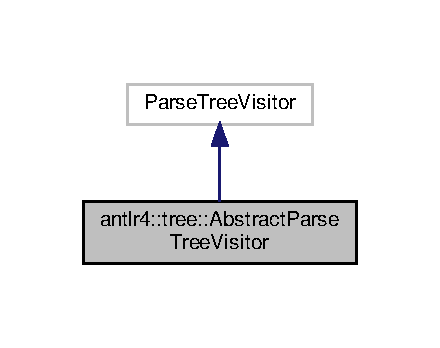
\includegraphics[width=211pt]{classantlr4_1_1tree_1_1AbstractParseTreeVisitor__inherit__graph}
\end{center}
\end{figure}


Collaboration diagram for antlr4\+:\+:tree\+:\+:Abstract\+Parse\+Tree\+Visitor\+:
\nopagebreak
\begin{figure}[H]
\begin{center}
\leavevmode
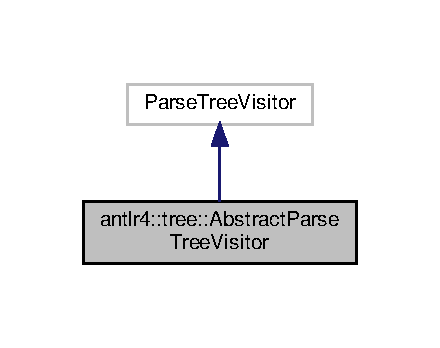
\includegraphics[width=211pt]{classantlr4_1_1tree_1_1AbstractParseTreeVisitor__coll__graph}
\end{center}
\end{figure}
\subsection*{Public Member Functions}
\begin{DoxyCompactItemize}
\item 
virtual \hyperlink{structantlrcpp_1_1Any}{antlrcpp\+::\+Any} \hyperlink{classantlr4_1_1tree_1_1AbstractParseTreeVisitor_a2f0e9c7e0c581b3ec08d59d216d7554d}{visit} (\hyperlink{classantlr4_1_1tree_1_1ParseTree}{Parse\+Tree} $\ast$tree) override
\item 
virtual \hyperlink{structantlrcpp_1_1Any}{antlrcpp\+::\+Any} \hyperlink{classantlr4_1_1tree_1_1AbstractParseTreeVisitor_a38605a51f1b8828eedb2f2ccb9e6c705}{visit\+Children} (\hyperlink{classantlr4_1_1tree_1_1ParseTree}{Parse\+Tree} $\ast$node) override
\item 
virtual \hyperlink{structantlrcpp_1_1Any}{antlrcpp\+::\+Any} \hyperlink{classantlr4_1_1tree_1_1AbstractParseTreeVisitor_a6045b85607e961bf7f364b91fd50c3ef}{visit\+Terminal} (\hyperlink{classantlr4_1_1tree_1_1TerminalNode}{Terminal\+Node} $\ast$) override
\item 
virtual \hyperlink{structantlrcpp_1_1Any}{antlrcpp\+::\+Any} \hyperlink{classantlr4_1_1tree_1_1AbstractParseTreeVisitor_a4cd5f0eaaf54140af51f1549d0a6b62d}{visit\+Error\+Node} (\hyperlink{classantlr4_1_1tree_1_1ErrorNode}{Error\+Node} $\ast$) override
\end{DoxyCompactItemize}


\subsection{Member Function Documentation}
\mbox{\Hypertarget{classantlr4_1_1tree_1_1AbstractParseTreeVisitor_a2f0e9c7e0c581b3ec08d59d216d7554d}\label{classantlr4_1_1tree_1_1AbstractParseTreeVisitor_a2f0e9c7e0c581b3ec08d59d216d7554d}} 
\index{antlr4\+::tree\+::\+Abstract\+Parse\+Tree\+Visitor@{antlr4\+::tree\+::\+Abstract\+Parse\+Tree\+Visitor}!visit@{visit}}
\index{visit@{visit}!antlr4\+::tree\+::\+Abstract\+Parse\+Tree\+Visitor@{antlr4\+::tree\+::\+Abstract\+Parse\+Tree\+Visitor}}
\subsubsection{\texorpdfstring{visit()}{visit()}}
{\footnotesize\ttfamily virtual \hyperlink{structantlrcpp_1_1Any}{antlrcpp\+::\+Any} antlr4\+::tree\+::\+Abstract\+Parse\+Tree\+Visitor\+::visit (\begin{DoxyParamCaption}\item[{\hyperlink{classantlr4_1_1tree_1_1ParseTree}{Parse\+Tree} $\ast$}]{tree }\end{DoxyParamCaption})\hspace{0.3cm}{\ttfamily [inline]}, {\ttfamily [override]}, {\ttfamily [virtual]}}

The default implementation calls \begin{DoxySeeAlso}{See also}
Parse\+Tree\+::accept


\end{DoxySeeAlso}
on the specified tree. \mbox{\Hypertarget{classantlr4_1_1tree_1_1AbstractParseTreeVisitor_a38605a51f1b8828eedb2f2ccb9e6c705}\label{classantlr4_1_1tree_1_1AbstractParseTreeVisitor_a38605a51f1b8828eedb2f2ccb9e6c705}} 
\index{antlr4\+::tree\+::\+Abstract\+Parse\+Tree\+Visitor@{antlr4\+::tree\+::\+Abstract\+Parse\+Tree\+Visitor}!visit\+Children@{visit\+Children}}
\index{visit\+Children@{visit\+Children}!antlr4\+::tree\+::\+Abstract\+Parse\+Tree\+Visitor@{antlr4\+::tree\+::\+Abstract\+Parse\+Tree\+Visitor}}
\subsubsection{\texorpdfstring{visit\+Children()}{visitChildren()}}
{\footnotesize\ttfamily virtual \hyperlink{structantlrcpp_1_1Any}{antlrcpp\+::\+Any} antlr4\+::tree\+::\+Abstract\+Parse\+Tree\+Visitor\+::visit\+Children (\begin{DoxyParamCaption}\item[{\hyperlink{classantlr4_1_1tree_1_1ParseTree}{Parse\+Tree} $\ast$}]{node }\end{DoxyParamCaption})\hspace{0.3cm}{\ttfamily [inline]}, {\ttfamily [override]}, {\ttfamily [virtual]}}

The default implementation initializes the aggregate result to \hyperlink{}{default\+Result()}. Before visiting each child, it calls \hyperlink{}{should\+Visit\+Next\+Child}; if the result is
\begin{DoxyCode}
\textcolor{keyword}{false} 
\end{DoxyCode}
 no more children are visited and the current aggregate result is returned. After visiting a child, the aggregate result is updated by calling \hyperlink{}{aggregate\+Result} with the previous aggregate result and the result of visiting the child.

The default implementation is not safe for use in visitors that modify the tree structure. Visitors that modify the tree should override this method to behave properly in respect to the specific algorithm in use.\mbox{\Hypertarget{classantlr4_1_1tree_1_1AbstractParseTreeVisitor_a4cd5f0eaaf54140af51f1549d0a6b62d}\label{classantlr4_1_1tree_1_1AbstractParseTreeVisitor_a4cd5f0eaaf54140af51f1549d0a6b62d}} 
\index{antlr4\+::tree\+::\+Abstract\+Parse\+Tree\+Visitor@{antlr4\+::tree\+::\+Abstract\+Parse\+Tree\+Visitor}!visit\+Error\+Node@{visit\+Error\+Node}}
\index{visit\+Error\+Node@{visit\+Error\+Node}!antlr4\+::tree\+::\+Abstract\+Parse\+Tree\+Visitor@{antlr4\+::tree\+::\+Abstract\+Parse\+Tree\+Visitor}}
\subsubsection{\texorpdfstring{visit\+Error\+Node()}{visitErrorNode()}}
{\footnotesize\ttfamily virtual \hyperlink{structantlrcpp_1_1Any}{antlrcpp\+::\+Any} antlr4\+::tree\+::\+Abstract\+Parse\+Tree\+Visitor\+::visit\+Error\+Node (\begin{DoxyParamCaption}\item[{\hyperlink{classantlr4_1_1tree_1_1ErrorNode}{Error\+Node} $\ast$}]{ }\end{DoxyParamCaption})\hspace{0.3cm}{\ttfamily [inline]}, {\ttfamily [override]}, {\ttfamily [virtual]}}

The default implementation returns the result of \begin{DoxySeeAlso}{See also}
\#default\+Result default\+Result


\end{DoxySeeAlso}
. \mbox{\Hypertarget{classantlr4_1_1tree_1_1AbstractParseTreeVisitor_a6045b85607e961bf7f364b91fd50c3ef}\label{classantlr4_1_1tree_1_1AbstractParseTreeVisitor_a6045b85607e961bf7f364b91fd50c3ef}} 
\index{antlr4\+::tree\+::\+Abstract\+Parse\+Tree\+Visitor@{antlr4\+::tree\+::\+Abstract\+Parse\+Tree\+Visitor}!visit\+Terminal@{visit\+Terminal}}
\index{visit\+Terminal@{visit\+Terminal}!antlr4\+::tree\+::\+Abstract\+Parse\+Tree\+Visitor@{antlr4\+::tree\+::\+Abstract\+Parse\+Tree\+Visitor}}
\subsubsection{\texorpdfstring{visit\+Terminal()}{visitTerminal()}}
{\footnotesize\ttfamily virtual \hyperlink{structantlrcpp_1_1Any}{antlrcpp\+::\+Any} antlr4\+::tree\+::\+Abstract\+Parse\+Tree\+Visitor\+::visit\+Terminal (\begin{DoxyParamCaption}\item[{\hyperlink{classantlr4_1_1tree_1_1TerminalNode}{Terminal\+Node} $\ast$}]{ }\end{DoxyParamCaption})\hspace{0.3cm}{\ttfamily [inline]}, {\ttfamily [override]}, {\ttfamily [virtual]}}

The default implementation returns the result of \begin{DoxySeeAlso}{See also}
\#default\+Result default\+Result


\end{DoxySeeAlso}
. 

The documentation for this class was generated from the following file\+:\begin{DoxyCompactItemize}
\item 
tree/Abstract\+Parse\+Tree\+Visitor.\+h\end{DoxyCompactItemize}

\hypertarget{classantlr4_1_1atn_1_1AbstractPredicateTransition}{}\section{antlr4\+:\+:atn\+:\+:Abstract\+Predicate\+Transition Class Reference}
\label{classantlr4_1_1atn_1_1AbstractPredicateTransition}\index{antlr4\+::atn\+::\+Abstract\+Predicate\+Transition@{antlr4\+::atn\+::\+Abstract\+Predicate\+Transition}}


Inheritance diagram for antlr4\+:\+:atn\+:\+:Abstract\+Predicate\+Transition\+:
\nopagebreak
\begin{figure}[H]
\begin{center}
\leavevmode
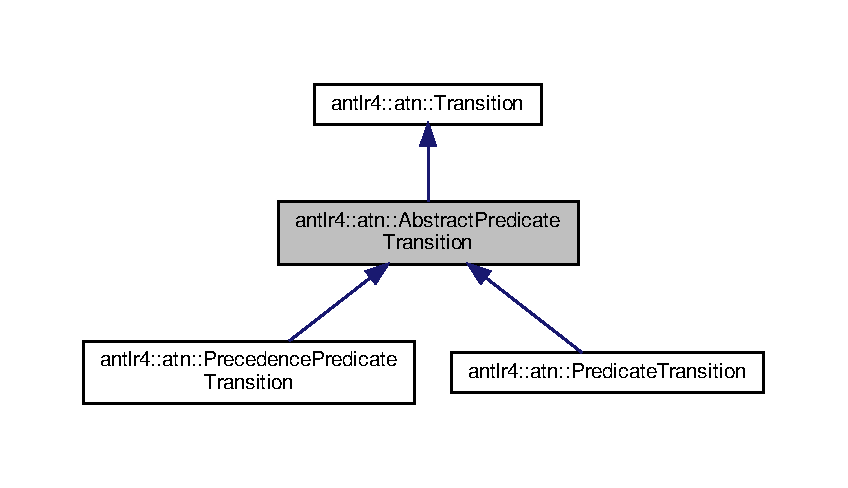
\includegraphics[width=350pt]{classantlr4_1_1atn_1_1AbstractPredicateTransition__inherit__graph}
\end{center}
\end{figure}


Collaboration diagram for antlr4\+:\+:atn\+:\+:Abstract\+Predicate\+Transition\+:
\nopagebreak
\begin{figure}[H]
\begin{center}
\leavevmode
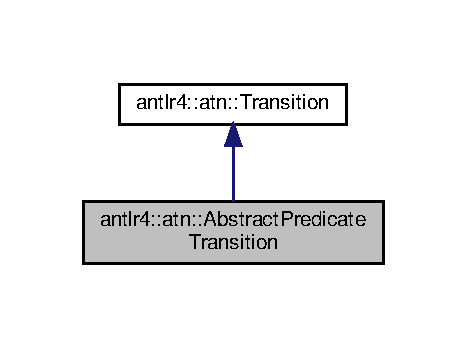
\includegraphics[width=224pt]{classantlr4_1_1atn_1_1AbstractPredicateTransition__coll__graph}
\end{center}
\end{figure}
\subsection*{Public Member Functions}
\begin{DoxyCompactItemize}
\item 
\mbox{\Hypertarget{classantlr4_1_1atn_1_1AbstractPredicateTransition_a063926aaf5651de84080aaa801e67e50}\label{classantlr4_1_1atn_1_1AbstractPredicateTransition_a063926aaf5651de84080aaa801e67e50}} 
{\bfseries Abstract\+Predicate\+Transition} (A\+T\+N\+State $\ast$\hyperlink{classantlr4_1_1atn_1_1Transition_aaaed7f4ddda71e156b36de33e88f66a7}{target})
\end{DoxyCompactItemize}
\subsection*{Additional Inherited Members}


The documentation for this class was generated from the following files\+:\begin{DoxyCompactItemize}
\item 
atn/Abstract\+Predicate\+Transition.\+h\item 
atn/Abstract\+Predicate\+Transition.\+cpp\end{DoxyCompactItemize}

\hypertarget{classantlr4_1_1atn_1_1ActionTransition}{}\section{antlr4\+:\+:atn\+:\+:Action\+Transition Class Reference}
\label{classantlr4_1_1atn_1_1ActionTransition}\index{antlr4\+::atn\+::\+Action\+Transition@{antlr4\+::atn\+::\+Action\+Transition}}


Inheritance diagram for antlr4\+:\+:atn\+:\+:Action\+Transition\+:
\nopagebreak
\begin{figure}[H]
\begin{center}
\leavevmode
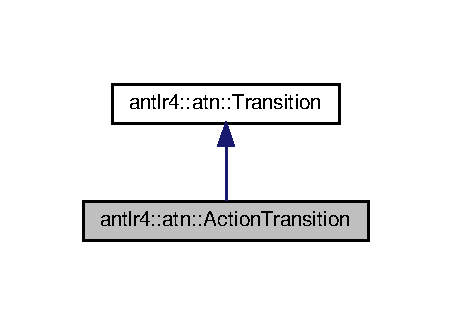
\includegraphics[width=217pt]{classantlr4_1_1atn_1_1ActionTransition__inherit__graph}
\end{center}
\end{figure}


Collaboration diagram for antlr4\+:\+:atn\+:\+:Action\+Transition\+:
\nopagebreak
\begin{figure}[H]
\begin{center}
\leavevmode
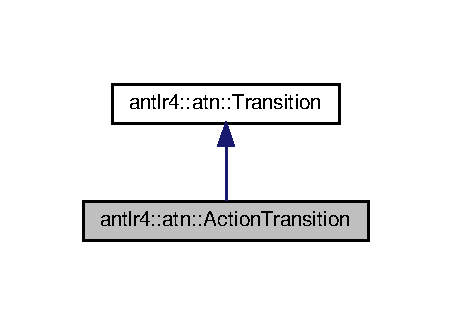
\includegraphics[width=217pt]{classantlr4_1_1atn_1_1ActionTransition__coll__graph}
\end{center}
\end{figure}
\subsection*{Public Member Functions}
\begin{DoxyCompactItemize}
\item 
\mbox{\Hypertarget{classantlr4_1_1atn_1_1ActionTransition_a2771f493d91a6537b4edd0be5ead778f}\label{classantlr4_1_1atn_1_1ActionTransition_a2771f493d91a6537b4edd0be5ead778f}} 
{\bfseries Action\+Transition} (A\+T\+N\+State $\ast$\hyperlink{classantlr4_1_1atn_1_1Transition_aaaed7f4ddda71e156b36de33e88f66a7}{target}, size\+\_\+t rule\+Index)
\item 
\mbox{\Hypertarget{classantlr4_1_1atn_1_1ActionTransition_a9db50574aa1160b0286d5677f2bf76a4}\label{classantlr4_1_1atn_1_1ActionTransition_a9db50574aa1160b0286d5677f2bf76a4}} 
{\bfseries Action\+Transition} (A\+T\+N\+State $\ast$\hyperlink{classantlr4_1_1atn_1_1Transition_aaaed7f4ddda71e156b36de33e88f66a7}{target}, size\+\_\+t rule\+Index, size\+\_\+t action\+Index, bool is\+Ctx\+Dependent)
\item 
\mbox{\Hypertarget{classantlr4_1_1atn_1_1ActionTransition_a25ce773af6ba3e4c0a582bf92f1f762d}\label{classantlr4_1_1atn_1_1ActionTransition_a25ce773af6ba3e4c0a582bf92f1f762d}} 
virtual Serialization\+Type {\bfseries get\+Serialization\+Type} () const override
\item 
virtual bool \hyperlink{classantlr4_1_1atn_1_1ActionTransition_a995b2814e1d1751f39655f6856572584}{is\+Epsilon} () const override
\item 
\mbox{\Hypertarget{classantlr4_1_1atn_1_1ActionTransition_a4f37aaaacdfa869ed9fc2bfd18c4c4f1}\label{classantlr4_1_1atn_1_1ActionTransition_a4f37aaaacdfa869ed9fc2bfd18c4c4f1}} 
virtual bool {\bfseries matches} (size\+\_\+t symbol, size\+\_\+t min\+Vocab\+Symbol, size\+\_\+t max\+Vocab\+Symbol) const override
\item 
\mbox{\Hypertarget{classantlr4_1_1atn_1_1ActionTransition_ac6073b34445e5c7e8725801bb2f08fac}\label{classantlr4_1_1atn_1_1ActionTransition_ac6073b34445e5c7e8725801bb2f08fac}} 
virtual std\+::string {\bfseries to\+String} () const override
\end{DoxyCompactItemize}
\subsection*{Public Attributes}
\begin{DoxyCompactItemize}
\item 
\mbox{\Hypertarget{classantlr4_1_1atn_1_1ActionTransition_a7da8a981b5daec5c8071a653c5a36fc9}\label{classantlr4_1_1atn_1_1ActionTransition_a7da8a981b5daec5c8071a653c5a36fc9}} 
const size\+\_\+t {\bfseries rule\+Index}
\item 
\mbox{\Hypertarget{classantlr4_1_1atn_1_1ActionTransition_a905ea817ee87fee14169bfa474342b60}\label{classantlr4_1_1atn_1_1ActionTransition_a905ea817ee87fee14169bfa474342b60}} 
const size\+\_\+t {\bfseries action\+Index}
\item 
\mbox{\Hypertarget{classantlr4_1_1atn_1_1ActionTransition_aba0631ffdeba1c944dfd22cd3a5b68b4}\label{classantlr4_1_1atn_1_1ActionTransition_aba0631ffdeba1c944dfd22cd3a5b68b4}} 
const bool {\bfseries is\+Ctx\+Dependent}
\end{DoxyCompactItemize}
\subsection*{Additional Inherited Members}


\subsection{Member Function Documentation}
\mbox{\Hypertarget{classantlr4_1_1atn_1_1ActionTransition_a995b2814e1d1751f39655f6856572584}\label{classantlr4_1_1atn_1_1ActionTransition_a995b2814e1d1751f39655f6856572584}} 
\index{antlr4\+::atn\+::\+Action\+Transition@{antlr4\+::atn\+::\+Action\+Transition}!is\+Epsilon@{is\+Epsilon}}
\index{is\+Epsilon@{is\+Epsilon}!antlr4\+::atn\+::\+Action\+Transition@{antlr4\+::atn\+::\+Action\+Transition}}
\subsubsection{\texorpdfstring{is\+Epsilon()}{isEpsilon()}}
{\footnotesize\ttfamily bool Action\+Transition\+::is\+Epsilon (\begin{DoxyParamCaption}{ }\end{DoxyParamCaption}) const\hspace{0.3cm}{\ttfamily [override]}, {\ttfamily [virtual]}}

Determines if the transition is an \char`\"{}epsilon\char`\"{} transition.

The default implementation returns
\begin{DoxyCode}
\textcolor{keyword}{false} 
\end{DoxyCode}
 .

\begin{DoxyReturn}{Returns}

\begin{DoxyCode}
\textcolor{keyword}{true} 
\end{DoxyCode}
 if traversing this transition in the A\+TN does not consume an input symbol; otherwise,
\begin{DoxyCode}
\textcolor{keyword}{false} 
\end{DoxyCode}
 if traversing this transition consumes (matches) an input symbol. 
\end{DoxyReturn}


Reimplemented from \hyperlink{classantlr4_1_1atn_1_1Transition_a8e712c7a46586d73c054c56f481b1be7}{antlr4\+::atn\+::\+Transition}.



The documentation for this class was generated from the following files\+:\begin{DoxyCompactItemize}
\item 
atn/Action\+Transition.\+h\item 
atn/Action\+Transition.\+cpp\end{DoxyCompactItemize}

\hypertarget{structAltAndContextConfigComparer}{}\section{Alt\+And\+Context\+Config\+Comparer Struct Reference}
\label{structAltAndContextConfigComparer}\index{Alt\+And\+Context\+Config\+Comparer@{Alt\+And\+Context\+Config\+Comparer}}
\subsection*{Public Member Functions}
\begin{DoxyCompactItemize}
\item 
\mbox{\Hypertarget{structAltAndContextConfigComparer_aa6634e7afe86651ba29db08b186513d4}\label{structAltAndContextConfigComparer_aa6634e7afe86651ba29db08b186513d4}} 
bool {\bfseries operator()} (\hyperlink{classantlr4_1_1atn_1_1ATNConfig}{A\+T\+N\+Config} $\ast$a, \hyperlink{classantlr4_1_1atn_1_1ATNConfig}{A\+T\+N\+Config} $\ast$b) const
\end{DoxyCompactItemize}


The documentation for this struct was generated from the following file\+:\begin{DoxyCompactItemize}
\item 
atn/Prediction\+Mode.\+cpp\end{DoxyCompactItemize}

\hypertarget{structAltAndContextConfigHasher}{}\section{Alt\+And\+Context\+Config\+Hasher Struct Reference}
\label{structAltAndContextConfigHasher}\index{Alt\+And\+Context\+Config\+Hasher@{Alt\+And\+Context\+Config\+Hasher}}
\subsection*{Public Member Functions}
\begin{DoxyCompactItemize}
\item 
size\+\_\+t \hyperlink{structAltAndContextConfigHasher_aaff11232d12d08e88422318bff2ba22f}{operator()} (\hyperlink{classantlr4_1_1atn_1_1ATNConfig}{A\+T\+N\+Config} $\ast$o) const
\end{DoxyCompactItemize}


\subsection{Member Function Documentation}
\mbox{\Hypertarget{structAltAndContextConfigHasher_aaff11232d12d08e88422318bff2ba22f}\label{structAltAndContextConfigHasher_aaff11232d12d08e88422318bff2ba22f}} 
\index{Alt\+And\+Context\+Config\+Hasher@{Alt\+And\+Context\+Config\+Hasher}!operator()@{operator()}}
\index{operator()@{operator()}!Alt\+And\+Context\+Config\+Hasher@{Alt\+And\+Context\+Config\+Hasher}}
\subsubsection{\texorpdfstring{operator()()}{operator()()}}
{\footnotesize\ttfamily size\+\_\+t Alt\+And\+Context\+Config\+Hasher\+::operator() (\begin{DoxyParamCaption}\item[{\hyperlink{classantlr4_1_1atn_1_1ATNConfig}{A\+T\+N\+Config} $\ast$}]{o }\end{DoxyParamCaption}) const\hspace{0.3cm}{\ttfamily [inline]}}

The hash code is only a function of the \hyperlink{}{A\+T\+N\+State\#state\+Number} and \hyperlink{}{A\+T\+N\+Config\#context}. 

The documentation for this struct was generated from the following file\+:\begin{DoxyCompactItemize}
\item 
atn/Prediction\+Mode.\+cpp\end{DoxyCompactItemize}

\hypertarget{classantlr4_1_1ANTLRErrorListener}{}\section{antlr4\+:\+:A\+N\+T\+L\+R\+Error\+Listener Class Reference}
\label{classantlr4_1_1ANTLRErrorListener}\index{antlr4\+::\+A\+N\+T\+L\+R\+Error\+Listener@{antlr4\+::\+A\+N\+T\+L\+R\+Error\+Listener}}


How to emit recognition errors (an interface in Java).  




{\ttfamily \#include $<$A\+N\+T\+L\+R\+Error\+Listener.\+h$>$}



Inheritance diagram for antlr4\+:\+:A\+N\+T\+L\+R\+Error\+Listener\+:
\nopagebreak
\begin{figure}[H]
\begin{center}
\leavevmode
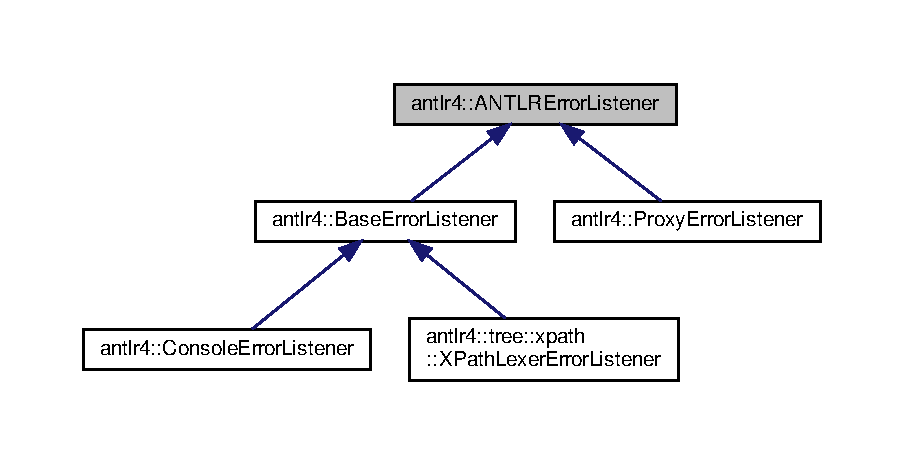
\includegraphics[width=350pt]{classantlr4_1_1ANTLRErrorListener__inherit__graph}
\end{center}
\end{figure}


\subsection{Detailed Description}
How to emit recognition errors (an interface in Java). 

The documentation for this class was generated from the following files\+:\begin{DoxyCompactItemize}
\item 
A\+N\+T\+L\+R\+Error\+Listener.\+h\item 
A\+N\+T\+L\+R\+Error\+Listener.\+cpp\end{DoxyCompactItemize}

\hypertarget{classantlr4_1_1ANTLRErrorStrategy}{}\section{antlr4\+:\+:A\+N\+T\+L\+R\+Error\+Strategy Class Reference}
\label{classantlr4_1_1ANTLRErrorStrategy}\index{antlr4\+::\+A\+N\+T\+L\+R\+Error\+Strategy@{antlr4\+::\+A\+N\+T\+L\+R\+Error\+Strategy}}


The interface for defining strategies to deal with syntax errors encountered during a parse by A\+N\+T\+L\+R-\/generated parsers. We distinguish between three different kinds of errors\+:  




{\ttfamily \#include $<$A\+N\+T\+L\+R\+Error\+Strategy.\+h$>$}



Inheritance diagram for antlr4\+:\+:A\+N\+T\+L\+R\+Error\+Strategy\+:
\nopagebreak
\begin{figure}[H]
\begin{center}
\leavevmode
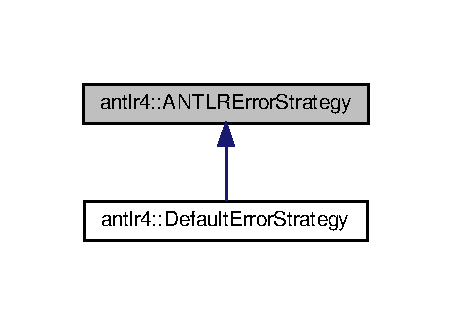
\includegraphics[width=217pt]{classantlr4_1_1ANTLRErrorStrategy__inherit__graph}
\end{center}
\end{figure}


\subsection{Detailed Description}
The interface for defining strategies to deal with syntax errors encountered during a parse by A\+N\+T\+L\+R-\/generated parsers. We distinguish between three different kinds of errors\+: 


\begin{DoxyItemize}
\item The parser could not figure out which path to take in the A\+TN (none of the available alternatives could possibly match) 
\item The current input does not match what we were looking for 
\item A predicate evaluated to false 
\end{DoxyItemize}

Implementations of this interface report syntax errors by calling \begin{DoxySeeAlso}{See also}
Parser\+::notify\+Error\+Listeners


\end{DoxySeeAlso}
. 

T\+O\+\_\+\+DO\+: what to do about lexers 

The documentation for this class was generated from the following file\+:\begin{DoxyCompactItemize}
\item 
A\+N\+T\+L\+R\+Error\+Strategy.\+h\end{DoxyCompactItemize}

\hypertarget{classantlr4_1_1ANTLRFileStream}{}\section{antlr4\+:\+:A\+N\+T\+L\+R\+File\+Stream Class Reference}
\label{classantlr4_1_1ANTLRFileStream}\index{antlr4\+::\+A\+N\+T\+L\+R\+File\+Stream@{antlr4\+::\+A\+N\+T\+L\+R\+File\+Stream}}


{\ttfamily \#include $<$A\+N\+T\+L\+R\+File\+Stream.\+h$>$}



Inheritance diagram for antlr4\+:\+:A\+N\+T\+L\+R\+File\+Stream\+:
\nopagebreak
\begin{figure}[H]
\begin{center}
\leavevmode
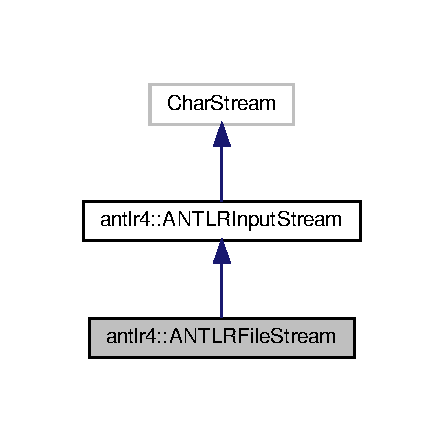
\includegraphics[width=213pt]{classantlr4_1_1ANTLRFileStream__inherit__graph}
\end{center}
\end{figure}


Collaboration diagram for antlr4\+:\+:A\+N\+T\+L\+R\+File\+Stream\+:
\nopagebreak
\begin{figure}[H]
\begin{center}
\leavevmode
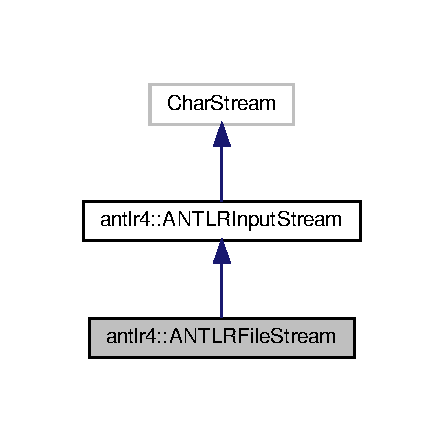
\includegraphics[width=213pt]{classantlr4_1_1ANTLRFileStream__coll__graph}
\end{center}
\end{figure}
\subsection*{Public Member Functions}
\begin{DoxyCompactItemize}
\item 
\mbox{\Hypertarget{classantlr4_1_1ANTLRFileStream_ae73684208e79d7cb7d563bc3682a6245}\label{classantlr4_1_1ANTLRFileStream_ae73684208e79d7cb7d563bc3682a6245}} 
{\bfseries A\+N\+T\+L\+R\+File\+Stream} (const std\+::string \&file\+Name)
\item 
\mbox{\Hypertarget{classantlr4_1_1ANTLRFileStream_ae8d8fcf45ba9498dcba5d4664fea76ad}\label{classantlr4_1_1ANTLRFileStream_ae8d8fcf45ba9498dcba5d4664fea76ad}} 
virtual void {\bfseries load\+From\+File} (const std\+::string \&file\+Name)
\item 
\mbox{\Hypertarget{classantlr4_1_1ANTLRFileStream_a9c3954984c435d8e1a2a9bb898017486}\label{classantlr4_1_1ANTLRFileStream_a9c3954984c435d8e1a2a9bb898017486}} 
virtual std\+::string {\bfseries get\+Source\+Name} () const override
\end{DoxyCompactItemize}
\subsection*{Protected Attributes}
\begin{DoxyCompactItemize}
\item 
\mbox{\Hypertarget{classantlr4_1_1ANTLRFileStream_a0b0c3fc70ad26d5bda57cbdfc503198e}\label{classantlr4_1_1ANTLRFileStream_a0b0c3fc70ad26d5bda57cbdfc503198e}} 
std\+::string {\bfseries \+\_\+file\+Name}
\end{DoxyCompactItemize}
\subsection*{Additional Inherited Members}


\subsection{Detailed Description}
This is an \hyperlink{classantlr4_1_1ANTLRInputStream}{A\+N\+T\+L\+R\+Input\+Stream} that is loaded from a file all at once when you construct the object (or call load()). 

The documentation for this class was generated from the following files\+:\begin{DoxyCompactItemize}
\item 
A\+N\+T\+L\+R\+File\+Stream.\+h\item 
A\+N\+T\+L\+R\+File\+Stream.\+cpp\end{DoxyCompactItemize}

\hypertarget{classantlr4_1_1ANTLRInputStream}{}\section{antlr4\+:\+:A\+N\+T\+L\+R\+Input\+Stream Class Reference}
\label{classantlr4_1_1ANTLRInputStream}\index{antlr4\+::\+A\+N\+T\+L\+R\+Input\+Stream@{antlr4\+::\+A\+N\+T\+L\+R\+Input\+Stream}}


Inheritance diagram for antlr4\+:\+:A\+N\+T\+L\+R\+Input\+Stream\+:
\nopagebreak
\begin{figure}[H]
\begin{center}
\leavevmode
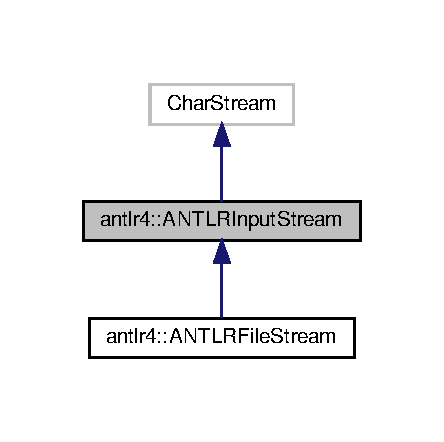
\includegraphics[width=213pt]{classantlr4_1_1ANTLRInputStream__inherit__graph}
\end{center}
\end{figure}


Collaboration diagram for antlr4\+:\+:A\+N\+T\+L\+R\+Input\+Stream\+:
\nopagebreak
\begin{figure}[H]
\begin{center}
\leavevmode
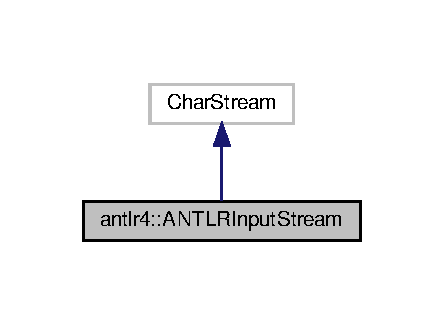
\includegraphics[width=213pt]{classantlr4_1_1ANTLRInputStream__coll__graph}
\end{center}
\end{figure}
\subsection*{Public Member Functions}
\begin{DoxyCompactItemize}
\item 
\mbox{\Hypertarget{classantlr4_1_1ANTLRInputStream_a94e7ae64a3b2d80f911fdb81807efd74}\label{classantlr4_1_1ANTLRInputStream_a94e7ae64a3b2d80f911fdb81807efd74}} 
{\bfseries A\+N\+T\+L\+R\+Input\+Stream} (const std\+::string \&input=\char`\"{}\char`\"{})
\item 
\mbox{\Hypertarget{classantlr4_1_1ANTLRInputStream_aba79908d868c1cd00081885d8ff968e7}\label{classantlr4_1_1ANTLRInputStream_aba79908d868c1cd00081885d8ff968e7}} 
{\bfseries A\+N\+T\+L\+R\+Input\+Stream} (const char data\+\_\+\mbox{[}$\,$\mbox{]}, size\+\_\+t number\+Of\+Actual\+Chars\+In\+Array)
\item 
\mbox{\Hypertarget{classantlr4_1_1ANTLRInputStream_aef56607c326c48eebce3bf7202608240}\label{classantlr4_1_1ANTLRInputStream_aef56607c326c48eebce3bf7202608240}} 
{\bfseries A\+N\+T\+L\+R\+Input\+Stream} (std\+::istream \&stream)
\item 
\mbox{\Hypertarget{classantlr4_1_1ANTLRInputStream_ae962ece9c34a19c1aeb5100ccab8b81a}\label{classantlr4_1_1ANTLRInputStream_ae962ece9c34a19c1aeb5100ccab8b81a}} 
virtual void {\bfseries load} (const std\+::string \&input)
\item 
\mbox{\Hypertarget{classantlr4_1_1ANTLRInputStream_a5806e604d09aaffa6a0d818024c30484}\label{classantlr4_1_1ANTLRInputStream_a5806e604d09aaffa6a0d818024c30484}} 
virtual void {\bfseries load} (std\+::istream \&stream)
\item 
virtual void \hyperlink{classantlr4_1_1ANTLRInputStream_a3bb10995cd48f3fe06f6399a43d4bbb9}{reset} ()
\item 
\mbox{\Hypertarget{classantlr4_1_1ANTLRInputStream_a8edddb1d103e27801c98211acf482f67}\label{classantlr4_1_1ANTLRInputStream_a8edddb1d103e27801c98211acf482f67}} 
virtual void {\bfseries consume} () override
\item 
\mbox{\Hypertarget{classantlr4_1_1ANTLRInputStream_afa8fc0a6689cc0ce807dfc06c89bae9d}\label{classantlr4_1_1ANTLRInputStream_afa8fc0a6689cc0ce807dfc06c89bae9d}} 
virtual size\+\_\+t {\bfseries LA} (ssize\+\_\+t i) override
\item 
\mbox{\Hypertarget{classantlr4_1_1ANTLRInputStream_ad7f3adaa1b600c90f0f59531ef4b75a1}\label{classantlr4_1_1ANTLRInputStream_ad7f3adaa1b600c90f0f59531ef4b75a1}} 
virtual size\+\_\+t {\bfseries LT} (ssize\+\_\+t i)
\item 
virtual size\+\_\+t \hyperlink{classantlr4_1_1ANTLRInputStream_a4c9a7beab5662a33a537fa49fc27db9f}{index} () override
\begin{DoxyCompactList}\small\item\em Return the current input symbol index 0..n where n indicates the last symbol has been read. The index is the index of char to be returned from L\+A(1). \end{DoxyCompactList}\item 
\mbox{\Hypertarget{classantlr4_1_1ANTLRInputStream_ae96b37a6b345a0f637058890d4c97cf6}\label{classantlr4_1_1ANTLRInputStream_ae96b37a6b345a0f637058890d4c97cf6}} 
virtual size\+\_\+t {\bfseries size} () override
\item 
virtual ssize\+\_\+t \hyperlink{classantlr4_1_1ANTLRInputStream_a5a1520d6417bef7e06cb8d524ec6f76c}{mark} () override
\begin{DoxyCompactList}\small\item\em mark/release do nothing; we have entire buffer \end{DoxyCompactList}\item 
\mbox{\Hypertarget{classantlr4_1_1ANTLRInputStream_ab376abfc892d24098cc45fc3917acac0}\label{classantlr4_1_1ANTLRInputStream_ab376abfc892d24098cc45fc3917acac0}} 
virtual void {\bfseries release} (ssize\+\_\+t marker) override
\item 
virtual void \hyperlink{classantlr4_1_1ANTLRInputStream_ac46f2e88f0772bc65b537781a2341010}{seek} (size\+\_\+t \hyperlink{classantlr4_1_1ANTLRInputStream_a4c9a7beab5662a33a537fa49fc27db9f}{index}) override
\begin{DoxyCompactList}\small\item\em consume() ahead until p==index; can\textquotesingle{}t just set p=index as we must update line and char\+Position\+In\+Line. If we seek backwards, just set p \end{DoxyCompactList}\item 
\mbox{\Hypertarget{classantlr4_1_1ANTLRInputStream_a24450f62298de76d6a8bc251540d79c2}\label{classantlr4_1_1ANTLRInputStream_a24450f62298de76d6a8bc251540d79c2}} 
virtual std\+::string {\bfseries get\+Text} (const \hyperlink{classantlr4_1_1misc_1_1Interval}{misc\+::\+Interval} \&interval) override
\item 
\mbox{\Hypertarget{classantlr4_1_1ANTLRInputStream_a4f2208f3974b6c153bf561d0addb88f3}\label{classantlr4_1_1ANTLRInputStream_a4f2208f3974b6c153bf561d0addb88f3}} 
virtual std\+::string {\bfseries get\+Source\+Name} () const override
\item 
\mbox{\Hypertarget{classantlr4_1_1ANTLRInputStream_a93b3e3b667734ad0c4cf4c5058e9b7cb}\label{classantlr4_1_1ANTLRInputStream_a93b3e3b667734ad0c4cf4c5058e9b7cb}} 
virtual std\+::string {\bfseries to\+String} () const override
\end{DoxyCompactItemize}
\subsection*{Public Attributes}
\begin{DoxyCompactItemize}
\item 
\mbox{\Hypertarget{classantlr4_1_1ANTLRInputStream_a484ecb90c871af2b7ccd364720caf4ee}\label{classantlr4_1_1ANTLRInputStream_a484ecb90c871af2b7ccd364720caf4ee}} 
std\+::string \hyperlink{classantlr4_1_1ANTLRInputStream_a484ecb90c871af2b7ccd364720caf4ee}{name}
\begin{DoxyCompactList}\small\item\em What is name or source of this char stream? \end{DoxyCompactList}\end{DoxyCompactItemize}
\subsection*{Protected Attributes}
\begin{DoxyCompactItemize}
\item 
\mbox{\Hypertarget{classantlr4_1_1ANTLRInputStream_ad5187c1a38d8118cb4814db0b8178a6b}\label{classantlr4_1_1ANTLRInputStream_ad5187c1a38d8118cb4814db0b8178a6b}} 
U\+T\+F32\+String \hyperlink{classantlr4_1_1ANTLRInputStream_ad5187c1a38d8118cb4814db0b8178a6b}{\+\_\+data}
\begin{DoxyCompactList}\small\item\em The data being scanned. \end{DoxyCompactList}\item 
size\+\_\+t \hyperlink{classantlr4_1_1ANTLRInputStream_a9499bf048c340771ad5f899a721c7f8d}{p}
\begin{DoxyCompactList}\small\item\em 0..n-\/1 index into string of next char \end{DoxyCompactList}\end{DoxyCompactItemize}


\subsection{Member Function Documentation}
\mbox{\Hypertarget{classantlr4_1_1ANTLRInputStream_a4c9a7beab5662a33a537fa49fc27db9f}\label{classantlr4_1_1ANTLRInputStream_a4c9a7beab5662a33a537fa49fc27db9f}} 
\index{antlr4\+::\+A\+N\+T\+L\+R\+Input\+Stream@{antlr4\+::\+A\+N\+T\+L\+R\+Input\+Stream}!index@{index}}
\index{index@{index}!antlr4\+::\+A\+N\+T\+L\+R\+Input\+Stream@{antlr4\+::\+A\+N\+T\+L\+R\+Input\+Stream}}
\subsubsection{\texorpdfstring{index()}{index()}}
{\footnotesize\ttfamily size\+\_\+t A\+N\+T\+L\+R\+Input\+Stream\+::index (\begin{DoxyParamCaption}{ }\end{DoxyParamCaption})\hspace{0.3cm}{\ttfamily [override]}, {\ttfamily [virtual]}}



Return the current input symbol index 0..n where n indicates the last symbol has been read. The index is the index of char to be returned from L\+A(1). 

\mbox{\Hypertarget{classantlr4_1_1ANTLRInputStream_a5a1520d6417bef7e06cb8d524ec6f76c}\label{classantlr4_1_1ANTLRInputStream_a5a1520d6417bef7e06cb8d524ec6f76c}} 
\index{antlr4\+::\+A\+N\+T\+L\+R\+Input\+Stream@{antlr4\+::\+A\+N\+T\+L\+R\+Input\+Stream}!mark@{mark}}
\index{mark@{mark}!antlr4\+::\+A\+N\+T\+L\+R\+Input\+Stream@{antlr4\+::\+A\+N\+T\+L\+R\+Input\+Stream}}
\subsubsection{\texorpdfstring{mark()}{mark()}}
{\footnotesize\ttfamily ssize\+\_\+t A\+N\+T\+L\+R\+Input\+Stream\+::mark (\begin{DoxyParamCaption}{ }\end{DoxyParamCaption})\hspace{0.3cm}{\ttfamily [override]}, {\ttfamily [virtual]}}



mark/release do nothing; we have entire buffer 

\mbox{\Hypertarget{classantlr4_1_1ANTLRInputStream_a3bb10995cd48f3fe06f6399a43d4bbb9}\label{classantlr4_1_1ANTLRInputStream_a3bb10995cd48f3fe06f6399a43d4bbb9}} 
\index{antlr4\+::\+A\+N\+T\+L\+R\+Input\+Stream@{antlr4\+::\+A\+N\+T\+L\+R\+Input\+Stream}!reset@{reset}}
\index{reset@{reset}!antlr4\+::\+A\+N\+T\+L\+R\+Input\+Stream@{antlr4\+::\+A\+N\+T\+L\+R\+Input\+Stream}}
\subsubsection{\texorpdfstring{reset()}{reset()}}
{\footnotesize\ttfamily void A\+N\+T\+L\+R\+Input\+Stream\+::reset (\begin{DoxyParamCaption}{ }\end{DoxyParamCaption})\hspace{0.3cm}{\ttfamily [virtual]}}

Reset the stream so that it\textquotesingle{}s in the same state it was when the object was created {\itshape except} the data array is not touched. \mbox{\Hypertarget{classantlr4_1_1ANTLRInputStream_ac46f2e88f0772bc65b537781a2341010}\label{classantlr4_1_1ANTLRInputStream_ac46f2e88f0772bc65b537781a2341010}} 
\index{antlr4\+::\+A\+N\+T\+L\+R\+Input\+Stream@{antlr4\+::\+A\+N\+T\+L\+R\+Input\+Stream}!seek@{seek}}
\index{seek@{seek}!antlr4\+::\+A\+N\+T\+L\+R\+Input\+Stream@{antlr4\+::\+A\+N\+T\+L\+R\+Input\+Stream}}
\subsubsection{\texorpdfstring{seek()}{seek()}}
{\footnotesize\ttfamily void A\+N\+T\+L\+R\+Input\+Stream\+::seek (\begin{DoxyParamCaption}\item[{size\+\_\+t}]{index }\end{DoxyParamCaption})\hspace{0.3cm}{\ttfamily [override]}, {\ttfamily [virtual]}}



consume() ahead until p==index; can\textquotesingle{}t just set p=index as we must update line and char\+Position\+In\+Line. If we seek backwards, just set p 



\subsection{Member Data Documentation}
\mbox{\Hypertarget{classantlr4_1_1ANTLRInputStream_a9499bf048c340771ad5f899a721c7f8d}\label{classantlr4_1_1ANTLRInputStream_a9499bf048c340771ad5f899a721c7f8d}} 
\index{antlr4\+::\+A\+N\+T\+L\+R\+Input\+Stream@{antlr4\+::\+A\+N\+T\+L\+R\+Input\+Stream}!p@{p}}
\index{p@{p}!antlr4\+::\+A\+N\+T\+L\+R\+Input\+Stream@{antlr4\+::\+A\+N\+T\+L\+R\+Input\+Stream}}
\subsubsection{\texorpdfstring{p}{p}}
{\footnotesize\ttfamily size\+\_\+t antlr4\+::\+A\+N\+T\+L\+R\+Input\+Stream\+::p\hspace{0.3cm}{\ttfamily [protected]}}



0..n-\/1 index into string of next char 



The documentation for this class was generated from the following files\+:\begin{DoxyCompactItemize}
\item 
A\+N\+T\+L\+R\+Input\+Stream.\+h\item 
A\+N\+T\+L\+R\+Input\+Stream.\+cpp\end{DoxyCompactItemize}

\hypertarget{structantlrcpp_1_1Any}{}\section{antlrcpp\+:\+:Any Struct Reference}
\label{structantlrcpp_1_1Any}\index{antlrcpp\+::\+Any@{antlrcpp\+::\+Any}}
\subsection*{Public Member Functions}
\begin{DoxyCompactItemize}
\item 
\mbox{\Hypertarget{structantlrcpp_1_1Any_a488abcfa917d0b5f21d1cf2285d81d78}\label{structantlrcpp_1_1Any_a488abcfa917d0b5f21d1cf2285d81d78}} 
bool {\bfseries is\+Null} () const
\item 
\mbox{\Hypertarget{structantlrcpp_1_1Any_aab5861927c245ac28e12a52070b9ef53}\label{structantlrcpp_1_1Any_aab5861927c245ac28e12a52070b9ef53}} 
bool {\bfseries is\+Not\+Null} () const
\item 
\mbox{\Hypertarget{structantlrcpp_1_1Any_a6db4c547cf9d695026921fce77bd92a8}\label{structantlrcpp_1_1Any_a6db4c547cf9d695026921fce77bd92a8}} 
{\bfseries Any} (\hyperlink{structantlrcpp_1_1Any}{Any} \&that)
\item 
\mbox{\Hypertarget{structantlrcpp_1_1Any_ade1fdb5cbfb0644de4eda2d841919718}\label{structantlrcpp_1_1Any_ade1fdb5cbfb0644de4eda2d841919718}} 
{\bfseries Any} (\hyperlink{structantlrcpp_1_1Any}{Any} \&\&that)
\item 
\mbox{\Hypertarget{structantlrcpp_1_1Any_ac68708017cd38b6552f2fd717e9fc516}\label{structantlrcpp_1_1Any_ac68708017cd38b6552f2fd717e9fc516}} 
{\bfseries Any} (const \hyperlink{structantlrcpp_1_1Any}{Any} \&that)
\item 
\mbox{\Hypertarget{structantlrcpp_1_1Any_a17ea655ba8aeaeef80c0d6b838be2e47}\label{structantlrcpp_1_1Any_a17ea655ba8aeaeef80c0d6b838be2e47}} 
{\bfseries Any} (const \hyperlink{structantlrcpp_1_1Any}{Any} \&\&that)
\item 
\mbox{\Hypertarget{structantlrcpp_1_1Any_a6124bb282c372a197d0d1182e1278ef9}\label{structantlrcpp_1_1Any_a6124bb282c372a197d0d1182e1278ef9}} 
{\footnotesize template$<$typename U $>$ }\\{\bfseries Any} (U \&\&value)
\item 
\mbox{\Hypertarget{structantlrcpp_1_1Any_a24ead6d715354e80c5fddc3337cac100}\label{structantlrcpp_1_1Any_a24ead6d715354e80c5fddc3337cac100}} 
{\footnotesize template$<$class U $>$ }\\bool {\bfseries is} () const
\item 
\mbox{\Hypertarget{structantlrcpp_1_1Any_a1601333b7a6f2946c6a9574b4c048bb9}\label{structantlrcpp_1_1Any_a1601333b7a6f2946c6a9574b4c048bb9}} 
{\footnotesize template$<$class U $>$ }\\Storage\+Type$<$ U $>$ \& {\bfseries as} ()
\item 
\mbox{\Hypertarget{structantlrcpp_1_1Any_a0ea0d91dadd5bd8040658cdc884bf9bd}\label{structantlrcpp_1_1Any_a0ea0d91dadd5bd8040658cdc884bf9bd}} 
{\footnotesize template$<$class U $>$ }\\const Storage\+Type$<$ U $>$ \& {\bfseries as} () const
\item 
\mbox{\Hypertarget{structantlrcpp_1_1Any_aab7d8365f55c4e7cf4def8cd8269bd14}\label{structantlrcpp_1_1Any_aab7d8365f55c4e7cf4def8cd8269bd14}} 
{\footnotesize template$<$class U $>$ }\\{\bfseries operator U} ()
\item 
\mbox{\Hypertarget{structantlrcpp_1_1Any_a1ebc4907fe9223aa53e3f4e7bd607348}\label{structantlrcpp_1_1Any_a1ebc4907fe9223aa53e3f4e7bd607348}} 
{\footnotesize template$<$class U $>$ }\\{\bfseries operator const U} () const
\item 
\mbox{\Hypertarget{structantlrcpp_1_1Any_afa77070ae510acee16b1f436d980eba1}\label{structantlrcpp_1_1Any_afa77070ae510acee16b1f436d980eba1}} 
\hyperlink{structantlrcpp_1_1Any}{Any} \& {\bfseries operator=} (const \hyperlink{structantlrcpp_1_1Any}{Any} \&a)
\item 
\mbox{\Hypertarget{structantlrcpp_1_1Any_ad55ba3224403ad653cc15db65affecee}\label{structantlrcpp_1_1Any_ad55ba3224403ad653cc15db65affecee}} 
\hyperlink{structantlrcpp_1_1Any}{Any} \& {\bfseries operator=} (\hyperlink{structantlrcpp_1_1Any}{Any} \&\&a)
\item 
\mbox{\Hypertarget{structantlrcpp_1_1Any_ac0a7c61a73fd051336e187d2b962f191}\label{structantlrcpp_1_1Any_ac0a7c61a73fd051336e187d2b962f191}} 
virtual bool {\bfseries equals} (\hyperlink{structantlrcpp_1_1Any}{Any} other) const
\item 
\mbox{\Hypertarget{structantlrcpp_1_1Any_a797391c886a18b95dbe5a9ab8eba6e34}\label{structantlrcpp_1_1Any_a797391c886a18b95dbe5a9ab8eba6e34}} 
{\footnotesize template$<$$>$ }\\{\bfseries Any} (std\+::nullptr\+\_\+t \&\&)
\end{DoxyCompactItemize}


The documentation for this struct was generated from the following files\+:\begin{DoxyCompactItemize}
\item 
support/Any.\+h\item 
support/Any.\+cpp\end{DoxyCompactItemize}

\hypertarget{classantlr4_1_1atn_1_1ArrayPredictionContext}{}\section{antlr4\+:\+:atn\+:\+:Array\+Prediction\+Context Class Reference}
\label{classantlr4_1_1atn_1_1ArrayPredictionContext}\index{antlr4\+::atn\+::\+Array\+Prediction\+Context@{antlr4\+::atn\+::\+Array\+Prediction\+Context}}


Inheritance diagram for antlr4\+:\+:atn\+:\+:Array\+Prediction\+Context\+:
\nopagebreak
\begin{figure}[H]
\begin{center}
\leavevmode
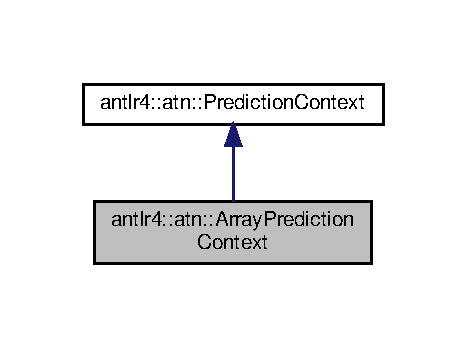
\includegraphics[width=224pt]{classantlr4_1_1atn_1_1ArrayPredictionContext__inherit__graph}
\end{center}
\end{figure}


Collaboration diagram for antlr4\+:\+:atn\+:\+:Array\+Prediction\+Context\+:
\nopagebreak
\begin{figure}[H]
\begin{center}
\leavevmode
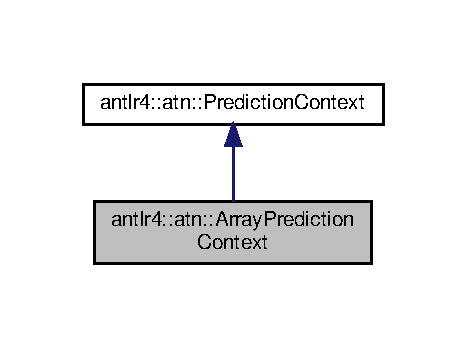
\includegraphics[width=224pt]{classantlr4_1_1atn_1_1ArrayPredictionContext__coll__graph}
\end{center}
\end{figure}
\subsection*{Public Member Functions}
\begin{DoxyCompactItemize}
\item 
\mbox{\Hypertarget{classantlr4_1_1atn_1_1ArrayPredictionContext_aeca230e73c888171d0fc31039df4eee7}\label{classantlr4_1_1atn_1_1ArrayPredictionContext_aeca230e73c888171d0fc31039df4eee7}} 
{\bfseries Array\+Prediction\+Context} (Ref$<$ \hyperlink{classantlr4_1_1atn_1_1SingletonPredictionContext}{Singleton\+Prediction\+Context} $>$ const \&a)
\item 
\mbox{\Hypertarget{classantlr4_1_1atn_1_1ArrayPredictionContext_a2ee2b2e07f1dd9dbcbfce902a092cd75}\label{classantlr4_1_1atn_1_1ArrayPredictionContext_a2ee2b2e07f1dd9dbcbfce902a092cd75}} 
{\bfseries Array\+Prediction\+Context} (std\+::vector$<$ Ref$<$ \hyperlink{classantlr4_1_1atn_1_1PredictionContext}{Prediction\+Context} $>$$>$ const \&parents\+\_\+, std\+::vector$<$ size\+\_\+t $>$ const \&\hyperlink{classantlr4_1_1atn_1_1ArrayPredictionContext_a40497e962ffa3f1d97695061b8222997}{return\+States})
\item 
\mbox{\Hypertarget{classantlr4_1_1atn_1_1ArrayPredictionContext_af2b9b082a447b8c00ebb0a99e7ca194d}\label{classantlr4_1_1atn_1_1ArrayPredictionContext_af2b9b082a447b8c00ebb0a99e7ca194d}} 
virtual bool \hyperlink{classantlr4_1_1atn_1_1ArrayPredictionContext_af2b9b082a447b8c00ebb0a99e7ca194d}{is\+Empty} () const override
\begin{DoxyCompactList}\small\item\em This means only the E\+M\+P\+TY (wildcard? not sure) context is in set. \end{DoxyCompactList}\item 
\mbox{\Hypertarget{classantlr4_1_1atn_1_1ArrayPredictionContext_a43a67555978f04529235e9221ddda067}\label{classantlr4_1_1atn_1_1ArrayPredictionContext_a43a67555978f04529235e9221ddda067}} 
virtual size\+\_\+t {\bfseries size} () const override
\item 
\mbox{\Hypertarget{classantlr4_1_1atn_1_1ArrayPredictionContext_a88a7a39151383ce08981056483f97724}\label{classantlr4_1_1atn_1_1ArrayPredictionContext_a88a7a39151383ce08981056483f97724}} 
virtual Ref$<$ \hyperlink{classantlr4_1_1atn_1_1PredictionContext}{Prediction\+Context} $>$ {\bfseries get\+Parent} (size\+\_\+t index) const override
\item 
\mbox{\Hypertarget{classantlr4_1_1atn_1_1ArrayPredictionContext_a9480cef9dfc74e5b8372c4c7f60c4c16}\label{classantlr4_1_1atn_1_1ArrayPredictionContext_a9480cef9dfc74e5b8372c4c7f60c4c16}} 
virtual size\+\_\+t {\bfseries get\+Return\+State} (size\+\_\+t index) const override
\item 
\mbox{\Hypertarget{classantlr4_1_1atn_1_1ArrayPredictionContext_abcdd5f5a1acc5ad7a6ff4a1ac488995d}\label{classantlr4_1_1atn_1_1ArrayPredictionContext_abcdd5f5a1acc5ad7a6ff4a1ac488995d}} 
bool {\bfseries operator==} (const \hyperlink{classantlr4_1_1atn_1_1PredictionContext}{Prediction\+Context} \&o) const override
\item 
\mbox{\Hypertarget{classantlr4_1_1atn_1_1ArrayPredictionContext_a76ba67a026cb2865a1516ceed4c88cbc}\label{classantlr4_1_1atn_1_1ArrayPredictionContext_a76ba67a026cb2865a1516ceed4c88cbc}} 
virtual std\+::string {\bfseries to\+String} () const override
\end{DoxyCompactItemize}
\subsection*{Public Attributes}
\begin{DoxyCompactItemize}
\item 
const std\+::vector$<$ Ref$<$ \hyperlink{classantlr4_1_1atn_1_1PredictionContext}{Prediction\+Context} $>$ $>$ \hyperlink{classantlr4_1_1atn_1_1ArrayPredictionContext_a97599e83122a8facd80d0747382e0201}{parents}
\item 
\mbox{\Hypertarget{classantlr4_1_1atn_1_1ArrayPredictionContext_a40497e962ffa3f1d97695061b8222997}\label{classantlr4_1_1atn_1_1ArrayPredictionContext_a40497e962ffa3f1d97695061b8222997}} 
const std\+::vector$<$ size\+\_\+t $>$ \hyperlink{classantlr4_1_1atn_1_1ArrayPredictionContext_a40497e962ffa3f1d97695061b8222997}{return\+States}
\begin{DoxyCompactList}\small\item\em Sorted for merge, no duplicates; if present, E\+M\+P\+T\+Y\+\_\+\+R\+E\+T\+U\+R\+N\+\_\+\+S\+T\+A\+TE is always last. \end{DoxyCompactList}\end{DoxyCompactItemize}
\subsection*{Additional Inherited Members}


\subsection{Member Data Documentation}
\mbox{\Hypertarget{classantlr4_1_1atn_1_1ArrayPredictionContext_a97599e83122a8facd80d0747382e0201}\label{classantlr4_1_1atn_1_1ArrayPredictionContext_a97599e83122a8facd80d0747382e0201}} 
\index{antlr4\+::atn\+::\+Array\+Prediction\+Context@{antlr4\+::atn\+::\+Array\+Prediction\+Context}!parents@{parents}}
\index{parents@{parents}!antlr4\+::atn\+::\+Array\+Prediction\+Context@{antlr4\+::atn\+::\+Array\+Prediction\+Context}}
\subsubsection{\texorpdfstring{parents}{parents}}
{\footnotesize\ttfamily const std\+::vector$<$Ref$<$\hyperlink{classantlr4_1_1atn_1_1PredictionContext}{Prediction\+Context}$>$ $>$ antlr4\+::atn\+::\+Array\+Prediction\+Context\+::parents}

Parent can be empty only if full ctx mode and we make an array from E\+M\+P\+TY and non-\/empty. We merge E\+M\+P\+TY by using null parent and return\+State == E\+M\+P\+T\+Y\+\_\+\+R\+E\+T\+U\+R\+N\+\_\+\+S\+T\+A\+TE. 

The documentation for this class was generated from the following files\+:\begin{DoxyCompactItemize}
\item 
atn/Array\+Prediction\+Context.\+h\item 
atn/Array\+Prediction\+Context.\+cpp\end{DoxyCompactItemize}

\hypertarget{classantlrcpp_1_1Arrays}{}\section{antlrcpp\+:\+:Arrays Class Reference}
\label{classantlrcpp_1_1Arrays}\index{antlrcpp\+::\+Arrays@{antlrcpp\+::\+Arrays}}
\subsection*{Public Member Functions}
\begin{DoxyCompactItemize}
\item 
\mbox{\Hypertarget{classantlrcpp_1_1Arrays_a7c34152170f8af54195d58b22b556f80}\label{classantlrcpp_1_1Arrays_a7c34152170f8af54195d58b22b556f80}} 
{\footnotesize template$<$$>$ }\\std\+::string {\bfseries to\+String} (const std\+::vector$<$ \hyperlink{classantlr4_1_1tree_1_1ParseTree}{antlr4\+::tree\+::\+Parse\+Tree} $\ast$$>$ \&source)
\end{DoxyCompactItemize}
\subsection*{Static Public Member Functions}
\begin{DoxyCompactItemize}
\item 
\mbox{\Hypertarget{classantlrcpp_1_1Arrays_a26206255ced012b39abd6038a26ebe52}\label{classantlrcpp_1_1Arrays_a26206255ced012b39abd6038a26ebe52}} 
static std\+::string {\bfseries list\+To\+String} (const std\+::vector$<$ std\+::string $>$ \&list, const std\+::string \&separator)
\item 
\mbox{\Hypertarget{classantlrcpp_1_1Arrays_a4c9ad217a86ea72ff6002d047a52b5b8}\label{classantlrcpp_1_1Arrays_a4c9ad217a86ea72ff6002d047a52b5b8}} 
{\footnotesize template$<$typename T $>$ }\\static bool {\bfseries equals} (const std\+::vector$<$ T $>$ \&a, const std\+::vector$<$ T $>$ \&b)
\item 
\mbox{\Hypertarget{classantlrcpp_1_1Arrays_a0a37625104accd974460c3bf0a2fb2e4}\label{classantlrcpp_1_1Arrays_a0a37625104accd974460c3bf0a2fb2e4}} 
{\footnotesize template$<$typename T $>$ }\\static bool {\bfseries equals} (const std\+::vector$<$ T $\ast$$>$ \&a, const std\+::vector$<$ T $\ast$$>$ \&b)
\item 
\mbox{\Hypertarget{classantlrcpp_1_1Arrays_a741eca4e255c0e2fbe1da6d61142373d}\label{classantlrcpp_1_1Arrays_a741eca4e255c0e2fbe1da6d61142373d}} 
{\footnotesize template$<$typename T $>$ }\\static bool {\bfseries equals} (const std\+::vector$<$ Ref$<$ T $>$$>$ \&a, const std\+::vector$<$ Ref$<$ T $>$$>$ \&b)
\item 
\mbox{\Hypertarget{classantlrcpp_1_1Arrays_a83ee6616704317f7c4ada54c734bd9d7}\label{classantlrcpp_1_1Arrays_a83ee6616704317f7c4ada54c734bd9d7}} 
{\footnotesize template$<$typename T $>$ }\\static std\+::string {\bfseries to\+String} (const std\+::vector$<$ T $>$ \&source)
\item 
\mbox{\Hypertarget{classantlrcpp_1_1Arrays_a85f05d02ce37da59147c1506f336c5d8}\label{classantlrcpp_1_1Arrays_a85f05d02ce37da59147c1506f336c5d8}} 
{\footnotesize template$<$typename T $>$ }\\static std\+::string {\bfseries to\+String} (const std\+::vector$<$ Ref$<$ T $>$$>$ \&source)
\item 
\mbox{\Hypertarget{classantlrcpp_1_1Arrays_ad1d931e19e30aa99e0044600970c63c4}\label{classantlrcpp_1_1Arrays_ad1d931e19e30aa99e0044600970c63c4}} 
{\footnotesize template$<$typename T $>$ }\\static std\+::string {\bfseries to\+String} (const std\+::vector$<$ T $\ast$$>$ \&source)
\end{DoxyCompactItemize}


The documentation for this class was generated from the following files\+:\begin{DoxyCompactItemize}
\item 
support/Arrays.\+h\item 
support/Arrays.\+cpp\end{DoxyCompactItemize}

\hypertarget{classantlr4_1_1atn_1_1ATNConfig}{}\section{antlr4\+:\+:atn\+:\+:A\+T\+N\+Config Class Reference}
\label{classantlr4_1_1atn_1_1ATNConfig}\index{antlr4\+::atn\+::\+A\+T\+N\+Config@{antlr4\+::atn\+::\+A\+T\+N\+Config}}


A tuple\+: (A\+TN state, predicted alt, syntactic, semantic context). The syntactic context is a graph-\/structured stack node whose path(s) to the root is the rule invocation(s) chain used to arrive at the state. The semantic context is the tree of semantic predicates encountered before reaching an A\+TN state.  




{\ttfamily \#include $<$A\+T\+N\+Config.\+h$>$}



Inheritance diagram for antlr4\+:\+:atn\+:\+:A\+T\+N\+Config\+:
\nopagebreak
\begin{figure}[H]
\begin{center}
\leavevmode
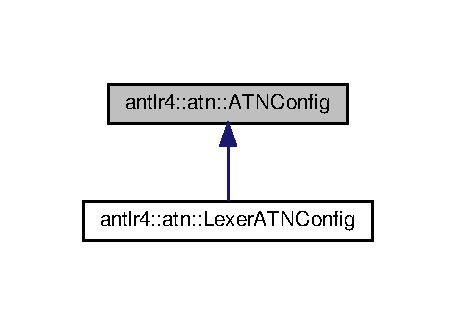
\includegraphics[width=219pt]{classantlr4_1_1atn_1_1ATNConfig__inherit__graph}
\end{center}
\end{figure}
\subsection*{Classes}
\begin{DoxyCompactItemize}
\item 
struct \hyperlink{structantlr4_1_1atn_1_1ATNConfig_1_1Comparer}{Comparer}
\item 
struct \hyperlink{structantlr4_1_1atn_1_1ATNConfig_1_1Hasher}{Hasher}
\end{DoxyCompactItemize}
\subsection*{Public Types}
\begin{DoxyCompactItemize}
\item 
\mbox{\Hypertarget{classantlr4_1_1atn_1_1ATNConfig_a8b8a460058db3442824bc69cec6ed54b}\label{classantlr4_1_1atn_1_1ATNConfig_a8b8a460058db3442824bc69cec6ed54b}} 
using {\bfseries Set} = std\+::unordered\+\_\+set$<$ Ref$<$ \hyperlink{classantlr4_1_1atn_1_1ATNConfig}{A\+T\+N\+Config} $>$, \hyperlink{structantlr4_1_1atn_1_1ATNConfig_1_1Hasher}{Hasher}, \hyperlink{structantlr4_1_1atn_1_1ATNConfig_1_1Comparer}{Comparer} $>$
\end{DoxyCompactItemize}
\subsection*{Public Member Functions}
\begin{DoxyCompactItemize}
\item 
\mbox{\Hypertarget{classantlr4_1_1atn_1_1ATNConfig_a65120d9eeb1ca13f5cd2ad2c866aaf04}\label{classantlr4_1_1atn_1_1ATNConfig_a65120d9eeb1ca13f5cd2ad2c866aaf04}} 
{\bfseries A\+T\+N\+Config} (A\+T\+N\+State $\ast$\hyperlink{classantlr4_1_1atn_1_1ATNConfig_ae2e2757839f60f245b1a30c1f83bd52d}{state}, size\+\_\+t \hyperlink{classantlr4_1_1atn_1_1ATNConfig_ab4b68e6c1b1c70197a21fd62009bf9b8}{alt}, Ref$<$ \hyperlink{classantlr4_1_1atn_1_1PredictionContext}{Prediction\+Context} $>$ const \&\hyperlink{classantlr4_1_1atn_1_1ATNConfig_a1f30878a632f67672f16b52eefb01f26}{context})
\item 
\mbox{\Hypertarget{classantlr4_1_1atn_1_1ATNConfig_ac54395dc00b5c04f084af66a2ed3b735}\label{classantlr4_1_1atn_1_1ATNConfig_ac54395dc00b5c04f084af66a2ed3b735}} 
{\bfseries A\+T\+N\+Config} (A\+T\+N\+State $\ast$\hyperlink{classantlr4_1_1atn_1_1ATNConfig_ae2e2757839f60f245b1a30c1f83bd52d}{state}, size\+\_\+t \hyperlink{classantlr4_1_1atn_1_1ATNConfig_ab4b68e6c1b1c70197a21fd62009bf9b8}{alt}, Ref$<$ \hyperlink{classantlr4_1_1atn_1_1PredictionContext}{Prediction\+Context} $>$ const \&\hyperlink{classantlr4_1_1atn_1_1ATNConfig_a1f30878a632f67672f16b52eefb01f26}{context}, Ref$<$ \hyperlink{classantlr4_1_1atn_1_1SemanticContext}{Semantic\+Context} $>$ const \&\hyperlink{classantlr4_1_1atn_1_1ATNConfig_a99d4da95eab2009d3f0605aa8c051092}{semantic\+Context})
\item 
\mbox{\Hypertarget{classantlr4_1_1atn_1_1ATNConfig_a0e1a16490805abc6e4b0aeed02ab490f}\label{classantlr4_1_1atn_1_1ATNConfig_a0e1a16490805abc6e4b0aeed02ab490f}} 
{\bfseries A\+T\+N\+Config} (Ref$<$ \hyperlink{classantlr4_1_1atn_1_1ATNConfig}{A\+T\+N\+Config} $>$ const \&c)
\item 
\mbox{\Hypertarget{classantlr4_1_1atn_1_1ATNConfig_a0728c2f08b7082fbb96af203d1fc4fe6}\label{classantlr4_1_1atn_1_1ATNConfig_a0728c2f08b7082fbb96af203d1fc4fe6}} 
{\bfseries A\+T\+N\+Config} (Ref$<$ \hyperlink{classantlr4_1_1atn_1_1ATNConfig}{A\+T\+N\+Config} $>$ const \&c, A\+T\+N\+State $\ast$\hyperlink{classantlr4_1_1atn_1_1ATNConfig_ae2e2757839f60f245b1a30c1f83bd52d}{state})
\item 
\mbox{\Hypertarget{classantlr4_1_1atn_1_1ATNConfig_ae6f62fccacc7f596ec7363e1a214b441}\label{classantlr4_1_1atn_1_1ATNConfig_ae6f62fccacc7f596ec7363e1a214b441}} 
{\bfseries A\+T\+N\+Config} (Ref$<$ \hyperlink{classantlr4_1_1atn_1_1ATNConfig}{A\+T\+N\+Config} $>$ const \&c, A\+T\+N\+State $\ast$\hyperlink{classantlr4_1_1atn_1_1ATNConfig_ae2e2757839f60f245b1a30c1f83bd52d}{state}, Ref$<$ \hyperlink{classantlr4_1_1atn_1_1SemanticContext}{Semantic\+Context} $>$ const \&\hyperlink{classantlr4_1_1atn_1_1ATNConfig_a99d4da95eab2009d3f0605aa8c051092}{semantic\+Context})
\item 
\mbox{\Hypertarget{classantlr4_1_1atn_1_1ATNConfig_a2fd76ca1075bf19dc9785559816ed66c}\label{classantlr4_1_1atn_1_1ATNConfig_a2fd76ca1075bf19dc9785559816ed66c}} 
{\bfseries A\+T\+N\+Config} (Ref$<$ \hyperlink{classantlr4_1_1atn_1_1ATNConfig}{A\+T\+N\+Config} $>$ const \&c, Ref$<$ \hyperlink{classantlr4_1_1atn_1_1SemanticContext}{Semantic\+Context} $>$ const \&\hyperlink{classantlr4_1_1atn_1_1ATNConfig_a99d4da95eab2009d3f0605aa8c051092}{semantic\+Context})
\item 
\mbox{\Hypertarget{classantlr4_1_1atn_1_1ATNConfig_af728088ce35d2b674223ca6a064ee32f}\label{classantlr4_1_1atn_1_1ATNConfig_af728088ce35d2b674223ca6a064ee32f}} 
{\bfseries A\+T\+N\+Config} (Ref$<$ \hyperlink{classantlr4_1_1atn_1_1ATNConfig}{A\+T\+N\+Config} $>$ const \&c, A\+T\+N\+State $\ast$\hyperlink{classantlr4_1_1atn_1_1ATNConfig_ae2e2757839f60f245b1a30c1f83bd52d}{state}, Ref$<$ \hyperlink{classantlr4_1_1atn_1_1PredictionContext}{Prediction\+Context} $>$ const \&\hyperlink{classantlr4_1_1atn_1_1ATNConfig_a1f30878a632f67672f16b52eefb01f26}{context})
\item 
\mbox{\Hypertarget{classantlr4_1_1atn_1_1ATNConfig_abdb202bbb0a83139927915c04de72e30}\label{classantlr4_1_1atn_1_1ATNConfig_abdb202bbb0a83139927915c04de72e30}} 
{\bfseries A\+T\+N\+Config} (Ref$<$ \hyperlink{classantlr4_1_1atn_1_1ATNConfig}{A\+T\+N\+Config} $>$ const \&c, A\+T\+N\+State $\ast$\hyperlink{classantlr4_1_1atn_1_1ATNConfig_ae2e2757839f60f245b1a30c1f83bd52d}{state}, Ref$<$ \hyperlink{classantlr4_1_1atn_1_1PredictionContext}{Prediction\+Context} $>$ const \&\hyperlink{classantlr4_1_1atn_1_1ATNConfig_a1f30878a632f67672f16b52eefb01f26}{context}, Ref$<$ \hyperlink{classantlr4_1_1atn_1_1SemanticContext}{Semantic\+Context} $>$ const \&\hyperlink{classantlr4_1_1atn_1_1ATNConfig_a99d4da95eab2009d3f0605aa8c051092}{semantic\+Context})
\item 
\mbox{\Hypertarget{classantlr4_1_1atn_1_1ATNConfig_a562b69b9d973c3526223298273d0eaff}\label{classantlr4_1_1atn_1_1ATNConfig_a562b69b9d973c3526223298273d0eaff}} 
{\bfseries A\+T\+N\+Config} (\hyperlink{classantlr4_1_1atn_1_1ATNConfig}{A\+T\+N\+Config} const \&)=default
\item 
\mbox{\Hypertarget{classantlr4_1_1atn_1_1ATNConfig_adb35bccb780fcbf21bbc7f444b0d57db}\label{classantlr4_1_1atn_1_1ATNConfig_adb35bccb780fcbf21bbc7f444b0d57db}} 
\hyperlink{classantlr4_1_1atn_1_1ATNConfig}{A\+T\+N\+Config} \& {\bfseries operator=} (\hyperlink{classantlr4_1_1atn_1_1ATNConfig}{A\+T\+N\+Config} const \&)=default
\item 
\mbox{\Hypertarget{classantlr4_1_1atn_1_1ATNConfig_a54366241b4eab72f182ce26e6b9d55fb}\label{classantlr4_1_1atn_1_1ATNConfig_a54366241b4eab72f182ce26e6b9d55fb}} 
virtual size\+\_\+t {\bfseries hash\+Code} () const
\item 
size\+\_\+t \hyperlink{classantlr4_1_1atn_1_1ATNConfig_ad06261312a72cfeb52a351a77c7bbb86}{get\+Outer\+Context\+Depth} () const
\item 
\mbox{\Hypertarget{classantlr4_1_1atn_1_1ATNConfig_a2cd2c3806345787f3d3af9b4ca11ee93}\label{classantlr4_1_1atn_1_1ATNConfig_a2cd2c3806345787f3d3af9b4ca11ee93}} 
bool {\bfseries is\+Precedence\+Filter\+Suppressed} () const
\item 
\mbox{\Hypertarget{classantlr4_1_1atn_1_1ATNConfig_a28317105ace986bdf348e0cdbade81e9}\label{classantlr4_1_1atn_1_1ATNConfig_a28317105ace986bdf348e0cdbade81e9}} 
void {\bfseries set\+Precedence\+Filter\+Suppressed} (bool value)
\item 
bool \hyperlink{classantlr4_1_1atn_1_1ATNConfig_a3ec70b1cc06793d2b9d5aab1e662909b}{operator==} (const \hyperlink{classantlr4_1_1atn_1_1ATNConfig}{A\+T\+N\+Config} \&other) const
\item 
\mbox{\Hypertarget{classantlr4_1_1atn_1_1ATNConfig_afa411b4b9765a9040f0ccbf2b7d7dbce}\label{classantlr4_1_1atn_1_1ATNConfig_afa411b4b9765a9040f0ccbf2b7d7dbce}} 
bool {\bfseries operator!=} (const \hyperlink{classantlr4_1_1atn_1_1ATNConfig}{A\+T\+N\+Config} \&other) const
\item 
\mbox{\Hypertarget{classantlr4_1_1atn_1_1ATNConfig_afd8ea6c2122f79c898968f6dbae6697f}\label{classantlr4_1_1atn_1_1ATNConfig_afd8ea6c2122f79c898968f6dbae6697f}} 
virtual std\+::string {\bfseries to\+String} ()
\item 
\mbox{\Hypertarget{classantlr4_1_1atn_1_1ATNConfig_a2358f792cada9677c439169e5cf643a4}\label{classantlr4_1_1atn_1_1ATNConfig_a2358f792cada9677c439169e5cf643a4}} 
std\+::string {\bfseries to\+String} (bool show\+Alt)
\end{DoxyCompactItemize}
\subsection*{Public Attributes}
\begin{DoxyCompactItemize}
\item 
\mbox{\Hypertarget{classantlr4_1_1atn_1_1ATNConfig_ae2e2757839f60f245b1a30c1f83bd52d}\label{classantlr4_1_1atn_1_1ATNConfig_ae2e2757839f60f245b1a30c1f83bd52d}} 
A\+T\+N\+State $\ast$ \hyperlink{classantlr4_1_1atn_1_1ATNConfig_ae2e2757839f60f245b1a30c1f83bd52d}{state}
\begin{DoxyCompactList}\small\item\em The A\+TN state associated with this configuration. \end{DoxyCompactList}\item 
\mbox{\Hypertarget{classantlr4_1_1atn_1_1ATNConfig_ab4b68e6c1b1c70197a21fd62009bf9b8}\label{classantlr4_1_1atn_1_1ATNConfig_ab4b68e6c1b1c70197a21fd62009bf9b8}} 
const size\+\_\+t \hyperlink{classantlr4_1_1atn_1_1ATNConfig_ab4b68e6c1b1c70197a21fd62009bf9b8}{alt}
\begin{DoxyCompactList}\small\item\em What alt (or lexer rule) is predicted by this configuration. \end{DoxyCompactList}\item 
Ref$<$ \hyperlink{classantlr4_1_1atn_1_1PredictionContext}{Prediction\+Context} $>$ \hyperlink{classantlr4_1_1atn_1_1ATNConfig_a1f30878a632f67672f16b52eefb01f26}{context}
\item 
size\+\_\+t \hyperlink{classantlr4_1_1atn_1_1ATNConfig_a3dda5924725f5c1cb7d798dea4b4fca7}{reaches\+Into\+Outer\+Context}
\item 
\mbox{\Hypertarget{classantlr4_1_1atn_1_1ATNConfig_a99d4da95eab2009d3f0605aa8c051092}\label{classantlr4_1_1atn_1_1ATNConfig_a99d4da95eab2009d3f0605aa8c051092}} 
Ref$<$ \hyperlink{classantlr4_1_1atn_1_1SemanticContext}{Semantic\+Context} $>$ \hyperlink{classantlr4_1_1atn_1_1ATNConfig_a99d4da95eab2009d3f0605aa8c051092}{semantic\+Context}
\begin{DoxyCompactList}\small\item\em Can be shared between multiple \hyperlink{classantlr4_1_1atn_1_1ATNConfig}{A\+T\+N\+Config} instances. \end{DoxyCompactList}\end{DoxyCompactItemize}


\subsection{Detailed Description}
A tuple\+: (A\+TN state, predicted alt, syntactic, semantic context). The syntactic context is a graph-\/structured stack node whose path(s) to the root is the rule invocation(s) chain used to arrive at the state. The semantic context is the tree of semantic predicates encountered before reaching an A\+TN state. 



\subsection{Member Function Documentation}
\mbox{\Hypertarget{classantlr4_1_1atn_1_1ATNConfig_ad06261312a72cfeb52a351a77c7bbb86}\label{classantlr4_1_1atn_1_1ATNConfig_ad06261312a72cfeb52a351a77c7bbb86}} 
\index{antlr4\+::atn\+::\+A\+T\+N\+Config@{antlr4\+::atn\+::\+A\+T\+N\+Config}!get\+Outer\+Context\+Depth@{get\+Outer\+Context\+Depth}}
\index{get\+Outer\+Context\+Depth@{get\+Outer\+Context\+Depth}!antlr4\+::atn\+::\+A\+T\+N\+Config@{antlr4\+::atn\+::\+A\+T\+N\+Config}}
\subsubsection{\texorpdfstring{get\+Outer\+Context\+Depth()}{getOuterContextDepth()}}
{\footnotesize\ttfamily size\+\_\+t A\+T\+N\+Config\+::get\+Outer\+Context\+Depth (\begin{DoxyParamCaption}{ }\end{DoxyParamCaption}) const}

This method gets the value of the \hyperlink{classantlr4_1_1atn_1_1ATNConfig_a3dda5924725f5c1cb7d798dea4b4fca7}{reaches\+Into\+Outer\+Context} field as it existed prior to the introduction of the \hyperlink{}{is\+Precedence\+Filter\+Suppressed} method. \mbox{\Hypertarget{classantlr4_1_1atn_1_1ATNConfig_a3ec70b1cc06793d2b9d5aab1e662909b}\label{classantlr4_1_1atn_1_1ATNConfig_a3ec70b1cc06793d2b9d5aab1e662909b}} 
\index{antlr4\+::atn\+::\+A\+T\+N\+Config@{antlr4\+::atn\+::\+A\+T\+N\+Config}!operator==@{operator==}}
\index{operator==@{operator==}!antlr4\+::atn\+::\+A\+T\+N\+Config@{antlr4\+::atn\+::\+A\+T\+N\+Config}}
\subsubsection{\texorpdfstring{operator==()}{operator==()}}
{\footnotesize\ttfamily bool A\+T\+N\+Config\+::operator== (\begin{DoxyParamCaption}\item[{const \hyperlink{classantlr4_1_1atn_1_1ATNConfig}{A\+T\+N\+Config} \&}]{other }\end{DoxyParamCaption}) const}

An A\+TN configuration is equal to another if both have the same state, they predict the same alternative, and syntactic/semantic contexts are the same. 

\subsection{Member Data Documentation}
\mbox{\Hypertarget{classantlr4_1_1atn_1_1ATNConfig_a1f30878a632f67672f16b52eefb01f26}\label{classantlr4_1_1atn_1_1ATNConfig_a1f30878a632f67672f16b52eefb01f26}} 
\index{antlr4\+::atn\+::\+A\+T\+N\+Config@{antlr4\+::atn\+::\+A\+T\+N\+Config}!context@{context}}
\index{context@{context}!antlr4\+::atn\+::\+A\+T\+N\+Config@{antlr4\+::atn\+::\+A\+T\+N\+Config}}
\subsubsection{\texorpdfstring{context}{context}}
{\footnotesize\ttfamily Ref$<$\hyperlink{classantlr4_1_1atn_1_1PredictionContext}{Prediction\+Context}$>$ antlr4\+::atn\+::\+A\+T\+N\+Config\+::context}

The stack of invoking states leading to the rule/states associated with this config. We track only those contexts pushed during execution of the A\+TN simulator.

Can be shared between multiple A\+N\+T\+Config instances. \mbox{\Hypertarget{classantlr4_1_1atn_1_1ATNConfig_a3dda5924725f5c1cb7d798dea4b4fca7}\label{classantlr4_1_1atn_1_1ATNConfig_a3dda5924725f5c1cb7d798dea4b4fca7}} 
\index{antlr4\+::atn\+::\+A\+T\+N\+Config@{antlr4\+::atn\+::\+A\+T\+N\+Config}!reaches\+Into\+Outer\+Context@{reaches\+Into\+Outer\+Context}}
\index{reaches\+Into\+Outer\+Context@{reaches\+Into\+Outer\+Context}!antlr4\+::atn\+::\+A\+T\+N\+Config@{antlr4\+::atn\+::\+A\+T\+N\+Config}}
\subsubsection{\texorpdfstring{reaches\+Into\+Outer\+Context}{reachesIntoOuterContext}}
{\footnotesize\ttfamily size\+\_\+t antlr4\+::atn\+::\+A\+T\+N\+Config\+::reaches\+Into\+Outer\+Context}

We cannot execute predicates dependent upon local context unless we know for sure we are in the correct context. Because there is no way to do this efficiently, we simply cannot evaluate dependent predicates unless we are in the rule that initially invokes the A\+TN simulator.

closure() tracks the depth of how far we dip into the outer context\+: depth $>$ 0. Note that it may not be totally accurate depth since I don\textquotesingle{}t ever decrement. T\+O\+\_\+\+DO\+: make it a boolean then

For memory efficiency, the \hyperlink{}{is\+Precedence\+Filter\+Suppressed} method is also backed by this field. Since the field is publicly accessible, the highest bit which would not cause the value to become negative is used to store this field. This choice minimizes the risk that code which only compares this value to 0 would be affected by the new purpose of the flag. It also ensures the performance of the existing \hyperlink{classantlr4_1_1atn_1_1ATNConfig}{A\+T\+N\+Config} constructors as well as certain operations like \hyperlink{}{A\+T\+N\+Config\+Set\#add(\+A\+T\+N\+Config, Double\+Key\+Map)} method are {\itshape completely} unaffected by the change.

The documentation for this class was generated from the following files\+:\begin{DoxyCompactItemize}
\item 
atn/A\+T\+N\+Config.\+h\item 
atn/A\+T\+N\+Config.\+cpp\end{DoxyCompactItemize}

\hypertarget{classantlr4_1_1atn_1_1ATNConfigSet}{}\section{antlr4\+:\+:atn\+:\+:A\+T\+N\+Config\+Set Class Reference}
\label{classantlr4_1_1atn_1_1ATNConfigSet}\index{antlr4\+::atn\+::\+A\+T\+N\+Config\+Set@{antlr4\+::atn\+::\+A\+T\+N\+Config\+Set}}


{\ttfamily \#include $<$A\+T\+N\+Config\+Set.\+h$>$}



Inheritance diagram for antlr4\+:\+:atn\+:\+:A\+T\+N\+Config\+Set\+:
\nopagebreak
\begin{figure}[H]
\begin{center}
\leavevmode
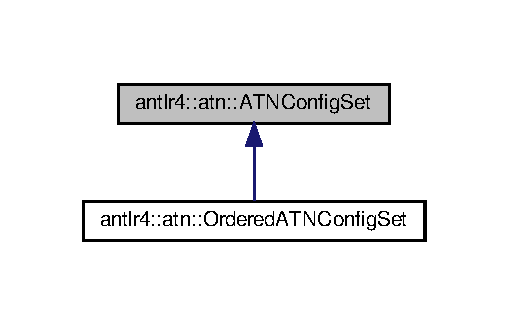
\includegraphics[width=244pt]{classantlr4_1_1atn_1_1ATNConfigSet__inherit__graph}
\end{center}
\end{figure}


Collaboration diagram for antlr4\+:\+:atn\+:\+:A\+T\+N\+Config\+Set\+:
\nopagebreak
\begin{figure}[H]
\begin{center}
\leavevmode
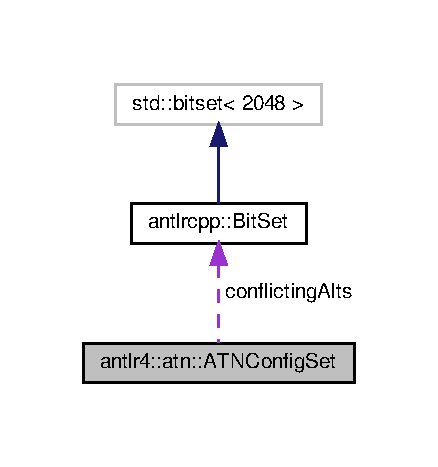
\includegraphics[width=210pt]{classantlr4_1_1atn_1_1ATNConfigSet__coll__graph}
\end{center}
\end{figure}
\subsection*{Public Member Functions}
\begin{DoxyCompactItemize}
\item 
\mbox{\Hypertarget{classantlr4_1_1atn_1_1ATNConfigSet_a69c297789ef198d08b6690587b74b44a}\label{classantlr4_1_1atn_1_1ATNConfigSet_a69c297789ef198d08b6690587b74b44a}} 
{\bfseries A\+T\+N\+Config\+Set} (bool \hyperlink{classantlr4_1_1atn_1_1ATNConfigSet_af5ef274bd4b6185f2865add7f943633c}{full\+Ctx}=true)
\item 
\mbox{\Hypertarget{classantlr4_1_1atn_1_1ATNConfigSet_a22c2e827ee70c41d4a6ef326e211ea4d}\label{classantlr4_1_1atn_1_1ATNConfigSet_a22c2e827ee70c41d4a6ef326e211ea4d}} 
{\bfseries A\+T\+N\+Config\+Set} (const Ref$<$ \hyperlink{classantlr4_1_1atn_1_1ATNConfigSet}{A\+T\+N\+Config\+Set} $>$ \&old)
\item 
\mbox{\Hypertarget{classantlr4_1_1atn_1_1ATNConfigSet_aa2fc9693c9586947a34877d179020f73}\label{classantlr4_1_1atn_1_1ATNConfigSet_aa2fc9693c9586947a34877d179020f73}} 
virtual bool {\bfseries add} (const Ref$<$ \hyperlink{classantlr4_1_1atn_1_1ATNConfig}{A\+T\+N\+Config} $>$ \&config)
\end{DoxyCompactItemize}
\subsection*{Public Attributes}
\begin{DoxyCompactItemize}
\item 
\mbox{\Hypertarget{classantlr4_1_1atn_1_1ATNConfigSet_a5404495afc6bb7823429d202a1625bdc}\label{classantlr4_1_1atn_1_1ATNConfigSet_a5404495afc6bb7823429d202a1625bdc}} 
std\+::vector$<$ Ref$<$ \hyperlink{classantlr4_1_1atn_1_1ATNConfig}{A\+T\+N\+Config} $>$ $>$ \hyperlink{classantlr4_1_1atn_1_1ATNConfigSet_a5404495afc6bb7823429d202a1625bdc}{configs}
\begin{DoxyCompactList}\small\item\em Track the elements as they are added to the set; supports get(i) \end{DoxyCompactList}\item 
\mbox{\Hypertarget{classantlr4_1_1atn_1_1ATNConfigSet_abbb020e6f64f01e7bd959551afb1fc93}\label{classantlr4_1_1atn_1_1ATNConfigSet_abbb020e6f64f01e7bd959551afb1fc93}} 
size\+\_\+t {\bfseries unique\+Alt}
\item 
\hyperlink{classantlrcpp_1_1BitSet}{antlrcpp\+::\+Bit\+Set} \hyperlink{classantlr4_1_1atn_1_1ATNConfigSet_a37b30c5a21147bdc63325cffd2f99041}{conflicting\+Alts}
\item 
\mbox{\Hypertarget{classantlr4_1_1atn_1_1ATNConfigSet_acf4dc336b07151064e0acdd84d5a6dcc}\label{classantlr4_1_1atn_1_1ATNConfigSet_acf4dc336b07151064e0acdd84d5a6dcc}} 
bool {\bfseries has\+Semantic\+Context}
\item 
\mbox{\Hypertarget{classantlr4_1_1atn_1_1ATNConfigSet_a8ed06e3a821509fe0f003c00e2a14676}\label{classantlr4_1_1atn_1_1ATNConfigSet_a8ed06e3a821509fe0f003c00e2a14676}} 
bool {\bfseries dips\+Into\+Outer\+Context}
\item 
const bool \hyperlink{classantlr4_1_1atn_1_1ATNConfigSet_af5ef274bd4b6185f2865add7f943633c}{full\+Ctx}
\end{DoxyCompactItemize}


\subsection{Detailed Description}
Specialized set that can track info about the set, with support for combining similar configurations using a graph-\/structured stack. 

\subsection{Member Data Documentation}
\mbox{\Hypertarget{classantlr4_1_1atn_1_1ATNConfigSet_a37b30c5a21147bdc63325cffd2f99041}\label{classantlr4_1_1atn_1_1ATNConfigSet_a37b30c5a21147bdc63325cffd2f99041}} 
\index{antlr4\+::atn\+::\+A\+T\+N\+Config\+Set@{antlr4\+::atn\+::\+A\+T\+N\+Config\+Set}!conflicting\+Alts@{conflicting\+Alts}}
\index{conflicting\+Alts@{conflicting\+Alts}!antlr4\+::atn\+::\+A\+T\+N\+Config\+Set@{antlr4\+::atn\+::\+A\+T\+N\+Config\+Set}}
\subsubsection{\texorpdfstring{conflicting\+Alts}{conflictingAlts}}
{\footnotesize\ttfamily \hyperlink{classantlrcpp_1_1BitSet}{antlrcpp\+::\+Bit\+Set} antlr4\+::atn\+::\+A\+T\+N\+Config\+Set\+::conflicting\+Alts}

Currently this is only used when we detect S\+LL conflict; this does not necessarily represent the ambiguous alternatives. In fact, I should also point out that this seems to include predicated alternatives that have predicates that evaluate to false. Computed in compute\+Target\+State(). \mbox{\Hypertarget{classantlr4_1_1atn_1_1ATNConfigSet_af5ef274bd4b6185f2865add7f943633c}\label{classantlr4_1_1atn_1_1ATNConfigSet_af5ef274bd4b6185f2865add7f943633c}} 
\index{antlr4\+::atn\+::\+A\+T\+N\+Config\+Set@{antlr4\+::atn\+::\+A\+T\+N\+Config\+Set}!full\+Ctx@{full\+Ctx}}
\index{full\+Ctx@{full\+Ctx}!antlr4\+::atn\+::\+A\+T\+N\+Config\+Set@{antlr4\+::atn\+::\+A\+T\+N\+Config\+Set}}
\subsubsection{\texorpdfstring{full\+Ctx}{fullCtx}}
{\footnotesize\ttfamily const bool antlr4\+::atn\+::\+A\+T\+N\+Config\+Set\+::full\+Ctx}

Indicates that this configuration set is part of a full context LL prediction. It will be used to determine how to merge \$. With S\+LL it\textquotesingle{}s a wildcard whereas it is not for LL context merge. 

The documentation for this class was generated from the following files\+:\begin{DoxyCompactItemize}
\item 
atn/A\+T\+N\+Config\+Set.\+h\item 
atn/A\+T\+N\+Config\+Set.\+cpp\end{DoxyCompactItemize}

\hypertarget{classantlr4_1_1atn_1_1ATNDeserializationOptions}{}\section{antlr4\+:\+:atn\+:\+:A\+T\+N\+Deserialization\+Options Class Reference}
\label{classantlr4_1_1atn_1_1ATNDeserializationOptions}\index{antlr4\+::atn\+::\+A\+T\+N\+Deserialization\+Options@{antlr4\+::atn\+::\+A\+T\+N\+Deserialization\+Options}}
\subsection*{Public Member Functions}
\begin{DoxyCompactItemize}
\item 
\mbox{\Hypertarget{classantlr4_1_1atn_1_1ATNDeserializationOptions_a6de965a7e58ea8c013a6f34e7d566252}\label{classantlr4_1_1atn_1_1ATNDeserializationOptions_a6de965a7e58ea8c013a6f34e7d566252}} 
{\bfseries A\+T\+N\+Deserialization\+Options} (\hyperlink{classantlr4_1_1atn_1_1ATNDeserializationOptions}{A\+T\+N\+Deserialization\+Options} $\ast$options)
\item 
\mbox{\Hypertarget{classantlr4_1_1atn_1_1ATNDeserializationOptions_ad0afe636bf23a3c7c8e4bd8db78c0a93}\label{classantlr4_1_1atn_1_1ATNDeserializationOptions_ad0afe636bf23a3c7c8e4bd8db78c0a93}} 
{\bfseries A\+T\+N\+Deserialization\+Options} (\hyperlink{classantlr4_1_1atn_1_1ATNDeserializationOptions}{A\+T\+N\+Deserialization\+Options} const \&)=default
\item 
\mbox{\Hypertarget{classantlr4_1_1atn_1_1ATNDeserializationOptions_a28535f48c323880c4ad9f3b4edc0ecce}\label{classantlr4_1_1atn_1_1ATNDeserializationOptions_a28535f48c323880c4ad9f3b4edc0ecce}} 
\hyperlink{classantlr4_1_1atn_1_1ATNDeserializationOptions}{A\+T\+N\+Deserialization\+Options} \& {\bfseries operator=} (\hyperlink{classantlr4_1_1atn_1_1ATNDeserializationOptions}{A\+T\+N\+Deserialization\+Options} const \&)=default
\item 
\mbox{\Hypertarget{classantlr4_1_1atn_1_1ATNDeserializationOptions_a43b2b980a1926142a0b40405b8356f1a}\label{classantlr4_1_1atn_1_1ATNDeserializationOptions_a43b2b980a1926142a0b40405b8356f1a}} 
bool {\bfseries is\+Read\+Only} ()
\item 
\mbox{\Hypertarget{classantlr4_1_1atn_1_1ATNDeserializationOptions_af5dd63a76ab916c4f0328c7e9cca9094}\label{classantlr4_1_1atn_1_1ATNDeserializationOptions_af5dd63a76ab916c4f0328c7e9cca9094}} 
void {\bfseries make\+Read\+Only} ()
\item 
\mbox{\Hypertarget{classantlr4_1_1atn_1_1ATNDeserializationOptions_ab4a9cd8654e425f266825520c0b96588}\label{classantlr4_1_1atn_1_1ATNDeserializationOptions_ab4a9cd8654e425f266825520c0b96588}} 
bool {\bfseries is\+Verify\+A\+TN} ()
\item 
\mbox{\Hypertarget{classantlr4_1_1atn_1_1ATNDeserializationOptions_ae323852fdeb297428519eaa69d7cb1c8}\label{classantlr4_1_1atn_1_1ATNDeserializationOptions_ae323852fdeb297428519eaa69d7cb1c8}} 
void {\bfseries set\+Verify\+A\+TN} (bool verify)
\item 
\mbox{\Hypertarget{classantlr4_1_1atn_1_1ATNDeserializationOptions_a828a11936772939844686dfc7d879da2}\label{classantlr4_1_1atn_1_1ATNDeserializationOptions_a828a11936772939844686dfc7d879da2}} 
bool {\bfseries is\+Generate\+Rule\+Bypass\+Transitions} ()
\item 
\mbox{\Hypertarget{classantlr4_1_1atn_1_1ATNDeserializationOptions_aa6af4f41c9ec5990c04c03bf5db790ea}\label{classantlr4_1_1atn_1_1ATNDeserializationOptions_aa6af4f41c9ec5990c04c03bf5db790ea}} 
void {\bfseries set\+Generate\+Rule\+Bypass\+Transitions} (bool generate)
\end{DoxyCompactItemize}
\subsection*{Static Public Member Functions}
\begin{DoxyCompactItemize}
\item 
\mbox{\Hypertarget{classantlr4_1_1atn_1_1ATNDeserializationOptions_a045ca6e8199ccfc8df2deb0b8d4decc2}\label{classantlr4_1_1atn_1_1ATNDeserializationOptions_a045ca6e8199ccfc8df2deb0b8d4decc2}} 
static const \hyperlink{classantlr4_1_1atn_1_1ATNDeserializationOptions}{A\+T\+N\+Deserialization\+Options} \& {\bfseries get\+Default\+Options} ()
\end{DoxyCompactItemize}
\subsection*{Protected Member Functions}
\begin{DoxyCompactItemize}
\item 
\mbox{\Hypertarget{classantlr4_1_1atn_1_1ATNDeserializationOptions_ad94e6e8dad3c194181af4a59969e0ca4}\label{classantlr4_1_1atn_1_1ATNDeserializationOptions_ad94e6e8dad3c194181af4a59969e0ca4}} 
virtual void {\bfseries throw\+If\+Read\+Only} ()
\end{DoxyCompactItemize}


The documentation for this class was generated from the following files\+:\begin{DoxyCompactItemize}
\item 
atn/A\+T\+N\+Deserialization\+Options.\+h\item 
atn/A\+T\+N\+Deserialization\+Options.\+cpp\end{DoxyCompactItemize}

\hypertarget{classantlr4_1_1atn_1_1ATNDeserializer}{}\section{antlr4\+:\+:atn\+:\+:A\+T\+N\+Deserializer Class Reference}
\label{classantlr4_1_1atn_1_1ATNDeserializer}\index{antlr4\+::atn\+::\+A\+T\+N\+Deserializer@{antlr4\+::atn\+::\+A\+T\+N\+Deserializer}}
\subsection*{Public Member Functions}
\begin{DoxyCompactItemize}
\item 
\mbox{\Hypertarget{classantlr4_1_1atn_1_1ATNDeserializer_a948f22aa8f3aad8fd65c1a6d8838bc47}\label{classantlr4_1_1atn_1_1ATNDeserializer_a948f22aa8f3aad8fd65c1a6d8838bc47}} 
{\bfseries A\+T\+N\+Deserializer} (const \hyperlink{classantlr4_1_1atn_1_1ATNDeserializationOptions}{A\+T\+N\+Deserialization\+Options} \&dso)
\item 
\mbox{\Hypertarget{classantlr4_1_1atn_1_1ATNDeserializer_aefd9354c6031246ae9d09a2bba89cb47}\label{classantlr4_1_1atn_1_1ATNDeserializer_aefd9354c6031246ae9d09a2bba89cb47}} 
virtual A\+TN {\bfseries deserialize} (const std\+::vector$<$ uint16\+\_\+t $>$ \&input)
\item 
\mbox{\Hypertarget{classantlr4_1_1atn_1_1ATNDeserializer_a57391bf3e7694c08de4d29db2a69129c}\label{classantlr4_1_1atn_1_1ATNDeserializer_a57391bf3e7694c08de4d29db2a69129c}} 
virtual void {\bfseries verify\+A\+TN} (const A\+TN \&atn)
\end{DoxyCompactItemize}
\subsection*{Static Public Member Functions}
\begin{DoxyCompactItemize}
\item 
\mbox{\Hypertarget{classantlr4_1_1atn_1_1ATNDeserializer_a00524eaade634ca63a4c5fe3d65a9b75}\label{classantlr4_1_1atn_1_1ATNDeserializer_a00524eaade634ca63a4c5fe3d65a9b75}} 
static \hyperlink{classGuid}{Guid} \hyperlink{classantlr4_1_1atn_1_1ATNDeserializer_a00524eaade634ca63a4c5fe3d65a9b75}{S\+E\+R\+I\+A\+L\+I\+Z\+E\+D\+\_\+\+U\+U\+ID} ()
\begin{DoxyCompactList}\small\item\em This is the current serialized U\+U\+ID. \end{DoxyCompactList}\item 
\mbox{\Hypertarget{classantlr4_1_1atn_1_1ATNDeserializer_aa995f4f04abbad84a72ede0aa2affbdb}\label{classantlr4_1_1atn_1_1ATNDeserializer_aa995f4f04abbad84a72ede0aa2affbdb}} 
static \hyperlink{classGuid}{Guid} {\bfseries to\+U\+U\+ID} (const unsigned short $\ast$data, size\+\_\+t offset)
\item 
\mbox{\Hypertarget{classantlr4_1_1atn_1_1ATNDeserializer_acc8c93e4b176da3869d143f1e01960cc}\label{classantlr4_1_1atn_1_1ATNDeserializer_acc8c93e4b176da3869d143f1e01960cc}} 
static void {\bfseries check\+Condition} (bool condition)
\item 
\mbox{\Hypertarget{classantlr4_1_1atn_1_1ATNDeserializer_acbc323b929a3afac1a4dffbda33dca6b}\label{classantlr4_1_1atn_1_1ATNDeserializer_acbc323b929a3afac1a4dffbda33dca6b}} 
static void {\bfseries check\+Condition} (bool condition, const std\+::string \&message)
\item 
\mbox{\Hypertarget{classantlr4_1_1atn_1_1ATNDeserializer_a42f8e8a738438bb7320be3e0db340fea}\label{classantlr4_1_1atn_1_1ATNDeserializer_a42f8e8a738438bb7320be3e0db340fea}} 
static \hyperlink{classantlr4_1_1atn_1_1Transition}{Transition} $\ast$ {\bfseries edge\+Factory} (const A\+TN \&atn, size\+\_\+t type, size\+\_\+t src, size\+\_\+t trg, size\+\_\+t arg1, size\+\_\+t arg2, size\+\_\+t arg3, const std\+::vector$<$ \hyperlink{classantlr4_1_1misc_1_1IntervalSet}{misc\+::\+Interval\+Set} $>$ \&sets)
\item 
\mbox{\Hypertarget{classantlr4_1_1atn_1_1ATNDeserializer_a1942c23ca9c2b004374dfcf55f8a5bb3}\label{classantlr4_1_1atn_1_1ATNDeserializer_a1942c23ca9c2b004374dfcf55f8a5bb3}} 
static A\+T\+N\+State $\ast$ {\bfseries state\+Factory} (size\+\_\+t type, size\+\_\+t rule\+Index)
\end{DoxyCompactItemize}
\subsection*{Static Public Attributes}
\begin{DoxyCompactItemize}
\item 
\mbox{\Hypertarget{classantlr4_1_1atn_1_1ATNDeserializer_a4160c21d7e3ee10c751a97ddad05697a}\label{classantlr4_1_1atn_1_1ATNDeserializer_a4160c21d7e3ee10c751a97ddad05697a}} 
static const size\+\_\+t {\bfseries S\+E\+R\+I\+A\+L\+I\+Z\+E\+D\+\_\+\+V\+E\+R\+S\+I\+ON} = 3
\end{DoxyCompactItemize}


The documentation for this class was generated from the following files\+:\begin{DoxyCompactItemize}
\item 
atn/A\+T\+N\+Deserializer.\+h\item 
atn/A\+T\+N\+Deserializer.\+cpp\end{DoxyCompactItemize}

\hypertarget{classantlr4_1_1atn_1_1ATNSerializer}{}\section{antlr4\+:\+:atn\+:\+:A\+T\+N\+Serializer Class Reference}
\label{classantlr4_1_1atn_1_1ATNSerializer}\index{antlr4\+::atn\+::\+A\+T\+N\+Serializer@{antlr4\+::atn\+::\+A\+T\+N\+Serializer}}
\subsection*{Public Member Functions}
\begin{DoxyCompactItemize}
\item 
\mbox{\Hypertarget{classantlr4_1_1atn_1_1ATNSerializer_a75bff3cf4e62ff43bfdedd1795f9fad8}\label{classantlr4_1_1atn_1_1ATNSerializer_a75bff3cf4e62ff43bfdedd1795f9fad8}} 
{\bfseries A\+T\+N\+Serializer} (A\+TN $\ast$atn)
\item 
\mbox{\Hypertarget{classantlr4_1_1atn_1_1ATNSerializer_a17b466a6c4cf5e9e44224b8a245f7231}\label{classantlr4_1_1atn_1_1ATNSerializer_a17b466a6c4cf5e9e44224b8a245f7231}} 
{\bfseries A\+T\+N\+Serializer} (A\+TN $\ast$atn, const std\+::vector$<$ std\+::string $>$ \&token\+Names)
\item 
virtual std\+::vector$<$ size\+\_\+t $>$ \hyperlink{classantlr4_1_1atn_1_1ATNSerializer_ae4d16b888446eddfd0faaf5356d6d884}{serialize} ()
\begin{DoxyCompactList}\small\item\em Serialize state descriptors, edge descriptors, and decision-\/$>$state map into list of ints\+: \end{DoxyCompactList}\item 
\mbox{\Hypertarget{classantlr4_1_1atn_1_1ATNSerializer_a938398654ea3ca5d26699dce55785600}\label{classantlr4_1_1atn_1_1ATNSerializer_a938398654ea3ca5d26699dce55785600}} 
virtual std\+::string {\bfseries decode} (const std\+::wstring \&data)
\item 
\mbox{\Hypertarget{classantlr4_1_1atn_1_1ATNSerializer_a90abb185836850e7d17be3e94109b45b}\label{classantlr4_1_1atn_1_1ATNSerializer_a90abb185836850e7d17be3e94109b45b}} 
virtual std\+::string {\bfseries get\+Token\+Name} (size\+\_\+t t)
\end{DoxyCompactItemize}
\subsection*{Static Public Member Functions}
\begin{DoxyCompactItemize}
\item 
\mbox{\Hypertarget{classantlr4_1_1atn_1_1ATNSerializer_a837138e7a36404f8397569f95e4e98bc}\label{classantlr4_1_1atn_1_1ATNSerializer_a837138e7a36404f8397569f95e4e98bc}} 
static std\+::wstring \hyperlink{classantlr4_1_1atn_1_1ATNSerializer_a837138e7a36404f8397569f95e4e98bc}{get\+Serialized\+As\+String} (A\+TN $\ast$atn)
\begin{DoxyCompactList}\small\item\em Used by Java target to encode short/int array as chars in string. \end{DoxyCompactList}\item 
\mbox{\Hypertarget{classantlr4_1_1atn_1_1ATNSerializer_acc79fa1515109ef7edbb54278fdbb1a9}\label{classantlr4_1_1atn_1_1ATNSerializer_acc79fa1515109ef7edbb54278fdbb1a9}} 
static std\+::vector$<$ size\+\_\+t $>$ {\bfseries get\+Serialized} (A\+TN $\ast$atn)
\item 
\mbox{\Hypertarget{classantlr4_1_1atn_1_1ATNSerializer_a9664559456e4c5babc1a6f650a1bbcb7}\label{classantlr4_1_1atn_1_1ATNSerializer_a9664559456e4c5babc1a6f650a1bbcb7}} 
static std\+::string {\bfseries get\+Decoded} (A\+TN $\ast$atn, std\+::vector$<$ std\+::string $>$ \&token\+Names)
\end{DoxyCompactItemize}
\subsection*{Public Attributes}
\begin{DoxyCompactItemize}
\item 
\mbox{\Hypertarget{classantlr4_1_1atn_1_1ATNSerializer_a8d94c9a858d576727244bbe896fe52c7}\label{classantlr4_1_1atn_1_1ATNSerializer_a8d94c9a858d576727244bbe896fe52c7}} 
A\+TN $\ast$ {\bfseries atn}
\end{DoxyCompactItemize}


\subsection{Member Function Documentation}
\mbox{\Hypertarget{classantlr4_1_1atn_1_1ATNSerializer_ae4d16b888446eddfd0faaf5356d6d884}\label{classantlr4_1_1atn_1_1ATNSerializer_ae4d16b888446eddfd0faaf5356d6d884}} 
\index{antlr4\+::atn\+::\+A\+T\+N\+Serializer@{antlr4\+::atn\+::\+A\+T\+N\+Serializer}!serialize@{serialize}}
\index{serialize@{serialize}!antlr4\+::atn\+::\+A\+T\+N\+Serializer@{antlr4\+::atn\+::\+A\+T\+N\+Serializer}}
\subsubsection{\texorpdfstring{serialize()}{serialize()}}
{\footnotesize\ttfamily std\+::vector$<$ size\+\_\+t $>$ A\+T\+N\+Serializer\+::serialize (\begin{DoxyParamCaption}{ }\end{DoxyParamCaption})\hspace{0.3cm}{\ttfamily [virtual]}}



Serialize state descriptors, edge descriptors, and decision-\/$>$state map into list of ints\+: 

grammar-\/type, (A\+N\+T\+L\+R\+Parser.\+L\+E\+X\+ER, ...) max token type, num states, state-\/0-\/type rule\+Index, state-\/1-\/type rule\+Index, ... state-\/i-\/type rule\+Index optional-\/arg ... num rules, rule-\/1-\/start-\/state rule-\/1-\/args, rule-\/2-\/start-\/state rule-\/2-\/args, ... (args are token type,action\+Index in lexer else 0,0) num modes, mode-\/0-\/start-\/state, mode-\/1-\/start-\/state, ... (parser has 0 modes) num sets set-\/0-\/interval-\/count intervals, set-\/1-\/interval-\/count intervals, ... num total edges, src, trg, edge-\/type, edge arg1, optional edge arg2 (present always), ... num decisions, decision-\/0-\/start-\/state, decision-\/1-\/start-\/state, ...

Convenient to pack into unsigned shorts to make as Java string. 

The documentation for this class was generated from the following files\+:\begin{DoxyCompactItemize}
\item 
atn/A\+T\+N\+Serializer.\+h\item 
atn/A\+T\+N\+Serializer.\+cpp\end{DoxyCompactItemize}

\hypertarget{classantlr4_1_1atn_1_1ATNSimulator}{}\section{antlr4\+:\+:atn\+:\+:A\+T\+N\+Simulator Class Reference}
\label{classantlr4_1_1atn_1_1ATNSimulator}\index{antlr4\+::atn\+::\+A\+T\+N\+Simulator@{antlr4\+::atn\+::\+A\+T\+N\+Simulator}}


Inheritance diagram for antlr4\+:\+:atn\+:\+:A\+T\+N\+Simulator\+:
\nopagebreak
\begin{figure}[H]
\begin{center}
\leavevmode
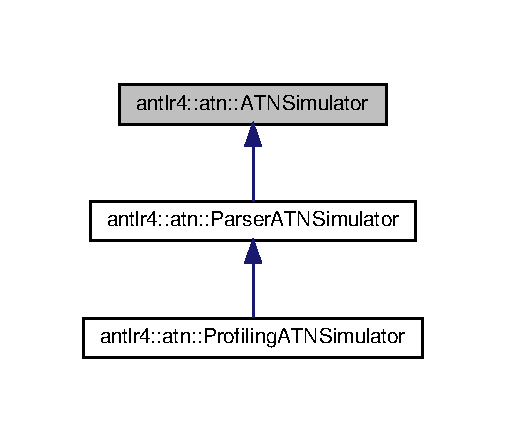
\includegraphics[width=243pt]{classantlr4_1_1atn_1_1ATNSimulator__inherit__graph}
\end{center}
\end{figure}


Collaboration diagram for antlr4\+:\+:atn\+:\+:A\+T\+N\+Simulator\+:
\nopagebreak
\begin{figure}[H]
\begin{center}
\leavevmode
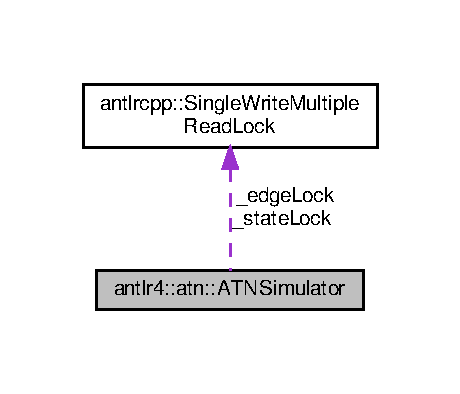
\includegraphics[width=221pt]{classantlr4_1_1atn_1_1ATNSimulator__coll__graph}
\end{center}
\end{figure}
\subsection*{Public Member Functions}
\begin{DoxyCompactItemize}
\item 
\mbox{\Hypertarget{classantlr4_1_1atn_1_1ATNSimulator_aea00369023c5b32d3b73e9e4b2726cbe}\label{classantlr4_1_1atn_1_1ATNSimulator_aea00369023c5b32d3b73e9e4b2726cbe}} 
{\bfseries A\+T\+N\+Simulator} (const A\+TN \&atn, Prediction\+Context\+Cache \&shared\+Context\+Cache)
\item 
\mbox{\Hypertarget{classantlr4_1_1atn_1_1ATNSimulator_a282a76fb17fd8529c48e695b4dc5134c}\label{classantlr4_1_1atn_1_1ATNSimulator_a282a76fb17fd8529c48e695b4dc5134c}} 
virtual void {\bfseries reset} ()=0
\item 
virtual void \hyperlink{classantlr4_1_1atn_1_1ATNSimulator_a3358fa3e8ebcb4abeeceb914b0b07f10}{clear\+D\+FA} ()
\item 
\mbox{\Hypertarget{classantlr4_1_1atn_1_1ATNSimulator_a112cafa9554cff202c037672ddc918e5}\label{classantlr4_1_1atn_1_1ATNSimulator_a112cafa9554cff202c037672ddc918e5}} 
virtual Prediction\+Context\+Cache \& {\bfseries get\+Shared\+Context\+Cache} ()
\item 
\mbox{\Hypertarget{classantlr4_1_1atn_1_1ATNSimulator_aa4fb144eaf79bf6052a0abe290f7a3a2}\label{classantlr4_1_1atn_1_1ATNSimulator_aa4fb144eaf79bf6052a0abe290f7a3a2}} 
virtual Ref$<$ \hyperlink{classantlr4_1_1atn_1_1PredictionContext}{Prediction\+Context} $>$ {\bfseries get\+Cached\+Context} (Ref$<$ \hyperlink{classantlr4_1_1atn_1_1PredictionContext}{Prediction\+Context} $>$ const \&context)
\end{DoxyCompactItemize}
\subsection*{Static Public Member Functions}
\begin{DoxyCompactItemize}
\item 
static A\+TN \hyperlink{classantlr4_1_1atn_1_1ATNSimulator_ae516df637ee1f4be4787d533ed88b3b9}{deserialize} (const std\+::vector$<$ uint16\+\_\+t $>$ \&data)
\item 
static void \hyperlink{classantlr4_1_1atn_1_1ATNSimulator_aa827be017f3bf3a431ef91972d38e3d1}{check\+Condition} (bool condition)
\item 
static void \hyperlink{classantlr4_1_1atn_1_1ATNSimulator_a394cdeb1e2d6028bc73e0f1d22830b3d}{check\+Condition} (bool condition, const std\+::string \&message)
\item 
static \hyperlink{classantlr4_1_1atn_1_1Transition}{Transition} $\ast$ \hyperlink{classantlr4_1_1atn_1_1ATNSimulator_a8e3fc8caefaecf90ac5eb45561aafdcc}{edge\+Factory} (const A\+TN \&atn, int type, int src, int trg, int arg1, int arg2, int arg3, const std\+::vector$<$ \hyperlink{classantlr4_1_1misc_1_1IntervalSet}{misc\+::\+Interval\+Set} $>$ \&sets)
\item 
static A\+T\+N\+State $\ast$ \hyperlink{classantlr4_1_1atn_1_1ATNSimulator_a57878604b6496cc6aa80e29811e05660}{state\+Factory} (int type, int rule\+Index)
\end{DoxyCompactItemize}
\subsection*{Public Attributes}
\begin{DoxyCompactItemize}
\item 
\mbox{\Hypertarget{classantlr4_1_1atn_1_1ATNSimulator_afec8e232a4c11c864ecc770252a2bcb6}\label{classantlr4_1_1atn_1_1ATNSimulator_afec8e232a4c11c864ecc770252a2bcb6}} 
const A\+TN \& {\bfseries atn}
\end{DoxyCompactItemize}
\subsection*{Static Public Attributes}
\begin{DoxyCompactItemize}
\item 
\mbox{\Hypertarget{classantlr4_1_1atn_1_1ATNSimulator_a1a88e9a52986711b319268c6e6faf6c6}\label{classantlr4_1_1atn_1_1ATNSimulator_a1a88e9a52986711b319268c6e6faf6c6}} 
static const Ref$<$ dfa\+::\+D\+F\+A\+State $>$ \hyperlink{classantlr4_1_1atn_1_1ATNSimulator_a1a88e9a52986711b319268c6e6faf6c6}{E\+R\+R\+OR} = std\+::make\+\_\+shared$<$D\+F\+A\+State$>$(I\+N\+T32\+\_\+\+M\+AX)
\begin{DoxyCompactList}\small\item\em Must distinguish between missing edge and edge we know leads nowhere. \end{DoxyCompactList}\end{DoxyCompactItemize}
\subsection*{Protected Attributes}
\begin{DoxyCompactItemize}
\item 
Prediction\+Context\+Cache \& \hyperlink{classantlr4_1_1atn_1_1ATNSimulator_a73bf77d58d1457cc0543600da3201bea}{\+\_\+shared\+Context\+Cache}
\begin{DoxyCompactList}\small\item\em The context cache maps all \hyperlink{classantlr4_1_1atn_1_1PredictionContext}{Prediction\+Context} objects that are equals() to a single cached copy. This cache is shared across all contexts in all A\+T\+N\+Configs in all D\+FA states. We rebuild each \hyperlink{classantlr4_1_1atn_1_1ATNConfigSet}{A\+T\+N\+Config\+Set} to use only cached nodes/graphs in add\+D\+F\+A\+State(). We don\textquotesingle{}t want to fill this during closure() since there are lots of contexts that pop up but are not used ever again. It also greatly slows down closure(). 

This cache makes a huge difference in memory and a little bit in speed. For the Java grammar on java.$\ast$, it dropped the memory requirements at the end from 25M to 16M. We don\textquotesingle{}t store any of the full context graphs in the D\+FA because they are limited to local context only, but apparently there\textquotesingle{}s a lot of repetition there as well. We optimize the config contexts before storing the config set in the D\+FA states by literally rebuilding them with cached subgraphs only. 

I tried a cache for use during closure operations, that was whacked after each adaptive\+Predict(). It cost a little bit more time I think and doesn\textquotesingle{}t save on the overall footprint so it\textquotesingle{}s not worth the complexity. \end{DoxyCompactList}\end{DoxyCompactItemize}
\subsection*{Static Protected Attributes}
\begin{DoxyCompactItemize}
\item 
\mbox{\Hypertarget{classantlr4_1_1atn_1_1ATNSimulator_a0ceff3caefbd8f9067c549fdf60e973b}\label{classantlr4_1_1atn_1_1ATNSimulator_a0ceff3caefbd8f9067c549fdf60e973b}} 
static \hyperlink{classantlrcpp_1_1SingleWriteMultipleReadLock}{antlrcpp\+::\+Single\+Write\+Multiple\+Read\+Lock} {\bfseries \+\_\+state\+Lock}
\item 
\mbox{\Hypertarget{classantlr4_1_1atn_1_1ATNSimulator_ab3c0921267abe8227f51aa4f1201a82a}\label{classantlr4_1_1atn_1_1ATNSimulator_ab3c0921267abe8227f51aa4f1201a82a}} 
static \hyperlink{classantlrcpp_1_1SingleWriteMultipleReadLock}{antlrcpp\+::\+Single\+Write\+Multiple\+Read\+Lock} {\bfseries \+\_\+edge\+Lock}
\end{DoxyCompactItemize}


\subsection{Member Function Documentation}
\mbox{\Hypertarget{classantlr4_1_1atn_1_1ATNSimulator_aa827be017f3bf3a431ef91972d38e3d1}\label{classantlr4_1_1atn_1_1ATNSimulator_aa827be017f3bf3a431ef91972d38e3d1}} 
\index{antlr4\+::atn\+::\+A\+T\+N\+Simulator@{antlr4\+::atn\+::\+A\+T\+N\+Simulator}!check\+Condition@{check\+Condition}}
\index{check\+Condition@{check\+Condition}!antlr4\+::atn\+::\+A\+T\+N\+Simulator@{antlr4\+::atn\+::\+A\+T\+N\+Simulator}}
\subsubsection{\texorpdfstring{check\+Condition()}{checkCondition()}\hspace{0.1cm}{\footnotesize\ttfamily [1/2]}}
{\footnotesize\ttfamily void A\+T\+N\+Simulator\+::check\+Condition (\begin{DoxyParamCaption}\item[{bool}]{condition }\end{DoxyParamCaption})\hspace{0.3cm}{\ttfamily [static]}}

\begin{DoxyRefDesc}{Deprecated}
\item[\hyperlink{deprecated__deprecated000002}{Deprecated}]Use \begin{DoxySeeAlso}{See also}
A\+T\+N\+Deserializer\+::check\+Condition(boolean)


\end{DoxySeeAlso}
instead. \end{DoxyRefDesc}
\mbox{\Hypertarget{classantlr4_1_1atn_1_1ATNSimulator_a394cdeb1e2d6028bc73e0f1d22830b3d}\label{classantlr4_1_1atn_1_1ATNSimulator_a394cdeb1e2d6028bc73e0f1d22830b3d}} 
\index{antlr4\+::atn\+::\+A\+T\+N\+Simulator@{antlr4\+::atn\+::\+A\+T\+N\+Simulator}!check\+Condition@{check\+Condition}}
\index{check\+Condition@{check\+Condition}!antlr4\+::atn\+::\+A\+T\+N\+Simulator@{antlr4\+::atn\+::\+A\+T\+N\+Simulator}}
\subsubsection{\texorpdfstring{check\+Condition()}{checkCondition()}\hspace{0.1cm}{\footnotesize\ttfamily [2/2]}}
{\footnotesize\ttfamily void A\+T\+N\+Simulator\+::check\+Condition (\begin{DoxyParamCaption}\item[{bool}]{condition,  }\item[{const std\+::string \&}]{message }\end{DoxyParamCaption})\hspace{0.3cm}{\ttfamily [static]}}

\begin{DoxyRefDesc}{Deprecated}
\item[\hyperlink{deprecated__deprecated000003}{Deprecated}]Use \begin{DoxySeeAlso}{See also}
A\+T\+N\+Deserializer\+::check\+Condition(boolean, String)


\end{DoxySeeAlso}
instead. \end{DoxyRefDesc}
\mbox{\Hypertarget{classantlr4_1_1atn_1_1ATNSimulator_a3358fa3e8ebcb4abeeceb914b0b07f10}\label{classantlr4_1_1atn_1_1ATNSimulator_a3358fa3e8ebcb4abeeceb914b0b07f10}} 
\index{antlr4\+::atn\+::\+A\+T\+N\+Simulator@{antlr4\+::atn\+::\+A\+T\+N\+Simulator}!clear\+D\+FA@{clear\+D\+FA}}
\index{clear\+D\+FA@{clear\+D\+FA}!antlr4\+::atn\+::\+A\+T\+N\+Simulator@{antlr4\+::atn\+::\+A\+T\+N\+Simulator}}
\subsubsection{\texorpdfstring{clear\+D\+F\+A()}{clearDFA()}}
{\footnotesize\ttfamily void A\+T\+N\+Simulator\+::clear\+D\+FA (\begin{DoxyParamCaption}{ }\end{DoxyParamCaption})\hspace{0.3cm}{\ttfamily [virtual]}}

Clear the D\+FA cache used by the current instance. Since the D\+FA cache may be shared by multiple A\+TN simulators, this method may affect the performance (but not accuracy) of other parsers which are being used concurrently.


\begin{DoxyExceptions}{Exceptions}
{\em \hyperlink{classantlr4_1_1UnsupportedOperationException}{Unsupported\+Operation\+Exception}} & if the current instance does not support clearing the D\+FA.\\
\hline
\end{DoxyExceptions}
\begin{DoxySince}{Since}
4.\+3 
\end{DoxySince}


Reimplemented in \hyperlink{classantlr4_1_1atn_1_1ParserATNSimulator_a846da7dc607b212d443cb401f5830bae}{antlr4\+::atn\+::\+Parser\+A\+T\+N\+Simulator}.

\mbox{\Hypertarget{classantlr4_1_1atn_1_1ATNSimulator_ae516df637ee1f4be4787d533ed88b3b9}\label{classantlr4_1_1atn_1_1ATNSimulator_ae516df637ee1f4be4787d533ed88b3b9}} 
\index{antlr4\+::atn\+::\+A\+T\+N\+Simulator@{antlr4\+::atn\+::\+A\+T\+N\+Simulator}!deserialize@{deserialize}}
\index{deserialize@{deserialize}!antlr4\+::atn\+::\+A\+T\+N\+Simulator@{antlr4\+::atn\+::\+A\+T\+N\+Simulator}}
\subsubsection{\texorpdfstring{deserialize()}{deserialize()}}
{\footnotesize\ttfamily A\+TN A\+T\+N\+Simulator\+::deserialize (\begin{DoxyParamCaption}\item[{const std\+::vector$<$ uint16\+\_\+t $>$ \&}]{data }\end{DoxyParamCaption})\hspace{0.3cm}{\ttfamily [static]}}

\begin{DoxyRefDesc}{Deprecated}
\item[\hyperlink{deprecated__deprecated000001}{Deprecated}]Use \begin{DoxySeeAlso}{See also}
A\+T\+N\+Deserializer\+::deserialize


\end{DoxySeeAlso}
instead. \end{DoxyRefDesc}
\mbox{\Hypertarget{classantlr4_1_1atn_1_1ATNSimulator_a8e3fc8caefaecf90ac5eb45561aafdcc}\label{classantlr4_1_1atn_1_1ATNSimulator_a8e3fc8caefaecf90ac5eb45561aafdcc}} 
\index{antlr4\+::atn\+::\+A\+T\+N\+Simulator@{antlr4\+::atn\+::\+A\+T\+N\+Simulator}!edge\+Factory@{edge\+Factory}}
\index{edge\+Factory@{edge\+Factory}!antlr4\+::atn\+::\+A\+T\+N\+Simulator@{antlr4\+::atn\+::\+A\+T\+N\+Simulator}}
\subsubsection{\texorpdfstring{edge\+Factory()}{edgeFactory()}}
{\footnotesize\ttfamily \hyperlink{classantlr4_1_1atn_1_1Transition}{Transition} $\ast$ A\+T\+N\+Simulator\+::edge\+Factory (\begin{DoxyParamCaption}\item[{const A\+TN \&}]{atn,  }\item[{int}]{type,  }\item[{int}]{src,  }\item[{int}]{trg,  }\item[{int}]{arg1,  }\item[{int}]{arg2,  }\item[{int}]{arg3,  }\item[{const std\+::vector$<$ \hyperlink{classantlr4_1_1misc_1_1IntervalSet}{misc\+::\+Interval\+Set} $>$ \&}]{sets }\end{DoxyParamCaption})\hspace{0.3cm}{\ttfamily [static]}}

\begin{DoxyRefDesc}{Deprecated}
\item[\hyperlink{deprecated__deprecated000004}{Deprecated}]Use \begin{DoxySeeAlso}{See also}
A\+T\+N\+Deserializer\+::edge\+Factory


\end{DoxySeeAlso}
instead. \end{DoxyRefDesc}
\mbox{\Hypertarget{classantlr4_1_1atn_1_1ATNSimulator_a57878604b6496cc6aa80e29811e05660}\label{classantlr4_1_1atn_1_1ATNSimulator_a57878604b6496cc6aa80e29811e05660}} 
\index{antlr4\+::atn\+::\+A\+T\+N\+Simulator@{antlr4\+::atn\+::\+A\+T\+N\+Simulator}!state\+Factory@{state\+Factory}}
\index{state\+Factory@{state\+Factory}!antlr4\+::atn\+::\+A\+T\+N\+Simulator@{antlr4\+::atn\+::\+A\+T\+N\+Simulator}}
\subsubsection{\texorpdfstring{state\+Factory()}{stateFactory()}}
{\footnotesize\ttfamily A\+T\+N\+State $\ast$ A\+T\+N\+Simulator\+::state\+Factory (\begin{DoxyParamCaption}\item[{int}]{type,  }\item[{int}]{rule\+Index }\end{DoxyParamCaption})\hspace{0.3cm}{\ttfamily [static]}}

\begin{DoxyRefDesc}{Deprecated}
\item[\hyperlink{deprecated__deprecated000005}{Deprecated}]Use \begin{DoxySeeAlso}{See also}
A\+T\+N\+Deserializer\+::state\+Factory


\end{DoxySeeAlso}
instead. \end{DoxyRefDesc}


\subsection{Member Data Documentation}
\mbox{\Hypertarget{classantlr4_1_1atn_1_1ATNSimulator_a73bf77d58d1457cc0543600da3201bea}\label{classantlr4_1_1atn_1_1ATNSimulator_a73bf77d58d1457cc0543600da3201bea}} 
\index{antlr4\+::atn\+::\+A\+T\+N\+Simulator@{antlr4\+::atn\+::\+A\+T\+N\+Simulator}!\+\_\+shared\+Context\+Cache@{\+\_\+shared\+Context\+Cache}}
\index{\+\_\+shared\+Context\+Cache@{\+\_\+shared\+Context\+Cache}!antlr4\+::atn\+::\+A\+T\+N\+Simulator@{antlr4\+::atn\+::\+A\+T\+N\+Simulator}}
\subsubsection{\texorpdfstring{\+\_\+shared\+Context\+Cache}{\_sharedContextCache}}
{\footnotesize\ttfamily Prediction\+Context\+Cache\& antlr4\+::atn\+::\+A\+T\+N\+Simulator\+::\+\_\+shared\+Context\+Cache\hspace{0.3cm}{\ttfamily [protected]}}



The context cache maps all \hyperlink{classantlr4_1_1atn_1_1PredictionContext}{Prediction\+Context} objects that are equals() to a single cached copy. This cache is shared across all contexts in all A\+T\+N\+Configs in all D\+FA states. We rebuild each \hyperlink{classantlr4_1_1atn_1_1ATNConfigSet}{A\+T\+N\+Config\+Set} to use only cached nodes/graphs in add\+D\+F\+A\+State(). We don\textquotesingle{}t want to fill this during closure() since there are lots of contexts that pop up but are not used ever again. It also greatly slows down closure(). 

This cache makes a huge difference in memory and a little bit in speed. For the Java grammar on java.$\ast$, it dropped the memory requirements at the end from 25M to 16M. We don\textquotesingle{}t store any of the full context graphs in the D\+FA because they are limited to local context only, but apparently there\textquotesingle{}s a lot of repetition there as well. We optimize the config contexts before storing the config set in the D\+FA states by literally rebuilding them with cached subgraphs only. 

I tried a cache for use during closure operations, that was whacked after each adaptive\+Predict(). It cost a little bit more time I think and doesn\textquotesingle{}t save on the overall footprint so it\textquotesingle{}s not worth the complexity. 



The documentation for this class was generated from the following files\+:\begin{DoxyCompactItemize}
\item 
atn/A\+T\+N\+Simulator.\+h\item 
atn/A\+T\+N\+Simulator.\+cpp\end{DoxyCompactItemize}

\hypertarget{classantlr4_1_1atn_1_1AtomTransition}{}\section{antlr4\+:\+:atn\+:\+:Atom\+Transition Class Reference}
\label{classantlr4_1_1atn_1_1AtomTransition}\index{antlr4\+::atn\+::\+Atom\+Transition@{antlr4\+::atn\+::\+Atom\+Transition}}


T\+O\+\_\+\+DO\+: make all transitions sets? no, should remove set edges.  




{\ttfamily \#include $<$Atom\+Transition.\+h$>$}



Inheritance diagram for antlr4\+:\+:atn\+:\+:Atom\+Transition\+:
\nopagebreak
\begin{figure}[H]
\begin{center}
\leavevmode
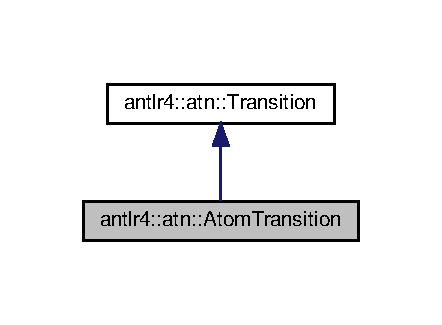
\includegraphics[width=212pt]{classantlr4_1_1atn_1_1AtomTransition__inherit__graph}
\end{center}
\end{figure}


Collaboration diagram for antlr4\+:\+:atn\+:\+:Atom\+Transition\+:
\nopagebreak
\begin{figure}[H]
\begin{center}
\leavevmode
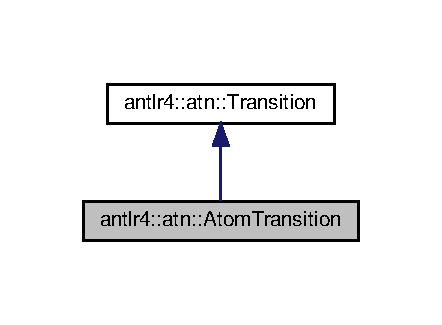
\includegraphics[width=212pt]{classantlr4_1_1atn_1_1AtomTransition__coll__graph}
\end{center}
\end{figure}
\subsection*{Public Member Functions}
\begin{DoxyCompactItemize}
\item 
\mbox{\Hypertarget{classantlr4_1_1atn_1_1AtomTransition_af69d81cfb163080e0c98b620b8cb66a7}\label{classantlr4_1_1atn_1_1AtomTransition_af69d81cfb163080e0c98b620b8cb66a7}} 
{\bfseries Atom\+Transition} (A\+T\+N\+State $\ast$\hyperlink{classantlr4_1_1atn_1_1Transition_aaaed7f4ddda71e156b36de33e88f66a7}{target}, size\+\_\+t label)
\item 
\mbox{\Hypertarget{classantlr4_1_1atn_1_1AtomTransition_aa02c1811edfef1f09fe06e3310e7c1f5}\label{classantlr4_1_1atn_1_1AtomTransition_aa02c1811edfef1f09fe06e3310e7c1f5}} 
virtual Serialization\+Type {\bfseries get\+Serialization\+Type} () const override
\item 
\mbox{\Hypertarget{classantlr4_1_1atn_1_1AtomTransition_aa9a089ea07ee3667d4c2b8a9c9b1637e}\label{classantlr4_1_1atn_1_1AtomTransition_aa9a089ea07ee3667d4c2b8a9c9b1637e}} 
virtual \hyperlink{classantlr4_1_1misc_1_1IntervalSet}{misc\+::\+Interval\+Set} {\bfseries label} () const override
\item 
\mbox{\Hypertarget{classantlr4_1_1atn_1_1AtomTransition_aceb4171c2bb81125de577e2c84c82778}\label{classantlr4_1_1atn_1_1AtomTransition_aceb4171c2bb81125de577e2c84c82778}} 
virtual bool {\bfseries matches} (size\+\_\+t symbol, size\+\_\+t min\+Vocab\+Symbol, size\+\_\+t max\+Vocab\+Symbol) const override
\item 
\mbox{\Hypertarget{classantlr4_1_1atn_1_1AtomTransition_a2d9e71455e1ebfb9f878cb5dfa92ed96}\label{classantlr4_1_1atn_1_1AtomTransition_a2d9e71455e1ebfb9f878cb5dfa92ed96}} 
virtual std\+::string {\bfseries to\+String} () const override
\end{DoxyCompactItemize}
\subsection*{Public Attributes}
\begin{DoxyCompactItemize}
\item 
\mbox{\Hypertarget{classantlr4_1_1atn_1_1AtomTransition_ac793fab5323d347fe2b7c159c9b9c556}\label{classantlr4_1_1atn_1_1AtomTransition_ac793fab5323d347fe2b7c159c9b9c556}} 
const size\+\_\+t \hyperlink{classantlr4_1_1atn_1_1AtomTransition_ac793fab5323d347fe2b7c159c9b9c556}{\+\_\+label}
\begin{DoxyCompactList}\small\item\em The token type or character value; or, signifies special label. \end{DoxyCompactList}\end{DoxyCompactItemize}
\subsection*{Additional Inherited Members}


\subsection{Detailed Description}
T\+O\+\_\+\+DO\+: make all transitions sets? no, should remove set edges. 

The documentation for this class was generated from the following files\+:\begin{DoxyCompactItemize}
\item 
atn/Atom\+Transition.\+h\item 
atn/Atom\+Transition.\+cpp\end{DoxyCompactItemize}

\hypertarget{classantlr4_1_1BaseErrorListener}{}\section{antlr4\+:\+:Base\+Error\+Listener Class Reference}
\label{classantlr4_1_1BaseErrorListener}\index{antlr4\+::\+Base\+Error\+Listener@{antlr4\+::\+Base\+Error\+Listener}}


{\ttfamily \#include $<$Base\+Error\+Listener.\+h$>$}



Inheritance diagram for antlr4\+:\+:Base\+Error\+Listener\+:
\nopagebreak
\begin{figure}[H]
\begin{center}
\leavevmode
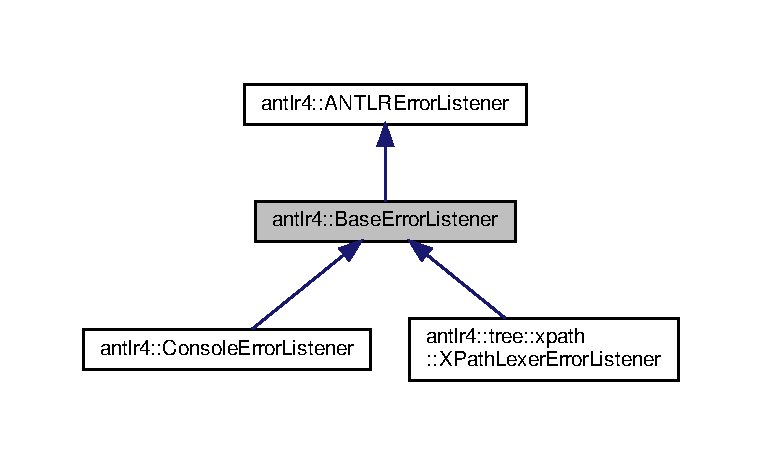
\includegraphics[width=350pt]{classantlr4_1_1BaseErrorListener__inherit__graph}
\end{center}
\end{figure}


Collaboration diagram for antlr4\+:\+:Base\+Error\+Listener\+:
\nopagebreak
\begin{figure}[H]
\begin{center}
\leavevmode
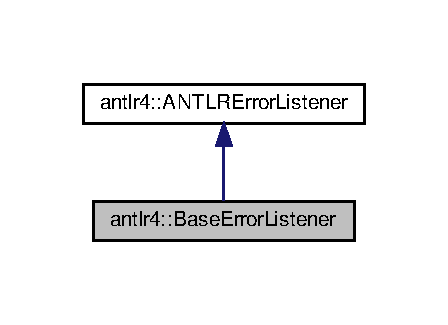
\includegraphics[width=215pt]{classantlr4_1_1BaseErrorListener__coll__graph}
\end{center}
\end{figure}


\subsection{Detailed Description}
Provides an empty default implementation of \hyperlink{classantlr4_1_1ANTLRErrorListener}{A\+N\+T\+L\+R\+Error\+Listener}. The default implementation of each method does nothing, but can be overridden as necessary. 

The documentation for this class was generated from the following files\+:\begin{DoxyCompactItemize}
\item 
Base\+Error\+Listener.\+h\item 
Base\+Error\+Listener.\+cpp\end{DoxyCompactItemize}

\hypertarget{classantlr4_1_1atn_1_1BasicBlockStartState}{}\section{antlr4\+:\+:atn\+:\+:Basic\+Block\+Start\+State Class Reference}
\label{classantlr4_1_1atn_1_1BasicBlockStartState}\index{antlr4\+::atn\+::\+Basic\+Block\+Start\+State@{antlr4\+::atn\+::\+Basic\+Block\+Start\+State}}


Inheritance diagram for antlr4\+:\+:atn\+:\+:Basic\+Block\+Start\+State\+:
\nopagebreak
\begin{figure}[H]
\begin{center}
\leavevmode
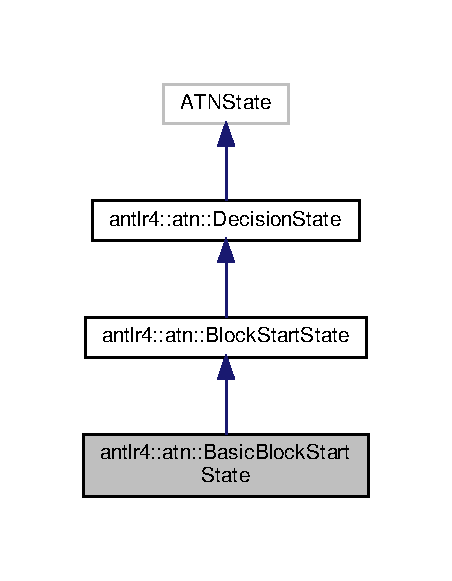
\includegraphics[width=217pt]{classantlr4_1_1atn_1_1BasicBlockStartState__inherit__graph}
\end{center}
\end{figure}


Collaboration diagram for antlr4\+:\+:atn\+:\+:Basic\+Block\+Start\+State\+:
\nopagebreak
\begin{figure}[H]
\begin{center}
\leavevmode
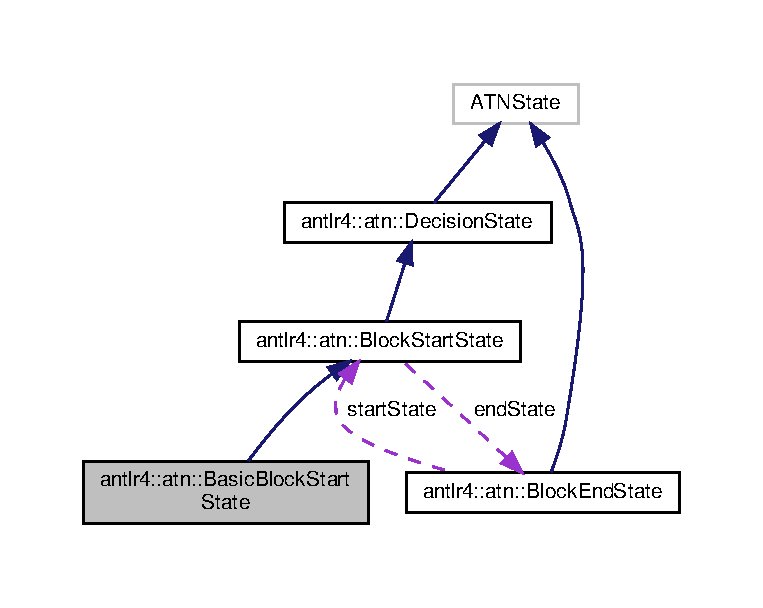
\includegraphics[width=350pt]{classantlr4_1_1atn_1_1BasicBlockStartState__coll__graph}
\end{center}
\end{figure}
\subsection*{Public Member Functions}
\begin{DoxyCompactItemize}
\item 
\mbox{\Hypertarget{classantlr4_1_1atn_1_1BasicBlockStartState_a7cad456274fe68f39e94708f536b72c9}\label{classantlr4_1_1atn_1_1BasicBlockStartState_a7cad456274fe68f39e94708f536b72c9}} 
virtual size\+\_\+t {\bfseries get\+State\+Type} () override
\end{DoxyCompactItemize}
\subsection*{Additional Inherited Members}


The documentation for this class was generated from the following files\+:\begin{DoxyCompactItemize}
\item 
atn/Basic\+Block\+Start\+State.\+h\item 
atn/Basic\+Block\+Start\+State.\+cpp\end{DoxyCompactItemize}

\hypertarget{classantlr4_1_1atn_1_1BasicState}{}\section{antlr4\+:\+:atn\+:\+:Basic\+State Class Reference}
\label{classantlr4_1_1atn_1_1BasicState}\index{antlr4\+::atn\+::\+Basic\+State@{antlr4\+::atn\+::\+Basic\+State}}


Inheritance diagram for antlr4\+:\+:atn\+:\+:Basic\+State\+:
\nopagebreak
\begin{figure}[H]
\begin{center}
\leavevmode
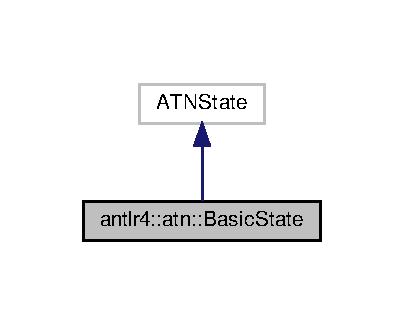
\includegraphics[width=194pt]{classantlr4_1_1atn_1_1BasicState__inherit__graph}
\end{center}
\end{figure}


Collaboration diagram for antlr4\+:\+:atn\+:\+:Basic\+State\+:
\nopagebreak
\begin{figure}[H]
\begin{center}
\leavevmode
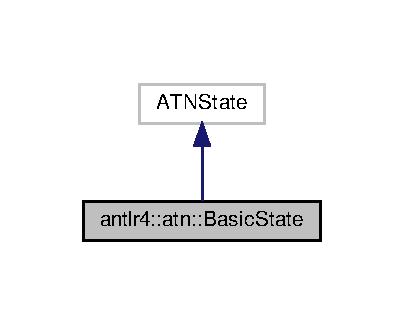
\includegraphics[width=194pt]{classantlr4_1_1atn_1_1BasicState__coll__graph}
\end{center}
\end{figure}
\subsection*{Public Member Functions}
\begin{DoxyCompactItemize}
\item 
\mbox{\Hypertarget{classantlr4_1_1atn_1_1BasicState_a56469de91f944fc01412b906b805313e}\label{classantlr4_1_1atn_1_1BasicState_a56469de91f944fc01412b906b805313e}} 
virtual size\+\_\+t {\bfseries get\+State\+Type} () override
\end{DoxyCompactItemize}


The documentation for this class was generated from the following files\+:\begin{DoxyCompactItemize}
\item 
atn/Basic\+State.\+h\item 
atn/Basic\+State.\+cpp\end{DoxyCompactItemize}

\hypertarget{classantlrcpp_1_1BitSet}{}\section{antlrcpp\+:\+:Bit\+Set Class Reference}
\label{classantlrcpp_1_1BitSet}\index{antlrcpp\+::\+Bit\+Set@{antlrcpp\+::\+Bit\+Set}}


Inheritance diagram for antlrcpp\+:\+:Bit\+Set\+:
\nopagebreak
\begin{figure}[H]
\begin{center}
\leavevmode
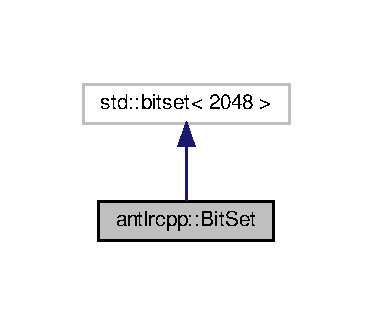
\includegraphics[width=179pt]{classantlrcpp_1_1BitSet__inherit__graph}
\end{center}
\end{figure}


Collaboration diagram for antlrcpp\+:\+:Bit\+Set\+:
\nopagebreak
\begin{figure}[H]
\begin{center}
\leavevmode
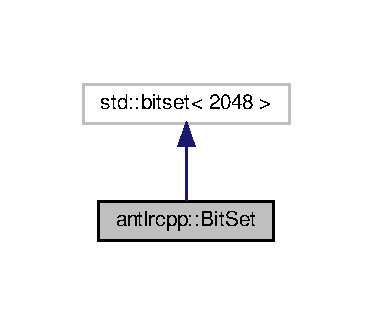
\includegraphics[width=179pt]{classantlrcpp_1_1BitSet__coll__graph}
\end{center}
\end{figure}
\subsection*{Public Member Functions}
\begin{DoxyCompactItemize}
\item 
\mbox{\Hypertarget{classantlrcpp_1_1BitSet_a42f487492a858e90b594a24615241500}\label{classantlrcpp_1_1BitSet_a42f487492a858e90b594a24615241500}} 
size\+\_\+t {\bfseries next\+Set\+Bit} (size\+\_\+t pos) const
\item 
\mbox{\Hypertarget{classantlrcpp_1_1BitSet_a58716f50db7fc6490a2611af9437b6f7}\label{classantlrcpp_1_1BitSet_a58716f50db7fc6490a2611af9437b6f7}} 
std\+::string {\bfseries to\+String} ()
\end{DoxyCompactItemize}
\subsection*{Static Public Member Functions}
\begin{DoxyCompactItemize}
\item 
\mbox{\Hypertarget{classantlrcpp_1_1BitSet_a6c3b0d84d2b16b29a6e1ec3a55b32d6f}\label{classantlrcpp_1_1BitSet_a6c3b0d84d2b16b29a6e1ec3a55b32d6f}} 
static std\+::string {\bfseries sub\+String\+Representation} (const std\+::vector$<$ \hyperlink{classantlrcpp_1_1BitSet}{Bit\+Set} $>$\+::iterator \&begin, const std\+::vector$<$ \hyperlink{classantlrcpp_1_1BitSet}{Bit\+Set} $>$\+::iterator \&end)
\end{DoxyCompactItemize}
\subsection*{Friends}
\begin{DoxyCompactItemize}
\item 
\mbox{\Hypertarget{classantlrcpp_1_1BitSet_aaf73291b783507d962eccd1635aee50f}\label{classantlrcpp_1_1BitSet_aaf73291b783507d962eccd1635aee50f}} 
std\+::wostream \& {\bfseries operator$<$$<$} (std\+::wostream \&os, const \hyperlink{classantlrcpp_1_1BitSet}{Bit\+Set} \&obj)
\end{DoxyCompactItemize}


The documentation for this class was generated from the following file\+:\begin{DoxyCompactItemize}
\item 
support/Bit\+Set.\+h\end{DoxyCompactItemize}

\hypertarget{classantlr4_1_1atn_1_1BlockEndState}{}\section{antlr4\+:\+:atn\+:\+:Block\+End\+State Class Reference}
\label{classantlr4_1_1atn_1_1BlockEndState}\index{antlr4\+::atn\+::\+Block\+End\+State@{antlr4\+::atn\+::\+Block\+End\+State}}


Terminal node of a simple \{.  




{\ttfamily \#include $<$Block\+End\+State.\+h$>$}



Inheritance diagram for antlr4\+:\+:atn\+:\+:Block\+End\+State\+:
\nopagebreak
\begin{figure}[H]
\begin{center}
\leavevmode
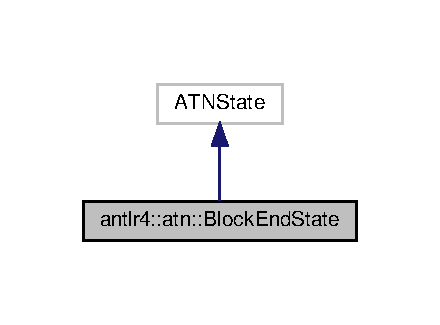
\includegraphics[width=211pt]{classantlr4_1_1atn_1_1BlockEndState__inherit__graph}
\end{center}
\end{figure}


Collaboration diagram for antlr4\+:\+:atn\+:\+:Block\+End\+State\+:
\nopagebreak
\begin{figure}[H]
\begin{center}
\leavevmode
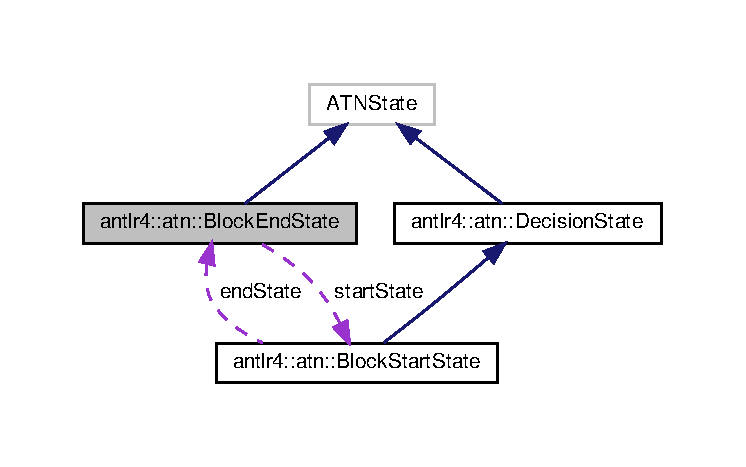
\includegraphics[width=350pt]{classantlr4_1_1atn_1_1BlockEndState__coll__graph}
\end{center}
\end{figure}
\subsection*{Public Member Functions}
\begin{DoxyCompactItemize}
\item 
\mbox{\Hypertarget{classantlr4_1_1atn_1_1BlockEndState_a37596e80fdf84b222c77c51ec343b56e}\label{classantlr4_1_1atn_1_1BlockEndState_a37596e80fdf84b222c77c51ec343b56e}} 
virtual size\+\_\+t {\bfseries get\+State\+Type} () override
\end{DoxyCompactItemize}
\subsection*{Public Attributes}
\begin{DoxyCompactItemize}
\item 
\mbox{\Hypertarget{classantlr4_1_1atn_1_1BlockEndState_a98fb9ca9e750f16d2e961fcd2ef79dee}\label{classantlr4_1_1atn_1_1BlockEndState_a98fb9ca9e750f16d2e961fcd2ef79dee}} 
\hyperlink{classantlr4_1_1atn_1_1BlockStartState}{Block\+Start\+State} $\ast$ {\bfseries start\+State} = nullptr
\end{DoxyCompactItemize}


\subsection{Detailed Description}
Terminal node of a simple \{. 


\begin{DoxyCode}
(a|b|c)\} block. 
\end{DoxyCode}


The documentation for this class was generated from the following files\+:\begin{DoxyCompactItemize}
\item 
atn/Block\+End\+State.\+h\item 
atn/Block\+End\+State.\+cpp\end{DoxyCompactItemize}

\hypertarget{classantlr4_1_1atn_1_1BlockStartState}{}\section{antlr4\+:\+:atn\+:\+:Block\+Start\+State Class Reference}
\label{classantlr4_1_1atn_1_1BlockStartState}\index{antlr4\+::atn\+::\+Block\+Start\+State@{antlr4\+::atn\+::\+Block\+Start\+State}}


The start of a regular \{.  




{\ttfamily \#include $<$Block\+Start\+State.\+h$>$}



Inheritance diagram for antlr4\+:\+:atn\+:\+:Block\+Start\+State\+:
\nopagebreak
\begin{figure}[H]
\begin{center}
\leavevmode
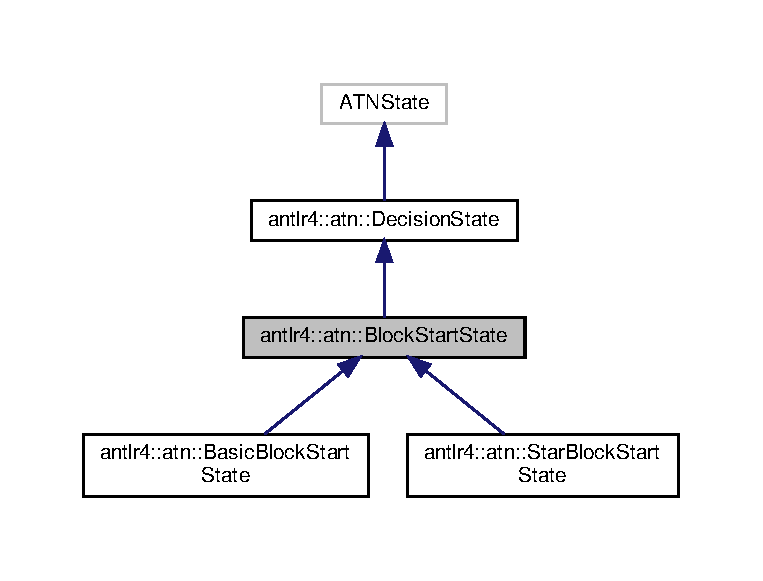
\includegraphics[width=350pt]{classantlr4_1_1atn_1_1BlockStartState__inherit__graph}
\end{center}
\end{figure}


Collaboration diagram for antlr4\+:\+:atn\+:\+:Block\+Start\+State\+:
\nopagebreak
\begin{figure}[H]
\begin{center}
\leavevmode
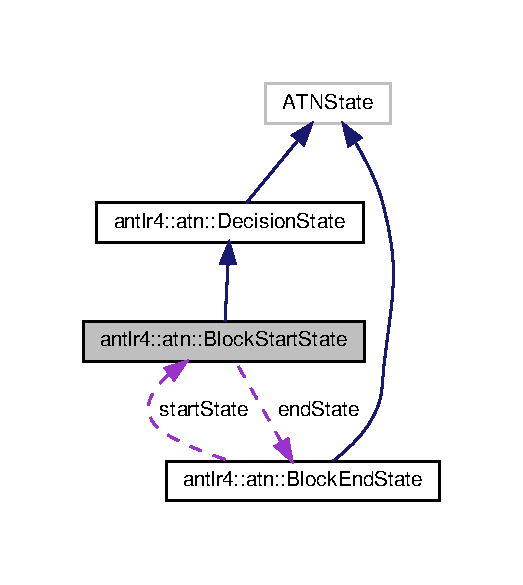
\includegraphics[width=251pt]{classantlr4_1_1atn_1_1BlockStartState__coll__graph}
\end{center}
\end{figure}
\subsection*{Public Attributes}
\begin{DoxyCompactItemize}
\item 
\mbox{\Hypertarget{classantlr4_1_1atn_1_1BlockStartState_aa79f25cca90ec823d50f4a8f7b7ec017}\label{classantlr4_1_1atn_1_1BlockStartState_aa79f25cca90ec823d50f4a8f7b7ec017}} 
\hyperlink{classantlr4_1_1atn_1_1BlockEndState}{Block\+End\+State} $\ast$ {\bfseries end\+State} = nullptr
\end{DoxyCompactItemize}
\subsection*{Additional Inherited Members}


\subsection{Detailed Description}
The start of a regular \{. 


\begin{DoxyCode}
(...)\} block. 
\end{DoxyCode}


The documentation for this class was generated from the following files\+:\begin{DoxyCompactItemize}
\item 
atn/Block\+Start\+State.\+h\item 
atn/Block\+Start\+State.\+cpp\end{DoxyCompactItemize}

\hypertarget{classantlr4_1_1BufferedTokenStream}{}\section{antlr4\+:\+:Buffered\+Token\+Stream Class Reference}
\label{classantlr4_1_1BufferedTokenStream}\index{antlr4\+::\+Buffered\+Token\+Stream@{antlr4\+::\+Buffered\+Token\+Stream}}


{\ttfamily \#include $<$Buffered\+Token\+Stream.\+h$>$}



Inheritance diagram for antlr4\+:\+:Buffered\+Token\+Stream\+:
\nopagebreak
\begin{figure}[H]
\begin{center}
\leavevmode
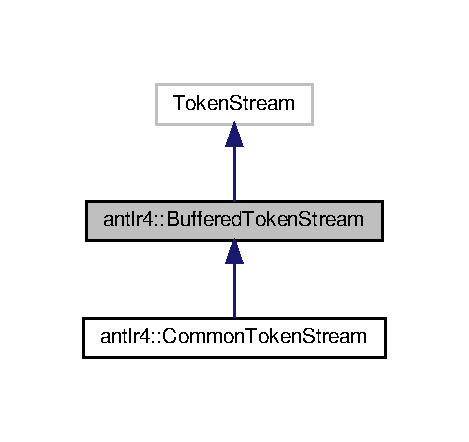
\includegraphics[width=225pt]{classantlr4_1_1BufferedTokenStream__inherit__graph}
\end{center}
\end{figure}


Collaboration diagram for antlr4\+:\+:Buffered\+Token\+Stream\+:
\nopagebreak
\begin{figure}[H]
\begin{center}
\leavevmode
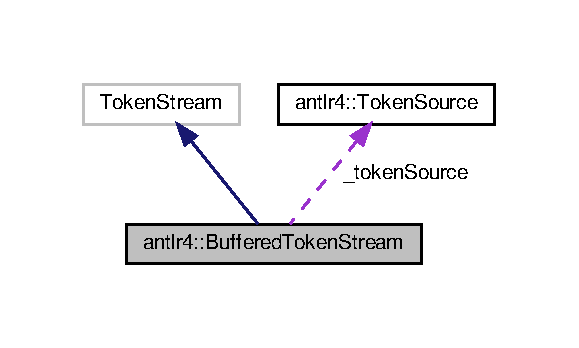
\includegraphics[width=278pt]{classantlr4_1_1BufferedTokenStream__coll__graph}
\end{center}
\end{figure}
\subsection*{Public Member Functions}
\begin{DoxyCompactItemize}
\item 
\mbox{\Hypertarget{classantlr4_1_1BufferedTokenStream_a8745b20dfdbda56d024d3bbd7b1b952b}\label{classantlr4_1_1BufferedTokenStream_a8745b20dfdbda56d024d3bbd7b1b952b}} 
{\bfseries Buffered\+Token\+Stream} (\hyperlink{classantlr4_1_1TokenSource}{Token\+Source} $\ast$token\+Source)
\item 
\mbox{\Hypertarget{classantlr4_1_1BufferedTokenStream_aa80d128b76649cb544a2687392b455ba}\label{classantlr4_1_1BufferedTokenStream_aa80d128b76649cb544a2687392b455ba}} 
{\bfseries Buffered\+Token\+Stream} (const \hyperlink{classantlr4_1_1BufferedTokenStream}{Buffered\+Token\+Stream} \&other)=delete
\item 
\mbox{\Hypertarget{classantlr4_1_1BufferedTokenStream_aa3a4c451709b72c3a1fc3b5e129a0589}\label{classantlr4_1_1BufferedTokenStream_aa3a4c451709b72c3a1fc3b5e129a0589}} 
\hyperlink{classantlr4_1_1BufferedTokenStream}{Buffered\+Token\+Stream} \& {\bfseries operator=} (const \hyperlink{classantlr4_1_1BufferedTokenStream}{Buffered\+Token\+Stream} \&other)=delete
\item 
\mbox{\Hypertarget{classantlr4_1_1BufferedTokenStream_adfb641a7c1014a32c25a8de2161d980b}\label{classantlr4_1_1BufferedTokenStream_adfb641a7c1014a32c25a8de2161d980b}} 
virtual \hyperlink{classantlr4_1_1TokenSource}{Token\+Source} $\ast$ {\bfseries get\+Token\+Source} () const override
\item 
\mbox{\Hypertarget{classantlr4_1_1BufferedTokenStream_a3df0d36a9f48af46e957287d6f5242a5}\label{classantlr4_1_1BufferedTokenStream_a3df0d36a9f48af46e957287d6f5242a5}} 
virtual size\+\_\+t {\bfseries index} () override
\item 
\mbox{\Hypertarget{classantlr4_1_1BufferedTokenStream_a04ae6c5de3677e6836f162655c710a22}\label{classantlr4_1_1BufferedTokenStream_a04ae6c5de3677e6836f162655c710a22}} 
virtual ssize\+\_\+t {\bfseries mark} () override
\item 
\mbox{\Hypertarget{classantlr4_1_1BufferedTokenStream_af881ee9a58087055bc33c4d8ca2f64e7}\label{classantlr4_1_1BufferedTokenStream_af881ee9a58087055bc33c4d8ca2f64e7}} 
virtual void {\bfseries release} (ssize\+\_\+t marker) override
\item 
\mbox{\Hypertarget{classantlr4_1_1BufferedTokenStream_a258dec8c7d9d2cf5ee0b69105cfab9e4}\label{classantlr4_1_1BufferedTokenStream_a258dec8c7d9d2cf5ee0b69105cfab9e4}} 
virtual void {\bfseries reset} ()
\item 
\mbox{\Hypertarget{classantlr4_1_1BufferedTokenStream_a96d113899cac110b51147147d9cb7b7a}\label{classantlr4_1_1BufferedTokenStream_a96d113899cac110b51147147d9cb7b7a}} 
virtual void {\bfseries seek} (size\+\_\+t index) override
\item 
\mbox{\Hypertarget{classantlr4_1_1BufferedTokenStream_abacc9f5776ad27c0dde09daea4930952}\label{classantlr4_1_1BufferedTokenStream_abacc9f5776ad27c0dde09daea4930952}} 
virtual size\+\_\+t {\bfseries size} () override
\item 
\mbox{\Hypertarget{classantlr4_1_1BufferedTokenStream_a23f513618817ff1a02f4bd5f8bad57c7}\label{classantlr4_1_1BufferedTokenStream_a23f513618817ff1a02f4bd5f8bad57c7}} 
virtual void {\bfseries consume} () override
\item 
\mbox{\Hypertarget{classantlr4_1_1BufferedTokenStream_a409b9b2413d354d3e675f0e19ca80179}\label{classantlr4_1_1BufferedTokenStream_a409b9b2413d354d3e675f0e19ca80179}} 
virtual \hyperlink{classantlr4_1_1Token}{Token} $\ast$ {\bfseries get} (size\+\_\+t i) const override
\item 
\mbox{\Hypertarget{classantlr4_1_1BufferedTokenStream_a9afaa76373aa65443db2f7d8c60a723c}\label{classantlr4_1_1BufferedTokenStream_a9afaa76373aa65443db2f7d8c60a723c}} 
virtual std\+::vector$<$ \hyperlink{classantlr4_1_1Token}{Token} $\ast$ $>$ \hyperlink{classantlr4_1_1BufferedTokenStream_a9afaa76373aa65443db2f7d8c60a723c}{get} (size\+\_\+t start, size\+\_\+t stop)
\begin{DoxyCompactList}\small\item\em Get all tokens from start..stop inclusively. \end{DoxyCompactList}\item 
\mbox{\Hypertarget{classantlr4_1_1BufferedTokenStream_ac13d29ad96e08c0da1f0474faa035520}\label{classantlr4_1_1BufferedTokenStream_ac13d29ad96e08c0da1f0474faa035520}} 
virtual size\+\_\+t {\bfseries LA} (ssize\+\_\+t i) override
\item 
\mbox{\Hypertarget{classantlr4_1_1BufferedTokenStream_a6f373d718e438523a5779941b96d7c01}\label{classantlr4_1_1BufferedTokenStream_a6f373d718e438523a5779941b96d7c01}} 
virtual \hyperlink{classantlr4_1_1Token}{Token} $\ast$ {\bfseries LT} (ssize\+\_\+t k) override
\item 
\mbox{\Hypertarget{classantlr4_1_1BufferedTokenStream_a3286f252ebc773cd6f4c1bd375e1012a}\label{classantlr4_1_1BufferedTokenStream_a3286f252ebc773cd6f4c1bd375e1012a}} 
virtual void \hyperlink{classantlr4_1_1BufferedTokenStream_a3286f252ebc773cd6f4c1bd375e1012a}{set\+Token\+Source} (\hyperlink{classantlr4_1_1TokenSource}{Token\+Source} $\ast$token\+Source)
\begin{DoxyCompactList}\small\item\em Reset this token stream by setting its token source. \end{DoxyCompactList}\item 
\mbox{\Hypertarget{classantlr4_1_1BufferedTokenStream_af6bfd7d726c911f192bae1eb6aeb571c}\label{classantlr4_1_1BufferedTokenStream_af6bfd7d726c911f192bae1eb6aeb571c}} 
virtual std\+::vector$<$ \hyperlink{classantlr4_1_1Token}{Token} $\ast$ $>$ {\bfseries get\+Tokens} ()
\item 
\mbox{\Hypertarget{classantlr4_1_1BufferedTokenStream_a1a2de27fefe90b711a500be49857c2da}\label{classantlr4_1_1BufferedTokenStream_a1a2de27fefe90b711a500be49857c2da}} 
virtual std\+::vector$<$ \hyperlink{classantlr4_1_1Token}{Token} $\ast$ $>$ {\bfseries get\+Tokens} (size\+\_\+t start, size\+\_\+t stop)
\item 
virtual std\+::vector$<$ \hyperlink{classantlr4_1_1Token}{Token} $\ast$ $>$ \hyperlink{classantlr4_1_1BufferedTokenStream_a1da75f1766b2758b16be452bc1e06681}{get\+Tokens} (size\+\_\+t start, size\+\_\+t stop, const std\+::vector$<$ size\+\_\+t $>$ \&types)
\begin{DoxyCompactList}\small\item\em Given a start and stop index, return a List of all tokens in the token type Bit\+Set. Return null if no tokens were found. This method looks at both on and off channel tokens. \end{DoxyCompactList}\item 
\mbox{\Hypertarget{classantlr4_1_1BufferedTokenStream_a18ddeab3509ccc606731b07a0c81725e}\label{classantlr4_1_1BufferedTokenStream_a18ddeab3509ccc606731b07a0c81725e}} 
virtual std\+::vector$<$ \hyperlink{classantlr4_1_1Token}{Token} $\ast$ $>$ {\bfseries get\+Tokens} (size\+\_\+t start, size\+\_\+t stop, size\+\_\+t ttype)
\item 
virtual std\+::vector$<$ \hyperlink{classantlr4_1_1Token}{Token} $\ast$ $>$ \hyperlink{classantlr4_1_1BufferedTokenStream_a6c260c6968178e322e5651ef0766925e}{get\+Hidden\+Tokens\+To\+Right} (size\+\_\+t token\+Index, ssize\+\_\+t channel)
\item 
virtual std\+::vector$<$ \hyperlink{classantlr4_1_1Token}{Token} $\ast$ $>$ \hyperlink{classantlr4_1_1BufferedTokenStream_a962f9c5cfb338e728948510a687174ec}{get\+Hidden\+Tokens\+To\+Right} (size\+\_\+t token\+Index)
\begin{DoxyCompactList}\small\item\em Collect all hidden tokens (any off-\/default channel) to the right of the current token up until we see a token on D\+E\+F\+A\+U\+L\+T\+\_\+\+T\+O\+K\+E\+N\+\_\+\+C\+H\+A\+N\+N\+EL or E\+OF. \end{DoxyCompactList}\item 
virtual std\+::vector$<$ \hyperlink{classantlr4_1_1Token}{Token} $\ast$ $>$ \hyperlink{classantlr4_1_1BufferedTokenStream_ac43a075d6f0ecbda219eef4a9e4633ee}{get\+Hidden\+Tokens\+To\+Left} (size\+\_\+t token\+Index, ssize\+\_\+t channel)
\begin{DoxyCompactList}\small\item\em Collect all tokens on specified channel to the left of the current token up until we see a token on D\+E\+F\+A\+U\+L\+T\+\_\+\+T\+O\+K\+E\+N\+\_\+\+C\+H\+A\+N\+N\+EL. If channel is -\/1, find any non default channel token. \end{DoxyCompactList}\item 
virtual std\+::vector$<$ \hyperlink{classantlr4_1_1Token}{Token} $\ast$ $>$ \hyperlink{classantlr4_1_1BufferedTokenStream_aa6f2ca68abd8075329bba1da12970493}{get\+Hidden\+Tokens\+To\+Left} (size\+\_\+t token\+Index)
\begin{DoxyCompactList}\small\item\em Collect all hidden tokens (any off-\/default channel) to the left of the current token up until we see a token on D\+E\+F\+A\+U\+L\+T\+\_\+\+T\+O\+K\+E\+N\+\_\+\+C\+H\+A\+N\+N\+EL. \end{DoxyCompactList}\item 
virtual std\+::string \hyperlink{classantlr4_1_1BufferedTokenStream_ac623cc25ef85bed24d4a387bc6ad5663}{get\+Source\+Name} () const override
\item 
\mbox{\Hypertarget{classantlr4_1_1BufferedTokenStream_ad7a1573fe9be79daf42c793ebfe1abc6}\label{classantlr4_1_1BufferedTokenStream_ad7a1573fe9be79daf42c793ebfe1abc6}} 
virtual std\+::string {\bfseries get\+Text} () override
\item 
\mbox{\Hypertarget{classantlr4_1_1BufferedTokenStream_a330ddd9c7472b2fa9c59eb24ec1f4b94}\label{classantlr4_1_1BufferedTokenStream_a330ddd9c7472b2fa9c59eb24ec1f4b94}} 
virtual std\+::string {\bfseries get\+Text} (const \hyperlink{classantlr4_1_1misc_1_1Interval}{misc\+::\+Interval} \&interval) override
\item 
\mbox{\Hypertarget{classantlr4_1_1BufferedTokenStream_a9daa8586537ac66a8ad4152e26865199}\label{classantlr4_1_1BufferedTokenStream_a9daa8586537ac66a8ad4152e26865199}} 
virtual std\+::string {\bfseries get\+Text} (\hyperlink{classantlr4_1_1RuleContext}{Rule\+Context} $\ast$ctx) override
\item 
\mbox{\Hypertarget{classantlr4_1_1BufferedTokenStream_a2090d846bb61a625a8ca23483571cebd}\label{classantlr4_1_1BufferedTokenStream_a2090d846bb61a625a8ca23483571cebd}} 
virtual std\+::string {\bfseries get\+Text} (\hyperlink{classantlr4_1_1Token}{Token} $\ast$start, \hyperlink{classantlr4_1_1Token}{Token} $\ast$stop) override
\item 
\mbox{\Hypertarget{classantlr4_1_1BufferedTokenStream_a373c27c4d4ec7358ba6985f4839e988a}\label{classantlr4_1_1BufferedTokenStream_a373c27c4d4ec7358ba6985f4839e988a}} 
virtual void \hyperlink{classantlr4_1_1BufferedTokenStream_a373c27c4d4ec7358ba6985f4839e988a}{fill} ()
\begin{DoxyCompactList}\small\item\em Get all tokens from lexer until E\+OF. \end{DoxyCompactList}\end{DoxyCompactItemize}
\subsection*{Protected Attributes}
\begin{DoxyCompactItemize}
\item 
\hyperlink{classantlr4_1_1TokenSource}{Token\+Source} $\ast$ \hyperlink{classantlr4_1_1BufferedTokenStream_aa0a28e43e9e3329ddfe404804f726023}{\+\_\+token\+Source}
\item 
std\+::vector$<$ std\+::unique\+\_\+ptr$<$ \hyperlink{classantlr4_1_1Token}{Token} $>$ $>$ \hyperlink{classantlr4_1_1BufferedTokenStream_ac681a8540466ec9aab6cff49bbcbdb4b}{\+\_\+tokens}
\item 
size\+\_\+t \hyperlink{classantlr4_1_1BufferedTokenStream_aa8ab272f9ef3f5195ef8aeb4da15f9ca}{\+\_\+p}
\item 
bool \hyperlink{classantlr4_1_1BufferedTokenStream_a400797b54a3d7d151aa0ace27e766e8e}{\+\_\+fetched\+E\+OF}
\end{DoxyCompactItemize}


\subsection{Detailed Description}
This implementation of \hyperlink{}{Token\+Stream} loads tokens from a \hyperlink{classantlr4_1_1TokenSource}{Token\+Source} on-\/demand, and places the tokens in a buffer to provide access to any previous token by index.

This token stream ignores the value of \hyperlink{classantlr4_1_1Token_a92991c0566e4cb00ae2c5f9e7d8fe6b4}{Token\#get\+Channel}. If your parser requires the token stream filter tokens to only those on a particular channel, such as \hyperlink{classantlr4_1_1Token_a699cbc56affbddc079561e175cba8435}{Token\#\+D\+E\+F\+A\+U\+L\+T\+\_\+\+C\+H\+A\+N\+N\+EL} or \hyperlink{classantlr4_1_1Token_af9bee187eba93f908d76d6406883424a}{Token\#\+H\+I\+D\+D\+E\+N\+\_\+\+C\+H\+A\+N\+N\+EL}, use a filtering token stream such a \hyperlink{classantlr4_1_1CommonTokenStream}{Common\+Token\+Stream}.

\subsection{Member Function Documentation}
\mbox{\Hypertarget{classantlr4_1_1BufferedTokenStream_ac43a075d6f0ecbda219eef4a9e4633ee}\label{classantlr4_1_1BufferedTokenStream_ac43a075d6f0ecbda219eef4a9e4633ee}} 
\index{antlr4\+::\+Buffered\+Token\+Stream@{antlr4\+::\+Buffered\+Token\+Stream}!get\+Hidden\+Tokens\+To\+Left@{get\+Hidden\+Tokens\+To\+Left}}
\index{get\+Hidden\+Tokens\+To\+Left@{get\+Hidden\+Tokens\+To\+Left}!antlr4\+::\+Buffered\+Token\+Stream@{antlr4\+::\+Buffered\+Token\+Stream}}
\subsubsection{\texorpdfstring{get\+Hidden\+Tokens\+To\+Left()}{getHiddenTokensToLeft()}\hspace{0.1cm}{\footnotesize\ttfamily [1/2]}}
{\footnotesize\ttfamily std\+::vector$<$ \hyperlink{classantlr4_1_1Token}{Token} $\ast$ $>$ Buffered\+Token\+Stream\+::get\+Hidden\+Tokens\+To\+Left (\begin{DoxyParamCaption}\item[{size\+\_\+t}]{token\+Index,  }\item[{ssize\+\_\+t}]{channel }\end{DoxyParamCaption})\hspace{0.3cm}{\ttfamily [virtual]}}



Collect all tokens on specified channel to the left of the current token up until we see a token on D\+E\+F\+A\+U\+L\+T\+\_\+\+T\+O\+K\+E\+N\+\_\+\+C\+H\+A\+N\+N\+EL. If channel is -\/1, find any non default channel token. 

\mbox{\Hypertarget{classantlr4_1_1BufferedTokenStream_aa6f2ca68abd8075329bba1da12970493}\label{classantlr4_1_1BufferedTokenStream_aa6f2ca68abd8075329bba1da12970493}} 
\index{antlr4\+::\+Buffered\+Token\+Stream@{antlr4\+::\+Buffered\+Token\+Stream}!get\+Hidden\+Tokens\+To\+Left@{get\+Hidden\+Tokens\+To\+Left}}
\index{get\+Hidden\+Tokens\+To\+Left@{get\+Hidden\+Tokens\+To\+Left}!antlr4\+::\+Buffered\+Token\+Stream@{antlr4\+::\+Buffered\+Token\+Stream}}
\subsubsection{\texorpdfstring{get\+Hidden\+Tokens\+To\+Left()}{getHiddenTokensToLeft()}\hspace{0.1cm}{\footnotesize\ttfamily [2/2]}}
{\footnotesize\ttfamily std\+::vector$<$ \hyperlink{classantlr4_1_1Token}{Token} $\ast$ $>$ Buffered\+Token\+Stream\+::get\+Hidden\+Tokens\+To\+Left (\begin{DoxyParamCaption}\item[{size\+\_\+t}]{token\+Index }\end{DoxyParamCaption})\hspace{0.3cm}{\ttfamily [virtual]}}



Collect all hidden tokens (any off-\/default channel) to the left of the current token up until we see a token on D\+E\+F\+A\+U\+L\+T\+\_\+\+T\+O\+K\+E\+N\+\_\+\+C\+H\+A\+N\+N\+EL. 

\mbox{\Hypertarget{classantlr4_1_1BufferedTokenStream_a6c260c6968178e322e5651ef0766925e}\label{classantlr4_1_1BufferedTokenStream_a6c260c6968178e322e5651ef0766925e}} 
\index{antlr4\+::\+Buffered\+Token\+Stream@{antlr4\+::\+Buffered\+Token\+Stream}!get\+Hidden\+Tokens\+To\+Right@{get\+Hidden\+Tokens\+To\+Right}}
\index{get\+Hidden\+Tokens\+To\+Right@{get\+Hidden\+Tokens\+To\+Right}!antlr4\+::\+Buffered\+Token\+Stream@{antlr4\+::\+Buffered\+Token\+Stream}}
\subsubsection{\texorpdfstring{get\+Hidden\+Tokens\+To\+Right()}{getHiddenTokensToRight()}\hspace{0.1cm}{\footnotesize\ttfamily [1/2]}}
{\footnotesize\ttfamily std\+::vector$<$ \hyperlink{classantlr4_1_1Token}{Token} $\ast$ $>$ Buffered\+Token\+Stream\+::get\+Hidden\+Tokens\+To\+Right (\begin{DoxyParamCaption}\item[{size\+\_\+t}]{token\+Index,  }\item[{ssize\+\_\+t}]{channel }\end{DoxyParamCaption})\hspace{0.3cm}{\ttfamily [virtual]}}

Collect all tokens on specified channel to the right of the current token up until we see a token on D\+E\+F\+A\+U\+L\+T\+\_\+\+T\+O\+K\+E\+N\+\_\+\+C\+H\+A\+N\+N\+EL or E\+OF. If channel is -\/1, find any non default channel token. \mbox{\Hypertarget{classantlr4_1_1BufferedTokenStream_a962f9c5cfb338e728948510a687174ec}\label{classantlr4_1_1BufferedTokenStream_a962f9c5cfb338e728948510a687174ec}} 
\index{antlr4\+::\+Buffered\+Token\+Stream@{antlr4\+::\+Buffered\+Token\+Stream}!get\+Hidden\+Tokens\+To\+Right@{get\+Hidden\+Tokens\+To\+Right}}
\index{get\+Hidden\+Tokens\+To\+Right@{get\+Hidden\+Tokens\+To\+Right}!antlr4\+::\+Buffered\+Token\+Stream@{antlr4\+::\+Buffered\+Token\+Stream}}
\subsubsection{\texorpdfstring{get\+Hidden\+Tokens\+To\+Right()}{getHiddenTokensToRight()}\hspace{0.1cm}{\footnotesize\ttfamily [2/2]}}
{\footnotesize\ttfamily std\+::vector$<$ \hyperlink{classantlr4_1_1Token}{Token} $\ast$ $>$ Buffered\+Token\+Stream\+::get\+Hidden\+Tokens\+To\+Right (\begin{DoxyParamCaption}\item[{size\+\_\+t}]{token\+Index }\end{DoxyParamCaption})\hspace{0.3cm}{\ttfamily [virtual]}}



Collect all hidden tokens (any off-\/default channel) to the right of the current token up until we see a token on D\+E\+F\+A\+U\+L\+T\+\_\+\+T\+O\+K\+E\+N\+\_\+\+C\+H\+A\+N\+N\+EL or E\+OF. 

\mbox{\Hypertarget{classantlr4_1_1BufferedTokenStream_ac623cc25ef85bed24d4a387bc6ad5663}\label{classantlr4_1_1BufferedTokenStream_ac623cc25ef85bed24d4a387bc6ad5663}} 
\index{antlr4\+::\+Buffered\+Token\+Stream@{antlr4\+::\+Buffered\+Token\+Stream}!get\+Source\+Name@{get\+Source\+Name}}
\index{get\+Source\+Name@{get\+Source\+Name}!antlr4\+::\+Buffered\+Token\+Stream@{antlr4\+::\+Buffered\+Token\+Stream}}
\subsubsection{\texorpdfstring{get\+Source\+Name()}{getSourceName()}}
{\footnotesize\ttfamily std\+::string Buffered\+Token\+Stream\+::get\+Source\+Name (\begin{DoxyParamCaption}{ }\end{DoxyParamCaption}) const\hspace{0.3cm}{\ttfamily [override]}, {\ttfamily [virtual]}}

Get the text of all tokens in this buffer. \mbox{\Hypertarget{classantlr4_1_1BufferedTokenStream_a1da75f1766b2758b16be452bc1e06681}\label{classantlr4_1_1BufferedTokenStream_a1da75f1766b2758b16be452bc1e06681}} 
\index{antlr4\+::\+Buffered\+Token\+Stream@{antlr4\+::\+Buffered\+Token\+Stream}!get\+Tokens@{get\+Tokens}}
\index{get\+Tokens@{get\+Tokens}!antlr4\+::\+Buffered\+Token\+Stream@{antlr4\+::\+Buffered\+Token\+Stream}}
\subsubsection{\texorpdfstring{get\+Tokens()}{getTokens()}}
{\footnotesize\ttfamily std\+::vector$<$ \hyperlink{classantlr4_1_1Token}{Token} $\ast$ $>$ Buffered\+Token\+Stream\+::get\+Tokens (\begin{DoxyParamCaption}\item[{size\+\_\+t}]{start,  }\item[{size\+\_\+t}]{stop,  }\item[{const std\+::vector$<$ size\+\_\+t $>$ \&}]{types }\end{DoxyParamCaption})\hspace{0.3cm}{\ttfamily [virtual]}}



Given a start and stop index, return a List of all tokens in the token type Bit\+Set. Return null if no tokens were found. This method looks at both on and off channel tokens. 



\subsection{Member Data Documentation}
\mbox{\Hypertarget{classantlr4_1_1BufferedTokenStream_a400797b54a3d7d151aa0ace27e766e8e}\label{classantlr4_1_1BufferedTokenStream_a400797b54a3d7d151aa0ace27e766e8e}} 
\index{antlr4\+::\+Buffered\+Token\+Stream@{antlr4\+::\+Buffered\+Token\+Stream}!\+\_\+fetched\+E\+OF@{\+\_\+fetched\+E\+OF}}
\index{\+\_\+fetched\+E\+OF@{\+\_\+fetched\+E\+OF}!antlr4\+::\+Buffered\+Token\+Stream@{antlr4\+::\+Buffered\+Token\+Stream}}
\subsubsection{\texorpdfstring{\+\_\+fetched\+E\+OF}{\_fetchedEOF}}
{\footnotesize\ttfamily bool antlr4\+::\+Buffered\+Token\+Stream\+::\+\_\+fetched\+E\+OF\hspace{0.3cm}{\ttfamily [protected]}}

Indicates whether the \hyperlink{}{Token\#\+E\+OF} token has been fetched from \hyperlink{}{token\+Source} and added to \hyperlink{}{tokens}. This field improves performance for the following cases\+:


\begin{DoxyItemize}
\item \hyperlink{}{consume}\+: The lookahead check in \hyperlink{}{consume} to prevent consuming the E\+OF symbol is optimized by checking the values of \hyperlink{}{fetched\+E\+OF} and \hyperlink{}{p} instead of calling \hyperlink{}{LA}. 
\item \hyperlink{}{fetch}\+: The check to prevent adding multiple E\+OF symbols into \hyperlink{}{tokens} is trivial with this field. 
\begin{DoxyItemize}
\item 
\end{DoxyItemize}
\end{DoxyItemize}\mbox{\Hypertarget{classantlr4_1_1BufferedTokenStream_aa8ab272f9ef3f5195ef8aeb4da15f9ca}\label{classantlr4_1_1BufferedTokenStream_aa8ab272f9ef3f5195ef8aeb4da15f9ca}} 
\index{antlr4\+::\+Buffered\+Token\+Stream@{antlr4\+::\+Buffered\+Token\+Stream}!\+\_\+p@{\+\_\+p}}
\index{\+\_\+p@{\+\_\+p}!antlr4\+::\+Buffered\+Token\+Stream@{antlr4\+::\+Buffered\+Token\+Stream}}
\subsubsection{\texorpdfstring{\+\_\+p}{\_p}}
{\footnotesize\ttfamily size\+\_\+t antlr4\+::\+Buffered\+Token\+Stream\+::\+\_\+p\hspace{0.3cm}{\ttfamily [protected]}}

The index into \hyperlink{}{tokens} of the current token (next token to \hyperlink{}{consume}). \hyperlink{}{tokens}
\begin{DoxyCode}
[ 
\end{DoxyCode}
 \hyperlink{}{p}
\begin{DoxyCode}
] 
\end{DoxyCode}
 should be \hyperlink{}{L\+T(1)}.

This field is set to -\/1 when the stream is first constructed or when \hyperlink{classantlr4_1_1BufferedTokenStream_a3286f252ebc773cd6f4c1bd375e1012a}{set\+Token\+Source} is called, indicating that the first token has not yet been fetched from the token source. For additional information, see the documentation of \hyperlink{}{Int\+Stream} for a description of Initializing Methods.\mbox{\Hypertarget{classantlr4_1_1BufferedTokenStream_ac681a8540466ec9aab6cff49bbcbdb4b}\label{classantlr4_1_1BufferedTokenStream_ac681a8540466ec9aab6cff49bbcbdb4b}} 
\index{antlr4\+::\+Buffered\+Token\+Stream@{antlr4\+::\+Buffered\+Token\+Stream}!\+\_\+tokens@{\+\_\+tokens}}
\index{\+\_\+tokens@{\+\_\+tokens}!antlr4\+::\+Buffered\+Token\+Stream@{antlr4\+::\+Buffered\+Token\+Stream}}
\subsubsection{\texorpdfstring{\+\_\+tokens}{\_tokens}}
{\footnotesize\ttfamily std\+::vector$<$std\+::unique\+\_\+ptr$<$\hyperlink{classantlr4_1_1Token}{Token}$>$ $>$ antlr4\+::\+Buffered\+Token\+Stream\+::\+\_\+tokens\hspace{0.3cm}{\ttfamily [protected]}}

A collection of all tokens fetched from the token source. The list is considered a complete view of the input once \hyperlink{}{fetched\+E\+OF} is set to
\begin{DoxyCode}
\textcolor{keyword}{true} 
\end{DoxyCode}
 . \mbox{\Hypertarget{classantlr4_1_1BufferedTokenStream_aa0a28e43e9e3329ddfe404804f726023}\label{classantlr4_1_1BufferedTokenStream_aa0a28e43e9e3329ddfe404804f726023}} 
\index{antlr4\+::\+Buffered\+Token\+Stream@{antlr4\+::\+Buffered\+Token\+Stream}!\+\_\+token\+Source@{\+\_\+token\+Source}}
\index{\+\_\+token\+Source@{\+\_\+token\+Source}!antlr4\+::\+Buffered\+Token\+Stream@{antlr4\+::\+Buffered\+Token\+Stream}}
\subsubsection{\texorpdfstring{\+\_\+token\+Source}{\_tokenSource}}
{\footnotesize\ttfamily \hyperlink{classantlr4_1_1TokenSource}{Token\+Source}$\ast$ antlr4\+::\+Buffered\+Token\+Stream\+::\+\_\+token\+Source\hspace{0.3cm}{\ttfamily [protected]}}

The \hyperlink{classantlr4_1_1TokenSource}{Token\+Source} from which tokens for this stream are fetched. 

The documentation for this class was generated from the following files\+:\begin{DoxyCompactItemize}
\item 
Buffered\+Token\+Stream.\+h\item 
Buffered\+Token\+Stream.\+cpp\end{DoxyCompactItemize}

\hypertarget{classantlr4_1_1CancellationException}{}\section{antlr4\+:\+:Cancellation\+Exception Class Reference}
\label{classantlr4_1_1CancellationException}\index{antlr4\+::\+Cancellation\+Exception@{antlr4\+::\+Cancellation\+Exception}}


Inheritance diagram for antlr4\+:\+:Cancellation\+Exception\+:
\nopagebreak
\begin{figure}[H]
\begin{center}
\leavevmode
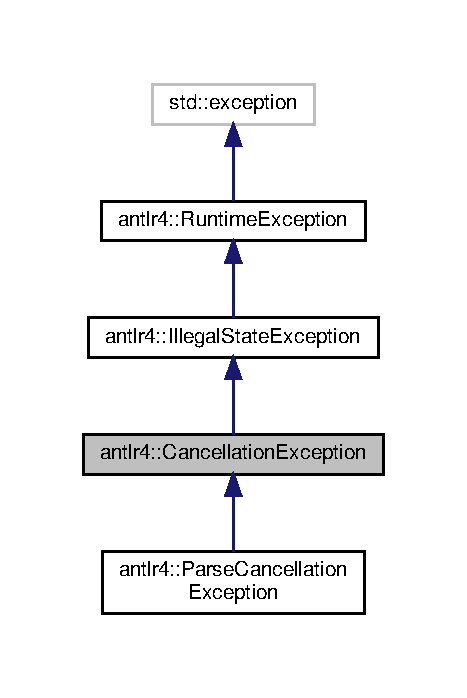
\includegraphics[width=224pt]{classantlr4_1_1CancellationException__inherit__graph}
\end{center}
\end{figure}


Collaboration diagram for antlr4\+:\+:Cancellation\+Exception\+:
\nopagebreak
\begin{figure}[H]
\begin{center}
\leavevmode
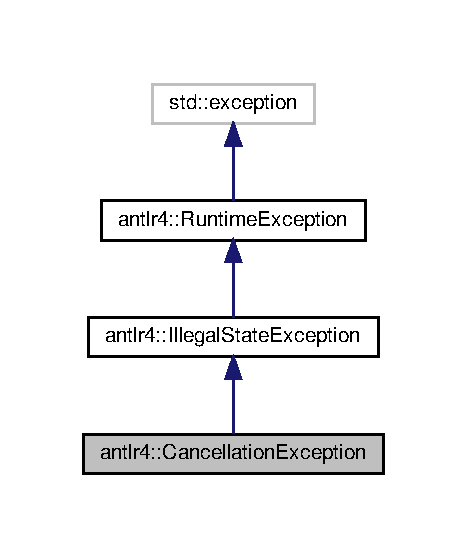
\includegraphics[width=224pt]{classantlr4_1_1CancellationException__coll__graph}
\end{center}
\end{figure}
\subsection*{Public Member Functions}
\begin{DoxyCompactItemize}
\item 
\mbox{\Hypertarget{classantlr4_1_1CancellationException_ad8d9c4154d9f3f68fcb5ac40516ee574}\label{classantlr4_1_1CancellationException_ad8d9c4154d9f3f68fcb5ac40516ee574}} 
{\bfseries Cancellation\+Exception} (const std\+::string \&msg=\char`\"{}\char`\"{})
\item 
\mbox{\Hypertarget{classantlr4_1_1CancellationException_aca7427f541200bf2a5555254e24f2ede}\label{classantlr4_1_1CancellationException_aca7427f541200bf2a5555254e24f2ede}} 
{\bfseries Cancellation\+Exception} (\hyperlink{classantlr4_1_1CancellationException}{Cancellation\+Exception} const \&)=default
\item 
\mbox{\Hypertarget{classantlr4_1_1CancellationException_a7f2671b44cc18b718e37b23ed9c8640b}\label{classantlr4_1_1CancellationException_a7f2671b44cc18b718e37b23ed9c8640b}} 
\hyperlink{classantlr4_1_1CancellationException}{Cancellation\+Exception} \& {\bfseries operator=} (\hyperlink{classantlr4_1_1CancellationException}{Cancellation\+Exception} const \&)=default
\end{DoxyCompactItemize}


The documentation for this class was generated from the following files\+:\begin{DoxyCompactItemize}
\item 
Exceptions.\+h\item 
Exceptions.\+cpp\end{DoxyCompactItemize}

\hypertarget{classantlr4_1_1CommonToken}{}\section{antlr4\+:\+:Common\+Token Class Reference}
\label{classantlr4_1_1CommonToken}\index{antlr4\+::\+Common\+Token@{antlr4\+::\+Common\+Token}}


Inheritance diagram for antlr4\+:\+:Common\+Token\+:
\nopagebreak
\begin{figure}[H]
\begin{center}
\leavevmode
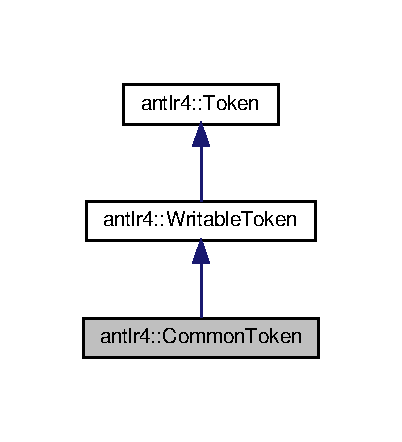
\includegraphics[width=193pt]{classantlr4_1_1CommonToken__inherit__graph}
\end{center}
\end{figure}


Collaboration diagram for antlr4\+:\+:Common\+Token\+:
\nopagebreak
\begin{figure}[H]
\begin{center}
\leavevmode
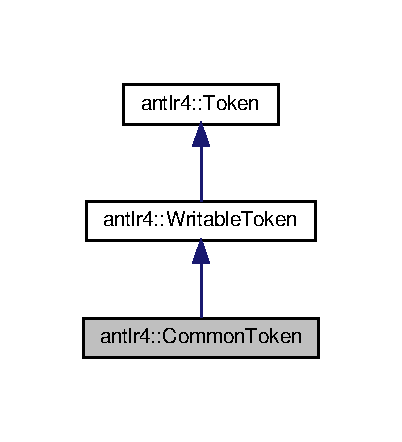
\includegraphics[width=193pt]{classantlr4_1_1CommonToken__coll__graph}
\end{center}
\end{figure}
\subsection*{Public Member Functions}
\begin{DoxyCompactItemize}
\item 
\hyperlink{classantlr4_1_1CommonToken_ae611986affd43e33d45ec933b602e3d6}{Common\+Token} (size\+\_\+t type)
\item 
\mbox{\Hypertarget{classantlr4_1_1CommonToken_a87885416f03f8aa19a5ea1ad1c6d9924}\label{classantlr4_1_1CommonToken_a87885416f03f8aa19a5ea1ad1c6d9924}} 
{\bfseries Common\+Token} (std\+::pair$<$ \hyperlink{classantlr4_1_1TokenSource}{Token\+Source} $\ast$, Char\+Stream $\ast$$>$ source, size\+\_\+t type, size\+\_\+t channel, size\+\_\+t start, size\+\_\+t stop)
\item 
\hyperlink{classantlr4_1_1CommonToken_a7da9b35d9ae9484244b5567e3bce7cb4}{Common\+Token} (size\+\_\+t type, const std\+::string \&text)
\item 
\hyperlink{classantlr4_1_1CommonToken_a7e8aa41e9bf31b4899c18ca9302a65f4}{Common\+Token} (\hyperlink{classantlr4_1_1Token}{Token} $\ast$old\+Token)
\item 
\mbox{\Hypertarget{classantlr4_1_1CommonToken_ac0b41ca2dab18549439230ecd832be6b}\label{classantlr4_1_1CommonToken_ac0b41ca2dab18549439230ecd832be6b}} 
virtual size\+\_\+t \hyperlink{classantlr4_1_1CommonToken_ac0b41ca2dab18549439230ecd832be6b}{get\+Type} () const override
\begin{DoxyCompactList}\small\item\em Get the token type of the token. \end{DoxyCompactList}\item 
virtual void \hyperlink{classantlr4_1_1CommonToken_a2963f31fa12fdb1c5c26711004177554}{set\+Text} (const std\+::string \&text) override
\item 
\mbox{\Hypertarget{classantlr4_1_1CommonToken_abd1d06568aa3d4aa0180b9ca316ecfcd}\label{classantlr4_1_1CommonToken_abd1d06568aa3d4aa0180b9ca316ecfcd}} 
virtual std\+::string \hyperlink{classantlr4_1_1CommonToken_abd1d06568aa3d4aa0180b9ca316ecfcd}{get\+Text} () const override
\begin{DoxyCompactList}\small\item\em Get the text of the token. \end{DoxyCompactList}\item 
\mbox{\Hypertarget{classantlr4_1_1CommonToken_ac6b841c996bb1d611b24fcda2be32888}\label{classantlr4_1_1CommonToken_ac6b841c996bb1d611b24fcda2be32888}} 
virtual void {\bfseries set\+Line} (size\+\_\+t line) override
\item 
\mbox{\Hypertarget{classantlr4_1_1CommonToken_afcec0cd6385a80ca3d8a093410c67a8a}\label{classantlr4_1_1CommonToken_afcec0cd6385a80ca3d8a093410c67a8a}} 
virtual size\+\_\+t \hyperlink{classantlr4_1_1CommonToken_afcec0cd6385a80ca3d8a093410c67a8a}{get\+Line} () const override
\begin{DoxyCompactList}\small\item\em The line number on which the 1st character of this token was matched, line=1..n. \end{DoxyCompactList}\item 
virtual size\+\_\+t \hyperlink{classantlr4_1_1CommonToken_aa1d6ebf145f7eac65ac809f273fff0c7}{get\+Char\+Position\+In\+Line} () const override
\item 
\mbox{\Hypertarget{classantlr4_1_1CommonToken_a4b91ad1291071ee4dfc6a3b5a1781c17}\label{classantlr4_1_1CommonToken_a4b91ad1291071ee4dfc6a3b5a1781c17}} 
virtual void {\bfseries set\+Char\+Position\+In\+Line} (size\+\_\+t char\+Position\+In\+Line) override
\item 
virtual size\+\_\+t \hyperlink{classantlr4_1_1CommonToken_a30b47e4ec7c1b02bde9b38530d8fe358}{get\+Channel} () const override
\item 
\mbox{\Hypertarget{classantlr4_1_1CommonToken_ae689b23fe66db126198ad0e33342f3dc}\label{classantlr4_1_1CommonToken_ae689b23fe66db126198ad0e33342f3dc}} 
virtual void {\bfseries set\+Channel} (size\+\_\+t channel) override
\item 
\mbox{\Hypertarget{classantlr4_1_1CommonToken_aea917fe29e1d46e4105b1669c150e7a9}\label{classantlr4_1_1CommonToken_aea917fe29e1d46e4105b1669c150e7a9}} 
virtual void {\bfseries set\+Type} (size\+\_\+t type) override
\item 
virtual size\+\_\+t \hyperlink{classantlr4_1_1CommonToken_a6addf2e880a348bac29b68f8c919e4a5}{get\+Start\+Index} () const override
\item 
\mbox{\Hypertarget{classantlr4_1_1CommonToken_a5f0b6679ac808f87f6044fe6d550061f}\label{classantlr4_1_1CommonToken_a5f0b6679ac808f87f6044fe6d550061f}} 
virtual void {\bfseries set\+Start\+Index} (size\+\_\+t start)
\item 
virtual size\+\_\+t \hyperlink{classantlr4_1_1CommonToken_ad896be62187eb93d6f0e0e7930d7a500}{get\+Stop\+Index} () const override
\item 
\mbox{\Hypertarget{classantlr4_1_1CommonToken_aabc5b989d745b603d1bc1d4840cbf8fc}\label{classantlr4_1_1CommonToken_aabc5b989d745b603d1bc1d4840cbf8fc}} 
virtual void {\bfseries set\+Stop\+Index} (size\+\_\+t stop)
\item 
virtual size\+\_\+t \hyperlink{classantlr4_1_1CommonToken_ae94edeb1c320914502ca30a89332c5ef}{get\+Token\+Index} () const override
\item 
\mbox{\Hypertarget{classantlr4_1_1CommonToken_ad57414c801c7790d19c3f843daf4e313}\label{classantlr4_1_1CommonToken_ad57414c801c7790d19c3f843daf4e313}} 
virtual void {\bfseries set\+Token\+Index} (size\+\_\+t index) override
\item 
\mbox{\Hypertarget{classantlr4_1_1CommonToken_ae8d14ee67c97dd27256433be18dca59a}\label{classantlr4_1_1CommonToken_ae8d14ee67c97dd27256433be18dca59a}} 
virtual \hyperlink{classantlr4_1_1TokenSource}{Token\+Source} $\ast$ \hyperlink{classantlr4_1_1CommonToken_ae8d14ee67c97dd27256433be18dca59a}{get\+Token\+Source} () const override
\begin{DoxyCompactList}\small\item\em Gets the \begin{DoxySeeAlso}{See also}
\hyperlink{classantlr4_1_1TokenSource}{Token\+Source}


\end{DoxySeeAlso}
which created this token. \end{DoxyCompactList}\item 
\mbox{\Hypertarget{classantlr4_1_1CommonToken_a1e5158adbee78524995778468f45ed37}\label{classantlr4_1_1CommonToken_a1e5158adbee78524995778468f45ed37}} 
virtual Char\+Stream $\ast$ \hyperlink{classantlr4_1_1CommonToken_a1e5158adbee78524995778468f45ed37}{get\+Input\+Stream} () const override
\begin{DoxyCompactList}\small\item\em Gets the \begin{DoxySeeAlso}{See also}
Char\+Stream


\end{DoxySeeAlso}
from which this token was derived. \end{DoxyCompactList}\item 
\mbox{\Hypertarget{classantlr4_1_1CommonToken_ae9ed9e748f6e64f12fd15329829e44a9}\label{classantlr4_1_1CommonToken_ae9ed9e748f6e64f12fd15329829e44a9}} 
virtual std\+::string {\bfseries to\+String} () const override
\item 
\mbox{\Hypertarget{classantlr4_1_1CommonToken_aecd5533e96fb8dca20b71cb2d146b94d}\label{classantlr4_1_1CommonToken_aecd5533e96fb8dca20b71cb2d146b94d}} 
virtual std\+::string {\bfseries to\+String} (\hyperlink{classantlr4_1_1Recognizer}{Recognizer} $\ast$r) const
\end{DoxyCompactItemize}
\subsection*{Protected Attributes}
\begin{DoxyCompactItemize}
\item 
size\+\_\+t \hyperlink{classantlr4_1_1CommonToken_a8901b11131c9b69c76b608bb9a91276a}{\+\_\+type}
\item 
size\+\_\+t \hyperlink{classantlr4_1_1CommonToken_abd24cb6b67e6b2c9265946edf79a0fcb}{\+\_\+line}
\item 
size\+\_\+t \hyperlink{classantlr4_1_1CommonToken_a56bf632f84aa6876618eb05b06bb17d3}{\+\_\+char\+Position\+In\+Line}
\item 
size\+\_\+t \hyperlink{classantlr4_1_1CommonToken_ad3083101ad942a5c64e0c97e08e5e431}{\+\_\+channel}
\item 
std\+::pair$<$ \hyperlink{classantlr4_1_1TokenSource}{Token\+Source} $\ast$, Char\+Stream $\ast$ $>$ \hyperlink{classantlr4_1_1CommonToken_af90c2b9365ae2ff2691203787df762ba}{\+\_\+source}
\item 
std\+::string \hyperlink{classantlr4_1_1CommonToken_af99af5ac1af2ef27bc8ac82f92128be8}{\+\_\+text}
\item 
size\+\_\+t \hyperlink{classantlr4_1_1CommonToken_a9a10b67e5076290d167f40d72ae9ebe6}{\+\_\+index}
\item 
size\+\_\+t \hyperlink{classantlr4_1_1CommonToken_ad5c165b3dea24673a81f80570fc24e6a}{\+\_\+start}
\item 
size\+\_\+t \hyperlink{classantlr4_1_1CommonToken_af82f8b915396bde4143d1cc4722373fd}{\+\_\+stop}
\end{DoxyCompactItemize}
\subsection*{Static Protected Attributes}
\begin{DoxyCompactItemize}
\item 
static const std\+::pair$<$ \hyperlink{classantlr4_1_1TokenSource}{Token\+Source} $\ast$, Char\+Stream $\ast$ $>$ \hyperlink{classantlr4_1_1CommonToken_a667bc5a6c9106158af496b25b92b54be}{E\+M\+P\+T\+Y\+\_\+\+S\+O\+U\+R\+CE}
\end{DoxyCompactItemize}
\subsection*{Additional Inherited Members}


\subsection{Constructor \& Destructor Documentation}
\mbox{\Hypertarget{classantlr4_1_1CommonToken_ae611986affd43e33d45ec933b602e3d6}\label{classantlr4_1_1CommonToken_ae611986affd43e33d45ec933b602e3d6}} 
\index{antlr4\+::\+Common\+Token@{antlr4\+::\+Common\+Token}!Common\+Token@{Common\+Token}}
\index{Common\+Token@{Common\+Token}!antlr4\+::\+Common\+Token@{antlr4\+::\+Common\+Token}}
\subsubsection{\texorpdfstring{Common\+Token()}{CommonToken()}\hspace{0.1cm}{\footnotesize\ttfamily [1/3]}}
{\footnotesize\ttfamily Common\+Token\+::\+Common\+Token (\begin{DoxyParamCaption}\item[{size\+\_\+t}]{type }\end{DoxyParamCaption})}

Constructs a new \hyperlink{classantlr4_1_1CommonToken}{Common\+Token} with the specified token type.


\begin{DoxyParams}{Parameters}
{\em type} & The token type. \\
\hline
\end{DoxyParams}
\mbox{\Hypertarget{classantlr4_1_1CommonToken_a7da9b35d9ae9484244b5567e3bce7cb4}\label{classantlr4_1_1CommonToken_a7da9b35d9ae9484244b5567e3bce7cb4}} 
\index{antlr4\+::\+Common\+Token@{antlr4\+::\+Common\+Token}!Common\+Token@{Common\+Token}}
\index{Common\+Token@{Common\+Token}!antlr4\+::\+Common\+Token@{antlr4\+::\+Common\+Token}}
\subsubsection{\texorpdfstring{Common\+Token()}{CommonToken()}\hspace{0.1cm}{\footnotesize\ttfamily [2/3]}}
{\footnotesize\ttfamily Common\+Token\+::\+Common\+Token (\begin{DoxyParamCaption}\item[{size\+\_\+t}]{type,  }\item[{const std\+::string \&}]{text }\end{DoxyParamCaption})}

Constructs a new \hyperlink{classantlr4_1_1CommonToken}{Common\+Token} with the specified token type and text.


\begin{DoxyParams}{Parameters}
{\em type} & The token type. \\
\hline
{\em text} & The text of the token. \\
\hline
\end{DoxyParams}
\mbox{\Hypertarget{classantlr4_1_1CommonToken_a7e8aa41e9bf31b4899c18ca9302a65f4}\label{classantlr4_1_1CommonToken_a7e8aa41e9bf31b4899c18ca9302a65f4}} 
\index{antlr4\+::\+Common\+Token@{antlr4\+::\+Common\+Token}!Common\+Token@{Common\+Token}}
\index{Common\+Token@{Common\+Token}!antlr4\+::\+Common\+Token@{antlr4\+::\+Common\+Token}}
\subsubsection{\texorpdfstring{Common\+Token()}{CommonToken()}\hspace{0.1cm}{\footnotesize\ttfamily [3/3]}}
{\footnotesize\ttfamily Common\+Token\+::\+Common\+Token (\begin{DoxyParamCaption}\item[{\hyperlink{classantlr4_1_1Token}{Token} $\ast$}]{old\+Token }\end{DoxyParamCaption})}

Constructs a new \hyperlink{classantlr4_1_1CommonToken}{Common\+Token} as a copy of another \hyperlink{classantlr4_1_1Token}{Token}.

If
\begin{DoxyCode}
oldToken 
\end{DoxyCode}
 is also a \hyperlink{classantlr4_1_1CommonToken}{Common\+Token} instance, the newly constructed token will share a reference to the \hyperlink{}{text} field and the \hyperlink{}{Pair} stored in \hyperlink{}{source}. Otherwise, \hyperlink{}{text} will be assigned the result of calling \hyperlink{classantlr4_1_1CommonToken_abd1d06568aa3d4aa0180b9ca316ecfcd}{get\+Text}, and \hyperlink{}{source} will be constructed from the result of \hyperlink{classantlr4_1_1Token_ad557fbfa499a36703b427b3f5f35baeb}{Token\#get\+Token\+Source} and \hyperlink{classantlr4_1_1Token_a777d6dac8e4a0b9552b4860685ebc128}{Token\#get\+Input\+Stream}.


\begin{DoxyParams}{Parameters}
{\em old\+Token} & The token to copy. \\
\hline
\end{DoxyParams}


\subsection{Member Function Documentation}
\mbox{\Hypertarget{classantlr4_1_1CommonToken_a30b47e4ec7c1b02bde9b38530d8fe358}\label{classantlr4_1_1CommonToken_a30b47e4ec7c1b02bde9b38530d8fe358}} 
\index{antlr4\+::\+Common\+Token@{antlr4\+::\+Common\+Token}!get\+Channel@{get\+Channel}}
\index{get\+Channel@{get\+Channel}!antlr4\+::\+Common\+Token@{antlr4\+::\+Common\+Token}}
\subsubsection{\texorpdfstring{get\+Channel()}{getChannel()}}
{\footnotesize\ttfamily size\+\_\+t Common\+Token\+::get\+Channel (\begin{DoxyParamCaption}{ }\end{DoxyParamCaption}) const\hspace{0.3cm}{\ttfamily [override]}, {\ttfamily [virtual]}}

Return the channel this token. Each token can arrive at the parser on a different channel, but the parser only \char`\"{}tunes\char`\"{} to a single channel. The parser ignores everything not on D\+E\+F\+A\+U\+L\+T\+\_\+\+C\+H\+A\+N\+N\+EL. 

Implements \hyperlink{classantlr4_1_1Token_a92991c0566e4cb00ae2c5f9e7d8fe6b4}{antlr4\+::\+Token}.

\mbox{\Hypertarget{classantlr4_1_1CommonToken_aa1d6ebf145f7eac65ac809f273fff0c7}\label{classantlr4_1_1CommonToken_aa1d6ebf145f7eac65ac809f273fff0c7}} 
\index{antlr4\+::\+Common\+Token@{antlr4\+::\+Common\+Token}!get\+Char\+Position\+In\+Line@{get\+Char\+Position\+In\+Line}}
\index{get\+Char\+Position\+In\+Line@{get\+Char\+Position\+In\+Line}!antlr4\+::\+Common\+Token@{antlr4\+::\+Common\+Token}}
\subsubsection{\texorpdfstring{get\+Char\+Position\+In\+Line()}{getCharPositionInLine()}}
{\footnotesize\ttfamily size\+\_\+t Common\+Token\+::get\+Char\+Position\+In\+Line (\begin{DoxyParamCaption}{ }\end{DoxyParamCaption}) const\hspace{0.3cm}{\ttfamily [override]}, {\ttfamily [virtual]}}

The index of the first character of this token relative to the beginning of the line at which it occurs, 0..n-\/1 

Implements \hyperlink{classantlr4_1_1Token_af4e82682816ba4166068e5b525dee31d}{antlr4\+::\+Token}.

\mbox{\Hypertarget{classantlr4_1_1CommonToken_a6addf2e880a348bac29b68f8c919e4a5}\label{classantlr4_1_1CommonToken_a6addf2e880a348bac29b68f8c919e4a5}} 
\index{antlr4\+::\+Common\+Token@{antlr4\+::\+Common\+Token}!get\+Start\+Index@{get\+Start\+Index}}
\index{get\+Start\+Index@{get\+Start\+Index}!antlr4\+::\+Common\+Token@{antlr4\+::\+Common\+Token}}
\subsubsection{\texorpdfstring{get\+Start\+Index()}{getStartIndex()}}
{\footnotesize\ttfamily size\+\_\+t Common\+Token\+::get\+Start\+Index (\begin{DoxyParamCaption}{ }\end{DoxyParamCaption}) const\hspace{0.3cm}{\ttfamily [override]}, {\ttfamily [virtual]}}

The starting character index of the token This method is optional; return I\+N\+V\+A\+L\+I\+D\+\_\+\+I\+N\+D\+EX if not implemented. 

Implements \hyperlink{classantlr4_1_1Token_ab0baee45182ad985ba4a61e4a46ffe6a}{antlr4\+::\+Token}.

\mbox{\Hypertarget{classantlr4_1_1CommonToken_ad896be62187eb93d6f0e0e7930d7a500}\label{classantlr4_1_1CommonToken_ad896be62187eb93d6f0e0e7930d7a500}} 
\index{antlr4\+::\+Common\+Token@{antlr4\+::\+Common\+Token}!get\+Stop\+Index@{get\+Stop\+Index}}
\index{get\+Stop\+Index@{get\+Stop\+Index}!antlr4\+::\+Common\+Token@{antlr4\+::\+Common\+Token}}
\subsubsection{\texorpdfstring{get\+Stop\+Index()}{getStopIndex()}}
{\footnotesize\ttfamily size\+\_\+t Common\+Token\+::get\+Stop\+Index (\begin{DoxyParamCaption}{ }\end{DoxyParamCaption}) const\hspace{0.3cm}{\ttfamily [override]}, {\ttfamily [virtual]}}

The last character index of the token. This method is optional; return I\+N\+V\+A\+L\+I\+D\+\_\+\+I\+N\+D\+EX if not implemented. 

Implements \hyperlink{classantlr4_1_1Token_a813d966d66613c76f6af1e843a4b3359}{antlr4\+::\+Token}.

\mbox{\Hypertarget{classantlr4_1_1CommonToken_ae94edeb1c320914502ca30a89332c5ef}\label{classantlr4_1_1CommonToken_ae94edeb1c320914502ca30a89332c5ef}} 
\index{antlr4\+::\+Common\+Token@{antlr4\+::\+Common\+Token}!get\+Token\+Index@{get\+Token\+Index}}
\index{get\+Token\+Index@{get\+Token\+Index}!antlr4\+::\+Common\+Token@{antlr4\+::\+Common\+Token}}
\subsubsection{\texorpdfstring{get\+Token\+Index()}{getTokenIndex()}}
{\footnotesize\ttfamily size\+\_\+t Common\+Token\+::get\+Token\+Index (\begin{DoxyParamCaption}{ }\end{DoxyParamCaption}) const\hspace{0.3cm}{\ttfamily [override]}, {\ttfamily [virtual]}}

An index from 0..n-\/1 of the token object in the input stream. This must be valid in order to print token streams and use Token\+Rewrite\+Stream.

Return I\+N\+V\+A\+L\+I\+D\+\_\+\+I\+N\+D\+EX to indicate that this token was conjured up since it doesn\textquotesingle{}t have a valid index. 

Implements \hyperlink{classantlr4_1_1Token_aaa5bda604b301abc3a84bc0f477750d5}{antlr4\+::\+Token}.

\mbox{\Hypertarget{classantlr4_1_1CommonToken_a2963f31fa12fdb1c5c26711004177554}\label{classantlr4_1_1CommonToken_a2963f31fa12fdb1c5c26711004177554}} 
\index{antlr4\+::\+Common\+Token@{antlr4\+::\+Common\+Token}!set\+Text@{set\+Text}}
\index{set\+Text@{set\+Text}!antlr4\+::\+Common\+Token@{antlr4\+::\+Common\+Token}}
\subsubsection{\texorpdfstring{set\+Text()}{setText()}}
{\footnotesize\ttfamily void Common\+Token\+::set\+Text (\begin{DoxyParamCaption}\item[{const std\+::string \&}]{text }\end{DoxyParamCaption})\hspace{0.3cm}{\ttfamily [override]}, {\ttfamily [virtual]}}

Explicitly set the text for this token. If \{code text\} is not 
\begin{DoxyCode}
null 
\end{DoxyCode}
 , then \hyperlink{classantlr4_1_1CommonToken_abd1d06568aa3d4aa0180b9ca316ecfcd}{get\+Text} will return this value rather than extracting the text from the input.


\begin{DoxyParams}{Parameters}
{\em text} & The explicit text of the token, or
\begin{DoxyCode}
null 
\end{DoxyCode}
 if the text should be obtained from the input along with the start and stop indexes of the token. \\
\hline
\end{DoxyParams}


Implements \hyperlink{classantlr4_1_1WritableToken}{antlr4\+::\+Writable\+Token}.



\subsection{Member Data Documentation}
\mbox{\Hypertarget{classantlr4_1_1CommonToken_ad3083101ad942a5c64e0c97e08e5e431}\label{classantlr4_1_1CommonToken_ad3083101ad942a5c64e0c97e08e5e431}} 
\index{antlr4\+::\+Common\+Token@{antlr4\+::\+Common\+Token}!\+\_\+channel@{\+\_\+channel}}
\index{\+\_\+channel@{\+\_\+channel}!antlr4\+::\+Common\+Token@{antlr4\+::\+Common\+Token}}
\subsubsection{\texorpdfstring{\+\_\+channel}{\_channel}}
{\footnotesize\ttfamily size\+\_\+t antlr4\+::\+Common\+Token\+::\+\_\+channel\hspace{0.3cm}{\ttfamily [protected]}}

This is the backing field for \hyperlink{classantlr4_1_1CommonToken_a30b47e4ec7c1b02bde9b38530d8fe358}{get\+Channel} and \hyperlink{}{set\+Channel}. \mbox{\Hypertarget{classantlr4_1_1CommonToken_a56bf632f84aa6876618eb05b06bb17d3}\label{classantlr4_1_1CommonToken_a56bf632f84aa6876618eb05b06bb17d3}} 
\index{antlr4\+::\+Common\+Token@{antlr4\+::\+Common\+Token}!\+\_\+char\+Position\+In\+Line@{\+\_\+char\+Position\+In\+Line}}
\index{\+\_\+char\+Position\+In\+Line@{\+\_\+char\+Position\+In\+Line}!antlr4\+::\+Common\+Token@{antlr4\+::\+Common\+Token}}
\subsubsection{\texorpdfstring{\+\_\+char\+Position\+In\+Line}{\_charPositionInLine}}
{\footnotesize\ttfamily size\+\_\+t antlr4\+::\+Common\+Token\+::\+\_\+char\+Position\+In\+Line\hspace{0.3cm}{\ttfamily [protected]}}

This is the backing field for \hyperlink{classantlr4_1_1CommonToken_aa1d6ebf145f7eac65ac809f273fff0c7}{get\+Char\+Position\+In\+Line} and \hyperlink{}{set\+Char\+Position\+In\+Line}. \mbox{\Hypertarget{classantlr4_1_1CommonToken_a9a10b67e5076290d167f40d72ae9ebe6}\label{classantlr4_1_1CommonToken_a9a10b67e5076290d167f40d72ae9ebe6}} 
\index{antlr4\+::\+Common\+Token@{antlr4\+::\+Common\+Token}!\+\_\+index@{\+\_\+index}}
\index{\+\_\+index@{\+\_\+index}!antlr4\+::\+Common\+Token@{antlr4\+::\+Common\+Token}}
\subsubsection{\texorpdfstring{\+\_\+index}{\_index}}
{\footnotesize\ttfamily size\+\_\+t antlr4\+::\+Common\+Token\+::\+\_\+index\hspace{0.3cm}{\ttfamily [protected]}}

This is the backing field for \hyperlink{classantlr4_1_1CommonToken_ae94edeb1c320914502ca30a89332c5ef}{get\+Token\+Index} and \hyperlink{}{set\+Token\+Index}. \mbox{\Hypertarget{classantlr4_1_1CommonToken_abd24cb6b67e6b2c9265946edf79a0fcb}\label{classantlr4_1_1CommonToken_abd24cb6b67e6b2c9265946edf79a0fcb}} 
\index{antlr4\+::\+Common\+Token@{antlr4\+::\+Common\+Token}!\+\_\+line@{\+\_\+line}}
\index{\+\_\+line@{\+\_\+line}!antlr4\+::\+Common\+Token@{antlr4\+::\+Common\+Token}}
\subsubsection{\texorpdfstring{\+\_\+line}{\_line}}
{\footnotesize\ttfamily size\+\_\+t antlr4\+::\+Common\+Token\+::\+\_\+line\hspace{0.3cm}{\ttfamily [protected]}}

This is the backing field for \hyperlink{classantlr4_1_1CommonToken_afcec0cd6385a80ca3d8a093410c67a8a}{get\+Line} and \hyperlink{}{set\+Line}. \mbox{\Hypertarget{classantlr4_1_1CommonToken_af90c2b9365ae2ff2691203787df762ba}\label{classantlr4_1_1CommonToken_af90c2b9365ae2ff2691203787df762ba}} 
\index{antlr4\+::\+Common\+Token@{antlr4\+::\+Common\+Token}!\+\_\+source@{\+\_\+source}}
\index{\+\_\+source@{\+\_\+source}!antlr4\+::\+Common\+Token@{antlr4\+::\+Common\+Token}}
\subsubsection{\texorpdfstring{\+\_\+source}{\_source}}
{\footnotesize\ttfamily std\+::pair$<$\hyperlink{classantlr4_1_1TokenSource}{Token\+Source} $\ast$, Char\+Stream $\ast$$>$ antlr4\+::\+Common\+Token\+::\+\_\+source\hspace{0.3cm}{\ttfamily [protected]}}

This is the backing field for \hyperlink{classantlr4_1_1CommonToken_ae8d14ee67c97dd27256433be18dca59a}{get\+Token\+Source} and \hyperlink{classantlr4_1_1CommonToken_a1e5158adbee78524995778468f45ed37}{get\+Input\+Stream}.

These properties share a field to reduce the memory footprint of \hyperlink{classantlr4_1_1CommonToken}{Common\+Token}. Tokens created by a \hyperlink{classantlr4_1_1CommonTokenFactory}{Common\+Token\+Factory} from the same source and input stream share a reference to the same \hyperlink{}{Pair} containing these values.\mbox{\Hypertarget{classantlr4_1_1CommonToken_ad5c165b3dea24673a81f80570fc24e6a}\label{classantlr4_1_1CommonToken_ad5c165b3dea24673a81f80570fc24e6a}} 
\index{antlr4\+::\+Common\+Token@{antlr4\+::\+Common\+Token}!\+\_\+start@{\+\_\+start}}
\index{\+\_\+start@{\+\_\+start}!antlr4\+::\+Common\+Token@{antlr4\+::\+Common\+Token}}
\subsubsection{\texorpdfstring{\+\_\+start}{\_start}}
{\footnotesize\ttfamily size\+\_\+t antlr4\+::\+Common\+Token\+::\+\_\+start\hspace{0.3cm}{\ttfamily [protected]}}

This is the backing field for \hyperlink{classantlr4_1_1CommonToken_a6addf2e880a348bac29b68f8c919e4a5}{get\+Start\+Index} and \hyperlink{}{set\+Start\+Index}. \mbox{\Hypertarget{classantlr4_1_1CommonToken_af82f8b915396bde4143d1cc4722373fd}\label{classantlr4_1_1CommonToken_af82f8b915396bde4143d1cc4722373fd}} 
\index{antlr4\+::\+Common\+Token@{antlr4\+::\+Common\+Token}!\+\_\+stop@{\+\_\+stop}}
\index{\+\_\+stop@{\+\_\+stop}!antlr4\+::\+Common\+Token@{antlr4\+::\+Common\+Token}}
\subsubsection{\texorpdfstring{\+\_\+stop}{\_stop}}
{\footnotesize\ttfamily size\+\_\+t antlr4\+::\+Common\+Token\+::\+\_\+stop\hspace{0.3cm}{\ttfamily [protected]}}

This is the backing field for \hyperlink{classantlr4_1_1CommonToken_ad896be62187eb93d6f0e0e7930d7a500}{get\+Stop\+Index} and \hyperlink{}{set\+Stop\+Index}. \mbox{\Hypertarget{classantlr4_1_1CommonToken_af99af5ac1af2ef27bc8ac82f92128be8}\label{classantlr4_1_1CommonToken_af99af5ac1af2ef27bc8ac82f92128be8}} 
\index{antlr4\+::\+Common\+Token@{antlr4\+::\+Common\+Token}!\+\_\+text@{\+\_\+text}}
\index{\+\_\+text@{\+\_\+text}!antlr4\+::\+Common\+Token@{antlr4\+::\+Common\+Token}}
\subsubsection{\texorpdfstring{\+\_\+text}{\_text}}
{\footnotesize\ttfamily std\+::string antlr4\+::\+Common\+Token\+::\+\_\+text\hspace{0.3cm}{\ttfamily [protected]}}

This is the backing field for \hyperlink{classantlr4_1_1CommonToken_abd1d06568aa3d4aa0180b9ca316ecfcd}{get\+Text} when the token text is explicitly set in the constructor or via \hyperlink{classantlr4_1_1CommonToken_a2963f31fa12fdb1c5c26711004177554}{set\+Text}.

\begin{DoxySeeAlso}{See also}
\hyperlink{classantlr4_1_1CommonToken_abd1d06568aa3d4aa0180b9ca316ecfcd}{get\+Text()} 
\end{DoxySeeAlso}
\mbox{\Hypertarget{classantlr4_1_1CommonToken_a8901b11131c9b69c76b608bb9a91276a}\label{classantlr4_1_1CommonToken_a8901b11131c9b69c76b608bb9a91276a}} 
\index{antlr4\+::\+Common\+Token@{antlr4\+::\+Common\+Token}!\+\_\+type@{\+\_\+type}}
\index{\+\_\+type@{\+\_\+type}!antlr4\+::\+Common\+Token@{antlr4\+::\+Common\+Token}}
\subsubsection{\texorpdfstring{\+\_\+type}{\_type}}
{\footnotesize\ttfamily size\+\_\+t antlr4\+::\+Common\+Token\+::\+\_\+type\hspace{0.3cm}{\ttfamily [protected]}}

This is the backing field for \hyperlink{classantlr4_1_1CommonToken_ac0b41ca2dab18549439230ecd832be6b}{get\+Type} and \hyperlink{}{set\+Type}. \mbox{\Hypertarget{classantlr4_1_1CommonToken_a667bc5a6c9106158af496b25b92b54be}\label{classantlr4_1_1CommonToken_a667bc5a6c9106158af496b25b92b54be}} 
\index{antlr4\+::\+Common\+Token@{antlr4\+::\+Common\+Token}!E\+M\+P\+T\+Y\+\_\+\+S\+O\+U\+R\+CE@{E\+M\+P\+T\+Y\+\_\+\+S\+O\+U\+R\+CE}}
\index{E\+M\+P\+T\+Y\+\_\+\+S\+O\+U\+R\+CE@{E\+M\+P\+T\+Y\+\_\+\+S\+O\+U\+R\+CE}!antlr4\+::\+Common\+Token@{antlr4\+::\+Common\+Token}}
\subsubsection{\texorpdfstring{E\+M\+P\+T\+Y\+\_\+\+S\+O\+U\+R\+CE}{EMPTY\_SOURCE}}
{\footnotesize\ttfamily const std\+::pair$<$ \hyperlink{classantlr4_1_1TokenSource}{Token\+Source} $\ast$, Char\+Stream $\ast$ $>$ Common\+Token\+::\+E\+M\+P\+T\+Y\+\_\+\+S\+O\+U\+R\+CE\hspace{0.3cm}{\ttfamily [static]}, {\ttfamily [protected]}}

An empty \hyperlink{}{Pair} which is used as the default value of \hyperlink{}{source} for tokens that do not have a source. 

The documentation for this class was generated from the following files\+:\begin{DoxyCompactItemize}
\item 
Common\+Token.\+h\item 
Common\+Token.\+cpp\end{DoxyCompactItemize}

\hypertarget{classantlr4_1_1CommonTokenFactory}{}\section{antlr4\+:\+:Common\+Token\+Factory Class Reference}
\label{classantlr4_1_1CommonTokenFactory}\index{antlr4\+::\+Common\+Token\+Factory@{antlr4\+::\+Common\+Token\+Factory}}


{\ttfamily \#include $<$Common\+Token\+Factory.\+h$>$}



Inheritance diagram for antlr4\+:\+:Common\+Token\+Factory\+:
\nopagebreak
\begin{figure}[H]
\begin{center}
\leavevmode
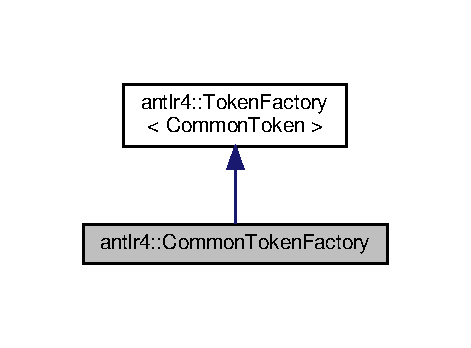
\includegraphics[width=226pt]{classantlr4_1_1CommonTokenFactory__inherit__graph}
\end{center}
\end{figure}


Collaboration diagram for antlr4\+:\+:Common\+Token\+Factory\+:
\nopagebreak
\begin{figure}[H]
\begin{center}
\leavevmode
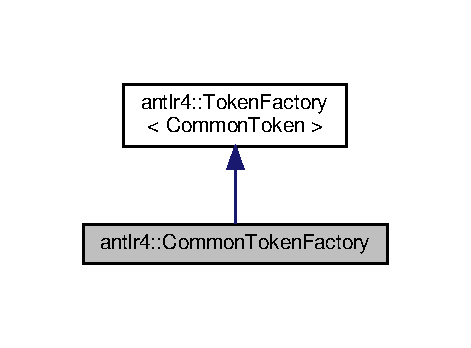
\includegraphics[width=226pt]{classantlr4_1_1CommonTokenFactory__coll__graph}
\end{center}
\end{figure}
\subsection*{Public Member Functions}
\begin{DoxyCompactItemize}
\item 
\hyperlink{classantlr4_1_1CommonTokenFactory_a580c068f46164c58052858432bbf974c}{Common\+Token\+Factory} (bool \hyperlink{classantlr4_1_1CommonTokenFactory_a944c106da2cf4638ea989bcb20b482df}{copy\+Text})
\item 
\hyperlink{classantlr4_1_1CommonTokenFactory_a4bf0a30d96f0239d56c72d0b5dc634f7}{Common\+Token\+Factory} ()
\item 
virtual std\+::unique\+\_\+ptr$<$ \hyperlink{classantlr4_1_1CommonToken}{Common\+Token} $>$ \hyperlink{classantlr4_1_1CommonTokenFactory_ae5b0ee244ce69cf24a71c81167328be1}{create} (std\+::pair$<$ \hyperlink{classantlr4_1_1TokenSource}{Token\+Source} $\ast$, Char\+Stream $\ast$$>$ source, size\+\_\+t type, const std\+::string \&text, size\+\_\+t channel, size\+\_\+t start, size\+\_\+t stop, size\+\_\+t line, size\+\_\+t char\+Position\+In\+Line) override
\item 
\mbox{\Hypertarget{classantlr4_1_1CommonTokenFactory_a9b21aad910d0976a291c7b4aed688aad}\label{classantlr4_1_1CommonTokenFactory_a9b21aad910d0976a291c7b4aed688aad}} 
virtual std\+::unique\+\_\+ptr$<$ \hyperlink{classantlr4_1_1CommonToken}{Common\+Token} $>$ \hyperlink{classantlr4_1_1CommonTokenFactory_a9b21aad910d0976a291c7b4aed688aad}{create} (size\+\_\+t type, const std\+::string \&text) override
\begin{DoxyCompactList}\small\item\em Generically useful. \end{DoxyCompactList}\end{DoxyCompactItemize}
\subsection*{Static Public Attributes}
\begin{DoxyCompactItemize}
\item 
static const Ref$<$ \hyperlink{classantlr4_1_1TokenFactory}{Token\+Factory}$<$ \hyperlink{classantlr4_1_1CommonToken}{Common\+Token} $>$ $>$ \hyperlink{classantlr4_1_1CommonTokenFactory_a141e9716e14a7b5c43a6d0bd3db82bcd}{D\+E\+F\+A\+U\+LT} = std\+::make\+\_\+shared$<$\hyperlink{classantlr4_1_1CommonTokenFactory}{Common\+Token\+Factory}$>$()
\end{DoxyCompactItemize}
\subsection*{Protected Attributes}
\begin{DoxyCompactItemize}
\item 
const bool \hyperlink{classantlr4_1_1CommonTokenFactory_a944c106da2cf4638ea989bcb20b482df}{copy\+Text}
\end{DoxyCompactItemize}


\subsection{Detailed Description}
This default implementation of \hyperlink{classantlr4_1_1TokenFactory}{Token\+Factory} creates \hyperlink{classantlr4_1_1CommonToken}{Common\+Token} objects. 

\subsection{Constructor \& Destructor Documentation}
\mbox{\Hypertarget{classantlr4_1_1CommonTokenFactory_a580c068f46164c58052858432bbf974c}\label{classantlr4_1_1CommonTokenFactory_a580c068f46164c58052858432bbf974c}} 
\index{antlr4\+::\+Common\+Token\+Factory@{antlr4\+::\+Common\+Token\+Factory}!Common\+Token\+Factory@{Common\+Token\+Factory}}
\index{Common\+Token\+Factory@{Common\+Token\+Factory}!antlr4\+::\+Common\+Token\+Factory@{antlr4\+::\+Common\+Token\+Factory}}
\subsubsection{\texorpdfstring{Common\+Token\+Factory()}{CommonTokenFactory()}\hspace{0.1cm}{\footnotesize\ttfamily [1/2]}}
{\footnotesize\ttfamily Common\+Token\+Factory\+::\+Common\+Token\+Factory (\begin{DoxyParamCaption}\item[{bool}]{copy\+Text }\end{DoxyParamCaption})}

Constructs a \hyperlink{classantlr4_1_1CommonTokenFactory}{Common\+Token\+Factory} with the specified value for \hyperlink{classantlr4_1_1CommonTokenFactory_a944c106da2cf4638ea989bcb20b482df}{copy\+Text}.

When
\begin{DoxyCode}
\hyperlink{classantlr4_1_1CommonTokenFactory_a944c106da2cf4638ea989bcb20b482df}{copyText} 
\end{DoxyCode}
 is
\begin{DoxyCode}
\textcolor{keyword}{false} 
\end{DoxyCode}
 , the \hyperlink{classantlr4_1_1CommonTokenFactory_a141e9716e14a7b5c43a6d0bd3db82bcd}{D\+E\+F\+A\+U\+LT} instance should be used instead of constructing a new instance.


\begin{DoxyParams}{Parameters}
{\em copy\+Text} & The value for \hyperlink{classantlr4_1_1CommonTokenFactory_a944c106da2cf4638ea989bcb20b482df}{copy\+Text}. \\
\hline
\end{DoxyParams}
\mbox{\Hypertarget{classantlr4_1_1CommonTokenFactory_a4bf0a30d96f0239d56c72d0b5dc634f7}\label{classantlr4_1_1CommonTokenFactory_a4bf0a30d96f0239d56c72d0b5dc634f7}} 
\index{antlr4\+::\+Common\+Token\+Factory@{antlr4\+::\+Common\+Token\+Factory}!Common\+Token\+Factory@{Common\+Token\+Factory}}
\index{Common\+Token\+Factory@{Common\+Token\+Factory}!antlr4\+::\+Common\+Token\+Factory@{antlr4\+::\+Common\+Token\+Factory}}
\subsubsection{\texorpdfstring{Common\+Token\+Factory()}{CommonTokenFactory()}\hspace{0.1cm}{\footnotesize\ttfamily [2/2]}}
{\footnotesize\ttfamily Common\+Token\+Factory\+::\+Common\+Token\+Factory (\begin{DoxyParamCaption}{ }\end{DoxyParamCaption})}

Constructs a \hyperlink{classantlr4_1_1CommonTokenFactory}{Common\+Token\+Factory} with \hyperlink{classantlr4_1_1CommonTokenFactory_a944c106da2cf4638ea989bcb20b482df}{copy\+Text} set to 
\begin{DoxyCode}
\textcolor{keyword}{false} 
\end{DoxyCode}
 .

The \hyperlink{classantlr4_1_1CommonTokenFactory_a141e9716e14a7b5c43a6d0bd3db82bcd}{D\+E\+F\+A\+U\+LT} instance should be used instead of calling this directly.

\subsection{Member Function Documentation}
\mbox{\Hypertarget{classantlr4_1_1CommonTokenFactory_ae5b0ee244ce69cf24a71c81167328be1}\label{classantlr4_1_1CommonTokenFactory_ae5b0ee244ce69cf24a71c81167328be1}} 
\index{antlr4\+::\+Common\+Token\+Factory@{antlr4\+::\+Common\+Token\+Factory}!create@{create}}
\index{create@{create}!antlr4\+::\+Common\+Token\+Factory@{antlr4\+::\+Common\+Token\+Factory}}
\subsubsection{\texorpdfstring{create()}{create()}}
{\footnotesize\ttfamily std\+::unique\+\_\+ptr$<$ \hyperlink{classantlr4_1_1CommonToken}{Common\+Token} $>$ Common\+Token\+Factory\+::create (\begin{DoxyParamCaption}\item[{std\+::pair$<$ \hyperlink{classantlr4_1_1TokenSource}{Token\+Source} $\ast$, Char\+Stream $\ast$$>$}]{source,  }\item[{size\+\_\+t}]{type,  }\item[{const std\+::string \&}]{text,  }\item[{size\+\_\+t}]{channel,  }\item[{size\+\_\+t}]{start,  }\item[{size\+\_\+t}]{stop,  }\item[{size\+\_\+t}]{line,  }\item[{size\+\_\+t}]{char\+Position\+In\+Line }\end{DoxyParamCaption})\hspace{0.3cm}{\ttfamily [override]}, {\ttfamily [virtual]}}

This is the method used to create tokens in the lexer and in the error handling strategy. If text!=null, than the start and stop positions are wiped to -\/1 in the text override is set in the \hyperlink{classantlr4_1_1CommonToken}{Common\+Token}. 

Implements \hyperlink{classantlr4_1_1TokenFactory_a25efd6b38907e594ddc848887fbd7303}{antlr4\+::\+Token\+Factory$<$ Common\+Token $>$}.



\subsection{Member Data Documentation}
\mbox{\Hypertarget{classantlr4_1_1CommonTokenFactory_a944c106da2cf4638ea989bcb20b482df}\label{classantlr4_1_1CommonTokenFactory_a944c106da2cf4638ea989bcb20b482df}} 
\index{antlr4\+::\+Common\+Token\+Factory@{antlr4\+::\+Common\+Token\+Factory}!copy\+Text@{copy\+Text}}
\index{copy\+Text@{copy\+Text}!antlr4\+::\+Common\+Token\+Factory@{antlr4\+::\+Common\+Token\+Factory}}
\subsubsection{\texorpdfstring{copy\+Text}{copyText}}
{\footnotesize\ttfamily const bool antlr4\+::\+Common\+Token\+Factory\+::copy\+Text\hspace{0.3cm}{\ttfamily [protected]}}

Indicates whether \hyperlink{classantlr4_1_1CommonToken_a2963f31fa12fdb1c5c26711004177554}{Common\+Token\#set\+Text} should be called after constructing tokens to explicitly set the text. This is useful for cases where the input stream might not be able to provide arbitrary substrings of text from the input after the lexer creates a token (e.\+g. the implementation of \hyperlink{}{Char\+Stream\#get\+Text} in \hyperlink{}{Unbuffered\+Char\+Stream} throws an \hyperlink{classantlr4_1_1UnsupportedOperationException}{Unsupported\+Operation\+Exception}). Explicitly setting the token text allows \hyperlink{classantlr4_1_1Token_ae288d9f2d72d0209a24e0cc5215e8844}{Token\#get\+Text} to be called at any time regardless of the input stream implementation.

The default value is
\begin{DoxyCode}
\textcolor{keyword}{false} 
\end{DoxyCode}
 to avoid the performance and memory overhead of copying text for every token unless explicitly requested.\mbox{\Hypertarget{classantlr4_1_1CommonTokenFactory_a141e9716e14a7b5c43a6d0bd3db82bcd}\label{classantlr4_1_1CommonTokenFactory_a141e9716e14a7b5c43a6d0bd3db82bcd}} 
\index{antlr4\+::\+Common\+Token\+Factory@{antlr4\+::\+Common\+Token\+Factory}!D\+E\+F\+A\+U\+LT@{D\+E\+F\+A\+U\+LT}}
\index{D\+E\+F\+A\+U\+LT@{D\+E\+F\+A\+U\+LT}!antlr4\+::\+Common\+Token\+Factory@{antlr4\+::\+Common\+Token\+Factory}}
\subsubsection{\texorpdfstring{D\+E\+F\+A\+U\+LT}{DEFAULT}}
{\footnotesize\ttfamily const Ref$<$ \hyperlink{classantlr4_1_1TokenFactory}{Token\+Factory}$<$ \hyperlink{classantlr4_1_1CommonToken}{Common\+Token} $>$ $>$ Common\+Token\+Factory\+::\+D\+E\+F\+A\+U\+LT = std\+::make\+\_\+shared$<$\hyperlink{classantlr4_1_1CommonTokenFactory}{Common\+Token\+Factory}$>$()\hspace{0.3cm}{\ttfamily [static]}}

The default \hyperlink{classantlr4_1_1CommonTokenFactory}{Common\+Token\+Factory} instance.

This token factory does not explicitly copy token text when constructing tokens.

The documentation for this class was generated from the following files\+:\begin{DoxyCompactItemize}
\item 
Common\+Token\+Factory.\+h\item 
Common\+Token\+Factory.\+cpp\end{DoxyCompactItemize}

\hypertarget{classantlr4_1_1CommonTokenStream}{}\section{antlr4\+:\+:Common\+Token\+Stream Class Reference}
\label{classantlr4_1_1CommonTokenStream}\index{antlr4\+::\+Common\+Token\+Stream@{antlr4\+::\+Common\+Token\+Stream}}


{\ttfamily \#include $<$Common\+Token\+Stream.\+h$>$}



Inheritance diagram for antlr4\+:\+:Common\+Token\+Stream\+:
\nopagebreak
\begin{figure}[H]
\begin{center}
\leavevmode
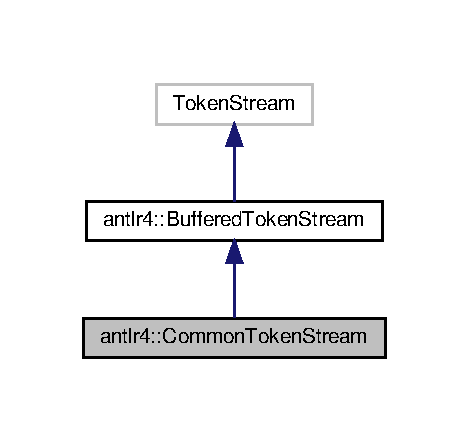
\includegraphics[width=225pt]{classantlr4_1_1CommonTokenStream__inherit__graph}
\end{center}
\end{figure}


Collaboration diagram for antlr4\+:\+:Common\+Token\+Stream\+:
\nopagebreak
\begin{figure}[H]
\begin{center}
\leavevmode
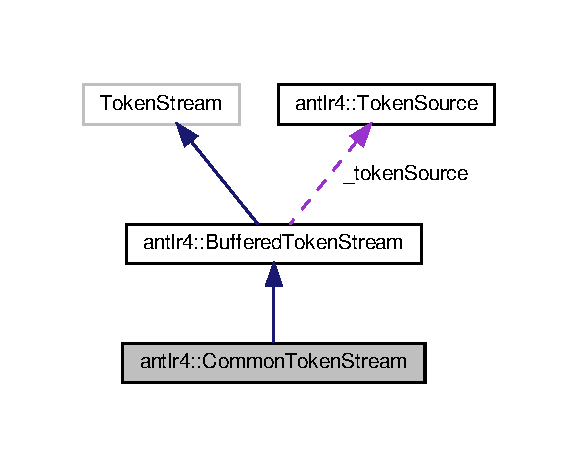
\includegraphics[width=278pt]{classantlr4_1_1CommonTokenStream__coll__graph}
\end{center}
\end{figure}
\subsection*{Public Member Functions}
\begin{DoxyCompactItemize}
\item 
\hyperlink{classantlr4_1_1CommonTokenStream_a70ef318ad41bc2f99f44549027f886e1}{Common\+Token\+Stream} (\hyperlink{classantlr4_1_1TokenSource}{Token\+Source} $\ast$token\+Source)
\item 
\hyperlink{classantlr4_1_1CommonTokenStream_a3565e4d1910fb5e13b49d6a1f12e5cd7}{Common\+Token\+Stream} (\hyperlink{classantlr4_1_1TokenSource}{Token\+Source} $\ast$token\+Source, size\+\_\+t \hyperlink{classantlr4_1_1CommonTokenStream_aad59d04a125961d8ba1cffdf4a1a0bcf}{channel})
\item 
\mbox{\Hypertarget{classantlr4_1_1CommonTokenStream_ab92b8381589e1a5aacf6e7ffdcf89dfc}\label{classantlr4_1_1CommonTokenStream_ab92b8381589e1a5aacf6e7ffdcf89dfc}} 
virtual \hyperlink{classantlr4_1_1Token}{Token} $\ast$ {\bfseries LT} (ssize\+\_\+t k) override
\item 
\mbox{\Hypertarget{classantlr4_1_1CommonTokenStream_aafecb98aeb51496b59bc3bb19e228128}\label{classantlr4_1_1CommonTokenStream_aafecb98aeb51496b59bc3bb19e228128}} 
virtual int \hyperlink{classantlr4_1_1CommonTokenStream_aafecb98aeb51496b59bc3bb19e228128}{get\+Number\+Of\+On\+Channel\+Tokens} ()
\begin{DoxyCompactList}\small\item\em Count E\+OF just once. \end{DoxyCompactList}\end{DoxyCompactItemize}
\subsection*{Protected Member Functions}
\begin{DoxyCompactItemize}
\item 
\mbox{\Hypertarget{classantlr4_1_1CommonTokenStream_a5b8a9ff0beab08b379df20c5306b98cc}\label{classantlr4_1_1CommonTokenStream_a5b8a9ff0beab08b379df20c5306b98cc}} 
virtual ssize\+\_\+t {\bfseries adjust\+Seek\+Index} (size\+\_\+t i) override
\item 
\mbox{\Hypertarget{classantlr4_1_1CommonTokenStream_a2efe72e48498674a5db9d664aaea9d65}\label{classantlr4_1_1CommonTokenStream_a2efe72e48498674a5db9d664aaea9d65}} 
virtual \hyperlink{classantlr4_1_1Token}{Token} $\ast$ {\bfseries LB} (size\+\_\+t k) override
\end{DoxyCompactItemize}
\subsection*{Protected Attributes}
\begin{DoxyCompactItemize}
\item 
size\+\_\+t \hyperlink{classantlr4_1_1CommonTokenStream_aad59d04a125961d8ba1cffdf4a1a0bcf}{channel}
\end{DoxyCompactItemize}


\subsection{Detailed Description}
This class extends \hyperlink{classantlr4_1_1BufferedTokenStream}{Buffered\+Token\+Stream} with functionality to filter token streams to tokens on a particular channel (tokens where \hyperlink{classantlr4_1_1Token_a92991c0566e4cb00ae2c5f9e7d8fe6b4}{Token\#get\+Channel} returns a particular value).

This token stream provides access to all tokens by index or when calling methods like \hyperlink{}{get\+Text}. The channel filtering is only used for code accessing tokens via the lookahead methods \hyperlink{}{LA}, \hyperlink{}{LT}, and \hyperlink{}{LB}.

By default, tokens are placed on the default channel (\hyperlink{classantlr4_1_1Token_a699cbc56affbddc079561e175cba8435}{Token\#\+D\+E\+F\+A\+U\+L\+T\+\_\+\+C\+H\+A\+N\+N\+EL}), but may be reassigned by using the 
\begin{DoxyCode}
->channel(HIDDEN) 
\end{DoxyCode}
 lexer command, or by using an embedded action to call \hyperlink{}{Lexer\#set\+Channel}. 

Note\+: lexer rules which use the
\begin{DoxyCode}
->skip 
\end{DoxyCode}
 lexer command or call \hyperlink{classantlr4_1_1Lexer_a8d2585d70adce01584a505a25c3e179d}{Lexer\#skip} do not produce tokens at all, so input text matched by such a rule will not be available as part of the token stream, regardless of channel.

\subsection{Constructor \& Destructor Documentation}
\mbox{\Hypertarget{classantlr4_1_1CommonTokenStream_a70ef318ad41bc2f99f44549027f886e1}\label{classantlr4_1_1CommonTokenStream_a70ef318ad41bc2f99f44549027f886e1}} 
\index{antlr4\+::\+Common\+Token\+Stream@{antlr4\+::\+Common\+Token\+Stream}!Common\+Token\+Stream@{Common\+Token\+Stream}}
\index{Common\+Token\+Stream@{Common\+Token\+Stream}!antlr4\+::\+Common\+Token\+Stream@{antlr4\+::\+Common\+Token\+Stream}}
\subsubsection{\texorpdfstring{Common\+Token\+Stream()}{CommonTokenStream()}\hspace{0.1cm}{\footnotesize\ttfamily [1/2]}}
{\footnotesize\ttfamily Common\+Token\+Stream\+::\+Common\+Token\+Stream (\begin{DoxyParamCaption}\item[{\hyperlink{classantlr4_1_1TokenSource}{Token\+Source} $\ast$}]{token\+Source }\end{DoxyParamCaption})}

Constructs a new \hyperlink{classantlr4_1_1CommonTokenStream}{Common\+Token\+Stream} using the specified token source and the default token channel (\hyperlink{classantlr4_1_1Token_a699cbc56affbddc079561e175cba8435}{Token\#\+D\+E\+F\+A\+U\+L\+T\+\_\+\+C\+H\+A\+N\+N\+EL}).


\begin{DoxyParams}{Parameters}
{\em token\+Source} & The token source. \\
\hline
\end{DoxyParams}
\mbox{\Hypertarget{classantlr4_1_1CommonTokenStream_a3565e4d1910fb5e13b49d6a1f12e5cd7}\label{classantlr4_1_1CommonTokenStream_a3565e4d1910fb5e13b49d6a1f12e5cd7}} 
\index{antlr4\+::\+Common\+Token\+Stream@{antlr4\+::\+Common\+Token\+Stream}!Common\+Token\+Stream@{Common\+Token\+Stream}}
\index{Common\+Token\+Stream@{Common\+Token\+Stream}!antlr4\+::\+Common\+Token\+Stream@{antlr4\+::\+Common\+Token\+Stream}}
\subsubsection{\texorpdfstring{Common\+Token\+Stream()}{CommonTokenStream()}\hspace{0.1cm}{\footnotesize\ttfamily [2/2]}}
{\footnotesize\ttfamily Common\+Token\+Stream\+::\+Common\+Token\+Stream (\begin{DoxyParamCaption}\item[{\hyperlink{classantlr4_1_1TokenSource}{Token\+Source} $\ast$}]{token\+Source,  }\item[{size\+\_\+t}]{channel }\end{DoxyParamCaption})}

Constructs a new \hyperlink{classantlr4_1_1CommonTokenStream}{Common\+Token\+Stream} using the specified token source and filtering tokens to the specified channel. Only tokens whose \hyperlink{classantlr4_1_1Token_a92991c0566e4cb00ae2c5f9e7d8fe6b4}{Token\#get\+Channel} matches
\begin{DoxyCode}
\hyperlink{classantlr4_1_1CommonTokenStream_aad59d04a125961d8ba1cffdf4a1a0bcf}{channel} 
\end{DoxyCode}
 or have the \hyperlink{classantlr4_1_1Token_a518342431db9dd9d982880a59ef0e4f4}{Token\#get\+Type} equal to \hyperlink{}{Token\#\+E\+OF} will be returned by the token stream lookahead methods.


\begin{DoxyParams}{Parameters}
{\em token\+Source} & The token source. \\
\hline
{\em channel} & The channel to use for filtering tokens. \\
\hline
\end{DoxyParams}


\subsection{Member Data Documentation}
\mbox{\Hypertarget{classantlr4_1_1CommonTokenStream_aad59d04a125961d8ba1cffdf4a1a0bcf}\label{classantlr4_1_1CommonTokenStream_aad59d04a125961d8ba1cffdf4a1a0bcf}} 
\index{antlr4\+::\+Common\+Token\+Stream@{antlr4\+::\+Common\+Token\+Stream}!channel@{channel}}
\index{channel@{channel}!antlr4\+::\+Common\+Token\+Stream@{antlr4\+::\+Common\+Token\+Stream}}
\subsubsection{\texorpdfstring{channel}{channel}}
{\footnotesize\ttfamily size\+\_\+t antlr4\+::\+Common\+Token\+Stream\+::channel\hspace{0.3cm}{\ttfamily [protected]}}

Specifies the channel to use for filtering tokens.

The default value is \hyperlink{classantlr4_1_1Token_a699cbc56affbddc079561e175cba8435}{Token\#\+D\+E\+F\+A\+U\+L\+T\+\_\+\+C\+H\+A\+N\+N\+EL}, which matches the default channel assigned to tokens created by the lexer.

The documentation for this class was generated from the following files\+:\begin{DoxyCompactItemize}
\item 
Common\+Token\+Stream.\+h\item 
Common\+Token\+Stream.\+cpp\end{DoxyCompactItemize}

\hypertarget{structantlr4_1_1atn_1_1ATNConfig_1_1Comparer}{}\section{antlr4\+:\+:atn\+:\+:A\+T\+N\+Config\+:\+:Comparer Struct Reference}
\label{structantlr4_1_1atn_1_1ATNConfig_1_1Comparer}\index{antlr4\+::atn\+::\+A\+T\+N\+Config\+::\+Comparer@{antlr4\+::atn\+::\+A\+T\+N\+Config\+::\+Comparer}}
\subsection*{Public Member Functions}
\begin{DoxyCompactItemize}
\item 
\mbox{\Hypertarget{structantlr4_1_1atn_1_1ATNConfig_1_1Comparer_a9c1ad13718f8e276422d1a6eaad0a3d2}\label{structantlr4_1_1atn_1_1ATNConfig_1_1Comparer_a9c1ad13718f8e276422d1a6eaad0a3d2}} 
bool {\bfseries operator()} (\hyperlink{classantlr4_1_1atn_1_1ATNConfig}{A\+T\+N\+Config} const \&lhs, \hyperlink{classantlr4_1_1atn_1_1ATNConfig}{A\+T\+N\+Config} const \&rhs) const
\end{DoxyCompactItemize}


The documentation for this struct was generated from the following file\+:\begin{DoxyCompactItemize}
\item 
atn/A\+T\+N\+Config.\+h\end{DoxyCompactItemize}

\hypertarget{structantlr4_1_1atn_1_1SemanticContext_1_1Comparer}{}\section{antlr4\+:\+:atn\+:\+:Semantic\+Context\+:\+:Comparer Struct Reference}
\label{structantlr4_1_1atn_1_1SemanticContext_1_1Comparer}\index{antlr4\+::atn\+::\+Semantic\+Context\+::\+Comparer@{antlr4\+::atn\+::\+Semantic\+Context\+::\+Comparer}}
\subsection*{Public Member Functions}
\begin{DoxyCompactItemize}
\item 
\mbox{\Hypertarget{structantlr4_1_1atn_1_1SemanticContext_1_1Comparer_a3b881e913bdb47f3e7bcfb833533c3f9}\label{structantlr4_1_1atn_1_1SemanticContext_1_1Comparer_a3b881e913bdb47f3e7bcfb833533c3f9}} 
bool {\bfseries operator()} (Ref$<$ \hyperlink{classantlr4_1_1atn_1_1SemanticContext}{Semantic\+Context} $>$ const \&lhs, Ref$<$ \hyperlink{classantlr4_1_1atn_1_1SemanticContext}{Semantic\+Context} $>$ const \&rhs) const
\end{DoxyCompactItemize}


The documentation for this struct was generated from the following file\+:\begin{DoxyCompactItemize}
\item 
atn/Semantic\+Context.\+h\end{DoxyCompactItemize}

\hypertarget{classantlr4_1_1ConsoleErrorListener}{}\section{antlr4\+:\+:Console\+Error\+Listener Class Reference}
\label{classantlr4_1_1ConsoleErrorListener}\index{antlr4\+::\+Console\+Error\+Listener@{antlr4\+::\+Console\+Error\+Listener}}


Inheritance diagram for antlr4\+:\+:Console\+Error\+Listener\+:
\nopagebreak
\begin{figure}[H]
\begin{center}
\leavevmode
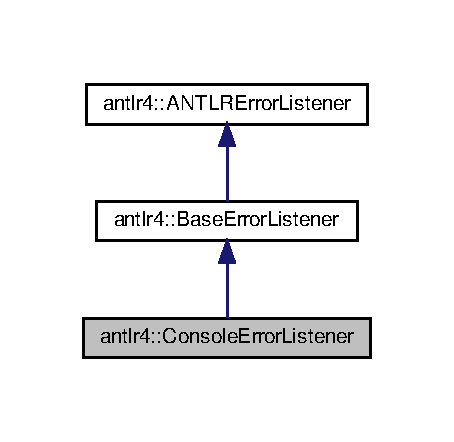
\includegraphics[width=218pt]{classantlr4_1_1ConsoleErrorListener__inherit__graph}
\end{center}
\end{figure}


Collaboration diagram for antlr4\+:\+:Console\+Error\+Listener\+:
\nopagebreak
\begin{figure}[H]
\begin{center}
\leavevmode
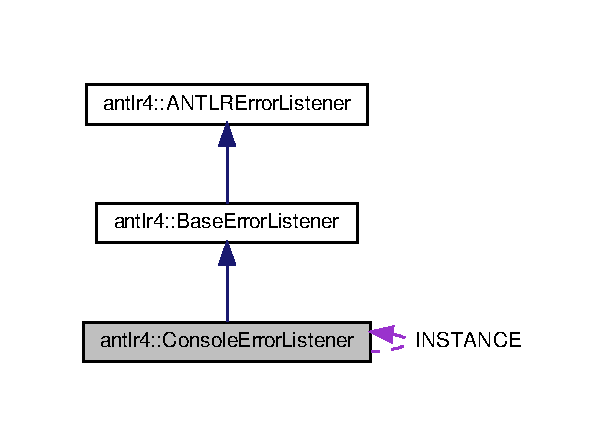
\includegraphics[width=291pt]{classantlr4_1_1ConsoleErrorListener__coll__graph}
\end{center}
\end{figure}
\subsection*{Public Member Functions}
\begin{DoxyCompactItemize}
\item 
virtual void \hyperlink{classantlr4_1_1ConsoleErrorListener_ac8ba720010f28a83cae7c150c6f1775b}{syntax\+Error} (\hyperlink{classantlr4_1_1Recognizer}{Recognizer} $\ast$recognizer, \hyperlink{classantlr4_1_1Token}{Token} $\ast$offending\+Symbol, size\+\_\+t line, size\+\_\+t char\+Position\+In\+Line, const std\+::string \&msg, std\+::exception\+\_\+ptr e) override
\end{DoxyCompactItemize}
\subsection*{Static Public Attributes}
\begin{DoxyCompactItemize}
\item 
static \hyperlink{classantlr4_1_1ConsoleErrorListener}{Console\+Error\+Listener} \hyperlink{classantlr4_1_1ConsoleErrorListener_a61b93f6c4f075888001972f35698d5ff}{I\+N\+S\+T\+A\+N\+CE}
\end{DoxyCompactItemize}


\subsection{Member Function Documentation}
\mbox{\Hypertarget{classantlr4_1_1ConsoleErrorListener_ac8ba720010f28a83cae7c150c6f1775b}\label{classantlr4_1_1ConsoleErrorListener_ac8ba720010f28a83cae7c150c6f1775b}} 
\index{antlr4\+::\+Console\+Error\+Listener@{antlr4\+::\+Console\+Error\+Listener}!syntax\+Error@{syntax\+Error}}
\index{syntax\+Error@{syntax\+Error}!antlr4\+::\+Console\+Error\+Listener@{antlr4\+::\+Console\+Error\+Listener}}
\subsubsection{\texorpdfstring{syntax\+Error()}{syntaxError()}}
{\footnotesize\ttfamily void Console\+Error\+Listener\+::syntax\+Error (\begin{DoxyParamCaption}\item[{\hyperlink{classantlr4_1_1Recognizer}{Recognizer} $\ast$}]{recognizer,  }\item[{\hyperlink{classantlr4_1_1Token}{Token} $\ast$}]{offending\+Symbol,  }\item[{size\+\_\+t}]{line,  }\item[{size\+\_\+t}]{char\+Position\+In\+Line,  }\item[{const std\+::string \&}]{msg,  }\item[{std\+::exception\+\_\+ptr}]{e }\end{DoxyParamCaption})\hspace{0.3cm}{\ttfamily [override]}, {\ttfamily [virtual]}}

This implementation prints messages to \hyperlink{}{System\#err} containing the values of
\begin{DoxyCode}
line 
\end{DoxyCode}
 ,
\begin{DoxyCode}
charPositionInLine 
\end{DoxyCode}
 , and
\begin{DoxyCode}
msg 
\end{DoxyCode}
 using the following format.


\begin{DoxyPre}
line {\itshape line}:{\itshape charPositionInLine} {\itshape msg}
\end{DoxyPre}
 

Reimplemented from \hyperlink{classantlr4_1_1BaseErrorListener}{antlr4\+::\+Base\+Error\+Listener}.



\subsection{Member Data Documentation}
\mbox{\Hypertarget{classantlr4_1_1ConsoleErrorListener_a61b93f6c4f075888001972f35698d5ff}\label{classantlr4_1_1ConsoleErrorListener_a61b93f6c4f075888001972f35698d5ff}} 
\index{antlr4\+::\+Console\+Error\+Listener@{antlr4\+::\+Console\+Error\+Listener}!I\+N\+S\+T\+A\+N\+CE@{I\+N\+S\+T\+A\+N\+CE}}
\index{I\+N\+S\+T\+A\+N\+CE@{I\+N\+S\+T\+A\+N\+CE}!antlr4\+::\+Console\+Error\+Listener@{antlr4\+::\+Console\+Error\+Listener}}
\subsubsection{\texorpdfstring{I\+N\+S\+T\+A\+N\+CE}{INSTANCE}}
{\footnotesize\ttfamily \hyperlink{classantlr4_1_1ConsoleErrorListener}{Console\+Error\+Listener} Console\+Error\+Listener\+::\+I\+N\+S\+T\+A\+N\+CE\hspace{0.3cm}{\ttfamily [static]}}

Provides a default instance of \hyperlink{classantlr4_1_1ConsoleErrorListener}{Console\+Error\+Listener}. 

The documentation for this class was generated from the following files\+:\begin{DoxyCompactItemize}
\item 
Console\+Error\+Listener.\+h\item 
Console\+Error\+Listener.\+cpp\end{DoxyCompactItemize}

\hypertarget{classantlr4_1_1atn_1_1ContextSensitivityInfo}{}\section{antlr4\+:\+:atn\+:\+:Context\+Sensitivity\+Info Class Reference}
\label{classantlr4_1_1atn_1_1ContextSensitivityInfo}\index{antlr4\+::atn\+::\+Context\+Sensitivity\+Info@{antlr4\+::atn\+::\+Context\+Sensitivity\+Info}}


This class represents profiling event information for a context sensitivity. Context sensitivities are decisions where a particular input resulted in an S\+LL conflict, but LL prediction produced a single unique alternative.  




{\ttfamily \#include $<$Context\+Sensitivity\+Info.\+h$>$}



Inheritance diagram for antlr4\+:\+:atn\+:\+:Context\+Sensitivity\+Info\+:
\nopagebreak
\begin{figure}[H]
\begin{center}
\leavevmode
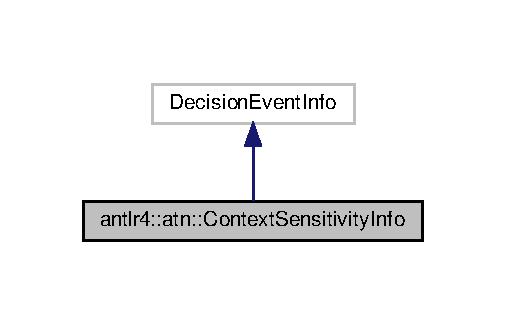
\includegraphics[width=243pt]{classantlr4_1_1atn_1_1ContextSensitivityInfo__inherit__graph}
\end{center}
\end{figure}


Collaboration diagram for antlr4\+:\+:atn\+:\+:Context\+Sensitivity\+Info\+:
\nopagebreak
\begin{figure}[H]
\begin{center}
\leavevmode
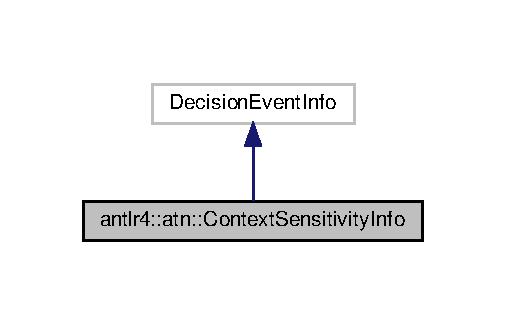
\includegraphics[width=243pt]{classantlr4_1_1atn_1_1ContextSensitivityInfo__coll__graph}
\end{center}
\end{figure}
\subsection*{Public Member Functions}
\begin{DoxyCompactItemize}
\item 
\hyperlink{classantlr4_1_1atn_1_1ContextSensitivityInfo_a900c044cd1a49de278001c48d02898cf}{Context\+Sensitivity\+Info} (size\+\_\+t decision, \hyperlink{classantlr4_1_1atn_1_1ATNConfigSet}{A\+T\+N\+Config\+Set} $\ast$configs, Token\+Stream $\ast$input, size\+\_\+t start\+Index, size\+\_\+t stop\+Index)
\begin{DoxyCompactList}\small\item\em Constructs a new instance of the \begin{DoxySeeAlso}{See also}
\hyperlink{classantlr4_1_1atn_1_1ContextSensitivityInfo}{Context\+Sensitivity\+Info}


\end{DoxySeeAlso}
class with the specified detailed context sensitivity information. \end{DoxyCompactList}\end{DoxyCompactItemize}


\subsection{Detailed Description}
This class represents profiling event information for a context sensitivity. Context sensitivities are decisions where a particular input resulted in an S\+LL conflict, but LL prediction produced a single unique alternative. 

In some cases, the unique alternative identified by LL prediction is not equal to the minimum represented alternative in the conflicting S\+LL configuration set. Grammars and inputs which result in this scenario are unable to use \begin{DoxySeeAlso}{See also}
Prediction\+Mode\+::\+S\+LL


\end{DoxySeeAlso}
, which in turn means they cannot use the two-\/stage parsing strategy to improve parsing performance for that input.

$<$seealso cref= Parser\+A\+T\+N\+Simulator\+::report\+Context\+Sensitivity 

$<$seealso cref= A\+N\+T\+L\+R\+Error\+Listener\+::report\+Context\+Sensitivity

\begin{DoxySince}{Since}
4.\+3 
\end{DoxySince}


\subsection{Constructor \& Destructor Documentation}
\mbox{\Hypertarget{classantlr4_1_1atn_1_1ContextSensitivityInfo_a900c044cd1a49de278001c48d02898cf}\label{classantlr4_1_1atn_1_1ContextSensitivityInfo_a900c044cd1a49de278001c48d02898cf}} 
\index{antlr4\+::atn\+::\+Context\+Sensitivity\+Info@{antlr4\+::atn\+::\+Context\+Sensitivity\+Info}!Context\+Sensitivity\+Info@{Context\+Sensitivity\+Info}}
\index{Context\+Sensitivity\+Info@{Context\+Sensitivity\+Info}!antlr4\+::atn\+::\+Context\+Sensitivity\+Info@{antlr4\+::atn\+::\+Context\+Sensitivity\+Info}}
\subsubsection{\texorpdfstring{Context\+Sensitivity\+Info()}{ContextSensitivityInfo()}}
{\footnotesize\ttfamily Context\+Sensitivity\+Info\+::\+Context\+Sensitivity\+Info (\begin{DoxyParamCaption}\item[{size\+\_\+t}]{decision,  }\item[{\hyperlink{classantlr4_1_1atn_1_1ATNConfigSet}{A\+T\+N\+Config\+Set} $\ast$}]{configs,  }\item[{Token\+Stream $\ast$}]{input,  }\item[{size\+\_\+t}]{start\+Index,  }\item[{size\+\_\+t}]{stop\+Index }\end{DoxyParamCaption})}



Constructs a new instance of the \begin{DoxySeeAlso}{See also}
\hyperlink{classantlr4_1_1atn_1_1ContextSensitivityInfo}{Context\+Sensitivity\+Info}


\end{DoxySeeAlso}
class with the specified detailed context sensitivity information. 


\begin{DoxyParams}{Parameters}
{\em decision} & The decision number \\
\hline
{\em configs} & The final configuration set containing the unique alternative identified by full-\/context prediction \\
\hline
{\em input} & The input token stream \\
\hline
{\em start\+Index} & The start index for the current prediction \\
\hline
{\em stop\+Index} & The index at which the context sensitivity was identified during full-\/context prediction \\
\hline
\end{DoxyParams}


The documentation for this class was generated from the following files\+:\begin{DoxyCompactItemize}
\item 
atn/Context\+Sensitivity\+Info.\+h\item 
atn/Context\+Sensitivity\+Info.\+cpp\end{DoxyCompactItemize}

\hypertarget{classantlr4_1_1atn_1_1DecisionInfo}{}\section{antlr4\+:\+:atn\+:\+:Decision\+Info Class Reference}
\label{classantlr4_1_1atn_1_1DecisionInfo}\index{antlr4\+::atn\+::\+Decision\+Info@{antlr4\+::atn\+::\+Decision\+Info}}


This class contains profiling gathered for a particular decision.  




{\ttfamily \#include $<$Decision\+Info.\+h$>$}

\subsection*{Public Member Functions}
\begin{DoxyCompactItemize}
\item 
\hyperlink{classantlr4_1_1atn_1_1DecisionInfo_a99833736f88c09563a01b57284742b88}{Decision\+Info} (size\+\_\+t \hyperlink{classantlr4_1_1atn_1_1DecisionInfo_ad81f14a210fb5e80f86ac800d56cc7bb}{decision})
\begin{DoxyCompactList}\small\item\em Constructs a new instance of the \begin{DoxySeeAlso}{See also}
\hyperlink{classantlr4_1_1atn_1_1DecisionInfo}{Decision\+Info}


\end{DoxySeeAlso}
class to contain statistics for a particular decision. \end{DoxyCompactList}\item 
\mbox{\Hypertarget{classantlr4_1_1atn_1_1DecisionInfo_a20a4ba0dfbd5e17526e7e6e6e888616d}\label{classantlr4_1_1atn_1_1DecisionInfo_a20a4ba0dfbd5e17526e7e6e6e888616d}} 
std\+::string {\bfseries to\+String} () const
\end{DoxyCompactItemize}
\subsection*{Public Attributes}
\begin{DoxyCompactItemize}
\item 
const size\+\_\+t \hyperlink{classantlr4_1_1atn_1_1DecisionInfo_ad81f14a210fb5e80f86ac800d56cc7bb}{decision}
\begin{DoxyCompactList}\small\item\em The decision number, which is an index into \begin{DoxySeeAlso}{See also}
A\+T\+N\+::decision\+To\+State


\end{DoxySeeAlso}
. \end{DoxyCompactList}\item 
long long \hyperlink{classantlr4_1_1atn_1_1DecisionInfo_a51da41280fc7b9d27679b2c34bf8c76b}{invocations} = 0
\begin{DoxyCompactList}\small\item\em The total number of times \begin{DoxySeeAlso}{See also}
Parser\+A\+T\+N\+Simulator\+::adaptive\+Predict


\end{DoxySeeAlso}
was invoked for this decision. \end{DoxyCompactList}\item 
long long \hyperlink{classantlr4_1_1atn_1_1DecisionInfo_ae758fc847ab20067a1136393a0ae49c3}{time\+In\+Prediction} = 0
\begin{DoxyCompactList}\small\item\em The total time spent in \begin{DoxySeeAlso}{See also}
Parser\+A\+T\+N\+Simulator\+::adaptive\+Predict


\end{DoxySeeAlso}
for this decision, in nanoseconds. \end{DoxyCompactList}\item 
long long \hyperlink{classantlr4_1_1atn_1_1DecisionInfo_a63d0122173acb50fa288e876220cdb90}{S\+L\+L\+\_\+\+Total\+Look} = 0
\begin{DoxyCompactList}\small\item\em The sum of the lookahead required for S\+LL prediction for this decision. Note that S\+LL prediction is used before LL prediction for performance reasons even when \begin{DoxySeeAlso}{See also}
Prediction\+Mode\+::\+LL, Prediction\+Mode\+::\+L\+L\+\_\+\+E\+X\+A\+C\+T\+\_\+\+A\+M\+B\+I\+G\+\_\+\+D\+E\+T\+E\+C\+T\+I\+ON


\end{DoxySeeAlso}
or  is used. \end{DoxyCompactList}\item 
long long \hyperlink{classantlr4_1_1atn_1_1DecisionInfo_a8ab55352ff7f6a4598f96291377780e8}{S\+L\+L\+\_\+\+Min\+Look} = 0
\begin{DoxyCompactList}\small\item\em Gets the minimum lookahead required for any single S\+LL prediction to complete for this decision, by reaching a unique prediction, reaching an S\+LL conflict state, or encountering a syntax error. \end{DoxyCompactList}\item 
long long \hyperlink{classantlr4_1_1atn_1_1DecisionInfo_a79f953eada792e1239b292a4a2163138}{S\+L\+L\+\_\+\+Max\+Look} = 0
\begin{DoxyCompactList}\small\item\em Gets the maximum lookahead required for any single S\+LL prediction to complete for this decision, by reaching a unique prediction, reaching an S\+LL conflict state, or encountering a syntax error. \end{DoxyCompactList}\item 
Ref$<$ Lookahead\+Event\+Info $>$ \hyperlink{classantlr4_1_1atn_1_1DecisionInfo_a85c7fd7170cfc98eef6434ff7221ac9d}{S\+L\+L\+\_\+\+Max\+Look\+Event}
\item 
long long \hyperlink{classantlr4_1_1atn_1_1DecisionInfo_a74ee8e588415c652036556738bdd2a04}{L\+L\+\_\+\+Total\+Look} = 0
\begin{DoxyCompactList}\small\item\em The sum of the lookahead required for LL prediction for this decision. Note that LL prediction is only used when S\+LL prediction reaches a conflict state. \end{DoxyCompactList}\item 
long long \hyperlink{classantlr4_1_1atn_1_1DecisionInfo_a98a55749390e7acf3db64bef3fed7e90}{L\+L\+\_\+\+Min\+Look} = 0
\begin{DoxyCompactList}\small\item\em Gets the minimum lookahead required for any single LL prediction to complete for this decision. An LL prediction completes when the algorithm reaches a unique prediction, a conflict state (for \begin{DoxySeeAlso}{See also}
Prediction\+Mode\+::\+LL, Prediction\+Mode\+::\+L\+L\+\_\+\+E\+X\+A\+C\+T\+\_\+\+A\+M\+B\+I\+G\+\_\+\+D\+E\+T\+E\+C\+T\+I\+ON


\end{DoxySeeAlso}
, an ambiguity state (for , or a syntax error. \end{DoxyCompactList}\item 
long long \hyperlink{classantlr4_1_1atn_1_1DecisionInfo_a38f6ee6c6bbed06adae2df60f11dd705}{L\+L\+\_\+\+Max\+Look} = 0
\begin{DoxyCompactList}\small\item\em Gets the maximum lookahead required for any single LL prediction to complete for this decision. An LL prediction completes when the algorithm reaches a unique prediction, a conflict state (for \begin{DoxySeeAlso}{See also}
Prediction\+Mode\+::\+LL, Prediction\+Mode\+::\+L\+L\+\_\+\+E\+X\+A\+C\+T\+\_\+\+A\+M\+B\+I\+G\+\_\+\+D\+E\+T\+E\+C\+T\+I\+ON


\end{DoxySeeAlso}
, an ambiguity state (for , or a syntax error. \end{DoxyCompactList}\item 
Ref$<$ Lookahead\+Event\+Info $>$ \hyperlink{classantlr4_1_1atn_1_1DecisionInfo_a1ddd46ba432cca67892ebbf1263cef6d}{L\+L\+\_\+\+Max\+Look\+Event}
\begin{DoxyCompactList}\small\item\em Gets the \begin{DoxySeeAlso}{See also}
Lookahead\+Event\+Info, \hyperlink{classantlr4_1_1atn_1_1DecisionInfo_a38f6ee6c6bbed06adae2df60f11dd705}{L\+L\+\_\+\+Max\+Look}


\end{DoxySeeAlso}
associated with the event where the  value was set. \end{DoxyCompactList}\item 
std\+::vector$<$ \hyperlink{classantlr4_1_1atn_1_1ContextSensitivityInfo}{Context\+Sensitivity\+Info} $>$ \hyperlink{classantlr4_1_1atn_1_1DecisionInfo_a607bcd881761a0c502f3511d840c1c16}{context\+Sensitivities}
\begin{DoxyCompactList}\small\item\em A collection of \begin{DoxySeeAlso}{See also}
\hyperlink{classantlr4_1_1atn_1_1ContextSensitivityInfo}{Context\+Sensitivity\+Info}


\end{DoxySeeAlso}
instances describing the context sensitivities encountered during LL prediction for this decision. \end{DoxyCompactList}\item 
std\+::vector$<$ Error\+Info $>$ \hyperlink{classantlr4_1_1atn_1_1DecisionInfo_a38e19d544a49e811de5e3aaa762bc1c2}{errors}
\begin{DoxyCompactList}\small\item\em A collection of \begin{DoxySeeAlso}{See also}
Error\+Info, Parser\+A\+T\+N\+Simulator\+::adaptive\+Predict


\end{DoxySeeAlso}
instances describing the parse errors identified during calls to  for this decision. \end{DoxyCompactList}\item 
std\+::vector$<$ Ambiguity\+Info $>$ \hyperlink{classantlr4_1_1atn_1_1DecisionInfo_a63842cdb1628b1e6ff45ae2c8d4a68d8}{ambiguities}
\begin{DoxyCompactList}\small\item\em A collection of \begin{DoxySeeAlso}{See also}
Ambiguity\+Info


\end{DoxySeeAlso}
instances describing the ambiguities encountered during LL prediction for this decision. \end{DoxyCompactList}\item 
std\+::vector$<$ Predicate\+Eval\+Info $>$ \hyperlink{classantlr4_1_1atn_1_1DecisionInfo_aeedf6b569f2d3cd3902d0218a50526a1}{predicate\+Evals}
\begin{DoxyCompactList}\small\item\em A collection of \begin{DoxySeeAlso}{See also}
Predicate\+Eval\+Info


\end{DoxySeeAlso}
instances describing the results of evaluating individual predicates during prediction for this decision. \end{DoxyCompactList}\item 
long long \hyperlink{classantlr4_1_1atn_1_1DecisionInfo_af3e230f5955ff56df52e821b8b8fefd8}{S\+L\+L\+\_\+\+A\+T\+N\+Transitions} = 0
\begin{DoxyCompactList}\small\item\em The total number of A\+TN transitions required during S\+LL prediction for this decision. An A\+TN transition is determined by the number of times the D\+FA does not contain an edge that is required for prediction, resulting in on-\/the-\/fly computation of that edge. \end{DoxyCompactList}\item 
long long \hyperlink{classantlr4_1_1atn_1_1DecisionInfo_a95666f6bd1c67636006fc026c7315e5b}{S\+L\+L\+\_\+\+D\+F\+A\+Transitions} = 0
\begin{DoxyCompactList}\small\item\em The total number of D\+FA transitions required during S\+LL prediction for this decision. \end{DoxyCompactList}\item 
long long \hyperlink{classantlr4_1_1atn_1_1DecisionInfo_a311fb2f2a4f7c6108106b8700f03cb18}{L\+L\+\_\+\+Fallback} = 0
\begin{DoxyCompactList}\small\item\em Gets the total number of times S\+LL prediction completed in a conflict state, resulting in fallback to LL prediction. \end{DoxyCompactList}\item 
long long \hyperlink{classantlr4_1_1atn_1_1DecisionInfo_a4e600839653af69293014d3aa7d4e6fd}{L\+L\+\_\+\+A\+T\+N\+Transitions} = 0
\begin{DoxyCompactList}\small\item\em The total number of A\+TN transitions required during LL prediction for this decision. An A\+TN transition is determined by the number of times the D\+FA does not contain an edge that is required for prediction, resulting in on-\/the-\/fly computation of that edge. \end{DoxyCompactList}\item 
long long \hyperlink{classantlr4_1_1atn_1_1DecisionInfo_a9d709cc94f1b7886e1c3be5cf46ac2c4}{L\+L\+\_\+\+D\+F\+A\+Transitions} = 0
\begin{DoxyCompactList}\small\item\em The total number of D\+FA transitions required during LL prediction for this decision. \end{DoxyCompactList}\end{DoxyCompactItemize}


\subsection{Detailed Description}
This class contains profiling gathered for a particular decision. 

Parsing performance in A\+N\+T\+LR 4 is heavily influenced by both static factors (e.\+g. the form of the rules in the grammar) and dynamic factors (e.\+g. the choice of input and the state of the D\+FA cache at the time profiling operations are started). For best results, gather and use aggregate statistics from a large sample of inputs representing the inputs expected in production before using the results to make changes in the grammar.

\begin{DoxySince}{Since}
4.\+3 
\end{DoxySince}


\subsection{Constructor \& Destructor Documentation}
\mbox{\Hypertarget{classantlr4_1_1atn_1_1DecisionInfo_a99833736f88c09563a01b57284742b88}\label{classantlr4_1_1atn_1_1DecisionInfo_a99833736f88c09563a01b57284742b88}} 
\index{antlr4\+::atn\+::\+Decision\+Info@{antlr4\+::atn\+::\+Decision\+Info}!Decision\+Info@{Decision\+Info}}
\index{Decision\+Info@{Decision\+Info}!antlr4\+::atn\+::\+Decision\+Info@{antlr4\+::atn\+::\+Decision\+Info}}
\subsubsection{\texorpdfstring{Decision\+Info()}{DecisionInfo()}}
{\footnotesize\ttfamily Decision\+Info\+::\+Decision\+Info (\begin{DoxyParamCaption}\item[{size\+\_\+t}]{decision }\end{DoxyParamCaption})}



Constructs a new instance of the \begin{DoxySeeAlso}{See also}
\hyperlink{classantlr4_1_1atn_1_1DecisionInfo}{Decision\+Info}


\end{DoxySeeAlso}
class to contain statistics for a particular decision. 


\begin{DoxyParams}{Parameters}
{\em decision} & The decision number \\
\hline
\end{DoxyParams}


\subsection{Member Data Documentation}
\mbox{\Hypertarget{classantlr4_1_1atn_1_1DecisionInfo_a63842cdb1628b1e6ff45ae2c8d4a68d8}\label{classantlr4_1_1atn_1_1DecisionInfo_a63842cdb1628b1e6ff45ae2c8d4a68d8}} 
\index{antlr4\+::atn\+::\+Decision\+Info@{antlr4\+::atn\+::\+Decision\+Info}!ambiguities@{ambiguities}}
\index{ambiguities@{ambiguities}!antlr4\+::atn\+::\+Decision\+Info@{antlr4\+::atn\+::\+Decision\+Info}}
\subsubsection{\texorpdfstring{ambiguities}{ambiguities}}
{\footnotesize\ttfamily std\+::vector$<$Ambiguity\+Info$>$ antlr4\+::atn\+::\+Decision\+Info\+::ambiguities}



A collection of \begin{DoxySeeAlso}{See also}
Ambiguity\+Info


\end{DoxySeeAlso}
instances describing the ambiguities encountered during LL prediction for this decision. 

$<$seealso cref= Ambiguity\+Info \mbox{\Hypertarget{classantlr4_1_1atn_1_1DecisionInfo_a607bcd881761a0c502f3511d840c1c16}\label{classantlr4_1_1atn_1_1DecisionInfo_a607bcd881761a0c502f3511d840c1c16}} 
\index{antlr4\+::atn\+::\+Decision\+Info@{antlr4\+::atn\+::\+Decision\+Info}!context\+Sensitivities@{context\+Sensitivities}}
\index{context\+Sensitivities@{context\+Sensitivities}!antlr4\+::atn\+::\+Decision\+Info@{antlr4\+::atn\+::\+Decision\+Info}}
\subsubsection{\texorpdfstring{context\+Sensitivities}{contextSensitivities}}
{\footnotesize\ttfamily std\+::vector$<$\hyperlink{classantlr4_1_1atn_1_1ContextSensitivityInfo}{Context\+Sensitivity\+Info}$>$ antlr4\+::atn\+::\+Decision\+Info\+::context\+Sensitivities}



A collection of \begin{DoxySeeAlso}{See also}
\hyperlink{classantlr4_1_1atn_1_1ContextSensitivityInfo}{Context\+Sensitivity\+Info}


\end{DoxySeeAlso}
instances describing the context sensitivities encountered during LL prediction for this decision. 

$<$seealso cref= \hyperlink{classantlr4_1_1atn_1_1ContextSensitivityInfo}{Context\+Sensitivity\+Info} \mbox{\Hypertarget{classantlr4_1_1atn_1_1DecisionInfo_ad81f14a210fb5e80f86ac800d56cc7bb}\label{classantlr4_1_1atn_1_1DecisionInfo_ad81f14a210fb5e80f86ac800d56cc7bb}} 
\index{antlr4\+::atn\+::\+Decision\+Info@{antlr4\+::atn\+::\+Decision\+Info}!decision@{decision}}
\index{decision@{decision}!antlr4\+::atn\+::\+Decision\+Info@{antlr4\+::atn\+::\+Decision\+Info}}
\subsubsection{\texorpdfstring{decision}{decision}}
{\footnotesize\ttfamily const size\+\_\+t antlr4\+::atn\+::\+Decision\+Info\+::decision}



The decision number, which is an index into \begin{DoxySeeAlso}{See also}
A\+T\+N\+::decision\+To\+State


\end{DoxySeeAlso}
. 

\mbox{\Hypertarget{classantlr4_1_1atn_1_1DecisionInfo_a38e19d544a49e811de5e3aaa762bc1c2}\label{classantlr4_1_1atn_1_1DecisionInfo_a38e19d544a49e811de5e3aaa762bc1c2}} 
\index{antlr4\+::atn\+::\+Decision\+Info@{antlr4\+::atn\+::\+Decision\+Info}!errors@{errors}}
\index{errors@{errors}!antlr4\+::atn\+::\+Decision\+Info@{antlr4\+::atn\+::\+Decision\+Info}}
\subsubsection{\texorpdfstring{errors}{errors}}
{\footnotesize\ttfamily std\+::vector$<$Error\+Info$>$ antlr4\+::atn\+::\+Decision\+Info\+::errors}



A collection of \begin{DoxySeeAlso}{See also}
Error\+Info, Parser\+A\+T\+N\+Simulator\+::adaptive\+Predict


\end{DoxySeeAlso}
instances describing the parse errors identified during calls to  for this decision. 

$<$seealso cref= Error\+Info \mbox{\Hypertarget{classantlr4_1_1atn_1_1DecisionInfo_a51da41280fc7b9d27679b2c34bf8c76b}\label{classantlr4_1_1atn_1_1DecisionInfo_a51da41280fc7b9d27679b2c34bf8c76b}} 
\index{antlr4\+::atn\+::\+Decision\+Info@{antlr4\+::atn\+::\+Decision\+Info}!invocations@{invocations}}
\index{invocations@{invocations}!antlr4\+::atn\+::\+Decision\+Info@{antlr4\+::atn\+::\+Decision\+Info}}
\subsubsection{\texorpdfstring{invocations}{invocations}}
{\footnotesize\ttfamily long long antlr4\+::atn\+::\+Decision\+Info\+::invocations = 0}



The total number of times \begin{DoxySeeAlso}{See also}
Parser\+A\+T\+N\+Simulator\+::adaptive\+Predict


\end{DoxySeeAlso}
was invoked for this decision. 

\mbox{\Hypertarget{classantlr4_1_1atn_1_1DecisionInfo_a4e600839653af69293014d3aa7d4e6fd}\label{classantlr4_1_1atn_1_1DecisionInfo_a4e600839653af69293014d3aa7d4e6fd}} 
\index{antlr4\+::atn\+::\+Decision\+Info@{antlr4\+::atn\+::\+Decision\+Info}!L\+L\+\_\+\+A\+T\+N\+Transitions@{L\+L\+\_\+\+A\+T\+N\+Transitions}}
\index{L\+L\+\_\+\+A\+T\+N\+Transitions@{L\+L\+\_\+\+A\+T\+N\+Transitions}!antlr4\+::atn\+::\+Decision\+Info@{antlr4\+::atn\+::\+Decision\+Info}}
\subsubsection{\texorpdfstring{L\+L\+\_\+\+A\+T\+N\+Transitions}{LL\_ATNTransitions}}
{\footnotesize\ttfamily long long antlr4\+::atn\+::\+Decision\+Info\+::\+L\+L\+\_\+\+A\+T\+N\+Transitions = 0}



The total number of A\+TN transitions required during LL prediction for this decision. An A\+TN transition is determined by the number of times the D\+FA does not contain an edge that is required for prediction, resulting in on-\/the-\/fly computation of that edge. 

If D\+FA caching of LL transitions is employed by the implementation, A\+TN computation may cache the computed edge for efficient lookup during future parsing of this decision. Otherwise, the LL parsing algorithm will use A\+TN transitions exclusively.

$<$seealso cref= \hyperlink{classantlr4_1_1atn_1_1DecisionInfo_a9d709cc94f1b7886e1c3be5cf46ac2c4}{L\+L\+\_\+\+D\+F\+A\+Transitions} 

$<$seealso cref= Parser\+A\+T\+N\+Simulator\+::compute\+Target\+State 

$<$seealso cref= Lexer\+A\+T\+N\+Simulator\+::compute\+Target\+State \mbox{\Hypertarget{classantlr4_1_1atn_1_1DecisionInfo_a9d709cc94f1b7886e1c3be5cf46ac2c4}\label{classantlr4_1_1atn_1_1DecisionInfo_a9d709cc94f1b7886e1c3be5cf46ac2c4}} 
\index{antlr4\+::atn\+::\+Decision\+Info@{antlr4\+::atn\+::\+Decision\+Info}!L\+L\+\_\+\+D\+F\+A\+Transitions@{L\+L\+\_\+\+D\+F\+A\+Transitions}}
\index{L\+L\+\_\+\+D\+F\+A\+Transitions@{L\+L\+\_\+\+D\+F\+A\+Transitions}!antlr4\+::atn\+::\+Decision\+Info@{antlr4\+::atn\+::\+Decision\+Info}}
\subsubsection{\texorpdfstring{L\+L\+\_\+\+D\+F\+A\+Transitions}{LL\_DFATransitions}}
{\footnotesize\ttfamily long long antlr4\+::atn\+::\+Decision\+Info\+::\+L\+L\+\_\+\+D\+F\+A\+Transitions = 0}



The total number of D\+FA transitions required during LL prediction for this decision. 

If the A\+TN simulator implementation does not use D\+FA caching for LL transitions, this value will be 0.

$<$seealso cref= Parser\+A\+T\+N\+Simulator\+::get\+Existing\+Target\+State 

$<$seealso cref= Lexer\+A\+T\+N\+Simulator\+::get\+Existing\+Target\+State \mbox{\Hypertarget{classantlr4_1_1atn_1_1DecisionInfo_a311fb2f2a4f7c6108106b8700f03cb18}\label{classantlr4_1_1atn_1_1DecisionInfo_a311fb2f2a4f7c6108106b8700f03cb18}} 
\index{antlr4\+::atn\+::\+Decision\+Info@{antlr4\+::atn\+::\+Decision\+Info}!L\+L\+\_\+\+Fallback@{L\+L\+\_\+\+Fallback}}
\index{L\+L\+\_\+\+Fallback@{L\+L\+\_\+\+Fallback}!antlr4\+::atn\+::\+Decision\+Info@{antlr4\+::atn\+::\+Decision\+Info}}
\subsubsection{\texorpdfstring{L\+L\+\_\+\+Fallback}{LL\_Fallback}}
{\footnotesize\ttfamily long long antlr4\+::atn\+::\+Decision\+Info\+::\+L\+L\+\_\+\+Fallback = 0}



Gets the total number of times S\+LL prediction completed in a conflict state, resulting in fallback to LL prediction. 

Note that this value is not related to whether or not \begin{DoxySeeAlso}{See also}
Prediction\+Mode\+::\+S\+LL, Prediction\+Mode\+::\+S\+LL, Prediction\+Mode\+::\+LL


\end{DoxySeeAlso}
may be used successfully with a particular grammar. If the ambiguity resolution algorithm applied to the S\+LL conflicts for this decision produce the same result as LL prediction for this decision,  would produce the same overall parsing result as .\mbox{\Hypertarget{classantlr4_1_1atn_1_1DecisionInfo_a38f6ee6c6bbed06adae2df60f11dd705}\label{classantlr4_1_1atn_1_1DecisionInfo_a38f6ee6c6bbed06adae2df60f11dd705}} 
\index{antlr4\+::atn\+::\+Decision\+Info@{antlr4\+::atn\+::\+Decision\+Info}!L\+L\+\_\+\+Max\+Look@{L\+L\+\_\+\+Max\+Look}}
\index{L\+L\+\_\+\+Max\+Look@{L\+L\+\_\+\+Max\+Look}!antlr4\+::atn\+::\+Decision\+Info@{antlr4\+::atn\+::\+Decision\+Info}}
\subsubsection{\texorpdfstring{L\+L\+\_\+\+Max\+Look}{LL\_MaxLook}}
{\footnotesize\ttfamily long long antlr4\+::atn\+::\+Decision\+Info\+::\+L\+L\+\_\+\+Max\+Look = 0}



Gets the maximum lookahead required for any single LL prediction to complete for this decision. An LL prediction completes when the algorithm reaches a unique prediction, a conflict state (for \begin{DoxySeeAlso}{See also}
Prediction\+Mode\+::\+LL, Prediction\+Mode\+::\+L\+L\+\_\+\+E\+X\+A\+C\+T\+\_\+\+A\+M\+B\+I\+G\+\_\+\+D\+E\+T\+E\+C\+T\+I\+ON


\end{DoxySeeAlso}
, an ambiguity state (for , or a syntax error. 

\mbox{\Hypertarget{classantlr4_1_1atn_1_1DecisionInfo_a1ddd46ba432cca67892ebbf1263cef6d}\label{classantlr4_1_1atn_1_1DecisionInfo_a1ddd46ba432cca67892ebbf1263cef6d}} 
\index{antlr4\+::atn\+::\+Decision\+Info@{antlr4\+::atn\+::\+Decision\+Info}!L\+L\+\_\+\+Max\+Look\+Event@{L\+L\+\_\+\+Max\+Look\+Event}}
\index{L\+L\+\_\+\+Max\+Look\+Event@{L\+L\+\_\+\+Max\+Look\+Event}!antlr4\+::atn\+::\+Decision\+Info@{antlr4\+::atn\+::\+Decision\+Info}}
\subsubsection{\texorpdfstring{L\+L\+\_\+\+Max\+Look\+Event}{LL\_MaxLookEvent}}
{\footnotesize\ttfamily Ref$<$Lookahead\+Event\+Info$>$ antlr4\+::atn\+::\+Decision\+Info\+::\+L\+L\+\_\+\+Max\+Look\+Event}



Gets the \begin{DoxySeeAlso}{See also}
Lookahead\+Event\+Info, \hyperlink{classantlr4_1_1atn_1_1DecisionInfo_a38f6ee6c6bbed06adae2df60f11dd705}{L\+L\+\_\+\+Max\+Look}


\end{DoxySeeAlso}
associated with the event where the  value was set. 

\mbox{\Hypertarget{classantlr4_1_1atn_1_1DecisionInfo_a98a55749390e7acf3db64bef3fed7e90}\label{classantlr4_1_1atn_1_1DecisionInfo_a98a55749390e7acf3db64bef3fed7e90}} 
\index{antlr4\+::atn\+::\+Decision\+Info@{antlr4\+::atn\+::\+Decision\+Info}!L\+L\+\_\+\+Min\+Look@{L\+L\+\_\+\+Min\+Look}}
\index{L\+L\+\_\+\+Min\+Look@{L\+L\+\_\+\+Min\+Look}!antlr4\+::atn\+::\+Decision\+Info@{antlr4\+::atn\+::\+Decision\+Info}}
\subsubsection{\texorpdfstring{L\+L\+\_\+\+Min\+Look}{LL\_MinLook}}
{\footnotesize\ttfamily long long antlr4\+::atn\+::\+Decision\+Info\+::\+L\+L\+\_\+\+Min\+Look = 0}



Gets the minimum lookahead required for any single LL prediction to complete for this decision. An LL prediction completes when the algorithm reaches a unique prediction, a conflict state (for \begin{DoxySeeAlso}{See also}
Prediction\+Mode\+::\+LL, Prediction\+Mode\+::\+L\+L\+\_\+\+E\+X\+A\+C\+T\+\_\+\+A\+M\+B\+I\+G\+\_\+\+D\+E\+T\+E\+C\+T\+I\+ON


\end{DoxySeeAlso}
, an ambiguity state (for , or a syntax error. 

\mbox{\Hypertarget{classantlr4_1_1atn_1_1DecisionInfo_a74ee8e588415c652036556738bdd2a04}\label{classantlr4_1_1atn_1_1DecisionInfo_a74ee8e588415c652036556738bdd2a04}} 
\index{antlr4\+::atn\+::\+Decision\+Info@{antlr4\+::atn\+::\+Decision\+Info}!L\+L\+\_\+\+Total\+Look@{L\+L\+\_\+\+Total\+Look}}
\index{L\+L\+\_\+\+Total\+Look@{L\+L\+\_\+\+Total\+Look}!antlr4\+::atn\+::\+Decision\+Info@{antlr4\+::atn\+::\+Decision\+Info}}
\subsubsection{\texorpdfstring{L\+L\+\_\+\+Total\+Look}{LL\_TotalLook}}
{\footnotesize\ttfamily long long antlr4\+::atn\+::\+Decision\+Info\+::\+L\+L\+\_\+\+Total\+Look = 0}



The sum of the lookahead required for LL prediction for this decision. Note that LL prediction is only used when S\+LL prediction reaches a conflict state. 

\mbox{\Hypertarget{classantlr4_1_1atn_1_1DecisionInfo_aeedf6b569f2d3cd3902d0218a50526a1}\label{classantlr4_1_1atn_1_1DecisionInfo_aeedf6b569f2d3cd3902d0218a50526a1}} 
\index{antlr4\+::atn\+::\+Decision\+Info@{antlr4\+::atn\+::\+Decision\+Info}!predicate\+Evals@{predicate\+Evals}}
\index{predicate\+Evals@{predicate\+Evals}!antlr4\+::atn\+::\+Decision\+Info@{antlr4\+::atn\+::\+Decision\+Info}}
\subsubsection{\texorpdfstring{predicate\+Evals}{predicateEvals}}
{\footnotesize\ttfamily std\+::vector$<$Predicate\+Eval\+Info$>$ antlr4\+::atn\+::\+Decision\+Info\+::predicate\+Evals}



A collection of \begin{DoxySeeAlso}{See also}
Predicate\+Eval\+Info


\end{DoxySeeAlso}
instances describing the results of evaluating individual predicates during prediction for this decision. 

$<$seealso cref= Predicate\+Eval\+Info \mbox{\Hypertarget{classantlr4_1_1atn_1_1DecisionInfo_af3e230f5955ff56df52e821b8b8fefd8}\label{classantlr4_1_1atn_1_1DecisionInfo_af3e230f5955ff56df52e821b8b8fefd8}} 
\index{antlr4\+::atn\+::\+Decision\+Info@{antlr4\+::atn\+::\+Decision\+Info}!S\+L\+L\+\_\+\+A\+T\+N\+Transitions@{S\+L\+L\+\_\+\+A\+T\+N\+Transitions}}
\index{S\+L\+L\+\_\+\+A\+T\+N\+Transitions@{S\+L\+L\+\_\+\+A\+T\+N\+Transitions}!antlr4\+::atn\+::\+Decision\+Info@{antlr4\+::atn\+::\+Decision\+Info}}
\subsubsection{\texorpdfstring{S\+L\+L\+\_\+\+A\+T\+N\+Transitions}{SLL\_ATNTransitions}}
{\footnotesize\ttfamily long long antlr4\+::atn\+::\+Decision\+Info\+::\+S\+L\+L\+\_\+\+A\+T\+N\+Transitions = 0}



The total number of A\+TN transitions required during S\+LL prediction for this decision. An A\+TN transition is determined by the number of times the D\+FA does not contain an edge that is required for prediction, resulting in on-\/the-\/fly computation of that edge. 

If D\+FA caching of S\+LL transitions is employed by the implementation, A\+TN computation may cache the computed edge for efficient lookup during future parsing of this decision. Otherwise, the S\+LL parsing algorithm will use A\+TN transitions exclusively.

$<$seealso cref= \hyperlink{classantlr4_1_1atn_1_1DecisionInfo_af3e230f5955ff56df52e821b8b8fefd8}{S\+L\+L\+\_\+\+A\+T\+N\+Transitions} 

$<$seealso cref= Parser\+A\+T\+N\+Simulator\+::compute\+Target\+State 

$<$seealso cref= Lexer\+A\+T\+N\+Simulator\+::compute\+Target\+State \mbox{\Hypertarget{classantlr4_1_1atn_1_1DecisionInfo_a95666f6bd1c67636006fc026c7315e5b}\label{classantlr4_1_1atn_1_1DecisionInfo_a95666f6bd1c67636006fc026c7315e5b}} 
\index{antlr4\+::atn\+::\+Decision\+Info@{antlr4\+::atn\+::\+Decision\+Info}!S\+L\+L\+\_\+\+D\+F\+A\+Transitions@{S\+L\+L\+\_\+\+D\+F\+A\+Transitions}}
\index{S\+L\+L\+\_\+\+D\+F\+A\+Transitions@{S\+L\+L\+\_\+\+D\+F\+A\+Transitions}!antlr4\+::atn\+::\+Decision\+Info@{antlr4\+::atn\+::\+Decision\+Info}}
\subsubsection{\texorpdfstring{S\+L\+L\+\_\+\+D\+F\+A\+Transitions}{SLL\_DFATransitions}}
{\footnotesize\ttfamily long long antlr4\+::atn\+::\+Decision\+Info\+::\+S\+L\+L\+\_\+\+D\+F\+A\+Transitions = 0}



The total number of D\+FA transitions required during S\+LL prediction for this decision. 

If the A\+TN simulator implementation does not use D\+FA caching for S\+LL transitions, this value will be 0.

$<$seealso cref= Parser\+A\+T\+N\+Simulator\+::get\+Existing\+Target\+State 

$<$seealso cref= Lexer\+A\+T\+N\+Simulator\+::get\+Existing\+Target\+State \mbox{\Hypertarget{classantlr4_1_1atn_1_1DecisionInfo_a79f953eada792e1239b292a4a2163138}\label{classantlr4_1_1atn_1_1DecisionInfo_a79f953eada792e1239b292a4a2163138}} 
\index{antlr4\+::atn\+::\+Decision\+Info@{antlr4\+::atn\+::\+Decision\+Info}!S\+L\+L\+\_\+\+Max\+Look@{S\+L\+L\+\_\+\+Max\+Look}}
\index{S\+L\+L\+\_\+\+Max\+Look@{S\+L\+L\+\_\+\+Max\+Look}!antlr4\+::atn\+::\+Decision\+Info@{antlr4\+::atn\+::\+Decision\+Info}}
\subsubsection{\texorpdfstring{S\+L\+L\+\_\+\+Max\+Look}{SLL\_MaxLook}}
{\footnotesize\ttfamily long long antlr4\+::atn\+::\+Decision\+Info\+::\+S\+L\+L\+\_\+\+Max\+Look = 0}



Gets the maximum lookahead required for any single S\+LL prediction to complete for this decision, by reaching a unique prediction, reaching an S\+LL conflict state, or encountering a syntax error. 

\mbox{\Hypertarget{classantlr4_1_1atn_1_1DecisionInfo_a85c7fd7170cfc98eef6434ff7221ac9d}\label{classantlr4_1_1atn_1_1DecisionInfo_a85c7fd7170cfc98eef6434ff7221ac9d}} 
\index{antlr4\+::atn\+::\+Decision\+Info@{antlr4\+::atn\+::\+Decision\+Info}!S\+L\+L\+\_\+\+Max\+Look\+Event@{S\+L\+L\+\_\+\+Max\+Look\+Event}}
\index{S\+L\+L\+\_\+\+Max\+Look\+Event@{S\+L\+L\+\_\+\+Max\+Look\+Event}!antlr4\+::atn\+::\+Decision\+Info@{antlr4\+::atn\+::\+Decision\+Info}}
\subsubsection{\texorpdfstring{S\+L\+L\+\_\+\+Max\+Look\+Event}{SLL\_MaxLookEvent}}
{\footnotesize\ttfamily Ref$<$Lookahead\+Event\+Info$>$ antlr4\+::atn\+::\+Decision\+Info\+::\+S\+L\+L\+\_\+\+Max\+Look\+Event}

Gets the \begin{DoxySeeAlso}{See also}
Lookahead\+Event\+Info, \hyperlink{classantlr4_1_1atn_1_1DecisionInfo_a79f953eada792e1239b292a4a2163138}{S\+L\+L\+\_\+\+Max\+Look}


\end{DoxySeeAlso}
associated with the event where the  value was set. \mbox{\Hypertarget{classantlr4_1_1atn_1_1DecisionInfo_a8ab55352ff7f6a4598f96291377780e8}\label{classantlr4_1_1atn_1_1DecisionInfo_a8ab55352ff7f6a4598f96291377780e8}} 
\index{antlr4\+::atn\+::\+Decision\+Info@{antlr4\+::atn\+::\+Decision\+Info}!S\+L\+L\+\_\+\+Min\+Look@{S\+L\+L\+\_\+\+Min\+Look}}
\index{S\+L\+L\+\_\+\+Min\+Look@{S\+L\+L\+\_\+\+Min\+Look}!antlr4\+::atn\+::\+Decision\+Info@{antlr4\+::atn\+::\+Decision\+Info}}
\subsubsection{\texorpdfstring{S\+L\+L\+\_\+\+Min\+Look}{SLL\_MinLook}}
{\footnotesize\ttfamily long long antlr4\+::atn\+::\+Decision\+Info\+::\+S\+L\+L\+\_\+\+Min\+Look = 0}



Gets the minimum lookahead required for any single S\+LL prediction to complete for this decision, by reaching a unique prediction, reaching an S\+LL conflict state, or encountering a syntax error. 

\mbox{\Hypertarget{classantlr4_1_1atn_1_1DecisionInfo_a63d0122173acb50fa288e876220cdb90}\label{classantlr4_1_1atn_1_1DecisionInfo_a63d0122173acb50fa288e876220cdb90}} 
\index{antlr4\+::atn\+::\+Decision\+Info@{antlr4\+::atn\+::\+Decision\+Info}!S\+L\+L\+\_\+\+Total\+Look@{S\+L\+L\+\_\+\+Total\+Look}}
\index{S\+L\+L\+\_\+\+Total\+Look@{S\+L\+L\+\_\+\+Total\+Look}!antlr4\+::atn\+::\+Decision\+Info@{antlr4\+::atn\+::\+Decision\+Info}}
\subsubsection{\texorpdfstring{S\+L\+L\+\_\+\+Total\+Look}{SLL\_TotalLook}}
{\footnotesize\ttfamily long long antlr4\+::atn\+::\+Decision\+Info\+::\+S\+L\+L\+\_\+\+Total\+Look = 0}



The sum of the lookahead required for S\+LL prediction for this decision. Note that S\+LL prediction is used before LL prediction for performance reasons even when \begin{DoxySeeAlso}{See also}
Prediction\+Mode\+::\+LL, Prediction\+Mode\+::\+L\+L\+\_\+\+E\+X\+A\+C\+T\+\_\+\+A\+M\+B\+I\+G\+\_\+\+D\+E\+T\+E\+C\+T\+I\+ON


\end{DoxySeeAlso}
or  is used. 

\mbox{\Hypertarget{classantlr4_1_1atn_1_1DecisionInfo_ae758fc847ab20067a1136393a0ae49c3}\label{classantlr4_1_1atn_1_1DecisionInfo_ae758fc847ab20067a1136393a0ae49c3}} 
\index{antlr4\+::atn\+::\+Decision\+Info@{antlr4\+::atn\+::\+Decision\+Info}!time\+In\+Prediction@{time\+In\+Prediction}}
\index{time\+In\+Prediction@{time\+In\+Prediction}!antlr4\+::atn\+::\+Decision\+Info@{antlr4\+::atn\+::\+Decision\+Info}}
\subsubsection{\texorpdfstring{time\+In\+Prediction}{timeInPrediction}}
{\footnotesize\ttfamily long long antlr4\+::atn\+::\+Decision\+Info\+::time\+In\+Prediction = 0}



The total time spent in \begin{DoxySeeAlso}{See also}
Parser\+A\+T\+N\+Simulator\+::adaptive\+Predict


\end{DoxySeeAlso}
for this decision, in nanoseconds. 

The value of this field contains the sum of differential results obtained by \begin{DoxySeeAlso}{See also}
System\+::nano\+Time(), System\+::nano\+Time(), \hyperlink{classantlr4_1_1atn_1_1ATNSimulator_a3358fa3e8ebcb4abeeceb914b0b07f10}{A\+T\+N\+Simulator\+::clear\+D\+FA}


\end{DoxySeeAlso}
, and is not adjusted to compensate for J\+IT and/or garbage collection overhead. For best accuracy, use a modern J\+VM implementation that provides precise results from , and perform profiling in a separate process which is warmed up by parsing the input prior to profiling. If desired, call  to reset the D\+FA cache to its initial state before starting the profiling measurement pass.

The documentation for this class was generated from the following files\+:\begin{DoxyCompactItemize}
\item 
atn/Decision\+Info.\+h\item 
atn/Decision\+Info.\+cpp\end{DoxyCompactItemize}

\hypertarget{classantlr4_1_1atn_1_1DecisionState}{}\section{antlr4\+:\+:atn\+:\+:Decision\+State Class Reference}
\label{classantlr4_1_1atn_1_1DecisionState}\index{antlr4\+::atn\+::\+Decision\+State@{antlr4\+::atn\+::\+Decision\+State}}


Inheritance diagram for antlr4\+:\+:atn\+:\+:Decision\+State\+:
\nopagebreak
\begin{figure}[H]
\begin{center}
\leavevmode
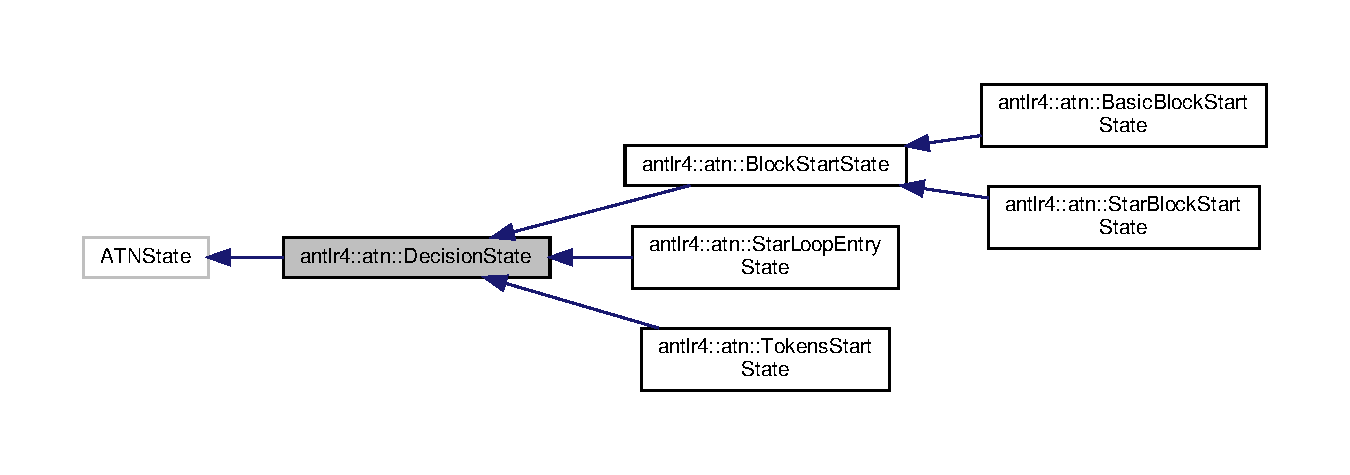
\includegraphics[width=350pt]{classantlr4_1_1atn_1_1DecisionState__inherit__graph}
\end{center}
\end{figure}


Collaboration diagram for antlr4\+:\+:atn\+:\+:Decision\+State\+:
\nopagebreak
\begin{figure}[H]
\begin{center}
\leavevmode
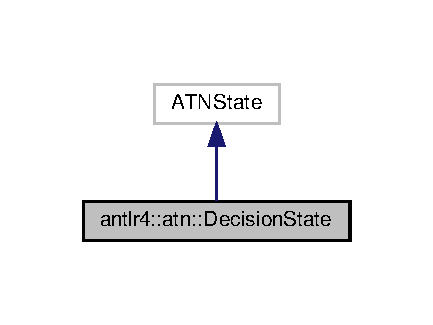
\includegraphics[width=208pt]{classantlr4_1_1atn_1_1DecisionState__coll__graph}
\end{center}
\end{figure}
\subsection*{Public Member Functions}
\begin{DoxyCompactItemize}
\item 
\mbox{\Hypertarget{classantlr4_1_1atn_1_1DecisionState_a30e21564791b80bbe0cd93d4444a29de}\label{classantlr4_1_1atn_1_1DecisionState_a30e21564791b80bbe0cd93d4444a29de}} 
virtual std\+::string {\bfseries to\+String} () const override
\end{DoxyCompactItemize}
\subsection*{Public Attributes}
\begin{DoxyCompactItemize}
\item 
\mbox{\Hypertarget{classantlr4_1_1atn_1_1DecisionState_a6b60a58733e6053e9f35b134883cac68}\label{classantlr4_1_1atn_1_1DecisionState_a6b60a58733e6053e9f35b134883cac68}} 
int {\bfseries decision}
\item 
\mbox{\Hypertarget{classantlr4_1_1atn_1_1DecisionState_ace7d3296421c18e45536e1958a9ee724}\label{classantlr4_1_1atn_1_1DecisionState_ace7d3296421c18e45536e1958a9ee724}} 
bool {\bfseries non\+Greedy}
\end{DoxyCompactItemize}


The documentation for this class was generated from the following files\+:\begin{DoxyCompactItemize}
\item 
atn/Decision\+State.\+h\item 
atn/Decision\+State.\+cpp\end{DoxyCompactItemize}

\hypertarget{classantlr4_1_1DefaultErrorStrategy}{}\section{antlr4\+:\+:Default\+Error\+Strategy Class Reference}
\label{classantlr4_1_1DefaultErrorStrategy}\index{antlr4\+::\+Default\+Error\+Strategy@{antlr4\+::\+Default\+Error\+Strategy}}


{\ttfamily \#include $<$Default\+Error\+Strategy.\+h$>$}



Inheritance diagram for antlr4\+:\+:Default\+Error\+Strategy\+:
\nopagebreak
\begin{figure}[H]
\begin{center}
\leavevmode
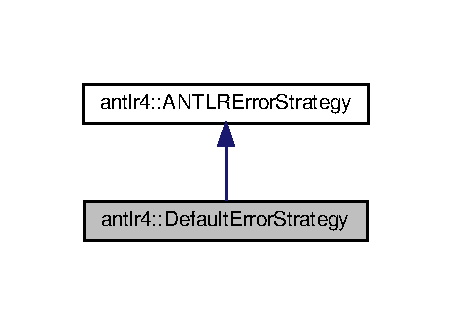
\includegraphics[width=217pt]{classantlr4_1_1DefaultErrorStrategy__inherit__graph}
\end{center}
\end{figure}


Collaboration diagram for antlr4\+:\+:Default\+Error\+Strategy\+:
\nopagebreak
\begin{figure}[H]
\begin{center}
\leavevmode
\includegraphics[width=350pt]{classantlr4_1_1DefaultErrorStrategy__coll__graph}
\end{center}
\end{figure}
\subsection*{Public Member Functions}
\begin{DoxyCompactItemize}
\item 
\mbox{\Hypertarget{classantlr4_1_1DefaultErrorStrategy_ae33bdf3cec035b4232bc7b00cccdb76a}\label{classantlr4_1_1DefaultErrorStrategy_ae33bdf3cec035b4232bc7b00cccdb76a}} 
{\bfseries Default\+Error\+Strategy} (\hyperlink{classantlr4_1_1DefaultErrorStrategy}{Default\+Error\+Strategy} const \&other)=delete
\item 
\mbox{\Hypertarget{classantlr4_1_1DefaultErrorStrategy_ae0a3e0ea5418c980a92a471e26ecfb59}\label{classantlr4_1_1DefaultErrorStrategy_ae0a3e0ea5418c980a92a471e26ecfb59}} 
\hyperlink{classantlr4_1_1DefaultErrorStrategy}{Default\+Error\+Strategy} \& {\bfseries operator=} (\hyperlink{classantlr4_1_1DefaultErrorStrategy}{Default\+Error\+Strategy} const \&other)=delete
\item 
virtual void \hyperlink{classantlr4_1_1DefaultErrorStrategy_a09526cdda0619309a8063dbfe8138c2d}{reset} (\hyperlink{classantlr4_1_1Parser}{Parser} $\ast$recognizer) override
\begin{DoxyCompactList}\small\item\em The default implementation simply calls \begin{DoxySeeAlso}{See also}
\hyperlink{classantlr4_1_1DefaultErrorStrategy_ae04080b08ef36ab9586fe2273ce960f0}{end\+Error\+Condition}


\end{DoxySeeAlso}
to ensure that the handler is not in error recovery mode. \end{DoxyCompactList}\item 
virtual bool \hyperlink{classantlr4_1_1DefaultErrorStrategy_a354b6e4152a68a2b7d9c1357a49ec3cc}{in\+Error\+Recovery\+Mode} (\hyperlink{classantlr4_1_1Parser}{Parser} $\ast$recognizer) override
\item 
virtual void \hyperlink{classantlr4_1_1DefaultErrorStrategy_a9ec4d98c54d479e46909579fb3460300}{report\+Match} (\hyperlink{classantlr4_1_1Parser}{Parser} $\ast$recognizer) override
\begin{DoxyCompactList}\small\item\em The default implementation simply calls \begin{DoxySeeAlso}{See also}
\hyperlink{classantlr4_1_1DefaultErrorStrategy_ae04080b08ef36ab9586fe2273ce960f0}{end\+Error\+Condition}


\end{DoxySeeAlso}
. \end{DoxyCompactList}\end{DoxyCompactItemize}
\subsection*{Protected Member Functions}
\begin{DoxyCompactItemize}
\item 
virtual void \hyperlink{classantlr4_1_1DefaultErrorStrategy_a6408837d5375351acbcd1595c8d5ab79}{begin\+Error\+Condition} (\hyperlink{classantlr4_1_1Parser}{Parser} $\ast$recognizer)
\begin{DoxyCompactList}\small\item\em This method is called to enter error recovery mode when a recognition exception is reported. \end{DoxyCompactList}\item 
virtual void \hyperlink{classantlr4_1_1DefaultErrorStrategy_ae04080b08ef36ab9586fe2273ce960f0}{end\+Error\+Condition} (\hyperlink{classantlr4_1_1Parser}{Parser} $\ast$recognizer)
\begin{DoxyCompactList}\small\item\em This method is called to leave error recovery mode after recovering from a recognition exception. \end{DoxyCompactList}\end{DoxyCompactItemize}
\subsection*{Protected Attributes}
\begin{DoxyCompactItemize}
\item 
bool \hyperlink{classantlr4_1_1DefaultErrorStrategy_a612c641ac64e59200bfeaf1f52b8e31e}{error\+Recovery\+Mode}
\item 
int \hyperlink{classantlr4_1_1DefaultErrorStrategy_ac0c7e89ac7e3c12ca0e44f0d2bda5faa}{last\+Error\+Index}
\item 
\mbox{\Hypertarget{classantlr4_1_1DefaultErrorStrategy_afe3424fbb3b19bca2a9ce4e9ca281d9a}\label{classantlr4_1_1DefaultErrorStrategy_afe3424fbb3b19bca2a9ce4e9ca281d9a}} 
\hyperlink{classantlr4_1_1misc_1_1IntervalSet}{misc\+::\+Interval\+Set} {\bfseries last\+Error\+States}
\end{DoxyCompactItemize}


\subsection{Detailed Description}
This is the default implementation of \hyperlink{classantlr4_1_1ANTLRErrorStrategy}{A\+N\+T\+L\+R\+Error\+Strategy} used for error reporting and recovery in A\+N\+T\+LR parsers. 

\subsection{Member Function Documentation}
\mbox{\Hypertarget{classantlr4_1_1DefaultErrorStrategy_a6408837d5375351acbcd1595c8d5ab79}\label{classantlr4_1_1DefaultErrorStrategy_a6408837d5375351acbcd1595c8d5ab79}} 
\index{antlr4\+::\+Default\+Error\+Strategy@{antlr4\+::\+Default\+Error\+Strategy}!begin\+Error\+Condition@{begin\+Error\+Condition}}
\index{begin\+Error\+Condition@{begin\+Error\+Condition}!antlr4\+::\+Default\+Error\+Strategy@{antlr4\+::\+Default\+Error\+Strategy}}
\subsubsection{\texorpdfstring{begin\+Error\+Condition()}{beginErrorCondition()}}
{\footnotesize\ttfamily void Default\+Error\+Strategy\+::begin\+Error\+Condition (\begin{DoxyParamCaption}\item[{\hyperlink{classantlr4_1_1Parser}{Parser} $\ast$}]{recognizer }\end{DoxyParamCaption})\hspace{0.3cm}{\ttfamily [protected]}, {\ttfamily [virtual]}}



This method is called to enter error recovery mode when a recognition exception is reported. 


\begin{DoxyParams}{Parameters}
{\em recognizer} & the parser instance \\
\hline
\end{DoxyParams}
\mbox{\Hypertarget{classantlr4_1_1DefaultErrorStrategy_ae04080b08ef36ab9586fe2273ce960f0}\label{classantlr4_1_1DefaultErrorStrategy_ae04080b08ef36ab9586fe2273ce960f0}} 
\index{antlr4\+::\+Default\+Error\+Strategy@{antlr4\+::\+Default\+Error\+Strategy}!end\+Error\+Condition@{end\+Error\+Condition}}
\index{end\+Error\+Condition@{end\+Error\+Condition}!antlr4\+::\+Default\+Error\+Strategy@{antlr4\+::\+Default\+Error\+Strategy}}
\subsubsection{\texorpdfstring{end\+Error\+Condition()}{endErrorCondition()}}
{\footnotesize\ttfamily void Default\+Error\+Strategy\+::end\+Error\+Condition (\begin{DoxyParamCaption}\item[{\hyperlink{classantlr4_1_1Parser}{Parser} $\ast$}]{recognizer }\end{DoxyParamCaption})\hspace{0.3cm}{\ttfamily [protected]}, {\ttfamily [virtual]}}



This method is called to leave error recovery mode after recovering from a recognition exception. 


\begin{DoxyParams}{Parameters}
{\em recognizer} & \\
\hline
\end{DoxyParams}
\mbox{\Hypertarget{classantlr4_1_1DefaultErrorStrategy_a354b6e4152a68a2b7d9c1357a49ec3cc}\label{classantlr4_1_1DefaultErrorStrategy_a354b6e4152a68a2b7d9c1357a49ec3cc}} 
\index{antlr4\+::\+Default\+Error\+Strategy@{antlr4\+::\+Default\+Error\+Strategy}!in\+Error\+Recovery\+Mode@{in\+Error\+Recovery\+Mode}}
\index{in\+Error\+Recovery\+Mode@{in\+Error\+Recovery\+Mode}!antlr4\+::\+Default\+Error\+Strategy@{antlr4\+::\+Default\+Error\+Strategy}}
\subsubsection{\texorpdfstring{in\+Error\+Recovery\+Mode()}{inErrorRecoveryMode()}}
{\footnotesize\ttfamily bool Default\+Error\+Strategy\+::in\+Error\+Recovery\+Mode (\begin{DoxyParamCaption}\item[{\hyperlink{classantlr4_1_1Parser}{Parser} $\ast$}]{recognizer }\end{DoxyParamCaption})\hspace{0.3cm}{\ttfamily [override]}, {\ttfamily [virtual]}}





\mbox{\Hypertarget{classantlr4_1_1DefaultErrorStrategy_a9ec4d98c54d479e46909579fb3460300}\label{classantlr4_1_1DefaultErrorStrategy_a9ec4d98c54d479e46909579fb3460300}} 
\index{antlr4\+::\+Default\+Error\+Strategy@{antlr4\+::\+Default\+Error\+Strategy}!report\+Match@{report\+Match}}
\index{report\+Match@{report\+Match}!antlr4\+::\+Default\+Error\+Strategy@{antlr4\+::\+Default\+Error\+Strategy}}
\subsubsection{\texorpdfstring{report\+Match()}{reportMatch()}}
{\footnotesize\ttfamily void Default\+Error\+Strategy\+::report\+Match (\begin{DoxyParamCaption}\item[{\hyperlink{classantlr4_1_1Parser}{Parser} $\ast$}]{recognizer }\end{DoxyParamCaption})\hspace{0.3cm}{\ttfamily [override]}, {\ttfamily [virtual]}}



The default implementation simply calls \begin{DoxySeeAlso}{See also}
\hyperlink{classantlr4_1_1DefaultErrorStrategy_ae04080b08ef36ab9586fe2273ce960f0}{end\+Error\+Condition}


\end{DoxySeeAlso}
. 

\mbox{\Hypertarget{classantlr4_1_1DefaultErrorStrategy_a09526cdda0619309a8063dbfe8138c2d}\label{classantlr4_1_1DefaultErrorStrategy_a09526cdda0619309a8063dbfe8138c2d}} 
\index{antlr4\+::\+Default\+Error\+Strategy@{antlr4\+::\+Default\+Error\+Strategy}!reset@{reset}}
\index{reset@{reset}!antlr4\+::\+Default\+Error\+Strategy@{antlr4\+::\+Default\+Error\+Strategy}}
\subsubsection{\texorpdfstring{reset()}{reset()}}
{\footnotesize\ttfamily void Default\+Error\+Strategy\+::reset (\begin{DoxyParamCaption}\item[{\hyperlink{classantlr4_1_1Parser}{Parser} $\ast$}]{recognizer }\end{DoxyParamCaption})\hspace{0.3cm}{\ttfamily [override]}, {\ttfamily [virtual]}}



The default implementation simply calls \begin{DoxySeeAlso}{See also}
\hyperlink{classantlr4_1_1DefaultErrorStrategy_ae04080b08ef36ab9586fe2273ce960f0}{end\+Error\+Condition}


\end{DoxySeeAlso}
to ensure that the handler is not in error recovery mode. 



\subsection{Member Data Documentation}
\mbox{\Hypertarget{classantlr4_1_1DefaultErrorStrategy_a612c641ac64e59200bfeaf1f52b8e31e}\label{classantlr4_1_1DefaultErrorStrategy_a612c641ac64e59200bfeaf1f52b8e31e}} 
\index{antlr4\+::\+Default\+Error\+Strategy@{antlr4\+::\+Default\+Error\+Strategy}!error\+Recovery\+Mode@{error\+Recovery\+Mode}}
\index{error\+Recovery\+Mode@{error\+Recovery\+Mode}!antlr4\+::\+Default\+Error\+Strategy@{antlr4\+::\+Default\+Error\+Strategy}}
\subsubsection{\texorpdfstring{error\+Recovery\+Mode}{errorRecoveryMode}}
{\footnotesize\ttfamily bool antlr4\+::\+Default\+Error\+Strategy\+::error\+Recovery\+Mode\hspace{0.3cm}{\ttfamily [protected]}}

Indicates whether the error strategy is currently \char`\"{}recovering from an
error\char`\"{}. This is used to suppress reporting multiple error messages while attempting to recover from a detected syntax error.

\begin{DoxySeeAlso}{See also}
\hyperlink{classantlr4_1_1DefaultErrorStrategy_a354b6e4152a68a2b7d9c1357a49ec3cc}{in\+Error\+Recovery\+Mode} 
\end{DoxySeeAlso}
\mbox{\Hypertarget{classantlr4_1_1DefaultErrorStrategy_ac0c7e89ac7e3c12ca0e44f0d2bda5faa}\label{classantlr4_1_1DefaultErrorStrategy_ac0c7e89ac7e3c12ca0e44f0d2bda5faa}} 
\index{antlr4\+::\+Default\+Error\+Strategy@{antlr4\+::\+Default\+Error\+Strategy}!last\+Error\+Index@{last\+Error\+Index}}
\index{last\+Error\+Index@{last\+Error\+Index}!antlr4\+::\+Default\+Error\+Strategy@{antlr4\+::\+Default\+Error\+Strategy}}
\subsubsection{\texorpdfstring{last\+Error\+Index}{lastErrorIndex}}
{\footnotesize\ttfamily int antlr4\+::\+Default\+Error\+Strategy\+::last\+Error\+Index\hspace{0.3cm}{\ttfamily [protected]}}

The index into the input stream where the last error occurred. This is used to prevent infinite loops where an error is found but no token is consumed during recovery...another error is found, ad nauseum. This is a failsafe mechanism to guarantee that at least one token/tree node is consumed for two errors. 

The documentation for this class was generated from the following files\+:\begin{DoxyCompactItemize}
\item 
Default\+Error\+Strategy.\+h\item 
Default\+Error\+Strategy.\+cpp\end{DoxyCompactItemize}

\hypertarget{classantlr4_1_1dfa_1_1DFA}{}\section{antlr4\+:\+:dfa\+:\+:D\+FA Class Reference}
\label{classantlr4_1_1dfa_1_1DFA}\index{antlr4\+::dfa\+::\+D\+FA@{antlr4\+::dfa\+::\+D\+FA}}


Collaboration diagram for antlr4\+:\+:dfa\+:\+:D\+FA\+:
\nopagebreak
\begin{figure}[H]
\begin{center}
\leavevmode
\includegraphics[width=208pt]{classantlr4_1_1dfa_1_1DFA__coll__graph}
\end{center}
\end{figure}
\subsection*{Public Member Functions}
\begin{DoxyCompactItemize}
\item 
\mbox{\Hypertarget{classantlr4_1_1dfa_1_1DFA_a96e1072f740839921fb72b3b9e9db330}\label{classantlr4_1_1dfa_1_1DFA_a96e1072f740839921fb72b3b9e9db330}} 
{\bfseries D\+FA} (\hyperlink{classantlr4_1_1atn_1_1DecisionState}{atn\+::\+Decision\+State} $\ast$\hyperlink{classantlr4_1_1dfa_1_1DFA_a83d51316351c6939e7d249dc20b5c9c8}{atn\+Start\+State})
\item 
\mbox{\Hypertarget{classantlr4_1_1dfa_1_1DFA_a2597bff5bd2fea39907a0dfb02f9f8ac}\label{classantlr4_1_1dfa_1_1DFA_a2597bff5bd2fea39907a0dfb02f9f8ac}} 
{\bfseries D\+FA} (\hyperlink{classantlr4_1_1atn_1_1DecisionState}{atn\+::\+Decision\+State} $\ast$\hyperlink{classantlr4_1_1dfa_1_1DFA_a83d51316351c6939e7d249dc20b5c9c8}{atn\+Start\+State}, size\+\_\+t decision)
\item 
\mbox{\Hypertarget{classantlr4_1_1dfa_1_1DFA_a25516f53c648275fb491921d7f421260}\label{classantlr4_1_1dfa_1_1DFA_a25516f53c648275fb491921d7f421260}} 
{\bfseries D\+FA} (const \hyperlink{classantlr4_1_1dfa_1_1DFA}{D\+FA} \&other)=delete
\item 
\mbox{\Hypertarget{classantlr4_1_1dfa_1_1DFA_a4ada17f3f123b29d5bd965909bac28ee}\label{classantlr4_1_1dfa_1_1DFA_a4ada17f3f123b29d5bd965909bac28ee}} 
{\bfseries D\+FA} (\hyperlink{classantlr4_1_1dfa_1_1DFA}{D\+FA} \&\&other)
\item 
bool \hyperlink{classantlr4_1_1dfa_1_1DFA_a16f04e1d91f059b882505aff2174a1e1}{is\+Precedence\+Dfa} () const
\item 
D\+F\+A\+State $\ast$ \hyperlink{classantlr4_1_1dfa_1_1DFA_a6e0d2aca83d6cb0d155d971594c8dc7f}{get\+Precedence\+Start\+State} (int precedence) const
\item 
void \hyperlink{classantlr4_1_1dfa_1_1DFA_a0283251c54b224124da6fc0600717617}{set\+Precedence\+Start\+State} (int precedence, D\+F\+A\+State $\ast$start\+State, \hyperlink{classantlrcpp_1_1SingleWriteMultipleReadLock}{antlrcpp\+::\+Single\+Write\+Multiple\+Read\+Lock} \&lock)
\item 
\mbox{\Hypertarget{classantlr4_1_1dfa_1_1DFA_afe9610a3706058c0d5d1e61f386ccd29}\label{classantlr4_1_1dfa_1_1DFA_afe9610a3706058c0d5d1e61f386ccd29}} 
virtual std\+::vector$<$ D\+F\+A\+State $\ast$ $>$ \hyperlink{classantlr4_1_1dfa_1_1DFA_afe9610a3706058c0d5d1e61f386ccd29}{get\+States} () const
\begin{DoxyCompactList}\small\item\em Return a list of all states in this \hyperlink{classantlr4_1_1dfa_1_1DFA}{D\+FA}, ordered by state number. \end{DoxyCompactList}\item 
virtual std\+::string \hyperlink{classantlr4_1_1dfa_1_1DFA_adae4f569d3075101ae3571fe67748b56}{to\+String} (const std\+::vector$<$ std\+::string $>$ \&token\+Names)
\item 
\mbox{\Hypertarget{classantlr4_1_1dfa_1_1DFA_a47082a53818c84418ed873c64b7d2951}\label{classantlr4_1_1dfa_1_1DFA_a47082a53818c84418ed873c64b7d2951}} 
std\+::string {\bfseries to\+String} (const Vocabulary \&vocabulary) const
\item 
\mbox{\Hypertarget{classantlr4_1_1dfa_1_1DFA_a17f180730ab4ac077e4811665ec1e0e0}\label{classantlr4_1_1dfa_1_1DFA_a17f180730ab4ac077e4811665ec1e0e0}} 
virtual std\+::string {\bfseries to\+Lexer\+String} ()
\end{DoxyCompactItemize}
\subsection*{Public Attributes}
\begin{DoxyCompactItemize}
\item 
\hyperlink{classantlr4_1_1atn_1_1DecisionState}{atn\+::\+Decision\+State} $\ast$ \hyperlink{classantlr4_1_1dfa_1_1DFA_a83d51316351c6939e7d249dc20b5c9c8}{atn\+Start\+State}
\begin{DoxyCompactList}\small\item\em From which A\+TN state did we create this \hyperlink{classantlr4_1_1dfa_1_1DFA}{D\+FA}? \end{DoxyCompactList}\item 
\mbox{\Hypertarget{classantlr4_1_1dfa_1_1DFA_a287490e94942bf6355b041e13b4fcc1c}\label{classantlr4_1_1dfa_1_1DFA_a287490e94942bf6355b041e13b4fcc1c}} 
std\+::unordered\+\_\+set$<$ D\+F\+A\+State $\ast$, D\+F\+A\+State\+::\+Hasher, D\+F\+A\+State\+::\+Comparer $>$ {\bfseries states}
\item 
\mbox{\Hypertarget{classantlr4_1_1dfa_1_1DFA_a42e1ce8d87cbfb6156a6bff4fd86ed32}\label{classantlr4_1_1dfa_1_1DFA_a42e1ce8d87cbfb6156a6bff4fd86ed32}} 
D\+F\+A\+State $\ast$ {\bfseries s0}
\item 
\mbox{\Hypertarget{classantlr4_1_1dfa_1_1DFA_afaf75312829a34946e8e69b07748a230}\label{classantlr4_1_1dfa_1_1DFA_afaf75312829a34946e8e69b07748a230}} 
size\+\_\+t {\bfseries decision}
\end{DoxyCompactItemize}


\subsection{Member Function Documentation}
\mbox{\Hypertarget{classantlr4_1_1dfa_1_1DFA_a6e0d2aca83d6cb0d155d971594c8dc7f}\label{classantlr4_1_1dfa_1_1DFA_a6e0d2aca83d6cb0d155d971594c8dc7f}} 
\index{antlr4\+::dfa\+::\+D\+FA@{antlr4\+::dfa\+::\+D\+FA}!get\+Precedence\+Start\+State@{get\+Precedence\+Start\+State}}
\index{get\+Precedence\+Start\+State@{get\+Precedence\+Start\+State}!antlr4\+::dfa\+::\+D\+FA@{antlr4\+::dfa\+::\+D\+FA}}
\subsubsection{\texorpdfstring{get\+Precedence\+Start\+State()}{getPrecedenceStartState()}}
{\footnotesize\ttfamily D\+F\+A\+State $\ast$ D\+F\+A\+::get\+Precedence\+Start\+State (\begin{DoxyParamCaption}\item[{int}]{precedence }\end{DoxyParamCaption}) const}

Get the start state for a specific precedence value.


\begin{DoxyParams}{Parameters}
{\em precedence} & The current precedence. \\
\hline
\end{DoxyParams}
\begin{DoxyReturn}{Returns}
The start state corresponding to the specified precedence, or 
\begin{DoxyCode}
null 
\end{DoxyCode}
 if no start state exists for the specified precedence.
\end{DoxyReturn}

\begin{DoxyExceptions}{Exceptions}
{\em \hyperlink{classantlr4_1_1IllegalStateException}{Illegal\+State\+Exception}} & if this is not a precedence \hyperlink{classantlr4_1_1dfa_1_1DFA}{D\+FA}. \\
\hline
\end{DoxyExceptions}
\begin{DoxySeeAlso}{See also}
\hyperlink{classantlr4_1_1dfa_1_1DFA_a16f04e1d91f059b882505aff2174a1e1}{is\+Precedence\+Dfa()} 
\end{DoxySeeAlso}
\mbox{\Hypertarget{classantlr4_1_1dfa_1_1DFA_a16f04e1d91f059b882505aff2174a1e1}\label{classantlr4_1_1dfa_1_1DFA_a16f04e1d91f059b882505aff2174a1e1}} 
\index{antlr4\+::dfa\+::\+D\+FA@{antlr4\+::dfa\+::\+D\+FA}!is\+Precedence\+Dfa@{is\+Precedence\+Dfa}}
\index{is\+Precedence\+Dfa@{is\+Precedence\+Dfa}!antlr4\+::dfa\+::\+D\+FA@{antlr4\+::dfa\+::\+D\+FA}}
\subsubsection{\texorpdfstring{is\+Precedence\+Dfa()}{isPrecedenceDfa()}}
{\footnotesize\ttfamily bool D\+F\+A\+::is\+Precedence\+Dfa (\begin{DoxyParamCaption}{ }\end{DoxyParamCaption}) const}

Gets whether this \hyperlink{classantlr4_1_1dfa_1_1DFA}{D\+FA} is a precedence \hyperlink{classantlr4_1_1dfa_1_1DFA}{D\+FA}. Precedence D\+F\+As use a special start state \hyperlink{}{s0} which is not stored in \hyperlink{}{states}. The \hyperlink{}{D\+F\+A\+State\#edges} array for this start state contains outgoing edges supplying individual start states corresponding to specific precedence values.

\begin{DoxyReturn}{Returns}

\begin{DoxyCode}
\textcolor{keyword}{true} 
\end{DoxyCode}
 if this is a precedence \hyperlink{classantlr4_1_1dfa_1_1DFA}{D\+FA}; otherwise, 
\begin{DoxyCode}
\textcolor{keyword}{false} 
\end{DoxyCode}
 . 
\end{DoxyReturn}
\begin{DoxySeeAlso}{See also}
Parser\+::get\+Precedence() 
\end{DoxySeeAlso}
\mbox{\Hypertarget{classantlr4_1_1dfa_1_1DFA_a0283251c54b224124da6fc0600717617}\label{classantlr4_1_1dfa_1_1DFA_a0283251c54b224124da6fc0600717617}} 
\index{antlr4\+::dfa\+::\+D\+FA@{antlr4\+::dfa\+::\+D\+FA}!set\+Precedence\+Start\+State@{set\+Precedence\+Start\+State}}
\index{set\+Precedence\+Start\+State@{set\+Precedence\+Start\+State}!antlr4\+::dfa\+::\+D\+FA@{antlr4\+::dfa\+::\+D\+FA}}
\subsubsection{\texorpdfstring{set\+Precedence\+Start\+State()}{setPrecedenceStartState()}}
{\footnotesize\ttfamily void D\+F\+A\+::set\+Precedence\+Start\+State (\begin{DoxyParamCaption}\item[{int}]{precedence,  }\item[{D\+F\+A\+State $\ast$}]{start\+State,  }\item[{\hyperlink{classantlrcpp_1_1SingleWriteMultipleReadLock}{antlrcpp\+::\+Single\+Write\+Multiple\+Read\+Lock} \&}]{lock }\end{DoxyParamCaption})}

Set the start state for a specific precedence value.


\begin{DoxyParams}{Parameters}
{\em precedence} & The current precedence. \\
\hline
{\em start\+State} & The start state corresponding to the specified precedence.\\
\hline
\end{DoxyParams}

\begin{DoxyExceptions}{Exceptions}
{\em \hyperlink{classantlr4_1_1IllegalStateException}{Illegal\+State\+Exception}} & if this is not a precedence \hyperlink{classantlr4_1_1dfa_1_1DFA}{D\+FA}. \\
\hline
\end{DoxyExceptions}
\begin{DoxySeeAlso}{See also}
\hyperlink{classantlr4_1_1dfa_1_1DFA_a16f04e1d91f059b882505aff2174a1e1}{is\+Precedence\+Dfa()} 
\end{DoxySeeAlso}
\mbox{\Hypertarget{classantlr4_1_1dfa_1_1DFA_adae4f569d3075101ae3571fe67748b56}\label{classantlr4_1_1dfa_1_1DFA_adae4f569d3075101ae3571fe67748b56}} 
\index{antlr4\+::dfa\+::\+D\+FA@{antlr4\+::dfa\+::\+D\+FA}!to\+String@{to\+String}}
\index{to\+String@{to\+String}!antlr4\+::dfa\+::\+D\+FA@{antlr4\+::dfa\+::\+D\+FA}}
\subsubsection{\texorpdfstring{to\+String()}{toString()}}
{\footnotesize\ttfamily std\+::string D\+F\+A\+::to\+String (\begin{DoxyParamCaption}\item[{const std\+::vector$<$ std\+::string $>$ \&}]{token\+Names }\end{DoxyParamCaption})\hspace{0.3cm}{\ttfamily [virtual]}}

\begin{DoxyRefDesc}{Deprecated}
\item[\hyperlink{deprecated__deprecated000007}{Deprecated}]Use \hyperlink{}{to\+String(\+Vocabulary)} instead. \end{DoxyRefDesc}


\subsection{Member Data Documentation}
\mbox{\Hypertarget{classantlr4_1_1dfa_1_1DFA_a83d51316351c6939e7d249dc20b5c9c8}\label{classantlr4_1_1dfa_1_1DFA_a83d51316351c6939e7d249dc20b5c9c8}} 
\index{antlr4\+::dfa\+::\+D\+FA@{antlr4\+::dfa\+::\+D\+FA}!atn\+Start\+State@{atn\+Start\+State}}
\index{atn\+Start\+State@{atn\+Start\+State}!antlr4\+::dfa\+::\+D\+FA@{antlr4\+::dfa\+::\+D\+FA}}
\subsubsection{\texorpdfstring{atn\+Start\+State}{atnStartState}}
{\footnotesize\ttfamily \hyperlink{classantlr4_1_1atn_1_1DecisionState}{atn\+::\+Decision\+State}$\ast$ antlr4\+::dfa\+::\+D\+F\+A\+::atn\+Start\+State}



From which A\+TN state did we create this \hyperlink{classantlr4_1_1dfa_1_1DFA}{D\+FA}? 

A set of all \hyperlink{classantlr4_1_1dfa_1_1DFA}{D\+FA} states. Use a map so we can get old state back. Set only allows you to see if it\textquotesingle{}s there. 

The documentation for this class was generated from the following files\+:\begin{DoxyCompactItemize}
\item 
dfa/D\+F\+A.\+h\item 
dfa/D\+F\+A.\+cpp\end{DoxyCompactItemize}

\hypertarget{classantlr4_1_1dfa_1_1DFASerializer}{}\section{antlr4\+:\+:dfa\+:\+:D\+F\+A\+Serializer Class Reference}
\label{classantlr4_1_1dfa_1_1DFASerializer}\index{antlr4\+::dfa\+::\+D\+F\+A\+Serializer@{antlr4\+::dfa\+::\+D\+F\+A\+Serializer}}


A \hyperlink{classantlr4_1_1dfa_1_1DFA}{D\+FA} walker that knows how to dump them to serialized strings.  




{\ttfamily \#include $<$D\+F\+A\+Serializer.\+h$>$}



Inheritance diagram for antlr4\+:\+:dfa\+:\+:D\+F\+A\+Serializer\+:
\nopagebreak
\begin{figure}[H]
\begin{center}
\leavevmode
\includegraphics[width=231pt]{classantlr4_1_1dfa_1_1DFASerializer__inherit__graph}
\end{center}
\end{figure}
\subsection*{Public Member Functions}
\begin{DoxyCompactItemize}
\item 
\mbox{\Hypertarget{classantlr4_1_1dfa_1_1DFASerializer_a4ddb2f4485acb92f0d7c788cc6e3550c}\label{classantlr4_1_1dfa_1_1DFASerializer_a4ddb2f4485acb92f0d7c788cc6e3550c}} 
{\bfseries D\+F\+A\+Serializer} (const \hyperlink{classantlr4_1_1dfa_1_1DFA}{D\+FA} $\ast$dfa, const std\+::vector$<$ std\+::string $>$ \&tnames)
\item 
\mbox{\Hypertarget{classantlr4_1_1dfa_1_1DFASerializer_a53b2f8347bf1964c90d0085ae16b0777}\label{classantlr4_1_1dfa_1_1DFASerializer_a53b2f8347bf1964c90d0085ae16b0777}} 
{\bfseries D\+F\+A\+Serializer} (const \hyperlink{classantlr4_1_1dfa_1_1DFA}{D\+FA} $\ast$dfa, const Vocabulary \&vocabulary)
\item 
\mbox{\Hypertarget{classantlr4_1_1dfa_1_1DFASerializer_a3a459289bc5dac02365e5474a51ade1d}\label{classantlr4_1_1dfa_1_1DFASerializer_a3a459289bc5dac02365e5474a51ade1d}} 
virtual std\+::string {\bfseries to\+String} () const
\end{DoxyCompactItemize}
\subsection*{Protected Member Functions}
\begin{DoxyCompactItemize}
\item 
\mbox{\Hypertarget{classantlr4_1_1dfa_1_1DFASerializer_a93719dde2778b820567b40726e896610}\label{classantlr4_1_1dfa_1_1DFASerializer_a93719dde2778b820567b40726e896610}} 
virtual std\+::string {\bfseries get\+Edge\+Label} (size\+\_\+t i) const
\item 
\mbox{\Hypertarget{classantlr4_1_1dfa_1_1DFASerializer_acc1d210c8d845dbc2ecf21c497ecbfaa}\label{classantlr4_1_1dfa_1_1DFASerializer_acc1d210c8d845dbc2ecf21c497ecbfaa}} 
virtual std\+::string {\bfseries get\+State\+String} (D\+F\+A\+State $\ast$s) const
\end{DoxyCompactItemize}


\subsection{Detailed Description}
A \hyperlink{classantlr4_1_1dfa_1_1DFA}{D\+FA} walker that knows how to dump them to serialized strings. 

The documentation for this class was generated from the following files\+:\begin{DoxyCompactItemize}
\item 
dfa/D\+F\+A\+Serializer.\+h\item 
dfa/D\+F\+A\+Serializer.\+cpp\end{DoxyCompactItemize}

\hypertarget{classantlr4_1_1atn_1_1EmptyPredictionContext}{}\section{antlr4\+:\+:atn\+:\+:Empty\+Prediction\+Context Class Reference}
\label{classantlr4_1_1atn_1_1EmptyPredictionContext}\index{antlr4\+::atn\+::\+Empty\+Prediction\+Context@{antlr4\+::atn\+::\+Empty\+Prediction\+Context}}


Inheritance diagram for antlr4\+:\+:atn\+:\+:Empty\+Prediction\+Context\+:
\nopagebreak
\begin{figure}[H]
\begin{center}
\leavevmode
\includegraphics[width=230pt]{classantlr4_1_1atn_1_1EmptyPredictionContext__inherit__graph}
\end{center}
\end{figure}


Collaboration diagram for antlr4\+:\+:atn\+:\+:Empty\+Prediction\+Context\+:
\nopagebreak
\begin{figure}[H]
\begin{center}
\leavevmode
\includegraphics[width=230pt]{classantlr4_1_1atn_1_1EmptyPredictionContext__coll__graph}
\end{center}
\end{figure}
\subsection*{Public Member Functions}
\begin{DoxyCompactItemize}
\item 
\mbox{\Hypertarget{classantlr4_1_1atn_1_1EmptyPredictionContext_a0216ff499b88ca1443ae9e720541b5ce}\label{classantlr4_1_1atn_1_1EmptyPredictionContext_a0216ff499b88ca1443ae9e720541b5ce}} 
virtual bool \hyperlink{classantlr4_1_1atn_1_1EmptyPredictionContext_a0216ff499b88ca1443ae9e720541b5ce}{is\+Empty} () const override
\begin{DoxyCompactList}\small\item\em This means only the E\+M\+P\+TY (wildcard? not sure) context is in set. \end{DoxyCompactList}\item 
\mbox{\Hypertarget{classantlr4_1_1atn_1_1EmptyPredictionContext_a92d4e1c48bc9daf37cec387a06fc6fad}\label{classantlr4_1_1atn_1_1EmptyPredictionContext_a92d4e1c48bc9daf37cec387a06fc6fad}} 
virtual size\+\_\+t {\bfseries size} () const override
\item 
\mbox{\Hypertarget{classantlr4_1_1atn_1_1EmptyPredictionContext_acd1aaea5711a69c01f23942a78e4678e}\label{classantlr4_1_1atn_1_1EmptyPredictionContext_acd1aaea5711a69c01f23942a78e4678e}} 
virtual Ref$<$ \hyperlink{classantlr4_1_1atn_1_1PredictionContext}{Prediction\+Context} $>$ {\bfseries get\+Parent} (size\+\_\+t index) const override
\item 
\mbox{\Hypertarget{classantlr4_1_1atn_1_1EmptyPredictionContext_a50f13a4b417ac47340985f3212fd81f1}\label{classantlr4_1_1atn_1_1EmptyPredictionContext_a50f13a4b417ac47340985f3212fd81f1}} 
virtual size\+\_\+t {\bfseries get\+Return\+State} (size\+\_\+t index) const override
\item 
\mbox{\Hypertarget{classantlr4_1_1atn_1_1EmptyPredictionContext_ad1e91bf65a589ebdfcefb9d719b3f991}\label{classantlr4_1_1atn_1_1EmptyPredictionContext_ad1e91bf65a589ebdfcefb9d719b3f991}} 
virtual std\+::string {\bfseries to\+String} () const override
\item 
\mbox{\Hypertarget{classantlr4_1_1atn_1_1EmptyPredictionContext_a05692e3c3260fa7669c27b1cc531b780}\label{classantlr4_1_1atn_1_1EmptyPredictionContext_a05692e3c3260fa7669c27b1cc531b780}} 
virtual bool {\bfseries operator==} (const \hyperlink{classantlr4_1_1atn_1_1PredictionContext}{Prediction\+Context} \&o) const override
\end{DoxyCompactItemize}
\subsection*{Additional Inherited Members}


The documentation for this class was generated from the following files\+:\begin{DoxyCompactItemize}
\item 
atn/Empty\+Prediction\+Context.\+h\item 
atn/Empty\+Prediction\+Context.\+cpp\end{DoxyCompactItemize}

\hypertarget{classantlr4_1_1EmptyStackException}{}\section{antlr4\+:\+:Empty\+Stack\+Exception Class Reference}
\label{classantlr4_1_1EmptyStackException}\index{antlr4\+::\+Empty\+Stack\+Exception@{antlr4\+::\+Empty\+Stack\+Exception}}


Inheritance diagram for antlr4\+:\+:Empty\+Stack\+Exception\+:
\nopagebreak
\begin{figure}[H]
\begin{center}
\leavevmode
\includegraphics[width=224pt]{classantlr4_1_1EmptyStackException__inherit__graph}
\end{center}
\end{figure}


Collaboration diagram for antlr4\+:\+:Empty\+Stack\+Exception\+:
\nopagebreak
\begin{figure}[H]
\begin{center}
\leavevmode
\includegraphics[width=224pt]{classantlr4_1_1EmptyStackException__coll__graph}
\end{center}
\end{figure}
\subsection*{Public Member Functions}
\begin{DoxyCompactItemize}
\item 
\mbox{\Hypertarget{classantlr4_1_1EmptyStackException_a0d72af7b155cf625bb078211df68f3f1}\label{classantlr4_1_1EmptyStackException_a0d72af7b155cf625bb078211df68f3f1}} 
{\bfseries Empty\+Stack\+Exception} (const std\+::string \&msg=\char`\"{}\char`\"{})
\item 
\mbox{\Hypertarget{classantlr4_1_1EmptyStackException_a46c40463aaa90db612bdbc8cc4f8290b}\label{classantlr4_1_1EmptyStackException_a46c40463aaa90db612bdbc8cc4f8290b}} 
{\bfseries Empty\+Stack\+Exception} (\hyperlink{classantlr4_1_1EmptyStackException}{Empty\+Stack\+Exception} const \&)=default
\item 
\mbox{\Hypertarget{classantlr4_1_1EmptyStackException_abb155a661cf8cb57fdb7dc66743acf3c}\label{classantlr4_1_1EmptyStackException_abb155a661cf8cb57fdb7dc66743acf3c}} 
\hyperlink{classantlr4_1_1EmptyStackException}{Empty\+Stack\+Exception} \& {\bfseries operator=} (\hyperlink{classantlr4_1_1EmptyStackException}{Empty\+Stack\+Exception} const \&)=default
\end{DoxyCompactItemize}


The documentation for this class was generated from the following files\+:\begin{DoxyCompactItemize}
\item 
Exceptions.\+h\item 
Exceptions.\+cpp\end{DoxyCompactItemize}

\hypertarget{classantlr4_1_1atn_1_1EpsilonTransition}{}\section{antlr4\+:\+:atn\+:\+:Epsilon\+Transition Class Reference}
\label{classantlr4_1_1atn_1_1EpsilonTransition}\index{antlr4\+::atn\+::\+Epsilon\+Transition@{antlr4\+::atn\+::\+Epsilon\+Transition}}


Inheritance diagram for antlr4\+:\+:atn\+:\+:Epsilon\+Transition\+:
\nopagebreak
\begin{figure}[H]
\begin{center}
\leavevmode
\includegraphics[width=221pt]{classantlr4_1_1atn_1_1EpsilonTransition__inherit__graph}
\end{center}
\end{figure}


Collaboration diagram for antlr4\+:\+:atn\+:\+:Epsilon\+Transition\+:
\nopagebreak
\begin{figure}[H]
\begin{center}
\leavevmode
\includegraphics[width=221pt]{classantlr4_1_1atn_1_1EpsilonTransition__coll__graph}
\end{center}
\end{figure}
\subsection*{Public Member Functions}
\begin{DoxyCompactItemize}
\item 
\mbox{\Hypertarget{classantlr4_1_1atn_1_1EpsilonTransition_af9acaefc6f86484a05ffe9f6ffc38ae9}\label{classantlr4_1_1atn_1_1EpsilonTransition_af9acaefc6f86484a05ffe9f6ffc38ae9}} 
{\bfseries Epsilon\+Transition} (A\+T\+N\+State $\ast$\hyperlink{classantlr4_1_1atn_1_1Transition_aaaed7f4ddda71e156b36de33e88f66a7}{target})
\item 
\mbox{\Hypertarget{classantlr4_1_1atn_1_1EpsilonTransition_a89f91655dacff645efa57b23c940bb71}\label{classantlr4_1_1atn_1_1EpsilonTransition_a89f91655dacff645efa57b23c940bb71}} 
{\bfseries Epsilon\+Transition} (A\+T\+N\+State $\ast$\hyperlink{classantlr4_1_1atn_1_1Transition_aaaed7f4ddda71e156b36de33e88f66a7}{target}, size\+\_\+t \hyperlink{classantlr4_1_1atn_1_1EpsilonTransition_adb67e8063ffad68fe759b105547f38c7}{outermost\+Precedence\+Return})
\item 
size\+\_\+t \hyperlink{classantlr4_1_1atn_1_1EpsilonTransition_adb67e8063ffad68fe759b105547f38c7}{outermost\+Precedence\+Return} ()
\item 
\mbox{\Hypertarget{classantlr4_1_1atn_1_1EpsilonTransition_a7a38bb719f9384e33ddb4414795de299}\label{classantlr4_1_1atn_1_1EpsilonTransition_a7a38bb719f9384e33ddb4414795de299}} 
virtual Serialization\+Type {\bfseries get\+Serialization\+Type} () const override
\item 
virtual bool \hyperlink{classantlr4_1_1atn_1_1EpsilonTransition_aa2ed63d1d7605293c69cd812c6e374ec}{is\+Epsilon} () const override
\item 
\mbox{\Hypertarget{classantlr4_1_1atn_1_1EpsilonTransition_a3b259559117c7bd3de00af88f58ca4ba}\label{classantlr4_1_1atn_1_1EpsilonTransition_a3b259559117c7bd3de00af88f58ca4ba}} 
virtual bool {\bfseries matches} (size\+\_\+t symbol, size\+\_\+t min\+Vocab\+Symbol, size\+\_\+t max\+Vocab\+Symbol) const override
\item 
\mbox{\Hypertarget{classantlr4_1_1atn_1_1EpsilonTransition_ad93842a60a917fe5dc199c390a2a2c0c}\label{classantlr4_1_1atn_1_1EpsilonTransition_ad93842a60a917fe5dc199c390a2a2c0c}} 
virtual std\+::string {\bfseries to\+String} () const override
\end{DoxyCompactItemize}
\subsection*{Additional Inherited Members}


\subsection{Member Function Documentation}
\mbox{\Hypertarget{classantlr4_1_1atn_1_1EpsilonTransition_aa2ed63d1d7605293c69cd812c6e374ec}\label{classantlr4_1_1atn_1_1EpsilonTransition_aa2ed63d1d7605293c69cd812c6e374ec}} 
\index{antlr4\+::atn\+::\+Epsilon\+Transition@{antlr4\+::atn\+::\+Epsilon\+Transition}!is\+Epsilon@{is\+Epsilon}}
\index{is\+Epsilon@{is\+Epsilon}!antlr4\+::atn\+::\+Epsilon\+Transition@{antlr4\+::atn\+::\+Epsilon\+Transition}}
\subsubsection{\texorpdfstring{is\+Epsilon()}{isEpsilon()}}
{\footnotesize\ttfamily bool Epsilon\+Transition\+::is\+Epsilon (\begin{DoxyParamCaption}{ }\end{DoxyParamCaption}) const\hspace{0.3cm}{\ttfamily [override]}, {\ttfamily [virtual]}}

Determines if the transition is an \char`\"{}epsilon\char`\"{} transition.

The default implementation returns
\begin{DoxyCode}
\textcolor{keyword}{false} 
\end{DoxyCode}
 .

\begin{DoxyReturn}{Returns}

\begin{DoxyCode}
\textcolor{keyword}{true} 
\end{DoxyCode}
 if traversing this transition in the A\+TN does not consume an input symbol; otherwise,
\begin{DoxyCode}
\textcolor{keyword}{false} 
\end{DoxyCode}
 if traversing this transition consumes (matches) an input symbol. 
\end{DoxyReturn}


Reimplemented from \hyperlink{classantlr4_1_1atn_1_1Transition_a8e712c7a46586d73c054c56f481b1be7}{antlr4\+::atn\+::\+Transition}.

\mbox{\Hypertarget{classantlr4_1_1atn_1_1EpsilonTransition_adb67e8063ffad68fe759b105547f38c7}\label{classantlr4_1_1atn_1_1EpsilonTransition_adb67e8063ffad68fe759b105547f38c7}} 
\index{antlr4\+::atn\+::\+Epsilon\+Transition@{antlr4\+::atn\+::\+Epsilon\+Transition}!outermost\+Precedence\+Return@{outermost\+Precedence\+Return}}
\index{outermost\+Precedence\+Return@{outermost\+Precedence\+Return}!antlr4\+::atn\+::\+Epsilon\+Transition@{antlr4\+::atn\+::\+Epsilon\+Transition}}
\subsubsection{\texorpdfstring{outermost\+Precedence\+Return()}{outermostPrecedenceReturn()}}
{\footnotesize\ttfamily size\+\_\+t Epsilon\+Transition\+::outermost\+Precedence\+Return (\begin{DoxyParamCaption}{ }\end{DoxyParamCaption})}

\begin{DoxyReturn}{Returns}
the rule index of a precedence rule for which this transition is returning from, where the precedence value is 0; otherwise, I\+N\+V\+A\+L\+I\+D\+\_\+\+I\+N\+D\+EX.
\end{DoxyReturn}
\begin{DoxySeeAlso}{See also}
A\+T\+N\+Config\+::is\+Precedence\+Filter\+Suppressed() 

Parser\+A\+T\+N\+Simulator\+::apply\+Precedence\+Filter(\+A\+T\+N\+Config\+Set) 
\end{DoxySeeAlso}
\begin{DoxySince}{Since}
4.\+4.\+1 
\end{DoxySince}


The documentation for this class was generated from the following files\+:\begin{DoxyCompactItemize}
\item 
atn/Epsilon\+Transition.\+h\item 
atn/Epsilon\+Transition.\+cpp\end{DoxyCompactItemize}

\hypertarget{classantlr4_1_1tree_1_1ErrorNode}{}\section{antlr4\+:\+:tree\+:\+:Error\+Node Class Reference}
\label{classantlr4_1_1tree_1_1ErrorNode}\index{antlr4\+::tree\+::\+Error\+Node@{antlr4\+::tree\+::\+Error\+Node}}


Inheritance diagram for antlr4\+:\+:tree\+:\+:Error\+Node\+:
\nopagebreak
\begin{figure}[H]
\begin{center}
\leavevmode
\includegraphics[width=212pt]{classantlr4_1_1tree_1_1ErrorNode__inherit__graph}
\end{center}
\end{figure}


Collaboration diagram for antlr4\+:\+:tree\+:\+:Error\+Node\+:
\nopagebreak
\begin{figure}[H]
\begin{center}
\leavevmode
\includegraphics[width=251pt]{classantlr4_1_1tree_1_1ErrorNode__coll__graph}
\end{center}
\end{figure}
\subsection*{Additional Inherited Members}


The documentation for this class was generated from the following files\+:\begin{DoxyCompactItemize}
\item 
tree/Error\+Node.\+h\item 
tree/Error\+Node.\+cpp\end{DoxyCompactItemize}

\hypertarget{classantlr4_1_1tree_1_1ErrorNodeImpl}{}\section{antlr4\+:\+:tree\+:\+:Error\+Node\+Impl Class Reference}
\label{classantlr4_1_1tree_1_1ErrorNodeImpl}\index{antlr4\+::tree\+::\+Error\+Node\+Impl@{antlr4\+::tree\+::\+Error\+Node\+Impl}}


Represents a token that was consumed during resynchronization rather than during a valid match operation. For example, we will create this kind of a node during single token insertion and deletion as well as during \char`\"{}consume until error recovery set\char`\"{} upon no viable alternative exceptions.  




{\ttfamily \#include $<$Error\+Node\+Impl.\+h$>$}



Inheritance diagram for antlr4\+:\+:tree\+:\+:Error\+Node\+Impl\+:
\nopagebreak
\begin{figure}[H]
\begin{center}
\leavevmode
\includegraphics[width=350pt]{classantlr4_1_1tree_1_1ErrorNodeImpl__inherit__graph}
\end{center}
\end{figure}


Collaboration diagram for antlr4\+:\+:tree\+:\+:Error\+Node\+Impl\+:
\nopagebreak
\begin{figure}[H]
\begin{center}
\leavevmode
\includegraphics[width=350pt]{classantlr4_1_1tree_1_1ErrorNodeImpl__coll__graph}
\end{center}
\end{figure}
\subsection*{Public Member Functions}
\begin{DoxyCompactItemize}
\item 
\mbox{\Hypertarget{classantlr4_1_1tree_1_1ErrorNodeImpl_a62a01a09215038907392f3c861ed0d2e}\label{classantlr4_1_1tree_1_1ErrorNodeImpl_a62a01a09215038907392f3c861ed0d2e}} 
{\bfseries Error\+Node\+Impl} (\hyperlink{classantlr4_1_1Token}{Token} $\ast$token)
\item 
\mbox{\Hypertarget{classantlr4_1_1tree_1_1ErrorNodeImpl_a746a33c109fcce3bbe3e40aab2cdb06b}\label{classantlr4_1_1tree_1_1ErrorNodeImpl_a746a33c109fcce3bbe3e40aab2cdb06b}} 
virtual \hyperlink{structantlrcpp_1_1Any}{antlrcpp\+::\+Any} {\bfseries accept} (Parse\+Tree\+Visitor $\ast$visitor) override
\end{DoxyCompactItemize}
\subsection*{Additional Inherited Members}


\subsection{Detailed Description}
Represents a token that was consumed during resynchronization rather than during a valid match operation. For example, we will create this kind of a node during single token insertion and deletion as well as during \char`\"{}consume until error recovery set\char`\"{} upon no viable alternative exceptions. 



The documentation for this class was generated from the following files\+:\begin{DoxyCompactItemize}
\item 
tree/Error\+Node\+Impl.\+h\item 
tree/Error\+Node\+Impl.\+cpp\end{DoxyCompactItemize}

\hypertarget{classantlr4_1_1FailedPredicateException}{}\section{antlr4\+:\+:Failed\+Predicate\+Exception Class Reference}
\label{classantlr4_1_1FailedPredicateException}\index{antlr4\+::\+Failed\+Predicate\+Exception@{antlr4\+::\+Failed\+Predicate\+Exception}}


{\ttfamily \#include $<$Failed\+Predicate\+Exception.\+h$>$}



Inheritance diagram for antlr4\+:\+:Failed\+Predicate\+Exception\+:
\nopagebreak
\begin{figure}[H]
\begin{center}
\leavevmode
\includegraphics[width=238pt]{classantlr4_1_1FailedPredicateException__inherit__graph}
\end{center}
\end{figure}


Collaboration diagram for antlr4\+:\+:Failed\+Predicate\+Exception\+:
\nopagebreak
\begin{figure}[H]
\begin{center}
\leavevmode
\includegraphics[width=238pt]{classantlr4_1_1FailedPredicateException__coll__graph}
\end{center}
\end{figure}
\subsection*{Public Member Functions}
\begin{DoxyCompactItemize}
\item 
\mbox{\Hypertarget{classantlr4_1_1FailedPredicateException_a196d1a7558c4ee8b6038024391acd563}\label{classantlr4_1_1FailedPredicateException_a196d1a7558c4ee8b6038024391acd563}} 
{\bfseries Failed\+Predicate\+Exception} (\hyperlink{classantlr4_1_1Parser}{Parser} $\ast$recognizer)
\item 
\mbox{\Hypertarget{classantlr4_1_1FailedPredicateException_ae4a692ef08008bec04d8e55f878d821b}\label{classantlr4_1_1FailedPredicateException_ae4a692ef08008bec04d8e55f878d821b}} 
{\bfseries Failed\+Predicate\+Exception} (\hyperlink{classantlr4_1_1Parser}{Parser} $\ast$recognizer, const std\+::string \&predicate)
\item 
\mbox{\Hypertarget{classantlr4_1_1FailedPredicateException_afa8818cb3e06ca4a31e34d6d7387f511}\label{classantlr4_1_1FailedPredicateException_afa8818cb3e06ca4a31e34d6d7387f511}} 
{\bfseries Failed\+Predicate\+Exception} (\hyperlink{classantlr4_1_1Parser}{Parser} $\ast$recognizer, const std\+::string \&predicate, const std\+::string \&message)
\item 
\mbox{\Hypertarget{classantlr4_1_1FailedPredicateException_a82c95a8a34d0b86755d499d85920e73e}\label{classantlr4_1_1FailedPredicateException_a82c95a8a34d0b86755d499d85920e73e}} 
virtual size\+\_\+t {\bfseries get\+Rule\+Index} ()
\item 
\mbox{\Hypertarget{classantlr4_1_1FailedPredicateException_a2c360c375c01b03b4d6eeaa317b0ca17}\label{classantlr4_1_1FailedPredicateException_a2c360c375c01b03b4d6eeaa317b0ca17}} 
virtual size\+\_\+t {\bfseries get\+Pred\+Index} ()
\item 
\mbox{\Hypertarget{classantlr4_1_1FailedPredicateException_afeced5996eec38b0d89774e64d461e3d}\label{classantlr4_1_1FailedPredicateException_afeced5996eec38b0d89774e64d461e3d}} 
virtual std\+::string {\bfseries get\+Predicate} ()
\end{DoxyCompactItemize}


\subsection{Detailed Description}
A semantic predicate failed during validation. Validation of predicates occurs when normally parsing the alternative just like matching a token. Disambiguating predicate evaluation occurs when we test a predicate during prediction. 

The documentation for this class was generated from the following files\+:\begin{DoxyCompactItemize}
\item 
Failed\+Predicate\+Exception.\+h\item 
Failed\+Predicate\+Exception.\+cpp\end{DoxyCompactItemize}

\hypertarget{structantlrcpp_1_1FinalAction}{}\section{antlrcpp\+:\+:Final\+Action Struct Reference}
\label{structantlrcpp_1_1FinalAction}\index{antlrcpp\+::\+Final\+Action@{antlrcpp\+::\+Final\+Action}}
\subsection*{Public Member Functions}
\begin{DoxyCompactItemize}
\item 
\mbox{\Hypertarget{structantlrcpp_1_1FinalAction_a7b31f184f1c524ae5dedd5fb9164a0a3}\label{structantlrcpp_1_1FinalAction_a7b31f184f1c524ae5dedd5fb9164a0a3}} 
{\bfseries Final\+Action} (std\+::function$<$ void()$>$ f)
\item 
\mbox{\Hypertarget{structantlrcpp_1_1FinalAction_a8eb71a4db1c6703b5ae169aca77a891f}\label{structantlrcpp_1_1FinalAction_a8eb71a4db1c6703b5ae169aca77a891f}} 
{\bfseries Final\+Action} (\hyperlink{structantlrcpp_1_1FinalAction}{Final\+Action} \&\&other)
\item 
\mbox{\Hypertarget{structantlrcpp_1_1FinalAction_a1f71326314d9f84a7b36d522e58b3f1e}\label{structantlrcpp_1_1FinalAction_a1f71326314d9f84a7b36d522e58b3f1e}} 
void {\bfseries disable} ()
\end{DoxyCompactItemize}


The documentation for this struct was generated from the following file\+:\begin{DoxyCompactItemize}
\item 
support/C\+P\+P\+Utils.\+h\end{DoxyCompactItemize}

\hypertarget{classGuid}{}\section{Guid Class Reference}
\label{classGuid}\index{Guid@{Guid}}
\subsection*{Public Member Functions}
\begin{DoxyCompactItemize}
\item 
\mbox{\Hypertarget{classGuid_a9a5e490fa2d8a53613a773105306a433}\label{classGuid_a9a5e490fa2d8a53613a773105306a433}} 
{\bfseries Guid} (const std\+::vector$<$ unsigned char $>$ \&bytes)
\item 
\mbox{\Hypertarget{classGuid_a81dac7d2c53fafb319768ba3de5bfcd8}\label{classGuid_a81dac7d2c53fafb319768ba3de5bfcd8}} 
{\bfseries Guid} (const unsigned char $\ast$bytes)
\item 
\mbox{\Hypertarget{classGuid_a1ab7cdf6a0419dffec8dd84ecdb4f953}\label{classGuid_a1ab7cdf6a0419dffec8dd84ecdb4f953}} 
{\bfseries Guid} (const uint16\+\_\+t $\ast$bytes, bool reverse)
\item 
\mbox{\Hypertarget{classGuid_a2ff15b4228651b71b205a99ccb4517cf}\label{classGuid_a2ff15b4228651b71b205a99ccb4517cf}} 
{\bfseries Guid} (const std\+::string \&from\+String)
\item 
\mbox{\Hypertarget{classGuid_ac01ef21cabae1ffe62a624c7ee60d082}\label{classGuid_ac01ef21cabae1ffe62a624c7ee60d082}} 
{\bfseries Guid} (const \hyperlink{classGuid}{Guid} \&other)
\item 
\mbox{\Hypertarget{classGuid_a37dfa1f97ac2d20e084d7a81182c1b61}\label{classGuid_a37dfa1f97ac2d20e084d7a81182c1b61}} 
\hyperlink{classGuid}{Guid} \& {\bfseries operator=} (const \hyperlink{classGuid}{Guid} \&other)
\item 
\mbox{\Hypertarget{classGuid_ada4436956a9ec8990e4c948e03988e04}\label{classGuid_ada4436956a9ec8990e4c948e03988e04}} 
bool {\bfseries operator==} (const \hyperlink{classGuid}{Guid} \&other) const
\item 
\mbox{\Hypertarget{classGuid_a93ec392896ee2f80b1229c3db6ee40f7}\label{classGuid_a93ec392896ee2f80b1229c3db6ee40f7}} 
bool {\bfseries operator!=} (const \hyperlink{classGuid}{Guid} \&other) const
\item 
\mbox{\Hypertarget{classGuid_a3a107da5f94f8b90b7d23d3249dc83c9}\label{classGuid_a3a107da5f94f8b90b7d23d3249dc83c9}} 
const std\+::string {\bfseries to\+String} () const
\item 
\mbox{\Hypertarget{classGuid_a91ddee206946dad22d8330a16b5a3e29}\label{classGuid_a91ddee206946dad22d8330a16b5a3e29}} 
std\+::vector$<$ unsigned char $>$\+::const\+\_\+iterator {\bfseries begin} ()
\item 
\mbox{\Hypertarget{classGuid_a0515167443c0ca27393611c0ef20cb38}\label{classGuid_a0515167443c0ca27393611c0ef20cb38}} 
std\+::vector$<$ unsigned char $>$\+::const\+\_\+iterator {\bfseries end} ()
\item 
\mbox{\Hypertarget{classGuid_ad4b5ed16ee361a49dbb32835a2b255ea}\label{classGuid_ad4b5ed16ee361a49dbb32835a2b255ea}} 
std\+::vector$<$ unsigned char $>$\+::const\+\_\+reverse\+\_\+iterator {\bfseries rbegin} ()
\item 
\mbox{\Hypertarget{classGuid_aed84d3d42c8bf2c41146ca33ad7fd2bb}\label{classGuid_aed84d3d42c8bf2c41146ca33ad7fd2bb}} 
std\+::vector$<$ unsigned char $>$\+::const\+\_\+reverse\+\_\+iterator {\bfseries rend} ()
\end{DoxyCompactItemize}
\subsection*{Friends}
\begin{DoxyCompactItemize}
\item 
\mbox{\Hypertarget{classGuid_a9f01105a685fe15263daa91f3edd9e86}\label{classGuid_a9f01105a685fe15263daa91f3edd9e86}} 
std\+::ostream \& {\bfseries operator$<$$<$} (std\+::ostream \&s, const \hyperlink{classGuid}{Guid} \&guid)
\end{DoxyCompactItemize}


The documentation for this class was generated from the following files\+:\begin{DoxyCompactItemize}
\item 
support/guid.\+h\item 
support/guid.\+cpp\end{DoxyCompactItemize}

\hypertarget{classGuidGenerator}{}\section{Guid\+Generator Class Reference}
\label{classGuidGenerator}\index{Guid\+Generator@{Guid\+Generator}}
\subsection*{Public Member Functions}
\begin{DoxyCompactItemize}
\item 
\mbox{\Hypertarget{classGuidGenerator_ae9908bc9e9af17e794abcc59e3b5af64}\label{classGuidGenerator_ae9908bc9e9af17e794abcc59e3b5af64}} 
\hyperlink{classGuid}{Guid} {\bfseries new\+Guid} ()
\end{DoxyCompactItemize}


The documentation for this class was generated from the following file\+:\begin{DoxyCompactItemize}
\item 
support/guid.\+h\end{DoxyCompactItemize}

\hypertarget{structstd_1_1hash_3_01ATNConfig_01_4}{}\section{std\+:\+:hash$<$ A\+T\+N\+Config $>$ Struct Template Reference}
\label{structstd_1_1hash_3_01ATNConfig_01_4}\index{std\+::hash$<$ A\+T\+N\+Config $>$@{std\+::hash$<$ A\+T\+N\+Config $>$}}
\subsection*{Public Member Functions}
\begin{DoxyCompactItemize}
\item 
\mbox{\Hypertarget{structstd_1_1hash_3_01ATNConfig_01_4_a3b58290a2ab5ed695e1522ec87eec938}\label{structstd_1_1hash_3_01ATNConfig_01_4_a3b58290a2ab5ed695e1522ec87eec938}} 
size\+\_\+t {\bfseries operator()} (const \hyperlink{classantlr4_1_1atn_1_1ATNConfig}{A\+T\+N\+Config} \&x) const
\end{DoxyCompactItemize}


The documentation for this struct was generated from the following file\+:\begin{DoxyCompactItemize}
\item 
atn/A\+T\+N\+Config.\+h\end{DoxyCompactItemize}

\hypertarget{structstd_1_1hash_3_01IntervalSet_01_4}{}\section{std\+:\+:hash$<$ Interval\+Set $>$ Struct Template Reference}
\label{structstd_1_1hash_3_01IntervalSet_01_4}\index{std\+::hash$<$ Interval\+Set $>$@{std\+::hash$<$ Interval\+Set $>$}}
\subsection*{Public Member Functions}
\begin{DoxyCompactItemize}
\item 
\mbox{\Hypertarget{structstd_1_1hash_3_01IntervalSet_01_4_a0f95e3249d4523142ac0d7e15ed91e3d}\label{structstd_1_1hash_3_01IntervalSet_01_4_a0f95e3249d4523142ac0d7e15ed91e3d}} 
size\+\_\+t {\bfseries operator()} (const \hyperlink{classantlr4_1_1misc_1_1IntervalSet}{Interval\+Set} \&x) const
\end{DoxyCompactItemize}


The documentation for this struct was generated from the following file\+:\begin{DoxyCompactItemize}
\item 
misc/Interval\+Set.\+h\end{DoxyCompactItemize}

\hypertarget{structstd_1_1hash_3_01SemanticContext_01_4}{}\section{std\+:\+:hash$<$ Semantic\+Context $>$ Struct Template Reference}
\label{structstd_1_1hash_3_01SemanticContext_01_4}\index{std\+::hash$<$ Semantic\+Context $>$@{std\+::hash$<$ Semantic\+Context $>$}}
\subsection*{Public Member Functions}
\begin{DoxyCompactItemize}
\item 
\mbox{\Hypertarget{structstd_1_1hash_3_01SemanticContext_01_4_ae43aa63e72b61f77cdb980ce52a8d02e}\label{structstd_1_1hash_3_01SemanticContext_01_4_ae43aa63e72b61f77cdb980ce52a8d02e}} 
size\+\_\+t {\bfseries operator()} (\hyperlink{classantlr4_1_1atn_1_1SemanticContext}{Semantic\+Context} \&x) const
\end{DoxyCompactItemize}


The documentation for this struct was generated from the following file\+:\begin{DoxyCompactItemize}
\item 
atn/Semantic\+Context.\+h\end{DoxyCompactItemize}

\hypertarget{structstd_1_1hash_3_01std_1_1vector_3_01Ref_3_01ATNConfig_01_4_01_4_01_4}{}\section{std\+:\+:hash$<$ std\+:\+:vector$<$ Ref$<$ A\+T\+N\+Config $>$ $>$ $>$ Struct Template Reference}
\label{structstd_1_1hash_3_01std_1_1vector_3_01Ref_3_01ATNConfig_01_4_01_4_01_4}\index{std\+::hash$<$ std\+::vector$<$ Ref$<$ A\+T\+N\+Config $>$ $>$ $>$@{std\+::hash$<$ std\+::vector$<$ Ref$<$ A\+T\+N\+Config $>$ $>$ $>$}}
\subsection*{Public Member Functions}
\begin{DoxyCompactItemize}
\item 
\mbox{\Hypertarget{structstd_1_1hash_3_01std_1_1vector_3_01Ref_3_01ATNConfig_01_4_01_4_01_4_a3a66b092cd139fd19bcd0fb03a98358e}\label{structstd_1_1hash_3_01std_1_1vector_3_01Ref_3_01ATNConfig_01_4_01_4_01_4_a3a66b092cd139fd19bcd0fb03a98358e}} 
size\+\_\+t {\bfseries operator()} (const std\+::vector$<$ Ref$<$ \hyperlink{classantlr4_1_1atn_1_1ATNConfig}{A\+T\+N\+Config} $>$$>$ \&vector) const
\end{DoxyCompactItemize}


The documentation for this struct was generated from the following file\+:\begin{DoxyCompactItemize}
\item 
atn/A\+T\+N\+Config.\+h\end{DoxyCompactItemize}

\hypertarget{structantlr4_1_1atn_1_1ATNConfig_1_1Hasher}{}\section{antlr4\+:\+:atn\+:\+:A\+T\+N\+Config\+:\+:Hasher Struct Reference}
\label{structantlr4_1_1atn_1_1ATNConfig_1_1Hasher}\index{antlr4\+::atn\+::\+A\+T\+N\+Config\+::\+Hasher@{antlr4\+::atn\+::\+A\+T\+N\+Config\+::\+Hasher}}
\subsection*{Public Member Functions}
\begin{DoxyCompactItemize}
\item 
\mbox{\Hypertarget{structantlr4_1_1atn_1_1ATNConfig_1_1Hasher_a2191f995ae4700d00c26c996a13ff578}\label{structantlr4_1_1atn_1_1ATNConfig_1_1Hasher_a2191f995ae4700d00c26c996a13ff578}} 
size\+\_\+t {\bfseries operator()} (\hyperlink{classantlr4_1_1atn_1_1ATNConfig}{A\+T\+N\+Config} const \&k) const
\end{DoxyCompactItemize}


The documentation for this struct was generated from the following file\+:\begin{DoxyCompactItemize}
\item 
atn/A\+T\+N\+Config.\+h\end{DoxyCompactItemize}

\hypertarget{structantlr4_1_1atn_1_1SemanticContext_1_1Hasher}{}\section{antlr4\+:\+:atn\+:\+:Semantic\+Context\+:\+:Hasher Struct Reference}
\label{structantlr4_1_1atn_1_1SemanticContext_1_1Hasher}\index{antlr4\+::atn\+::\+Semantic\+Context\+::\+Hasher@{antlr4\+::atn\+::\+Semantic\+Context\+::\+Hasher}}
\subsection*{Public Member Functions}
\begin{DoxyCompactItemize}
\item 
\mbox{\Hypertarget{structantlr4_1_1atn_1_1SemanticContext_1_1Hasher_a116633ad354037483264ea6361faa278}\label{structantlr4_1_1atn_1_1SemanticContext_1_1Hasher_a116633ad354037483264ea6361faa278}} 
size\+\_\+t {\bfseries operator()} (Ref$<$ \hyperlink{classantlr4_1_1atn_1_1SemanticContext}{Semantic\+Context} $>$ const \&k) const
\end{DoxyCompactItemize}


The documentation for this struct was generated from the following file\+:\begin{DoxyCompactItemize}
\item 
atn/Semantic\+Context.\+h\end{DoxyCompactItemize}

\hypertarget{classantlr4_1_1IllegalArgumentException}{}\section{antlr4\+:\+:Illegal\+Argument\+Exception Class Reference}
\label{classantlr4_1_1IllegalArgumentException}\index{antlr4\+::\+Illegal\+Argument\+Exception@{antlr4\+::\+Illegal\+Argument\+Exception}}


Inheritance diagram for antlr4\+:\+:Illegal\+Argument\+Exception\+:
\nopagebreak
\begin{figure}[H]
\begin{center}
\leavevmode
\includegraphics[width=238pt]{classantlr4_1_1IllegalArgumentException__inherit__graph}
\end{center}
\end{figure}


Collaboration diagram for antlr4\+:\+:Illegal\+Argument\+Exception\+:
\nopagebreak
\begin{figure}[H]
\begin{center}
\leavevmode
\includegraphics[width=238pt]{classantlr4_1_1IllegalArgumentException__coll__graph}
\end{center}
\end{figure}
\subsection*{Public Member Functions}
\begin{DoxyCompactItemize}
\item 
\mbox{\Hypertarget{classantlr4_1_1IllegalArgumentException_acda3074f89b070654ff37fe085e5d3c4}\label{classantlr4_1_1IllegalArgumentException_acda3074f89b070654ff37fe085e5d3c4}} 
{\bfseries Illegal\+Argument\+Exception} (\hyperlink{classantlr4_1_1IllegalArgumentException}{Illegal\+Argument\+Exception} const \&)=default
\item 
\mbox{\Hypertarget{classantlr4_1_1IllegalArgumentException_ae6ec26e5909ca7e8ad18a24be518bf91}\label{classantlr4_1_1IllegalArgumentException_ae6ec26e5909ca7e8ad18a24be518bf91}} 
{\bfseries Illegal\+Argument\+Exception} (const std\+::string \&msg=\char`\"{}\char`\"{})
\item 
\mbox{\Hypertarget{classantlr4_1_1IllegalArgumentException_aad0904b007ddc615717459fc37fc430b}\label{classantlr4_1_1IllegalArgumentException_aad0904b007ddc615717459fc37fc430b}} 
\hyperlink{classantlr4_1_1IllegalArgumentException}{Illegal\+Argument\+Exception} \& {\bfseries operator=} (\hyperlink{classantlr4_1_1IllegalArgumentException}{Illegal\+Argument\+Exception} const \&)=default
\end{DoxyCompactItemize}


The documentation for this class was generated from the following files\+:\begin{DoxyCompactItemize}
\item 
Exceptions.\+h\item 
Exceptions.\+cpp\end{DoxyCompactItemize}

\hypertarget{classantlr4_1_1IllegalStateException}{}\section{antlr4\+:\+:Illegal\+State\+Exception Class Reference}
\label{classantlr4_1_1IllegalStateException}\index{antlr4\+::\+Illegal\+State\+Exception@{antlr4\+::\+Illegal\+State\+Exception}}


Inheritance diagram for antlr4\+:\+:Illegal\+State\+Exception\+:
\nopagebreak
\begin{figure}[H]
\begin{center}
\leavevmode
\includegraphics[width=224pt]{classantlr4_1_1IllegalStateException__inherit__graph}
\end{center}
\end{figure}


Collaboration diagram for antlr4\+:\+:Illegal\+State\+Exception\+:
\nopagebreak
\begin{figure}[H]
\begin{center}
\leavevmode
\includegraphics[width=219pt]{classantlr4_1_1IllegalStateException__coll__graph}
\end{center}
\end{figure}
\subsection*{Public Member Functions}
\begin{DoxyCompactItemize}
\item 
\mbox{\Hypertarget{classantlr4_1_1IllegalStateException_a88dc2fc4eb7b307c49ee3a45e4eb9d22}\label{classantlr4_1_1IllegalStateException_a88dc2fc4eb7b307c49ee3a45e4eb9d22}} 
{\bfseries Illegal\+State\+Exception} (const std\+::string \&msg=\char`\"{}\char`\"{})
\item 
\mbox{\Hypertarget{classantlr4_1_1IllegalStateException_a5b88f5a1291d24f7bc0ac3f1e216f0cd}\label{classantlr4_1_1IllegalStateException_a5b88f5a1291d24f7bc0ac3f1e216f0cd}} 
{\bfseries Illegal\+State\+Exception} (\hyperlink{classantlr4_1_1IllegalStateException}{Illegal\+State\+Exception} const \&)=default
\item 
\mbox{\Hypertarget{classantlr4_1_1IllegalStateException_a293a0fbef0d126de5a178424cb17dbec}\label{classantlr4_1_1IllegalStateException_a293a0fbef0d126de5a178424cb17dbec}} 
\hyperlink{classantlr4_1_1IllegalStateException}{Illegal\+State\+Exception} \& {\bfseries operator=} (\hyperlink{classantlr4_1_1IllegalStateException}{Illegal\+State\+Exception} const \&)=default
\end{DoxyCompactItemize}


The documentation for this class was generated from the following files\+:\begin{DoxyCompactItemize}
\item 
Exceptions.\+h\item 
Exceptions.\+cpp\end{DoxyCompactItemize}

\hypertarget{classantlr4_1_1IndexOutOfBoundsException}{}\section{antlr4\+:\+:Index\+Out\+Of\+Bounds\+Exception Class Reference}
\label{classantlr4_1_1IndexOutOfBoundsException}\index{antlr4\+::\+Index\+Out\+Of\+Bounds\+Exception@{antlr4\+::\+Index\+Out\+Of\+Bounds\+Exception}}


Inheritance diagram for antlr4\+:\+:Index\+Out\+Of\+Bounds\+Exception\+:
\nopagebreak
\begin{figure}[H]
\begin{center}
\leavevmode
\includegraphics[width=210pt]{classantlr4_1_1IndexOutOfBoundsException__inherit__graph}
\end{center}
\end{figure}


Collaboration diagram for antlr4\+:\+:Index\+Out\+Of\+Bounds\+Exception\+:
\nopagebreak
\begin{figure}[H]
\begin{center}
\leavevmode
\includegraphics[width=210pt]{classantlr4_1_1IndexOutOfBoundsException__coll__graph}
\end{center}
\end{figure}
\subsection*{Public Member Functions}
\begin{DoxyCompactItemize}
\item 
\mbox{\Hypertarget{classantlr4_1_1IndexOutOfBoundsException_a9881e23a86259d597cd1c993a4ab462a}\label{classantlr4_1_1IndexOutOfBoundsException_a9881e23a86259d597cd1c993a4ab462a}} 
{\bfseries Index\+Out\+Of\+Bounds\+Exception} (const std\+::string \&msg=\char`\"{}\char`\"{})
\item 
\mbox{\Hypertarget{classantlr4_1_1IndexOutOfBoundsException_a3ce970d41dfd075e82dc2321993151ac}\label{classantlr4_1_1IndexOutOfBoundsException_a3ce970d41dfd075e82dc2321993151ac}} 
{\bfseries Index\+Out\+Of\+Bounds\+Exception} (\hyperlink{classantlr4_1_1IndexOutOfBoundsException}{Index\+Out\+Of\+Bounds\+Exception} const \&)=default
\item 
\mbox{\Hypertarget{classantlr4_1_1IndexOutOfBoundsException_a004fe2ef7135e52efb0acc569372fc58}\label{classantlr4_1_1IndexOutOfBoundsException_a004fe2ef7135e52efb0acc569372fc58}} 
\hyperlink{classantlr4_1_1IndexOutOfBoundsException}{Index\+Out\+Of\+Bounds\+Exception} \& {\bfseries operator=} (\hyperlink{classantlr4_1_1IndexOutOfBoundsException}{Index\+Out\+Of\+Bounds\+Exception} const \&)=default
\end{DoxyCompactItemize}


The documentation for this class was generated from the following files\+:\begin{DoxyCompactItemize}
\item 
Exceptions.\+h\item 
Exceptions.\+cpp\end{DoxyCompactItemize}

\hypertarget{classantlr4_1_1InputMismatchException}{}\section{antlr4\+:\+:Input\+Mismatch\+Exception Class Reference}
\label{classantlr4_1_1InputMismatchException}\index{antlr4\+::\+Input\+Mismatch\+Exception@{antlr4\+::\+Input\+Mismatch\+Exception}}


This signifies any kind of mismatched input exceptions such as when the current input does not match the expected token.  




{\ttfamily \#include $<$Input\+Mismatch\+Exception.\+h$>$}



Inheritance diagram for antlr4\+:\+:Input\+Mismatch\+Exception\+:
\nopagebreak
\begin{figure}[H]
\begin{center}
\leavevmode
\includegraphics[width=235pt]{classantlr4_1_1InputMismatchException__inherit__graph}
\end{center}
\end{figure}


Collaboration diagram for antlr4\+:\+:Input\+Mismatch\+Exception\+:
\nopagebreak
\begin{figure}[H]
\begin{center}
\leavevmode
\includegraphics[width=235pt]{classantlr4_1_1InputMismatchException__coll__graph}
\end{center}
\end{figure}
\subsection*{Public Member Functions}
\begin{DoxyCompactItemize}
\item 
\mbox{\Hypertarget{classantlr4_1_1InputMismatchException_a062bc352734d1004350808770cac1bc0}\label{classantlr4_1_1InputMismatchException_a062bc352734d1004350808770cac1bc0}} 
{\bfseries Input\+Mismatch\+Exception} (\hyperlink{classantlr4_1_1Parser}{Parser} $\ast$recognizer)
\item 
\mbox{\Hypertarget{classantlr4_1_1InputMismatchException_a095898a25ece943c1c52d4d9d0870cf2}\label{classantlr4_1_1InputMismatchException_a095898a25ece943c1c52d4d9d0870cf2}} 
{\bfseries Input\+Mismatch\+Exception} (\hyperlink{classantlr4_1_1InputMismatchException}{Input\+Mismatch\+Exception} const \&)=default
\item 
\mbox{\Hypertarget{classantlr4_1_1InputMismatchException_a62cec469da50167dac4f0e250c4172ad}\label{classantlr4_1_1InputMismatchException_a62cec469da50167dac4f0e250c4172ad}} 
\hyperlink{classantlr4_1_1InputMismatchException}{Input\+Mismatch\+Exception} \& {\bfseries operator=} (\hyperlink{classantlr4_1_1InputMismatchException}{Input\+Mismatch\+Exception} const \&)=default
\end{DoxyCompactItemize}


\subsection{Detailed Description}
This signifies any kind of mismatched input exceptions such as when the current input does not match the expected token. 



The documentation for this class was generated from the following files\+:\begin{DoxyCompactItemize}
\item 
Input\+Mismatch\+Exception.\+h\item 
Input\+Mismatch\+Exception.\+cpp\end{DoxyCompactItemize}

\hypertarget{classantlr4_1_1TokenStreamRewriter_1_1InsertBeforeOp}{}\section{antlr4\+:\+:Token\+Stream\+Rewriter\+:\+:Insert\+Before\+Op Class Reference}
\label{classantlr4_1_1TokenStreamRewriter_1_1InsertBeforeOp}\index{antlr4\+::\+Token\+Stream\+Rewriter\+::\+Insert\+Before\+Op@{antlr4\+::\+Token\+Stream\+Rewriter\+::\+Insert\+Before\+Op}}


Inheritance diagram for antlr4\+:\+:Token\+Stream\+Rewriter\+:\+:Insert\+Before\+Op\+:
\nopagebreak
\begin{figure}[H]
\begin{center}
\leavevmode
\includegraphics[width=222pt]{classantlr4_1_1TokenStreamRewriter_1_1InsertBeforeOp__inherit__graph}
\end{center}
\end{figure}


Collaboration diagram for antlr4\+:\+:Token\+Stream\+Rewriter\+:\+:Insert\+Before\+Op\+:
\nopagebreak
\begin{figure}[H]
\begin{center}
\leavevmode
\includegraphics[width=222pt]{classantlr4_1_1TokenStreamRewriter_1_1InsertBeforeOp__coll__graph}
\end{center}
\end{figure}
\subsection*{Public Member Functions}
\begin{DoxyCompactItemize}
\item 
\mbox{\Hypertarget{classantlr4_1_1TokenStreamRewriter_1_1InsertBeforeOp_ab7a19298a7a9f5c334d8dbe92bd21142}\label{classantlr4_1_1TokenStreamRewriter_1_1InsertBeforeOp_ab7a19298a7a9f5c334d8dbe92bd21142}} 
{\bfseries Insert\+Before\+Op} (\hyperlink{classantlr4_1_1TokenStreamRewriter}{Token\+Stream\+Rewriter} $\ast$outer\+Instance, size\+\_\+t \hyperlink{classantlr4_1_1TokenStreamRewriter_1_1RewriteOperation_a1d3d3c3b22f030f300b3fd7c41a5ec47}{index}, const std\+::string \&text)
\item 
virtual size\+\_\+t \hyperlink{classantlr4_1_1TokenStreamRewriter_1_1InsertBeforeOp_a3370a856de310970f4448c0aff90244e}{execute} (std\+::string $\ast$buf) override
\end{DoxyCompactItemize}
\subsection*{Additional Inherited Members}


\subsection{Member Function Documentation}
\mbox{\Hypertarget{classantlr4_1_1TokenStreamRewriter_1_1InsertBeforeOp_a3370a856de310970f4448c0aff90244e}\label{classantlr4_1_1TokenStreamRewriter_1_1InsertBeforeOp_a3370a856de310970f4448c0aff90244e}} 
\index{antlr4\+::\+Token\+Stream\+Rewriter\+::\+Insert\+Before\+Op@{antlr4\+::\+Token\+Stream\+Rewriter\+::\+Insert\+Before\+Op}!execute@{execute}}
\index{execute@{execute}!antlr4\+::\+Token\+Stream\+Rewriter\+::\+Insert\+Before\+Op@{antlr4\+::\+Token\+Stream\+Rewriter\+::\+Insert\+Before\+Op}}
\subsubsection{\texorpdfstring{execute()}{execute()}}
{\footnotesize\ttfamily size\+\_\+t Token\+Stream\+Rewriter\+::\+Insert\+Before\+Op\+::execute (\begin{DoxyParamCaption}\item[{std\+::string $\ast$}]{buf }\end{DoxyParamCaption})\hspace{0.3cm}{\ttfamily [override]}, {\ttfamily [virtual]}}

Execute the rewrite operation by possibly adding to the buffer. Return the index of the next token to operate on. 

Reimplemented from \hyperlink{classantlr4_1_1TokenStreamRewriter_1_1RewriteOperation_a9e9998fb2aa14bbf60710dde1d6d50b0}{antlr4\+::\+Token\+Stream\+Rewriter\+::\+Rewrite\+Operation}.



The documentation for this class was generated from the following files\+:\begin{DoxyCompactItemize}
\item 
Token\+Stream\+Rewriter.\+h\item 
Token\+Stream\+Rewriter.\+cpp\end{DoxyCompactItemize}

\hypertarget{structantlr4_1_1misc_1_1InterpreterData}{}\section{antlr4\+:\+:misc\+:\+:Interpreter\+Data Struct Reference}
\label{structantlr4_1_1misc_1_1InterpreterData}\index{antlr4\+::misc\+::\+Interpreter\+Data@{antlr4\+::misc\+::\+Interpreter\+Data}}
\subsection*{Public Member Functions}
\begin{DoxyCompactItemize}
\item 
\mbox{\Hypertarget{structantlr4_1_1misc_1_1InterpreterData_abe6eb5fe6365256e15cc018589f6e651}\label{structantlr4_1_1misc_1_1InterpreterData_abe6eb5fe6365256e15cc018589f6e651}} 
{\bfseries Interpreter\+Data} (std\+::vector$<$ std\+::string $>$ const \&literal\+Names, std\+::vector$<$ std\+::string $>$ const \&symbolic\+Names)
\end{DoxyCompactItemize}
\subsection*{Public Attributes}
\begin{DoxyCompactItemize}
\item 
\mbox{\Hypertarget{structantlr4_1_1misc_1_1InterpreterData_aaee5599370ff7cb91974cfa4323e893e}\label{structantlr4_1_1misc_1_1InterpreterData_aaee5599370ff7cb91974cfa4323e893e}} 
atn\+::\+A\+TN {\bfseries atn}
\item 
\mbox{\Hypertarget{structantlr4_1_1misc_1_1InterpreterData_a92d27aea534934330d8c64d7960b87ea}\label{structantlr4_1_1misc_1_1InterpreterData_a92d27aea534934330d8c64d7960b87ea}} 
dfa\+::\+Vocabulary {\bfseries vocabulary}
\item 
\mbox{\Hypertarget{structantlr4_1_1misc_1_1InterpreterData_a797c888869d58f6907892c804debebb2}\label{structantlr4_1_1misc_1_1InterpreterData_a797c888869d58f6907892c804debebb2}} 
std\+::vector$<$ std\+::string $>$ {\bfseries rule\+Names}
\item 
\mbox{\Hypertarget{structantlr4_1_1misc_1_1InterpreterData_a47b6bbaa21b355746c899e6ab40f3c92}\label{structantlr4_1_1misc_1_1InterpreterData_a47b6bbaa21b355746c899e6ab40f3c92}} 
std\+::vector$<$ std\+::string $>$ {\bfseries channels}
\item 
\mbox{\Hypertarget{structantlr4_1_1misc_1_1InterpreterData_a5953b747dc020f758b5fba4771c195b8}\label{structantlr4_1_1misc_1_1InterpreterData_a5953b747dc020f758b5fba4771c195b8}} 
std\+::vector$<$ std\+::string $>$ {\bfseries modes}
\end{DoxyCompactItemize}


The documentation for this struct was generated from the following files\+:\begin{DoxyCompactItemize}
\item 
misc/Interpreter\+Data\+Reader.\+h\item 
misc/Interpreter\+Data\+Reader.\+cpp\end{DoxyCompactItemize}

\hypertarget{classantlr4_1_1misc_1_1InterpreterDataReader}{}\section{antlr4\+:\+:misc\+:\+:Interpreter\+Data\+Reader Class Reference}
\label{classantlr4_1_1misc_1_1InterpreterDataReader}\index{antlr4\+::misc\+::\+Interpreter\+Data\+Reader@{antlr4\+::misc\+::\+Interpreter\+Data\+Reader}}
\subsection*{Static Public Member Functions}
\begin{DoxyCompactItemize}
\item 
\mbox{\Hypertarget{classantlr4_1_1misc_1_1InterpreterDataReader_a99e1cefa7cbffc9183c787d33524f065}\label{classantlr4_1_1misc_1_1InterpreterDataReader_a99e1cefa7cbffc9183c787d33524f065}} 
static \hyperlink{structantlr4_1_1misc_1_1InterpreterData}{Interpreter\+Data} {\bfseries parse\+File} (std\+::string const \&file\+Name)
\end{DoxyCompactItemize}


The documentation for this class was generated from the following files\+:\begin{DoxyCompactItemize}
\item 
misc/Interpreter\+Data\+Reader.\+h\item 
misc/Interpreter\+Data\+Reader.\+cpp\end{DoxyCompactItemize}

\hypertarget{classantlr4_1_1InterpreterRuleContext}{}\section{antlr4\+:\+:Interpreter\+Rule\+Context Class Reference}
\label{classantlr4_1_1InterpreterRuleContext}\index{antlr4\+::\+Interpreter\+Rule\+Context@{antlr4\+::\+Interpreter\+Rule\+Context}}


{\ttfamily \#include $<$Interpreter\+Rule\+Context.\+h$>$}



Inheritance diagram for antlr4\+:\+:Interpreter\+Rule\+Context\+:
\nopagebreak
\begin{figure}[H]
\begin{center}
\leavevmode
\includegraphics[width=226pt]{classantlr4_1_1InterpreterRuleContext__inherit__graph}
\end{center}
\end{figure}


Collaboration diagram for antlr4\+:\+:Interpreter\+Rule\+Context\+:
\nopagebreak
\begin{figure}[H]
\begin{center}
\leavevmode
\includegraphics[width=311pt]{classantlr4_1_1InterpreterRuleContext__coll__graph}
\end{center}
\end{figure}
\subsection*{Public Member Functions}
\begin{DoxyCompactItemize}
\item 
\hyperlink{classantlr4_1_1InterpreterRuleContext_a5a949bd664dc61aeae247b331b0a2985}{Interpreter\+Rule\+Context} (\hyperlink{classantlr4_1_1ParserRuleContext}{Parser\+Rule\+Context} $\ast$\hyperlink{classantlr4_1_1tree_1_1ParseTree_a83402632670316b68280c04e6be70d50}{parent}, size\+\_\+t invoking\+State\+Number, size\+\_\+t rule\+Index)
\item 
\mbox{\Hypertarget{classantlr4_1_1InterpreterRuleContext_a5816053028450822fadce8c74b70bbe7}\label{classantlr4_1_1InterpreterRuleContext_a5816053028450822fadce8c74b70bbe7}} 
virtual size\+\_\+t {\bfseries get\+Rule\+Index} () const override
\end{DoxyCompactItemize}
\subsection*{Protected Attributes}
\begin{DoxyCompactItemize}
\item 
const size\+\_\+t \hyperlink{classantlr4_1_1InterpreterRuleContext_a6837c7ee2d10282cb7dd84f2cac19018}{\+\_\+rule\+Index} = I\+N\+V\+A\+L\+I\+D\+\_\+\+I\+N\+D\+EX
\end{DoxyCompactItemize}
\subsection*{Additional Inherited Members}


\subsection{Detailed Description}
This class extends \hyperlink{classantlr4_1_1ParserRuleContext}{Parser\+Rule\+Context} by allowing the value of \hyperlink{}{get\+Rule\+Index} to be explicitly set for the context.

\hyperlink{classantlr4_1_1ParserRuleContext}{Parser\+Rule\+Context} does not include field storage for the rule index since the context classes created by the code generator override the \hyperlink{}{get\+Rule\+Index} method to return the correct value for that context. Since the parser interpreter does not use the context classes generated for a parser, this class (with slightly more memory overhead per node) is used to provide equivalent functionality.

\subsection{Constructor \& Destructor Documentation}
\mbox{\Hypertarget{classantlr4_1_1InterpreterRuleContext_a5a949bd664dc61aeae247b331b0a2985}\label{classantlr4_1_1InterpreterRuleContext_a5a949bd664dc61aeae247b331b0a2985}} 
\index{antlr4\+::\+Interpreter\+Rule\+Context@{antlr4\+::\+Interpreter\+Rule\+Context}!Interpreter\+Rule\+Context@{Interpreter\+Rule\+Context}}
\index{Interpreter\+Rule\+Context@{Interpreter\+Rule\+Context}!antlr4\+::\+Interpreter\+Rule\+Context@{antlr4\+::\+Interpreter\+Rule\+Context}}
\subsubsection{\texorpdfstring{Interpreter\+Rule\+Context()}{InterpreterRuleContext()}}
{\footnotesize\ttfamily Interpreter\+Rule\+Context\+::\+Interpreter\+Rule\+Context (\begin{DoxyParamCaption}\item[{\hyperlink{classantlr4_1_1ParserRuleContext}{Parser\+Rule\+Context} $\ast$}]{parent,  }\item[{size\+\_\+t}]{invoking\+State\+Number,  }\item[{size\+\_\+t}]{rule\+Index }\end{DoxyParamCaption})}

Constructs a new \hyperlink{classantlr4_1_1InterpreterRuleContext}{Interpreter\+Rule\+Context} with the specified parent, invoking state, and rule index.


\begin{DoxyParams}{Parameters}
{\em parent} & The parent context. \\
\hline
{\em invoking\+State\+Number} & The invoking state number. \\
\hline
{\em rule\+Index} & The rule index for the current context. \\
\hline
\end{DoxyParams}


\subsection{Member Data Documentation}
\mbox{\Hypertarget{classantlr4_1_1InterpreterRuleContext_a6837c7ee2d10282cb7dd84f2cac19018}\label{classantlr4_1_1InterpreterRuleContext_a6837c7ee2d10282cb7dd84f2cac19018}} 
\index{antlr4\+::\+Interpreter\+Rule\+Context@{antlr4\+::\+Interpreter\+Rule\+Context}!\+\_\+rule\+Index@{\+\_\+rule\+Index}}
\index{\+\_\+rule\+Index@{\+\_\+rule\+Index}!antlr4\+::\+Interpreter\+Rule\+Context@{antlr4\+::\+Interpreter\+Rule\+Context}}
\subsubsection{\texorpdfstring{\+\_\+rule\+Index}{\_ruleIndex}}
{\footnotesize\ttfamily const size\+\_\+t antlr4\+::\+Interpreter\+Rule\+Context\+::\+\_\+rule\+Index = I\+N\+V\+A\+L\+I\+D\+\_\+\+I\+N\+D\+EX\hspace{0.3cm}{\ttfamily [protected]}}

This is the backing field for \hyperlink{}{get\+Rule\+Index}. 

The documentation for this class was generated from the following files\+:\begin{DoxyCompactItemize}
\item 
Interpreter\+Rule\+Context.\+h\item 
Interpreter\+Rule\+Context.\+cpp\end{DoxyCompactItemize}

\hypertarget{classantlr4_1_1misc_1_1Interval}{}\section{antlr4\+:\+:misc\+:\+:Interval Class Reference}
\label{classantlr4_1_1misc_1_1Interval}\index{antlr4\+::misc\+::\+Interval@{antlr4\+::misc\+::\+Interval}}


An immutable inclusive interval a..b.  




{\ttfamily \#include $<$Interval.\+h$>$}



Collaboration diagram for antlr4\+:\+:misc\+:\+:Interval\+:
\nopagebreak
\begin{figure}[H]
\begin{center}
\leavevmode
\includegraphics[width=247pt]{classantlr4_1_1misc_1_1Interval__coll__graph}
\end{center}
\end{figure}
\subsection*{Public Member Functions}
\begin{DoxyCompactItemize}
\item 
\mbox{\Hypertarget{classantlr4_1_1misc_1_1Interval_a0ca71c00d96c953a5a51f5853fdd6e2c}\label{classantlr4_1_1misc_1_1Interval_a0ca71c00d96c953a5a51f5853fdd6e2c}} 
{\bfseries Interval} (size\+\_\+t a\+\_\+, size\+\_\+t b\+\_\+)
\item 
\mbox{\Hypertarget{classantlr4_1_1misc_1_1Interval_a6883f4f86cdadb14f8c6996a13f0a680}\label{classantlr4_1_1misc_1_1Interval_a6883f4f86cdadb14f8c6996a13f0a680}} 
{\bfseries Interval} (ssize\+\_\+t a\+\_\+, ssize\+\_\+t b\+\_\+)
\item 
size\+\_\+t \hyperlink{classantlr4_1_1misc_1_1Interval_a05e2505cce0c79858b76ad20914c7674}{length} () const
\item 
\mbox{\Hypertarget{classantlr4_1_1misc_1_1Interval_abc0ddd748c8e5f1f09db46d965f399b0}\label{classantlr4_1_1misc_1_1Interval_abc0ddd748c8e5f1f09db46d965f399b0}} 
bool {\bfseries operator==} (const \hyperlink{classantlr4_1_1misc_1_1Interval}{Interval} \&other) const
\item 
\mbox{\Hypertarget{classantlr4_1_1misc_1_1Interval_aff13999967b0c0c56c9cda5640fc5d32}\label{classantlr4_1_1misc_1_1Interval_aff13999967b0c0c56c9cda5640fc5d32}} 
size\+\_\+t {\bfseries hash\+Code} () const
\item 
bool \hyperlink{classantlr4_1_1misc_1_1Interval_a74cbb460b47b3f30a9b1c974ff96698e}{starts\+Before\+Disjoint} (const \hyperlink{classantlr4_1_1misc_1_1Interval}{Interval} \&other) const
\begin{DoxyCompactList}\small\item\em Does this start completely before other? Disjoint \end{DoxyCompactList}\item 
bool \hyperlink{classantlr4_1_1misc_1_1Interval_a2d716ddeb5c7691092d855e7db3d1a73}{starts\+Before\+Non\+Disjoint} (const \hyperlink{classantlr4_1_1misc_1_1Interval}{Interval} \&other) const
\begin{DoxyCompactList}\small\item\em Does this start at or before other? Nondisjoint \end{DoxyCompactList}\item 
bool \hyperlink{classantlr4_1_1misc_1_1Interval_ab42e396d0e2f9ead8ea9125a069a2d88}{starts\+After} (const \hyperlink{classantlr4_1_1misc_1_1Interval}{Interval} \&other) const
\begin{DoxyCompactList}\small\item\em Does this.\+a start after other.\+b? May or may not be disjoint \end{DoxyCompactList}\item 
bool \hyperlink{classantlr4_1_1misc_1_1Interval_a9a0cc6ae72135b1bb58d86e08eef139e}{starts\+After\+Disjoint} (const \hyperlink{classantlr4_1_1misc_1_1Interval}{Interval} \&other) const
\begin{DoxyCompactList}\small\item\em Does this start completely after other? Disjoint \end{DoxyCompactList}\item 
bool \hyperlink{classantlr4_1_1misc_1_1Interval_ad2d4031fc0e21aa5342884b909ff0643}{starts\+After\+Non\+Disjoint} (const \hyperlink{classantlr4_1_1misc_1_1Interval}{Interval} \&other) const
\begin{DoxyCompactList}\small\item\em Does this start after other? Non\+Disjoint \end{DoxyCompactList}\item 
bool \hyperlink{classantlr4_1_1misc_1_1Interval_ae23f94846f2564bf62d30791568c820e}{disjoint} (const \hyperlink{classantlr4_1_1misc_1_1Interval}{Interval} \&other) const
\begin{DoxyCompactList}\small\item\em Are both ranges disjoint? I.\+e., no overlap? \end{DoxyCompactList}\item 
bool \hyperlink{classantlr4_1_1misc_1_1Interval_a1a32b591f050ea6cfafedb20106410e0}{adjacent} (const \hyperlink{classantlr4_1_1misc_1_1Interval}{Interval} \&other) const
\begin{DoxyCompactList}\small\item\em Are two intervals adjacent such as 0..41 and 42..42? \end{DoxyCompactList}\item 
\mbox{\Hypertarget{classantlr4_1_1misc_1_1Interval_a77ae86e86ef757429862c1b17f82eeed}\label{classantlr4_1_1misc_1_1Interval_a77ae86e86ef757429862c1b17f82eeed}} 
bool {\bfseries properly\+Contains} (const \hyperlink{classantlr4_1_1misc_1_1Interval}{Interval} \&other) const
\item 
\hyperlink{classantlr4_1_1misc_1_1Interval}{Interval} \hyperlink{classantlr4_1_1misc_1_1Interval_a4bb5a05fa042422c5b3d2389a27288c4}{Union} (const \hyperlink{classantlr4_1_1misc_1_1Interval}{Interval} \&other) const
\begin{DoxyCompactList}\small\item\em Return the interval computed from combining this and other \end{DoxyCompactList}\item 
\hyperlink{classantlr4_1_1misc_1_1Interval}{Interval} \hyperlink{classantlr4_1_1misc_1_1Interval_ad9afae5e2500a81bdbbbd118b4ce88d8}{intersection} (const \hyperlink{classantlr4_1_1misc_1_1Interval}{Interval} \&other) const
\begin{DoxyCompactList}\small\item\em Return the interval in common between this and o \end{DoxyCompactList}\item 
\mbox{\Hypertarget{classantlr4_1_1misc_1_1Interval_a2dbba405744a0c403c030c4bb6559fe7}\label{classantlr4_1_1misc_1_1Interval_a2dbba405744a0c403c030c4bb6559fe7}} 
std\+::string {\bfseries to\+String} () const
\end{DoxyCompactItemize}
\subsection*{Public Attributes}
\begin{DoxyCompactItemize}
\item 
\mbox{\Hypertarget{classantlr4_1_1misc_1_1Interval_add9bbaf955b783d9625626ff6197c64b}\label{classantlr4_1_1misc_1_1Interval_add9bbaf955b783d9625626ff6197c64b}} 
ssize\+\_\+t {\bfseries a}
\item 
\mbox{\Hypertarget{classantlr4_1_1misc_1_1Interval_a8c0c01351c09a483a45ed6314e116d73}\label{classantlr4_1_1misc_1_1Interval_a8c0c01351c09a483a45ed6314e116d73}} 
ssize\+\_\+t {\bfseries b}
\end{DoxyCompactItemize}
\subsection*{Static Public Attributes}
\begin{DoxyCompactItemize}
\item 
\mbox{\Hypertarget{classantlr4_1_1misc_1_1Interval_a7366643f3d6b777811588c4b7851e970}\label{classantlr4_1_1misc_1_1Interval_a7366643f3d6b777811588c4b7851e970}} 
static const \hyperlink{classantlr4_1_1misc_1_1Interval}{Interval} {\bfseries I\+N\+V\+A\+L\+ID}
\end{DoxyCompactItemize}


\subsection{Detailed Description}
An immutable inclusive interval a..b. 

\subsection{Member Function Documentation}
\mbox{\Hypertarget{classantlr4_1_1misc_1_1Interval_a1a32b591f050ea6cfafedb20106410e0}\label{classantlr4_1_1misc_1_1Interval_a1a32b591f050ea6cfafedb20106410e0}} 
\index{antlr4\+::misc\+::\+Interval@{antlr4\+::misc\+::\+Interval}!adjacent@{adjacent}}
\index{adjacent@{adjacent}!antlr4\+::misc\+::\+Interval@{antlr4\+::misc\+::\+Interval}}
\subsubsection{\texorpdfstring{adjacent()}{adjacent()}}
{\footnotesize\ttfamily bool Interval\+::adjacent (\begin{DoxyParamCaption}\item[{const \hyperlink{classantlr4_1_1misc_1_1Interval}{Interval} \&}]{other }\end{DoxyParamCaption}) const}



Are two intervals adjacent such as 0..41 and 42..42? 

\mbox{\Hypertarget{classantlr4_1_1misc_1_1Interval_ae23f94846f2564bf62d30791568c820e}\label{classantlr4_1_1misc_1_1Interval_ae23f94846f2564bf62d30791568c820e}} 
\index{antlr4\+::misc\+::\+Interval@{antlr4\+::misc\+::\+Interval}!disjoint@{disjoint}}
\index{disjoint@{disjoint}!antlr4\+::misc\+::\+Interval@{antlr4\+::misc\+::\+Interval}}
\subsubsection{\texorpdfstring{disjoint()}{disjoint()}}
{\footnotesize\ttfamily bool Interval\+::disjoint (\begin{DoxyParamCaption}\item[{const \hyperlink{classantlr4_1_1misc_1_1Interval}{Interval} \&}]{other }\end{DoxyParamCaption}) const}



Are both ranges disjoint? I.\+e., no overlap? 

\mbox{\Hypertarget{classantlr4_1_1misc_1_1Interval_ad9afae5e2500a81bdbbbd118b4ce88d8}\label{classantlr4_1_1misc_1_1Interval_ad9afae5e2500a81bdbbbd118b4ce88d8}} 
\index{antlr4\+::misc\+::\+Interval@{antlr4\+::misc\+::\+Interval}!intersection@{intersection}}
\index{intersection@{intersection}!antlr4\+::misc\+::\+Interval@{antlr4\+::misc\+::\+Interval}}
\subsubsection{\texorpdfstring{intersection()}{intersection()}}
{\footnotesize\ttfamily \hyperlink{classantlr4_1_1misc_1_1Interval}{Interval} Interval\+::intersection (\begin{DoxyParamCaption}\item[{const \hyperlink{classantlr4_1_1misc_1_1Interval}{Interval} \&}]{other }\end{DoxyParamCaption}) const}



Return the interval in common between this and o 

\mbox{\Hypertarget{classantlr4_1_1misc_1_1Interval_a05e2505cce0c79858b76ad20914c7674}\label{classantlr4_1_1misc_1_1Interval_a05e2505cce0c79858b76ad20914c7674}} 
\index{antlr4\+::misc\+::\+Interval@{antlr4\+::misc\+::\+Interval}!length@{length}}
\index{length@{length}!antlr4\+::misc\+::\+Interval@{antlr4\+::misc\+::\+Interval}}
\subsubsection{\texorpdfstring{length()}{length()}}
{\footnotesize\ttfamily size\+\_\+t Interval\+::length (\begin{DoxyParamCaption}{ }\end{DoxyParamCaption}) const}

return number of elements between a and b inclusively. x..x is length 1. if b $<$ a, then length is 0. 9..10 has length 2. \mbox{\Hypertarget{classantlr4_1_1misc_1_1Interval_ab42e396d0e2f9ead8ea9125a069a2d88}\label{classantlr4_1_1misc_1_1Interval_ab42e396d0e2f9ead8ea9125a069a2d88}} 
\index{antlr4\+::misc\+::\+Interval@{antlr4\+::misc\+::\+Interval}!starts\+After@{starts\+After}}
\index{starts\+After@{starts\+After}!antlr4\+::misc\+::\+Interval@{antlr4\+::misc\+::\+Interval}}
\subsubsection{\texorpdfstring{starts\+After()}{startsAfter()}}
{\footnotesize\ttfamily bool Interval\+::starts\+After (\begin{DoxyParamCaption}\item[{const \hyperlink{classantlr4_1_1misc_1_1Interval}{Interval} \&}]{other }\end{DoxyParamCaption}) const}



Does this.\+a start after other.\+b? May or may not be disjoint 

\mbox{\Hypertarget{classantlr4_1_1misc_1_1Interval_a9a0cc6ae72135b1bb58d86e08eef139e}\label{classantlr4_1_1misc_1_1Interval_a9a0cc6ae72135b1bb58d86e08eef139e}} 
\index{antlr4\+::misc\+::\+Interval@{antlr4\+::misc\+::\+Interval}!starts\+After\+Disjoint@{starts\+After\+Disjoint}}
\index{starts\+After\+Disjoint@{starts\+After\+Disjoint}!antlr4\+::misc\+::\+Interval@{antlr4\+::misc\+::\+Interval}}
\subsubsection{\texorpdfstring{starts\+After\+Disjoint()}{startsAfterDisjoint()}}
{\footnotesize\ttfamily bool Interval\+::starts\+After\+Disjoint (\begin{DoxyParamCaption}\item[{const \hyperlink{classantlr4_1_1misc_1_1Interval}{Interval} \&}]{other }\end{DoxyParamCaption}) const}



Does this start completely after other? Disjoint 

\mbox{\Hypertarget{classantlr4_1_1misc_1_1Interval_ad2d4031fc0e21aa5342884b909ff0643}\label{classantlr4_1_1misc_1_1Interval_ad2d4031fc0e21aa5342884b909ff0643}} 
\index{antlr4\+::misc\+::\+Interval@{antlr4\+::misc\+::\+Interval}!starts\+After\+Non\+Disjoint@{starts\+After\+Non\+Disjoint}}
\index{starts\+After\+Non\+Disjoint@{starts\+After\+Non\+Disjoint}!antlr4\+::misc\+::\+Interval@{antlr4\+::misc\+::\+Interval}}
\subsubsection{\texorpdfstring{starts\+After\+Non\+Disjoint()}{startsAfterNonDisjoint()}}
{\footnotesize\ttfamily bool Interval\+::starts\+After\+Non\+Disjoint (\begin{DoxyParamCaption}\item[{const \hyperlink{classantlr4_1_1misc_1_1Interval}{Interval} \&}]{other }\end{DoxyParamCaption}) const}



Does this start after other? Non\+Disjoint 

\mbox{\Hypertarget{classantlr4_1_1misc_1_1Interval_a74cbb460b47b3f30a9b1c974ff96698e}\label{classantlr4_1_1misc_1_1Interval_a74cbb460b47b3f30a9b1c974ff96698e}} 
\index{antlr4\+::misc\+::\+Interval@{antlr4\+::misc\+::\+Interval}!starts\+Before\+Disjoint@{starts\+Before\+Disjoint}}
\index{starts\+Before\+Disjoint@{starts\+Before\+Disjoint}!antlr4\+::misc\+::\+Interval@{antlr4\+::misc\+::\+Interval}}
\subsubsection{\texorpdfstring{starts\+Before\+Disjoint()}{startsBeforeDisjoint()}}
{\footnotesize\ttfamily bool Interval\+::starts\+Before\+Disjoint (\begin{DoxyParamCaption}\item[{const \hyperlink{classantlr4_1_1misc_1_1Interval}{Interval} \&}]{other }\end{DoxyParamCaption}) const}



Does this start completely before other? Disjoint 

\mbox{\Hypertarget{classantlr4_1_1misc_1_1Interval_a2d716ddeb5c7691092d855e7db3d1a73}\label{classantlr4_1_1misc_1_1Interval_a2d716ddeb5c7691092d855e7db3d1a73}} 
\index{antlr4\+::misc\+::\+Interval@{antlr4\+::misc\+::\+Interval}!starts\+Before\+Non\+Disjoint@{starts\+Before\+Non\+Disjoint}}
\index{starts\+Before\+Non\+Disjoint@{starts\+Before\+Non\+Disjoint}!antlr4\+::misc\+::\+Interval@{antlr4\+::misc\+::\+Interval}}
\subsubsection{\texorpdfstring{starts\+Before\+Non\+Disjoint()}{startsBeforeNonDisjoint()}}
{\footnotesize\ttfamily bool Interval\+::starts\+Before\+Non\+Disjoint (\begin{DoxyParamCaption}\item[{const \hyperlink{classantlr4_1_1misc_1_1Interval}{Interval} \&}]{other }\end{DoxyParamCaption}) const}



Does this start at or before other? Nondisjoint 

\mbox{\Hypertarget{classantlr4_1_1misc_1_1Interval_a4bb5a05fa042422c5b3d2389a27288c4}\label{classantlr4_1_1misc_1_1Interval_a4bb5a05fa042422c5b3d2389a27288c4}} 
\index{antlr4\+::misc\+::\+Interval@{antlr4\+::misc\+::\+Interval}!Union@{Union}}
\index{Union@{Union}!antlr4\+::misc\+::\+Interval@{antlr4\+::misc\+::\+Interval}}
\subsubsection{\texorpdfstring{Union()}{Union()}}
{\footnotesize\ttfamily \hyperlink{classantlr4_1_1misc_1_1Interval}{Interval} Interval\+::\+Union (\begin{DoxyParamCaption}\item[{const \hyperlink{classantlr4_1_1misc_1_1Interval}{Interval} \&}]{other }\end{DoxyParamCaption}) const}



Return the interval computed from combining this and other 



The documentation for this class was generated from the following files\+:\begin{DoxyCompactItemize}
\item 
misc/Interval.\+h\item 
misc/Interval.\+cpp\end{DoxyCompactItemize}

\hypertarget{classantlr4_1_1misc_1_1IntervalSet}{}\section{antlr4\+:\+:misc\+:\+:Interval\+Set Class Reference}
\label{classantlr4_1_1misc_1_1IntervalSet}\index{antlr4\+::misc\+::\+Interval\+Set@{antlr4\+::misc\+::\+Interval\+Set}}


{\ttfamily \#include $<$Interval\+Set.\+h$>$}



Collaboration diagram for antlr4\+:\+:misc\+:\+:Interval\+Set\+:
\nopagebreak
\begin{figure}[H]
\begin{center}
\leavevmode
\includegraphics[width=334pt]{classantlr4_1_1misc_1_1IntervalSet__coll__graph}
\end{center}
\end{figure}
\subsection*{Public Member Functions}
\begin{DoxyCompactItemize}
\item 
\mbox{\Hypertarget{classantlr4_1_1misc_1_1IntervalSet_ab321bbad8af15b8ad4b37c1562b675a6}\label{classantlr4_1_1misc_1_1IntervalSet_ab321bbad8af15b8ad4b37c1562b675a6}} 
{\bfseries Interval\+Set} (\hyperlink{classantlr4_1_1misc_1_1IntervalSet}{Interval\+Set} const \&set)
\item 
\mbox{\Hypertarget{classantlr4_1_1misc_1_1IntervalSet_acf4301930f887a53963f7914c0eead97}\label{classantlr4_1_1misc_1_1IntervalSet_acf4301930f887a53963f7914c0eead97}} 
{\bfseries Interval\+Set} (\hyperlink{classantlr4_1_1misc_1_1IntervalSet}{Interval\+Set} \&\&set)
\item 
\mbox{\Hypertarget{classantlr4_1_1misc_1_1IntervalSet_a9f1b9139afcfd82ff46c586ed4fd96d5}\label{classantlr4_1_1misc_1_1IntervalSet_a9f1b9139afcfd82ff46c586ed4fd96d5}} 
{\footnotesize template$<$typename T1 , typename... T\+\_\+\+N\+E\+XT$>$ }\\{\bfseries Interval\+Set} (int, T1 t1, T\+\_\+\+N\+E\+XT \&\&... next)
\item 
\mbox{\Hypertarget{classantlr4_1_1misc_1_1IntervalSet_abdafeb29f314fadf9832c61d33a55662}\label{classantlr4_1_1misc_1_1IntervalSet_abdafeb29f314fadf9832c61d33a55662}} 
\hyperlink{classantlr4_1_1misc_1_1IntervalSet}{Interval\+Set} \& {\bfseries operator=} (\hyperlink{classantlr4_1_1misc_1_1IntervalSet}{Interval\+Set} const \&set)
\item 
\mbox{\Hypertarget{classantlr4_1_1misc_1_1IntervalSet_ab98983e9c22da6cdb3ab47e95d76550f}\label{classantlr4_1_1misc_1_1IntervalSet_ab98983e9c22da6cdb3ab47e95d76550f}} 
\hyperlink{classantlr4_1_1misc_1_1IntervalSet}{Interval\+Set} \& {\bfseries operator=} (\hyperlink{classantlr4_1_1misc_1_1IntervalSet}{Interval\+Set} \&\&set)
\item 
\mbox{\Hypertarget{classantlr4_1_1misc_1_1IntervalSet_a09d89c38e3bde61406db9b8165f8ce58}\label{classantlr4_1_1misc_1_1IntervalSet_a09d89c38e3bde61406db9b8165f8ce58}} 
void {\bfseries clear} ()
\item 
void \hyperlink{classantlr4_1_1misc_1_1IntervalSet_ad8e72d626d99ce3cc0b7f4d0a973aec4}{add} (ssize\+\_\+t el)
\item 
void \hyperlink{classantlr4_1_1misc_1_1IntervalSet_a4b86051dddc4528980ae54202c58c2ef}{add} (ssize\+\_\+t a, ssize\+\_\+t b)
\item 
\mbox{\Hypertarget{classantlr4_1_1misc_1_1IntervalSet_a7d503743162defae29f96405b55f2a27}\label{classantlr4_1_1misc_1_1IntervalSet_a7d503743162defae29f96405b55f2a27}} 
void {\bfseries add} (const \hyperlink{classantlr4_1_1misc_1_1Interval}{Interval} \&addition)
\item 
\mbox{\Hypertarget{classantlr4_1_1misc_1_1IntervalSet_a892464253b5fcf743091ba4a94dc4622}\label{classantlr4_1_1misc_1_1IntervalSet_a892464253b5fcf743091ba4a94dc4622}} 
\hyperlink{classantlr4_1_1misc_1_1IntervalSet}{Interval\+Set} \& {\bfseries add\+All} (const \hyperlink{classantlr4_1_1misc_1_1IntervalSet}{Interval\+Set} \&set)
\item 
\mbox{\Hypertarget{classantlr4_1_1misc_1_1IntervalSet_a2c01dec9ec1f6bc4f63aa3246a38103a}\label{classantlr4_1_1misc_1_1IntervalSet_a2c01dec9ec1f6bc4f63aa3246a38103a}} 
{\footnotesize template$<$typename T1 , typename... T\+\_\+\+N\+E\+XT$>$ }\\void {\bfseries add\+Items} (T1 t1, T\+\_\+\+N\+E\+XT \&\&... next)
\item 
\mbox{\Hypertarget{classantlr4_1_1misc_1_1IntervalSet_a48ee1cc2b279df1c451e99328370d274}\label{classantlr4_1_1misc_1_1IntervalSet_a48ee1cc2b279df1c451e99328370d274}} 
\hyperlink{classantlr4_1_1misc_1_1IntervalSet}{Interval\+Set} {\bfseries complement} (ssize\+\_\+t min\+Element, ssize\+\_\+t max\+Element) const
\item 
\hyperlink{classantlr4_1_1misc_1_1IntervalSet}{Interval\+Set} \hyperlink{classantlr4_1_1misc_1_1IntervalSet_a8abb367611d1797657ae64247403f4e2}{complement} (const \hyperlink{classantlr4_1_1misc_1_1IntervalSet}{Interval\+Set} \&vocabulary) const
\item 
\hyperlink{classantlr4_1_1misc_1_1IntervalSet}{Interval\+Set} \hyperlink{classantlr4_1_1misc_1_1IntervalSet_ab21b25a3093c1b6173141a89319589fa}{subtract} (const \hyperlink{classantlr4_1_1misc_1_1IntervalSet}{Interval\+Set} \&other) const
\item 
\mbox{\Hypertarget{classantlr4_1_1misc_1_1IntervalSet_a5b29c1a77e98907618e1820ff185362d}\label{classantlr4_1_1misc_1_1IntervalSet_a5b29c1a77e98907618e1820ff185362d}} 
\hyperlink{classantlr4_1_1misc_1_1IntervalSet}{Interval\+Set} {\bfseries Or} (const \hyperlink{classantlr4_1_1misc_1_1IntervalSet}{Interval\+Set} \&a) const
\item 
\hyperlink{classantlr4_1_1misc_1_1IntervalSet}{Interval\+Set} \hyperlink{classantlr4_1_1misc_1_1IntervalSet_a181657a8554e9836bd2dc7c9be0a02f0}{And} (const \hyperlink{classantlr4_1_1misc_1_1IntervalSet}{Interval\+Set} \&other) const
\item 
\mbox{\Hypertarget{classantlr4_1_1misc_1_1IntervalSet_ae45ff96376a2cd90fa0b72ea32decaf9}\label{classantlr4_1_1misc_1_1IntervalSet_ae45ff96376a2cd90fa0b72ea32decaf9}} 
bool \hyperlink{classantlr4_1_1misc_1_1IntervalSet_ae45ff96376a2cd90fa0b72ea32decaf9}{contains} (size\+\_\+t el) const
\begin{DoxyCompactList}\small\item\em Is el in any range of this set? \end{DoxyCompactList}\item 
\mbox{\Hypertarget{classantlr4_1_1misc_1_1IntervalSet_afc6488f45c958dce6899759db3dae57d}\label{classantlr4_1_1misc_1_1IntervalSet_afc6488f45c958dce6899759db3dae57d}} 
bool {\bfseries contains} (ssize\+\_\+t el) const
\item 
\mbox{\Hypertarget{classantlr4_1_1misc_1_1IntervalSet_a8e95d772d8c02588ec690754e25d669f}\label{classantlr4_1_1misc_1_1IntervalSet_a8e95d772d8c02588ec690754e25d669f}} 
bool \hyperlink{classantlr4_1_1misc_1_1IntervalSet_a8e95d772d8c02588ec690754e25d669f}{is\+Empty} () const
\begin{DoxyCompactList}\small\item\em return true if this set has no members \end{DoxyCompactList}\item 
\mbox{\Hypertarget{classantlr4_1_1misc_1_1IntervalSet_a9f90e3fc52eac6d52cb693d00c94e7f6}\label{classantlr4_1_1misc_1_1IntervalSet_a9f90e3fc52eac6d52cb693d00c94e7f6}} 
ssize\+\_\+t \hyperlink{classantlr4_1_1misc_1_1IntervalSet_a9f90e3fc52eac6d52cb693d00c94e7f6}{get\+Single\+Element} () const
\begin{DoxyCompactList}\small\item\em If this set is a single integer, return it otherwise Token.\+I\+N\+V\+A\+L\+I\+D\+\_\+\+T\+Y\+PE. \end{DoxyCompactList}\item 
ssize\+\_\+t \hyperlink{classantlr4_1_1misc_1_1IntervalSet_a6f95bbd9eef0e87e637600c60ca65a6f}{get\+Max\+Element} () const
\item 
ssize\+\_\+t \hyperlink{classantlr4_1_1misc_1_1IntervalSet_ac56d5b4e2b0d420e15cfc33f2cbeec6e}{get\+Min\+Element} () const
\item 
std\+::vector$<$ \hyperlink{classantlr4_1_1misc_1_1Interval}{Interval} $>$ const  \& \hyperlink{classantlr4_1_1misc_1_1IntervalSet_ae0f5e60d4c0a59d259fed37e24ff96bc}{get\+Intervals} () const
\begin{DoxyCompactList}\small\item\em Return a list of \hyperlink{classantlr4_1_1misc_1_1Interval}{Interval} objects. \end{DoxyCompactList}\item 
\mbox{\Hypertarget{classantlr4_1_1misc_1_1IntervalSet_aad88eb36ed05f285f0871982070a8fa7}\label{classantlr4_1_1misc_1_1IntervalSet_aad88eb36ed05f285f0871982070a8fa7}} 
size\+\_\+t {\bfseries hash\+Code} () const
\item 
bool \hyperlink{classantlr4_1_1misc_1_1IntervalSet_a47ad0522ad659ed9b80d16ada050390c}{operator==} (const \hyperlink{classantlr4_1_1misc_1_1IntervalSet}{Interval\+Set} \&other) const
\item 
\mbox{\Hypertarget{classantlr4_1_1misc_1_1IntervalSet_a8ad8fd554f7cf35c896287e7e2be1e63}\label{classantlr4_1_1misc_1_1IntervalSet_a8ad8fd554f7cf35c896287e7e2be1e63}} 
std\+::string {\bfseries to\+String} () const
\item 
\mbox{\Hypertarget{classantlr4_1_1misc_1_1IntervalSet_ae43c9223eb4175c1ef49cd770555142b}\label{classantlr4_1_1misc_1_1IntervalSet_ae43c9223eb4175c1ef49cd770555142b}} 
std\+::string {\bfseries to\+String} (bool elem\+Are\+Char) const
\item 
std\+::string \hyperlink{classantlr4_1_1misc_1_1IntervalSet_aca1798065f0f309e559c6c6efc07b6b1}{to\+String} (const std\+::vector$<$ std\+::string $>$ \&token\+Names) const
\item 
\mbox{\Hypertarget{classantlr4_1_1misc_1_1IntervalSet_a760e5bff7db3cc0d1a14db3c6cd43de8}\label{classantlr4_1_1misc_1_1IntervalSet_a760e5bff7db3cc0d1a14db3c6cd43de8}} 
std\+::string {\bfseries to\+String} (const dfa\+::\+Vocabulary \&vocabulary) const
\item 
\mbox{\Hypertarget{classantlr4_1_1misc_1_1IntervalSet_a5586fbe7a38bb76ce570b770c44a07a1}\label{classantlr4_1_1misc_1_1IntervalSet_a5586fbe7a38bb76ce570b770c44a07a1}} 
size\+\_\+t {\bfseries size} () const
\item 
\mbox{\Hypertarget{classantlr4_1_1misc_1_1IntervalSet_af9bd9a3eba25401ded890f4c0aefb152}\label{classantlr4_1_1misc_1_1IntervalSet_af9bd9a3eba25401ded890f4c0aefb152}} 
std\+::vector$<$ ssize\+\_\+t $>$ {\bfseries to\+List} () const
\item 
\mbox{\Hypertarget{classantlr4_1_1misc_1_1IntervalSet_a18229c7c3e238e561e3ef0aef98ceefb}\label{classantlr4_1_1misc_1_1IntervalSet_a18229c7c3e238e561e3ef0aef98ceefb}} 
std\+::set$<$ ssize\+\_\+t $>$ {\bfseries to\+Set} () const
\item 
ssize\+\_\+t \hyperlink{classantlr4_1_1misc_1_1IntervalSet_a71e9df51ea033526f7efd519841da32e}{get} (size\+\_\+t i) const
\item 
\mbox{\Hypertarget{classantlr4_1_1misc_1_1IntervalSet_a3da04b62224782f63599594039b4379a}\label{classantlr4_1_1misc_1_1IntervalSet_a3da04b62224782f63599594039b4379a}} 
void {\bfseries remove} (size\+\_\+t el)
\item 
\mbox{\Hypertarget{classantlr4_1_1misc_1_1IntervalSet_a0af27c35f8a90179f41d7db9bf3d00d4}\label{classantlr4_1_1misc_1_1IntervalSet_a0af27c35f8a90179f41d7db9bf3d00d4}} 
void {\bfseries remove} (ssize\+\_\+t el)
\end{DoxyCompactItemize}
\subsection*{Static Public Member Functions}
\begin{DoxyCompactItemize}
\item 
\mbox{\Hypertarget{classantlr4_1_1misc_1_1IntervalSet_ad7b2791799066867e684ab8a69b78fb7}\label{classantlr4_1_1misc_1_1IntervalSet_ad7b2791799066867e684ab8a69b78fb7}} 
static \hyperlink{classantlr4_1_1misc_1_1IntervalSet}{Interval\+Set} \hyperlink{classantlr4_1_1misc_1_1IntervalSet_ad7b2791799066867e684ab8a69b78fb7}{of} (ssize\+\_\+t a)
\begin{DoxyCompactList}\small\item\em Create a set with a single element, el. \end{DoxyCompactList}\item 
\mbox{\Hypertarget{classantlr4_1_1misc_1_1IntervalSet_aab2472831ec5ecc186d1415a76a8c58c}\label{classantlr4_1_1misc_1_1IntervalSet_aab2472831ec5ecc186d1415a76a8c58c}} 
static \hyperlink{classantlr4_1_1misc_1_1IntervalSet}{Interval\+Set} \hyperlink{classantlr4_1_1misc_1_1IntervalSet_aab2472831ec5ecc186d1415a76a8c58c}{of} (ssize\+\_\+t a, ssize\+\_\+t b)
\begin{DoxyCompactList}\small\item\em Create a set with all ints within range \mbox{[}a..b\mbox{]} (inclusive) \end{DoxyCompactList}\item 
\mbox{\Hypertarget{classantlr4_1_1misc_1_1IntervalSet_acdd2239e963d2d7913f4c7fd17d8afb0}\label{classantlr4_1_1misc_1_1IntervalSet_acdd2239e963d2d7913f4c7fd17d8afb0}} 
static \hyperlink{classantlr4_1_1misc_1_1IntervalSet}{Interval\+Set} \hyperlink{classantlr4_1_1misc_1_1IntervalSet_acdd2239e963d2d7913f4c7fd17d8afb0}{Or} (const std\+::vector$<$ \hyperlink{classantlr4_1_1misc_1_1IntervalSet}{Interval\+Set} $>$ \&sets)
\begin{DoxyCompactList}\small\item\em combine all sets in the array returned the or\textquotesingle{}d value \end{DoxyCompactList}\item 
static \hyperlink{classantlr4_1_1misc_1_1IntervalSet}{Interval\+Set} \hyperlink{classantlr4_1_1misc_1_1IntervalSet_a1a3f30153b722dd4ce77325305b6470a}{subtract} (const \hyperlink{classantlr4_1_1misc_1_1IntervalSet}{Interval\+Set} \&left, const \hyperlink{classantlr4_1_1misc_1_1IntervalSet}{Interval\+Set} \&right)
\end{DoxyCompactItemize}
\subsection*{Static Public Attributes}
\begin{DoxyCompactItemize}
\item 
static \hyperlink{classantlr4_1_1misc_1_1IntervalSet}{Interval\+Set} const {\bfseries C\+O\+M\+P\+L\+E\+T\+E\+\_\+\+C\+H\+A\+R\+\_\+\+S\+ET}
\item 
\mbox{\Hypertarget{classantlr4_1_1misc_1_1IntervalSet_a7bdf62c1c0de87491c5044a42c6adfcd}\label{classantlr4_1_1misc_1_1IntervalSet_a7bdf62c1c0de87491c5044a42c6adfcd}} 
static \hyperlink{classantlr4_1_1misc_1_1IntervalSet}{Interval\+Set} const {\bfseries E\+M\+P\+T\+Y\+\_\+\+S\+ET}
\end{DoxyCompactItemize}
\subsection*{Protected Member Functions}
\begin{DoxyCompactItemize}
\item 
std\+::string \hyperlink{classantlr4_1_1misc_1_1IntervalSet_a10334d09c666f59ced45f43b9cd2772a}{element\+Name} (const std\+::vector$<$ std\+::string $>$ \&token\+Names, ssize\+\_\+t a) const
\item 
\mbox{\Hypertarget{classantlr4_1_1misc_1_1IntervalSet_a996d85ad96aa8f7f38a394ee6c340fc5}\label{classantlr4_1_1misc_1_1IntervalSet_a996d85ad96aa8f7f38a394ee6c340fc5}} 
std\+::string {\bfseries element\+Name} (const dfa\+::\+Vocabulary \&vocabulary, ssize\+\_\+t a) const
\end{DoxyCompactItemize}


\subsection{Detailed Description}
This class implements the \hyperlink{}{Int\+Set} backed by a sorted array of non-\/overlapping intervals. It is particularly efficient for representing large collections of numbers, where the majority of elements appear as part of a sequential range of numbers that are all part of the set. For example, the set \{ 1, 2, 3, 4, 7, 8 \} may be represented as \{ \mbox{[}1, 4\mbox{]}, \mbox{[}7, 8\mbox{]} \}.

This class is able to represent sets containing any combination of values in the range \hyperlink{}{Integer\#\+M\+I\+N\+\_\+\+V\+A\+L\+UE} to \hyperlink{}{Integer\#\+M\+A\+X\+\_\+\+V\+A\+L\+UE} (inclusive).

\subsection{Member Function Documentation}
\mbox{\Hypertarget{classantlr4_1_1misc_1_1IntervalSet_ad8e72d626d99ce3cc0b7f4d0a973aec4}\label{classantlr4_1_1misc_1_1IntervalSet_ad8e72d626d99ce3cc0b7f4d0a973aec4}} 
\index{antlr4\+::misc\+::\+Interval\+Set@{antlr4\+::misc\+::\+Interval\+Set}!add@{add}}
\index{add@{add}!antlr4\+::misc\+::\+Interval\+Set@{antlr4\+::misc\+::\+Interval\+Set}}
\subsubsection{\texorpdfstring{add()}{add()}\hspace{0.1cm}{\footnotesize\ttfamily [1/2]}}
{\footnotesize\ttfamily void Interval\+Set\+::add (\begin{DoxyParamCaption}\item[{ssize\+\_\+t}]{el }\end{DoxyParamCaption})}

Add a single element to the set. An isolated element is stored as a range el..el. \mbox{\Hypertarget{classantlr4_1_1misc_1_1IntervalSet_a4b86051dddc4528980ae54202c58c2ef}\label{classantlr4_1_1misc_1_1IntervalSet_a4b86051dddc4528980ae54202c58c2ef}} 
\index{antlr4\+::misc\+::\+Interval\+Set@{antlr4\+::misc\+::\+Interval\+Set}!add@{add}}
\index{add@{add}!antlr4\+::misc\+::\+Interval\+Set@{antlr4\+::misc\+::\+Interval\+Set}}
\subsubsection{\texorpdfstring{add()}{add()}\hspace{0.1cm}{\footnotesize\ttfamily [2/2]}}
{\footnotesize\ttfamily void Interval\+Set\+::add (\begin{DoxyParamCaption}\item[{ssize\+\_\+t}]{a,  }\item[{ssize\+\_\+t}]{b }\end{DoxyParamCaption})}

Add interval; i.\+e., add all integers from a to b to set. If b$<$a, do nothing. Keep list in sorted order (by left range value). If overlap, combine ranges. For example, If this is \{1..5, 10..20\}, adding 6..7 yields \{1..5, 6..7, 10..20\}. Adding 4..8 yields \{1..8, 10..20\}. \mbox{\Hypertarget{classantlr4_1_1misc_1_1IntervalSet_a181657a8554e9836bd2dc7c9be0a02f0}\label{classantlr4_1_1misc_1_1IntervalSet_a181657a8554e9836bd2dc7c9be0a02f0}} 
\index{antlr4\+::misc\+::\+Interval\+Set@{antlr4\+::misc\+::\+Interval\+Set}!And@{And}}
\index{And@{And}!antlr4\+::misc\+::\+Interval\+Set@{antlr4\+::misc\+::\+Interval\+Set}}
\subsubsection{\texorpdfstring{And()}{And()}}
{\footnotesize\ttfamily \hyperlink{classantlr4_1_1misc_1_1IntervalSet}{Interval\+Set} Interval\+Set\+::\+And (\begin{DoxyParamCaption}\item[{const \hyperlink{classantlr4_1_1misc_1_1IntervalSet}{Interval\+Set} \&}]{other }\end{DoxyParamCaption}) const}

Return a new set with the intersection of this set with other. Because the intervals are sorted, we can use an iterator for each list and just walk them together. This is roughly O(min(n,m)) for interval list lengths n and m. \mbox{\Hypertarget{classantlr4_1_1misc_1_1IntervalSet_a8abb367611d1797657ae64247403f4e2}\label{classantlr4_1_1misc_1_1IntervalSet_a8abb367611d1797657ae64247403f4e2}} 
\index{antlr4\+::misc\+::\+Interval\+Set@{antlr4\+::misc\+::\+Interval\+Set}!complement@{complement}}
\index{complement@{complement}!antlr4\+::misc\+::\+Interval\+Set@{antlr4\+::misc\+::\+Interval\+Set}}
\subsubsection{\texorpdfstring{complement()}{complement()}}
{\footnotesize\ttfamily \hyperlink{classantlr4_1_1misc_1_1IntervalSet}{Interval\+Set} Interval\+Set\+::complement (\begin{DoxyParamCaption}\item[{const \hyperlink{classantlr4_1_1misc_1_1IntervalSet}{Interval\+Set} \&}]{vocabulary }\end{DoxyParamCaption}) const}

Given the set of possible values (rather than, say U\+N\+I\+C\+O\+DE or M\+A\+X\+I\+NT), return a new set containing all elements in vocabulary, but not in this. The computation is (vocabulary -\/ this).

\textquotesingle{}this\textquotesingle{} is assumed to be either a subset or equal to vocabulary. \mbox{\Hypertarget{classantlr4_1_1misc_1_1IntervalSet_a10334d09c666f59ced45f43b9cd2772a}\label{classantlr4_1_1misc_1_1IntervalSet_a10334d09c666f59ced45f43b9cd2772a}} 
\index{antlr4\+::misc\+::\+Interval\+Set@{antlr4\+::misc\+::\+Interval\+Set}!element\+Name@{element\+Name}}
\index{element\+Name@{element\+Name}!antlr4\+::misc\+::\+Interval\+Set@{antlr4\+::misc\+::\+Interval\+Set}}
\subsubsection{\texorpdfstring{element\+Name()}{elementName()}}
{\footnotesize\ttfamily std\+::string Interval\+Set\+::element\+Name (\begin{DoxyParamCaption}\item[{const std\+::vector$<$ std\+::string $>$ \&}]{token\+Names,  }\item[{ssize\+\_\+t}]{a }\end{DoxyParamCaption}) const\hspace{0.3cm}{\ttfamily [protected]}}

\begin{DoxyRefDesc}{Deprecated}
\item[\hyperlink{deprecated__deprecated000009}{Deprecated}]Use \hyperlink{}{element\+Name(\+Vocabulary, int)} instead. \end{DoxyRefDesc}
\mbox{\Hypertarget{classantlr4_1_1misc_1_1IntervalSet_a71e9df51ea033526f7efd519841da32e}\label{classantlr4_1_1misc_1_1IntervalSet_a71e9df51ea033526f7efd519841da32e}} 
\index{antlr4\+::misc\+::\+Interval\+Set@{antlr4\+::misc\+::\+Interval\+Set}!get@{get}}
\index{get@{get}!antlr4\+::misc\+::\+Interval\+Set@{antlr4\+::misc\+::\+Interval\+Set}}
\subsubsection{\texorpdfstring{get()}{get()}}
{\footnotesize\ttfamily ssize\+\_\+t Interval\+Set\+::get (\begin{DoxyParamCaption}\item[{size\+\_\+t}]{i }\end{DoxyParamCaption}) const}

Get the ith element of ordered set. Used only by Random\+Phrase so don\textquotesingle{}t bother to implement if you\textquotesingle{}re not doing that for a new A\+N\+T\+LR code gen target. \mbox{\Hypertarget{classantlr4_1_1misc_1_1IntervalSet_ae0f5e60d4c0a59d259fed37e24ff96bc}\label{classantlr4_1_1misc_1_1IntervalSet_ae0f5e60d4c0a59d259fed37e24ff96bc}} 
\index{antlr4\+::misc\+::\+Interval\+Set@{antlr4\+::misc\+::\+Interval\+Set}!get\+Intervals@{get\+Intervals}}
\index{get\+Intervals@{get\+Intervals}!antlr4\+::misc\+::\+Interval\+Set@{antlr4\+::misc\+::\+Interval\+Set}}
\subsubsection{\texorpdfstring{get\+Intervals()}{getIntervals()}}
{\footnotesize\ttfamily std\+::vector$<$ \hyperlink{classantlr4_1_1misc_1_1Interval}{Interval} $>$ const  \& Interval\+Set\+::get\+Intervals (\begin{DoxyParamCaption}{ }\end{DoxyParamCaption}) const}



Return a list of \hyperlink{classantlr4_1_1misc_1_1Interval}{Interval} objects. 

\mbox{\Hypertarget{classantlr4_1_1misc_1_1IntervalSet_a6f95bbd9eef0e87e637600c60ca65a6f}\label{classantlr4_1_1misc_1_1IntervalSet_a6f95bbd9eef0e87e637600c60ca65a6f}} 
\index{antlr4\+::misc\+::\+Interval\+Set@{antlr4\+::misc\+::\+Interval\+Set}!get\+Max\+Element@{get\+Max\+Element}}
\index{get\+Max\+Element@{get\+Max\+Element}!antlr4\+::misc\+::\+Interval\+Set@{antlr4\+::misc\+::\+Interval\+Set}}
\subsubsection{\texorpdfstring{get\+Max\+Element()}{getMaxElement()}}
{\footnotesize\ttfamily ssize\+\_\+t Interval\+Set\+::get\+Max\+Element (\begin{DoxyParamCaption}{ }\end{DoxyParamCaption}) const}

Returns the maximum value contained in the set.

\begin{DoxyReturn}{Returns}
the maximum value contained in the set. If the set is empty, this method returns \hyperlink{}{Token\#\+I\+N\+V\+A\+L\+I\+D\+\_\+\+T\+Y\+PE}. 
\end{DoxyReturn}
\mbox{\Hypertarget{classantlr4_1_1misc_1_1IntervalSet_ac56d5b4e2b0d420e15cfc33f2cbeec6e}\label{classantlr4_1_1misc_1_1IntervalSet_ac56d5b4e2b0d420e15cfc33f2cbeec6e}} 
\index{antlr4\+::misc\+::\+Interval\+Set@{antlr4\+::misc\+::\+Interval\+Set}!get\+Min\+Element@{get\+Min\+Element}}
\index{get\+Min\+Element@{get\+Min\+Element}!antlr4\+::misc\+::\+Interval\+Set@{antlr4\+::misc\+::\+Interval\+Set}}
\subsubsection{\texorpdfstring{get\+Min\+Element()}{getMinElement()}}
{\footnotesize\ttfamily ssize\+\_\+t Interval\+Set\+::get\+Min\+Element (\begin{DoxyParamCaption}{ }\end{DoxyParamCaption}) const}

Returns the minimum value contained in the set.

\begin{DoxyReturn}{Returns}
the minimum value contained in the set. If the set is empty, this method returns \hyperlink{}{Token\#\+I\+N\+V\+A\+L\+I\+D\+\_\+\+T\+Y\+PE}. 
\end{DoxyReturn}
\mbox{\Hypertarget{classantlr4_1_1misc_1_1IntervalSet_a47ad0522ad659ed9b80d16ada050390c}\label{classantlr4_1_1misc_1_1IntervalSet_a47ad0522ad659ed9b80d16ada050390c}} 
\index{antlr4\+::misc\+::\+Interval\+Set@{antlr4\+::misc\+::\+Interval\+Set}!operator==@{operator==}}
\index{operator==@{operator==}!antlr4\+::misc\+::\+Interval\+Set@{antlr4\+::misc\+::\+Interval\+Set}}
\subsubsection{\texorpdfstring{operator==()}{operator==()}}
{\footnotesize\ttfamily bool Interval\+Set\+::operator== (\begin{DoxyParamCaption}\item[{const \hyperlink{classantlr4_1_1misc_1_1IntervalSet}{Interval\+Set} \&}]{other }\end{DoxyParamCaption}) const}

Are two Interval\+Sets equal? Because all intervals are sorted and disjoint, equals is a simple linear walk over both lists to make sure they are the same. \mbox{\Hypertarget{classantlr4_1_1misc_1_1IntervalSet_ab21b25a3093c1b6173141a89319589fa}\label{classantlr4_1_1misc_1_1IntervalSet_ab21b25a3093c1b6173141a89319589fa}} 
\index{antlr4\+::misc\+::\+Interval\+Set@{antlr4\+::misc\+::\+Interval\+Set}!subtract@{subtract}}
\index{subtract@{subtract}!antlr4\+::misc\+::\+Interval\+Set@{antlr4\+::misc\+::\+Interval\+Set}}
\subsubsection{\texorpdfstring{subtract()}{subtract()}\hspace{0.1cm}{\footnotesize\ttfamily [1/2]}}
{\footnotesize\ttfamily \hyperlink{classantlr4_1_1misc_1_1IntervalSet}{Interval\+Set} Interval\+Set\+::subtract (\begin{DoxyParamCaption}\item[{const \hyperlink{classantlr4_1_1misc_1_1IntervalSet}{Interval\+Set} \&}]{other }\end{DoxyParamCaption}) const}

Compute this-\/other via this\&$\sim$other. Return a new set containing all elements in this but not in other. other is assumed to be a subset of this; anything that is in other but not in this will be ignored. \mbox{\Hypertarget{classantlr4_1_1misc_1_1IntervalSet_a1a3f30153b722dd4ce77325305b6470a}\label{classantlr4_1_1misc_1_1IntervalSet_a1a3f30153b722dd4ce77325305b6470a}} 
\index{antlr4\+::misc\+::\+Interval\+Set@{antlr4\+::misc\+::\+Interval\+Set}!subtract@{subtract}}
\index{subtract@{subtract}!antlr4\+::misc\+::\+Interval\+Set@{antlr4\+::misc\+::\+Interval\+Set}}
\subsubsection{\texorpdfstring{subtract()}{subtract()}\hspace{0.1cm}{\footnotesize\ttfamily [2/2]}}
{\footnotesize\ttfamily \hyperlink{classantlr4_1_1misc_1_1IntervalSet}{Interval\+Set} Interval\+Set\+::subtract (\begin{DoxyParamCaption}\item[{const \hyperlink{classantlr4_1_1misc_1_1IntervalSet}{Interval\+Set} \&}]{left,  }\item[{const \hyperlink{classantlr4_1_1misc_1_1IntervalSet}{Interval\+Set} \&}]{right }\end{DoxyParamCaption})\hspace{0.3cm}{\ttfamily [static]}}

Compute the set difference between two interval sets. The specific operation is
\begin{DoxyCode}
left - right 
\end{DoxyCode}
 . If either of the input sets is 
\begin{DoxyCode}
null 
\end{DoxyCode}
 , it is treated as though it was an empty set. \mbox{\Hypertarget{classantlr4_1_1misc_1_1IntervalSet_aca1798065f0f309e559c6c6efc07b6b1}\label{classantlr4_1_1misc_1_1IntervalSet_aca1798065f0f309e559c6c6efc07b6b1}} 
\index{antlr4\+::misc\+::\+Interval\+Set@{antlr4\+::misc\+::\+Interval\+Set}!to\+String@{to\+String}}
\index{to\+String@{to\+String}!antlr4\+::misc\+::\+Interval\+Set@{antlr4\+::misc\+::\+Interval\+Set}}
\subsubsection{\texorpdfstring{to\+String()}{toString()}}
{\footnotesize\ttfamily std\+::string Interval\+Set\+::to\+String (\begin{DoxyParamCaption}\item[{const std\+::vector$<$ std\+::string $>$ \&}]{token\+Names }\end{DoxyParamCaption}) const}

\begin{DoxyRefDesc}{Deprecated}
\item[\hyperlink{deprecated__deprecated000008}{Deprecated}]Use \hyperlink{}{to\+String(\+Vocabulary)} instead. \end{DoxyRefDesc}


\subsection{Member Data Documentation}
\mbox{\Hypertarget{classantlr4_1_1misc_1_1IntervalSet_a9ca1324ca4b7f1c69ffe44f0b3f14bca}\label{classantlr4_1_1misc_1_1IntervalSet_a9ca1324ca4b7f1c69ffe44f0b3f14bca}} 
\index{antlr4\+::misc\+::\+Interval\+Set@{antlr4\+::misc\+::\+Interval\+Set}!C\+O\+M\+P\+L\+E\+T\+E\+\_\+\+C\+H\+A\+R\+\_\+\+S\+ET@{C\+O\+M\+P\+L\+E\+T\+E\+\_\+\+C\+H\+A\+R\+\_\+\+S\+ET}}
\index{C\+O\+M\+P\+L\+E\+T\+E\+\_\+\+C\+H\+A\+R\+\_\+\+S\+ET@{C\+O\+M\+P\+L\+E\+T\+E\+\_\+\+C\+H\+A\+R\+\_\+\+S\+ET}!antlr4\+::misc\+::\+Interval\+Set@{antlr4\+::misc\+::\+Interval\+Set}}
\subsubsection{\texorpdfstring{C\+O\+M\+P\+L\+E\+T\+E\+\_\+\+C\+H\+A\+R\+\_\+\+S\+ET}{COMPLETE\_CHAR\_SET}}
{\footnotesize\ttfamily \hyperlink{classantlr4_1_1misc_1_1IntervalSet}{Interval\+Set} const Interval\+Set\+::\+C\+O\+M\+P\+L\+E\+T\+E\+\_\+\+C\+H\+A\+R\+\_\+\+S\+ET\hspace{0.3cm}{\ttfamily [static]}}

{\bfseries Initial value\+:}
\begin{DoxyCode}
= 
    \hyperlink{classantlr4_1_1misc_1_1IntervalSet_ad7b2791799066867e684ab8a69b78fb7}{IntervalSet::of}(Lexer::MIN\_CHAR\_VALUE, Lexer::MAX\_CHAR\_VALUE)
\end{DoxyCode}


The documentation for this class was generated from the following files\+:\begin{DoxyCompactItemize}
\item 
misc/Interval\+Set.\+h\item 
misc/Interval\+Set.\+cpp\end{DoxyCompactItemize}

\hypertarget{classantlr4_1_1IOException}{}\section{antlr4\+:\+:I\+O\+Exception Class Reference}
\label{classantlr4_1_1IOException}\index{antlr4\+::\+I\+O\+Exception@{antlr4\+::\+I\+O\+Exception}}


Inheritance diagram for antlr4\+:\+:I\+O\+Exception\+:
\nopagebreak
\begin{figure}[H]
\begin{center}
\leavevmode
\includegraphics[width=181pt]{classantlr4_1_1IOException__inherit__graph}
\end{center}
\end{figure}


Collaboration diagram for antlr4\+:\+:I\+O\+Exception\+:
\nopagebreak
\begin{figure}[H]
\begin{center}
\leavevmode
\includegraphics[width=181pt]{classantlr4_1_1IOException__coll__graph}
\end{center}
\end{figure}
\subsection*{Public Member Functions}
\begin{DoxyCompactItemize}
\item 
\mbox{\Hypertarget{classantlr4_1_1IOException_a556294c70d3f9791643691d3351b4e2d}\label{classantlr4_1_1IOException_a556294c70d3f9791643691d3351b4e2d}} 
{\bfseries I\+O\+Exception} (const std\+::string \&msg=\char`\"{}\char`\"{})
\item 
\mbox{\Hypertarget{classantlr4_1_1IOException_a16275c3847c1f618be8ddad713b61e60}\label{classantlr4_1_1IOException_a16275c3847c1f618be8ddad713b61e60}} 
virtual const char $\ast$ {\bfseries what} () const N\+O\+E\+X\+C\+E\+PT override
\end{DoxyCompactItemize}


The documentation for this class was generated from the following files\+:\begin{DoxyCompactItemize}
\item 
Exceptions.\+h\item 
Exceptions.\+cpp\end{DoxyCompactItemize}

\hypertarget{classantlr4_1_1tree_1_1IterativeParseTreeWalker}{}\section{antlr4\+:\+:tree\+:\+:Iterative\+Parse\+Tree\+Walker Class Reference}
\label{classantlr4_1_1tree_1_1IterativeParseTreeWalker}\index{antlr4\+::tree\+::\+Iterative\+Parse\+Tree\+Walker@{antlr4\+::tree\+::\+Iterative\+Parse\+Tree\+Walker}}


{\ttfamily \#include $<$Iterative\+Parse\+Tree\+Walker.\+h$>$}



Inheritance diagram for antlr4\+:\+:tree\+:\+:Iterative\+Parse\+Tree\+Walker\+:
\nopagebreak
\begin{figure}[H]
\begin{center}
\leavevmode
\includegraphics[width=225pt]{classantlr4_1_1tree_1_1IterativeParseTreeWalker__inherit__graph}
\end{center}
\end{figure}


Collaboration diagram for antlr4\+:\+:tree\+:\+:Iterative\+Parse\+Tree\+Walker\+:
\nopagebreak
\begin{figure}[H]
\begin{center}
\leavevmode
\includegraphics[width=292pt]{classantlr4_1_1tree_1_1IterativeParseTreeWalker__coll__graph}
\end{center}
\end{figure}
\subsection*{Public Member Functions}
\begin{DoxyCompactItemize}
\item 
\mbox{\Hypertarget{classantlr4_1_1tree_1_1IterativeParseTreeWalker_a9e06f08e36dbe4bc96dc7ad24cc2ad24}\label{classantlr4_1_1tree_1_1IterativeParseTreeWalker_a9e06f08e36dbe4bc96dc7ad24cc2ad24}} 
virtual void {\bfseries walk} (\hyperlink{classantlr4_1_1tree_1_1ParseTreeListener}{Parse\+Tree\+Listener} $\ast$listener, \hyperlink{classantlr4_1_1tree_1_1ParseTree}{Parse\+Tree} $\ast$t) const override
\end{DoxyCompactItemize}
\subsection*{Additional Inherited Members}


\subsection{Detailed Description}
An iterative (read\+: non-\/recursive) pre-\/order and post-\/order tree walker that doesn\textquotesingle{}t use the thread stack but heap-\/based stacks. Makes it possible to process deeply nested parse trees. 

The documentation for this class was generated from the following files\+:\begin{DoxyCompactItemize}
\item 
tree/Iterative\+Parse\+Tree\+Walker.\+h\item 
tree/Iterative\+Parse\+Tree\+Walker.\+cpp\end{DoxyCompactItemize}

\hypertarget{classantlr4_1_1Lexer}{}\section{antlr4\+:\+:Lexer Class Reference}
\label{classantlr4_1_1Lexer}\index{antlr4\+::\+Lexer@{antlr4\+::\+Lexer}}


{\ttfamily \#include $<$Lexer.\+h$>$}



Inheritance diagram for antlr4\+:\+:Lexer\+:
\nopagebreak
\begin{figure}[H]
\begin{center}
\leavevmode
\includegraphics[width=304pt]{classantlr4_1_1Lexer__inherit__graph}
\end{center}
\end{figure}


Collaboration diagram for antlr4\+:\+:Lexer\+:
\nopagebreak
\begin{figure}[H]
\begin{center}
\leavevmode
\includegraphics[width=321pt]{classantlr4_1_1Lexer__coll__graph}
\end{center}
\end{figure}
\subsection*{Public Member Functions}
\begin{DoxyCompactItemize}
\item 
\mbox{\Hypertarget{classantlr4_1_1Lexer_a50dfaabfae86f4e1c763f7c445ba9f92}\label{classantlr4_1_1Lexer_a50dfaabfae86f4e1c763f7c445ba9f92}} 
{\bfseries Lexer} (Char\+Stream $\ast$input)
\item 
\mbox{\Hypertarget{classantlr4_1_1Lexer_a7cd677de562c09e51eed558b86e79ca0}\label{classantlr4_1_1Lexer_a7cd677de562c09e51eed558b86e79ca0}} 
virtual void {\bfseries reset} ()
\item 
\mbox{\Hypertarget{classantlr4_1_1Lexer_a50ac15500fabb9c3fee8d23af11fdc02}\label{classantlr4_1_1Lexer_a50ac15500fabb9c3fee8d23af11fdc02}} 
virtual std\+::unique\+\_\+ptr$<$ \hyperlink{classantlr4_1_1Token}{Token} $>$ \hyperlink{classantlr4_1_1Lexer_a50ac15500fabb9c3fee8d23af11fdc02}{next\+Token} () override
\begin{DoxyCompactList}\small\item\em Return a token from this source; i.\+e., match a token on the char stream. \end{DoxyCompactList}\item 
virtual void \hyperlink{classantlr4_1_1Lexer_a8d2585d70adce01584a505a25c3e179d}{skip} ()
\item 
\mbox{\Hypertarget{classantlr4_1_1Lexer_a772eaf78c4625988ae9feee1a703c655}\label{classantlr4_1_1Lexer_a772eaf78c4625988ae9feee1a703c655}} 
virtual void {\bfseries more} ()
\item 
\mbox{\Hypertarget{classantlr4_1_1Lexer_a703b8addb4dcdc4f0b813b30b29fff39}\label{classantlr4_1_1Lexer_a703b8addb4dcdc4f0b813b30b29fff39}} 
virtual void {\bfseries set\+Mode} (size\+\_\+t m)
\item 
\mbox{\Hypertarget{classantlr4_1_1Lexer_aa950f0befa665795ac3cd25364276cb8}\label{classantlr4_1_1Lexer_aa950f0befa665795ac3cd25364276cb8}} 
virtual void {\bfseries push\+Mode} (size\+\_\+t m)
\item 
\mbox{\Hypertarget{classantlr4_1_1Lexer_a6ab6c5e749d1e6491bc9afaa194253e9}\label{classantlr4_1_1Lexer_a6ab6c5e749d1e6491bc9afaa194253e9}} 
virtual size\+\_\+t {\bfseries pop\+Mode} ()
\item 
\mbox{\Hypertarget{classantlr4_1_1Lexer_a58a025200d7cef993c039038bb7fd0c6}\label{classantlr4_1_1Lexer_a58a025200d7cef993c039038bb7fd0c6}} 
{\footnotesize template$<$typename T1 $>$ }\\void {\bfseries set\+Token\+Factory} (\hyperlink{classantlr4_1_1TokenFactory}{Token\+Factory}$<$ T1 $>$ $\ast$factory)
\item 
\mbox{\Hypertarget{classantlr4_1_1Lexer_a7ddfe1a731926e086396311b952fffb1}\label{classantlr4_1_1Lexer_a7ddfe1a731926e086396311b952fffb1}} 
virtual Ref$<$ \hyperlink{classantlr4_1_1TokenFactory}{Token\+Factory}$<$ \hyperlink{classantlr4_1_1CommonToken}{Common\+Token} $>$ $>$ {\bfseries get\+Token\+Factory} () override
\item 
\mbox{\Hypertarget{classantlr4_1_1Lexer_a080037db0045be83a6884389a027f971}\label{classantlr4_1_1Lexer_a080037db0045be83a6884389a027f971}} 
virtual void \hyperlink{classantlr4_1_1Lexer_a080037db0045be83a6884389a027f971}{set\+Input\+Stream} (Int\+Stream $\ast$input) override
\begin{DoxyCompactList}\small\item\em Set the char stream and reset the lexer. \end{DoxyCompactList}\item 
\mbox{\Hypertarget{classantlr4_1_1Lexer_a8ea74271ca660fcb5027331d16bd80bc}\label{classantlr4_1_1Lexer_a8ea74271ca660fcb5027331d16bd80bc}} 
virtual std\+::string {\bfseries get\+Source\+Name} () override
\item 
\mbox{\Hypertarget{classantlr4_1_1Lexer_af664af4159f5c8a4e6901255670f866b}\label{classantlr4_1_1Lexer_af664af4159f5c8a4e6901255670f866b}} 
virtual Char\+Stream $\ast$ {\bfseries get\+Input\+Stream} () override
\item 
virtual void \hyperlink{classantlr4_1_1Lexer_a8372c0ff70d9a70bc941e0322689aece}{emit} (std\+::unique\+\_\+ptr$<$ \hyperlink{classantlr4_1_1Token}{Token} $>$ new\+Token)
\item 
virtual \hyperlink{classantlr4_1_1Token}{Token} $\ast$ \hyperlink{classantlr4_1_1Lexer_abc214e5f1f83f7eb144faa12a5b8e900}{emit} ()
\item 
\mbox{\Hypertarget{classantlr4_1_1Lexer_a813ff6ac8dd5fb3853ad48b3132956e9}\label{classantlr4_1_1Lexer_a813ff6ac8dd5fb3853ad48b3132956e9}} 
virtual \hyperlink{classantlr4_1_1Token}{Token} $\ast$ {\bfseries emit\+E\+OF} ()
\item 
virtual size\+\_\+t \hyperlink{classantlr4_1_1Lexer_a8ecc41ff09e40b469e519ed1b0d0912a}{get\+Line} () const override
\begin{DoxyCompactList}\small\item\em Get the line number for the current position in the input stream. The first line in the input is line 1. \end{DoxyCompactList}\item 
virtual size\+\_\+t \hyperlink{classantlr4_1_1Lexer_a6f2437c9681598c4d9475cb8a91bb2c0}{get\+Char\+Position\+In\+Line} () override
\begin{DoxyCompactList}\small\item\em Get the index into the current line for the current position in the input stream. The first character on a line has position 0. \end{DoxyCompactList}\item 
\mbox{\Hypertarget{classantlr4_1_1Lexer_a8e4716bdc8c2b55ac57735caed01c49f}\label{classantlr4_1_1Lexer_a8e4716bdc8c2b55ac57735caed01c49f}} 
virtual void {\bfseries set\+Line} (size\+\_\+t line)
\item 
\mbox{\Hypertarget{classantlr4_1_1Lexer_aba24bc8e2f386a91f8259e4cf6e863e7}\label{classantlr4_1_1Lexer_aba24bc8e2f386a91f8259e4cf6e863e7}} 
virtual void {\bfseries set\+Char\+Position\+In\+Line} (size\+\_\+t char\+Position\+In\+Line)
\item 
\mbox{\Hypertarget{classantlr4_1_1Lexer_a6cc2284389bd2cda03741eab05fc7d45}\label{classantlr4_1_1Lexer_a6cc2284389bd2cda03741eab05fc7d45}} 
virtual size\+\_\+t \hyperlink{classantlr4_1_1Lexer_a6cc2284389bd2cda03741eab05fc7d45}{get\+Char\+Index} ()
\begin{DoxyCompactList}\small\item\em What is the index of the current character of lookahead? \end{DoxyCompactList}\item 
virtual std\+::string \hyperlink{classantlr4_1_1Lexer_aafc9e77d18978addc5c1fb99cc458f27}{get\+Text} ()
\item 
virtual void \hyperlink{classantlr4_1_1Lexer_a574e80225f28d8a8005afbe370da9028}{set\+Text} (const std\+::string \&text)
\item 
\mbox{\Hypertarget{classantlr4_1_1Lexer_a20c4e8c7d351bba6d973c63355581357}\label{classantlr4_1_1Lexer_a20c4e8c7d351bba6d973c63355581357}} 
virtual std\+::unique\+\_\+ptr$<$ \hyperlink{classantlr4_1_1Token}{Token} $>$ \hyperlink{classantlr4_1_1Lexer_a20c4e8c7d351bba6d973c63355581357}{get\+Token} ()
\begin{DoxyCompactList}\small\item\em Override if emitting multiple tokens. \end{DoxyCompactList}\item 
\mbox{\Hypertarget{classantlr4_1_1Lexer_ad73f790c4ab396aefb37c45a3f00739f}\label{classantlr4_1_1Lexer_ad73f790c4ab396aefb37c45a3f00739f}} 
virtual void {\bfseries set\+Token} (std\+::unique\+\_\+ptr$<$ \hyperlink{classantlr4_1_1Token}{Token} $>$ new\+Token)
\item 
\mbox{\Hypertarget{classantlr4_1_1Lexer_a6666e0322f9058c1c9cd30a6b818f705}\label{classantlr4_1_1Lexer_a6666e0322f9058c1c9cd30a6b818f705}} 
virtual void {\bfseries set\+Type} (size\+\_\+t ttype)
\item 
\mbox{\Hypertarget{classantlr4_1_1Lexer_ad294d5e5045a598c18dd17744792edcd}\label{classantlr4_1_1Lexer_ad294d5e5045a598c18dd17744792edcd}} 
virtual size\+\_\+t {\bfseries get\+Type} ()
\item 
\mbox{\Hypertarget{classantlr4_1_1Lexer_a6478b16b66448d149cae041c222fe091}\label{classantlr4_1_1Lexer_a6478b16b66448d149cae041c222fe091}} 
virtual void {\bfseries set\+Channel} (size\+\_\+t new\+Channel)
\item 
\mbox{\Hypertarget{classantlr4_1_1Lexer_a8a3bd76c7190fdd91072d96bec5fd244}\label{classantlr4_1_1Lexer_a8a3bd76c7190fdd91072d96bec5fd244}} 
virtual size\+\_\+t {\bfseries get\+Channel} ()
\item 
\mbox{\Hypertarget{classantlr4_1_1Lexer_aa6bf7c43478e74dc1ce7c14f529d43db}\label{classantlr4_1_1Lexer_aa6bf7c43478e74dc1ce7c14f529d43db}} 
virtual const std\+::vector$<$ std\+::string $>$ \& {\bfseries get\+Channel\+Names} () const =0
\item 
\mbox{\Hypertarget{classantlr4_1_1Lexer_ad698b10577eca96cf9aefb5b355f58fd}\label{classantlr4_1_1Lexer_ad698b10577eca96cf9aefb5b355f58fd}} 
virtual const std\+::vector$<$ std\+::string $>$ \& {\bfseries get\+Mode\+Names} () const =0
\item 
virtual std\+::vector$<$ std\+::unique\+\_\+ptr$<$ \hyperlink{classantlr4_1_1Token}{Token} $>$ $>$ \hyperlink{classantlr4_1_1Lexer_a113a0f0bdb864c0137f173a6c441f363}{get\+All\+Tokens} ()
\item 
\mbox{\Hypertarget{classantlr4_1_1Lexer_a880e12b38cf51ae23402c44eb974652e}\label{classantlr4_1_1Lexer_a880e12b38cf51ae23402c44eb974652e}} 
virtual void {\bfseries recover} (const \hyperlink{classantlr4_1_1LexerNoViableAltException}{Lexer\+No\+Viable\+Alt\+Exception} \&e)
\item 
\mbox{\Hypertarget{classantlr4_1_1Lexer_a026e283b0d6977e70e9aff78ddc4928b}\label{classantlr4_1_1Lexer_a026e283b0d6977e70e9aff78ddc4928b}} 
virtual void {\bfseries notify\+Listeners} (const \hyperlink{classantlr4_1_1LexerNoViableAltException}{Lexer\+No\+Viable\+Alt\+Exception} \&e)
\item 
\mbox{\Hypertarget{classantlr4_1_1Lexer_a2afa19ba71ddd0e16db9e05d71a6c84c}\label{classantlr4_1_1Lexer_a2afa19ba71ddd0e16db9e05d71a6c84c}} 
virtual std\+::string {\bfseries get\+Error\+Display} (const std\+::string \&s)
\item 
virtual void \hyperlink{classantlr4_1_1Lexer_a10144d7c075e22abc60274f3e457bdb6}{recover} (Recognition\+Exception $\ast$re)
\item 
virtual size\+\_\+t \hyperlink{classantlr4_1_1Lexer_a409c001d60382ba3e0c3b9874978fc3e}{get\+Number\+Of\+Syntax\+Errors} ()
\begin{DoxyCompactList}\small\item\em Gets the number of syntax errors reported during parsing. This value is incremented each time \begin{DoxySeeAlso}{See also}
\#notify\+Error\+Listeners


\end{DoxySeeAlso}
is called. \end{DoxyCompactList}\end{DoxyCompactItemize}
\subsection*{Public Attributes}
\begin{DoxyCompactItemize}
\item 
\mbox{\Hypertarget{classantlr4_1_1Lexer_a9907b8bfbc53eb4a959055f9f670b475}\label{classantlr4_1_1Lexer_a9907b8bfbc53eb4a959055f9f670b475}} 
Char\+Stream $\ast$ {\bfseries \+\_\+input}
\item 
std\+::unique\+\_\+ptr$<$ \hyperlink{classantlr4_1_1Token}{Token} $>$ \hyperlink{classantlr4_1_1Lexer_aadde3dc45a759a8704d694cfc12fd3f0}{token}
\item 
size\+\_\+t \hyperlink{classantlr4_1_1Lexer_a48b49fec871804e5c18d6c6a68f25b97}{token\+Start\+Char\+Index}
\begin{DoxyCompactList}\small\item\em What character index in the stream did the current token start at? Needed, for example, to get the text for current token. Set at the start of next\+Token. \end{DoxyCompactList}\item 
size\+\_\+t \hyperlink{classantlr4_1_1Lexer_a1bef23fbfd7830dd7c526a2e016709e0}{token\+Start\+Line}
\begin{DoxyCompactList}\small\item\em The line on which the first character of the token resides \end{DoxyCompactList}\item 
\mbox{\Hypertarget{classantlr4_1_1Lexer_abd3f217385676a651a46251ef77e2dd0}\label{classantlr4_1_1Lexer_abd3f217385676a651a46251ef77e2dd0}} 
size\+\_\+t \hyperlink{classantlr4_1_1Lexer_abd3f217385676a651a46251ef77e2dd0}{token\+Start\+Char\+Position\+In\+Line}
\begin{DoxyCompactList}\small\item\em The character position of first character within the line. \end{DoxyCompactList}\item 
bool \hyperlink{classantlr4_1_1Lexer_a29874dfe31fab456324eef3af1fa529c}{hit\+E\+OF}
\item 
\mbox{\Hypertarget{classantlr4_1_1Lexer_a66bdd313cab31be61169b1995eac7629}\label{classantlr4_1_1Lexer_a66bdd313cab31be61169b1995eac7629}} 
size\+\_\+t \hyperlink{classantlr4_1_1Lexer_a66bdd313cab31be61169b1995eac7629}{channel}
\begin{DoxyCompactList}\small\item\em The channel number for the current token. \end{DoxyCompactList}\item 
\mbox{\Hypertarget{classantlr4_1_1Lexer_ae41816e3f5fb8b020ac46d8ecd3bec93}\label{classantlr4_1_1Lexer_ae41816e3f5fb8b020ac46d8ecd3bec93}} 
size\+\_\+t \hyperlink{classantlr4_1_1Lexer_ae41816e3f5fb8b020ac46d8ecd3bec93}{type}
\begin{DoxyCompactList}\small\item\em The token type for the current token. \end{DoxyCompactList}\item 
\mbox{\Hypertarget{classantlr4_1_1Lexer_a605c01102b51245959da68dfe41c8669}\label{classantlr4_1_1Lexer_a605c01102b51245959da68dfe41c8669}} 
std\+::vector$<$ size\+\_\+t $>$ {\bfseries mode\+Stack}
\item 
\mbox{\Hypertarget{classantlr4_1_1Lexer_af83e446aa650bd4e42af79810e884ddd}\label{classantlr4_1_1Lexer_af83e446aa650bd4e42af79810e884ddd}} 
size\+\_\+t {\bfseries mode}
\end{DoxyCompactItemize}
\subsection*{Static Public Attributes}
\begin{DoxyCompactItemize}
\item 
\mbox{\Hypertarget{classantlr4_1_1Lexer_a0de0f60a69f9c80ce9f94611e367c3be}\label{classantlr4_1_1Lexer_a0de0f60a69f9c80ce9f94611e367c3be}} 
static const size\+\_\+t {\bfseries D\+E\+F\+A\+U\+L\+T\+\_\+\+M\+O\+DE} = 0
\item 
\mbox{\Hypertarget{classantlr4_1_1Lexer_abfb20aa1e7dd10fc7eee9be2222af82b}\label{classantlr4_1_1Lexer_abfb20aa1e7dd10fc7eee9be2222af82b}} 
static const size\+\_\+t {\bfseries M\+O\+RE} = static\+\_\+cast$<$size\+\_\+t$>$(-\/2)
\item 
\mbox{\Hypertarget{classantlr4_1_1Lexer_ad8bd392012efd2339b7acbe7a383d216}\label{classantlr4_1_1Lexer_ad8bd392012efd2339b7acbe7a383d216}} 
static const size\+\_\+t {\bfseries S\+K\+IP} = static\+\_\+cast$<$size\+\_\+t$>$(-\/3)
\item 
\mbox{\Hypertarget{classantlr4_1_1Lexer_ad7dde3f1afa37e6f4bd9de314720588e}\label{classantlr4_1_1Lexer_ad7dde3f1afa37e6f4bd9de314720588e}} 
static const size\+\_\+t {\bfseries D\+E\+F\+A\+U\+L\+T\+\_\+\+T\+O\+K\+E\+N\+\_\+\+C\+H\+A\+N\+N\+EL} = \hyperlink{classantlr4_1_1Token_a699cbc56affbddc079561e175cba8435}{Token\+::\+D\+E\+F\+A\+U\+L\+T\+\_\+\+C\+H\+A\+N\+N\+EL}
\item 
\mbox{\Hypertarget{classantlr4_1_1Lexer_aa1872e72875f6962d99e6affe8dbec15}\label{classantlr4_1_1Lexer_aa1872e72875f6962d99e6affe8dbec15}} 
static const size\+\_\+t {\bfseries H\+I\+D\+D\+EN} = \hyperlink{classantlr4_1_1Token_af9bee187eba93f908d76d6406883424a}{Token\+::\+H\+I\+D\+D\+E\+N\+\_\+\+C\+H\+A\+N\+N\+EL}
\item 
\mbox{\Hypertarget{classantlr4_1_1Lexer_ab93986810ee28e8dfaa0e54db36ef956}\label{classantlr4_1_1Lexer_ab93986810ee28e8dfaa0e54db36ef956}} 
static const size\+\_\+t {\bfseries M\+I\+N\+\_\+\+C\+H\+A\+R\+\_\+\+V\+A\+L\+UE} = 0
\item 
\mbox{\Hypertarget{classantlr4_1_1Lexer_a226522030449095f36abf517f315c2d7}\label{classantlr4_1_1Lexer_a226522030449095f36abf517f315c2d7}} 
static const size\+\_\+t {\bfseries M\+A\+X\+\_\+\+C\+H\+A\+R\+\_\+\+V\+A\+L\+UE} = 0x10\+F\+F\+FF
\end{DoxyCompactItemize}
\subsection*{Protected Attributes}
\begin{DoxyCompactItemize}
\item 
\mbox{\Hypertarget{classantlr4_1_1Lexer_a45093aed32a3934ccd7524fb02984fbd}\label{classantlr4_1_1Lexer_a45093aed32a3934ccd7524fb02984fbd}} 
Ref$<$ \hyperlink{classantlr4_1_1TokenFactory}{Token\+Factory}$<$ \hyperlink{classantlr4_1_1CommonToken}{Common\+Token} $>$ $>$ \hyperlink{classantlr4_1_1Lexer_a45093aed32a3934ccd7524fb02984fbd}{\+\_\+factory}
\begin{DoxyCompactList}\small\item\em How to create token objects. \end{DoxyCompactList}\item 
std\+::string \hyperlink{classantlr4_1_1Lexer_a3a52d82944ab71f4b5cbeb785fc8471a}{\+\_\+text}
\end{DoxyCompactItemize}


\subsection{Detailed Description}
A lexer is recognizer that draws input symbols from a character stream. lexer grammars result in a subclass of this object. A \hyperlink{classantlr4_1_1Lexer}{Lexer} object uses simplified match() and error recovery mechanisms in the interest of speed. 

\subsection{Member Function Documentation}
\mbox{\Hypertarget{classantlr4_1_1Lexer_a8372c0ff70d9a70bc941e0322689aece}\label{classantlr4_1_1Lexer_a8372c0ff70d9a70bc941e0322689aece}} 
\index{antlr4\+::\+Lexer@{antlr4\+::\+Lexer}!emit@{emit}}
\index{emit@{emit}!antlr4\+::\+Lexer@{antlr4\+::\+Lexer}}
\subsubsection{\texorpdfstring{emit()}{emit()}\hspace{0.1cm}{\footnotesize\ttfamily [1/2]}}
{\footnotesize\ttfamily void Lexer\+::emit (\begin{DoxyParamCaption}\item[{std\+::unique\+\_\+ptr$<$ \hyperlink{classantlr4_1_1Token}{Token} $>$}]{new\+Token }\end{DoxyParamCaption})\hspace{0.3cm}{\ttfamily [virtual]}}

By default does not support multiple emits per next\+Token invocation for efficiency reasons. Subclasses can override this method, next\+Token, and get\+Token (to push tokens into a list and pull from that list rather than a single variable as this implementation does). \mbox{\Hypertarget{classantlr4_1_1Lexer_abc214e5f1f83f7eb144faa12a5b8e900}\label{classantlr4_1_1Lexer_abc214e5f1f83f7eb144faa12a5b8e900}} 
\index{antlr4\+::\+Lexer@{antlr4\+::\+Lexer}!emit@{emit}}
\index{emit@{emit}!antlr4\+::\+Lexer@{antlr4\+::\+Lexer}}
\subsubsection{\texorpdfstring{emit()}{emit()}\hspace{0.1cm}{\footnotesize\ttfamily [2/2]}}
{\footnotesize\ttfamily \hyperlink{classantlr4_1_1Token}{Token} $\ast$ Lexer\+::emit (\begin{DoxyParamCaption}{ }\end{DoxyParamCaption})\hspace{0.3cm}{\ttfamily [virtual]}}

The standard method called to automatically emit a token at the outermost lexical rule. The token object should point into the char buffer start..stop. If there is a text override in \textquotesingle{}text\textquotesingle{}, use that to set the token\textquotesingle{}s text. Override this method to emit custom \hyperlink{classantlr4_1_1Token}{Token} objects or provide a new factory. \mbox{\Hypertarget{classantlr4_1_1Lexer_a113a0f0bdb864c0137f173a6c441f363}\label{classantlr4_1_1Lexer_a113a0f0bdb864c0137f173a6c441f363}} 
\index{antlr4\+::\+Lexer@{antlr4\+::\+Lexer}!get\+All\+Tokens@{get\+All\+Tokens}}
\index{get\+All\+Tokens@{get\+All\+Tokens}!antlr4\+::\+Lexer@{antlr4\+::\+Lexer}}
\subsubsection{\texorpdfstring{get\+All\+Tokens()}{getAllTokens()}}
{\footnotesize\ttfamily std\+::vector$<$ std\+::unique\+\_\+ptr$<$ \hyperlink{classantlr4_1_1Token}{Token} $>$ $>$ Lexer\+::get\+All\+Tokens (\begin{DoxyParamCaption}{ }\end{DoxyParamCaption})\hspace{0.3cm}{\ttfamily [virtual]}}

Return a list of all \hyperlink{classantlr4_1_1Token}{Token} objects in input char stream. Forces load of all tokens. Does not include E\+OF token. \mbox{\Hypertarget{classantlr4_1_1Lexer_a6f2437c9681598c4d9475cb8a91bb2c0}\label{classantlr4_1_1Lexer_a6f2437c9681598c4d9475cb8a91bb2c0}} 
\index{antlr4\+::\+Lexer@{antlr4\+::\+Lexer}!get\+Char\+Position\+In\+Line@{get\+Char\+Position\+In\+Line}}
\index{get\+Char\+Position\+In\+Line@{get\+Char\+Position\+In\+Line}!antlr4\+::\+Lexer@{antlr4\+::\+Lexer}}
\subsubsection{\texorpdfstring{get\+Char\+Position\+In\+Line()}{getCharPositionInLine()}}
{\footnotesize\ttfamily size\+\_\+t Lexer\+::get\+Char\+Position\+In\+Line (\begin{DoxyParamCaption}{ }\end{DoxyParamCaption})\hspace{0.3cm}{\ttfamily [override]}, {\ttfamily [virtual]}}



Get the index into the current line for the current position in the input stream. The first character on a line has position 0. 

\begin{DoxyReturn}{Returns}
The line number for the current position in the input stream, or (sze\+\_\+t)-\/1 if the current token source does not track character positions. 
\end{DoxyReturn}


Implements \hyperlink{classantlr4_1_1TokenSource_a69822a3dcbce1bd4ca407626a2420e4d}{antlr4\+::\+Token\+Source}.

\mbox{\Hypertarget{classantlr4_1_1Lexer_a8ecc41ff09e40b469e519ed1b0d0912a}\label{classantlr4_1_1Lexer_a8ecc41ff09e40b469e519ed1b0d0912a}} 
\index{antlr4\+::\+Lexer@{antlr4\+::\+Lexer}!get\+Line@{get\+Line}}
\index{get\+Line@{get\+Line}!antlr4\+::\+Lexer@{antlr4\+::\+Lexer}}
\subsubsection{\texorpdfstring{get\+Line()}{getLine()}}
{\footnotesize\ttfamily size\+\_\+t Lexer\+::get\+Line (\begin{DoxyParamCaption}{ }\end{DoxyParamCaption}) const\hspace{0.3cm}{\ttfamily [override]}, {\ttfamily [virtual]}}



Get the line number for the current position in the input stream. The first line in the input is line 1. 

\begin{DoxyReturn}{Returns}
The line number for the current position in the input stream, or 0 if the current token source does not track line numbers. 
\end{DoxyReturn}


Implements \hyperlink{classantlr4_1_1TokenSource_a3b5d8cfd192fd9b9e4518010e600c714}{antlr4\+::\+Token\+Source}.

\mbox{\Hypertarget{classantlr4_1_1Lexer_a409c001d60382ba3e0c3b9874978fc3e}\label{classantlr4_1_1Lexer_a409c001d60382ba3e0c3b9874978fc3e}} 
\index{antlr4\+::\+Lexer@{antlr4\+::\+Lexer}!get\+Number\+Of\+Syntax\+Errors@{get\+Number\+Of\+Syntax\+Errors}}
\index{get\+Number\+Of\+Syntax\+Errors@{get\+Number\+Of\+Syntax\+Errors}!antlr4\+::\+Lexer@{antlr4\+::\+Lexer}}
\subsubsection{\texorpdfstring{get\+Number\+Of\+Syntax\+Errors()}{getNumberOfSyntaxErrors()}}
{\footnotesize\ttfamily size\+\_\+t Lexer\+::get\+Number\+Of\+Syntax\+Errors (\begin{DoxyParamCaption}{ }\end{DoxyParamCaption})\hspace{0.3cm}{\ttfamily [virtual]}}



Gets the number of syntax errors reported during parsing. This value is incremented each time \begin{DoxySeeAlso}{See also}
\#notify\+Error\+Listeners


\end{DoxySeeAlso}
is called. 

$<$seealso cref= \#notify\+Listeners \mbox{\Hypertarget{classantlr4_1_1Lexer_aafc9e77d18978addc5c1fb99cc458f27}\label{classantlr4_1_1Lexer_aafc9e77d18978addc5c1fb99cc458f27}} 
\index{antlr4\+::\+Lexer@{antlr4\+::\+Lexer}!get\+Text@{get\+Text}}
\index{get\+Text@{get\+Text}!antlr4\+::\+Lexer@{antlr4\+::\+Lexer}}
\subsubsection{\texorpdfstring{get\+Text()}{getText()}}
{\footnotesize\ttfamily std\+::string Lexer\+::get\+Text (\begin{DoxyParamCaption}{ }\end{DoxyParamCaption})\hspace{0.3cm}{\ttfamily [virtual]}}

Return the text matched so far for the current token or any text override. \mbox{\Hypertarget{classantlr4_1_1Lexer_a10144d7c075e22abc60274f3e457bdb6}\label{classantlr4_1_1Lexer_a10144d7c075e22abc60274f3e457bdb6}} 
\index{antlr4\+::\+Lexer@{antlr4\+::\+Lexer}!recover@{recover}}
\index{recover@{recover}!antlr4\+::\+Lexer@{antlr4\+::\+Lexer}}
\subsubsection{\texorpdfstring{recover()}{recover()}}
{\footnotesize\ttfamily void Lexer\+::recover (\begin{DoxyParamCaption}\item[{Recognition\+Exception $\ast$}]{re }\end{DoxyParamCaption})\hspace{0.3cm}{\ttfamily [virtual]}}

Lexers can normally match any char in it\textquotesingle{}s vocabulary after matching a token, so do the easy thing and just kill a character and hope it all works out. You can instead use the rule invocation stack to do sophisticated error recovery if you are in a fragment rule. \mbox{\Hypertarget{classantlr4_1_1Lexer_a574e80225f28d8a8005afbe370da9028}\label{classantlr4_1_1Lexer_a574e80225f28d8a8005afbe370da9028}} 
\index{antlr4\+::\+Lexer@{antlr4\+::\+Lexer}!set\+Text@{set\+Text}}
\index{set\+Text@{set\+Text}!antlr4\+::\+Lexer@{antlr4\+::\+Lexer}}
\subsubsection{\texorpdfstring{set\+Text()}{setText()}}
{\footnotesize\ttfamily void Lexer\+::set\+Text (\begin{DoxyParamCaption}\item[{const std\+::string \&}]{text }\end{DoxyParamCaption})\hspace{0.3cm}{\ttfamily [virtual]}}

Set the complete text of this token; it wipes any previous changes to the text. \mbox{\Hypertarget{classantlr4_1_1Lexer_a8d2585d70adce01584a505a25c3e179d}\label{classantlr4_1_1Lexer_a8d2585d70adce01584a505a25c3e179d}} 
\index{antlr4\+::\+Lexer@{antlr4\+::\+Lexer}!skip@{skip}}
\index{skip@{skip}!antlr4\+::\+Lexer@{antlr4\+::\+Lexer}}
\subsubsection{\texorpdfstring{skip()}{skip()}}
{\footnotesize\ttfamily void Lexer\+::skip (\begin{DoxyParamCaption}{ }\end{DoxyParamCaption})\hspace{0.3cm}{\ttfamily [virtual]}}

Instruct the lexer to skip creating a token for current lexer rule and look for another token. \hyperlink{classantlr4_1_1Lexer_a50ac15500fabb9c3fee8d23af11fdc02}{next\+Token()} knows to keep looking when a lexer rule finishes with token set to S\+K\+I\+P\+\_\+\+T\+O\+K\+EN. Recall that if token == null at end of any token rule, it creates one for you and emits it. 

\subsection{Member Data Documentation}
\mbox{\Hypertarget{classantlr4_1_1Lexer_a3a52d82944ab71f4b5cbeb785fc8471a}\label{classantlr4_1_1Lexer_a3a52d82944ab71f4b5cbeb785fc8471a}} 
\index{antlr4\+::\+Lexer@{antlr4\+::\+Lexer}!\+\_\+text@{\+\_\+text}}
\index{\+\_\+text@{\+\_\+text}!antlr4\+::\+Lexer@{antlr4\+::\+Lexer}}
\subsubsection{\texorpdfstring{\+\_\+text}{\_text}}
{\footnotesize\ttfamily std\+::string antlr4\+::\+Lexer\+::\+\_\+text\hspace{0.3cm}{\ttfamily [protected]}}

You can set the text for the current token to override what is in the input char buffer (via \hyperlink{classantlr4_1_1Lexer_a574e80225f28d8a8005afbe370da9028}{set\+Text()}). \mbox{\Hypertarget{classantlr4_1_1Lexer_a29874dfe31fab456324eef3af1fa529c}\label{classantlr4_1_1Lexer_a29874dfe31fab456324eef3af1fa529c}} 
\index{antlr4\+::\+Lexer@{antlr4\+::\+Lexer}!hit\+E\+OF@{hit\+E\+OF}}
\index{hit\+E\+OF@{hit\+E\+OF}!antlr4\+::\+Lexer@{antlr4\+::\+Lexer}}
\subsubsection{\texorpdfstring{hit\+E\+OF}{hitEOF}}
{\footnotesize\ttfamily bool antlr4\+::\+Lexer\+::hit\+E\+OF}

Once we see E\+OF on char stream, next token will be E\+OF. If you have D\+O\+NE \+: E\+OF ; then you see D\+O\+NE E\+OF. \mbox{\Hypertarget{classantlr4_1_1Lexer_aadde3dc45a759a8704d694cfc12fd3f0}\label{classantlr4_1_1Lexer_aadde3dc45a759a8704d694cfc12fd3f0}} 
\index{antlr4\+::\+Lexer@{antlr4\+::\+Lexer}!token@{token}}
\index{token@{token}!antlr4\+::\+Lexer@{antlr4\+::\+Lexer}}
\subsubsection{\texorpdfstring{token}{token}}
{\footnotesize\ttfamily std\+::unique\+\_\+ptr$<$\hyperlink{classantlr4_1_1Token}{Token}$>$ antlr4\+::\+Lexer\+::token}

The goal of all lexer rules/methods is to create a token object. This is an instance variable as multiple rules may collaborate to create a single token. next\+Token will return this object after matching lexer rule(s). If you subclass to allow multiple token emissions, then set this to the last token to be matched or something nonnull so that the auto token emit mechanism will not emit another token. \mbox{\Hypertarget{classantlr4_1_1Lexer_a48b49fec871804e5c18d6c6a68f25b97}\label{classantlr4_1_1Lexer_a48b49fec871804e5c18d6c6a68f25b97}} 
\index{antlr4\+::\+Lexer@{antlr4\+::\+Lexer}!token\+Start\+Char\+Index@{token\+Start\+Char\+Index}}
\index{token\+Start\+Char\+Index@{token\+Start\+Char\+Index}!antlr4\+::\+Lexer@{antlr4\+::\+Lexer}}
\subsubsection{\texorpdfstring{token\+Start\+Char\+Index}{tokenStartCharIndex}}
{\footnotesize\ttfamily size\+\_\+t antlr4\+::\+Lexer\+::token\+Start\+Char\+Index}



What character index in the stream did the current token start at? Needed, for example, to get the text for current token. Set at the start of next\+Token. 

\mbox{\Hypertarget{classantlr4_1_1Lexer_a1bef23fbfd7830dd7c526a2e016709e0}\label{classantlr4_1_1Lexer_a1bef23fbfd7830dd7c526a2e016709e0}} 
\index{antlr4\+::\+Lexer@{antlr4\+::\+Lexer}!token\+Start\+Line@{token\+Start\+Line}}
\index{token\+Start\+Line@{token\+Start\+Line}!antlr4\+::\+Lexer@{antlr4\+::\+Lexer}}
\subsubsection{\texorpdfstring{token\+Start\+Line}{tokenStartLine}}
{\footnotesize\ttfamily size\+\_\+t antlr4\+::\+Lexer\+::token\+Start\+Line}



The line on which the first character of the token resides 



The documentation for this class was generated from the following files\+:\begin{DoxyCompactItemize}
\item 
Lexer.\+h\item 
Lexer.\+cpp\end{DoxyCompactItemize}

\hypertarget{classantlr4_1_1atn_1_1LexerATNConfig}{}\section{antlr4\+:\+:atn\+:\+:Lexer\+A\+T\+N\+Config Class Reference}
\label{classantlr4_1_1atn_1_1LexerATNConfig}\index{antlr4\+::atn\+::\+Lexer\+A\+T\+N\+Config@{antlr4\+::atn\+::\+Lexer\+A\+T\+N\+Config}}


Inheritance diagram for antlr4\+:\+:atn\+:\+:Lexer\+A\+T\+N\+Config\+:
\nopagebreak
\begin{figure}[H]
\begin{center}
\leavevmode
\includegraphics[width=219pt]{classantlr4_1_1atn_1_1LexerATNConfig__inherit__graph}
\end{center}
\end{figure}


Collaboration diagram for antlr4\+:\+:atn\+:\+:Lexer\+A\+T\+N\+Config\+:
\nopagebreak
\begin{figure}[H]
\begin{center}
\leavevmode
\includegraphics[width=219pt]{classantlr4_1_1atn_1_1LexerATNConfig__coll__graph}
\end{center}
\end{figure}
\subsection*{Public Member Functions}
\begin{DoxyCompactItemize}
\item 
\mbox{\Hypertarget{classantlr4_1_1atn_1_1LexerATNConfig_a347b0e0d2e256ac0195348d4a7064c2d}\label{classantlr4_1_1atn_1_1LexerATNConfig_a347b0e0d2e256ac0195348d4a7064c2d}} 
{\bfseries Lexer\+A\+T\+N\+Config} (A\+T\+N\+State $\ast$\hyperlink{classantlr4_1_1atn_1_1ATNConfig_ae2e2757839f60f245b1a30c1f83bd52d}{state}, int \hyperlink{classantlr4_1_1atn_1_1ATNConfig_ab4b68e6c1b1c70197a21fd62009bf9b8}{alt}, Ref$<$ \hyperlink{classantlr4_1_1atn_1_1PredictionContext}{Prediction\+Context} $>$ const \&\hyperlink{classantlr4_1_1atn_1_1ATNConfig_a1f30878a632f67672f16b52eefb01f26}{context})
\item 
\mbox{\Hypertarget{classantlr4_1_1atn_1_1LexerATNConfig_a118f78b55a1d55afac2ce2d2e84f8057}\label{classantlr4_1_1atn_1_1LexerATNConfig_a118f78b55a1d55afac2ce2d2e84f8057}} 
{\bfseries Lexer\+A\+T\+N\+Config} (A\+T\+N\+State $\ast$\hyperlink{classantlr4_1_1atn_1_1ATNConfig_ae2e2757839f60f245b1a30c1f83bd52d}{state}, int \hyperlink{classantlr4_1_1atn_1_1ATNConfig_ab4b68e6c1b1c70197a21fd62009bf9b8}{alt}, Ref$<$ \hyperlink{classantlr4_1_1atn_1_1PredictionContext}{Prediction\+Context} $>$ const \&\hyperlink{classantlr4_1_1atn_1_1ATNConfig_a1f30878a632f67672f16b52eefb01f26}{context}, Ref$<$ Lexer\+Action\+Executor $>$ const \&lexer\+Action\+Executor)
\item 
\mbox{\Hypertarget{classantlr4_1_1atn_1_1LexerATNConfig_af0e6621b496beb5ef8049ed376db2648}\label{classantlr4_1_1atn_1_1LexerATNConfig_af0e6621b496beb5ef8049ed376db2648}} 
{\bfseries Lexer\+A\+T\+N\+Config} (Ref$<$ \hyperlink{classantlr4_1_1atn_1_1LexerATNConfig}{Lexer\+A\+T\+N\+Config} $>$ const \&c, A\+T\+N\+State $\ast$\hyperlink{classantlr4_1_1atn_1_1ATNConfig_ae2e2757839f60f245b1a30c1f83bd52d}{state})
\item 
\mbox{\Hypertarget{classantlr4_1_1atn_1_1LexerATNConfig_a25e0c9fa4cfe33118eb1de7f60601fed}\label{classantlr4_1_1atn_1_1LexerATNConfig_a25e0c9fa4cfe33118eb1de7f60601fed}} 
{\bfseries Lexer\+A\+T\+N\+Config} (Ref$<$ \hyperlink{classantlr4_1_1atn_1_1LexerATNConfig}{Lexer\+A\+T\+N\+Config} $>$ const \&c, A\+T\+N\+State $\ast$\hyperlink{classantlr4_1_1atn_1_1ATNConfig_ae2e2757839f60f245b1a30c1f83bd52d}{state}, Ref$<$ Lexer\+Action\+Executor $>$ const \&lexer\+Action\+Executor)
\item 
\mbox{\Hypertarget{classantlr4_1_1atn_1_1LexerATNConfig_a1ed789bdf745d52229924ed0a3336d4d}\label{classantlr4_1_1atn_1_1LexerATNConfig_a1ed789bdf745d52229924ed0a3336d4d}} 
{\bfseries Lexer\+A\+T\+N\+Config} (Ref$<$ \hyperlink{classantlr4_1_1atn_1_1LexerATNConfig}{Lexer\+A\+T\+N\+Config} $>$ const \&c, A\+T\+N\+State $\ast$\hyperlink{classantlr4_1_1atn_1_1ATNConfig_ae2e2757839f60f245b1a30c1f83bd52d}{state}, Ref$<$ \hyperlink{classantlr4_1_1atn_1_1PredictionContext}{Prediction\+Context} $>$ const \&\hyperlink{classantlr4_1_1atn_1_1ATNConfig_a1f30878a632f67672f16b52eefb01f26}{context})
\item 
Ref$<$ Lexer\+Action\+Executor $>$ \hyperlink{classantlr4_1_1atn_1_1LexerATNConfig_ad68d0e91f5556f0bb1f59a93fdee08bd}{get\+Lexer\+Action\+Executor} () const
\item 
\mbox{\Hypertarget{classantlr4_1_1atn_1_1LexerATNConfig_aba7274ecab9937aa211ecda14004dbea}\label{classantlr4_1_1atn_1_1LexerATNConfig_aba7274ecab9937aa211ecda14004dbea}} 
bool {\bfseries has\+Passed\+Through\+Non\+Greedy\+Decision} ()
\item 
\mbox{\Hypertarget{classantlr4_1_1atn_1_1LexerATNConfig_a0ed4e64c3fdce753b37952985f29a718}\label{classantlr4_1_1atn_1_1LexerATNConfig_a0ed4e64c3fdce753b37952985f29a718}} 
virtual size\+\_\+t {\bfseries hash\+Code} () const override
\item 
\mbox{\Hypertarget{classantlr4_1_1atn_1_1LexerATNConfig_ae05eaa27d4f920fd53a6ebd1ad5a767b}\label{classantlr4_1_1atn_1_1LexerATNConfig_ae05eaa27d4f920fd53a6ebd1ad5a767b}} 
bool {\bfseries operator==} (const \hyperlink{classantlr4_1_1atn_1_1LexerATNConfig}{Lexer\+A\+T\+N\+Config} \&other) const
\end{DoxyCompactItemize}
\subsection*{Additional Inherited Members}


\subsection{Member Function Documentation}
\mbox{\Hypertarget{classantlr4_1_1atn_1_1LexerATNConfig_ad68d0e91f5556f0bb1f59a93fdee08bd}\label{classantlr4_1_1atn_1_1LexerATNConfig_ad68d0e91f5556f0bb1f59a93fdee08bd}} 
\index{antlr4\+::atn\+::\+Lexer\+A\+T\+N\+Config@{antlr4\+::atn\+::\+Lexer\+A\+T\+N\+Config}!get\+Lexer\+Action\+Executor@{get\+Lexer\+Action\+Executor}}
\index{get\+Lexer\+Action\+Executor@{get\+Lexer\+Action\+Executor}!antlr4\+::atn\+::\+Lexer\+A\+T\+N\+Config@{antlr4\+::atn\+::\+Lexer\+A\+T\+N\+Config}}
\subsubsection{\texorpdfstring{get\+Lexer\+Action\+Executor()}{getLexerActionExecutor()}}
{\footnotesize\ttfamily Ref$<$ Lexer\+Action\+Executor $>$ Lexer\+A\+T\+N\+Config\+::get\+Lexer\+Action\+Executor (\begin{DoxyParamCaption}{ }\end{DoxyParamCaption}) const}

Gets the \hyperlink{}{Lexer\+Action\+Executor} capable of executing the embedded action(s) for the current configuration. 

The documentation for this class was generated from the following files\+:\begin{DoxyCompactItemize}
\item 
atn/Lexer\+A\+T\+N\+Config.\+h\item 
atn/Lexer\+A\+T\+N\+Config.\+cpp\end{DoxyCompactItemize}

\hypertarget{classantlr4_1_1dfa_1_1LexerDFASerializer}{}\section{antlr4\+:\+:dfa\+:\+:Lexer\+D\+F\+A\+Serializer Class Reference}
\label{classantlr4_1_1dfa_1_1LexerDFASerializer}\index{antlr4\+::dfa\+::\+Lexer\+D\+F\+A\+Serializer@{antlr4\+::dfa\+::\+Lexer\+D\+F\+A\+Serializer}}


Inheritance diagram for antlr4\+:\+:dfa\+:\+:Lexer\+D\+F\+A\+Serializer\+:
\nopagebreak
\begin{figure}[H]
\begin{center}
\leavevmode
\includegraphics[width=231pt]{classantlr4_1_1dfa_1_1LexerDFASerializer__inherit__graph}
\end{center}
\end{figure}


Collaboration diagram for antlr4\+:\+:dfa\+:\+:Lexer\+D\+F\+A\+Serializer\+:
\nopagebreak
\begin{figure}[H]
\begin{center}
\leavevmode
\includegraphics[width=231pt]{classantlr4_1_1dfa_1_1LexerDFASerializer__coll__graph}
\end{center}
\end{figure}
\subsection*{Public Member Functions}
\begin{DoxyCompactItemize}
\item 
\mbox{\Hypertarget{classantlr4_1_1dfa_1_1LexerDFASerializer_a2347c2af48c504701df9ffafb94b0ee7}\label{classantlr4_1_1dfa_1_1LexerDFASerializer_a2347c2af48c504701df9ffafb94b0ee7}} 
{\bfseries Lexer\+D\+F\+A\+Serializer} (\hyperlink{classantlr4_1_1dfa_1_1DFA}{D\+FA} $\ast$dfa)
\end{DoxyCompactItemize}
\subsection*{Protected Member Functions}
\begin{DoxyCompactItemize}
\item 
\mbox{\Hypertarget{classantlr4_1_1dfa_1_1LexerDFASerializer_af3464020079343b41c28c6eeb48a48ab}\label{classantlr4_1_1dfa_1_1LexerDFASerializer_af3464020079343b41c28c6eeb48a48ab}} 
virtual std\+::string {\bfseries get\+Edge\+Label} (size\+\_\+t i) const override
\end{DoxyCompactItemize}


The documentation for this class was generated from the following files\+:\begin{DoxyCompactItemize}
\item 
dfa/Lexer\+D\+F\+A\+Serializer.\+h\item 
dfa/Lexer\+D\+F\+A\+Serializer.\+cpp\end{DoxyCompactItemize}

\hypertarget{classantlr4_1_1LexerInterpreter}{}\section{antlr4\+:\+:Lexer\+Interpreter Class Reference}
\label{classantlr4_1_1LexerInterpreter}\index{antlr4\+::\+Lexer\+Interpreter@{antlr4\+::\+Lexer\+Interpreter}}


Inheritance diagram for antlr4\+:\+:Lexer\+Interpreter\+:
\nopagebreak
\begin{figure}[H]
\begin{center}
\leavevmode
\includegraphics[width=298pt]{classantlr4_1_1LexerInterpreter__inherit__graph}
\end{center}
\end{figure}


Collaboration diagram for antlr4\+:\+:Lexer\+Interpreter\+:
\nopagebreak
\begin{figure}[H]
\begin{center}
\leavevmode
\includegraphics[width=321pt]{classantlr4_1_1LexerInterpreter__coll__graph}
\end{center}
\end{figure}
\subsection*{Public Member Functions}
\begin{DoxyCompactItemize}
\item 
\mbox{\Hypertarget{classantlr4_1_1LexerInterpreter_a5f122ef314cf8ed18b2e90f68bb77a86}\label{classantlr4_1_1LexerInterpreter_a5f122ef314cf8ed18b2e90f68bb77a86}} 
{\bfseries Lexer\+Interpreter} (const std\+::string \&grammar\+File\+Name, const std\+::vector$<$ std\+::string $>$ \&token\+Names, const std\+::vector$<$ std\+::string $>$ \&rule\+Names, const std\+::vector$<$ std\+::string $>$ \&channel\+Names, const std\+::vector$<$ std\+::string $>$ \&mode\+Names, const atn\+::\+A\+TN \&atn, Char\+Stream $\ast$input)
\item 
\mbox{\Hypertarget{classantlr4_1_1LexerInterpreter_aafb828a0d0e2d76572124c266b74d468}\label{classantlr4_1_1LexerInterpreter_aafb828a0d0e2d76572124c266b74d468}} 
{\bfseries Lexer\+Interpreter} (const std\+::string \&grammar\+File\+Name, const dfa\+::\+Vocabulary \&vocabulary, const std\+::vector$<$ std\+::string $>$ \&rule\+Names, const std\+::vector$<$ std\+::string $>$ \&channel\+Names, const std\+::vector$<$ std\+::string $>$ \&mode\+Names, const atn\+::\+A\+TN \&atn, Char\+Stream $\ast$input)
\item 
\mbox{\Hypertarget{classantlr4_1_1LexerInterpreter_aef0fdf477071a5645a8bf76cc47fe355}\label{classantlr4_1_1LexerInterpreter_aef0fdf477071a5645a8bf76cc47fe355}} 
virtual const atn\+::\+A\+TN \& {\bfseries get\+A\+TN} () const override
\item 
virtual std\+::string \hyperlink{classantlr4_1_1LexerInterpreter_a9f2f177e3a27be86cbb8b84d7bd3ca37}{get\+Grammar\+File\+Name} () const override
\begin{DoxyCompactList}\small\item\em For debugging and other purposes, might want the grammar name. Have A\+N\+T\+LR generate an implementation for this method. \end{DoxyCompactList}\item 
virtual const std\+::vector$<$ std\+::string $>$ \& \hyperlink{classantlr4_1_1LexerInterpreter_a09dd1700a39365debf06b10af7d34da6}{get\+Token\+Names} () const override
\item 
\mbox{\Hypertarget{classantlr4_1_1LexerInterpreter_ab0eb5d50f5bfee5fb53130fdc786d3e1}\label{classantlr4_1_1LexerInterpreter_ab0eb5d50f5bfee5fb53130fdc786d3e1}} 
virtual const std\+::vector$<$ std\+::string $>$ \& {\bfseries get\+Rule\+Names} () const override
\item 
\mbox{\Hypertarget{classantlr4_1_1LexerInterpreter_ad1df0a3e75724e35cb71f0c9e5d97888}\label{classantlr4_1_1LexerInterpreter_ad1df0a3e75724e35cb71f0c9e5d97888}} 
virtual const std\+::vector$<$ std\+::string $>$ \& {\bfseries get\+Channel\+Names} () const override
\item 
\mbox{\Hypertarget{classantlr4_1_1LexerInterpreter_ae00cc21c99716f97bac1a44305ecff0d}\label{classantlr4_1_1LexerInterpreter_ae00cc21c99716f97bac1a44305ecff0d}} 
virtual const std\+::vector$<$ std\+::string $>$ \& {\bfseries get\+Mode\+Names} () const override
\item 
virtual const dfa\+::\+Vocabulary \& \hyperlink{classantlr4_1_1LexerInterpreter_addd24350f968e05ba45f2c8490b16e9e}{get\+Vocabulary} () const override
\end{DoxyCompactItemize}
\subsection*{Protected Attributes}
\begin{DoxyCompactItemize}
\item 
\mbox{\Hypertarget{classantlr4_1_1LexerInterpreter_ac05916f1443e153000e5063462a12923}\label{classantlr4_1_1LexerInterpreter_ac05916f1443e153000e5063462a12923}} 
const std\+::string {\bfseries \+\_\+grammar\+File\+Name}
\item 
\mbox{\Hypertarget{classantlr4_1_1LexerInterpreter_a81db35b9199d387628898120bd397114}\label{classantlr4_1_1LexerInterpreter_a81db35b9199d387628898120bd397114}} 
const atn\+::\+A\+TN \& {\bfseries \+\_\+atn}
\item 
\mbox{\Hypertarget{classantlr4_1_1LexerInterpreter_ae0354e17146808ace719a3314fe1ba81}\label{classantlr4_1_1LexerInterpreter_ae0354e17146808ace719a3314fe1ba81}} 
std\+::vector$<$ std\+::string $>$ {\bfseries \+\_\+token\+Names}
\item 
\mbox{\Hypertarget{classantlr4_1_1LexerInterpreter_a4d3a6703928b3ea0e9c8a26a40f1d084}\label{classantlr4_1_1LexerInterpreter_a4d3a6703928b3ea0e9c8a26a40f1d084}} 
const std\+::vector$<$ std\+::string $>$ \& {\bfseries \+\_\+rule\+Names}
\item 
\mbox{\Hypertarget{classantlr4_1_1LexerInterpreter_a7a9d89dec4478ad258780f8b4f29bf06}\label{classantlr4_1_1LexerInterpreter_a7a9d89dec4478ad258780f8b4f29bf06}} 
const std\+::vector$<$ std\+::string $>$ \& {\bfseries \+\_\+channel\+Names}
\item 
\mbox{\Hypertarget{classantlr4_1_1LexerInterpreter_abb4ba0539c8495105441045950f0e4e0}\label{classantlr4_1_1LexerInterpreter_abb4ba0539c8495105441045950f0e4e0}} 
const std\+::vector$<$ std\+::string $>$ \& {\bfseries \+\_\+mode\+Names}
\item 
\mbox{\Hypertarget{classantlr4_1_1LexerInterpreter_aab206048950fac68b9b697a392542af9}\label{classantlr4_1_1LexerInterpreter_aab206048950fac68b9b697a392542af9}} 
std\+::vector$<$ \hyperlink{classantlr4_1_1dfa_1_1DFA}{dfa\+::\+D\+FA} $>$ {\bfseries \+\_\+decision\+To\+D\+FA}
\item 
\mbox{\Hypertarget{classantlr4_1_1LexerInterpreter_a8cd920aea3322311f1539078e10f96d9}\label{classantlr4_1_1LexerInterpreter_a8cd920aea3322311f1539078e10f96d9}} 
atn\+::\+Prediction\+Context\+Cache {\bfseries \+\_\+shared\+Context\+Cache}
\end{DoxyCompactItemize}
\subsection*{Additional Inherited Members}


\subsection{Member Function Documentation}
\mbox{\Hypertarget{classantlr4_1_1LexerInterpreter_a9f2f177e3a27be86cbb8b84d7bd3ca37}\label{classantlr4_1_1LexerInterpreter_a9f2f177e3a27be86cbb8b84d7bd3ca37}} 
\index{antlr4\+::\+Lexer\+Interpreter@{antlr4\+::\+Lexer\+Interpreter}!get\+Grammar\+File\+Name@{get\+Grammar\+File\+Name}}
\index{get\+Grammar\+File\+Name@{get\+Grammar\+File\+Name}!antlr4\+::\+Lexer\+Interpreter@{antlr4\+::\+Lexer\+Interpreter}}
\subsubsection{\texorpdfstring{get\+Grammar\+File\+Name()}{getGrammarFileName()}}
{\footnotesize\ttfamily std\+::string Lexer\+Interpreter\+::get\+Grammar\+File\+Name (\begin{DoxyParamCaption}{ }\end{DoxyParamCaption}) const\hspace{0.3cm}{\ttfamily [override]}, {\ttfamily [virtual]}}



For debugging and other purposes, might want the grammar name. Have A\+N\+T\+LR generate an implementation for this method. 



Implements \hyperlink{classantlr4_1_1Recognizer_a41d77f1ad38c68b4208d26c070fd2cc7}{antlr4\+::\+Recognizer}.

\mbox{\Hypertarget{classantlr4_1_1LexerInterpreter_a09dd1700a39365debf06b10af7d34da6}\label{classantlr4_1_1LexerInterpreter_a09dd1700a39365debf06b10af7d34da6}} 
\index{antlr4\+::\+Lexer\+Interpreter@{antlr4\+::\+Lexer\+Interpreter}!get\+Token\+Names@{get\+Token\+Names}}
\index{get\+Token\+Names@{get\+Token\+Names}!antlr4\+::\+Lexer\+Interpreter@{antlr4\+::\+Lexer\+Interpreter}}
\subsubsection{\texorpdfstring{get\+Token\+Names()}{getTokenNames()}}
{\footnotesize\ttfamily const std\+::vector$<$ std\+::string $>$ \& Lexer\+Interpreter\+::get\+Token\+Names (\begin{DoxyParamCaption}{ }\end{DoxyParamCaption}) const\hspace{0.3cm}{\ttfamily [override]}, {\ttfamily [virtual]}}

Used to print out token names like ID during debugging and error reporting. The generated parsers implement a method that overrides this to point to their String\mbox{[}\mbox{]} token\+Names.

\begin{DoxyRefDesc}{Deprecated}
\item[\hyperlink{deprecated__deprecated000010}{Deprecated}]Use \hyperlink{classantlr4_1_1LexerInterpreter_addd24350f968e05ba45f2c8490b16e9e}{get\+Vocabulary()} instead. \end{DoxyRefDesc}


Implements \hyperlink{classantlr4_1_1Recognizer_aef9436cfc73e828229b90a57c8ff2493}{antlr4\+::\+Recognizer}.

\mbox{\Hypertarget{classantlr4_1_1LexerInterpreter_addd24350f968e05ba45f2c8490b16e9e}\label{classantlr4_1_1LexerInterpreter_addd24350f968e05ba45f2c8490b16e9e}} 
\index{antlr4\+::\+Lexer\+Interpreter@{antlr4\+::\+Lexer\+Interpreter}!get\+Vocabulary@{get\+Vocabulary}}
\index{get\+Vocabulary@{get\+Vocabulary}!antlr4\+::\+Lexer\+Interpreter@{antlr4\+::\+Lexer\+Interpreter}}
\subsubsection{\texorpdfstring{get\+Vocabulary()}{getVocabulary()}}
{\footnotesize\ttfamily const dfa\+::\+Vocabulary \& Lexer\+Interpreter\+::get\+Vocabulary (\begin{DoxyParamCaption}{ }\end{DoxyParamCaption}) const\hspace{0.3cm}{\ttfamily [override]}, {\ttfamily [virtual]}}

Get the vocabulary used by the recognizer.

\begin{DoxyReturn}{Returns}
A \hyperlink{}{Vocabulary} instance providing information about the vocabulary used by the grammar. 
\end{DoxyReturn}


Reimplemented from \hyperlink{classantlr4_1_1Recognizer_aae7ec953d3f35749e62ccb96fa3e0946}{antlr4\+::\+Recognizer}.



The documentation for this class was generated from the following files\+:\begin{DoxyCompactItemize}
\item 
Lexer\+Interpreter.\+h\item 
Lexer\+Interpreter.\+cpp\end{DoxyCompactItemize}

\hypertarget{classantlr4_1_1LexerNoViableAltException}{}\section{antlr4\+:\+:Lexer\+No\+Viable\+Alt\+Exception Class Reference}
\label{classantlr4_1_1LexerNoViableAltException}\index{antlr4\+::\+Lexer\+No\+Viable\+Alt\+Exception@{antlr4\+::\+Lexer\+No\+Viable\+Alt\+Exception}}


Inheritance diagram for antlr4\+:\+:Lexer\+No\+Viable\+Alt\+Exception\+:
\nopagebreak
\begin{figure}[H]
\begin{center}
\leavevmode
\includegraphics[width=202pt]{classantlr4_1_1LexerNoViableAltException__inherit__graph}
\end{center}
\end{figure}


Collaboration diagram for antlr4\+:\+:Lexer\+No\+Viable\+Alt\+Exception\+:
\nopagebreak
\begin{figure}[H]
\begin{center}
\leavevmode
\includegraphics[width=202pt]{classantlr4_1_1LexerNoViableAltException__coll__graph}
\end{center}
\end{figure}
\subsection*{Public Member Functions}
\begin{DoxyCompactItemize}
\item 
\mbox{\Hypertarget{classantlr4_1_1LexerNoViableAltException_ae38dd353ce71950057fde6d4a599a230}\label{classantlr4_1_1LexerNoViableAltException_ae38dd353ce71950057fde6d4a599a230}} 
{\bfseries Lexer\+No\+Viable\+Alt\+Exception} (\hyperlink{classantlr4_1_1Lexer}{Lexer} $\ast$lexer, Char\+Stream $\ast$input, size\+\_\+t start\+Index, \hyperlink{classantlr4_1_1atn_1_1ATNConfigSet}{atn\+::\+A\+T\+N\+Config\+Set} $\ast$dead\+End\+Configs)
\item 
\mbox{\Hypertarget{classantlr4_1_1LexerNoViableAltException_a22b4b362f9d4dc307e288f1606cf2e8d}\label{classantlr4_1_1LexerNoViableAltException_a22b4b362f9d4dc307e288f1606cf2e8d}} 
virtual size\+\_\+t {\bfseries get\+Start\+Index} ()
\item 
\mbox{\Hypertarget{classantlr4_1_1LexerNoViableAltException_af86bf4a331d7051916693f21b6f50e99}\label{classantlr4_1_1LexerNoViableAltException_af86bf4a331d7051916693f21b6f50e99}} 
virtual \hyperlink{classantlr4_1_1atn_1_1ATNConfigSet}{atn\+::\+A\+T\+N\+Config\+Set} $\ast$ {\bfseries get\+Dead\+End\+Configs} ()
\item 
\mbox{\Hypertarget{classantlr4_1_1LexerNoViableAltException_a06ce90cd1ab3b8dbccab4a0254886610}\label{classantlr4_1_1LexerNoViableAltException_a06ce90cd1ab3b8dbccab4a0254886610}} 
virtual std\+::string {\bfseries to\+String} ()
\end{DoxyCompactItemize}


The documentation for this class was generated from the following files\+:\begin{DoxyCompactItemize}
\item 
Lexer\+No\+Viable\+Alt\+Exception.\+h\item 
Lexer\+No\+Viable\+Alt\+Exception.\+cpp\end{DoxyCompactItemize}

\hypertarget{classantlr4_1_1atn_1_1LoopEndState}{}\section{antlr4\+:\+:atn\+:\+:Loop\+End\+State Class Reference}
\label{classantlr4_1_1atn_1_1LoopEndState}\index{antlr4\+::atn\+::\+Loop\+End\+State@{antlr4\+::atn\+::\+Loop\+End\+State}}


Mark the end of a $\ast$ or + loop.  




{\ttfamily \#include $<$Loop\+End\+State.\+h$>$}



Inheritance diagram for antlr4\+:\+:atn\+:\+:Loop\+End\+State\+:
\nopagebreak
\begin{figure}[H]
\begin{center}
\leavevmode
\includegraphics[width=208pt]{classantlr4_1_1atn_1_1LoopEndState__inherit__graph}
\end{center}
\end{figure}


Collaboration diagram for antlr4\+:\+:atn\+:\+:Loop\+End\+State\+:
\nopagebreak
\begin{figure}[H]
\begin{center}
\leavevmode
\includegraphics[width=208pt]{classantlr4_1_1atn_1_1LoopEndState__coll__graph}
\end{center}
\end{figure}
\subsection*{Public Member Functions}
\begin{DoxyCompactItemize}
\item 
\mbox{\Hypertarget{classantlr4_1_1atn_1_1LoopEndState_ad60063a16db0b1d7615e2c633521a834}\label{classantlr4_1_1atn_1_1LoopEndState_ad60063a16db0b1d7615e2c633521a834}} 
virtual size\+\_\+t {\bfseries get\+State\+Type} () override
\end{DoxyCompactItemize}
\subsection*{Public Attributes}
\begin{DoxyCompactItemize}
\item 
\mbox{\Hypertarget{classantlr4_1_1atn_1_1LoopEndState_ad6c1240364ac3347aa6fe9c4417b5b21}\label{classantlr4_1_1atn_1_1LoopEndState_ad6c1240364ac3347aa6fe9c4417b5b21}} 
A\+T\+N\+State $\ast$ {\bfseries loop\+Back\+State} = nullptr
\end{DoxyCompactItemize}


\subsection{Detailed Description}
Mark the end of a $\ast$ or + loop. 

The documentation for this class was generated from the following files\+:\begin{DoxyCompactItemize}
\item 
atn/Loop\+End\+State.\+h\item 
atn/Loop\+End\+State.\+cpp\end{DoxyCompactItemize}

\hypertarget{classantlr4_1_1misc_1_1MurmurHash}{}\section{antlr4\+:\+:misc\+:\+:Murmur\+Hash Class Reference}
\label{classantlr4_1_1misc_1_1MurmurHash}\index{antlr4\+::misc\+::\+Murmur\+Hash@{antlr4\+::misc\+::\+Murmur\+Hash}}
\subsection*{Static Public Member Functions}
\begin{DoxyCompactItemize}
\item 
static size\+\_\+t \hyperlink{classantlr4_1_1misc_1_1MurmurHash_af97273b2763fc46f8ad80160863614a9}{initialize} ()
\item 
\mbox{\Hypertarget{classantlr4_1_1misc_1_1MurmurHash_a18efedac23dc5b9dd3f6487cfc010af9}\label{classantlr4_1_1misc_1_1MurmurHash_a18efedac23dc5b9dd3f6487cfc010af9}} 
static size\+\_\+t \hyperlink{classantlr4_1_1misc_1_1MurmurHash_a18efedac23dc5b9dd3f6487cfc010af9}{initialize} (size\+\_\+t seed)
\begin{DoxyCompactList}\small\item\em Initialize the hash using the specified seed. \end{DoxyCompactList}\end{DoxyCompactItemize}


\subsection{Member Function Documentation}
\mbox{\Hypertarget{classantlr4_1_1misc_1_1MurmurHash_af97273b2763fc46f8ad80160863614a9}\label{classantlr4_1_1misc_1_1MurmurHash_af97273b2763fc46f8ad80160863614a9}} 
\index{antlr4\+::misc\+::\+Murmur\+Hash@{antlr4\+::misc\+::\+Murmur\+Hash}!initialize@{initialize}}
\index{initialize@{initialize}!antlr4\+::misc\+::\+Murmur\+Hash@{antlr4\+::misc\+::\+Murmur\+Hash}}
\subsubsection{\texorpdfstring{initialize()}{initialize()}}
{\footnotesize\ttfamily size\+\_\+t Murmur\+Hash\+::initialize (\begin{DoxyParamCaption}{ }\end{DoxyParamCaption})\hspace{0.3cm}{\ttfamily [static]}}

Initialize the hash using the default seed value. Returns the intermediate hash value. 

The documentation for this class was generated from the following files\+:\begin{DoxyCompactItemize}
\item 
misc/Murmur\+Hash.\+h\item 
misc/Murmur\+Hash.\+cpp\end{DoxyCompactItemize}

\hypertarget{classantlr4_1_1atn_1_1NotSetTransition}{}\section{antlr4\+:\+:atn\+:\+:Not\+Set\+Transition Class Reference}
\label{classantlr4_1_1atn_1_1NotSetTransition}\index{antlr4\+::atn\+::\+Not\+Set\+Transition@{antlr4\+::atn\+::\+Not\+Set\+Transition}}


Inheritance diagram for antlr4\+:\+:atn\+:\+:Not\+Set\+Transition\+:
\nopagebreak
\begin{figure}[H]
\begin{center}
\leavevmode
\includegraphics[width=220pt]{classantlr4_1_1atn_1_1NotSetTransition__inherit__graph}
\end{center}
\end{figure}


Collaboration diagram for antlr4\+:\+:atn\+:\+:Not\+Set\+Transition\+:
\nopagebreak
\begin{figure}[H]
\begin{center}
\leavevmode
\includegraphics[width=350pt]{classantlr4_1_1atn_1_1NotSetTransition__coll__graph}
\end{center}
\end{figure}
\subsection*{Public Member Functions}
\begin{DoxyCompactItemize}
\item 
\mbox{\Hypertarget{classantlr4_1_1atn_1_1NotSetTransition_a07ccf2a4cbabff225f3646d17071bf24}\label{classantlr4_1_1atn_1_1NotSetTransition_a07ccf2a4cbabff225f3646d17071bf24}} 
{\bfseries Not\+Set\+Transition} (A\+T\+N\+State $\ast$\hyperlink{classantlr4_1_1atn_1_1Transition_aaaed7f4ddda71e156b36de33e88f66a7}{target}, const \hyperlink{classantlr4_1_1misc_1_1IntervalSet}{misc\+::\+Interval\+Set} \&set)
\item 
\mbox{\Hypertarget{classantlr4_1_1atn_1_1NotSetTransition_ae508b030f9d464f9aae651f748195416}\label{classantlr4_1_1atn_1_1NotSetTransition_ae508b030f9d464f9aae651f748195416}} 
virtual Serialization\+Type {\bfseries get\+Serialization\+Type} () const override
\item 
\mbox{\Hypertarget{classantlr4_1_1atn_1_1NotSetTransition_a9515bb7349db5dd1c182b2178d05d5e9}\label{classantlr4_1_1atn_1_1NotSetTransition_a9515bb7349db5dd1c182b2178d05d5e9}} 
virtual bool {\bfseries matches} (size\+\_\+t symbol, size\+\_\+t min\+Vocab\+Symbol, size\+\_\+t max\+Vocab\+Symbol) const override
\item 
\mbox{\Hypertarget{classantlr4_1_1atn_1_1NotSetTransition_aaf0304fc18661373e9429a81f0c7fe7b}\label{classantlr4_1_1atn_1_1NotSetTransition_aaf0304fc18661373e9429a81f0c7fe7b}} 
virtual std\+::string {\bfseries to\+String} () const override
\end{DoxyCompactItemize}
\subsection*{Additional Inherited Members}


The documentation for this class was generated from the following files\+:\begin{DoxyCompactItemize}
\item 
atn/Not\+Set\+Transition.\+h\item 
atn/Not\+Set\+Transition.\+cpp\end{DoxyCompactItemize}

\hypertarget{classantlr4_1_1NoViableAltException}{}\section{antlr4\+:\+:No\+Viable\+Alt\+Exception Class Reference}
\label{classantlr4_1_1NoViableAltException}\index{antlr4\+::\+No\+Viable\+Alt\+Exception@{antlr4\+::\+No\+Viable\+Alt\+Exception}}


{\ttfamily \#include $<$No\+Viable\+Alt\+Exception.\+h$>$}



Inheritance diagram for antlr4\+:\+:No\+Viable\+Alt\+Exception\+:
\nopagebreak
\begin{figure}[H]
\begin{center}
\leavevmode
\includegraphics[width=222pt]{classantlr4_1_1NoViableAltException__inherit__graph}
\end{center}
\end{figure}


Collaboration diagram for antlr4\+:\+:No\+Viable\+Alt\+Exception\+:
\nopagebreak
\begin{figure}[H]
\begin{center}
\leavevmode
\includegraphics[width=222pt]{classantlr4_1_1NoViableAltException__coll__graph}
\end{center}
\end{figure}
\subsection*{Public Member Functions}
\begin{DoxyCompactItemize}
\item 
\mbox{\Hypertarget{classantlr4_1_1NoViableAltException_a3a36e4d29560f3ff93b61209a17140de}\label{classantlr4_1_1NoViableAltException_a3a36e4d29560f3ff93b61209a17140de}} 
{\bfseries No\+Viable\+Alt\+Exception} (\hyperlink{classantlr4_1_1Parser}{Parser} $\ast$recognizer)
\item 
\mbox{\Hypertarget{classantlr4_1_1NoViableAltException_ab3807d6565ec1238d02d57604b726956}\label{classantlr4_1_1NoViableAltException_ab3807d6565ec1238d02d57604b726956}} 
{\bfseries No\+Viable\+Alt\+Exception} (\hyperlink{classantlr4_1_1Parser}{Parser} $\ast$recognizer, Token\+Stream $\ast$input, \hyperlink{classantlr4_1_1Token}{Token} $\ast$start\+Token, \hyperlink{classantlr4_1_1Token}{Token} $\ast$offending\+Token, \hyperlink{classantlr4_1_1atn_1_1ATNConfigSet}{atn\+::\+A\+T\+N\+Config\+Set} $\ast$dead\+End\+Configs, \hyperlink{classantlr4_1_1ParserRuleContext}{Parser\+Rule\+Context} $\ast$ctx, bool delete\+Configs)
\item 
\mbox{\Hypertarget{classantlr4_1_1NoViableAltException_a2aa17bd19a447caefb02a4b7412eb198}\label{classantlr4_1_1NoViableAltException_a2aa17bd19a447caefb02a4b7412eb198}} 
virtual \hyperlink{classantlr4_1_1Token}{Token} $\ast$ {\bfseries get\+Start\+Token} () const
\item 
\mbox{\Hypertarget{classantlr4_1_1NoViableAltException_af4879eed620656f49a4d0365eb27e64b}\label{classantlr4_1_1NoViableAltException_af4879eed620656f49a4d0365eb27e64b}} 
virtual \hyperlink{classantlr4_1_1atn_1_1ATNConfigSet}{atn\+::\+A\+T\+N\+Config\+Set} $\ast$ {\bfseries get\+Dead\+End\+Configs} () const
\end{DoxyCompactItemize}


\subsection{Detailed Description}
Indicates that the parser could not decide which of two or more paths to take based upon the remaining input. It tracks the starting token of the offending input and also knows where the parser was in the various paths when the error. Reported by report\+No\+Viable\+Alternative() 

The documentation for this class was generated from the following files\+:\begin{DoxyCompactItemize}
\item 
No\+Viable\+Alt\+Exception.\+h\item 
No\+Viable\+Alt\+Exception.\+cpp\end{DoxyCompactItemize}

\hypertarget{classantlr4_1_1NullPointerException}{}\section{antlr4\+:\+:Null\+Pointer\+Exception Class Reference}
\label{classantlr4_1_1NullPointerException}\index{antlr4\+::\+Null\+Pointer\+Exception@{antlr4\+::\+Null\+Pointer\+Exception}}


Inheritance diagram for antlr4\+:\+:Null\+Pointer\+Exception\+:
\nopagebreak
\begin{figure}[H]
\begin{center}
\leavevmode
\includegraphics[width=218pt]{classantlr4_1_1NullPointerException__inherit__graph}
\end{center}
\end{figure}


Collaboration diagram for antlr4\+:\+:Null\+Pointer\+Exception\+:
\nopagebreak
\begin{figure}[H]
\begin{center}
\leavevmode
\includegraphics[width=218pt]{classantlr4_1_1NullPointerException__coll__graph}
\end{center}
\end{figure}
\subsection*{Public Member Functions}
\begin{DoxyCompactItemize}
\item 
\mbox{\Hypertarget{classantlr4_1_1NullPointerException_ac5ba3758452573701deaef9a19c7bab2}\label{classantlr4_1_1NullPointerException_ac5ba3758452573701deaef9a19c7bab2}} 
{\bfseries Null\+Pointer\+Exception} (const std\+::string \&msg=\char`\"{}\char`\"{})
\item 
\mbox{\Hypertarget{classantlr4_1_1NullPointerException_a4b9fdd6e8fb2fef4d32f47a5df690635}\label{classantlr4_1_1NullPointerException_a4b9fdd6e8fb2fef4d32f47a5df690635}} 
{\bfseries Null\+Pointer\+Exception} (\hyperlink{classantlr4_1_1NullPointerException}{Null\+Pointer\+Exception} const \&)=default
\item 
\mbox{\Hypertarget{classantlr4_1_1NullPointerException_a066bc01661748f994a2ea9f1ba364f97}\label{classantlr4_1_1NullPointerException_a066bc01661748f994a2ea9f1ba364f97}} 
\hyperlink{classantlr4_1_1NullPointerException}{Null\+Pointer\+Exception} \& {\bfseries operator=} (\hyperlink{classantlr4_1_1NullPointerException}{Null\+Pointer\+Exception} const \&)=default
\end{DoxyCompactItemize}


The documentation for this class was generated from the following files\+:\begin{DoxyCompactItemize}
\item 
Exceptions.\+h\item 
Exceptions.\+cpp\end{DoxyCompactItemize}

\hypertarget{classantlr4_1_1atn_1_1OrderedATNConfigSet}{}\section{antlr4\+:\+:atn\+:\+:Ordered\+A\+T\+N\+Config\+Set Class Reference}
\label{classantlr4_1_1atn_1_1OrderedATNConfigSet}\index{antlr4\+::atn\+::\+Ordered\+A\+T\+N\+Config\+Set@{antlr4\+::atn\+::\+Ordered\+A\+T\+N\+Config\+Set}}


Inheritance diagram for antlr4\+:\+:atn\+:\+:Ordered\+A\+T\+N\+Config\+Set\+:
\nopagebreak
\begin{figure}[H]
\begin{center}
\leavevmode
\includegraphics[width=244pt]{classantlr4_1_1atn_1_1OrderedATNConfigSet__inherit__graph}
\end{center}
\end{figure}


Collaboration diagram for antlr4\+:\+:atn\+:\+:Ordered\+A\+T\+N\+Config\+Set\+:
\nopagebreak
\begin{figure}[H]
\begin{center}
\leavevmode
\includegraphics[width=244pt]{classantlr4_1_1atn_1_1OrderedATNConfigSet__coll__graph}
\end{center}
\end{figure}
\subsection*{Protected Member Functions}
\begin{DoxyCompactItemize}
\item 
\mbox{\Hypertarget{classantlr4_1_1atn_1_1OrderedATNConfigSet_a598e9582e6f59e7a07429c4fdc8ef125}\label{classantlr4_1_1atn_1_1OrderedATNConfigSet_a598e9582e6f59e7a07429c4fdc8ef125}} 
virtual size\+\_\+t {\bfseries get\+Hash} (\hyperlink{classantlr4_1_1atn_1_1ATNConfig}{A\+T\+N\+Config} $\ast$c) override
\end{DoxyCompactItemize}
\subsection*{Additional Inherited Members}


The documentation for this class was generated from the following files\+:\begin{DoxyCompactItemize}
\item 
atn/Ordered\+A\+T\+N\+Config\+Set.\+h\item 
atn/Ordered\+A\+T\+N\+Config\+Set.\+cpp\end{DoxyCompactItemize}

\hypertarget{classantlr4_1_1ParseCancellationException}{}\section{antlr4\+:\+:Parse\+Cancellation\+Exception Class Reference}
\label{classantlr4_1_1ParseCancellationException}\index{antlr4\+::\+Parse\+Cancellation\+Exception@{antlr4\+::\+Parse\+Cancellation\+Exception}}


Inheritance diagram for antlr4\+:\+:Parse\+Cancellation\+Exception\+:
\nopagebreak
\begin{figure}[H]
\begin{center}
\leavevmode
\includegraphics[width=224pt]{classantlr4_1_1ParseCancellationException__inherit__graph}
\end{center}
\end{figure}


Collaboration diagram for antlr4\+:\+:Parse\+Cancellation\+Exception\+:
\nopagebreak
\begin{figure}[H]
\begin{center}
\leavevmode
\includegraphics[width=224pt]{classantlr4_1_1ParseCancellationException__coll__graph}
\end{center}
\end{figure}
\subsection*{Public Member Functions}
\begin{DoxyCompactItemize}
\item 
\mbox{\Hypertarget{classantlr4_1_1ParseCancellationException_aafddbf578b81d2354c4ae9cb55b121b5}\label{classantlr4_1_1ParseCancellationException_aafddbf578b81d2354c4ae9cb55b121b5}} 
{\bfseries Parse\+Cancellation\+Exception} (const std\+::string \&msg=\char`\"{}\char`\"{})
\item 
\mbox{\Hypertarget{classantlr4_1_1ParseCancellationException_a2bcbdb458c5a2278fb894d38ff9ffe4f}\label{classantlr4_1_1ParseCancellationException_a2bcbdb458c5a2278fb894d38ff9ffe4f}} 
{\bfseries Parse\+Cancellation\+Exception} (\hyperlink{classantlr4_1_1ParseCancellationException}{Parse\+Cancellation\+Exception} const \&)=default
\item 
\mbox{\Hypertarget{classantlr4_1_1ParseCancellationException_aa119a9d6f1ce9a9bd0ac61b56702e3f5}\label{classantlr4_1_1ParseCancellationException_aa119a9d6f1ce9a9bd0ac61b56702e3f5}} 
\hyperlink{classantlr4_1_1ParseCancellationException}{Parse\+Cancellation\+Exception} \& {\bfseries operator=} (\hyperlink{classantlr4_1_1ParseCancellationException}{Parse\+Cancellation\+Exception} const \&)=default
\end{DoxyCompactItemize}


The documentation for this class was generated from the following files\+:\begin{DoxyCompactItemize}
\item 
Exceptions.\+h\item 
Exceptions.\+cpp\end{DoxyCompactItemize}

\hypertarget{classantlr4_1_1atn_1_1ParseInfo}{}\section{antlr4\+:\+:atn\+:\+:Parse\+Info Class Reference}
\label{classantlr4_1_1atn_1_1ParseInfo}\index{antlr4\+::atn\+::\+Parse\+Info@{antlr4\+::atn\+::\+Parse\+Info}}


{\ttfamily \#include $<$Parse\+Info.\+h$>$}



Collaboration diagram for antlr4\+:\+:atn\+:\+:Parse\+Info\+:
\nopagebreak
\begin{figure}[H]
\begin{center}
\leavevmode
\includegraphics[width=350pt]{classantlr4_1_1atn_1_1ParseInfo__coll__graph}
\end{center}
\end{figure}
\subsection*{Public Member Functions}
\begin{DoxyCompactItemize}
\item 
\mbox{\Hypertarget{classantlr4_1_1atn_1_1ParseInfo_ae69458ea414cbc036298169a5858c5a1}\label{classantlr4_1_1atn_1_1ParseInfo_ae69458ea414cbc036298169a5858c5a1}} 
{\bfseries Parse\+Info} (\hyperlink{classantlr4_1_1atn_1_1ProfilingATNSimulator}{Profiling\+A\+T\+N\+Simulator} $\ast$atn\+Simulator)
\item 
\mbox{\Hypertarget{classantlr4_1_1atn_1_1ParseInfo_a0c31ca00048cc8f5d46515cab5a7f277}\label{classantlr4_1_1atn_1_1ParseInfo_a0c31ca00048cc8f5d46515cab5a7f277}} 
{\bfseries Parse\+Info} (\hyperlink{classantlr4_1_1atn_1_1ParseInfo}{Parse\+Info} const \&)=default
\item 
\mbox{\Hypertarget{classantlr4_1_1atn_1_1ParseInfo_adb7e9888f27f508927314b4867b31f9b}\label{classantlr4_1_1atn_1_1ParseInfo_adb7e9888f27f508927314b4867b31f9b}} 
\hyperlink{classantlr4_1_1atn_1_1ParseInfo}{Parse\+Info} \& {\bfseries operator=} (\hyperlink{classantlr4_1_1atn_1_1ParseInfo}{Parse\+Info} const \&)=default
\item 
virtual std\+::vector$<$ \hyperlink{classantlr4_1_1atn_1_1DecisionInfo}{Decision\+Info} $>$ \hyperlink{classantlr4_1_1atn_1_1ParseInfo_a637a7b2c52ca5cd2a3f247ba5de623f7}{get\+Decision\+Info} ()
\begin{DoxyCompactList}\small\item\em Gets an array of \begin{DoxySeeAlso}{See also}
\hyperlink{classantlr4_1_1atn_1_1DecisionInfo}{Decision\+Info}


\end{DoxySeeAlso}
instances containing the profiling information gathered for each decision in the A\+TN. \end{DoxyCompactList}\item 
virtual std\+::vector$<$ size\+\_\+t $>$ \hyperlink{classantlr4_1_1atn_1_1ParseInfo_a6f9fb6e5fc44568c6e6f0337ff9cb357}{get\+L\+L\+Decisions} ()
\begin{DoxyCompactList}\small\item\em Gets the decision numbers for decisions that required one or more full-\/context predictions during parsing. These are decisions for which \begin{DoxySeeAlso}{See also}
\hyperlink{classantlr4_1_1atn_1_1DecisionInfo_a311fb2f2a4f7c6108106b8700f03cb18}{Decision\+Info\+::\+L\+L\+\_\+\+Fallback}


\end{DoxySeeAlso}
is non-\/zero. \end{DoxyCompactList}\item 
virtual long long \hyperlink{classantlr4_1_1atn_1_1ParseInfo_a8aea8e30f374b00aaf60c0f5a5cddd1e}{get\+Total\+Time\+In\+Prediction} ()
\begin{DoxyCompactList}\small\item\em Gets the total time spent during prediction across all decisions made during parsing. This value is the sum of \begin{DoxySeeAlso}{See also}
\hyperlink{classantlr4_1_1atn_1_1DecisionInfo_ae758fc847ab20067a1136393a0ae49c3}{Decision\+Info\+::time\+In\+Prediction}


\end{DoxySeeAlso}
for all decisions. \end{DoxyCompactList}\item 
virtual long long \hyperlink{classantlr4_1_1atn_1_1ParseInfo_ab38049ea664df2514084fd24ee7cdc87}{get\+Total\+S\+L\+L\+Lookahead\+Ops} ()
\begin{DoxyCompactList}\small\item\em Gets the total number of S\+LL lookahead operations across all decisions made during parsing. This value is the sum of \begin{DoxySeeAlso}{See also}
\hyperlink{classantlr4_1_1atn_1_1DecisionInfo_a63d0122173acb50fa288e876220cdb90}{Decision\+Info\+::\+S\+L\+L\+\_\+\+Total\+Look}


\end{DoxySeeAlso}
for all decisions. \end{DoxyCompactList}\item 
virtual long long \hyperlink{classantlr4_1_1atn_1_1ParseInfo_ae5e5cadb9cf4df3fff49583f0c46afc4}{get\+Total\+L\+L\+Lookahead\+Ops} ()
\begin{DoxyCompactList}\small\item\em Gets the total number of LL lookahead operations across all decisions made during parsing. This value is the sum of \begin{DoxySeeAlso}{See also}
\hyperlink{classantlr4_1_1atn_1_1DecisionInfo_a74ee8e588415c652036556738bdd2a04}{Decision\+Info\+::\+L\+L\+\_\+\+Total\+Look}


\end{DoxySeeAlso}
for all decisions. \end{DoxyCompactList}\item 
virtual long long \hyperlink{classantlr4_1_1atn_1_1ParseInfo_a0d67b72cf3de480e3b2142711568129e}{get\+Total\+S\+L\+L\+A\+T\+N\+Lookahead\+Ops} ()
\begin{DoxyCompactList}\small\item\em Gets the total number of A\+TN lookahead operations for S\+LL prediction across all decisions made during parsing. \end{DoxyCompactList}\item 
virtual long long \hyperlink{classantlr4_1_1atn_1_1ParseInfo_aa99c2df168f4fe0673b6ae24900a33d9}{get\+Total\+L\+L\+A\+T\+N\+Lookahead\+Ops} ()
\begin{DoxyCompactList}\small\item\em Gets the total number of A\+TN lookahead operations for LL prediction across all decisions made during parsing. \end{DoxyCompactList}\item 
virtual long long \hyperlink{classantlr4_1_1atn_1_1ParseInfo_ad96f64c07f563177909d856a40f420fe}{get\+Total\+A\+T\+N\+Lookahead\+Ops} ()
\begin{DoxyCompactList}\small\item\em Gets the total number of A\+TN lookahead operations for S\+LL and LL prediction across all decisions made during parsing. \end{DoxyCompactList}\item 
virtual size\+\_\+t \hyperlink{classantlr4_1_1atn_1_1ParseInfo_a7b0cb79517c02b88f2c88a668461f359}{get\+D\+F\+A\+Size} ()
\begin{DoxyCompactList}\small\item\em Gets the total number of D\+FA states stored in the D\+FA cache for all decisions in the A\+TN. \end{DoxyCompactList}\item 
virtual size\+\_\+t \hyperlink{classantlr4_1_1atn_1_1ParseInfo_a335833b728bcbe7badebfcd88caf37f3}{get\+D\+F\+A\+Size} (size\+\_\+t decision)
\begin{DoxyCompactList}\small\item\em Gets the total number of D\+FA states stored in the D\+FA cache for a particular decision. \end{DoxyCompactList}\end{DoxyCompactItemize}
\subsection*{Protected Attributes}
\begin{DoxyCompactItemize}
\item 
\mbox{\Hypertarget{classantlr4_1_1atn_1_1ParseInfo_a2ec7928b78a8b0fc12fe5435a79132ca}\label{classantlr4_1_1atn_1_1ParseInfo_a2ec7928b78a8b0fc12fe5435a79132ca}} 
const \hyperlink{classantlr4_1_1atn_1_1ProfilingATNSimulator}{Profiling\+A\+T\+N\+Simulator} $\ast$ {\bfseries \+\_\+atn\+Simulator}
\end{DoxyCompactItemize}


\subsection{Detailed Description}
This class provides access to specific and aggregate statistics gathered during profiling of a parser. 

\subsection{Member Function Documentation}
\mbox{\Hypertarget{classantlr4_1_1atn_1_1ParseInfo_a637a7b2c52ca5cd2a3f247ba5de623f7}\label{classantlr4_1_1atn_1_1ParseInfo_a637a7b2c52ca5cd2a3f247ba5de623f7}} 
\index{antlr4\+::atn\+::\+Parse\+Info@{antlr4\+::atn\+::\+Parse\+Info}!get\+Decision\+Info@{get\+Decision\+Info}}
\index{get\+Decision\+Info@{get\+Decision\+Info}!antlr4\+::atn\+::\+Parse\+Info@{antlr4\+::atn\+::\+Parse\+Info}}
\subsubsection{\texorpdfstring{get\+Decision\+Info()}{getDecisionInfo()}}
{\footnotesize\ttfamily std\+::vector$<$ \hyperlink{classantlr4_1_1atn_1_1DecisionInfo}{Decision\+Info} $>$ Parse\+Info\+::get\+Decision\+Info (\begin{DoxyParamCaption}{ }\end{DoxyParamCaption})\hspace{0.3cm}{\ttfamily [virtual]}}



Gets an array of \begin{DoxySeeAlso}{See also}
\hyperlink{classantlr4_1_1atn_1_1DecisionInfo}{Decision\+Info}


\end{DoxySeeAlso}
instances containing the profiling information gathered for each decision in the A\+TN. 

\begin{DoxyReturn}{Returns}
An array of \begin{DoxySeeAlso}{See also}
\hyperlink{classantlr4_1_1atn_1_1DecisionInfo}{Decision\+Info}


\end{DoxySeeAlso}
instances, indexed by decision number. 
\end{DoxyReturn}
\mbox{\Hypertarget{classantlr4_1_1atn_1_1ParseInfo_a7b0cb79517c02b88f2c88a668461f359}\label{classantlr4_1_1atn_1_1ParseInfo_a7b0cb79517c02b88f2c88a668461f359}} 
\index{antlr4\+::atn\+::\+Parse\+Info@{antlr4\+::atn\+::\+Parse\+Info}!get\+D\+F\+A\+Size@{get\+D\+F\+A\+Size}}
\index{get\+D\+F\+A\+Size@{get\+D\+F\+A\+Size}!antlr4\+::atn\+::\+Parse\+Info@{antlr4\+::atn\+::\+Parse\+Info}}
\subsubsection{\texorpdfstring{get\+D\+F\+A\+Size()}{getDFASize()}\hspace{0.1cm}{\footnotesize\ttfamily [1/2]}}
{\footnotesize\ttfamily size\+\_\+t Parse\+Info\+::get\+D\+F\+A\+Size (\begin{DoxyParamCaption}{ }\end{DoxyParamCaption})\hspace{0.3cm}{\ttfamily [virtual]}}



Gets the total number of D\+FA states stored in the D\+FA cache for all decisions in the A\+TN. 

\mbox{\Hypertarget{classantlr4_1_1atn_1_1ParseInfo_a335833b728bcbe7badebfcd88caf37f3}\label{classantlr4_1_1atn_1_1ParseInfo_a335833b728bcbe7badebfcd88caf37f3}} 
\index{antlr4\+::atn\+::\+Parse\+Info@{antlr4\+::atn\+::\+Parse\+Info}!get\+D\+F\+A\+Size@{get\+D\+F\+A\+Size}}
\index{get\+D\+F\+A\+Size@{get\+D\+F\+A\+Size}!antlr4\+::atn\+::\+Parse\+Info@{antlr4\+::atn\+::\+Parse\+Info}}
\subsubsection{\texorpdfstring{get\+D\+F\+A\+Size()}{getDFASize()}\hspace{0.1cm}{\footnotesize\ttfamily [2/2]}}
{\footnotesize\ttfamily size\+\_\+t Parse\+Info\+::get\+D\+F\+A\+Size (\begin{DoxyParamCaption}\item[{size\+\_\+t}]{decision }\end{DoxyParamCaption})\hspace{0.3cm}{\ttfamily [virtual]}}



Gets the total number of D\+FA states stored in the D\+FA cache for a particular decision. 

\mbox{\Hypertarget{classantlr4_1_1atn_1_1ParseInfo_a6f9fb6e5fc44568c6e6f0337ff9cb357}\label{classantlr4_1_1atn_1_1ParseInfo_a6f9fb6e5fc44568c6e6f0337ff9cb357}} 
\index{antlr4\+::atn\+::\+Parse\+Info@{antlr4\+::atn\+::\+Parse\+Info}!get\+L\+L\+Decisions@{get\+L\+L\+Decisions}}
\index{get\+L\+L\+Decisions@{get\+L\+L\+Decisions}!antlr4\+::atn\+::\+Parse\+Info@{antlr4\+::atn\+::\+Parse\+Info}}
\subsubsection{\texorpdfstring{get\+L\+L\+Decisions()}{getLLDecisions()}}
{\footnotesize\ttfamily std\+::vector$<$ size\+\_\+t $>$ Parse\+Info\+::get\+L\+L\+Decisions (\begin{DoxyParamCaption}{ }\end{DoxyParamCaption})\hspace{0.3cm}{\ttfamily [virtual]}}



Gets the decision numbers for decisions that required one or more full-\/context predictions during parsing. These are decisions for which \begin{DoxySeeAlso}{See also}
\hyperlink{classantlr4_1_1atn_1_1DecisionInfo_a311fb2f2a4f7c6108106b8700f03cb18}{Decision\+Info\+::\+L\+L\+\_\+\+Fallback}


\end{DoxySeeAlso}
is non-\/zero. 

\begin{DoxyReturn}{Returns}
A list of decision numbers which required one or more full-\/context predictions during parsing. 
\end{DoxyReturn}
\mbox{\Hypertarget{classantlr4_1_1atn_1_1ParseInfo_ad96f64c07f563177909d856a40f420fe}\label{classantlr4_1_1atn_1_1ParseInfo_ad96f64c07f563177909d856a40f420fe}} 
\index{antlr4\+::atn\+::\+Parse\+Info@{antlr4\+::atn\+::\+Parse\+Info}!get\+Total\+A\+T\+N\+Lookahead\+Ops@{get\+Total\+A\+T\+N\+Lookahead\+Ops}}
\index{get\+Total\+A\+T\+N\+Lookahead\+Ops@{get\+Total\+A\+T\+N\+Lookahead\+Ops}!antlr4\+::atn\+::\+Parse\+Info@{antlr4\+::atn\+::\+Parse\+Info}}
\subsubsection{\texorpdfstring{get\+Total\+A\+T\+N\+Lookahead\+Ops()}{getTotalATNLookaheadOps()}}
{\footnotesize\ttfamily long long Parse\+Info\+::get\+Total\+A\+T\+N\+Lookahead\+Ops (\begin{DoxyParamCaption}{ }\end{DoxyParamCaption})\hspace{0.3cm}{\ttfamily [virtual]}}



Gets the total number of A\+TN lookahead operations for S\+LL and LL prediction across all decisions made during parsing. 

This value is the sum of \begin{DoxySeeAlso}{See also}
\hyperlink{classantlr4_1_1atn_1_1ParseInfo_a0d67b72cf3de480e3b2142711568129e}{get\+Total\+S\+L\+L\+A\+T\+N\+Lookahead\+Ops}, \hyperlink{classantlr4_1_1atn_1_1ParseInfo_aa99c2df168f4fe0673b6ae24900a33d9}{get\+Total\+L\+L\+A\+T\+N\+Lookahead\+Ops}


\end{DoxySeeAlso}
and .\mbox{\Hypertarget{classantlr4_1_1atn_1_1ParseInfo_aa99c2df168f4fe0673b6ae24900a33d9}\label{classantlr4_1_1atn_1_1ParseInfo_aa99c2df168f4fe0673b6ae24900a33d9}} 
\index{antlr4\+::atn\+::\+Parse\+Info@{antlr4\+::atn\+::\+Parse\+Info}!get\+Total\+L\+L\+A\+T\+N\+Lookahead\+Ops@{get\+Total\+L\+L\+A\+T\+N\+Lookahead\+Ops}}
\index{get\+Total\+L\+L\+A\+T\+N\+Lookahead\+Ops@{get\+Total\+L\+L\+A\+T\+N\+Lookahead\+Ops}!antlr4\+::atn\+::\+Parse\+Info@{antlr4\+::atn\+::\+Parse\+Info}}
\subsubsection{\texorpdfstring{get\+Total\+L\+L\+A\+T\+N\+Lookahead\+Ops()}{getTotalLLATNLookaheadOps()}}
{\footnotesize\ttfamily long long Parse\+Info\+::get\+Total\+L\+L\+A\+T\+N\+Lookahead\+Ops (\begin{DoxyParamCaption}{ }\end{DoxyParamCaption})\hspace{0.3cm}{\ttfamily [virtual]}}



Gets the total number of A\+TN lookahead operations for LL prediction across all decisions made during parsing. 

\mbox{\Hypertarget{classantlr4_1_1atn_1_1ParseInfo_ae5e5cadb9cf4df3fff49583f0c46afc4}\label{classantlr4_1_1atn_1_1ParseInfo_ae5e5cadb9cf4df3fff49583f0c46afc4}} 
\index{antlr4\+::atn\+::\+Parse\+Info@{antlr4\+::atn\+::\+Parse\+Info}!get\+Total\+L\+L\+Lookahead\+Ops@{get\+Total\+L\+L\+Lookahead\+Ops}}
\index{get\+Total\+L\+L\+Lookahead\+Ops@{get\+Total\+L\+L\+Lookahead\+Ops}!antlr4\+::atn\+::\+Parse\+Info@{antlr4\+::atn\+::\+Parse\+Info}}
\subsubsection{\texorpdfstring{get\+Total\+L\+L\+Lookahead\+Ops()}{getTotalLLLookaheadOps()}}
{\footnotesize\ttfamily long long Parse\+Info\+::get\+Total\+L\+L\+Lookahead\+Ops (\begin{DoxyParamCaption}{ }\end{DoxyParamCaption})\hspace{0.3cm}{\ttfamily [virtual]}}



Gets the total number of LL lookahead operations across all decisions made during parsing. This value is the sum of \begin{DoxySeeAlso}{See also}
\hyperlink{classantlr4_1_1atn_1_1DecisionInfo_a74ee8e588415c652036556738bdd2a04}{Decision\+Info\+::\+L\+L\+\_\+\+Total\+Look}


\end{DoxySeeAlso}
for all decisions. 

\mbox{\Hypertarget{classantlr4_1_1atn_1_1ParseInfo_a0d67b72cf3de480e3b2142711568129e}\label{classantlr4_1_1atn_1_1ParseInfo_a0d67b72cf3de480e3b2142711568129e}} 
\index{antlr4\+::atn\+::\+Parse\+Info@{antlr4\+::atn\+::\+Parse\+Info}!get\+Total\+S\+L\+L\+A\+T\+N\+Lookahead\+Ops@{get\+Total\+S\+L\+L\+A\+T\+N\+Lookahead\+Ops}}
\index{get\+Total\+S\+L\+L\+A\+T\+N\+Lookahead\+Ops@{get\+Total\+S\+L\+L\+A\+T\+N\+Lookahead\+Ops}!antlr4\+::atn\+::\+Parse\+Info@{antlr4\+::atn\+::\+Parse\+Info}}
\subsubsection{\texorpdfstring{get\+Total\+S\+L\+L\+A\+T\+N\+Lookahead\+Ops()}{getTotalSLLATNLookaheadOps()}}
{\footnotesize\ttfamily long long Parse\+Info\+::get\+Total\+S\+L\+L\+A\+T\+N\+Lookahead\+Ops (\begin{DoxyParamCaption}{ }\end{DoxyParamCaption})\hspace{0.3cm}{\ttfamily [virtual]}}



Gets the total number of A\+TN lookahead operations for S\+LL prediction across all decisions made during parsing. 

\mbox{\Hypertarget{classantlr4_1_1atn_1_1ParseInfo_ab38049ea664df2514084fd24ee7cdc87}\label{classantlr4_1_1atn_1_1ParseInfo_ab38049ea664df2514084fd24ee7cdc87}} 
\index{antlr4\+::atn\+::\+Parse\+Info@{antlr4\+::atn\+::\+Parse\+Info}!get\+Total\+S\+L\+L\+Lookahead\+Ops@{get\+Total\+S\+L\+L\+Lookahead\+Ops}}
\index{get\+Total\+S\+L\+L\+Lookahead\+Ops@{get\+Total\+S\+L\+L\+Lookahead\+Ops}!antlr4\+::atn\+::\+Parse\+Info@{antlr4\+::atn\+::\+Parse\+Info}}
\subsubsection{\texorpdfstring{get\+Total\+S\+L\+L\+Lookahead\+Ops()}{getTotalSLLLookaheadOps()}}
{\footnotesize\ttfamily long long Parse\+Info\+::get\+Total\+S\+L\+L\+Lookahead\+Ops (\begin{DoxyParamCaption}{ }\end{DoxyParamCaption})\hspace{0.3cm}{\ttfamily [virtual]}}



Gets the total number of S\+LL lookahead operations across all decisions made during parsing. This value is the sum of \begin{DoxySeeAlso}{See also}
\hyperlink{classantlr4_1_1atn_1_1DecisionInfo_a63d0122173acb50fa288e876220cdb90}{Decision\+Info\+::\+S\+L\+L\+\_\+\+Total\+Look}


\end{DoxySeeAlso}
for all decisions. 

\mbox{\Hypertarget{classantlr4_1_1atn_1_1ParseInfo_a8aea8e30f374b00aaf60c0f5a5cddd1e}\label{classantlr4_1_1atn_1_1ParseInfo_a8aea8e30f374b00aaf60c0f5a5cddd1e}} 
\index{antlr4\+::atn\+::\+Parse\+Info@{antlr4\+::atn\+::\+Parse\+Info}!get\+Total\+Time\+In\+Prediction@{get\+Total\+Time\+In\+Prediction}}
\index{get\+Total\+Time\+In\+Prediction@{get\+Total\+Time\+In\+Prediction}!antlr4\+::atn\+::\+Parse\+Info@{antlr4\+::atn\+::\+Parse\+Info}}
\subsubsection{\texorpdfstring{get\+Total\+Time\+In\+Prediction()}{getTotalTimeInPrediction()}}
{\footnotesize\ttfamily long long Parse\+Info\+::get\+Total\+Time\+In\+Prediction (\begin{DoxyParamCaption}{ }\end{DoxyParamCaption})\hspace{0.3cm}{\ttfamily [virtual]}}



Gets the total time spent during prediction across all decisions made during parsing. This value is the sum of \begin{DoxySeeAlso}{See also}
\hyperlink{classantlr4_1_1atn_1_1DecisionInfo_ae758fc847ab20067a1136393a0ae49c3}{Decision\+Info\+::time\+In\+Prediction}


\end{DoxySeeAlso}
for all decisions. 



The documentation for this class was generated from the following files\+:\begin{DoxyCompactItemize}
\item 
atn/Parse\+Info.\+h\item 
atn/Parse\+Info.\+cpp\end{DoxyCompactItemize}

\hypertarget{classantlr4_1_1Parser}{}\section{antlr4\+:\+:Parser Class Reference}
\label{classantlr4_1_1Parser}\index{antlr4\+::\+Parser@{antlr4\+::\+Parser}}


This is all the parsing support code essentially; most of it is error recovery stuff.  




{\ttfamily \#include $<$Parser.\+h$>$}



Inheritance diagram for antlr4\+:\+:Parser\+:
\nopagebreak
\begin{figure}[H]
\begin{center}
\leavevmode
\includegraphics[width=199pt]{classantlr4_1_1Parser__inherit__graph}
\end{center}
\end{figure}


Collaboration diagram for antlr4\+:\+:Parser\+:
\nopagebreak
\begin{figure}[H]
\begin{center}
\leavevmode
\includegraphics[width=221pt]{classantlr4_1_1Parser__coll__graph}
\end{center}
\end{figure}
\subsection*{Classes}
\begin{DoxyCompactItemize}
\item 
class \hyperlink{classantlr4_1_1Parser_1_1TraceListener}{Trace\+Listener}
\item 
class \hyperlink{classantlr4_1_1Parser_1_1TrimToSizeListener}{Trim\+To\+Size\+Listener}
\end{DoxyCompactItemize}
\subsection*{Public Member Functions}
\begin{DoxyCompactItemize}
\item 
\mbox{\Hypertarget{classantlr4_1_1Parser_ae6d10e19e25f9476cfe4b1c1ed664b7f}\label{classantlr4_1_1Parser_ae6d10e19e25f9476cfe4b1c1ed664b7f}} 
{\bfseries Parser} (Token\+Stream $\ast$input)
\item 
\mbox{\Hypertarget{classantlr4_1_1Parser_af9229801acbc514a95c290833db99864}\label{classantlr4_1_1Parser_af9229801acbc514a95c290833db99864}} 
virtual void \hyperlink{classantlr4_1_1Parser_af9229801acbc514a95c290833db99864}{reset} ()
\begin{DoxyCompactList}\small\item\em reset the parser\textquotesingle{}s state \end{DoxyCompactList}\end{DoxyCompactItemize}
\subsection*{Additional Inherited Members}


\subsection{Detailed Description}
This is all the parsing support code essentially; most of it is error recovery stuff. 

The documentation for this class was generated from the following files\+:\begin{DoxyCompactItemize}
\item 
Parser.\+h\item 
Parser.\+cpp\end{DoxyCompactItemize}

\hypertarget{classantlr4_1_1atn_1_1ParserATNSimulator}{}\section{antlr4\+:\+:atn\+:\+:Parser\+A\+T\+N\+Simulator Class Reference}
\label{classantlr4_1_1atn_1_1ParserATNSimulator}\index{antlr4\+::atn\+::\+Parser\+A\+T\+N\+Simulator@{antlr4\+::atn\+::\+Parser\+A\+T\+N\+Simulator}}


{\ttfamily \#include $<$Parser\+A\+T\+N\+Simulator.\+h$>$}



Inheritance diagram for antlr4\+:\+:atn\+:\+:Parser\+A\+T\+N\+Simulator\+:
\nopagebreak
\begin{figure}[H]
\begin{center}
\leavevmode
\includegraphics[width=243pt]{classantlr4_1_1atn_1_1ParserATNSimulator__inherit__graph}
\end{center}
\end{figure}


Collaboration diagram for antlr4\+:\+:atn\+:\+:Parser\+A\+T\+N\+Simulator\+:
\nopagebreak
\begin{figure}[H]
\begin{center}
\leavevmode
\includegraphics[width=350pt]{classantlr4_1_1atn_1_1ParserATNSimulator__coll__graph}
\end{center}
\end{figure}
\subsection*{Public Member Functions}
\begin{DoxyCompactItemize}
\item 
\mbox{\Hypertarget{classantlr4_1_1atn_1_1ParserATNSimulator_a3a4a291fbbd42c48c1b604b68f52925a}\label{classantlr4_1_1atn_1_1ParserATNSimulator_a3a4a291fbbd42c48c1b604b68f52925a}} 
\hyperlink{classantlr4_1_1atn_1_1ParserATNSimulator_a3a4a291fbbd42c48c1b604b68f52925a}{Parser\+A\+T\+N\+Simulator} (const A\+TN \&atn, std\+::vector$<$ \hyperlink{classantlr4_1_1dfa_1_1DFA}{dfa\+::\+D\+FA} $>$ \&decision\+To\+D\+FA, Prediction\+Context\+Cache \&shared\+Context\+Cache)
\begin{DoxyCompactList}\small\item\em Testing only! \end{DoxyCompactList}\item 
\mbox{\Hypertarget{classantlr4_1_1atn_1_1ParserATNSimulator_aee56c1f43a9dd6385b13aead6021cc3e}\label{classantlr4_1_1atn_1_1ParserATNSimulator_aee56c1f43a9dd6385b13aead6021cc3e}} 
{\bfseries Parser\+A\+T\+N\+Simulator} (\hyperlink{classantlr4_1_1Parser}{Parser} $\ast$parser, const A\+TN \&atn, std\+::vector$<$ \hyperlink{classantlr4_1_1dfa_1_1DFA}{dfa\+::\+D\+FA} $>$ \&decision\+To\+D\+FA, Prediction\+Context\+Cache \&shared\+Context\+Cache)
\item 
\mbox{\Hypertarget{classantlr4_1_1atn_1_1ParserATNSimulator_a05c8564d19c23bdb33d53008d823c387}\label{classantlr4_1_1atn_1_1ParserATNSimulator_a05c8564d19c23bdb33d53008d823c387}} 
virtual void {\bfseries reset} () override
\item 
virtual void \hyperlink{classantlr4_1_1atn_1_1ParserATNSimulator_a846da7dc607b212d443cb401f5830bae}{clear\+D\+FA} () override
\item 
\mbox{\Hypertarget{classantlr4_1_1atn_1_1ParserATNSimulator_a80d4e987d48fc4d0b506184670a8a1e5}\label{classantlr4_1_1atn_1_1ParserATNSimulator_a80d4e987d48fc4d0b506184670a8a1e5}} 
virtual size\+\_\+t {\bfseries adaptive\+Predict} (Token\+Stream $\ast$input, size\+\_\+t decision, \hyperlink{classantlr4_1_1ParserRuleContext}{Parser\+Rule\+Context} $\ast$outer\+Context)
\item 
bool \hyperlink{classantlr4_1_1atn_1_1ParserATNSimulator_a3212501674dd0323d4875461304d976c}{can\+Drop\+Loop\+Entry\+Edge\+In\+Left\+Recursive\+Rule} (\hyperlink{classantlr4_1_1atn_1_1ATNConfig}{A\+T\+N\+Config} $\ast$config) const
\item 
\mbox{\Hypertarget{classantlr4_1_1atn_1_1ParserATNSimulator_a183b00733905fd53dc42e8e2655c5853}\label{classantlr4_1_1atn_1_1ParserATNSimulator_a183b00733905fd53dc42e8e2655c5853}} 
virtual std\+::string {\bfseries get\+Rule\+Name} (size\+\_\+t index)
\item 
\mbox{\Hypertarget{classantlr4_1_1atn_1_1ParserATNSimulator_a75c127196f9e2214fe8451d680bdb5e3}\label{classantlr4_1_1atn_1_1ParserATNSimulator_a75c127196f9e2214fe8451d680bdb5e3}} 
virtual Ref$<$ \hyperlink{classantlr4_1_1atn_1_1ATNConfig}{A\+T\+N\+Config} $>$ {\bfseries precedence\+Transition} (Ref$<$ \hyperlink{classantlr4_1_1atn_1_1ATNConfig}{A\+T\+N\+Config} $>$ const \&config, \hyperlink{classantlr4_1_1atn_1_1PrecedencePredicateTransition}{Precedence\+Predicate\+Transition} $\ast$pt, bool collect\+Predicates, bool in\+Context, bool full\+Ctx)
\item 
\mbox{\Hypertarget{classantlr4_1_1atn_1_1ParserATNSimulator_a0b5fc9f6a099bdc9931f9afc50f35232}\label{classantlr4_1_1atn_1_1ParserATNSimulator_a0b5fc9f6a099bdc9931f9afc50f35232}} 
void {\bfseries set\+Prediction\+Mode} (Prediction\+Mode new\+Mode)
\item 
\mbox{\Hypertarget{classantlr4_1_1atn_1_1ParserATNSimulator_a6b226f17f38266404b543d286717b28d}\label{classantlr4_1_1atn_1_1ParserATNSimulator_a6b226f17f38266404b543d286717b28d}} 
Prediction\+Mode {\bfseries get\+Prediction\+Mode} ()
\item 
\mbox{\Hypertarget{classantlr4_1_1atn_1_1ParserATNSimulator_ac76320b0c4de94dc4e4615346c659f0b}\label{classantlr4_1_1atn_1_1ParserATNSimulator_ac76320b0c4de94dc4e4615346c659f0b}} 
\hyperlink{classantlr4_1_1Parser}{Parser} $\ast$ {\bfseries get\+Parser} ()
\item 
\mbox{\Hypertarget{classantlr4_1_1atn_1_1ParserATNSimulator_a5f79c144aff232c37c906060e84a3d3f}\label{classantlr4_1_1atn_1_1ParserATNSimulator_a5f79c144aff232c37c906060e84a3d3f}} 
virtual std\+::string {\bfseries get\+Token\+Name} (size\+\_\+t t)
\item 
\mbox{\Hypertarget{classantlr4_1_1atn_1_1ParserATNSimulator_a51b55922ce19b4812b517f717233495a}\label{classantlr4_1_1atn_1_1ParserATNSimulator_a51b55922ce19b4812b517f717233495a}} 
virtual std\+::string {\bfseries get\+Lookahead\+Name} (Token\+Stream $\ast$input)
\item 
virtual void \hyperlink{classantlr4_1_1atn_1_1ParserATNSimulator_a17be01f2a7db2f2c18c973cc2799a5a0}{dump\+Dead\+End\+Configs} (\hyperlink{classantlr4_1_1NoViableAltException}{No\+Viable\+Alt\+Exception} \&nvae)
\begin{DoxyCompactList}\small\item\em Used for debugging in adaptive\+Predict around exec\+A\+TN but I cut it out for clarity now that alg. works well. We can leave this \char`\"{}dead\char`\"{} code for a bit. \end{DoxyCompactList}\end{DoxyCompactItemize}
\subsection*{Public Attributes}
\begin{DoxyCompactItemize}
\item 
\mbox{\Hypertarget{classantlr4_1_1atn_1_1ParserATNSimulator_a1e32f99f820baf3079b4bb631e5ada4f}\label{classantlr4_1_1atn_1_1ParserATNSimulator_a1e32f99f820baf3079b4bb631e5ada4f}} 
std\+::vector$<$ \hyperlink{classantlr4_1_1dfa_1_1DFA}{dfa\+::\+D\+FA} $>$ \& {\bfseries decision\+To\+D\+FA}
\end{DoxyCompactItemize}
\subsection*{Static Public Attributes}
\begin{DoxyCompactItemize}
\item 
\mbox{\Hypertarget{classantlr4_1_1atn_1_1ParserATNSimulator_a8c639842e974461b22d4b4c314ee4d1d}\label{classantlr4_1_1atn_1_1ParserATNSimulator_a8c639842e974461b22d4b4c314ee4d1d}} 
static const bool {\bfseries T\+U\+R\+N\+\_\+\+O\+F\+F\+\_\+\+L\+R\+\_\+\+L\+O\+O\+P\+\_\+\+E\+N\+T\+R\+Y\+\_\+\+B\+R\+A\+N\+C\+H\+\_\+\+O\+PT} = Parser\+A\+T\+N\+Simulator\+::get\+Lr\+Loop\+Setting()
\end{DoxyCompactItemize}
\subsection*{Protected Member Functions}
\begin{DoxyCompactItemize}
\item 
virtual size\+\_\+t \hyperlink{classantlr4_1_1atn_1_1ParserATNSimulator_ac7fbaf0a637744b43e6709660a5b12f2}{exec\+A\+TN} (\hyperlink{classantlr4_1_1dfa_1_1DFA}{dfa\+::\+D\+FA} \&dfa, dfa\+::\+D\+F\+A\+State $\ast$s0, Token\+Stream $\ast$input, size\+\_\+t start\+Index, \hyperlink{classantlr4_1_1ParserRuleContext}{Parser\+Rule\+Context} $\ast$outer\+Context)
\begin{DoxyCompactList}\small\item\em Performs A\+TN simulation to compute a predicted alternative based upon the remaining input, but also updates the D\+FA cache to avoid having to traverse the A\+TN again for the same input sequence. \end{DoxyCompactList}\end{DoxyCompactItemize}
\subsection*{Protected Attributes}
\begin{DoxyCompactItemize}
\item 
\mbox{\Hypertarget{classantlr4_1_1atn_1_1ParserATNSimulator_ad4351ce091415097bb205d647cecfb86}\label{classantlr4_1_1atn_1_1ParserATNSimulator_ad4351ce091415097bb205d647cecfb86}} 
\hyperlink{classantlr4_1_1Parser}{Parser} $\ast$const {\bfseries parser}
\item 
\hyperlink{classantlr4_1_1atn_1_1PredictionContextMergeCache}{Prediction\+Context\+Merge\+Cache} \hyperlink{classantlr4_1_1atn_1_1ParserATNSimulator_aa4d885910cc6f113c761a232d297e8e4}{merge\+Cache}
\begin{DoxyCompactList}\small\item\em Each prediction operation uses a cache for merge of prediction contexts. Don\textquotesingle{}t keep around as it wastes huge amounts of memory. The merge cache isn\textquotesingle{}t synchronized but we\textquotesingle{}re ok since two threads shouldn\textquotesingle{}t reuse same parser/atnsim object because it can only handle one input at a time. This maps graphs a and b to merged result c. (a,b)-\/$>$c. We can avoid the merge if we ever see a and b again. Note that (b,a)-\/$>$c should also be examined during cache lookup. \end{DoxyCompactList}\item 
\mbox{\Hypertarget{classantlr4_1_1atn_1_1ParserATNSimulator_a823106102e611d8c746145640956c34f}\label{classantlr4_1_1atn_1_1ParserATNSimulator_a823106102e611d8c746145640956c34f}} 
Token\+Stream $\ast$ {\bfseries \+\_\+input}
\item 
\mbox{\Hypertarget{classantlr4_1_1atn_1_1ParserATNSimulator_ad970329e7a96edbc93ce38604608f0b2}\label{classantlr4_1_1atn_1_1ParserATNSimulator_ad970329e7a96edbc93ce38604608f0b2}} 
size\+\_\+t {\bfseries \+\_\+start\+Index}
\item 
\mbox{\Hypertarget{classantlr4_1_1atn_1_1ParserATNSimulator_ad32cd2d2a9fdee36456898fba307f03b}\label{classantlr4_1_1atn_1_1ParserATNSimulator_ad32cd2d2a9fdee36456898fba307f03b}} 
\hyperlink{classantlr4_1_1ParserRuleContext}{Parser\+Rule\+Context} $\ast$ {\bfseries \+\_\+outer\+Context}
\item 
\mbox{\Hypertarget{classantlr4_1_1atn_1_1ParserATNSimulator_aa4900c86546ea8b582b5ebb935c142d8}\label{classantlr4_1_1atn_1_1ParserATNSimulator_aa4900c86546ea8b582b5ebb935c142d8}} 
\hyperlink{classantlr4_1_1dfa_1_1DFA}{dfa\+::\+D\+FA} $\ast$ {\bfseries \+\_\+dfa}
\end{DoxyCompactItemize}
\subsection*{Additional Inherited Members}


\subsection{Detailed Description}
The embodiment of the adaptive L\+L($\ast$), A\+L\+L($\ast$), parsing strategy.

The basic complexity of the adaptive strategy makes it harder to understand. We begin with A\+TN simulation to build paths in a D\+FA. Subsequent prediction requests go through the D\+FA first. If they reach a state without an edge for the current symbol, the algorithm fails over to the A\+TN simulation to complete the D\+FA path for the current input (until it finds a conflict state or uniquely predicting state).

All of that is done without using the outer context because we want to create a D\+FA that is not dependent upon the rule invocation stack when we do a prediction. One D\+FA works in all contexts. We avoid using context not necessarily because it\textquotesingle{}s slower, although it can be, but because of the D\+FA caching problem. The closure routine only considers the rule invocation stack created during prediction beginning in the decision rule. For example, if prediction occurs without invoking another rule\textquotesingle{}s A\+TN, there are no context stacks in the configurations. When lack of context leads to a conflict, we don\textquotesingle{}t know if it\textquotesingle{}s an ambiguity or a weakness in the strong L\+L($\ast$) parsing strategy (versus full L\+L($\ast$)).

When S\+LL yields a configuration set with conflict, we rewind the input and retry the A\+TN simulation, this time using full outer context without adding to the D\+FA. Configuration context stacks will be the full invocation stacks from the start rule. If we get a conflict using full context, then we can definitively say we have a true ambiguity for that input sequence. If we don\textquotesingle{}t get a conflict, it implies that the decision is sensitive to the outer context. (It is not context-\/sensitive in the sense of context-\/sensitive grammars.)

The next time we reach this D\+FA state with an S\+LL conflict, through D\+FA simulation, we will again retry the A\+TN simulation using full context mode. This is slow because we can\textquotesingle{}t save the results and have to \char`\"{}interpret\char`\"{} the A\+TN each time we get that input.

{\bfseries C\+A\+C\+H\+I\+NG F\+U\+LL C\+O\+N\+T\+E\+XT P\+R\+E\+D\+I\+C\+T\+I\+O\+NS}

We could cache results from full context to predicted alternative easily and that saves a lot of time but doesn\textquotesingle{}t work in presence of predicates. The set of visible predicates from the A\+TN start state changes depending on the context, because closure can fall off the end of a rule. I tried to cache tuples (stack context, semantic context, predicted alt) but it was slower than interpreting and much more complicated. Also required a huge amount of memory. The goal is not to create the world\textquotesingle{}s fastest parser anyway. I\textquotesingle{}d like to keep this algorithm simple. By launching multiple threads, we can improve the speed of parsing across a large number of files.

There is no strict ordering between the amount of input used by S\+LL vs LL, which makes it really hard to build a cache for full context. Let\textquotesingle{}s say that we have input A B C that leads to an S\+LL conflict with full context X. That implies that using X we might only use A B but we could also use A B C D to resolve conflict. Input A B C D could predict alternative 1 in one position in the input and A B C E could predict alternative 2 in another position in input. The conflicting S\+LL configurations could still be non-\/unique in the full context prediction, which would lead us to requiring more input than the original A B C. To make a prediction cache work, we have to track the exact input used during the previous prediction. That amounts to a cache that maps X to a specific D\+FA for that context.

Something should be done for left-\/recursive expression predictions. They are likely L\+L(1) + pred eval. Easier to do the whole S\+LL unless error and retry with full LL thing Sam does.

{\bfseries A\+V\+O\+I\+D\+I\+NG F\+U\+LL C\+O\+N\+T\+E\+XT P\+R\+E\+D\+I\+C\+T\+I\+ON}

We avoid doing full context retry when the outer context is empty, we did not dip into the outer context by falling off the end of the decision state rule, or when we force S\+LL mode.

As an example of the not dip into outer context case, consider as super constructor calls versus function calls. One grammar might look like this\+:


\begin{DoxyPre}
ctorBody
  : '\{' superCall? stat* '\}'
  ;
\end{DoxyPre}


Or, you might see something like


\begin{DoxyPre}
stat
  : superCall ';'
  | expression ';'
  | ...
  ;
\end{DoxyPre}


In both cases I believe that no closure operations will dip into the outer context. In the first case ctor\+Body in the worst case will stop at the \textquotesingle{}\}\textquotesingle{}. In the 2nd case it should stop at the \textquotesingle{};\textquotesingle{}. Both cases should stay within the entry rule and not dip into the outer context.

{\bfseries P\+R\+E\+D\+I\+C\+A\+T\+ES}

Predicates are always evaluated if present in either S\+LL or LL both. S\+LL and LL simulation deals with predicates differently. S\+LL collects predicates as it performs closure operations like A\+N\+T\+LR v3 did. It delays predicate evaluation until it reaches and accept state. This allows us to cache the S\+LL A\+TN simulation whereas, if we had evaluated predicates on-\/the-\/fly during closure, the D\+FA state configuration sets would be different and we couldn\textquotesingle{}t build up a suitable D\+FA.

When building a D\+FA accept state during A\+TN simulation, we evaluate any predicates and return the sole semantically valid alternative. If there is more than 1 alternative, we report an ambiguity. If there are 0 alternatives, we throw an exception. Alternatives without predicates act like they have true predicates. The simple way to think about it is to strip away all alternatives with false predicates and choose the minimum alternative that remains.

When we start in the D\+FA and reach an accept state that\textquotesingle{}s predicated, we test those and return the minimum semantically viable alternative. If no alternatives are viable, we throw an exception.

During full LL A\+TN simulation, closure always evaluates predicates and on-\/the-\/fly. This is crucial to reducing the configuration set size during closure. It hits a landmine when parsing with the Java grammar, for example, without this on-\/the-\/fly evaluation.

{\bfseries S\+H\+A\+R\+I\+NG D\+FA}

All instances of the same parser share the same decision D\+F\+As through a static field. Each instance gets its own A\+TN simulator but they share the same \hyperlink{}{decision\+To\+D\+FA} field. They also share a \hyperlink{}{Prediction\+Context\+Cache} object that makes sure that all \hyperlink{classantlr4_1_1atn_1_1PredictionContext}{Prediction\+Context} objects are shared among the D\+FA states. This makes a big size difference.

{\bfseries T\+H\+R\+E\+AD S\+A\+F\+E\+TY}

The \hyperlink{classantlr4_1_1atn_1_1ParserATNSimulator}{Parser\+A\+T\+N\+Simulator} locks on the \hyperlink{}{decision\+To\+D\+FA} field when it adds a new D\+FA object to that array. \hyperlink{}{add\+D\+F\+A\+Edge} locks on the D\+FA for the current decision when setting the \hyperlink{}{D\+F\+A\+State\#edges} field. \hyperlink{}{add\+D\+F\+A\+State} locks on the D\+FA for the current decision when looking up a D\+FA state to see if it already exists. We must make sure that all requests to add D\+FA states that are equivalent result in the same shared D\+FA object. This is because lots of threads will be trying to update the D\+FA at once. The \hyperlink{}{add\+D\+F\+A\+State} method also locks inside the D\+FA lock but this time on the shared context cache when it rebuilds the configurations\textquotesingle{} \hyperlink{classantlr4_1_1atn_1_1PredictionContext}{Prediction\+Context} objects using cached subgraphs/nodes. No other locking occurs, even during D\+FA simulation. This is safe as long as we can guarantee that all threads referencing 
\begin{DoxyCode}
s.edge[t] 
\end{DoxyCode}
 get the same physical target \hyperlink{}{D\+F\+A\+State}, or 
\begin{DoxyCode}
null 
\end{DoxyCode}
 . Once into the D\+FA, the D\+FA simulation does not reference the \hyperlink{}{D\+F\+A\#states} map. It follows the \hyperlink{}{D\+F\+A\+State\#edges} field to new targets. The D\+FA simulator will either find \hyperlink{}{D\+F\+A\+State\#edges} to be 
\begin{DoxyCode}
null 
\end{DoxyCode}
 , to be non-\/
\begin{DoxyCode}
null 
\end{DoxyCode}
 and
\begin{DoxyCode}
dfa.edges[t] 
\end{DoxyCode}
 null, or 
\begin{DoxyCode}
dfa.edges[t] 
\end{DoxyCode}
 to be non-\/null. The \hyperlink{}{add\+D\+F\+A\+Edge} method could be racing to set the field but in either case the D\+FA simulator works; if
\begin{DoxyCode}
null 
\end{DoxyCode}
 , and requests A\+TN simulation. It could also race trying to get
\begin{DoxyCode}
dfa.edges[t] 
\end{DoxyCode}
 , but either way it will work because it\textquotesingle{}s not doing a test and set operation.

{\bfseries Starting with S\+LL then failing to combined S\+L\+L/\+LL (Two-\/\+Stage Parsing)}

Sam pointed out that if S\+LL does not give a syntax error, then there is no point in doing full LL, which is slower. We only have to try LL if we get a syntax error. For maximum speed, Sam starts the parser set to pure S\+LL mode with the \hyperlink{}{Bail\+Error\+Strategy}\+:


\begin{DoxyPre}
parser.\hyperlink{classantlr4_1_1Recognizer_a926f7b518ef08afd27eb9ab1af2e2757}{ getInterpreter()}.\hyperlink{}{ setPredictionMode}
\begin{DoxyCode}
( 
\end{DoxyCode}
 \hyperlink{ad9285036b2a01af0109507c442ea0e25aae2ecfbd95d475ddf08876080d57e3d9}{PredictionMode#SLL}
\begin{DoxyCode}
) 
\end{DoxyCode}
 ;
parser.\hyperlink{}{ setErrorHandler}(new \hyperlink{}{BailErrorStrategy}());
\end{DoxyPre}


If it does not get a syntax error, then we\textquotesingle{}re done. If it does get a syntax error, we need to retry with the combined S\+L\+L/\+LL strategy.

The reason this works is as follows. If there are no S\+LL conflicts, then the grammar is S\+LL (at least for that input set). If there is an S\+LL conflict, the full LL analysis must yield a set of viable alternatives which is a subset of the alternatives reported by S\+LL. If the LL set is a singleton, then the grammar is LL but not S\+LL. If the LL set is the same size as the S\+LL set, the decision is S\+LL. If the LL set has size $>$ 1, then that decision is truly ambiguous on the current input. If the LL set is smaller, then the S\+LL conflict resolution might choose an alternative that the full LL would rule out as a possibility based upon better context information. If that\textquotesingle{}s the case, then the S\+LL parse will definitely get an error because the full LL analysis says it\textquotesingle{}s not viable. If S\+LL conflict resolution chooses an alternative within the LL set, them both S\+LL and LL would choose the same alternative because they both choose the minimum of multiple conflicting alternatives.

Let\textquotesingle{}s say we have a set of S\+LL conflicting alternatives
\begin{DoxyCode}
\{1, 2, 3\} 
\end{DoxyCode}
 and a smaller LL set called {\itshape s}. If {\itshape s} is
\begin{DoxyCode}
\{2, 3\} 
\end{DoxyCode}
 , then S\+LL parsing will get an error because S\+LL will pursue alternative 1. If {\itshape s} is
\begin{DoxyCode}
\{1, 2\} 
\end{DoxyCode}
 or
\begin{DoxyCode}
\{1, 3\} 
\end{DoxyCode}
 then both S\+LL and LL will choose the same alternative because alternative one is the minimum of either set. If {\itshape s} is
\begin{DoxyCode}
\{2\} 
\end{DoxyCode}
 or
\begin{DoxyCode}
\{3\} 
\end{DoxyCode}
 then S\+LL will get a syntax error. If {\itshape s} is
\begin{DoxyCode}
\{1\} 
\end{DoxyCode}
 then S\+LL will succeed.

Of course, if the input is invalid, then we will get an error for sure in both S\+LL and LL parsing. Erroneous input will therefore require 2 passes over the input.

\subsection{Member Function Documentation}
\mbox{\Hypertarget{classantlr4_1_1atn_1_1ParserATNSimulator_a3212501674dd0323d4875461304d976c}\label{classantlr4_1_1atn_1_1ParserATNSimulator_a3212501674dd0323d4875461304d976c}} 
\index{antlr4\+::atn\+::\+Parser\+A\+T\+N\+Simulator@{antlr4\+::atn\+::\+Parser\+A\+T\+N\+Simulator}!can\+Drop\+Loop\+Entry\+Edge\+In\+Left\+Recursive\+Rule@{can\+Drop\+Loop\+Entry\+Edge\+In\+Left\+Recursive\+Rule}}
\index{can\+Drop\+Loop\+Entry\+Edge\+In\+Left\+Recursive\+Rule@{can\+Drop\+Loop\+Entry\+Edge\+In\+Left\+Recursive\+Rule}!antlr4\+::atn\+::\+Parser\+A\+T\+N\+Simulator@{antlr4\+::atn\+::\+Parser\+A\+T\+N\+Simulator}}
\subsubsection{\texorpdfstring{can\+Drop\+Loop\+Entry\+Edge\+In\+Left\+Recursive\+Rule()}{canDropLoopEntryEdgeInLeftRecursiveRule()}}
{\footnotesize\ttfamily bool Parser\+A\+T\+N\+Simulator\+::can\+Drop\+Loop\+Entry\+Edge\+In\+Left\+Recursive\+Rule (\begin{DoxyParamCaption}\item[{\hyperlink{classantlr4_1_1atn_1_1ATNConfig}{A\+T\+N\+Config} $\ast$}]{config }\end{DoxyParamCaption}) const}

Implements first-\/edge (loop entry) elimination as an optimization during closure operations. See antlr/antlr4\#1398.

The optimization is to avoid adding the loop entry config when the exit path can only lead back to the same \hyperlink{classantlr4_1_1atn_1_1StarLoopEntryState}{Star\+Loop\+Entry\+State} after popping context at the rule end state (traversing only epsilon edges, so we\textquotesingle{}re still in closure, in this same rule).

We need to detect any state that can reach loop entry on epsilon w/o exiting rule. We don\textquotesingle{}t have to look at F\+O\+L\+L\+OW links, just ensure that all stack tops for config refer to key states in LR rule.

To verify we are in the right situation we must first check closure is at a \hyperlink{classantlr4_1_1atn_1_1StarLoopEntryState}{Star\+Loop\+Entry\+State} generated during LR removal. Then we check that each stack top of context is a return state from one of these cases\+:


\begin{DoxyEnumerate}
\item \textquotesingle{}not\textquotesingle{} expr, \textquotesingle{}(\textquotesingle{} type \textquotesingle{})\textquotesingle{} expr. The return state points at loop entry state
\item expr op expr. The return state is the block end of internal block of (...)$\ast$
\item \textquotesingle{}between\textquotesingle{} expr \textquotesingle{}and\textquotesingle{} expr. The return state of 2nd expr reference. That state points at block end of internal block of (...)$\ast$.
\item expr \textquotesingle{}?\textquotesingle{} expr \textquotesingle{}\+:\textquotesingle{} expr. The return state points at block end, which points at loop entry state.
\end{DoxyEnumerate}

If any is true for each stack top, then closure does not add a config to the current config set for edge\mbox{[}0\mbox{]}, the loop entry branch.

Conditions fail if any context for the current config is\+:

a. empty (we\textquotesingle{}d fall out of expr to do a global F\+O\+L\+L\+OW which could even be to some weird spot in expr) or, b. lies outside of expr or, c. lies within expr but at a state not the \hyperlink{classantlr4_1_1atn_1_1BlockEndState}{Block\+End\+State} generated during LR removal

Do we need to evaluate predicates ever in closure for this case?

No. Predicates, including precedence predicates, are only evaluated when computing a D\+FA start state. I.\+e., only before the lookahead (but not parser) consumes a token.

There are no epsilon edges allowed in LR rule alt blocks or in the \char`\"{}primary\char`\"{} part (ID here). If closure is in \hyperlink{classantlr4_1_1atn_1_1StarLoopEntryState}{Star\+Loop\+Entry\+State} any lookahead operation will have consumed a token as there are no epsilon-\/paths that lead to \hyperlink{classantlr4_1_1atn_1_1StarLoopEntryState}{Star\+Loop\+Entry\+State}. We do not have to evaluate predicates therefore if we are in the generated \hyperlink{classantlr4_1_1atn_1_1StarLoopEntryState}{Star\+Loop\+Entry\+State} of a LR rule. Note that when making a prediction starting at that decision point, decision d=2, compute-\/start-\/state performs closure starting at edges\mbox{[}0\mbox{]}, edges\mbox{[}1\mbox{]} emanating from \hyperlink{classantlr4_1_1atn_1_1StarLoopEntryState}{Star\+Loop\+Entry\+State}. That means it is not performing closure on \hyperlink{classantlr4_1_1atn_1_1StarLoopEntryState}{Star\+Loop\+Entry\+State} during compute-\/start-\/state.

How do we know this always gives same prediction answer?

Without predicates, loop entry and exit paths are ambiguous upon remaining input +b (in, say, a+b). Either paths lead to valid parses. Closure can lead to consuming + immediately or by falling out of this call to expr back into expr and loop back again to \hyperlink{classantlr4_1_1atn_1_1StarLoopEntryState}{Star\+Loop\+Entry\+State} to match +b. In this special case, we choose the more efficient path, which is to take the bypass path.

The lookahead language has not changed because closure chooses one path over the other. Both paths lead to consuming the same remaining input during a lookahead operation. If the next token is an operator, lookahead will enter the choice block with operators. If it is not, lookahead will exit expr. Same as if closure had chosen to enter the choice block immediately.

Closure is examining one config (some loopentrystate, some alt, context) which means it is considering exactly one alt. Closure always copies the same alt to any derived configs.

How do we know this optimization doesn\textquotesingle{}t mess up precedence in our parse trees?

Looking through expr from left edge of stat only has to confirm that an input, say, a+b+c; begins with any valid interpretation of an expression. The precedence actually doesn\textquotesingle{}t matter when making a decision in stat seeing through expr. It is only when parsing rule expr that we must use the precedence to get the right interpretation and, hence, parse tree. \mbox{\Hypertarget{classantlr4_1_1atn_1_1ParserATNSimulator_a846da7dc607b212d443cb401f5830bae}\label{classantlr4_1_1atn_1_1ParserATNSimulator_a846da7dc607b212d443cb401f5830bae}} 
\index{antlr4\+::atn\+::\+Parser\+A\+T\+N\+Simulator@{antlr4\+::atn\+::\+Parser\+A\+T\+N\+Simulator}!clear\+D\+FA@{clear\+D\+FA}}
\index{clear\+D\+FA@{clear\+D\+FA}!antlr4\+::atn\+::\+Parser\+A\+T\+N\+Simulator@{antlr4\+::atn\+::\+Parser\+A\+T\+N\+Simulator}}
\subsubsection{\texorpdfstring{clear\+D\+F\+A()}{clearDFA()}}
{\footnotesize\ttfamily void Parser\+A\+T\+N\+Simulator\+::clear\+D\+FA (\begin{DoxyParamCaption}{ }\end{DoxyParamCaption})\hspace{0.3cm}{\ttfamily [override]}, {\ttfamily [virtual]}}

Clear the D\+FA cache used by the current instance. Since the D\+FA cache may be shared by multiple A\+TN simulators, this method may affect the performance (but not accuracy) of other parsers which are being used concurrently.


\begin{DoxyExceptions}{Exceptions}
{\em \hyperlink{classantlr4_1_1UnsupportedOperationException}{Unsupported\+Operation\+Exception}} & if the current instance does not support clearing the D\+FA.\\
\hline
\end{DoxyExceptions}
\begin{DoxySince}{Since}
4.\+3 
\end{DoxySince}


Reimplemented from \hyperlink{classantlr4_1_1atn_1_1ATNSimulator_a3358fa3e8ebcb4abeeceb914b0b07f10}{antlr4\+::atn\+::\+A\+T\+N\+Simulator}.

\mbox{\Hypertarget{classantlr4_1_1atn_1_1ParserATNSimulator_a17be01f2a7db2f2c18c973cc2799a5a0}\label{classantlr4_1_1atn_1_1ParserATNSimulator_a17be01f2a7db2f2c18c973cc2799a5a0}} 
\index{antlr4\+::atn\+::\+Parser\+A\+T\+N\+Simulator@{antlr4\+::atn\+::\+Parser\+A\+T\+N\+Simulator}!dump\+Dead\+End\+Configs@{dump\+Dead\+End\+Configs}}
\index{dump\+Dead\+End\+Configs@{dump\+Dead\+End\+Configs}!antlr4\+::atn\+::\+Parser\+A\+T\+N\+Simulator@{antlr4\+::atn\+::\+Parser\+A\+T\+N\+Simulator}}
\subsubsection{\texorpdfstring{dump\+Dead\+End\+Configs()}{dumpDeadEndConfigs()}}
{\footnotesize\ttfamily void Parser\+A\+T\+N\+Simulator\+::dump\+Dead\+End\+Configs (\begin{DoxyParamCaption}\item[{\hyperlink{classantlr4_1_1NoViableAltException}{No\+Viable\+Alt\+Exception} \&}]{nvae }\end{DoxyParamCaption})\hspace{0.3cm}{\ttfamily [virtual]}}



Used for debugging in adaptive\+Predict around exec\+A\+TN but I cut it out for clarity now that alg. works well. We can leave this \char`\"{}dead\char`\"{} code for a bit. 

\mbox{\Hypertarget{classantlr4_1_1atn_1_1ParserATNSimulator_ac7fbaf0a637744b43e6709660a5b12f2}\label{classantlr4_1_1atn_1_1ParserATNSimulator_ac7fbaf0a637744b43e6709660a5b12f2}} 
\index{antlr4\+::atn\+::\+Parser\+A\+T\+N\+Simulator@{antlr4\+::atn\+::\+Parser\+A\+T\+N\+Simulator}!exec\+A\+TN@{exec\+A\+TN}}
\index{exec\+A\+TN@{exec\+A\+TN}!antlr4\+::atn\+::\+Parser\+A\+T\+N\+Simulator@{antlr4\+::atn\+::\+Parser\+A\+T\+N\+Simulator}}
\subsubsection{\texorpdfstring{exec\+A\+T\+N()}{execATN()}}
{\footnotesize\ttfamily size\+\_\+t Parser\+A\+T\+N\+Simulator\+::exec\+A\+TN (\begin{DoxyParamCaption}\item[{\hyperlink{classantlr4_1_1dfa_1_1DFA}{dfa\+::\+D\+FA} \&}]{dfa,  }\item[{dfa\+::\+D\+F\+A\+State $\ast$}]{s0,  }\item[{Token\+Stream $\ast$}]{input,  }\item[{size\+\_\+t}]{start\+Index,  }\item[{\hyperlink{classantlr4_1_1ParserRuleContext}{Parser\+Rule\+Context} $\ast$}]{outer\+Context }\end{DoxyParamCaption})\hspace{0.3cm}{\ttfamily [protected]}, {\ttfamily [virtual]}}



Performs A\+TN simulation to compute a predicted alternative based upon the remaining input, but also updates the D\+FA cache to avoid having to traverse the A\+TN again for the same input sequence. 

There are some key conditions we\textquotesingle{}re looking for after computing a new set of A\+TN configs (proposed D\+FA state)\+: if the set is empty, there is no viable alternative for current symbol does the state uniquely predict an alternative? does the state have a conflict that would prevent us from putting it on the work list?

We also have some key operations to do\+: add an edge from previous D\+FA state to potentially new D\+FA state, D, upon current symbol but only if adding to work list, which means in all cases except no viable alternative (and possibly non-\/greedy decisions?) collecting predicates and adding semantic context to D\+FA accept states adding rule context to context-\/sensitive D\+FA accept states consuming an input symbol reporting a conflict reporting an ambiguity reporting a context sensitivity reporting insufficient predicates

cover these cases\+: dead end single alt single alt + preds conflict conflict + preds 

\subsection{Member Data Documentation}
\mbox{\Hypertarget{classantlr4_1_1atn_1_1ParserATNSimulator_aa4d885910cc6f113c761a232d297e8e4}\label{classantlr4_1_1atn_1_1ParserATNSimulator_aa4d885910cc6f113c761a232d297e8e4}} 
\index{antlr4\+::atn\+::\+Parser\+A\+T\+N\+Simulator@{antlr4\+::atn\+::\+Parser\+A\+T\+N\+Simulator}!merge\+Cache@{merge\+Cache}}
\index{merge\+Cache@{merge\+Cache}!antlr4\+::atn\+::\+Parser\+A\+T\+N\+Simulator@{antlr4\+::atn\+::\+Parser\+A\+T\+N\+Simulator}}
\subsubsection{\texorpdfstring{merge\+Cache}{mergeCache}}
{\footnotesize\ttfamily \hyperlink{classantlr4_1_1atn_1_1PredictionContextMergeCache}{Prediction\+Context\+Merge\+Cache} antlr4\+::atn\+::\+Parser\+A\+T\+N\+Simulator\+::merge\+Cache\hspace{0.3cm}{\ttfamily [protected]}}



Each prediction operation uses a cache for merge of prediction contexts. Don\textquotesingle{}t keep around as it wastes huge amounts of memory. The merge cache isn\textquotesingle{}t synchronized but we\textquotesingle{}re ok since two threads shouldn\textquotesingle{}t reuse same parser/atnsim object because it can only handle one input at a time. This maps graphs a and b to merged result c. (a,b)-\/$>$c. We can avoid the merge if we ever see a and b again. Note that (b,a)-\/$>$c should also be examined during cache lookup. 



The documentation for this class was generated from the following files\+:\begin{DoxyCompactItemize}
\item 
atn/Parser\+A\+T\+N\+Simulator.\+h\item 
atn/Parser\+A\+T\+N\+Simulator.\+cpp\end{DoxyCompactItemize}

\hypertarget{classantlr4_1_1ParserInterpreter}{}\section{antlr4\+:\+:Parser\+Interpreter Class Reference}
\label{classantlr4_1_1ParserInterpreter}\index{antlr4\+::\+Parser\+Interpreter@{antlr4\+::\+Parser\+Interpreter}}


A parser simulator that mimics what A\+N\+T\+LR\textquotesingle{}s generated parser code does. A Parser\+A\+T\+N\+Simulator is used to make predictions via adaptive\+Predict but this class moves a pointer through the A\+TN to simulate parsing. Parser\+A\+T\+N\+Simulator just makes us efficient rather than having to backtrack, for example.  




{\ttfamily \#include $<$Parser\+Interpreter.\+h$>$}



Inheritance diagram for antlr4\+:\+:Parser\+Interpreter\+:
\nopagebreak
\begin{figure}[H]
\begin{center}
\leavevmode
\includegraphics[width=199pt]{classantlr4_1_1ParserInterpreter__inherit__graph}
\end{center}
\end{figure}


Collaboration diagram for antlr4\+:\+:Parser\+Interpreter\+:
\nopagebreak
\begin{figure}[H]
\begin{center}
\leavevmode
\includegraphics[width=350pt]{classantlr4_1_1ParserInterpreter__coll__graph}
\end{center}
\end{figure}
\subsection*{Public Member Functions}
\begin{DoxyCompactItemize}
\item 
\mbox{\Hypertarget{classantlr4_1_1ParserInterpreter_a533d22b76ea5f673b1a90bb39c30e43a}\label{classantlr4_1_1ParserInterpreter_a533d22b76ea5f673b1a90bb39c30e43a}} 
{\bfseries Parser\+Interpreter} (const std\+::string \&grammar\+File\+Name, const std\+::vector$<$ std\+::string $>$ \&token\+Names, const std\+::vector$<$ std\+::string $>$ \&rule\+Names, const atn\+::\+A\+TN \&atn, Token\+Stream $\ast$input)
\item 
\mbox{\Hypertarget{classantlr4_1_1ParserInterpreter_a194d3acdc5d1f127d36747b0306dbf0c}\label{classantlr4_1_1ParserInterpreter_a194d3acdc5d1f127d36747b0306dbf0c}} 
{\bfseries Parser\+Interpreter} (const std\+::string \&grammar\+File\+Name, const dfa\+::\+Vocabulary \&vocabulary, const std\+::vector$<$ std\+::string $>$ \&rule\+Names, const atn\+::\+A\+TN \&atn, Token\+Stream $\ast$input)
\item 
\mbox{\Hypertarget{classantlr4_1_1ParserInterpreter_a65e201e92ef18a6d9d202938983d940e}\label{classantlr4_1_1ParserInterpreter_a65e201e92ef18a6d9d202938983d940e}} 
virtual void \hyperlink{classantlr4_1_1ParserInterpreter_a65e201e92ef18a6d9d202938983d940e}{reset} () override
\begin{DoxyCompactList}\small\item\em reset the parser\textquotesingle{}s state \end{DoxyCompactList}\item 
\mbox{\Hypertarget{classantlr4_1_1ParserInterpreter_ab774f28b8ea4caec00a4024acbdf7169}\label{classantlr4_1_1ParserInterpreter_ab774f28b8ea4caec00a4024acbdf7169}} 
virtual const atn\+::\+A\+TN \& {\bfseries get\+A\+TN} () const override
\item 
virtual const std\+::vector$<$ std\+::string $>$ \& \hyperlink{classantlr4_1_1ParserInterpreter_a8aaa489bc12ef24e3808ecfc41609869}{get\+Token\+Names} () const override
\item 
virtual const dfa\+::\+Vocabulary \& \hyperlink{classantlr4_1_1ParserInterpreter_af8009dbf9445325303ebc59350a7d137}{get\+Vocabulary} () const override
\item 
\mbox{\Hypertarget{classantlr4_1_1ParserInterpreter_a3af38fde74ad142ef5ca5c1da5a10288}\label{classantlr4_1_1ParserInterpreter_a3af38fde74ad142ef5ca5c1da5a10288}} 
virtual const std\+::vector$<$ std\+::string $>$ \& {\bfseries get\+Rule\+Names} () const override
\item 
virtual std\+::string \hyperlink{classantlr4_1_1ParserInterpreter_a14fc40b7791578d486eacffd2c5bb483}{get\+Grammar\+File\+Name} () const override
\begin{DoxyCompactList}\small\item\em For debugging and other purposes, might want the grammar name. Have A\+N\+T\+LR generate an implementation for this method. \end{DoxyCompactList}\item 
\mbox{\Hypertarget{classantlr4_1_1ParserInterpreter_aaa891c8229fdbebdafc7e6c01cf92b8d}\label{classantlr4_1_1ParserInterpreter_aaa891c8229fdbebdafc7e6c01cf92b8d}} 
virtual \hyperlink{classantlr4_1_1ParserRuleContext}{Parser\+Rule\+Context} $\ast$ \hyperlink{classantlr4_1_1ParserInterpreter_aaa891c8229fdbebdafc7e6c01cf92b8d}{parse} (size\+\_\+t start\+Rule\+Index)
\begin{DoxyCompactList}\small\item\em Begin parsing at start\+Rule\+Index. \end{DoxyCompactList}\item 
\mbox{\Hypertarget{classantlr4_1_1ParserInterpreter_af312ed6d85802de4dc8e5344c86089d3}\label{classantlr4_1_1ParserInterpreter_af312ed6d85802de4dc8e5344c86089d3}} 
virtual void {\bfseries enter\+Recursion\+Rule} (\hyperlink{classantlr4_1_1ParserRuleContext}{Parser\+Rule\+Context} $\ast$localctx, size\+\_\+t state, size\+\_\+t rule\+Index, int precedence) override
\item 
void \hyperlink{classantlr4_1_1ParserInterpreter_abf60cba91e262b5384871b3b7412367f}{add\+Decision\+Override} (int decision, int token\+Index, int forced\+Alt)
\item 
\mbox{\Hypertarget{classantlr4_1_1ParserInterpreter_a7cc2c25815fef451c6e2801af9d9470b}\label{classantlr4_1_1ParserInterpreter_a7cc2c25815fef451c6e2801af9d9470b}} 
Ref$<$ \hyperlink{classantlr4_1_1InterpreterRuleContext}{Interpreter\+Rule\+Context} $>$ {\bfseries get\+Override\+Decision\+Root} () const
\item 
\hyperlink{classantlr4_1_1InterpreterRuleContext}{Interpreter\+Rule\+Context} $\ast$ \hyperlink{classantlr4_1_1ParserInterpreter_a451ec3d6780fe95f9396ffbe582edec2}{get\+Root\+Context} ()
\end{DoxyCompactItemize}
\subsection*{Protected Member Functions}
\begin{DoxyCompactItemize}
\item 
\mbox{\Hypertarget{classantlr4_1_1ParserInterpreter_af8d466e659e6a0fa3257cbd2e553b825}\label{classantlr4_1_1ParserInterpreter_af8d466e659e6a0fa3257cbd2e553b825}} 
virtual atn\+::\+A\+T\+N\+State $\ast$ {\bfseries get\+A\+T\+N\+State} ()
\item 
\mbox{\Hypertarget{classantlr4_1_1ParserInterpreter_a266e656481c12b349e82d874df829a2f}\label{classantlr4_1_1ParserInterpreter_a266e656481c12b349e82d874df829a2f}} 
virtual void {\bfseries visit\+State} (atn\+::\+A\+T\+N\+State $\ast$p)
\item 
size\+\_\+t \hyperlink{classantlr4_1_1ParserInterpreter_a61520ac161a5ad617c73885ad18956dd}{visit\+Decision\+State} (\hyperlink{classantlr4_1_1atn_1_1DecisionState}{atn\+::\+Decision\+State} $\ast$p)
\item 
\hyperlink{classantlr4_1_1InterpreterRuleContext}{Interpreter\+Rule\+Context} $\ast$ \hyperlink{classantlr4_1_1ParserInterpreter_a0ca4deabd05eb912676a73827edc83a1}{create\+Interpreter\+Rule\+Context} (\hyperlink{classantlr4_1_1ParserRuleContext}{Parser\+Rule\+Context} $\ast$parent, size\+\_\+t invoking\+State\+Number, size\+\_\+t rule\+Index)
\item 
\mbox{\Hypertarget{classantlr4_1_1ParserInterpreter_ab81fb46675112d434449dc40b3a2fa1e}\label{classantlr4_1_1ParserInterpreter_ab81fb46675112d434449dc40b3a2fa1e}} 
virtual void {\bfseries visit\+Rule\+Stop\+State} (atn\+::\+A\+T\+N\+State $\ast$p)
\item 
void \hyperlink{classantlr4_1_1ParserInterpreter_af76ec70c5be8d476a610b0cb85d2e696}{recover} (Recognition\+Exception \&e)
\item 
\mbox{\Hypertarget{classantlr4_1_1ParserInterpreter_afb4052f60c5bd70bfd0e533f4edb92c9}\label{classantlr4_1_1ParserInterpreter_afb4052f60c5bd70bfd0e533f4edb92c9}} 
\hyperlink{classantlr4_1_1Token}{Token} $\ast$ {\bfseries recover\+Inline} ()
\end{DoxyCompactItemize}
\subsection*{Protected Attributes}
\begin{DoxyCompactItemize}
\item 
\mbox{\Hypertarget{classantlr4_1_1ParserInterpreter_a914bed1028d39c8ba2205a5fbdfef1d6}\label{classantlr4_1_1ParserInterpreter_a914bed1028d39c8ba2205a5fbdfef1d6}} 
const std\+::string {\bfseries \+\_\+grammar\+File\+Name}
\item 
\mbox{\Hypertarget{classantlr4_1_1ParserInterpreter_ae20d82145b4b89b7ac7226254680de6a}\label{classantlr4_1_1ParserInterpreter_ae20d82145b4b89b7ac7226254680de6a}} 
std\+::vector$<$ std\+::string $>$ {\bfseries \+\_\+token\+Names}
\item 
\mbox{\Hypertarget{classantlr4_1_1ParserInterpreter_a62b9e4f6cea861ca20e9c78e2f2e39b1}\label{classantlr4_1_1ParserInterpreter_a62b9e4f6cea861ca20e9c78e2f2e39b1}} 
const atn\+::\+A\+TN \& {\bfseries \+\_\+atn}
\item 
\mbox{\Hypertarget{classantlr4_1_1ParserInterpreter_af92b2be8ed21eae5d60e1052f088381f}\label{classantlr4_1_1ParserInterpreter_af92b2be8ed21eae5d60e1052f088381f}} 
std\+::vector$<$ std\+::string $>$ {\bfseries \+\_\+rule\+Names}
\item 
\mbox{\Hypertarget{classantlr4_1_1ParserInterpreter_a4261d4f61c8cea8b9a5f2a452cbdd6e1}\label{classantlr4_1_1ParserInterpreter_a4261d4f61c8cea8b9a5f2a452cbdd6e1}} 
std\+::vector$<$ \hyperlink{classantlr4_1_1dfa_1_1DFA}{dfa\+::\+D\+FA} $>$ {\bfseries \+\_\+decision\+To\+D\+FA}
\item 
\mbox{\Hypertarget{classantlr4_1_1ParserInterpreter_a68efbb2f03878252767f3fc94c2d3444}\label{classantlr4_1_1ParserInterpreter_a68efbb2f03878252767f3fc94c2d3444}} 
atn\+::\+Prediction\+Context\+Cache {\bfseries \+\_\+shared\+Context\+Cache}
\item 
std\+::stack$<$ std\+::pair$<$ \hyperlink{classantlr4_1_1ParserRuleContext}{Parser\+Rule\+Context} $\ast$, size\+\_\+t $>$ $>$ \hyperlink{classantlr4_1_1ParserInterpreter_abfa9731e87e83124dd86ab5d001049d1}{\+\_\+parent\+Context\+Stack}
\item 
int \hyperlink{classantlr4_1_1ParserInterpreter_a2e21041c627adc5d8a21dd9e3f544e34}{\+\_\+override\+Decision} = -\/1
\item 
\mbox{\Hypertarget{classantlr4_1_1ParserInterpreter_a6f0707e3a02df052f8b713aef403e093}\label{classantlr4_1_1ParserInterpreter_a6f0707e3a02df052f8b713aef403e093}} 
size\+\_\+t {\bfseries \+\_\+override\+Decision\+Input\+Index} = I\+N\+V\+A\+L\+I\+D\+\_\+\+I\+N\+D\+EX
\item 
\mbox{\Hypertarget{classantlr4_1_1ParserInterpreter_a46022fc5efc016e4cb808cb1988ae6da}\label{classantlr4_1_1ParserInterpreter_a46022fc5efc016e4cb808cb1988ae6da}} 
size\+\_\+t {\bfseries \+\_\+override\+Decision\+Alt} = I\+N\+V\+A\+L\+I\+D\+\_\+\+I\+N\+D\+EX
\item 
\mbox{\Hypertarget{classantlr4_1_1ParserInterpreter_a7e972c20a2d191f6625837a9cb198dfe}\label{classantlr4_1_1ParserInterpreter_a7e972c20a2d191f6625837a9cb198dfe}} 
bool {\bfseries \+\_\+override\+Decision\+Reached} = false
\item 
Ref$<$ \hyperlink{classantlr4_1_1InterpreterRuleContext}{Interpreter\+Rule\+Context} $>$ \hyperlink{classantlr4_1_1ParserInterpreter_a6380e8d9f1a250454fe1299845a57f6f}{\+\_\+override\+Decision\+Root}
\item 
\mbox{\Hypertarget{classantlr4_1_1ParserInterpreter_a2b66f66b952a27fa58a111c4440c3f0c}\label{classantlr4_1_1ParserInterpreter_a2b66f66b952a27fa58a111c4440c3f0c}} 
\hyperlink{classantlr4_1_1InterpreterRuleContext}{Interpreter\+Rule\+Context} $\ast$ {\bfseries \+\_\+root\+Context}
\end{DoxyCompactItemize}
\subsection*{Additional Inherited Members}


\subsection{Detailed Description}
A parser simulator that mimics what A\+N\+T\+LR\textquotesingle{}s generated parser code does. A Parser\+A\+T\+N\+Simulator is used to make predictions via adaptive\+Predict but this class moves a pointer through the A\+TN to simulate parsing. Parser\+A\+T\+N\+Simulator just makes us efficient rather than having to backtrack, for example. 

This properly creates parse trees even for left recursive rules.

We rely on the left recursive rule invocation and special predicate transitions to make left recursive rules work.

See Test\+Parser\+Interpreter for examples. 

\subsection{Member Function Documentation}
\mbox{\Hypertarget{classantlr4_1_1ParserInterpreter_abf60cba91e262b5384871b3b7412367f}\label{classantlr4_1_1ParserInterpreter_abf60cba91e262b5384871b3b7412367f}} 
\index{antlr4\+::\+Parser\+Interpreter@{antlr4\+::\+Parser\+Interpreter}!add\+Decision\+Override@{add\+Decision\+Override}}
\index{add\+Decision\+Override@{add\+Decision\+Override}!antlr4\+::\+Parser\+Interpreter@{antlr4\+::\+Parser\+Interpreter}}
\subsubsection{\texorpdfstring{add\+Decision\+Override()}{addDecisionOverride()}}
{\footnotesize\ttfamily void Parser\+Interpreter\+::add\+Decision\+Override (\begin{DoxyParamCaption}\item[{int}]{decision,  }\item[{int}]{token\+Index,  }\item[{int}]{forced\+Alt }\end{DoxyParamCaption})}

Override this parser interpreters normal decision-\/making process at a particular decision and input token index. Instead of allowing the adaptive prediction mechanism to choose the first alternative within a block that leads to a successful parse, force it to take the alternative, 1..n for n alternatives.

As an implementation limitation right now, you can only specify one override. This is sufficient to allow construction of different parse trees for ambiguous input. It means re-\/parsing the entire input in general because you\textquotesingle{}re never sure where an ambiguous sequence would live in the various parse trees. For example, in one interpretation, an ambiguous input sequence would be matched completely in expression but in another it could match all the way back to the root.

s \+: e \textquotesingle{}!\textquotesingle{}? ; e \+: ID $\vert$ ID \textquotesingle{}!\textquotesingle{} ;

Here, x! can be matched as (s (e ID) !) or (s (e ID !)). In the first case, the ambiguous sequence is fully contained only by the root. In the second case, the ambiguous sequences fully contained within just e, as in\+: (e ID !).

Rather than trying to optimize this and make some intelligent decisions for optimization purposes, I settled on just re-\/parsing the whole input and then using \{link Trees\+::get\+Root\+Of\+Subtree\+Enclosing\+Region\} to find the minimal subtree that contains the ambiguous sequence. I originally tried to record the call stack at the point the parser detected and ambiguity but left recursive rules create a parse tree stack that does not reflect the actual call stack. That impedance mismatch was enough to make it it challenging to restart the parser at a deeply nested rule invocation.

Only parser interpreters can override decisions so as to avoid inserting override checking code in the critical A\+L\+L($\ast$) prediction execution path.

\begin{DoxySince}{Since}
4.\+5.\+1 
\end{DoxySince}
\mbox{\Hypertarget{classantlr4_1_1ParserInterpreter_a0ca4deabd05eb912676a73827edc83a1}\label{classantlr4_1_1ParserInterpreter_a0ca4deabd05eb912676a73827edc83a1}} 
\index{antlr4\+::\+Parser\+Interpreter@{antlr4\+::\+Parser\+Interpreter}!create\+Interpreter\+Rule\+Context@{create\+Interpreter\+Rule\+Context}}
\index{create\+Interpreter\+Rule\+Context@{create\+Interpreter\+Rule\+Context}!antlr4\+::\+Parser\+Interpreter@{antlr4\+::\+Parser\+Interpreter}}
\subsubsection{\texorpdfstring{create\+Interpreter\+Rule\+Context()}{createInterpreterRuleContext()}}
{\footnotesize\ttfamily \hyperlink{classantlr4_1_1InterpreterRuleContext}{Interpreter\+Rule\+Context} $\ast$ Parser\+Interpreter\+::create\+Interpreter\+Rule\+Context (\begin{DoxyParamCaption}\item[{\hyperlink{classantlr4_1_1ParserRuleContext}{Parser\+Rule\+Context} $\ast$}]{parent,  }\item[{size\+\_\+t}]{invoking\+State\+Number,  }\item[{size\+\_\+t}]{rule\+Index }\end{DoxyParamCaption})\hspace{0.3cm}{\ttfamily [protected]}}

Provide simple \char`\"{}factory\char`\"{} for \hyperlink{classantlr4_1_1InterpreterRuleContext}{Interpreter\+Rule\+Context}\textquotesingle{}s. \begin{DoxySince}{Since}
4.\+5.\+1 
\end{DoxySince}
\mbox{\Hypertarget{classantlr4_1_1ParserInterpreter_a14fc40b7791578d486eacffd2c5bb483}\label{classantlr4_1_1ParserInterpreter_a14fc40b7791578d486eacffd2c5bb483}} 
\index{antlr4\+::\+Parser\+Interpreter@{antlr4\+::\+Parser\+Interpreter}!get\+Grammar\+File\+Name@{get\+Grammar\+File\+Name}}
\index{get\+Grammar\+File\+Name@{get\+Grammar\+File\+Name}!antlr4\+::\+Parser\+Interpreter@{antlr4\+::\+Parser\+Interpreter}}
\subsubsection{\texorpdfstring{get\+Grammar\+File\+Name()}{getGrammarFileName()}}
{\footnotesize\ttfamily std\+::string Parser\+Interpreter\+::get\+Grammar\+File\+Name (\begin{DoxyParamCaption}{ }\end{DoxyParamCaption}) const\hspace{0.3cm}{\ttfamily [override]}, {\ttfamily [virtual]}}



For debugging and other purposes, might want the grammar name. Have A\+N\+T\+LR generate an implementation for this method. 



Implements \hyperlink{classantlr4_1_1Recognizer_a41d77f1ad38c68b4208d26c070fd2cc7}{antlr4\+::\+Recognizer}.

\mbox{\Hypertarget{classantlr4_1_1ParserInterpreter_a451ec3d6780fe95f9396ffbe582edec2}\label{classantlr4_1_1ParserInterpreter_a451ec3d6780fe95f9396ffbe582edec2}} 
\index{antlr4\+::\+Parser\+Interpreter@{antlr4\+::\+Parser\+Interpreter}!get\+Root\+Context@{get\+Root\+Context}}
\index{get\+Root\+Context@{get\+Root\+Context}!antlr4\+::\+Parser\+Interpreter@{antlr4\+::\+Parser\+Interpreter}}
\subsubsection{\texorpdfstring{get\+Root\+Context()}{getRootContext()}}
{\footnotesize\ttfamily \hyperlink{classantlr4_1_1InterpreterRuleContext}{Interpreter\+Rule\+Context} $\ast$ Parser\+Interpreter\+::get\+Root\+Context (\begin{DoxyParamCaption}{ }\end{DoxyParamCaption})}

Return the root of the parse, which can be useful if the parser bails out. You still can access the top node. Note that, because of the way left recursive rules add children, it\textquotesingle{}s possible that the root will not have any children if the start rule immediately called and left recursive rule that fails.

\begin{DoxySince}{Since}
4.\+5.\+1 
\end{DoxySince}
\mbox{\Hypertarget{classantlr4_1_1ParserInterpreter_a8aaa489bc12ef24e3808ecfc41609869}\label{classantlr4_1_1ParserInterpreter_a8aaa489bc12ef24e3808ecfc41609869}} 
\index{antlr4\+::\+Parser\+Interpreter@{antlr4\+::\+Parser\+Interpreter}!get\+Token\+Names@{get\+Token\+Names}}
\index{get\+Token\+Names@{get\+Token\+Names}!antlr4\+::\+Parser\+Interpreter@{antlr4\+::\+Parser\+Interpreter}}
\subsubsection{\texorpdfstring{get\+Token\+Names()}{getTokenNames()}}
{\footnotesize\ttfamily const std\+::vector$<$ std\+::string $>$ \& Parser\+Interpreter\+::get\+Token\+Names (\begin{DoxyParamCaption}{ }\end{DoxyParamCaption}) const\hspace{0.3cm}{\ttfamily [override]}, {\ttfamily [virtual]}}

Used to print out token names like ID during debugging and error reporting. The generated parsers implement a method that overrides this to point to their String\mbox{[}\mbox{]} token\+Names.

\begin{DoxyRefDesc}{Deprecated}
\item[\hyperlink{deprecated__deprecated000010}{Deprecated}]Use \hyperlink{classantlr4_1_1ParserInterpreter_af8009dbf9445325303ebc59350a7d137}{get\+Vocabulary()} instead. \end{DoxyRefDesc}


Implements \hyperlink{classantlr4_1_1Recognizer_aef9436cfc73e828229b90a57c8ff2493}{antlr4\+::\+Recognizer}.

\mbox{\Hypertarget{classantlr4_1_1ParserInterpreter_af8009dbf9445325303ebc59350a7d137}\label{classantlr4_1_1ParserInterpreter_af8009dbf9445325303ebc59350a7d137}} 
\index{antlr4\+::\+Parser\+Interpreter@{antlr4\+::\+Parser\+Interpreter}!get\+Vocabulary@{get\+Vocabulary}}
\index{get\+Vocabulary@{get\+Vocabulary}!antlr4\+::\+Parser\+Interpreter@{antlr4\+::\+Parser\+Interpreter}}
\subsubsection{\texorpdfstring{get\+Vocabulary()}{getVocabulary()}}
{\footnotesize\ttfamily const dfa\+::\+Vocabulary \& Parser\+Interpreter\+::get\+Vocabulary (\begin{DoxyParamCaption}{ }\end{DoxyParamCaption}) const\hspace{0.3cm}{\ttfamily [override]}, {\ttfamily [virtual]}}

Get the vocabulary used by the recognizer.

\begin{DoxyReturn}{Returns}
A \hyperlink{}{Vocabulary} instance providing information about the vocabulary used by the grammar. 
\end{DoxyReturn}


Reimplemented from \hyperlink{classantlr4_1_1Recognizer_aae7ec953d3f35749e62ccb96fa3e0946}{antlr4\+::\+Recognizer}.

\mbox{\Hypertarget{classantlr4_1_1ParserInterpreter_af76ec70c5be8d476a610b0cb85d2e696}\label{classantlr4_1_1ParserInterpreter_af76ec70c5be8d476a610b0cb85d2e696}} 
\index{antlr4\+::\+Parser\+Interpreter@{antlr4\+::\+Parser\+Interpreter}!recover@{recover}}
\index{recover@{recover}!antlr4\+::\+Parser\+Interpreter@{antlr4\+::\+Parser\+Interpreter}}
\subsubsection{\texorpdfstring{recover()}{recover()}}
{\footnotesize\ttfamily void Parser\+Interpreter\+::recover (\begin{DoxyParamCaption}\item[{Recognition\+Exception \&}]{e }\end{DoxyParamCaption})\hspace{0.3cm}{\ttfamily [protected]}}

Rely on the error handler for this parser but, if no tokens are consumed to recover, add an error node. Otherwise, nothing is seen in the parse tree. \mbox{\Hypertarget{classantlr4_1_1ParserInterpreter_a61520ac161a5ad617c73885ad18956dd}\label{classantlr4_1_1ParserInterpreter_a61520ac161a5ad617c73885ad18956dd}} 
\index{antlr4\+::\+Parser\+Interpreter@{antlr4\+::\+Parser\+Interpreter}!visit\+Decision\+State@{visit\+Decision\+State}}
\index{visit\+Decision\+State@{visit\+Decision\+State}!antlr4\+::\+Parser\+Interpreter@{antlr4\+::\+Parser\+Interpreter}}
\subsubsection{\texorpdfstring{visit\+Decision\+State()}{visitDecisionState()}}
{\footnotesize\ttfamily size\+\_\+t Parser\+Interpreter\+::visit\+Decision\+State (\begin{DoxyParamCaption}\item[{\hyperlink{classantlr4_1_1atn_1_1DecisionState}{atn\+::\+Decision\+State} $\ast$}]{p }\end{DoxyParamCaption})\hspace{0.3cm}{\ttfamily [protected]}}

Method \hyperlink{classantlr4_1_1ParserInterpreter_a61520ac161a5ad617c73885ad18956dd}{visit\+Decision\+State()} is called when the interpreter reaches a decision state (instance of Decision\+State). It gives an opportunity for subclasses to track interesting things. 

\subsection{Member Data Documentation}
\mbox{\Hypertarget{classantlr4_1_1ParserInterpreter_a2e21041c627adc5d8a21dd9e3f544e34}\label{classantlr4_1_1ParserInterpreter_a2e21041c627adc5d8a21dd9e3f544e34}} 
\index{antlr4\+::\+Parser\+Interpreter@{antlr4\+::\+Parser\+Interpreter}!\+\_\+override\+Decision@{\+\_\+override\+Decision}}
\index{\+\_\+override\+Decision@{\+\_\+override\+Decision}!antlr4\+::\+Parser\+Interpreter@{antlr4\+::\+Parser\+Interpreter}}
\subsubsection{\texorpdfstring{\+\_\+override\+Decision}{\_overrideDecision}}
{\footnotesize\ttfamily int antlr4\+::\+Parser\+Interpreter\+::\+\_\+override\+Decision = -\/1\hspace{0.3cm}{\ttfamily [protected]}}

We need a map from (decision,input\+Index)-\/$>$forced alt for computing ambiguous parse trees. For now, we allow exactly one override. \mbox{\Hypertarget{classantlr4_1_1ParserInterpreter_a6380e8d9f1a250454fe1299845a57f6f}\label{classantlr4_1_1ParserInterpreter_a6380e8d9f1a250454fe1299845a57f6f}} 
\index{antlr4\+::\+Parser\+Interpreter@{antlr4\+::\+Parser\+Interpreter}!\+\_\+override\+Decision\+Root@{\+\_\+override\+Decision\+Root}}
\index{\+\_\+override\+Decision\+Root@{\+\_\+override\+Decision\+Root}!antlr4\+::\+Parser\+Interpreter@{antlr4\+::\+Parser\+Interpreter}}
\subsubsection{\texorpdfstring{\+\_\+override\+Decision\+Root}{\_overrideDecisionRoot}}
{\footnotesize\ttfamily Ref$<$\hyperlink{classantlr4_1_1InterpreterRuleContext}{Interpreter\+Rule\+Context}$>$ antlr4\+::\+Parser\+Interpreter\+::\+\_\+override\+Decision\+Root\hspace{0.3cm}{\ttfamily [protected]}}

What is the current context when we override a decision? This tells us what the root of the parse tree is when using override for an ambiguity/lookahead check. \mbox{\Hypertarget{classantlr4_1_1ParserInterpreter_abfa9731e87e83124dd86ab5d001049d1}\label{classantlr4_1_1ParserInterpreter_abfa9731e87e83124dd86ab5d001049d1}} 
\index{antlr4\+::\+Parser\+Interpreter@{antlr4\+::\+Parser\+Interpreter}!\+\_\+parent\+Context\+Stack@{\+\_\+parent\+Context\+Stack}}
\index{\+\_\+parent\+Context\+Stack@{\+\_\+parent\+Context\+Stack}!antlr4\+::\+Parser\+Interpreter@{antlr4\+::\+Parser\+Interpreter}}
\subsubsection{\texorpdfstring{\+\_\+parent\+Context\+Stack}{\_parentContextStack}}
{\footnotesize\ttfamily std\+::stack$<$std\+::pair$<$\hyperlink{classantlr4_1_1ParserRuleContext}{Parser\+Rule\+Context} $\ast$, size\+\_\+t$>$ $>$ antlr4\+::\+Parser\+Interpreter\+::\+\_\+parent\+Context\+Stack\hspace{0.3cm}{\ttfamily [protected]}}

This stack corresponds to the \+\_\+parentctx, \+\_\+parent\+State pair of locals that would exist on call stack frames with a recursive descent parser; in the generated function for a left-\/recursive rule you\textquotesingle{}d see\+:

private E\+Context e(int \+\_\+p) throws Recognition\+Exception \{ \hyperlink{classantlr4_1_1ParserRuleContext}{Parser\+Rule\+Context} \+\_\+parentctx = \+\_\+ctx; // Pair.\+a int \+\_\+parent\+State = get\+State(); // Pair.\+b ... \}

Those values are used to create new recursive rule invocation contexts associated with left operand of an alt like \char`\"{}expr \textquotesingle{}$\ast$\textquotesingle{} expr\char`\"{}. 

The documentation for this class was generated from the following files\+:\begin{DoxyCompactItemize}
\item 
Parser\+Interpreter.\+h\item 
Parser\+Interpreter.\+cpp\end{DoxyCompactItemize}

\hypertarget{classantlr4_1_1ParserRuleContext}{}\section{antlr4\+:\+:Parser\+Rule\+Context Class Reference}
\label{classantlr4_1_1ParserRuleContext}\index{antlr4\+::\+Parser\+Rule\+Context@{antlr4\+::\+Parser\+Rule\+Context}}


A rule invocation record for parsing.  




{\ttfamily \#include $<$Parser\+Rule\+Context.\+h$>$}



Inheritance diagram for antlr4\+:\+:Parser\+Rule\+Context\+:
\nopagebreak
\begin{figure}[H]
\begin{center}
\leavevmode
\includegraphics[width=350pt]{classantlr4_1_1ParserRuleContext__inherit__graph}
\end{center}
\end{figure}


Collaboration diagram for antlr4\+:\+:Parser\+Rule\+Context\+:
\nopagebreak
\begin{figure}[H]
\begin{center}
\leavevmode
\includegraphics[width=311pt]{classantlr4_1_1ParserRuleContext__coll__graph}
\end{center}
\end{figure}
\subsection*{Public Member Functions}
\begin{DoxyCompactItemize}
\item 
\mbox{\Hypertarget{classantlr4_1_1ParserRuleContext_a13e9a86b7d2ccb34c2d50550deb4b36d}\label{classantlr4_1_1ParserRuleContext_a13e9a86b7d2ccb34c2d50550deb4b36d}} 
{\bfseries Parser\+Rule\+Context} (\hyperlink{classantlr4_1_1ParserRuleContext}{Parser\+Rule\+Context} $\ast$\hyperlink{classantlr4_1_1tree_1_1ParseTree_a83402632670316b68280c04e6be70d50}{parent}, size\+\_\+t invoking\+State\+Number)
\item 
virtual void \hyperlink{classantlr4_1_1ParserRuleContext_a32e160f0c98a6475424ffe193040cdae}{copy\+From} (\hyperlink{classantlr4_1_1ParserRuleContext}{Parser\+Rule\+Context} $\ast$ctx)
\item 
\mbox{\Hypertarget{classantlr4_1_1ParserRuleContext_aee63c438f6be836d5592cf1f045c735f}\label{classantlr4_1_1ParserRuleContext_aee63c438f6be836d5592cf1f045c735f}} 
virtual void {\bfseries enter\+Rule} (\hyperlink{classantlr4_1_1tree_1_1ParseTreeListener}{tree\+::\+Parse\+Tree\+Listener} $\ast$listener)
\item 
\mbox{\Hypertarget{classantlr4_1_1ParserRuleContext_acd661fddddc4e72900091d23f6c81afe}\label{classantlr4_1_1ParserRuleContext_acd661fddddc4e72900091d23f6c81afe}} 
virtual void {\bfseries exit\+Rule} (\hyperlink{classantlr4_1_1tree_1_1ParseTreeListener}{tree\+::\+Parse\+Tree\+Listener} $\ast$listener)
\item 
\hyperlink{classantlr4_1_1tree_1_1TerminalNode}{tree\+::\+Terminal\+Node} $\ast$ \hyperlink{classantlr4_1_1ParserRuleContext_a402addbef275358076e63253db77b0c4}{add\+Child} (\hyperlink{classantlr4_1_1tree_1_1TerminalNode}{tree\+::\+Terminal\+Node} $\ast$t)
\item 
\mbox{\Hypertarget{classantlr4_1_1ParserRuleContext_ab31addd41aee593b86d5e15c243c084e}\label{classantlr4_1_1ParserRuleContext_ab31addd41aee593b86d5e15c243c084e}} 
\hyperlink{classantlr4_1_1RuleContext}{Rule\+Context} $\ast$ {\bfseries add\+Child} (\hyperlink{classantlr4_1_1RuleContext}{Rule\+Context} $\ast$rule\+Invocation)
\item 
virtual void \hyperlink{classantlr4_1_1ParserRuleContext_a0d7e71fc8e12b036014820a1d530b8bb}{remove\+Last\+Child} ()
\item 
\mbox{\Hypertarget{classantlr4_1_1ParserRuleContext_a7c7888fb2f93de0a8d68101192a1eb51}\label{classantlr4_1_1ParserRuleContext_a7c7888fb2f93de0a8d68101192a1eb51}} 
virtual \hyperlink{classantlr4_1_1tree_1_1TerminalNode}{tree\+::\+Terminal\+Node} $\ast$ {\bfseries get\+Token} (size\+\_\+t ttype, std\+::size\+\_\+t i)
\item 
\mbox{\Hypertarget{classantlr4_1_1ParserRuleContext_a642538341e37d3391db1ad558cbb30ab}\label{classantlr4_1_1ParserRuleContext_a642538341e37d3391db1ad558cbb30ab}} 
virtual std\+::vector$<$ \hyperlink{classantlr4_1_1tree_1_1TerminalNode}{tree\+::\+Terminal\+Node} $\ast$ $>$ {\bfseries get\+Tokens} (size\+\_\+t ttype)
\item 
\mbox{\Hypertarget{classantlr4_1_1ParserRuleContext_a6556b9859491c8b0ff166af71218e2d5}\label{classantlr4_1_1ParserRuleContext_a6556b9859491c8b0ff166af71218e2d5}} 
{\footnotesize template$<$typename T $>$ }\\T $\ast$ {\bfseries get\+Rule\+Context} (size\+\_\+t i)
\item 
\mbox{\Hypertarget{classantlr4_1_1ParserRuleContext_a3e62d59955f25f81d6b0d79111a9fab7}\label{classantlr4_1_1ParserRuleContext_a3e62d59955f25f81d6b0d79111a9fab7}} 
{\footnotesize template$<$typename T $>$ }\\std\+::vector$<$ T $\ast$ $>$ {\bfseries get\+Rule\+Contexts} ()
\item 
\mbox{\Hypertarget{classantlr4_1_1ParserRuleContext_a8d1858e04ce2a478986ded6dced62dc4}\label{classantlr4_1_1ParserRuleContext_a8d1858e04ce2a478986ded6dced62dc4}} 
virtual \hyperlink{classantlr4_1_1misc_1_1Interval}{misc\+::\+Interval} {\bfseries get\+Source\+Interval} () override
\item 
virtual \hyperlink{classantlr4_1_1Token}{Token} $\ast$ \hyperlink{classantlr4_1_1ParserRuleContext_a069cff86aad00ea0618985e78291e8fa}{get\+Start} ()
\item 
virtual \hyperlink{classantlr4_1_1Token}{Token} $\ast$ \hyperlink{classantlr4_1_1ParserRuleContext_a51432e71c46225602c504768c50ad776}{get\+Stop} ()
\item 
virtual std\+::string \hyperlink{classantlr4_1_1ParserRuleContext_a36fdb4f19d0b2dce76164b3ffee6d81e}{to\+Info\+String} (\hyperlink{classantlr4_1_1Parser}{Parser} $\ast$recognizer)
\begin{DoxyCompactList}\small\item\em Used for rule context info debugging during parse-\/time, not so much for A\+TN debugging \end{DoxyCompactList}\end{DoxyCompactItemize}
\subsection*{Public Attributes}
\begin{DoxyCompactItemize}
\item 
\hyperlink{classantlr4_1_1Token}{Token} $\ast$ \hyperlink{classantlr4_1_1ParserRuleContext_a2e3580cf80f49dc92cec0ad4c8ea9ba0}{start}
\begin{DoxyCompactList}\small\item\em For debugging/tracing purposes, we want to track all of the nodes in the A\+TN traversed by the parser for a particular rule. This list indicates the sequence of A\+TN nodes used to match the elements of the children list. This list does not include A\+TN nodes and other rules used to match rule invocations. It traces the rule invocation node itself but nothing inside that other rule\textquotesingle{}s A\+TN submachine. \end{DoxyCompactList}\item 
\mbox{\Hypertarget{classantlr4_1_1ParserRuleContext_ab5a3e2dbb7315e1245be9b90f93a53b5}\label{classantlr4_1_1ParserRuleContext_ab5a3e2dbb7315e1245be9b90f93a53b5}} 
\hyperlink{classantlr4_1_1Token}{Token} $\ast$ {\bfseries stop}
\item 
std\+::exception\+\_\+ptr \hyperlink{classantlr4_1_1ParserRuleContext_ac427da1597154161775151dfee4069fa}{exception}
\end{DoxyCompactItemize}
\subsection*{Static Public Attributes}
\begin{DoxyCompactItemize}
\item 
\mbox{\Hypertarget{classantlr4_1_1ParserRuleContext_a41d719f482d60677ec1fbf08b7e5e77c}\label{classantlr4_1_1ParserRuleContext_a41d719f482d60677ec1fbf08b7e5e77c}} 
static \hyperlink{classantlr4_1_1ParserRuleContext}{Parser\+Rule\+Context} {\bfseries E\+M\+P\+TY}
\end{DoxyCompactItemize}


\subsection{Detailed Description}
A rule invocation record for parsing. 

Contains all of the information about the current rule not stored in the \hyperlink{classantlr4_1_1RuleContext}{Rule\+Context}. It handles parse tree children list, Any A\+TN state tracing, and the default values available for rule invocatons\+: start, stop, rule index, current alt number.

Subclasses made for each rule and grammar track the parameters, return values, locals, and labels specific to that rule. These are the objects that are returned from rules.

Note text is not an actual field of a rule return value; it is computed from start and stop using the input stream\textquotesingle{}s to\+String() method. I could add a ctor to this so that we can pass in and store the input stream, but I\textquotesingle{}m not sure we want to do that. It would seem to be undefined to get the .text property anyway if the rule matches tokens from multiple input streams.

I do not use getters for fields of objects that are used simply to group values such as this aggregate. The getters/setters are there to satisfy the superclass interface. 

\subsection{Member Function Documentation}
\mbox{\Hypertarget{classantlr4_1_1ParserRuleContext_a402addbef275358076e63253db77b0c4}\label{classantlr4_1_1ParserRuleContext_a402addbef275358076e63253db77b0c4}} 
\index{antlr4\+::\+Parser\+Rule\+Context@{antlr4\+::\+Parser\+Rule\+Context}!add\+Child@{add\+Child}}
\index{add\+Child@{add\+Child}!antlr4\+::\+Parser\+Rule\+Context@{antlr4\+::\+Parser\+Rule\+Context}}
\subsubsection{\texorpdfstring{add\+Child()}{addChild()}}
{\footnotesize\ttfamily \hyperlink{classantlr4_1_1tree_1_1TerminalNode}{tree\+::\+Terminal\+Node} $\ast$ Parser\+Rule\+Context\+::add\+Child (\begin{DoxyParamCaption}\item[{\hyperlink{classantlr4_1_1tree_1_1TerminalNode}{tree\+::\+Terminal\+Node} $\ast$}]{t }\end{DoxyParamCaption})}

Add a token leaf node child and force its parent to be this node. \mbox{\Hypertarget{classantlr4_1_1ParserRuleContext_a32e160f0c98a6475424ffe193040cdae}\label{classantlr4_1_1ParserRuleContext_a32e160f0c98a6475424ffe193040cdae}} 
\index{antlr4\+::\+Parser\+Rule\+Context@{antlr4\+::\+Parser\+Rule\+Context}!copy\+From@{copy\+From}}
\index{copy\+From@{copy\+From}!antlr4\+::\+Parser\+Rule\+Context@{antlr4\+::\+Parser\+Rule\+Context}}
\subsubsection{\texorpdfstring{copy\+From()}{copyFrom()}}
{\footnotesize\ttfamily void Parser\+Rule\+Context\+::copy\+From (\begin{DoxyParamCaption}\item[{\hyperlink{classantlr4_1_1ParserRuleContext}{Parser\+Rule\+Context} $\ast$}]{ctx }\end{DoxyParamCaption})\hspace{0.3cm}{\ttfamily [virtual]}}

C\+O\+PY a ctx (I\textquotesingle{}m deliberately not using copy constructor) to avoid confusion with creating node with parent. Does not copy children (except error leaves). \mbox{\Hypertarget{classantlr4_1_1ParserRuleContext_a069cff86aad00ea0618985e78291e8fa}\label{classantlr4_1_1ParserRuleContext_a069cff86aad00ea0618985e78291e8fa}} 
\index{antlr4\+::\+Parser\+Rule\+Context@{antlr4\+::\+Parser\+Rule\+Context}!get\+Start@{get\+Start}}
\index{get\+Start@{get\+Start}!antlr4\+::\+Parser\+Rule\+Context@{antlr4\+::\+Parser\+Rule\+Context}}
\subsubsection{\texorpdfstring{get\+Start()}{getStart()}}
{\footnotesize\ttfamily \hyperlink{classantlr4_1_1Token}{Token} $\ast$ Parser\+Rule\+Context\+::get\+Start (\begin{DoxyParamCaption}{ }\end{DoxyParamCaption})\hspace{0.3cm}{\ttfamily [virtual]}}

Get the initial token in this context. Note that the range from start to stop is inclusive, so for rules that do not consume anything (for example, zero length or error productions) this token may exceed stop. \mbox{\Hypertarget{classantlr4_1_1ParserRuleContext_a51432e71c46225602c504768c50ad776}\label{classantlr4_1_1ParserRuleContext_a51432e71c46225602c504768c50ad776}} 
\index{antlr4\+::\+Parser\+Rule\+Context@{antlr4\+::\+Parser\+Rule\+Context}!get\+Stop@{get\+Stop}}
\index{get\+Stop@{get\+Stop}!antlr4\+::\+Parser\+Rule\+Context@{antlr4\+::\+Parser\+Rule\+Context}}
\subsubsection{\texorpdfstring{get\+Stop()}{getStop()}}
{\footnotesize\ttfamily \hyperlink{classantlr4_1_1Token}{Token} $\ast$ Parser\+Rule\+Context\+::get\+Stop (\begin{DoxyParamCaption}{ }\end{DoxyParamCaption})\hspace{0.3cm}{\ttfamily [virtual]}}

Get the final token in this context. Note that the range from start to stop is inclusive, so for rules that do not consume anything (for example, zero length or error productions) this token may precede start. \mbox{\Hypertarget{classantlr4_1_1ParserRuleContext_a0d7e71fc8e12b036014820a1d530b8bb}\label{classantlr4_1_1ParserRuleContext_a0d7e71fc8e12b036014820a1d530b8bb}} 
\index{antlr4\+::\+Parser\+Rule\+Context@{antlr4\+::\+Parser\+Rule\+Context}!remove\+Last\+Child@{remove\+Last\+Child}}
\index{remove\+Last\+Child@{remove\+Last\+Child}!antlr4\+::\+Parser\+Rule\+Context@{antlr4\+::\+Parser\+Rule\+Context}}
\subsubsection{\texorpdfstring{remove\+Last\+Child()}{removeLastChild()}}
{\footnotesize\ttfamily void Parser\+Rule\+Context\+::remove\+Last\+Child (\begin{DoxyParamCaption}{ }\end{DoxyParamCaption})\hspace{0.3cm}{\ttfamily [virtual]}}

Used by enter\+Outer\+Alt to toss out a \hyperlink{classantlr4_1_1RuleContext}{Rule\+Context} previously added as we entered a rule. If we have \# label, we will need to remove generic rule\+Context object. \mbox{\Hypertarget{classantlr4_1_1ParserRuleContext_a36fdb4f19d0b2dce76164b3ffee6d81e}\label{classantlr4_1_1ParserRuleContext_a36fdb4f19d0b2dce76164b3ffee6d81e}} 
\index{antlr4\+::\+Parser\+Rule\+Context@{antlr4\+::\+Parser\+Rule\+Context}!to\+Info\+String@{to\+Info\+String}}
\index{to\+Info\+String@{to\+Info\+String}!antlr4\+::\+Parser\+Rule\+Context@{antlr4\+::\+Parser\+Rule\+Context}}
\subsubsection{\texorpdfstring{to\+Info\+String()}{toInfoString()}}
{\footnotesize\ttfamily std\+::string Parser\+Rule\+Context\+::to\+Info\+String (\begin{DoxyParamCaption}\item[{\hyperlink{classantlr4_1_1Parser}{Parser} $\ast$}]{recognizer }\end{DoxyParamCaption})\hspace{0.3cm}{\ttfamily [virtual]}}



Used for rule context info debugging during parse-\/time, not so much for A\+TN debugging 



\subsection{Member Data Documentation}
\mbox{\Hypertarget{classantlr4_1_1ParserRuleContext_ac427da1597154161775151dfee4069fa}\label{classantlr4_1_1ParserRuleContext_ac427da1597154161775151dfee4069fa}} 
\index{antlr4\+::\+Parser\+Rule\+Context@{antlr4\+::\+Parser\+Rule\+Context}!exception@{exception}}
\index{exception@{exception}!antlr4\+::\+Parser\+Rule\+Context@{antlr4\+::\+Parser\+Rule\+Context}}
\subsubsection{\texorpdfstring{exception}{exception}}
{\footnotesize\ttfamily std\+::exception\+\_\+ptr antlr4\+::\+Parser\+Rule\+Context\+::exception}

The exception that forced this rule to return. If the rule successfully completed, this is \char`\"{}null exception pointer\char`\"{}. \mbox{\Hypertarget{classantlr4_1_1ParserRuleContext_a2e3580cf80f49dc92cec0ad4c8ea9ba0}\label{classantlr4_1_1ParserRuleContext_a2e3580cf80f49dc92cec0ad4c8ea9ba0}} 
\index{antlr4\+::\+Parser\+Rule\+Context@{antlr4\+::\+Parser\+Rule\+Context}!start@{start}}
\index{start@{start}!antlr4\+::\+Parser\+Rule\+Context@{antlr4\+::\+Parser\+Rule\+Context}}
\subsubsection{\texorpdfstring{start}{start}}
{\footnotesize\ttfamily \hyperlink{classantlr4_1_1Token}{Token}$\ast$ antlr4\+::\+Parser\+Rule\+Context\+::start}



For debugging/tracing purposes, we want to track all of the nodes in the A\+TN traversed by the parser for a particular rule. This list indicates the sequence of A\+TN nodes used to match the elements of the children list. This list does not include A\+TN nodes and other rules used to match rule invocations. It traces the rule invocation node itself but nothing inside that other rule\textquotesingle{}s A\+TN submachine. 

There is N\+OT a one-\/to-\/one correspondence between the children and states list. There are typically many nodes in the A\+TN traversed for each element in the children list. For example, for a rule invocation there is the invoking state and the following state.

The parser set\+State() method updates field s and adds it to this list if we are debugging/tracing.

This does not trace states visited during prediction. 

The documentation for this class was generated from the following files\+:\begin{DoxyCompactItemize}
\item 
Parser\+Rule\+Context.\+h\item 
Parser\+Rule\+Context.\+cpp\end{DoxyCompactItemize}

\hypertarget{classantlr4_1_1tree_1_1ParseTree}{}\section{antlr4\+:\+:tree\+:\+:Parse\+Tree Class Reference}
\label{classantlr4_1_1tree_1_1ParseTree}\index{antlr4\+::tree\+::\+Parse\+Tree@{antlr4\+::tree\+::\+Parse\+Tree}}


{\ttfamily \#include $<$Parse\+Tree.\+h$>$}



Inheritance diagram for antlr4\+:\+:tree\+:\+:Parse\+Tree\+:
\nopagebreak
\begin{figure}[H]
\begin{center}
\leavevmode
\includegraphics[width=350pt]{classantlr4_1_1tree_1_1ParseTree__inherit__graph}
\end{center}
\end{figure}


Collaboration diagram for antlr4\+:\+:tree\+:\+:Parse\+Tree\+:
\nopagebreak
\begin{figure}[H]
\begin{center}
\leavevmode
\includegraphics[width=243pt]{classantlr4_1_1tree_1_1ParseTree__coll__graph}
\end{center}
\end{figure}
\subsection*{Public Member Functions}
\begin{DoxyCompactItemize}
\item 
\mbox{\Hypertarget{classantlr4_1_1tree_1_1ParseTree_a12143657590efe85f35f76c68134d666}\label{classantlr4_1_1tree_1_1ParseTree_a12143657590efe85f35f76c68134d666}} 
{\bfseries Parse\+Tree} (\hyperlink{classantlr4_1_1tree_1_1ParseTree}{Parse\+Tree} const \&)=delete
\item 
\mbox{\Hypertarget{classantlr4_1_1tree_1_1ParseTree_a785332e4215830db13155e7989a15a91}\label{classantlr4_1_1tree_1_1ParseTree_a785332e4215830db13155e7989a15a91}} 
\hyperlink{classantlr4_1_1tree_1_1ParseTree}{Parse\+Tree} \& {\bfseries operator=} (\hyperlink{classantlr4_1_1tree_1_1ParseTree}{Parse\+Tree} const \&)=delete
\end{DoxyCompactItemize}
\subsection*{Public Attributes}
\begin{DoxyCompactItemize}
\item 
\hyperlink{classantlr4_1_1tree_1_1ParseTree}{Parse\+Tree} $\ast$ \hyperlink{classantlr4_1_1tree_1_1ParseTree_a83402632670316b68280c04e6be70d50}{parent}
\item 
std\+::vector$<$ \hyperlink{classantlr4_1_1tree_1_1ParseTree}{Parse\+Tree} $\ast$ $>$ \hyperlink{classantlr4_1_1tree_1_1ParseTree_aad52b12c9e03c4a117e1ac00bba74073}{children}
\end{DoxyCompactItemize}


\subsection{Detailed Description}
An interface to access the tree of \begin{DoxySeeAlso}{See also}
\hyperlink{classantlr4_1_1RuleContext}{Rule\+Context}


\end{DoxySeeAlso}
objects created during a parse that makes the data structure look like a simple parse tree. This node represents both internal nodes, rule invocations, and leaf nodes, token matches.

The payload is either a \begin{DoxySeeAlso}{See also}
\hyperlink{classantlr4_1_1Token}{Token}, \hyperlink{classantlr4_1_1RuleContext}{Rule\+Context}


\end{DoxySeeAlso}
or a  object. 

\subsection{Member Data Documentation}
\mbox{\Hypertarget{classantlr4_1_1tree_1_1ParseTree_aad52b12c9e03c4a117e1ac00bba74073}\label{classantlr4_1_1tree_1_1ParseTree_aad52b12c9e03c4a117e1ac00bba74073}} 
\index{antlr4\+::tree\+::\+Parse\+Tree@{antlr4\+::tree\+::\+Parse\+Tree}!children@{children}}
\index{children@{children}!antlr4\+::tree\+::\+Parse\+Tree@{antlr4\+::tree\+::\+Parse\+Tree}}
\subsubsection{\texorpdfstring{children}{children}}
{\footnotesize\ttfamily std\+::vector$<$\hyperlink{classantlr4_1_1tree_1_1ParseTree}{Parse\+Tree} $\ast$$>$ antlr4\+::tree\+::\+Parse\+Tree\+::children}

If we are debugging or building a parse tree for a visitor, we need to track all of the tokens and rule invocations associated with this rule\textquotesingle{}s context. This is empty for parsing w/o tree constr. operation because we don\textquotesingle{}t the need to track the details about how we parse this rule. \mbox{\Hypertarget{classantlr4_1_1tree_1_1ParseTree_a83402632670316b68280c04e6be70d50}\label{classantlr4_1_1tree_1_1ParseTree_a83402632670316b68280c04e6be70d50}} 
\index{antlr4\+::tree\+::\+Parse\+Tree@{antlr4\+::tree\+::\+Parse\+Tree}!parent@{parent}}
\index{parent@{parent}!antlr4\+::tree\+::\+Parse\+Tree@{antlr4\+::tree\+::\+Parse\+Tree}}
\subsubsection{\texorpdfstring{parent}{parent}}
{\footnotesize\ttfamily \hyperlink{classantlr4_1_1tree_1_1ParseTree}{Parse\+Tree}$\ast$ antlr4\+::tree\+::\+Parse\+Tree\+::parent}

The parent of this node. If the return value is null, then this node is the root of the tree. 

The documentation for this class was generated from the following files\+:\begin{DoxyCompactItemize}
\item 
tree/Parse\+Tree.\+h\item 
tree/Parse\+Tree.\+cpp\end{DoxyCompactItemize}

\hypertarget{classantlr4_1_1tree_1_1ParseTreeListener}{}\section{antlr4\+:\+:tree\+:\+:Parse\+Tree\+Listener Class Reference}
\label{classantlr4_1_1tree_1_1ParseTreeListener}\index{antlr4\+::tree\+::\+Parse\+Tree\+Listener@{antlr4\+::tree\+::\+Parse\+Tree\+Listener}}


{\ttfamily \#include $<$Parse\+Tree\+Listener.\+h$>$}



Inheritance diagram for antlr4\+:\+:tree\+:\+:Parse\+Tree\+Listener\+:
\nopagebreak
\begin{figure}[H]
\begin{center}
\leavevmode
\includegraphics[width=350pt]{classantlr4_1_1tree_1_1ParseTreeListener__inherit__graph}
\end{center}
\end{figure}
\subsection*{Public Member Functions}
\begin{DoxyCompactItemize}
\item 
\mbox{\Hypertarget{classantlr4_1_1tree_1_1ParseTreeListener_a1b18d7e13cb0e59cca877c99115da90f}\label{classantlr4_1_1tree_1_1ParseTreeListener_a1b18d7e13cb0e59cca877c99115da90f}} 
virtual void {\bfseries visit\+Terminal} (\hyperlink{classantlr4_1_1tree_1_1TerminalNode}{Terminal\+Node} $\ast$node)=0
\item 
\mbox{\Hypertarget{classantlr4_1_1tree_1_1ParseTreeListener_ad736ceae08c0838ccd34ce716c8ea8cb}\label{classantlr4_1_1tree_1_1ParseTreeListener_ad736ceae08c0838ccd34ce716c8ea8cb}} 
virtual void {\bfseries visit\+Error\+Node} (\hyperlink{classantlr4_1_1tree_1_1ErrorNode}{Error\+Node} $\ast$node)=0
\item 
\mbox{\Hypertarget{classantlr4_1_1tree_1_1ParseTreeListener_adf8725fe1dc794db9b27371350c516dd}\label{classantlr4_1_1tree_1_1ParseTreeListener_adf8725fe1dc794db9b27371350c516dd}} 
virtual void {\bfseries enter\+Every\+Rule} (\hyperlink{classantlr4_1_1ParserRuleContext}{Parser\+Rule\+Context} $\ast$ctx)=0
\item 
\mbox{\Hypertarget{classantlr4_1_1tree_1_1ParseTreeListener_ab8993be396adf21d7da138f61a8fd38b}\label{classantlr4_1_1tree_1_1ParseTreeListener_ab8993be396adf21d7da138f61a8fd38b}} 
virtual void {\bfseries exit\+Every\+Rule} (\hyperlink{classantlr4_1_1ParserRuleContext}{Parser\+Rule\+Context} $\ast$ctx)=0
\item 
\mbox{\Hypertarget{classantlr4_1_1tree_1_1ParseTreeListener_ae22a09365e3de536613dbe28c03ded9a}\label{classantlr4_1_1tree_1_1ParseTreeListener_ae22a09365e3de536613dbe28c03ded9a}} 
bool {\bfseries operator==} (const \hyperlink{classantlr4_1_1tree_1_1ParseTreeListener}{Parse\+Tree\+Listener} \&other)
\end{DoxyCompactItemize}


\subsection{Detailed Description}
This interface describes the minimal core of methods triggered by \hyperlink{classantlr4_1_1tree_1_1ParseTreeWalker}{Parse\+Tree\+Walker}. E.\+g., \begin{DoxyVerb}ParseTreeWalker walker = new ParseTreeWalker();
walker.walk(myParseTreeListener, myParseTree); <-- triggers events in your listener
\end{DoxyVerb}


If you want to trigger events in multiple listeners during a single tree walk, you can use the Parse\+Tree\+Dispatcher object available at \begin{DoxyVerb}https://github.com/antlr/antlr4/issues/841\end{DoxyVerb}
 

The documentation for this class was generated from the following files\+:\begin{DoxyCompactItemize}
\item 
tree/Parse\+Tree\+Listener.\+h\item 
tree/Parse\+Tree\+Listener.\+cpp\end{DoxyCompactItemize}

\hypertarget{classantlr4_1_1tree_1_1ParseTreeProperty}{}\section{antlr4\+:\+:tree\+:\+:Parse\+Tree\+Property$<$ V $>$ Class Template Reference}
\label{classantlr4_1_1tree_1_1ParseTreeProperty}\index{antlr4\+::tree\+::\+Parse\+Tree\+Property$<$ V $>$@{antlr4\+::tree\+::\+Parse\+Tree\+Property$<$ V $>$}}


Associate a property with a parse tree node. Useful with parse tree listeners that need to associate values with particular tree nodes, kind of like specifying a return value for the listener event method that visited a particular node. Example\+:  




{\ttfamily \#include $<$Parse\+Tree\+Property.\+h$>$}

\subsection*{Public Member Functions}
\begin{DoxyCompactItemize}
\item 
\mbox{\Hypertarget{classantlr4_1_1tree_1_1ParseTreeProperty_acbf7b9e7fcfd83d4b8550b73246d94d0}\label{classantlr4_1_1tree_1_1ParseTreeProperty_acbf7b9e7fcfd83d4b8550b73246d94d0}} 
virtual V {\bfseries get} (\hyperlink{classantlr4_1_1tree_1_1ParseTree}{Parse\+Tree} $\ast$node)
\item 
\mbox{\Hypertarget{classantlr4_1_1tree_1_1ParseTreeProperty_a481babdc60f9ade4743a13ae8c39abf2}\label{classantlr4_1_1tree_1_1ParseTreeProperty_a481babdc60f9ade4743a13ae8c39abf2}} 
virtual void {\bfseries put} (\hyperlink{classantlr4_1_1tree_1_1ParseTree}{Parse\+Tree} $\ast$node, V value)
\item 
\mbox{\Hypertarget{classantlr4_1_1tree_1_1ParseTreeProperty_a47cd1746c3c69ccd8758b8ab9c9d2702}\label{classantlr4_1_1tree_1_1ParseTreeProperty_a47cd1746c3c69ccd8758b8ab9c9d2702}} 
virtual V {\bfseries remove\+From} (\hyperlink{classantlr4_1_1tree_1_1ParseTree}{Parse\+Tree} $\ast$node)
\end{DoxyCompactItemize}
\subsection*{Protected Attributes}
\begin{DoxyCompactItemize}
\item 
\mbox{\Hypertarget{classantlr4_1_1tree_1_1ParseTreeProperty_ad63ed1a0ec1b238fb632091ee3ad514a}\label{classantlr4_1_1tree_1_1ParseTreeProperty_ad63ed1a0ec1b238fb632091ee3ad514a}} 
std\+::map$<$ \hyperlink{classantlr4_1_1tree_1_1ParseTree}{Parse\+Tree} $\ast$, V $>$ {\bfseries \+\_\+annotations}
\end{DoxyCompactItemize}


\subsection{Detailed Description}
\subsubsection*{template$<$typename V$>$\newline
class antlr4\+::tree\+::\+Parse\+Tree\+Property$<$ V $>$}

Associate a property with a parse tree node. Useful with parse tree listeners that need to associate values with particular tree nodes, kind of like specifying a return value for the listener event method that visited a particular node. Example\+: 


\begin{DoxyPre}
\hyperlink{classantlr4_1_1tree_1_1ParseTreeProperty}{ParseTreeProperty}<Integer> values = new \hyperlink{classantlr4_1_1tree_1_1ParseTreeProperty}{ParseTreeProperty}<Integer>();
values.put(tree, 36);
int x = values.get(tree);
values.removeFrom(tree);
\end{DoxyPre}


You would make one decl (values here) in the listener and use lots of times in your event methods. 

The documentation for this class was generated from the following files\+:\begin{DoxyCompactItemize}
\item 
support/Declarations.\+h\item 
tree/Parse\+Tree\+Property.\+h\end{DoxyCompactItemize}

\hypertarget{classantlr4_1_1tree_1_1ParseTreeTracker}{}\section{antlr4\+:\+:tree\+:\+:Parse\+Tree\+Tracker Class Reference}
\label{classantlr4_1_1tree_1_1ParseTreeTracker}\index{antlr4\+::tree\+::\+Parse\+Tree\+Tracker@{antlr4\+::tree\+::\+Parse\+Tree\+Tracker}}
\subsection*{Public Member Functions}
\begin{DoxyCompactItemize}
\item 
\mbox{\Hypertarget{classantlr4_1_1tree_1_1ParseTreeTracker_a8dc43fa9e0fc7384d5405c04a5b9f590}\label{classantlr4_1_1tree_1_1ParseTreeTracker_a8dc43fa9e0fc7384d5405c04a5b9f590}} 
{\footnotesize template$<$typename T , typename ... Args$>$ }\\T $\ast$ {\bfseries create\+Instance} (Args \&\&... args)
\item 
\mbox{\Hypertarget{classantlr4_1_1tree_1_1ParseTreeTracker_a070a249020897abe98fe71622edf1b53}\label{classantlr4_1_1tree_1_1ParseTreeTracker_a070a249020897abe98fe71622edf1b53}} 
void {\bfseries reset} ()
\end{DoxyCompactItemize}


The documentation for this class was generated from the following file\+:\begin{DoxyCompactItemize}
\item 
tree/Parse\+Tree.\+h\end{DoxyCompactItemize}

\hypertarget{classantlr4_1_1tree_1_1ParseTreeWalker}{}\section{antlr4\+:\+:tree\+:\+:Parse\+Tree\+Walker Class Reference}
\label{classantlr4_1_1tree_1_1ParseTreeWalker}\index{antlr4\+::tree\+::\+Parse\+Tree\+Walker@{antlr4\+::tree\+::\+Parse\+Tree\+Walker}}


Inheritance diagram for antlr4\+:\+:tree\+:\+:Parse\+Tree\+Walker\+:
\nopagebreak
\begin{figure}[H]
\begin{center}
\leavevmode
\includegraphics[width=225pt]{classantlr4_1_1tree_1_1ParseTreeWalker__inherit__graph}
\end{center}
\end{figure}


Collaboration diagram for antlr4\+:\+:tree\+:\+:Parse\+Tree\+Walker\+:
\nopagebreak
\begin{figure}[H]
\begin{center}
\leavevmode
\includegraphics[width=292pt]{classantlr4_1_1tree_1_1ParseTreeWalker__coll__graph}
\end{center}
\end{figure}
\subsection*{Public Member Functions}
\begin{DoxyCompactItemize}
\item 
\mbox{\Hypertarget{classantlr4_1_1tree_1_1ParseTreeWalker_a6b5fdb6419bf62860a87dfde5c9815fb}\label{classantlr4_1_1tree_1_1ParseTreeWalker_a6b5fdb6419bf62860a87dfde5c9815fb}} 
virtual void {\bfseries walk} (\hyperlink{classantlr4_1_1tree_1_1ParseTreeListener}{Parse\+Tree\+Listener} $\ast$listener, \hyperlink{classantlr4_1_1tree_1_1ParseTree}{Parse\+Tree} $\ast$t) const
\end{DoxyCompactItemize}
\subsection*{Static Public Attributes}
\begin{DoxyCompactItemize}
\item 
\mbox{\Hypertarget{classantlr4_1_1tree_1_1ParseTreeWalker_a473f4746776ea776418bada651f534db}\label{classantlr4_1_1tree_1_1ParseTreeWalker_a473f4746776ea776418bada651f534db}} 
static \hyperlink{classantlr4_1_1tree_1_1ParseTreeWalker}{Parse\+Tree\+Walker} \& {\bfseries D\+E\+F\+A\+U\+LT} = default\+Walker
\end{DoxyCompactItemize}
\subsection*{Protected Member Functions}
\begin{DoxyCompactItemize}
\item 
virtual void \hyperlink{classantlr4_1_1tree_1_1ParseTreeWalker_a18b01a6f9d467e6b5895011d18e620c1}{enter\+Rule} (\hyperlink{classantlr4_1_1tree_1_1ParseTreeListener}{Parse\+Tree\+Listener} $\ast$listener, \hyperlink{classantlr4_1_1tree_1_1ParseTree}{Parse\+Tree} $\ast$r) const
\item 
\mbox{\Hypertarget{classantlr4_1_1tree_1_1ParseTreeWalker_acb3a293e3f2e558eb7a351097f7897a9}\label{classantlr4_1_1tree_1_1ParseTreeWalker_acb3a293e3f2e558eb7a351097f7897a9}} 
virtual void {\bfseries exit\+Rule} (\hyperlink{classantlr4_1_1tree_1_1ParseTreeListener}{Parse\+Tree\+Listener} $\ast$listener, \hyperlink{classantlr4_1_1tree_1_1ParseTree}{Parse\+Tree} $\ast$r) const
\end{DoxyCompactItemize}


\subsection{Member Function Documentation}
\mbox{\Hypertarget{classantlr4_1_1tree_1_1ParseTreeWalker_a18b01a6f9d467e6b5895011d18e620c1}\label{classantlr4_1_1tree_1_1ParseTreeWalker_a18b01a6f9d467e6b5895011d18e620c1}} 
\index{antlr4\+::tree\+::\+Parse\+Tree\+Walker@{antlr4\+::tree\+::\+Parse\+Tree\+Walker}!enter\+Rule@{enter\+Rule}}
\index{enter\+Rule@{enter\+Rule}!antlr4\+::tree\+::\+Parse\+Tree\+Walker@{antlr4\+::tree\+::\+Parse\+Tree\+Walker}}
\subsubsection{\texorpdfstring{enter\+Rule()}{enterRule()}}
{\footnotesize\ttfamily void Parse\+Tree\+Walker\+::enter\+Rule (\begin{DoxyParamCaption}\item[{\hyperlink{classantlr4_1_1tree_1_1ParseTreeListener}{Parse\+Tree\+Listener} $\ast$}]{listener,  }\item[{\hyperlink{classantlr4_1_1tree_1_1ParseTree}{Parse\+Tree} $\ast$}]{r }\end{DoxyParamCaption}) const\hspace{0.3cm}{\ttfamily [protected]}, {\ttfamily [virtual]}}

The discovery of a rule node, involves sending two events\+: the generic \begin{DoxySeeAlso}{See also}
Parse\+Tree\+Listener\+::enter\+Every\+Rule, \hyperlink{classantlr4_1_1RuleContext}{Rule\+Context}


\end{DoxySeeAlso}
and a -\/specific event. First we trigger the generic and then the rule specific. We do them in reverse order upon finishing the node. 

The documentation for this class was generated from the following files\+:\begin{DoxyCompactItemize}
\item 
tree/Parse\+Tree\+Walker.\+h\item 
tree/Parse\+Tree\+Walker.\+cpp\end{DoxyCompactItemize}

\hypertarget{classantlr4_1_1atn_1_1PrecedencePredicateTransition}{}\section{antlr4\+:\+:atn\+:\+:Precedence\+Predicate\+Transition Class Reference}
\label{classantlr4_1_1atn_1_1PrecedencePredicateTransition}\index{antlr4\+::atn\+::\+Precedence\+Predicate\+Transition@{antlr4\+::atn\+::\+Precedence\+Predicate\+Transition}}


Inheritance diagram for antlr4\+:\+:atn\+:\+:Precedence\+Predicate\+Transition\+:
\nopagebreak
\begin{figure}[H]
\begin{center}
\leavevmode
\includegraphics[width=239pt]{classantlr4_1_1atn_1_1PrecedencePredicateTransition__inherit__graph}
\end{center}
\end{figure}


Collaboration diagram for antlr4\+:\+:atn\+:\+:Precedence\+Predicate\+Transition\+:
\nopagebreak
\begin{figure}[H]
\begin{center}
\leavevmode
\includegraphics[width=239pt]{classantlr4_1_1atn_1_1PrecedencePredicateTransition__coll__graph}
\end{center}
\end{figure}
\subsection*{Public Member Functions}
\begin{DoxyCompactItemize}
\item 
\mbox{\Hypertarget{classantlr4_1_1atn_1_1PrecedencePredicateTransition_a718f61f88d240986227971b038329cb5}\label{classantlr4_1_1atn_1_1PrecedencePredicateTransition_a718f61f88d240986227971b038329cb5}} 
{\bfseries Precedence\+Predicate\+Transition} (A\+T\+N\+State $\ast$\hyperlink{classantlr4_1_1atn_1_1Transition_aaaed7f4ddda71e156b36de33e88f66a7}{target}, int precedence)
\item 
\mbox{\Hypertarget{classantlr4_1_1atn_1_1PrecedencePredicateTransition_ae623877b74ad971e4d0f35598a3bc291}\label{classantlr4_1_1atn_1_1PrecedencePredicateTransition_ae623877b74ad971e4d0f35598a3bc291}} 
virtual Serialization\+Type {\bfseries get\+Serialization\+Type} () const override
\item 
virtual bool \hyperlink{classantlr4_1_1atn_1_1PrecedencePredicateTransition_a68e686bc0b7ddce9b5fc3f93a763ca52}{is\+Epsilon} () const override
\item 
\mbox{\Hypertarget{classantlr4_1_1atn_1_1PrecedencePredicateTransition_ad0b95c2970eb78a8218e608523df69cf}\label{classantlr4_1_1atn_1_1PrecedencePredicateTransition_ad0b95c2970eb78a8218e608523df69cf}} 
virtual bool {\bfseries matches} (size\+\_\+t symbol, size\+\_\+t min\+Vocab\+Symbol, size\+\_\+t max\+Vocab\+Symbol) const override
\item 
\mbox{\Hypertarget{classantlr4_1_1atn_1_1PrecedencePredicateTransition_a40ff738d5bd550cb3075f21dc38320f6}\label{classantlr4_1_1atn_1_1PrecedencePredicateTransition_a40ff738d5bd550cb3075f21dc38320f6}} 
Ref$<$ Semantic\+Context\+::\+Precedence\+Predicate $>$ {\bfseries get\+Predicate} () const
\item 
\mbox{\Hypertarget{classantlr4_1_1atn_1_1PrecedencePredicateTransition_a15bbcebde23a756c8bef8cc0ed7cedcd}\label{classantlr4_1_1atn_1_1PrecedencePredicateTransition_a15bbcebde23a756c8bef8cc0ed7cedcd}} 
virtual std\+::string {\bfseries to\+String} () const override
\end{DoxyCompactItemize}
\subsection*{Public Attributes}
\begin{DoxyCompactItemize}
\item 
\mbox{\Hypertarget{classantlr4_1_1atn_1_1PrecedencePredicateTransition_a2fb179a0fe34a3264488fbb5e8286fc0}\label{classantlr4_1_1atn_1_1PrecedencePredicateTransition_a2fb179a0fe34a3264488fbb5e8286fc0}} 
const int {\bfseries precedence}
\end{DoxyCompactItemize}
\subsection*{Additional Inherited Members}


\subsection{Member Function Documentation}
\mbox{\Hypertarget{classantlr4_1_1atn_1_1PrecedencePredicateTransition_a68e686bc0b7ddce9b5fc3f93a763ca52}\label{classantlr4_1_1atn_1_1PrecedencePredicateTransition_a68e686bc0b7ddce9b5fc3f93a763ca52}} 
\index{antlr4\+::atn\+::\+Precedence\+Predicate\+Transition@{antlr4\+::atn\+::\+Precedence\+Predicate\+Transition}!is\+Epsilon@{is\+Epsilon}}
\index{is\+Epsilon@{is\+Epsilon}!antlr4\+::atn\+::\+Precedence\+Predicate\+Transition@{antlr4\+::atn\+::\+Precedence\+Predicate\+Transition}}
\subsubsection{\texorpdfstring{is\+Epsilon()}{isEpsilon()}}
{\footnotesize\ttfamily bool Precedence\+Predicate\+Transition\+::is\+Epsilon (\begin{DoxyParamCaption}{ }\end{DoxyParamCaption}) const\hspace{0.3cm}{\ttfamily [override]}, {\ttfamily [virtual]}}

Determines if the transition is an \char`\"{}epsilon\char`\"{} transition.

The default implementation returns
\begin{DoxyCode}
\textcolor{keyword}{false} 
\end{DoxyCode}
 .

\begin{DoxyReturn}{Returns}

\begin{DoxyCode}
\textcolor{keyword}{true} 
\end{DoxyCode}
 if traversing this transition in the A\+TN does not consume an input symbol; otherwise,
\begin{DoxyCode}
\textcolor{keyword}{false} 
\end{DoxyCode}
 if traversing this transition consumes (matches) an input symbol. 
\end{DoxyReturn}


Reimplemented from \hyperlink{classantlr4_1_1atn_1_1Transition_a8e712c7a46586d73c054c56f481b1be7}{antlr4\+::atn\+::\+Transition}.



The documentation for this class was generated from the following files\+:\begin{DoxyCompactItemize}
\item 
atn/Precedence\+Predicate\+Transition.\+h\item 
atn/Precedence\+Predicate\+Transition.\+cpp\end{DoxyCompactItemize}

\hypertarget{classantlr4_1_1misc_1_1Predicate}{}\section{antlr4\+:\+:misc\+:\+:Predicate Class Reference}
\label{classantlr4_1_1misc_1_1Predicate}\index{antlr4\+::misc\+::\+Predicate@{antlr4\+::misc\+::\+Predicate}}
\subsection*{Public Member Functions}
\begin{DoxyCompactItemize}
\item 
\mbox{\Hypertarget{classantlr4_1_1misc_1_1Predicate_a4ad98e043f540b9ebdb4ab5857501aa5}\label{classantlr4_1_1misc_1_1Predicate_a4ad98e043f540b9ebdb4ab5857501aa5}} 
virtual bool {\bfseries test} (\hyperlink{classantlr4_1_1tree_1_1ParseTree}{tree\+::\+Parse\+Tree} $\ast$t)=0
\end{DoxyCompactItemize}


The documentation for this class was generated from the following files\+:\begin{DoxyCompactItemize}
\item 
misc/Predicate.\+h\item 
misc/Predicate.\+cpp\end{DoxyCompactItemize}

\hypertarget{classantlr4_1_1atn_1_1PredicateTransition}{}\section{antlr4\+:\+:atn\+:\+:Predicate\+Transition Class Reference}
\label{classantlr4_1_1atn_1_1PredicateTransition}\index{antlr4\+::atn\+::\+Predicate\+Transition@{antlr4\+::atn\+::\+Predicate\+Transition}}


{\ttfamily \#include $<$Predicate\+Transition.\+h$>$}



Inheritance diagram for antlr4\+:\+:atn\+:\+:Predicate\+Transition\+:
\nopagebreak
\begin{figure}[H]
\begin{center}
\leavevmode
\includegraphics[width=230pt]{classantlr4_1_1atn_1_1PredicateTransition__inherit__graph}
\end{center}
\end{figure}


Collaboration diagram for antlr4\+:\+:atn\+:\+:Predicate\+Transition\+:
\nopagebreak
\begin{figure}[H]
\begin{center}
\leavevmode
\includegraphics[width=230pt]{classantlr4_1_1atn_1_1PredicateTransition__coll__graph}
\end{center}
\end{figure}
\subsection*{Public Member Functions}
\begin{DoxyCompactItemize}
\item 
\mbox{\Hypertarget{classantlr4_1_1atn_1_1PredicateTransition_a20b7f28813d8354e0ab4a0640bbc3dd8}\label{classantlr4_1_1atn_1_1PredicateTransition_a20b7f28813d8354e0ab4a0640bbc3dd8}} 
{\bfseries Predicate\+Transition} (A\+T\+N\+State $\ast$\hyperlink{classantlr4_1_1atn_1_1Transition_aaaed7f4ddda71e156b36de33e88f66a7}{target}, size\+\_\+t rule\+Index, size\+\_\+t pred\+Index, bool is\+Ctx\+Dependent)
\item 
\mbox{\Hypertarget{classantlr4_1_1atn_1_1PredicateTransition_aa4e07458b069fca3942f0c40806511c4}\label{classantlr4_1_1atn_1_1PredicateTransition_aa4e07458b069fca3942f0c40806511c4}} 
virtual Serialization\+Type {\bfseries get\+Serialization\+Type} () const override
\item 
virtual bool \hyperlink{classantlr4_1_1atn_1_1PredicateTransition_a1c43f41d9500f136375cff1d4b7a5d7a}{is\+Epsilon} () const override
\item 
\mbox{\Hypertarget{classantlr4_1_1atn_1_1PredicateTransition_a591302c8f93899e1f34a3fed9bec151f}\label{classantlr4_1_1atn_1_1PredicateTransition_a591302c8f93899e1f34a3fed9bec151f}} 
virtual bool {\bfseries matches} (size\+\_\+t symbol, size\+\_\+t min\+Vocab\+Symbol, size\+\_\+t max\+Vocab\+Symbol) const override
\item 
\mbox{\Hypertarget{classantlr4_1_1atn_1_1PredicateTransition_aa065f4b9ff9d9233297201a1745a472a}\label{classantlr4_1_1atn_1_1PredicateTransition_aa065f4b9ff9d9233297201a1745a472a}} 
Ref$<$ Semantic\+Context\+::\+Predicate $>$ {\bfseries get\+Predicate} () const
\item 
\mbox{\Hypertarget{classantlr4_1_1atn_1_1PredicateTransition_a5a88452fc2500c1cc53d80b22e6213ff}\label{classantlr4_1_1atn_1_1PredicateTransition_a5a88452fc2500c1cc53d80b22e6213ff}} 
virtual std\+::string {\bfseries to\+String} () const override
\end{DoxyCompactItemize}
\subsection*{Public Attributes}
\begin{DoxyCompactItemize}
\item 
\mbox{\Hypertarget{classantlr4_1_1atn_1_1PredicateTransition_a6c9a6bf78633daff12da16bb3006562a}\label{classantlr4_1_1atn_1_1PredicateTransition_a6c9a6bf78633daff12da16bb3006562a}} 
const size\+\_\+t {\bfseries rule\+Index}
\item 
\mbox{\Hypertarget{classantlr4_1_1atn_1_1PredicateTransition_a37a57bbb22aa6f7b9044280a038614d6}\label{classantlr4_1_1atn_1_1PredicateTransition_a37a57bbb22aa6f7b9044280a038614d6}} 
const size\+\_\+t {\bfseries pred\+Index}
\item 
\mbox{\Hypertarget{classantlr4_1_1atn_1_1PredicateTransition_a2b0f4b8d87ce71109fb8b025461a08a0}\label{classantlr4_1_1atn_1_1PredicateTransition_a2b0f4b8d87ce71109fb8b025461a08a0}} 
const bool {\bfseries is\+Ctx\+Dependent}
\end{DoxyCompactItemize}
\subsection*{Additional Inherited Members}


\subsection{Detailed Description}
T\+O\+\_\+\+DO\+: this is old comment\+: A tree of semantic predicates from the grammar A\+ST if label==S\+E\+M\+P\+R\+ED. In the A\+TN, labels will always be exactly one predicate, but the D\+FA may have to combine a bunch of them as it collects predicates from multiple A\+TN configurations into a single D\+FA state. 

\subsection{Member Function Documentation}
\mbox{\Hypertarget{classantlr4_1_1atn_1_1PredicateTransition_a1c43f41d9500f136375cff1d4b7a5d7a}\label{classantlr4_1_1atn_1_1PredicateTransition_a1c43f41d9500f136375cff1d4b7a5d7a}} 
\index{antlr4\+::atn\+::\+Predicate\+Transition@{antlr4\+::atn\+::\+Predicate\+Transition}!is\+Epsilon@{is\+Epsilon}}
\index{is\+Epsilon@{is\+Epsilon}!antlr4\+::atn\+::\+Predicate\+Transition@{antlr4\+::atn\+::\+Predicate\+Transition}}
\subsubsection{\texorpdfstring{is\+Epsilon()}{isEpsilon()}}
{\footnotesize\ttfamily bool Predicate\+Transition\+::is\+Epsilon (\begin{DoxyParamCaption}{ }\end{DoxyParamCaption}) const\hspace{0.3cm}{\ttfamily [override]}, {\ttfamily [virtual]}}

Determines if the transition is an \char`\"{}epsilon\char`\"{} transition.

The default implementation returns
\begin{DoxyCode}
\textcolor{keyword}{false} 
\end{DoxyCode}
 .

\begin{DoxyReturn}{Returns}

\begin{DoxyCode}
\textcolor{keyword}{true} 
\end{DoxyCode}
 if traversing this transition in the A\+TN does not consume an input symbol; otherwise,
\begin{DoxyCode}
\textcolor{keyword}{false} 
\end{DoxyCode}
 if traversing this transition consumes (matches) an input symbol. 
\end{DoxyReturn}


Reimplemented from \hyperlink{classantlr4_1_1atn_1_1Transition_a8e712c7a46586d73c054c56f481b1be7}{antlr4\+::atn\+::\+Transition}.



The documentation for this class was generated from the following files\+:\begin{DoxyCompactItemize}
\item 
atn/Predicate\+Transition.\+h\item 
atn/Predicate\+Transition.\+cpp\end{DoxyCompactItemize}

\hypertarget{classantlr4_1_1atn_1_1PredictionContext}{}\section{antlr4\+:\+:atn\+:\+:Prediction\+Context Class Reference}
\label{classantlr4_1_1atn_1_1PredictionContext}\index{antlr4\+::atn\+::\+Prediction\+Context@{antlr4\+::atn\+::\+Prediction\+Context}}


Inheritance diagram for antlr4\+:\+:atn\+:\+:Prediction\+Context\+:
\nopagebreak
\begin{figure}[H]
\begin{center}
\leavevmode
\includegraphics[width=350pt]{classantlr4_1_1atn_1_1PredictionContext__inherit__graph}
\end{center}
\end{figure}
\subsection*{Public Member Functions}
\begin{DoxyCompactItemize}
\item 
\mbox{\Hypertarget{classantlr4_1_1atn_1_1PredictionContext_a423450c9759076efa743d9ecc2c37e56}\label{classantlr4_1_1atn_1_1PredictionContext_a423450c9759076efa743d9ecc2c37e56}} 
virtual size\+\_\+t {\bfseries size} () const =0
\item 
\mbox{\Hypertarget{classantlr4_1_1atn_1_1PredictionContext_a55bd645944ae8ef2e078a995b77e7ad5}\label{classantlr4_1_1atn_1_1PredictionContext_a55bd645944ae8ef2e078a995b77e7ad5}} 
virtual Ref$<$ \hyperlink{classantlr4_1_1atn_1_1PredictionContext}{Prediction\+Context} $>$ {\bfseries get\+Parent} (size\+\_\+t index) const =0
\item 
\mbox{\Hypertarget{classantlr4_1_1atn_1_1PredictionContext_aa168e57807979310366f45074092bdff}\label{classantlr4_1_1atn_1_1PredictionContext_aa168e57807979310366f45074092bdff}} 
virtual size\+\_\+t {\bfseries get\+Return\+State} (size\+\_\+t index) const =0
\item 
\mbox{\Hypertarget{classantlr4_1_1atn_1_1PredictionContext_a94ff0af63e643a2fa1adabe36b874b0a}\label{classantlr4_1_1atn_1_1PredictionContext_a94ff0af63e643a2fa1adabe36b874b0a}} 
virtual bool {\bfseries operator==} (const \hyperlink{classantlr4_1_1atn_1_1PredictionContext}{Prediction\+Context} \&o) const =0
\item 
\mbox{\Hypertarget{classantlr4_1_1atn_1_1PredictionContext_a8340faaad50e405fb78d4a100aae6eb6}\label{classantlr4_1_1atn_1_1PredictionContext_a8340faaad50e405fb78d4a100aae6eb6}} 
virtual bool \hyperlink{classantlr4_1_1atn_1_1PredictionContext_a8340faaad50e405fb78d4a100aae6eb6}{is\+Empty} () const
\begin{DoxyCompactList}\small\item\em This means only the E\+M\+P\+TY (wildcard? not sure) context is in set. \end{DoxyCompactList}\item 
\mbox{\Hypertarget{classantlr4_1_1atn_1_1PredictionContext_aa0d5c0944350e815ae2ddf433f852c94}\label{classantlr4_1_1atn_1_1PredictionContext_aa0d5c0944350e815ae2ddf433f852c94}} 
virtual bool {\bfseries has\+Empty\+Path} () const
\item 
\mbox{\Hypertarget{classantlr4_1_1atn_1_1PredictionContext_ad7ab50fdc4e0e82963dcb641660f4135}\label{classantlr4_1_1atn_1_1PredictionContext_ad7ab50fdc4e0e82963dcb641660f4135}} 
virtual size\+\_\+t {\bfseries hash\+Code} () const
\end{DoxyCompactItemize}
\subsection*{Static Public Member Functions}
\begin{DoxyCompactItemize}
\item 
static Ref$<$ \hyperlink{classantlr4_1_1atn_1_1PredictionContext}{Prediction\+Context} $>$ \hyperlink{classantlr4_1_1atn_1_1PredictionContext_acb46f102c66b1ae67b44f092e9d78da4}{from\+Rule\+Context} (const A\+TN \&atn, \hyperlink{classantlr4_1_1RuleContext}{Rule\+Context} $\ast$outer\+Context)
\item 
\mbox{\Hypertarget{classantlr4_1_1atn_1_1PredictionContext_a229db841e8d951f20be56c1ad9a9e897}\label{classantlr4_1_1atn_1_1PredictionContext_a229db841e8d951f20be56c1ad9a9e897}} 
static Ref$<$ \hyperlink{classantlr4_1_1atn_1_1PredictionContext}{Prediction\+Context} $>$ {\bfseries merge} (const Ref$<$ \hyperlink{classantlr4_1_1atn_1_1PredictionContext}{Prediction\+Context} $>$ \&a, const Ref$<$ \hyperlink{classantlr4_1_1atn_1_1PredictionContext}{Prediction\+Context} $>$ \&b, bool root\+Is\+Wildcard, \hyperlink{classantlr4_1_1atn_1_1PredictionContextMergeCache}{Prediction\+Context\+Merge\+Cache} $\ast$merge\+Cache)
\end{DoxyCompactItemize}
\subsection*{Public Attributes}
\begin{DoxyCompactItemize}
\item 
\mbox{\Hypertarget{classantlr4_1_1atn_1_1PredictionContext_aca6784875c006ea77ef6687e6c316e41}\label{classantlr4_1_1atn_1_1PredictionContext_aca6784875c006ea77ef6687e6c316e41}} 
const size\+\_\+t {\bfseries id}
\item 
const size\+\_\+t \hyperlink{classantlr4_1_1atn_1_1PredictionContext_a2eb2612faaa082712dd779c13f588633}{cached\+Hash\+Code}
\begin{DoxyCompactList}\small\item\em Stores the computed hash code of this \begin{DoxySeeAlso}{See also}
\hyperlink{classantlr4_1_1atn_1_1PredictionContext}{Prediction\+Context}


\end{DoxySeeAlso}
. The hash code is computed in parts to match the following reference algorithm. \end{DoxyCompactList}\end{DoxyCompactItemize}
\subsection*{Static Public Attributes}
\begin{DoxyCompactItemize}
\item 
static const Ref$<$ \hyperlink{classantlr4_1_1atn_1_1PredictionContext}{Prediction\+Context} $>$ \hyperlink{classantlr4_1_1atn_1_1PredictionContext_a274e7f1ed300832110b4f7b85e0dd1c4}{E\+M\+P\+TY} = std\+::make\+\_\+shared$<$\hyperlink{classantlr4_1_1atn_1_1EmptyPredictionContext}{Empty\+Prediction\+Context}$>$()
\item 
static const size\+\_\+t \hyperlink{classantlr4_1_1atn_1_1PredictionContext_af62e1e5dfe54ff75f0c361c62dd1910b}{E\+M\+P\+T\+Y\+\_\+\+R\+E\+T\+U\+R\+N\+\_\+\+S\+T\+A\+TE} = static\+\_\+cast$<$size\+\_\+t$>$(-\/10)
\item 
\mbox{\Hypertarget{classantlr4_1_1atn_1_1PredictionContext_a5b37b6d275d527d552b66b266a0f781c}\label{classantlr4_1_1atn_1_1PredictionContext_a5b37b6d275d527d552b66b266a0f781c}} 
static size\+\_\+t {\bfseries global\+Node\+Count} = 0
\end{DoxyCompactItemize}
\subsection*{Protected Member Functions}
\begin{DoxyCompactItemize}
\item 
\mbox{\Hypertarget{classantlr4_1_1atn_1_1PredictionContext_a7da851951ad2232b4cfb314205d5b932}\label{classantlr4_1_1atn_1_1PredictionContext_a7da851951ad2232b4cfb314205d5b932}} 
{\bfseries Prediction\+Context} (size\+\_\+t \hyperlink{classantlr4_1_1atn_1_1PredictionContext_a2eb2612faaa082712dd779c13f588633}{cached\+Hash\+Code})
\end{DoxyCompactItemize}
\subsection*{Static Protected Member Functions}
\begin{DoxyCompactItemize}
\item 
\mbox{\Hypertarget{classantlr4_1_1atn_1_1PredictionContext_adc67a234509845523ffce76efbd0c832}\label{classantlr4_1_1atn_1_1PredictionContext_adc67a234509845523ffce76efbd0c832}} 
static size\+\_\+t {\bfseries calculate\+Empty\+Hash\+Code} ()
\item 
\mbox{\Hypertarget{classantlr4_1_1atn_1_1PredictionContext_aa10edcbcd7db231b01cbb7777d51abe3}\label{classantlr4_1_1atn_1_1PredictionContext_aa10edcbcd7db231b01cbb7777d51abe3}} 
static size\+\_\+t {\bfseries calculate\+Hash\+Code} (Ref$<$ \hyperlink{classantlr4_1_1atn_1_1PredictionContext}{Prediction\+Context} $>$ parent, size\+\_\+t return\+State)
\item 
\mbox{\Hypertarget{classantlr4_1_1atn_1_1PredictionContext_af51cc5e6006d55c3cb9d5439cc37aba9}\label{classantlr4_1_1atn_1_1PredictionContext_af51cc5e6006d55c3cb9d5439cc37aba9}} 
static size\+\_\+t {\bfseries calculate\+Hash\+Code} (const std\+::vector$<$ Ref$<$ \hyperlink{classantlr4_1_1atn_1_1PredictionContext}{Prediction\+Context} $>$$>$ \&parents, const std\+::vector$<$ size\+\_\+t $>$ \&return\+States)
\end{DoxyCompactItemize}


\subsection{Member Function Documentation}
\mbox{\Hypertarget{classantlr4_1_1atn_1_1PredictionContext_acb46f102c66b1ae67b44f092e9d78da4}\label{classantlr4_1_1atn_1_1PredictionContext_acb46f102c66b1ae67b44f092e9d78da4}} 
\index{antlr4\+::atn\+::\+Prediction\+Context@{antlr4\+::atn\+::\+Prediction\+Context}!from\+Rule\+Context@{from\+Rule\+Context}}
\index{from\+Rule\+Context@{from\+Rule\+Context}!antlr4\+::atn\+::\+Prediction\+Context@{antlr4\+::atn\+::\+Prediction\+Context}}
\subsubsection{\texorpdfstring{from\+Rule\+Context()}{fromRuleContext()}}
{\footnotesize\ttfamily Ref$<$ \hyperlink{classantlr4_1_1atn_1_1PredictionContext}{Prediction\+Context} $>$ Prediction\+Context\+::from\+Rule\+Context (\begin{DoxyParamCaption}\item[{const A\+TN \&}]{atn,  }\item[{\hyperlink{classantlr4_1_1RuleContext}{Rule\+Context} $\ast$}]{outer\+Context }\end{DoxyParamCaption})\hspace{0.3cm}{\ttfamily [static]}}

Convert a \hyperlink{classantlr4_1_1RuleContext}{Rule\+Context} tree to a \hyperlink{classantlr4_1_1atn_1_1PredictionContext}{Prediction\+Context} graph. Return E\+M\+P\+TY if outer\+Context is empty. 

\subsection{Member Data Documentation}
\mbox{\Hypertarget{classantlr4_1_1atn_1_1PredictionContext_a2eb2612faaa082712dd779c13f588633}\label{classantlr4_1_1atn_1_1PredictionContext_a2eb2612faaa082712dd779c13f588633}} 
\index{antlr4\+::atn\+::\+Prediction\+Context@{antlr4\+::atn\+::\+Prediction\+Context}!cached\+Hash\+Code@{cached\+Hash\+Code}}
\index{cached\+Hash\+Code@{cached\+Hash\+Code}!antlr4\+::atn\+::\+Prediction\+Context@{antlr4\+::atn\+::\+Prediction\+Context}}
\subsubsection{\texorpdfstring{cached\+Hash\+Code}{cachedHashCode}}
{\footnotesize\ttfamily const size\+\_\+t antlr4\+::atn\+::\+Prediction\+Context\+::cached\+Hash\+Code}



Stores the computed hash code of this \begin{DoxySeeAlso}{See also}
\hyperlink{classantlr4_1_1atn_1_1PredictionContext}{Prediction\+Context}


\end{DoxySeeAlso}
. The hash code is computed in parts to match the following reference algorithm. 


\begin{DoxyPre}
 private int referenceHashCode() \{
     int hash = \begin{DoxySeeAlso}{See also}
MurmurHash::initialize, #INITIAL\_HASH


\end{DoxySeeAlso}
();\end{DoxyPre}



\begin{DoxyPre}     for (int i = 0; i < \begin{DoxySeeAlso}{See also}
#size(), MurmurHash::update, #getParent


\end{DoxySeeAlso}
; i++) \{
         hash = (hash, (i));
     \}\end{DoxyPre}



\begin{DoxyPre}     for (int i = 0; i < \begin{DoxySeeAlso}{See also}
#size(), MurmurHash::update, #getReturnState


\end{DoxySeeAlso}
; i++) \{
         hash = (hash, (i));
     \}\end{DoxyPre}



\begin{DoxyPre}     hash = \begin{DoxySeeAlso}{See also}
MurmurHash::finish, #size()


\end{DoxySeeAlso}
(hash, 2 * );
     return hash;
 \}
\end{DoxyPre}
 \mbox{\Hypertarget{classantlr4_1_1atn_1_1PredictionContext_a274e7f1ed300832110b4f7b85e0dd1c4}\label{classantlr4_1_1atn_1_1PredictionContext_a274e7f1ed300832110b4f7b85e0dd1c4}} 
\index{antlr4\+::atn\+::\+Prediction\+Context@{antlr4\+::atn\+::\+Prediction\+Context}!E\+M\+P\+TY@{E\+M\+P\+TY}}
\index{E\+M\+P\+TY@{E\+M\+P\+TY}!antlr4\+::atn\+::\+Prediction\+Context@{antlr4\+::atn\+::\+Prediction\+Context}}
\subsubsection{\texorpdfstring{E\+M\+P\+TY}{EMPTY}}
{\footnotesize\ttfamily const Ref$<$ \hyperlink{classantlr4_1_1atn_1_1PredictionContext}{Prediction\+Context} $>$ Prediction\+Context\+::\+E\+M\+P\+TY = std\+::make\+\_\+shared$<$\hyperlink{classantlr4_1_1atn_1_1EmptyPredictionContext}{Empty\+Prediction\+Context}$>$()\hspace{0.3cm}{\ttfamily [static]}}

Represents \$ in local context prediction, which means wildcard. $\ast$+x = $\ast$. \mbox{\Hypertarget{classantlr4_1_1atn_1_1PredictionContext_af62e1e5dfe54ff75f0c361c62dd1910b}\label{classantlr4_1_1atn_1_1PredictionContext_af62e1e5dfe54ff75f0c361c62dd1910b}} 
\index{antlr4\+::atn\+::\+Prediction\+Context@{antlr4\+::atn\+::\+Prediction\+Context}!E\+M\+P\+T\+Y\+\_\+\+R\+E\+T\+U\+R\+N\+\_\+\+S\+T\+A\+TE@{E\+M\+P\+T\+Y\+\_\+\+R\+E\+T\+U\+R\+N\+\_\+\+S\+T\+A\+TE}}
\index{E\+M\+P\+T\+Y\+\_\+\+R\+E\+T\+U\+R\+N\+\_\+\+S\+T\+A\+TE@{E\+M\+P\+T\+Y\+\_\+\+R\+E\+T\+U\+R\+N\+\_\+\+S\+T\+A\+TE}!antlr4\+::atn\+::\+Prediction\+Context@{antlr4\+::atn\+::\+Prediction\+Context}}
\subsubsection{\texorpdfstring{E\+M\+P\+T\+Y\+\_\+\+R\+E\+T\+U\+R\+N\+\_\+\+S\+T\+A\+TE}{EMPTY\_RETURN\_STATE}}
{\footnotesize\ttfamily const size\+\_\+t antlr4\+::atn\+::\+Prediction\+Context\+::\+E\+M\+P\+T\+Y\+\_\+\+R\+E\+T\+U\+R\+N\+\_\+\+S\+T\+A\+TE = static\+\_\+cast$<$size\+\_\+t$>$(-\/10)\hspace{0.3cm}{\ttfamily [static]}}

Represents \$ in an array in full context mode, when \$ doesn\textquotesingle{}t mean wildcard\+: \$ + x = \mbox{[}\$,x\mbox{]}. Here, \$ = E\+M\+P\+T\+Y\+\_\+\+R\+E\+T\+U\+R\+N\+\_\+\+S\+T\+A\+TE. 

The documentation for this class was generated from the following files\+:\begin{DoxyCompactItemize}
\item 
atn/Prediction\+Context.\+h\item 
atn/Prediction\+Context.\+cpp\end{DoxyCompactItemize}

\hypertarget{structantlr4_1_1atn_1_1PredictionContextComparer}{}\section{antlr4\+:\+:atn\+:\+:Prediction\+Context\+Comparer Struct Reference}
\label{structantlr4_1_1atn_1_1PredictionContextComparer}\index{antlr4\+::atn\+::\+Prediction\+Context\+Comparer@{antlr4\+::atn\+::\+Prediction\+Context\+Comparer}}
\subsection*{Public Member Functions}
\begin{DoxyCompactItemize}
\item 
\mbox{\Hypertarget{structantlr4_1_1atn_1_1PredictionContextComparer_a4302002a785e9f2accf37ac71fe31607}\label{structantlr4_1_1atn_1_1PredictionContextComparer_a4302002a785e9f2accf37ac71fe31607}} 
bool {\bfseries operator()} (const Ref$<$ \hyperlink{classantlr4_1_1atn_1_1PredictionContext}{Prediction\+Context} $>$ \&lhs, const Ref$<$ \hyperlink{classantlr4_1_1atn_1_1PredictionContext}{Prediction\+Context} $>$ \&rhs) const
\end{DoxyCompactItemize}


The documentation for this struct was generated from the following file\+:\begin{DoxyCompactItemize}
\item 
atn/Prediction\+Context.\+h\end{DoxyCompactItemize}

\hypertarget{structantlr4_1_1atn_1_1PredictionContextHasher}{}\section{antlr4\+:\+:atn\+:\+:Prediction\+Context\+Hasher Struct Reference}
\label{structantlr4_1_1atn_1_1PredictionContextHasher}\index{antlr4\+::atn\+::\+Prediction\+Context\+Hasher@{antlr4\+::atn\+::\+Prediction\+Context\+Hasher}}
\subsection*{Public Member Functions}
\begin{DoxyCompactItemize}
\item 
\mbox{\Hypertarget{structantlr4_1_1atn_1_1PredictionContextHasher_a7ab48a41b4efb9da94ede04b0684e0bc}\label{structantlr4_1_1atn_1_1PredictionContextHasher_a7ab48a41b4efb9da94ede04b0684e0bc}} 
size\+\_\+t {\bfseries operator()} (const Ref$<$ \hyperlink{classantlr4_1_1atn_1_1PredictionContext}{Prediction\+Context} $>$ \&k) const
\end{DoxyCompactItemize}


The documentation for this struct was generated from the following file\+:\begin{DoxyCompactItemize}
\item 
atn/Prediction\+Context.\+h\end{DoxyCompactItemize}

\hypertarget{classantlr4_1_1atn_1_1PredictionContextMergeCache}{}\section{antlr4\+:\+:atn\+:\+:Prediction\+Context\+Merge\+Cache Class Reference}
\label{classantlr4_1_1atn_1_1PredictionContextMergeCache}\index{antlr4\+::atn\+::\+Prediction\+Context\+Merge\+Cache@{antlr4\+::atn\+::\+Prediction\+Context\+Merge\+Cache}}
\subsection*{Public Member Functions}
\begin{DoxyCompactItemize}
\item 
\mbox{\Hypertarget{classantlr4_1_1atn_1_1PredictionContextMergeCache_a24d2974eecee6ca37a97d7c988513ab8}\label{classantlr4_1_1atn_1_1PredictionContextMergeCache_a24d2974eecee6ca37a97d7c988513ab8}} 
Ref$<$ \hyperlink{classantlr4_1_1atn_1_1PredictionContext}{Prediction\+Context} $>$ {\bfseries put} (Ref$<$ \hyperlink{classantlr4_1_1atn_1_1PredictionContext}{Prediction\+Context} $>$ const \&key1, Ref$<$ \hyperlink{classantlr4_1_1atn_1_1PredictionContext}{Prediction\+Context} $>$ const \&key2, Ref$<$ \hyperlink{classantlr4_1_1atn_1_1PredictionContext}{Prediction\+Context} $>$ const \&value)
\item 
\mbox{\Hypertarget{classantlr4_1_1atn_1_1PredictionContextMergeCache_ab64fa022a6982f6a87bbf263e52013bb}\label{classantlr4_1_1atn_1_1PredictionContextMergeCache_ab64fa022a6982f6a87bbf263e52013bb}} 
Ref$<$ \hyperlink{classantlr4_1_1atn_1_1PredictionContext}{Prediction\+Context} $>$ {\bfseries get} (Ref$<$ \hyperlink{classantlr4_1_1atn_1_1PredictionContext}{Prediction\+Context} $>$ const \&key1, Ref$<$ \hyperlink{classantlr4_1_1atn_1_1PredictionContext}{Prediction\+Context} $>$ const \&key2)
\item 
\mbox{\Hypertarget{classantlr4_1_1atn_1_1PredictionContextMergeCache_acf7501a4cd385b70239191dfcf16e9c1}\label{classantlr4_1_1atn_1_1PredictionContextMergeCache_acf7501a4cd385b70239191dfcf16e9c1}} 
void {\bfseries clear} ()
\item 
\mbox{\Hypertarget{classantlr4_1_1atn_1_1PredictionContextMergeCache_a9a9bc9d9ba6433ae0ff2f5ac97761bbe}\label{classantlr4_1_1atn_1_1PredictionContextMergeCache_a9a9bc9d9ba6433ae0ff2f5ac97761bbe}} 
std\+::string {\bfseries to\+String} () const
\item 
\mbox{\Hypertarget{classantlr4_1_1atn_1_1PredictionContextMergeCache_a075f7dbc298341d93cfd8bafccfff8c7}\label{classantlr4_1_1atn_1_1PredictionContextMergeCache_a075f7dbc298341d93cfd8bafccfff8c7}} 
size\+\_\+t {\bfseries count} () const
\end{DoxyCompactItemize}


The documentation for this class was generated from the following files\+:\begin{DoxyCompactItemize}
\item 
atn/Prediction\+Context.\+h\item 
atn/Prediction\+Context.\+cpp\end{DoxyCompactItemize}

\hypertarget{classantlr4_1_1atn_1_1PredictionModeClass}{}\section{antlr4\+:\+:atn\+:\+:Prediction\+Mode\+Class Class Reference}
\label{classantlr4_1_1atn_1_1PredictionModeClass}\index{antlr4\+::atn\+::\+Prediction\+Mode\+Class@{antlr4\+::atn\+::\+Prediction\+Mode\+Class}}
\subsection*{Static Public Member Functions}
\begin{DoxyCompactItemize}
\item 
static bool \hyperlink{classantlr4_1_1atn_1_1PredictionModeClass_aac21971225a47c6c3ee7bc0148567d6e}{has\+S\+L\+L\+Conflict\+Terminating\+Prediction} (Prediction\+Mode mode, \hyperlink{classantlr4_1_1atn_1_1ATNConfigSet}{A\+T\+N\+Config\+Set} $\ast$configs)
\end{DoxyCompactItemize}


\subsection{Member Function Documentation}
\mbox{\Hypertarget{classantlr4_1_1atn_1_1PredictionModeClass_aac21971225a47c6c3ee7bc0148567d6e}\label{classantlr4_1_1atn_1_1PredictionModeClass_aac21971225a47c6c3ee7bc0148567d6e}} 
\index{antlr4\+::atn\+::\+Prediction\+Mode\+Class@{antlr4\+::atn\+::\+Prediction\+Mode\+Class}!has\+S\+L\+L\+Conflict\+Terminating\+Prediction@{has\+S\+L\+L\+Conflict\+Terminating\+Prediction}}
\index{has\+S\+L\+L\+Conflict\+Terminating\+Prediction@{has\+S\+L\+L\+Conflict\+Terminating\+Prediction}!antlr4\+::atn\+::\+Prediction\+Mode\+Class@{antlr4\+::atn\+::\+Prediction\+Mode\+Class}}
\subsubsection{\texorpdfstring{has\+S\+L\+L\+Conflict\+Terminating\+Prediction()}{hasSLLConflictTerminatingPrediction()}}
{\footnotesize\ttfamily bool Prediction\+Mode\+Class\+::has\+S\+L\+L\+Conflict\+Terminating\+Prediction (\begin{DoxyParamCaption}\item[{Prediction\+Mode}]{mode,  }\item[{\hyperlink{classantlr4_1_1atn_1_1ATNConfigSet}{A\+T\+N\+Config\+Set} $\ast$}]{configs }\end{DoxyParamCaption})\hspace{0.3cm}{\ttfamily [static]}}

Computes the S\+LL prediction termination condition.

This method computes the S\+LL prediction termination condition for both of the following cases.


\begin{DoxyItemize}
\item The usual S\+L\+L+\+LL fallback upon S\+LL conflict 
\item Pure S\+LL without LL fallback 
\end{DoxyItemize}

{\bfseries C\+O\+M\+B\+I\+N\+ED S\+L\+L+\+LL P\+A\+R\+S\+I\+NG}

When L\+L-\/fallback is enabled upon S\+LL conflict, correct predictions are ensured regardless of how the termination condition is computed by this method. Due to the substantially higher cost of LL prediction, the prediction should only fall back to LL when the additional lookahead cannot lead to a unique S\+LL prediction.

Assuming combined S\+L\+L+\+LL parsing, an S\+LL configuration set with only conflicting subsets should fall back to full LL, even if the configuration sets don\textquotesingle{}t resolve to the same alternative (e.\+g. 
\begin{DoxyCode}
\{1,2\} 
\end{DoxyCode}
 and
\begin{DoxyCode}
\{3,4\} 
\end{DoxyCode}
 . If there is at least one non-\/conflicting configuration, S\+LL could continue with the hopes that more lookahead will resolve via one of those non-\/conflicting configurations.

Here\textquotesingle{}s the prediction termination rule them\+: S\+LL (for S\+L\+L+\+LL parsing) stops when it sees only conflicting configuration subsets. In contrast, full LL keeps going when there is uncertainty.

{\bfseries H\+E\+U\+R\+I\+S\+T\+IC}

As a heuristic, we stop prediction when we see any conflicting subset unless we see a state that only has one alternative associated with it. The single-\/alt-\/state thing lets prediction continue upon rules like (otherwise, it would admit defeat too soon)\+:


\begin{DoxyCode}
[12|1|[], 6|2|[], 12|2|[]]. s : (ID | ID ID?) \textcolor{charliteral}{';'} ; 
\end{DoxyCode}
 

When the A\+TN simulation reaches the state before
\begin{DoxyCode}
\textcolor{charliteral}{';'} 
\end{DoxyCode}
 , it has a D\+FA state that looks like\+:
\begin{DoxyCode}
[12|1|[], 6|2|[], 12|2|[]] 
\end{DoxyCode}
 . Naturally 
\begin{DoxyCode}
12|1|[] 
\end{DoxyCode}
 and
\begin{DoxyCode}
12|2|[] 
\end{DoxyCode}
 conflict, but we cannot stop processing this node because alternative to has another way to continue, via
\begin{DoxyCode}
[6|2|[]] 
\end{DoxyCode}
 .

It also let\textquotesingle{}s us continue for this rule\+:


\begin{DoxyCode}
[1|1|[], 1|2|[], 8|3|[]] a : A | A | A B ; 
\end{DoxyCode}
 

After matching input A, we reach the stop state for rule A, state 1. State 8 is the state right before B. Clearly alternatives 1 and 2 conflict and no amount of further lookahead will separate the two. However, alternative 3 will be able to continue and so we do not stop working on this state. In the previous example, we\textquotesingle{}re concerned with states associated with the conflicting alternatives. Here alt 3 is not associated with the conflicting configs, but since we can continue looking for input reasonably, don\textquotesingle{}t declare the state done.

{\bfseries P\+U\+RE S\+LL P\+A\+R\+S\+I\+NG}

To handle pure S\+LL parsing, all we have to do is make sure that we combine stack contexts for configurations that differ only by semantic predicate. From there, we can do the usual S\+LL termination heuristic.

{\bfseries P\+R\+E\+D\+I\+C\+A\+T\+ES IN S\+L\+L+\+LL P\+A\+R\+S\+I\+NG}

S\+LL decisions don\textquotesingle{}t evaluate predicates until after they reach D\+FA stop states because they need to create the D\+FA cache that works in all semantic situations. In contrast, full LL evaluates predicates collected during start state computation so it can ignore predicates thereafter. This means that S\+LL termination detection can totally ignore semantic predicates.

Implementation-\/wise, \hyperlink{classantlr4_1_1atn_1_1ATNConfigSet}{A\+T\+N\+Config\+Set} combines stack contexts but not semantic predicate contexts so we might see two configurations like the following.


\begin{DoxyCode}
(s, 1, x, \{\}), (s, 1, x\textcolor{stringliteral}{', \{p\}) }
\end{DoxyCode}
 

Before testing these configurations against others, we have to merge 
\begin{DoxyCode}
x 
\end{DoxyCode}
 and
\begin{DoxyCode}
x\textcolor{stringliteral}{' }
\end{DoxyCode}
 (without modifying the existing configurations). For example, we test
\begin{DoxyCode}
(x+x\textcolor{stringliteral}{')==x'}\textcolor{stringliteral}{' }
\end{DoxyCode}
 when looking for conflicts in the following configurations.


\begin{DoxyCode}
(s, 1, x, \{\}), (s, 1, x\textcolor{stringliteral}{', \{p\}), (s, 2, x'}\textcolor{stringliteral}{', \{\}) }
\end{DoxyCode}
 

If the configuration set has predicates (as indicated by \hyperlink{}{A\+T\+N\+Config\+Set\#has\+Semantic\+Context}), this algorithm makes a copy of the configurations to strip out all of the predicates so that a standard \hyperlink{classantlr4_1_1atn_1_1ATNConfigSet}{A\+T\+N\+Config\+Set} will merge everything ignoring predicates.

The documentation for this class was generated from the following files\+:\begin{DoxyCompactItemize}
\item 
atn/Prediction\+Mode.\+h\item 
atn/Prediction\+Mode.\+cpp\end{DoxyCompactItemize}

\hypertarget{classantlr4_1_1atn_1_1ProfilingATNSimulator}{}\section{antlr4\+:\+:atn\+:\+:Profiling\+A\+T\+N\+Simulator Class Reference}
\label{classantlr4_1_1atn_1_1ProfilingATNSimulator}\index{antlr4\+::atn\+::\+Profiling\+A\+T\+N\+Simulator@{antlr4\+::atn\+::\+Profiling\+A\+T\+N\+Simulator}}


Inheritance diagram for antlr4\+:\+:atn\+:\+:Profiling\+A\+T\+N\+Simulator\+:
\nopagebreak
\begin{figure}[H]
\begin{center}
\leavevmode
\includegraphics[width=243pt]{classantlr4_1_1atn_1_1ProfilingATNSimulator__inherit__graph}
\end{center}
\end{figure}


Collaboration diagram for antlr4\+:\+:atn\+:\+:Profiling\+A\+T\+N\+Simulator\+:
\nopagebreak
\begin{figure}[H]
\begin{center}
\leavevmode
\includegraphics[width=350pt]{classantlr4_1_1atn_1_1ProfilingATNSimulator__coll__graph}
\end{center}
\end{figure}
\subsection*{Public Member Functions}
\begin{DoxyCompactItemize}
\item 
\mbox{\Hypertarget{classantlr4_1_1atn_1_1ProfilingATNSimulator_a8ba8652d31dd48182cd971ee7306fd79}\label{classantlr4_1_1atn_1_1ProfilingATNSimulator_a8ba8652d31dd48182cd971ee7306fd79}} 
{\bfseries Profiling\+A\+T\+N\+Simulator} (\hyperlink{classantlr4_1_1Parser}{Parser} $\ast$parser)
\item 
\mbox{\Hypertarget{classantlr4_1_1atn_1_1ProfilingATNSimulator_ab75cfac2534e32419fca3820ad3e8143}\label{classantlr4_1_1atn_1_1ProfilingATNSimulator_ab75cfac2534e32419fca3820ad3e8143}} 
virtual size\+\_\+t {\bfseries adaptive\+Predict} (Token\+Stream $\ast$input, size\+\_\+t decision, \hyperlink{classantlr4_1_1ParserRuleContext}{Parser\+Rule\+Context} $\ast$outer\+Context) override
\item 
\mbox{\Hypertarget{classantlr4_1_1atn_1_1ProfilingATNSimulator_aa202e757203f75c742017f3c4756322f}\label{classantlr4_1_1atn_1_1ProfilingATNSimulator_aa202e757203f75c742017f3c4756322f}} 
virtual std\+::vector$<$ \hyperlink{classantlr4_1_1atn_1_1DecisionInfo}{Decision\+Info} $>$ {\bfseries get\+Decision\+Info} () const
\item 
\mbox{\Hypertarget{classantlr4_1_1atn_1_1ProfilingATNSimulator_a882f7dbbfc19ca741b38f7059c2ad662}\label{classantlr4_1_1atn_1_1ProfilingATNSimulator_a882f7dbbfc19ca741b38f7059c2ad662}} 
virtual dfa\+::\+D\+F\+A\+State $\ast$ {\bfseries get\+Current\+State} () const
\end{DoxyCompactItemize}
\subsection*{Protected Member Functions}
\begin{DoxyCompactItemize}
\item 
\mbox{\Hypertarget{classantlr4_1_1atn_1_1ProfilingATNSimulator_a2406132f5c14394f5b426d3bff44cf68}\label{classantlr4_1_1atn_1_1ProfilingATNSimulator_a2406132f5c14394f5b426d3bff44cf68}} 
virtual dfa\+::\+D\+F\+A\+State $\ast$ {\bfseries get\+Existing\+Target\+State} (dfa\+::\+D\+F\+A\+State $\ast$previousD, size\+\_\+t t) override
\item 
\mbox{\Hypertarget{classantlr4_1_1atn_1_1ProfilingATNSimulator_a548b99a618c2943651df012ee670d12e}\label{classantlr4_1_1atn_1_1ProfilingATNSimulator_a548b99a618c2943651df012ee670d12e}} 
virtual dfa\+::\+D\+F\+A\+State $\ast$ {\bfseries compute\+Target\+State} (\hyperlink{classantlr4_1_1dfa_1_1DFA}{dfa\+::\+D\+FA} \&dfa, dfa\+::\+D\+F\+A\+State $\ast$previousD, size\+\_\+t t) override
\item 
\mbox{\Hypertarget{classantlr4_1_1atn_1_1ProfilingATNSimulator_aa2d28983d4cff6c1bcc5fd18afcb1119}\label{classantlr4_1_1atn_1_1ProfilingATNSimulator_aa2d28983d4cff6c1bcc5fd18afcb1119}} 
virtual std\+::unique\+\_\+ptr$<$ \hyperlink{classantlr4_1_1atn_1_1ATNConfigSet}{A\+T\+N\+Config\+Set} $>$ {\bfseries compute\+Reach\+Set} (\hyperlink{classantlr4_1_1atn_1_1ATNConfigSet}{A\+T\+N\+Config\+Set} $\ast$closure, size\+\_\+t t, bool full\+Ctx) override
\item 
\mbox{\Hypertarget{classantlr4_1_1atn_1_1ProfilingATNSimulator_a225d742a50c68d84206fd93c87ffdfcb}\label{classantlr4_1_1atn_1_1ProfilingATNSimulator_a225d742a50c68d84206fd93c87ffdfcb}} 
virtual bool {\bfseries eval\+Semantic\+Context} (Ref$<$ \hyperlink{classantlr4_1_1atn_1_1SemanticContext}{Semantic\+Context} $>$ const \&pred, \hyperlink{classantlr4_1_1ParserRuleContext}{Parser\+Rule\+Context} $\ast$parser\+Call\+Stack, size\+\_\+t alt, bool full\+Ctx) override
\item 
\mbox{\Hypertarget{classantlr4_1_1atn_1_1ProfilingATNSimulator_a8e6287c59cd670e368fbe478ba9886e4}\label{classantlr4_1_1atn_1_1ProfilingATNSimulator_a8e6287c59cd670e368fbe478ba9886e4}} 
virtual void {\bfseries report\+Attempting\+Full\+Context} (\hyperlink{classantlr4_1_1dfa_1_1DFA}{dfa\+::\+D\+FA} \&dfa, const \hyperlink{classantlrcpp_1_1BitSet}{antlrcpp\+::\+Bit\+Set} \&conflicting\+Alts, \hyperlink{classantlr4_1_1atn_1_1ATNConfigSet}{A\+T\+N\+Config\+Set} $\ast$configs, size\+\_\+t start\+Index, size\+\_\+t stop\+Index) override
\item 
\mbox{\Hypertarget{classantlr4_1_1atn_1_1ProfilingATNSimulator_abd11027484af73b41b01bfa2e3a6f721}\label{classantlr4_1_1atn_1_1ProfilingATNSimulator_abd11027484af73b41b01bfa2e3a6f721}} 
virtual void {\bfseries report\+Context\+Sensitivity} (\hyperlink{classantlr4_1_1dfa_1_1DFA}{dfa\+::\+D\+FA} \&dfa, size\+\_\+t prediction, \hyperlink{classantlr4_1_1atn_1_1ATNConfigSet}{A\+T\+N\+Config\+Set} $\ast$configs, size\+\_\+t start\+Index, size\+\_\+t stop\+Index) override
\item 
\mbox{\Hypertarget{classantlr4_1_1atn_1_1ProfilingATNSimulator_aa3eea846d54eff30cf00d36ec404481d}\label{classantlr4_1_1atn_1_1ProfilingATNSimulator_aa3eea846d54eff30cf00d36ec404481d}} 
virtual void {\bfseries report\+Ambiguity} (\hyperlink{classantlr4_1_1dfa_1_1DFA}{dfa\+::\+D\+FA} \&dfa, dfa\+::\+D\+F\+A\+State $\ast$D, size\+\_\+t start\+Index, size\+\_\+t stop\+Index, bool exact, const \hyperlink{classantlrcpp_1_1BitSet}{antlrcpp\+::\+Bit\+Set} \&ambig\+Alts, \hyperlink{classantlr4_1_1atn_1_1ATNConfigSet}{A\+T\+N\+Config\+Set} $\ast$configs) override
\end{DoxyCompactItemize}
\subsection*{Protected Attributes}
\begin{DoxyCompactItemize}
\item 
\mbox{\Hypertarget{classantlr4_1_1atn_1_1ProfilingATNSimulator_acea790de680bb7daf232c92cd3bbeefc}\label{classantlr4_1_1atn_1_1ProfilingATNSimulator_acea790de680bb7daf232c92cd3bbeefc}} 
std\+::vector$<$ \hyperlink{classantlr4_1_1atn_1_1DecisionInfo}{Decision\+Info} $>$ {\bfseries \+\_\+decisions}
\item 
\mbox{\Hypertarget{classantlr4_1_1atn_1_1ProfilingATNSimulator_ab9751cd4d23aa0ad68a39741d896fe6b}\label{classantlr4_1_1atn_1_1ProfilingATNSimulator_ab9751cd4d23aa0ad68a39741d896fe6b}} 
int {\bfseries \+\_\+sll\+Stop\+Index} = 0
\item 
\mbox{\Hypertarget{classantlr4_1_1atn_1_1ProfilingATNSimulator_afb22a963389758fb5fda5eb36f0776d2}\label{classantlr4_1_1atn_1_1ProfilingATNSimulator_afb22a963389758fb5fda5eb36f0776d2}} 
int {\bfseries \+\_\+ll\+Stop\+Index} = 0
\item 
\mbox{\Hypertarget{classantlr4_1_1atn_1_1ProfilingATNSimulator_aff86eac293a5a5fe84f80c406346bfa2}\label{classantlr4_1_1atn_1_1ProfilingATNSimulator_aff86eac293a5a5fe84f80c406346bfa2}} 
size\+\_\+t {\bfseries \+\_\+current\+Decision} = 0
\item 
\mbox{\Hypertarget{classantlr4_1_1atn_1_1ProfilingATNSimulator_a3a404582fe9f278c4d055e93f25606b1}\label{classantlr4_1_1atn_1_1ProfilingATNSimulator_a3a404582fe9f278c4d055e93f25606b1}} 
dfa\+::\+D\+F\+A\+State $\ast$ {\bfseries \+\_\+current\+State}
\item 
size\+\_\+t \hyperlink{classantlr4_1_1atn_1_1ProfilingATNSimulator_a5bbda69bda28802f01fb9171d25b42b8}{conflicting\+Alt\+Resolved\+By\+S\+LL} = 0
\begin{DoxyCompactList}\small\item\em At the point of LL failover, we record how S\+LL would resolve the conflict so that we can determine whether or not a decision / input pair is context-\/sensitive. If LL gives a different result than S\+LL\textquotesingle{}s predicted alternative, we have a context sensitivity for sure. The converse is not necessarily true, however. It\textquotesingle{}s possible that after conflict resolution chooses minimum alternatives, S\+LL could get the same answer as LL. Regardless of whether or not the result indicates an ambiguity, it is not treated as a context sensitivity because LL prediction was not required in order to produce a correct prediction for this decision and input sequence. It may in fact still be a context sensitivity but we don\textquotesingle{}t know by looking at the minimum alternatives for the current input. \end{DoxyCompactList}\end{DoxyCompactItemize}
\subsection*{Additional Inherited Members}


\subsection{Member Data Documentation}
\mbox{\Hypertarget{classantlr4_1_1atn_1_1ProfilingATNSimulator_a5bbda69bda28802f01fb9171d25b42b8}\label{classantlr4_1_1atn_1_1ProfilingATNSimulator_a5bbda69bda28802f01fb9171d25b42b8}} 
\index{antlr4\+::atn\+::\+Profiling\+A\+T\+N\+Simulator@{antlr4\+::atn\+::\+Profiling\+A\+T\+N\+Simulator}!conflicting\+Alt\+Resolved\+By\+S\+LL@{conflicting\+Alt\+Resolved\+By\+S\+LL}}
\index{conflicting\+Alt\+Resolved\+By\+S\+LL@{conflicting\+Alt\+Resolved\+By\+S\+LL}!antlr4\+::atn\+::\+Profiling\+A\+T\+N\+Simulator@{antlr4\+::atn\+::\+Profiling\+A\+T\+N\+Simulator}}
\subsubsection{\texorpdfstring{conflicting\+Alt\+Resolved\+By\+S\+LL}{conflictingAltResolvedBySLL}}
{\footnotesize\ttfamily size\+\_\+t antlr4\+::atn\+::\+Profiling\+A\+T\+N\+Simulator\+::conflicting\+Alt\+Resolved\+By\+S\+LL = 0\hspace{0.3cm}{\ttfamily [protected]}}



At the point of LL failover, we record how S\+LL would resolve the conflict so that we can determine whether or not a decision / input pair is context-\/sensitive. If LL gives a different result than S\+LL\textquotesingle{}s predicted alternative, we have a context sensitivity for sure. The converse is not necessarily true, however. It\textquotesingle{}s possible that after conflict resolution chooses minimum alternatives, S\+LL could get the same answer as LL. Regardless of whether or not the result indicates an ambiguity, it is not treated as a context sensitivity because LL prediction was not required in order to produce a correct prediction for this decision and input sequence. It may in fact still be a context sensitivity but we don\textquotesingle{}t know by looking at the minimum alternatives for the current input. 



The documentation for this class was generated from the following files\+:\begin{DoxyCompactItemize}
\item 
atn/Profiling\+A\+T\+N\+Simulator.\+h\item 
atn/Profiling\+A\+T\+N\+Simulator.\+cpp\end{DoxyCompactItemize}

\hypertarget{classantlr4_1_1ProxyErrorListener}{}\section{antlr4\+:\+:Proxy\+Error\+Listener Class Reference}
\label{classantlr4_1_1ProxyErrorListener}\index{antlr4\+::\+Proxy\+Error\+Listener@{antlr4\+::\+Proxy\+Error\+Listener}}


{\ttfamily \#include $<$Proxy\+Error\+Listener.\+h$>$}



Inheritance diagram for antlr4\+:\+:Proxy\+Error\+Listener\+:
\nopagebreak
\begin{figure}[H]
\begin{center}
\leavevmode
\includegraphics[width=215pt]{classantlr4_1_1ProxyErrorListener__inherit__graph}
\end{center}
\end{figure}


Collaboration diagram for antlr4\+:\+:Proxy\+Error\+Listener\+:
\nopagebreak
\begin{figure}[H]
\begin{center}
\leavevmode
\includegraphics[width=215pt]{classantlr4_1_1ProxyErrorListener__coll__graph}
\end{center}
\end{figure}
\subsection*{Public Member Functions}
\begin{DoxyCompactItemize}
\item 
\mbox{\Hypertarget{classantlr4_1_1ProxyErrorListener_a972056883899e3280b0aaf7d7fdaa963}\label{classantlr4_1_1ProxyErrorListener_a972056883899e3280b0aaf7d7fdaa963}} 
void {\bfseries add\+Error\+Listener} (\hyperlink{classantlr4_1_1ANTLRErrorListener}{A\+N\+T\+L\+R\+Error\+Listener} $\ast$listener)
\item 
\mbox{\Hypertarget{classantlr4_1_1ProxyErrorListener_a5a830328aed09a28de5be14da8131a07}\label{classantlr4_1_1ProxyErrorListener_a5a830328aed09a28de5be14da8131a07}} 
void {\bfseries remove\+Error\+Listener} (\hyperlink{classantlr4_1_1ANTLRErrorListener}{A\+N\+T\+L\+R\+Error\+Listener} $\ast$listener)
\item 
\mbox{\Hypertarget{classantlr4_1_1ProxyErrorListener_ad48444aa51a8b4e4f08fa847ba7f82f2}\label{classantlr4_1_1ProxyErrorListener_ad48444aa51a8b4e4f08fa847ba7f82f2}} 
void {\bfseries remove\+Error\+Listeners} ()
\item 
\mbox{\Hypertarget{classantlr4_1_1ProxyErrorListener_a4c3323723f9ea559b0daa6202b426d4b}\label{classantlr4_1_1ProxyErrorListener_a4c3323723f9ea559b0daa6202b426d4b}} 
void {\bfseries syntax\+Error} (\hyperlink{classantlr4_1_1Recognizer}{Recognizer} $\ast$recognizer, \hyperlink{classantlr4_1_1Token}{Token} $\ast$offending\+Symbol, size\+\_\+t line, size\+\_\+t char\+Position\+In\+Line, const std\+::string \&msg, std\+::exception\+\_\+ptr e) override
\item 
\mbox{\Hypertarget{classantlr4_1_1ProxyErrorListener_aa7b84282b79cd8512a09116f86a780d2}\label{classantlr4_1_1ProxyErrorListener_aa7b84282b79cd8512a09116f86a780d2}} 
virtual void {\bfseries report\+Ambiguity} (\hyperlink{classantlr4_1_1Parser}{Parser} $\ast$recognizer, const \hyperlink{classantlr4_1_1dfa_1_1DFA}{dfa\+::\+D\+FA} \&dfa, size\+\_\+t start\+Index, size\+\_\+t stop\+Index, bool exact, const \hyperlink{classantlrcpp_1_1BitSet}{antlrcpp\+::\+Bit\+Set} \&ambig\+Alts, \hyperlink{classantlr4_1_1atn_1_1ATNConfigSet}{atn\+::\+A\+T\+N\+Config\+Set} $\ast$configs) override
\item 
\mbox{\Hypertarget{classantlr4_1_1ProxyErrorListener_ada4685c32424c820dcfec5862d822869}\label{classantlr4_1_1ProxyErrorListener_ada4685c32424c820dcfec5862d822869}} 
virtual void {\bfseries report\+Attempting\+Full\+Context} (\hyperlink{classantlr4_1_1Parser}{Parser} $\ast$recognizer, const \hyperlink{classantlr4_1_1dfa_1_1DFA}{dfa\+::\+D\+FA} \&dfa, size\+\_\+t start\+Index, size\+\_\+t stop\+Index, const \hyperlink{classantlrcpp_1_1BitSet}{antlrcpp\+::\+Bit\+Set} \&conflicting\+Alts, \hyperlink{classantlr4_1_1atn_1_1ATNConfigSet}{atn\+::\+A\+T\+N\+Config\+Set} $\ast$configs) override
\item 
\mbox{\Hypertarget{classantlr4_1_1ProxyErrorListener_a56e2d5665e2077a9adc67ae70e1deb2a}\label{classantlr4_1_1ProxyErrorListener_a56e2d5665e2077a9adc67ae70e1deb2a}} 
virtual void {\bfseries report\+Context\+Sensitivity} (\hyperlink{classantlr4_1_1Parser}{Parser} $\ast$recognizer, const \hyperlink{classantlr4_1_1dfa_1_1DFA}{dfa\+::\+D\+FA} \&dfa, size\+\_\+t start\+Index, size\+\_\+t stop\+Index, size\+\_\+t prediction, \hyperlink{classantlr4_1_1atn_1_1ATNConfigSet}{atn\+::\+A\+T\+N\+Config\+Set} $\ast$configs) override
\end{DoxyCompactItemize}


\subsection{Detailed Description}
This implementation of \hyperlink{classantlr4_1_1ANTLRErrorListener}{A\+N\+T\+L\+R\+Error\+Listener} dispatches all calls to a collection of delegate listeners. This reduces the effort required to support multiple listeners. 

The documentation for this class was generated from the following files\+:\begin{DoxyCompactItemize}
\item 
Proxy\+Error\+Listener.\+h\item 
Proxy\+Error\+Listener.\+cpp\end{DoxyCompactItemize}

\hypertarget{classantlr4_1_1atn_1_1RangeTransition}{}\section{antlr4\+:\+:atn\+:\+:Range\+Transition Class Reference}
\label{classantlr4_1_1atn_1_1RangeTransition}\index{antlr4\+::atn\+::\+Range\+Transition@{antlr4\+::atn\+::\+Range\+Transition}}


Inheritance diagram for antlr4\+:\+:atn\+:\+:Range\+Transition\+:
\nopagebreak
\begin{figure}[H]
\begin{center}
\leavevmode
\includegraphics[width=217pt]{classantlr4_1_1atn_1_1RangeTransition__inherit__graph}
\end{center}
\end{figure}


Collaboration diagram for antlr4\+:\+:atn\+:\+:Range\+Transition\+:
\nopagebreak
\begin{figure}[H]
\begin{center}
\leavevmode
\includegraphics[width=217pt]{classantlr4_1_1atn_1_1RangeTransition__coll__graph}
\end{center}
\end{figure}
\subsection*{Public Member Functions}
\begin{DoxyCompactItemize}
\item 
\mbox{\Hypertarget{classantlr4_1_1atn_1_1RangeTransition_ad2dc0d52c370df3ad3e504f4c941838a}\label{classantlr4_1_1atn_1_1RangeTransition_ad2dc0d52c370df3ad3e504f4c941838a}} 
{\bfseries Range\+Transition} (A\+T\+N\+State $\ast$\hyperlink{classantlr4_1_1atn_1_1Transition_aaaed7f4ddda71e156b36de33e88f66a7}{target}, size\+\_\+t from, size\+\_\+t to)
\item 
\mbox{\Hypertarget{classantlr4_1_1atn_1_1RangeTransition_a8551e27d2cee43d4b8f5127d61071034}\label{classantlr4_1_1atn_1_1RangeTransition_a8551e27d2cee43d4b8f5127d61071034}} 
virtual Serialization\+Type {\bfseries get\+Serialization\+Type} () const override
\item 
\mbox{\Hypertarget{classantlr4_1_1atn_1_1RangeTransition_a9a2182967156bb6bd3895e06a944cc66}\label{classantlr4_1_1atn_1_1RangeTransition_a9a2182967156bb6bd3895e06a944cc66}} 
virtual \hyperlink{classantlr4_1_1misc_1_1IntervalSet}{misc\+::\+Interval\+Set} {\bfseries label} () const override
\item 
\mbox{\Hypertarget{classantlr4_1_1atn_1_1RangeTransition_ad81b9d5e28e934d76c032bcb7e3eb7c4}\label{classantlr4_1_1atn_1_1RangeTransition_ad81b9d5e28e934d76c032bcb7e3eb7c4}} 
virtual bool {\bfseries matches} (size\+\_\+t symbol, size\+\_\+t min\+Vocab\+Symbol, size\+\_\+t max\+Vocab\+Symbol) const override
\item 
\mbox{\Hypertarget{classantlr4_1_1atn_1_1RangeTransition_af7fafa5d3700cb607bcb029ce25c3914}\label{classantlr4_1_1atn_1_1RangeTransition_af7fafa5d3700cb607bcb029ce25c3914}} 
virtual std\+::string {\bfseries to\+String} () const override
\end{DoxyCompactItemize}
\subsection*{Public Attributes}
\begin{DoxyCompactItemize}
\item 
\mbox{\Hypertarget{classantlr4_1_1atn_1_1RangeTransition_ac4de64f5aaacba16f5a30801264649b4}\label{classantlr4_1_1atn_1_1RangeTransition_ac4de64f5aaacba16f5a30801264649b4}} 
const size\+\_\+t {\bfseries from}
\item 
\mbox{\Hypertarget{classantlr4_1_1atn_1_1RangeTransition_a01d8ac8f8f6ca054ae337b5cf623c3a4}\label{classantlr4_1_1atn_1_1RangeTransition_a01d8ac8f8f6ca054ae337b5cf623c3a4}} 
const size\+\_\+t {\bfseries to}
\end{DoxyCompactItemize}
\subsection*{Additional Inherited Members}


The documentation for this class was generated from the following files\+:\begin{DoxyCompactItemize}
\item 
atn/Range\+Transition.\+h\item 
atn/Range\+Transition.\+cpp\end{DoxyCompactItemize}

\hypertarget{classantlr4_1_1Recognizer}{}\section{antlr4\+:\+:Recognizer Class Reference}
\label{classantlr4_1_1Recognizer}\index{antlr4\+::\+Recognizer@{antlr4\+::\+Recognizer}}


Inheritance diagram for antlr4\+:\+:Recognizer\+:
\nopagebreak
\begin{figure}[H]
\begin{center}
\leavevmode
\includegraphics[width=350pt]{classantlr4_1_1Recognizer__inherit__graph}
\end{center}
\end{figure}


Collaboration diagram for antlr4\+:\+:Recognizer\+:
\nopagebreak
\begin{figure}[H]
\begin{center}
\leavevmode
\includegraphics[width=221pt]{classantlr4_1_1Recognizer__coll__graph}
\end{center}
\end{figure}
\subsection*{Public Member Functions}
\begin{DoxyCompactItemize}
\item 
\mbox{\Hypertarget{classantlr4_1_1Recognizer_af98f5d6eff5b0f2b7e1ac141f94ee4a6}\label{classantlr4_1_1Recognizer_af98f5d6eff5b0f2b7e1ac141f94ee4a6}} 
{\bfseries Recognizer} (\hyperlink{classantlr4_1_1Recognizer}{Recognizer} const \&)=delete
\item 
\mbox{\Hypertarget{classantlr4_1_1Recognizer_a01d08fa2b8bca400b8e785ac6c0ffa4b}\label{classantlr4_1_1Recognizer_a01d08fa2b8bca400b8e785ac6c0ffa4b}} 
\hyperlink{classantlr4_1_1Recognizer}{Recognizer} \& {\bfseries operator=} (\hyperlink{classantlr4_1_1Recognizer}{Recognizer} const \&)=delete
\item 
virtual std\+::vector$<$ std\+::string $>$ const  \& \hyperlink{classantlr4_1_1Recognizer_aef9436cfc73e828229b90a57c8ff2493}{get\+Token\+Names} () const =0
\item 
\mbox{\Hypertarget{classantlr4_1_1Recognizer_a5dfb52dbae6c4c6f41217769ae90717e}\label{classantlr4_1_1Recognizer_a5dfb52dbae6c4c6f41217769ae90717e}} 
virtual std\+::vector$<$ std\+::string $>$ const  \& {\bfseries get\+Rule\+Names} () const =0
\item 
virtual dfa\+::\+Vocabulary const  \& \hyperlink{classantlr4_1_1Recognizer_aae7ec953d3f35749e62ccb96fa3e0946}{get\+Vocabulary} () const
\item 
virtual std\+::map$<$ std\+::string, size\+\_\+t $>$ \hyperlink{classantlr4_1_1Recognizer_a44e911d62132ccc76375b6c28bc340d5}{get\+Token\+Type\+Map} ()
\begin{DoxyCompactList}\small\item\em Get a map from token names to token types. 

Used for X\+Path and tree pattern compilation. \end{DoxyCompactList}\item 
virtual std\+::map$<$ std\+::string, size\+\_\+t $>$ \hyperlink{classantlr4_1_1Recognizer_a0475c564435567fc8cc6644221727d6a}{get\+Rule\+Index\+Map} ()
\begin{DoxyCompactList}\small\item\em Get a map from rule names to rule indexes. 

Used for X\+Path and tree pattern compilation. \end{DoxyCompactList}\item 
\mbox{\Hypertarget{classantlr4_1_1Recognizer_a58398895efe6617e791cef6a39762b38}\label{classantlr4_1_1Recognizer_a58398895efe6617e791cef6a39762b38}} 
virtual size\+\_\+t {\bfseries get\+Token\+Type} (const std\+::string \&token\+Name)
\item 
virtual const std\+::vector$<$ uint16\+\_\+t $>$ \hyperlink{classantlr4_1_1Recognizer_a06b4b78084e75ebafbbd86008914fb51}{get\+Serialized\+A\+TN} () const
\begin{DoxyCompactList}\small\item\em If this recognizer was generated, it will have a serialized A\+TN representation of the grammar. 

For interpreters, we don\textquotesingle{}t know their serialized A\+TN despite having created the interpreter from it. \end{DoxyCompactList}\item 
virtual std\+::string \hyperlink{classantlr4_1_1Recognizer_a41d77f1ad38c68b4208d26c070fd2cc7}{get\+Grammar\+File\+Name} () const =0
\begin{DoxyCompactList}\small\item\em For debugging and other purposes, might want the grammar name. Have A\+N\+T\+LR generate an implementation for this method. \end{DoxyCompactList}\item 
{\footnotesize template$<$class T $>$ }\\T $\ast$ \hyperlink{classantlr4_1_1Recognizer_a926f7b518ef08afd27eb9ab1af2e2757}{get\+Interpreter} () const
\item 
void \hyperlink{classantlr4_1_1Recognizer_a8f7a89b06fda4ea78ac341c812f80551}{set\+Interpreter} (\hyperlink{classantlr4_1_1atn_1_1ATNSimulator}{atn\+::\+A\+T\+N\+Simulator} $\ast$interpreter)
\item 
\mbox{\Hypertarget{classantlr4_1_1Recognizer_a384c82256aef360f6cd58f289b592184}\label{classantlr4_1_1Recognizer_a384c82256aef360f6cd58f289b592184}} 
virtual std\+::string \hyperlink{classantlr4_1_1Recognizer_a384c82256aef360f6cd58f289b592184}{get\+Error\+Header} (Recognition\+Exception $\ast$e)
\begin{DoxyCompactList}\small\item\em What is the error header, normally line/character position information? \end{DoxyCompactList}\item 
virtual std\+::string \hyperlink{classantlr4_1_1Recognizer_a4f7740ffef4e68ea219a3f3103281e1d}{get\+Token\+Error\+Display} (\hyperlink{classantlr4_1_1Token}{Token} $\ast$t)
\item 
virtual void \hyperlink{classantlr4_1_1Recognizer_a318b28305ce27bd8a6737d994c58cd71}{add\+Error\+Listener} (\hyperlink{classantlr4_1_1ANTLRErrorListener}{A\+N\+T\+L\+R\+Error\+Listener} $\ast$listener)
\begin{DoxyCompactList}\small\item\em 
\begin{DoxyExceptions}{Exceptions}
{\em \hyperlink{classantlr4_1_1NullPointerException}{Null\+Pointer\+Exception}} & if \{ \\
\hline
\end{DoxyExceptions}
\end{DoxyCompactList}\item 
\mbox{\Hypertarget{classantlr4_1_1Recognizer_a50b0c2e240269b77423c9a5594099702}\label{classantlr4_1_1Recognizer_a50b0c2e240269b77423c9a5594099702}} 
virtual void {\bfseries remove\+Error\+Listener} (\hyperlink{classantlr4_1_1ANTLRErrorListener}{A\+N\+T\+L\+R\+Error\+Listener} $\ast$listener)
\item 
\mbox{\Hypertarget{classantlr4_1_1Recognizer_a797d1a5ae007a3b4cf34ce4cf9cf483d}\label{classantlr4_1_1Recognizer_a797d1a5ae007a3b4cf34ce4cf9cf483d}} 
virtual void {\bfseries remove\+Error\+Listeners} ()
\item 
\mbox{\Hypertarget{classantlr4_1_1Recognizer_addb30fc3ff50bd952f441db63363651b}\label{classantlr4_1_1Recognizer_addb30fc3ff50bd952f441db63363651b}} 
virtual \hyperlink{classantlr4_1_1ProxyErrorListener}{Proxy\+Error\+Listener} \& {\bfseries get\+Error\+Listener\+Dispatch} ()
\item 
\mbox{\Hypertarget{classantlr4_1_1Recognizer_a880040c8ed8ece2f802ae253c0e6c739}\label{classantlr4_1_1Recognizer_a880040c8ed8ece2f802ae253c0e6c739}} 
virtual bool {\bfseries sempred} (\hyperlink{classantlr4_1_1RuleContext}{Rule\+Context} $\ast$localctx, size\+\_\+t rule\+Index, size\+\_\+t action\+Index)
\item 
\mbox{\Hypertarget{classantlr4_1_1Recognizer_a2c4d6465c4f032d3ad7ffda19dc48a8f}\label{classantlr4_1_1Recognizer_a2c4d6465c4f032d3ad7ffda19dc48a8f}} 
virtual bool {\bfseries precpred} (\hyperlink{classantlr4_1_1RuleContext}{Rule\+Context} $\ast$localctx, int precedence)
\item 
\mbox{\Hypertarget{classantlr4_1_1Recognizer_a4fab2ad8e24b7c49deba777cedefe4e4}\label{classantlr4_1_1Recognizer_a4fab2ad8e24b7c49deba777cedefe4e4}} 
virtual void {\bfseries action} (\hyperlink{classantlr4_1_1RuleContext}{Rule\+Context} $\ast$localctx, size\+\_\+t rule\+Index, size\+\_\+t action\+Index)
\item 
\mbox{\Hypertarget{classantlr4_1_1Recognizer_a04755e8c634599894ce85d1179a34431}\label{classantlr4_1_1Recognizer_a04755e8c634599894ce85d1179a34431}} 
virtual size\+\_\+t {\bfseries get\+State} () const
\item 
\mbox{\Hypertarget{classantlr4_1_1Recognizer_ab8ccbcdd2fe64abf436aafdb9d206d02}\label{classantlr4_1_1Recognizer_ab8ccbcdd2fe64abf436aafdb9d206d02}} 
virtual const atn\+::\+A\+TN \& {\bfseries get\+A\+TN} () const =0
\item 
void \hyperlink{classantlr4_1_1Recognizer_a01f30b45ab12a03262826e23382c8a89}{set\+State} (size\+\_\+t atn\+State)
\begin{DoxyCompactList}\small\item\em Indicate that the recognizer has changed internal state that is consistent with the A\+TN state passed in. This way we always know where we are in the A\+TN as the parser goes along. The rule context objects form a stack that lets us see the stack of invoking rules. Combine this and we have complete A\+TN configuration information. \end{DoxyCompactList}\item 
\mbox{\Hypertarget{classantlr4_1_1Recognizer_a297c4019fe7a66dc34a1c6be51e5f2e5}\label{classantlr4_1_1Recognizer_a297c4019fe7a66dc34a1c6be51e5f2e5}} 
virtual Int\+Stream $\ast$ {\bfseries get\+Input\+Stream} ()=0
\item 
\mbox{\Hypertarget{classantlr4_1_1Recognizer_a991a206fd8e16fc0f50f3916dfcbae5f}\label{classantlr4_1_1Recognizer_a991a206fd8e16fc0f50f3916dfcbae5f}} 
virtual void {\bfseries set\+Input\+Stream} (Int\+Stream $\ast$input)=0
\item 
\mbox{\Hypertarget{classantlr4_1_1Recognizer_a1b1c211f4c773faf863404b77ed88ee0}\label{classantlr4_1_1Recognizer_a1b1c211f4c773faf863404b77ed88ee0}} 
virtual Ref$<$ \hyperlink{classantlr4_1_1TokenFactory}{Token\+Factory}$<$ \hyperlink{classantlr4_1_1CommonToken}{Common\+Token} $>$ $>$ {\bfseries get\+Token\+Factory} ()=0
\item 
\mbox{\Hypertarget{classantlr4_1_1Recognizer_a8970f98d64685141d32128ac90884a07}\label{classantlr4_1_1Recognizer_a8970f98d64685141d32128ac90884a07}} 
{\footnotesize template$<$typename T1 $>$ }\\void {\bfseries set\+Token\+Factory} (\hyperlink{classantlr4_1_1TokenFactory}{Token\+Factory}$<$ T1 $>$ $\ast$input)
\end{DoxyCompactItemize}
\subsection*{Static Public Attributes}
\begin{DoxyCompactItemize}
\item 
\mbox{\Hypertarget{classantlr4_1_1Recognizer_a61757f9d3cfb7d03b4d3b38c077abe5c}\label{classantlr4_1_1Recognizer_a61757f9d3cfb7d03b4d3b38c077abe5c}} 
static const size\+\_\+t {\bfseries E\+OF} = static\+\_\+cast$<$size\+\_\+t$>$(-\/1)
\end{DoxyCompactItemize}
\subsection*{Protected Attributes}
\begin{DoxyCompactItemize}
\item 
\mbox{\Hypertarget{classantlr4_1_1Recognizer_a10d4a0c974079f58d5e668072149590a}\label{classantlr4_1_1Recognizer_a10d4a0c974079f58d5e668072149590a}} 
\hyperlink{classantlr4_1_1atn_1_1ATNSimulator}{atn\+::\+A\+T\+N\+Simulator} $\ast$ {\bfseries \+\_\+interpreter}
\item 
\mbox{\Hypertarget{classantlr4_1_1Recognizer_a86847db2372c4e6c6f8338b7bd00d946}\label{classantlr4_1_1Recognizer_a86847db2372c4e6c6f8338b7bd00d946}} 
std\+::mutex {\bfseries \+\_\+mutex}
\end{DoxyCompactItemize}


\subsection{Member Function Documentation}
\mbox{\Hypertarget{classantlr4_1_1Recognizer_a318b28305ce27bd8a6737d994c58cd71}\label{classantlr4_1_1Recognizer_a318b28305ce27bd8a6737d994c58cd71}} 
\index{antlr4\+::\+Recognizer@{antlr4\+::\+Recognizer}!add\+Error\+Listener@{add\+Error\+Listener}}
\index{add\+Error\+Listener@{add\+Error\+Listener}!antlr4\+::\+Recognizer@{antlr4\+::\+Recognizer}}
\subsubsection{\texorpdfstring{add\+Error\+Listener()}{addErrorListener()}}
{\footnotesize\ttfamily void Recognizer\+::add\+Error\+Listener (\begin{DoxyParamCaption}\item[{\hyperlink{classantlr4_1_1ANTLRErrorListener}{A\+N\+T\+L\+R\+Error\+Listener} $\ast$}]{listener }\end{DoxyParamCaption})\hspace{0.3cm}{\ttfamily [virtual]}}




\begin{DoxyExceptions}{Exceptions}
{\em \hyperlink{classantlr4_1_1NullPointerException}{Null\+Pointer\+Exception}} & if \{ \\
\hline
\end{DoxyExceptions}



\begin{DoxyCode}
listener\} is \{@code null\}. </exception> 
\end{DoxyCode}
\mbox{\Hypertarget{classantlr4_1_1Recognizer_a41d77f1ad38c68b4208d26c070fd2cc7}\label{classantlr4_1_1Recognizer_a41d77f1ad38c68b4208d26c070fd2cc7}} 
\index{antlr4\+::\+Recognizer@{antlr4\+::\+Recognizer}!get\+Grammar\+File\+Name@{get\+Grammar\+File\+Name}}
\index{get\+Grammar\+File\+Name@{get\+Grammar\+File\+Name}!antlr4\+::\+Recognizer@{antlr4\+::\+Recognizer}}
\subsubsection{\texorpdfstring{get\+Grammar\+File\+Name()}{getGrammarFileName()}}
{\footnotesize\ttfamily virtual std\+::string antlr4\+::\+Recognizer\+::get\+Grammar\+File\+Name (\begin{DoxyParamCaption}{ }\end{DoxyParamCaption}) const\hspace{0.3cm}{\ttfamily [pure virtual]}}



For debugging and other purposes, might want the grammar name. Have A\+N\+T\+LR generate an implementation for this method. 



Implemented in \hyperlink{classantlr4_1_1ParserInterpreter_a14fc40b7791578d486eacffd2c5bb483}{antlr4\+::\+Parser\+Interpreter}, \hyperlink{classantlr4_1_1LexerInterpreter_a9f2f177e3a27be86cbb8b84d7bd3ca37}{antlr4\+::\+Lexer\+Interpreter}, and \hyperlink{classXPathLexer_aa212943fac87921b6793fda3b6dae10f}{X\+Path\+Lexer}.

\mbox{\Hypertarget{classantlr4_1_1Recognizer_a926f7b518ef08afd27eb9ab1af2e2757}\label{classantlr4_1_1Recognizer_a926f7b518ef08afd27eb9ab1af2e2757}} 
\index{antlr4\+::\+Recognizer@{antlr4\+::\+Recognizer}!get\+Interpreter@{get\+Interpreter}}
\index{get\+Interpreter@{get\+Interpreter}!antlr4\+::\+Recognizer@{antlr4\+::\+Recognizer}}
\subsubsection{\texorpdfstring{get\+Interpreter()}{getInterpreter()}}
{\footnotesize\ttfamily template$<$class T $>$ \\
T$\ast$ antlr4\+::\+Recognizer\+::get\+Interpreter (\begin{DoxyParamCaption}{ }\end{DoxyParamCaption}) const\hspace{0.3cm}{\ttfamily [inline]}}

Get the A\+TN interpreter (in fact one of it\textquotesingle{}s descendants) used by the recognizer for prediction. \begin{DoxyReturn}{Returns}
The A\+TN interpreter used by the recognizer for prediction. 
\end{DoxyReturn}
\mbox{\Hypertarget{classantlr4_1_1Recognizer_a0475c564435567fc8cc6644221727d6a}\label{classantlr4_1_1Recognizer_a0475c564435567fc8cc6644221727d6a}} 
\index{antlr4\+::\+Recognizer@{antlr4\+::\+Recognizer}!get\+Rule\+Index\+Map@{get\+Rule\+Index\+Map}}
\index{get\+Rule\+Index\+Map@{get\+Rule\+Index\+Map}!antlr4\+::\+Recognizer@{antlr4\+::\+Recognizer}}
\subsubsection{\texorpdfstring{get\+Rule\+Index\+Map()}{getRuleIndexMap()}}
{\footnotesize\ttfamily std\+::map$<$ std\+::string, size\+\_\+t $>$ Recognizer\+::get\+Rule\+Index\+Map (\begin{DoxyParamCaption}{ }\end{DoxyParamCaption})\hspace{0.3cm}{\ttfamily [virtual]}}



Get a map from rule names to rule indexes. 

Used for X\+Path and tree pattern compilation. 

\mbox{\Hypertarget{classantlr4_1_1Recognizer_a06b4b78084e75ebafbbd86008914fb51}\label{classantlr4_1_1Recognizer_a06b4b78084e75ebafbbd86008914fb51}} 
\index{antlr4\+::\+Recognizer@{antlr4\+::\+Recognizer}!get\+Serialized\+A\+TN@{get\+Serialized\+A\+TN}}
\index{get\+Serialized\+A\+TN@{get\+Serialized\+A\+TN}!antlr4\+::\+Recognizer@{antlr4\+::\+Recognizer}}
\subsubsection{\texorpdfstring{get\+Serialized\+A\+T\+N()}{getSerializedATN()}}
{\footnotesize\ttfamily virtual const std\+::vector$<$uint16\+\_\+t$>$ antlr4\+::\+Recognizer\+::get\+Serialized\+A\+TN (\begin{DoxyParamCaption}{ }\end{DoxyParamCaption}) const\hspace{0.3cm}{\ttfamily [inline]}, {\ttfamily [virtual]}}



If this recognizer was generated, it will have a serialized A\+TN representation of the grammar. 

For interpreters, we don\textquotesingle{}t know their serialized A\+TN despite having created the interpreter from it. 



Reimplemented in \hyperlink{classXPathLexer_a59ee9cba029ff18c8468321b75da8f66}{X\+Path\+Lexer}.

\mbox{\Hypertarget{classantlr4_1_1Recognizer_a4f7740ffef4e68ea219a3f3103281e1d}\label{classantlr4_1_1Recognizer_a4f7740ffef4e68ea219a3f3103281e1d}} 
\index{antlr4\+::\+Recognizer@{antlr4\+::\+Recognizer}!get\+Token\+Error\+Display@{get\+Token\+Error\+Display}}
\index{get\+Token\+Error\+Display@{get\+Token\+Error\+Display}!antlr4\+::\+Recognizer@{antlr4\+::\+Recognizer}}
\subsubsection{\texorpdfstring{get\+Token\+Error\+Display()}{getTokenErrorDisplay()}}
{\footnotesize\ttfamily std\+::string Recognizer\+::get\+Token\+Error\+Display (\begin{DoxyParamCaption}\item[{\hyperlink{classantlr4_1_1Token}{Token} $\ast$}]{t }\end{DoxyParamCaption})\hspace{0.3cm}{\ttfamily [virtual]}}

How should a token be displayed in an error message? The default is to display just the text, but during development you might want to have a lot of information spit out. Override in that case to use t.\+to\+String() (which, for \hyperlink{classantlr4_1_1CommonToken}{Common\+Token}, dumps everything about the token). This is better than forcing you to override a method in your token objects because you don\textquotesingle{}t have to go modify your lexer so that it creates a new Java type.

\begin{DoxyRefDesc}{Deprecated}
\item[\hyperlink{deprecated__deprecated000011}{Deprecated}]This method is not called by the A\+N\+T\+LR 4 Runtime. Specific implementations of \hyperlink{classantlr4_1_1ANTLRErrorStrategy}{A\+N\+T\+L\+R\+Error\+Strategy} may provide a similar feature when necessary. For example, see \hyperlink{}{Default\+Error\+Strategy\#get\+Token\+Error\+Display}. \end{DoxyRefDesc}
\mbox{\Hypertarget{classantlr4_1_1Recognizer_aef9436cfc73e828229b90a57c8ff2493}\label{classantlr4_1_1Recognizer_aef9436cfc73e828229b90a57c8ff2493}} 
\index{antlr4\+::\+Recognizer@{antlr4\+::\+Recognizer}!get\+Token\+Names@{get\+Token\+Names}}
\index{get\+Token\+Names@{get\+Token\+Names}!antlr4\+::\+Recognizer@{antlr4\+::\+Recognizer}}
\subsubsection{\texorpdfstring{get\+Token\+Names()}{getTokenNames()}}
{\footnotesize\ttfamily virtual std\+::vector$<$std\+::string$>$ const\& antlr4\+::\+Recognizer\+::get\+Token\+Names (\begin{DoxyParamCaption}{ }\end{DoxyParamCaption}) const\hspace{0.3cm}{\ttfamily [pure virtual]}}

Used to print out token names like ID during debugging and error reporting. The generated parsers implement a method that overrides this to point to their String\mbox{[}\mbox{]} token\+Names.

\begin{DoxyRefDesc}{Deprecated}
\item[\hyperlink{deprecated__deprecated000010}{Deprecated}]Use \hyperlink{classantlr4_1_1Recognizer_aae7ec953d3f35749e62ccb96fa3e0946}{get\+Vocabulary()} instead. \end{DoxyRefDesc}


Implemented in \hyperlink{classantlr4_1_1ParserInterpreter_a8aaa489bc12ef24e3808ecfc41609869}{antlr4\+::\+Parser\+Interpreter}, \hyperlink{classantlr4_1_1LexerInterpreter_a09dd1700a39365debf06b10af7d34da6}{antlr4\+::\+Lexer\+Interpreter}, and \hyperlink{classXPathLexer_a6d2373c466f6a3d92ced0a2d79380a0d}{X\+Path\+Lexer}.

\mbox{\Hypertarget{classantlr4_1_1Recognizer_a44e911d62132ccc76375b6c28bc340d5}\label{classantlr4_1_1Recognizer_a44e911d62132ccc76375b6c28bc340d5}} 
\index{antlr4\+::\+Recognizer@{antlr4\+::\+Recognizer}!get\+Token\+Type\+Map@{get\+Token\+Type\+Map}}
\index{get\+Token\+Type\+Map@{get\+Token\+Type\+Map}!antlr4\+::\+Recognizer@{antlr4\+::\+Recognizer}}
\subsubsection{\texorpdfstring{get\+Token\+Type\+Map()}{getTokenTypeMap()}}
{\footnotesize\ttfamily std\+::map$<$ std\+::string, size\+\_\+t $>$ Recognizer\+::get\+Token\+Type\+Map (\begin{DoxyParamCaption}{ }\end{DoxyParamCaption})\hspace{0.3cm}{\ttfamily [virtual]}}



Get a map from token names to token types. 

Used for X\+Path and tree pattern compilation. 

\mbox{\Hypertarget{classantlr4_1_1Recognizer_aae7ec953d3f35749e62ccb96fa3e0946}\label{classantlr4_1_1Recognizer_aae7ec953d3f35749e62ccb96fa3e0946}} 
\index{antlr4\+::\+Recognizer@{antlr4\+::\+Recognizer}!get\+Vocabulary@{get\+Vocabulary}}
\index{get\+Vocabulary@{get\+Vocabulary}!antlr4\+::\+Recognizer@{antlr4\+::\+Recognizer}}
\subsubsection{\texorpdfstring{get\+Vocabulary()}{getVocabulary()}}
{\footnotesize\ttfamily dfa\+::\+Vocabulary const  \& Recognizer\+::get\+Vocabulary (\begin{DoxyParamCaption}{ }\end{DoxyParamCaption}) const\hspace{0.3cm}{\ttfamily [virtual]}}

Get the vocabulary used by the recognizer.

\begin{DoxyReturn}{Returns}
A \hyperlink{}{Vocabulary} instance providing information about the vocabulary used by the grammar. 
\end{DoxyReturn}


Reimplemented in \hyperlink{classantlr4_1_1ParserInterpreter_af8009dbf9445325303ebc59350a7d137}{antlr4\+::\+Parser\+Interpreter}, \hyperlink{classantlr4_1_1LexerInterpreter_addd24350f968e05ba45f2c8490b16e9e}{antlr4\+::\+Lexer\+Interpreter}, and \hyperlink{classXPathLexer_acf45ddece8356cd0fcaa1189687c1f64}{X\+Path\+Lexer}.

\mbox{\Hypertarget{classantlr4_1_1Recognizer_a8f7a89b06fda4ea78ac341c812f80551}\label{classantlr4_1_1Recognizer_a8f7a89b06fda4ea78ac341c812f80551}} 
\index{antlr4\+::\+Recognizer@{antlr4\+::\+Recognizer}!set\+Interpreter@{set\+Interpreter}}
\index{set\+Interpreter@{set\+Interpreter}!antlr4\+::\+Recognizer@{antlr4\+::\+Recognizer}}
\subsubsection{\texorpdfstring{set\+Interpreter()}{setInterpreter()}}
{\footnotesize\ttfamily void Recognizer\+::set\+Interpreter (\begin{DoxyParamCaption}\item[{\hyperlink{classantlr4_1_1atn_1_1ATNSimulator}{atn\+::\+A\+T\+N\+Simulator} $\ast$}]{interpreter }\end{DoxyParamCaption})}

Set the A\+TN interpreter used by the recognizer for prediction.


\begin{DoxyParams}{Parameters}
{\em interpreter} & The A\+TN interpreter used by the recognizer for prediction. \\
\hline
\end{DoxyParams}
\mbox{\Hypertarget{classantlr4_1_1Recognizer_a01f30b45ab12a03262826e23382c8a89}\label{classantlr4_1_1Recognizer_a01f30b45ab12a03262826e23382c8a89}} 
\index{antlr4\+::\+Recognizer@{antlr4\+::\+Recognizer}!set\+State@{set\+State}}
\index{set\+State@{set\+State}!antlr4\+::\+Recognizer@{antlr4\+::\+Recognizer}}
\subsubsection{\texorpdfstring{set\+State()}{setState()}}
{\footnotesize\ttfamily void Recognizer\+::set\+State (\begin{DoxyParamCaption}\item[{size\+\_\+t}]{atn\+State }\end{DoxyParamCaption})}



Indicate that the recognizer has changed internal state that is consistent with the A\+TN state passed in. This way we always know where we are in the A\+TN as the parser goes along. The rule context objects form a stack that lets us see the stack of invoking rules. Combine this and we have complete A\+TN configuration information. 



The documentation for this class was generated from the following files\+:\begin{DoxyCompactItemize}
\item 
Recognizer.\+h\item 
Recognizer.\+cpp\end{DoxyCompactItemize}

\hypertarget{classantlr4_1_1TokenStreamRewriter_1_1ReplaceOp}{}\section{antlr4\+:\+:Token\+Stream\+Rewriter\+:\+:Replace\+Op Class Reference}
\label{classantlr4_1_1TokenStreamRewriter_1_1ReplaceOp}\index{antlr4\+::\+Token\+Stream\+Rewriter\+::\+Replace\+Op@{antlr4\+::\+Token\+Stream\+Rewriter\+::\+Replace\+Op}}


Inheritance diagram for antlr4\+:\+:Token\+Stream\+Rewriter\+:\+:Replace\+Op\+:
\nopagebreak
\begin{figure}[H]
\begin{center}
\leavevmode
\includegraphics[width=222pt]{classantlr4_1_1TokenStreamRewriter_1_1ReplaceOp__inherit__graph}
\end{center}
\end{figure}


Collaboration diagram for antlr4\+:\+:Token\+Stream\+Rewriter\+:\+:Replace\+Op\+:
\nopagebreak
\begin{figure}[H]
\begin{center}
\leavevmode
\includegraphics[width=222pt]{classantlr4_1_1TokenStreamRewriter_1_1ReplaceOp__coll__graph}
\end{center}
\end{figure}
\subsection*{Public Member Functions}
\begin{DoxyCompactItemize}
\item 
\mbox{\Hypertarget{classantlr4_1_1TokenStreamRewriter_1_1ReplaceOp_a729c01e3c0f0d5464d8e834f706c3284}\label{classantlr4_1_1TokenStreamRewriter_1_1ReplaceOp_a729c01e3c0f0d5464d8e834f706c3284}} 
{\bfseries Replace\+Op} (\hyperlink{classantlr4_1_1TokenStreamRewriter}{Token\+Stream\+Rewriter} $\ast$outer\+Instance, size\+\_\+t from, size\+\_\+t to, const std\+::string \&text)
\item 
virtual size\+\_\+t \hyperlink{classantlr4_1_1TokenStreamRewriter_1_1ReplaceOp_af530710355bab587a6ff70f889e3eec3}{execute} (std\+::string $\ast$buf) override
\item 
\mbox{\Hypertarget{classantlr4_1_1TokenStreamRewriter_1_1ReplaceOp_afcbc1f377ddc52a928157a29f2537610}\label{classantlr4_1_1TokenStreamRewriter_1_1ReplaceOp_afcbc1f377ddc52a928157a29f2537610}} 
virtual std\+::string {\bfseries to\+String} () override
\end{DoxyCompactItemize}
\subsection*{Public Attributes}
\begin{DoxyCompactItemize}
\item 
\mbox{\Hypertarget{classantlr4_1_1TokenStreamRewriter_1_1ReplaceOp_aaabfef476e3ef2c72541eef1d028a9d4}\label{classantlr4_1_1TokenStreamRewriter_1_1ReplaceOp_aaabfef476e3ef2c72541eef1d028a9d4}} 
size\+\_\+t {\bfseries last\+Index}
\end{DoxyCompactItemize}


\subsection{Member Function Documentation}
\mbox{\Hypertarget{classantlr4_1_1TokenStreamRewriter_1_1ReplaceOp_af530710355bab587a6ff70f889e3eec3}\label{classantlr4_1_1TokenStreamRewriter_1_1ReplaceOp_af530710355bab587a6ff70f889e3eec3}} 
\index{antlr4\+::\+Token\+Stream\+Rewriter\+::\+Replace\+Op@{antlr4\+::\+Token\+Stream\+Rewriter\+::\+Replace\+Op}!execute@{execute}}
\index{execute@{execute}!antlr4\+::\+Token\+Stream\+Rewriter\+::\+Replace\+Op@{antlr4\+::\+Token\+Stream\+Rewriter\+::\+Replace\+Op}}
\subsubsection{\texorpdfstring{execute()}{execute()}}
{\footnotesize\ttfamily size\+\_\+t Token\+Stream\+Rewriter\+::\+Replace\+Op\+::execute (\begin{DoxyParamCaption}\item[{std\+::string $\ast$}]{buf }\end{DoxyParamCaption})\hspace{0.3cm}{\ttfamily [override]}, {\ttfamily [virtual]}}

Execute the rewrite operation by possibly adding to the buffer. Return the index of the next token to operate on. 

Reimplemented from \hyperlink{classantlr4_1_1TokenStreamRewriter_1_1RewriteOperation_a9e9998fb2aa14bbf60710dde1d6d50b0}{antlr4\+::\+Token\+Stream\+Rewriter\+::\+Rewrite\+Operation}.



The documentation for this class was generated from the following files\+:\begin{DoxyCompactItemize}
\item 
Token\+Stream\+Rewriter.\+h\item 
Token\+Stream\+Rewriter.\+cpp\end{DoxyCompactItemize}

\hypertarget{classantlr4_1_1TokenStreamRewriter_1_1RewriteOperation}{}\section{antlr4\+:\+:Token\+Stream\+Rewriter\+:\+:Rewrite\+Operation Class Reference}
\label{classantlr4_1_1TokenStreamRewriter_1_1RewriteOperation}\index{antlr4\+::\+Token\+Stream\+Rewriter\+::\+Rewrite\+Operation@{antlr4\+::\+Token\+Stream\+Rewriter\+::\+Rewrite\+Operation}}


Inheritance diagram for antlr4\+:\+:Token\+Stream\+Rewriter\+:\+:Rewrite\+Operation\+:
\nopagebreak
\begin{figure}[H]
\begin{center}
\leavevmode
\includegraphics[width=350pt]{classantlr4_1_1TokenStreamRewriter_1_1RewriteOperation__inherit__graph}
\end{center}
\end{figure}
\subsection*{Public Member Functions}
\begin{DoxyCompactItemize}
\item 
\mbox{\Hypertarget{classantlr4_1_1TokenStreamRewriter_1_1RewriteOperation_a2e15f057567b203697625ba54176c70f}\label{classantlr4_1_1TokenStreamRewriter_1_1RewriteOperation_a2e15f057567b203697625ba54176c70f}} 
{\bfseries Rewrite\+Operation} (\hyperlink{classantlr4_1_1TokenStreamRewriter}{Token\+Stream\+Rewriter} $\ast$outer\+Instance, size\+\_\+t \hyperlink{classantlr4_1_1TokenStreamRewriter_1_1RewriteOperation_a1d3d3c3b22f030f300b3fd7c41a5ec47}{index})
\item 
\mbox{\Hypertarget{classantlr4_1_1TokenStreamRewriter_1_1RewriteOperation_ae481d06f75d98d8c279f676872778e6e}\label{classantlr4_1_1TokenStreamRewriter_1_1RewriteOperation_ae481d06f75d98d8c279f676872778e6e}} 
{\bfseries Rewrite\+Operation} (\hyperlink{classantlr4_1_1TokenStreamRewriter}{Token\+Stream\+Rewriter} $\ast$outer\+Instance, size\+\_\+t \hyperlink{classantlr4_1_1TokenStreamRewriter_1_1RewriteOperation_a1d3d3c3b22f030f300b3fd7c41a5ec47}{index}, const std\+::string \&text)
\item 
virtual size\+\_\+t \hyperlink{classantlr4_1_1TokenStreamRewriter_1_1RewriteOperation_a9e9998fb2aa14bbf60710dde1d6d50b0}{execute} (std\+::string $\ast$buf)
\item 
\mbox{\Hypertarget{classantlr4_1_1TokenStreamRewriter_1_1RewriteOperation_a24d28ca0f57562670f4e1196d19527c0}\label{classantlr4_1_1TokenStreamRewriter_1_1RewriteOperation_a24d28ca0f57562670f4e1196d19527c0}} 
virtual std\+::string {\bfseries to\+String} ()
\end{DoxyCompactItemize}
\subsection*{Public Attributes}
\begin{DoxyCompactItemize}
\item 
\mbox{\Hypertarget{classantlr4_1_1TokenStreamRewriter_1_1RewriteOperation_a1d3d3c3b22f030f300b3fd7c41a5ec47}\label{classantlr4_1_1TokenStreamRewriter_1_1RewriteOperation_a1d3d3c3b22f030f300b3fd7c41a5ec47}} 
size\+\_\+t \hyperlink{classantlr4_1_1TokenStreamRewriter_1_1RewriteOperation_a1d3d3c3b22f030f300b3fd7c41a5ec47}{index}
\begin{DoxyCompactList}\small\item\em What index into rewrites List are we? \end{DoxyCompactList}\item 
\mbox{\Hypertarget{classantlr4_1_1TokenStreamRewriter_1_1RewriteOperation_a59c0cce85a795ba97acfa8999f3cdfe6}\label{classantlr4_1_1TokenStreamRewriter_1_1RewriteOperation_a59c0cce85a795ba97acfa8999f3cdfe6}} 
std\+::string {\bfseries text}
\item 
\mbox{\Hypertarget{classantlr4_1_1TokenStreamRewriter_1_1RewriteOperation_a6a6ef7ecb15f2be19e86808187469f70}\label{classantlr4_1_1TokenStreamRewriter_1_1RewriteOperation_a6a6ef7ecb15f2be19e86808187469f70}} 
size\+\_\+t \hyperlink{classantlr4_1_1TokenStreamRewriter_1_1RewriteOperation_a6a6ef7ecb15f2be19e86808187469f70}{instruction\+Index}
\begin{DoxyCompactList}\small\item\em \hyperlink{classantlr4_1_1Token}{Token} buffer index. \end{DoxyCompactList}\end{DoxyCompactItemize}


\subsection{Member Function Documentation}
\mbox{\Hypertarget{classantlr4_1_1TokenStreamRewriter_1_1RewriteOperation_a9e9998fb2aa14bbf60710dde1d6d50b0}\label{classantlr4_1_1TokenStreamRewriter_1_1RewriteOperation_a9e9998fb2aa14bbf60710dde1d6d50b0}} 
\index{antlr4\+::\+Token\+Stream\+Rewriter\+::\+Rewrite\+Operation@{antlr4\+::\+Token\+Stream\+Rewriter\+::\+Rewrite\+Operation}!execute@{execute}}
\index{execute@{execute}!antlr4\+::\+Token\+Stream\+Rewriter\+::\+Rewrite\+Operation@{antlr4\+::\+Token\+Stream\+Rewriter\+::\+Rewrite\+Operation}}
\subsubsection{\texorpdfstring{execute()}{execute()}}
{\footnotesize\ttfamily size\+\_\+t Token\+Stream\+Rewriter\+::\+Rewrite\+Operation\+::execute (\begin{DoxyParamCaption}\item[{std\+::string $\ast$}]{buf }\end{DoxyParamCaption})\hspace{0.3cm}{\ttfamily [virtual]}}

Execute the rewrite operation by possibly adding to the buffer. Return the index of the next token to operate on. 

Reimplemented in \hyperlink{classantlr4_1_1TokenStreamRewriter_1_1ReplaceOp_af530710355bab587a6ff70f889e3eec3}{antlr4\+::\+Token\+Stream\+Rewriter\+::\+Replace\+Op}, and \hyperlink{classantlr4_1_1TokenStreamRewriter_1_1InsertBeforeOp_a3370a856de310970f4448c0aff90244e}{antlr4\+::\+Token\+Stream\+Rewriter\+::\+Insert\+Before\+Op}.



The documentation for this class was generated from the following files\+:\begin{DoxyCompactItemize}
\item 
Token\+Stream\+Rewriter.\+h\item 
Token\+Stream\+Rewriter.\+cpp\end{DoxyCompactItemize}

\hypertarget{classantlr4_1_1RuleContext}{}\section{antlr4\+:\+:Rule\+Context Class Reference}
\label{classantlr4_1_1RuleContext}\index{antlr4\+::\+Rule\+Context@{antlr4\+::\+Rule\+Context}}


{\ttfamily \#include $<$Rule\+Context.\+h$>$}



Inheritance diagram for antlr4\+:\+:Rule\+Context\+:
\nopagebreak
\begin{figure}[H]
\begin{center}
\leavevmode
\includegraphics[width=350pt]{classantlr4_1_1RuleContext__inherit__graph}
\end{center}
\end{figure}


Collaboration diagram for antlr4\+:\+:Rule\+Context\+:
\nopagebreak
\begin{figure}[H]
\begin{center}
\leavevmode
\includegraphics[width=243pt]{classantlr4_1_1RuleContext__coll__graph}
\end{center}
\end{figure}
\subsection*{Public Member Functions}
\begin{DoxyCompactItemize}
\item 
\mbox{\Hypertarget{classantlr4_1_1RuleContext_a3a8366fbdf9e4782e0770cafe361ef4d}\label{classantlr4_1_1RuleContext_a3a8366fbdf9e4782e0770cafe361ef4d}} 
{\bfseries Rule\+Context} (\hyperlink{classantlr4_1_1RuleContext}{Rule\+Context} $\ast$\hyperlink{classantlr4_1_1tree_1_1ParseTree_a83402632670316b68280c04e6be70d50}{parent}, size\+\_\+t \hyperlink{classantlr4_1_1RuleContext_a2c4b8b84636c681f98dcd86d5c5a8459}{invoking\+State})
\item 
\mbox{\Hypertarget{classantlr4_1_1RuleContext_a84b5f07f832e628025b22bd1554c239c}\label{classantlr4_1_1RuleContext_a84b5f07f832e628025b22bd1554c239c}} 
virtual int {\bfseries depth} ()
\item 
\mbox{\Hypertarget{classantlr4_1_1RuleContext_a9b85b3df53a724a0a3cc2b8bc949045e}\label{classantlr4_1_1RuleContext_a9b85b3df53a724a0a3cc2b8bc949045e}} 
virtual bool \hyperlink{classantlr4_1_1RuleContext_a9b85b3df53a724a0a3cc2b8bc949045e}{is\+Empty} ()
\begin{DoxyCompactList}\small\item\em A context is empty if there is no invoking state; meaning nobody called current context. \end{DoxyCompactList}\item 
\mbox{\Hypertarget{classantlr4_1_1RuleContext_a7d1c4ec653dabbe03cec49275c9a5915}\label{classantlr4_1_1RuleContext_a7d1c4ec653dabbe03cec49275c9a5915}} 
virtual \hyperlink{classantlr4_1_1misc_1_1Interval}{misc\+::\+Interval} {\bfseries get\+Source\+Interval} () override
\item 
\mbox{\Hypertarget{classantlr4_1_1RuleContext_a33302ceb47c02e06e24beffac9b8564e}\label{classantlr4_1_1RuleContext_a33302ceb47c02e06e24beffac9b8564e}} 
virtual std\+::string {\bfseries get\+Text} () override
\item 
\mbox{\Hypertarget{classantlr4_1_1RuleContext_ab3c47d330254d4224073408522ac6956}\label{classantlr4_1_1RuleContext_ab3c47d330254d4224073408522ac6956}} 
virtual size\+\_\+t {\bfseries get\+Rule\+Index} () const
\item 
virtual size\+\_\+t \hyperlink{classantlr4_1_1RuleContext_abb31efff7ed16c524298b9052c75e8f7}{get\+Alt\+Number} () const
\item 
virtual void \hyperlink{classantlr4_1_1RuleContext_a13942e9b3fc17ab566e92e6c8c2d88e2}{set\+Alt\+Number} (size\+\_\+t alt\+Number)
\item 
\mbox{\Hypertarget{classantlr4_1_1RuleContext_a8188a57118653c6dcba7de466e572bfd}\label{classantlr4_1_1RuleContext_a8188a57118653c6dcba7de466e572bfd}} 
virtual \hyperlink{structantlrcpp_1_1Any}{antlrcpp\+::\+Any} {\bfseries accept} (tree\+::\+Parse\+Tree\+Visitor $\ast$visitor) override
\item 
virtual std\+::string \hyperlink{classantlr4_1_1RuleContext_ac4ba5cd65bf384baf9c27be9b14ebcfb}{to\+String\+Tree} (\hyperlink{classantlr4_1_1Parser}{Parser} $\ast$recog) override
\begin{DoxyCompactList}\small\item\em Print out a whole tree, not just a node, in L\+I\+SP format (root child1 .. childN). Print just a node if this is a leaf. We have to know the recognizer so we can get rule names. \end{DoxyCompactList}\item 
virtual std\+::string \hyperlink{classantlr4_1_1RuleContext_abcf82cbd07b59781b819a315a862c5a1}{to\+String\+Tree} (std\+::vector$<$ std\+::string $>$ \&rule\+Names)
\begin{DoxyCompactList}\small\item\em Print out a whole tree, not just a node, in L\+I\+SP format (root child1 .. childN). Print just a node if this is a leaf. \end{DoxyCompactList}\item 
\mbox{\Hypertarget{classantlr4_1_1RuleContext_ab94a4fb68e964f80eeeca75c24708742}\label{classantlr4_1_1RuleContext_ab94a4fb68e964f80eeeca75c24708742}} 
virtual std\+::string {\bfseries to\+String\+Tree} () override
\item 
\mbox{\Hypertarget{classantlr4_1_1RuleContext_a44d95ea08da34f2539fb84c9386cc48f}\label{classantlr4_1_1RuleContext_a44d95ea08da34f2539fb84c9386cc48f}} 
virtual std\+::string {\bfseries to\+String} () override
\item 
\mbox{\Hypertarget{classantlr4_1_1RuleContext_a5d3400ab115874c8ae7c8bb9b23b88b6}\label{classantlr4_1_1RuleContext_a5d3400ab115874c8ae7c8bb9b23b88b6}} 
std\+::string {\bfseries to\+String} (\hyperlink{classantlr4_1_1Recognizer}{Recognizer} $\ast$recog)
\item 
\mbox{\Hypertarget{classantlr4_1_1RuleContext_a73fb65c70dea4528092c6fe5122a04bf}\label{classantlr4_1_1RuleContext_a73fb65c70dea4528092c6fe5122a04bf}} 
std\+::string {\bfseries to\+String} (const std\+::vector$<$ std\+::string $>$ \&rule\+Names)
\item 
\mbox{\Hypertarget{classantlr4_1_1RuleContext_abe90e4ee8e178f95faf2fd2f36b292be}\label{classantlr4_1_1RuleContext_abe90e4ee8e178f95faf2fd2f36b292be}} 
std\+::string {\bfseries to\+String} (\hyperlink{classantlr4_1_1Recognizer}{Recognizer} $\ast$recog, \hyperlink{classantlr4_1_1RuleContext}{Rule\+Context} $\ast$stop)
\item 
\mbox{\Hypertarget{classantlr4_1_1RuleContext_ac62fa052c96061993df78332adac0430}\label{classantlr4_1_1RuleContext_ac62fa052c96061993df78332adac0430}} 
virtual std\+::string {\bfseries to\+String} (const std\+::vector$<$ std\+::string $>$ \&rule\+Names, \hyperlink{classantlr4_1_1RuleContext}{Rule\+Context} $\ast$stop)
\item 
\mbox{\Hypertarget{classantlr4_1_1RuleContext_a78d3283be6274bee157fd0a5f5e90001}\label{classantlr4_1_1RuleContext_a78d3283be6274bee157fd0a5f5e90001}} 
bool {\bfseries operator==} (const \hyperlink{classantlr4_1_1RuleContext}{Rule\+Context} \&other)
\end{DoxyCompactItemize}
\subsection*{Public Attributes}
\begin{DoxyCompactItemize}
\item 
size\+\_\+t \hyperlink{classantlr4_1_1RuleContext_a2c4b8b84636c681f98dcd86d5c5a8459}{invoking\+State}
\end{DoxyCompactItemize}


\subsection{Detailed Description}
A rule context is a record of a single rule invocation.

We form a stack of these context objects using the parent pointer. A parent pointer of null indicates that the current context is the bottom of the stack. The \hyperlink{classantlr4_1_1ParserRuleContext}{Parser\+Rule\+Context} subclass as a children list so that we can turn this data structure into a tree.

The root node always has a null pointer and invoking\+State of -\/1.

Upon entry to parsing, the first invoked rule function creates a context object (asubclass specialized for that rule such as S\+Context) and makes it the root of a parse tree, recorded by field Parser.\+\_\+ctx.

public final S\+Context s() throws Recognition\+Exception \{ S\+Context \+\_\+localctx = new S\+Context(\+\_\+ctx, get\+State()); $<$-- create new node enter\+Rule(\+\_\+localctx, 0, R\+U\+L\+E\+\_\+s); $<$-- push it ... exit\+Rule(); $<$-- pop back to \+\_\+localctx return \+\_\+localctx; \}

A subsequent rule invocation of r from the start rule s pushes a new context object for r whose parent points at s and use invoking state is the state with r emanating as edge label.

The invoking\+State fields from a context object to the root together form a stack of rule indication states where the root (bottom of the stack) has a -\/1 sentinel value. If we invoke start symbol s then call r1, which calls r2, the would look like this\+:

S\+Context\mbox{[}-\/1\mbox{]} $<$-\/ root node (bottom of the stack) R1\+Context\mbox{[}p\mbox{]} $<$-\/ p in rule s called r1 R2\+Context\mbox{[}q\mbox{]} $<$-\/ q in rule r1 called r2

So the top of the stack, \+\_\+ctx, represents a call to the current rule and it holds the return address from another rule that invoke to this rule. To invoke a rule, we must always have a current context.

The parent contexts are useful for computing lookahead sets and getting error information.

These objects are used during parsing and prediction. For the special case of parsers, we use the subclass \hyperlink{classantlr4_1_1ParserRuleContext}{Parser\+Rule\+Context}.

\begin{DoxySeeAlso}{See also}
\hyperlink{classantlr4_1_1ParserRuleContext}{Parser\+Rule\+Context} 
\end{DoxySeeAlso}


\subsection{Member Function Documentation}
\mbox{\Hypertarget{classantlr4_1_1RuleContext_abb31efff7ed16c524298b9052c75e8f7}\label{classantlr4_1_1RuleContext_abb31efff7ed16c524298b9052c75e8f7}} 
\index{antlr4\+::\+Rule\+Context@{antlr4\+::\+Rule\+Context}!get\+Alt\+Number@{get\+Alt\+Number}}
\index{get\+Alt\+Number@{get\+Alt\+Number}!antlr4\+::\+Rule\+Context@{antlr4\+::\+Rule\+Context}}
\subsubsection{\texorpdfstring{get\+Alt\+Number()}{getAltNumber()}}
{\footnotesize\ttfamily size\+\_\+t Rule\+Context\+::get\+Alt\+Number (\begin{DoxyParamCaption}{ }\end{DoxyParamCaption}) const\hspace{0.3cm}{\ttfamily [virtual]}}

For rule associated with this parse tree internal node, return the outer alternative number used to match the input. Default implementation does not compute nor store this alt num. Create a subclass of \hyperlink{classantlr4_1_1ParserRuleContext}{Parser\+Rule\+Context} with backing field and set option context\+Super\+Class. to set it.

\begin{DoxySince}{Since}
4.\+5.\+3 
\end{DoxySince}


Reimplemented in \hyperlink{classantlr4_1_1RuleContextWithAltNum_a6efffe072fe42ba82c405545db4e5510}{antlr4\+::\+Rule\+Context\+With\+Alt\+Num}.

\mbox{\Hypertarget{classantlr4_1_1RuleContext_a13942e9b3fc17ab566e92e6c8c2d88e2}\label{classantlr4_1_1RuleContext_a13942e9b3fc17ab566e92e6c8c2d88e2}} 
\index{antlr4\+::\+Rule\+Context@{antlr4\+::\+Rule\+Context}!set\+Alt\+Number@{set\+Alt\+Number}}
\index{set\+Alt\+Number@{set\+Alt\+Number}!antlr4\+::\+Rule\+Context@{antlr4\+::\+Rule\+Context}}
\subsubsection{\texorpdfstring{set\+Alt\+Number()}{setAltNumber()}}
{\footnotesize\ttfamily void Rule\+Context\+::set\+Alt\+Number (\begin{DoxyParamCaption}\item[{size\+\_\+t}]{alt\+Number }\end{DoxyParamCaption})\hspace{0.3cm}{\ttfamily [virtual]}}

Set the outer alternative number for this context node. Default implementation does nothing to avoid backing field overhead for trees that don\textquotesingle{}t need it. Create a subclass of \hyperlink{classantlr4_1_1ParserRuleContext}{Parser\+Rule\+Context} with backing field and set option context\+Super\+Class.

\begin{DoxySince}{Since}
4.\+5.\+3 
\end{DoxySince}


Reimplemented in \hyperlink{classantlr4_1_1RuleContextWithAltNum_adf2d601a196a88f4f399ea5847f44151}{antlr4\+::\+Rule\+Context\+With\+Alt\+Num}.

\mbox{\Hypertarget{classantlr4_1_1RuleContext_ac4ba5cd65bf384baf9c27be9b14ebcfb}\label{classantlr4_1_1RuleContext_ac4ba5cd65bf384baf9c27be9b14ebcfb}} 
\index{antlr4\+::\+Rule\+Context@{antlr4\+::\+Rule\+Context}!to\+String\+Tree@{to\+String\+Tree}}
\index{to\+String\+Tree@{to\+String\+Tree}!antlr4\+::\+Rule\+Context@{antlr4\+::\+Rule\+Context}}
\subsubsection{\texorpdfstring{to\+String\+Tree()}{toStringTree()}\hspace{0.1cm}{\footnotesize\ttfamily [1/2]}}
{\footnotesize\ttfamily std\+::string Rule\+Context\+::to\+String\+Tree (\begin{DoxyParamCaption}\item[{\hyperlink{classantlr4_1_1Parser}{Parser} $\ast$}]{recog }\end{DoxyParamCaption})\hspace{0.3cm}{\ttfamily [override]}, {\ttfamily [virtual]}}



Print out a whole tree, not just a node, in L\+I\+SP format (root child1 .. childN). Print just a node if this is a leaf. We have to know the recognizer so we can get rule names. 

\mbox{\Hypertarget{classantlr4_1_1RuleContext_abcf82cbd07b59781b819a315a862c5a1}\label{classantlr4_1_1RuleContext_abcf82cbd07b59781b819a315a862c5a1}} 
\index{antlr4\+::\+Rule\+Context@{antlr4\+::\+Rule\+Context}!to\+String\+Tree@{to\+String\+Tree}}
\index{to\+String\+Tree@{to\+String\+Tree}!antlr4\+::\+Rule\+Context@{antlr4\+::\+Rule\+Context}}
\subsubsection{\texorpdfstring{to\+String\+Tree()}{toStringTree()}\hspace{0.1cm}{\footnotesize\ttfamily [2/2]}}
{\footnotesize\ttfamily std\+::string Rule\+Context\+::to\+String\+Tree (\begin{DoxyParamCaption}\item[{std\+::vector$<$ std\+::string $>$ \&}]{rule\+Names }\end{DoxyParamCaption})\hspace{0.3cm}{\ttfamily [virtual]}}



Print out a whole tree, not just a node, in L\+I\+SP format (root child1 .. childN). Print just a node if this is a leaf. 



\subsection{Member Data Documentation}
\mbox{\Hypertarget{classantlr4_1_1RuleContext_a2c4b8b84636c681f98dcd86d5c5a8459}\label{classantlr4_1_1RuleContext_a2c4b8b84636c681f98dcd86d5c5a8459}} 
\index{antlr4\+::\+Rule\+Context@{antlr4\+::\+Rule\+Context}!invoking\+State@{invoking\+State}}
\index{invoking\+State@{invoking\+State}!antlr4\+::\+Rule\+Context@{antlr4\+::\+Rule\+Context}}
\subsubsection{\texorpdfstring{invoking\+State}{invokingState}}
{\footnotesize\ttfamily size\+\_\+t antlr4\+::\+Rule\+Context\+::invoking\+State}

What state invoked the rule associated with this context? The \char`\"{}return address\char`\"{} is the follow\+State of invoking\+State If parent is null, this should be -\/1 and this context object represents the start rule. 

The documentation for this class was generated from the following files\+:\begin{DoxyCompactItemize}
\item 
Rule\+Context.\+h\item 
Rule\+Context.\+cpp\end{DoxyCompactItemize}

\hypertarget{classantlr4_1_1RuleContextWithAltNum}{}\section{antlr4\+:\+:Rule\+Context\+With\+Alt\+Num Class Reference}
\label{classantlr4_1_1RuleContextWithAltNum}\index{antlr4\+::\+Rule\+Context\+With\+Alt\+Num@{antlr4\+::\+Rule\+Context\+With\+Alt\+Num}}


{\ttfamily \#include $<$Rule\+Context\+With\+Alt\+Num.\+h$>$}



Inheritance diagram for antlr4\+:\+:Rule\+Context\+With\+Alt\+Num\+:
\nopagebreak
\begin{figure}[H]
\begin{center}
\leavevmode
\includegraphics[width=235pt]{classantlr4_1_1RuleContextWithAltNum__inherit__graph}
\end{center}
\end{figure}


Collaboration diagram for antlr4\+:\+:Rule\+Context\+With\+Alt\+Num\+:
\nopagebreak
\begin{figure}[H]
\begin{center}
\leavevmode
\includegraphics[width=311pt]{classantlr4_1_1RuleContextWithAltNum__coll__graph}
\end{center}
\end{figure}
\subsection*{Public Member Functions}
\begin{DoxyCompactItemize}
\item 
\mbox{\Hypertarget{classantlr4_1_1RuleContextWithAltNum_a80ef315e4101e50fe9dde049ef898c5e}\label{classantlr4_1_1RuleContextWithAltNum_a80ef315e4101e50fe9dde049ef898c5e}} 
{\bfseries Rule\+Context\+With\+Alt\+Num} (\hyperlink{classantlr4_1_1ParserRuleContext}{Parser\+Rule\+Context} $\ast$\hyperlink{classantlr4_1_1tree_1_1ParseTree_a83402632670316b68280c04e6be70d50}{parent}, int invoking\+State\+Number)
\item 
virtual size\+\_\+t \hyperlink{classantlr4_1_1RuleContextWithAltNum_a6efffe072fe42ba82c405545db4e5510}{get\+Alt\+Number} () const override
\item 
virtual void \hyperlink{classantlr4_1_1RuleContextWithAltNum_adf2d601a196a88f4f399ea5847f44151}{set\+Alt\+Number} (size\+\_\+t alt\+Num) override
\end{DoxyCompactItemize}
\subsection*{Public Attributes}
\begin{DoxyCompactItemize}
\item 
\mbox{\Hypertarget{classantlr4_1_1RuleContextWithAltNum_a5c4d523112f922485889042cf5efc9a4}\label{classantlr4_1_1RuleContextWithAltNum_a5c4d523112f922485889042cf5efc9a4}} 
size\+\_\+t {\bfseries alt\+Num} = 0
\end{DoxyCompactItemize}
\subsection*{Additional Inherited Members}


\subsection{Detailed Description}
A handy class for use with

options \{context\+Super\+Class=org.\+antlr.\+v4.\+runtime.\+Rule\+Context\+With\+Alt\+Num;\}

that provides a backing field / impl for the outer alternative number matched for an internal parse tree node.

I\textquotesingle{}m only putting into Java runtime as I\textquotesingle{}m certain I\textquotesingle{}m the only one that will really every use this. 

\subsection{Member Function Documentation}
\mbox{\Hypertarget{classantlr4_1_1RuleContextWithAltNum_a6efffe072fe42ba82c405545db4e5510}\label{classantlr4_1_1RuleContextWithAltNum_a6efffe072fe42ba82c405545db4e5510}} 
\index{antlr4\+::\+Rule\+Context\+With\+Alt\+Num@{antlr4\+::\+Rule\+Context\+With\+Alt\+Num}!get\+Alt\+Number@{get\+Alt\+Number}}
\index{get\+Alt\+Number@{get\+Alt\+Number}!antlr4\+::\+Rule\+Context\+With\+Alt\+Num@{antlr4\+::\+Rule\+Context\+With\+Alt\+Num}}
\subsubsection{\texorpdfstring{get\+Alt\+Number()}{getAltNumber()}}
{\footnotesize\ttfamily size\+\_\+t Rule\+Context\+With\+Alt\+Num\+::get\+Alt\+Number (\begin{DoxyParamCaption}{ }\end{DoxyParamCaption}) const\hspace{0.3cm}{\ttfamily [override]}, {\ttfamily [virtual]}}

For rule associated with this parse tree internal node, return the outer alternative number used to match the input. Default implementation does not compute nor store this alt num. Create a subclass of \hyperlink{classantlr4_1_1ParserRuleContext}{Parser\+Rule\+Context} with backing field and set option context\+Super\+Class. to set it.

\begin{DoxySince}{Since}
4.\+5.\+3 
\end{DoxySince}


Reimplemented from \hyperlink{classantlr4_1_1RuleContext_abb31efff7ed16c524298b9052c75e8f7}{antlr4\+::\+Rule\+Context}.

\mbox{\Hypertarget{classantlr4_1_1RuleContextWithAltNum_adf2d601a196a88f4f399ea5847f44151}\label{classantlr4_1_1RuleContextWithAltNum_adf2d601a196a88f4f399ea5847f44151}} 
\index{antlr4\+::\+Rule\+Context\+With\+Alt\+Num@{antlr4\+::\+Rule\+Context\+With\+Alt\+Num}!set\+Alt\+Number@{set\+Alt\+Number}}
\index{set\+Alt\+Number@{set\+Alt\+Number}!antlr4\+::\+Rule\+Context\+With\+Alt\+Num@{antlr4\+::\+Rule\+Context\+With\+Alt\+Num}}
\subsubsection{\texorpdfstring{set\+Alt\+Number()}{setAltNumber()}}
{\footnotesize\ttfamily void Rule\+Context\+With\+Alt\+Num\+::set\+Alt\+Number (\begin{DoxyParamCaption}\item[{size\+\_\+t}]{alt\+Number }\end{DoxyParamCaption})\hspace{0.3cm}{\ttfamily [override]}, {\ttfamily [virtual]}}

Set the outer alternative number for this context node. Default implementation does nothing to avoid backing field overhead for trees that don\textquotesingle{}t need it. Create a subclass of \hyperlink{classantlr4_1_1ParserRuleContext}{Parser\+Rule\+Context} with backing field and set option context\+Super\+Class.

\begin{DoxySince}{Since}
4.\+5.\+3 
\end{DoxySince}


Reimplemented from \hyperlink{classantlr4_1_1RuleContext_a13942e9b3fc17ab566e92e6c8c2d88e2}{antlr4\+::\+Rule\+Context}.



The documentation for this class was generated from the following files\+:\begin{DoxyCompactItemize}
\item 
Rule\+Context\+With\+Alt\+Num.\+h\item 
Rule\+Context\+With\+Alt\+Num.\+cpp\end{DoxyCompactItemize}

\hypertarget{classantlr4_1_1atn_1_1RuleStartState}{}\section{antlr4\+:\+:atn\+:\+:Rule\+Start\+State Class Reference}
\label{classantlr4_1_1atn_1_1RuleStartState}\index{antlr4\+::atn\+::\+Rule\+Start\+State@{antlr4\+::atn\+::\+Rule\+Start\+State}}


Inheritance diagram for antlr4\+:\+:atn\+:\+:Rule\+Start\+State\+:
\nopagebreak
\begin{figure}[H]
\begin{center}
\leavevmode
\includegraphics[width=211pt]{classantlr4_1_1atn_1_1RuleStartState__inherit__graph}
\end{center}
\end{figure}


Collaboration diagram for antlr4\+:\+:atn\+:\+:Rule\+Start\+State\+:
\nopagebreak
\begin{figure}[H]
\begin{center}
\leavevmode
\includegraphics[width=288pt]{classantlr4_1_1atn_1_1RuleStartState__coll__graph}
\end{center}
\end{figure}
\subsection*{Public Member Functions}
\begin{DoxyCompactItemize}
\item 
\mbox{\Hypertarget{classantlr4_1_1atn_1_1RuleStartState_a719f07a1fcf9a70e2f904505560b8d1d}\label{classantlr4_1_1atn_1_1RuleStartState_a719f07a1fcf9a70e2f904505560b8d1d}} 
virtual size\+\_\+t {\bfseries get\+State\+Type} () override
\end{DoxyCompactItemize}
\subsection*{Public Attributes}
\begin{DoxyCompactItemize}
\item 
\mbox{\Hypertarget{classantlr4_1_1atn_1_1RuleStartState_a1a175cd5d05209195818063d687c2e2a}\label{classantlr4_1_1atn_1_1RuleStartState_a1a175cd5d05209195818063d687c2e2a}} 
\hyperlink{classantlr4_1_1atn_1_1RuleStopState}{Rule\+Stop\+State} $\ast$ {\bfseries stop\+State} = nullptr
\item 
\mbox{\Hypertarget{classantlr4_1_1atn_1_1RuleStartState_a18041138579fc022b6657827543224f4}\label{classantlr4_1_1atn_1_1RuleStartState_a18041138579fc022b6657827543224f4}} 
bool {\bfseries is\+Left\+Recursive\+Rule} = false
\end{DoxyCompactItemize}


The documentation for this class was generated from the following files\+:\begin{DoxyCompactItemize}
\item 
atn/Rule\+Start\+State.\+h\item 
atn/Rule\+Start\+State.\+cpp\end{DoxyCompactItemize}

\hypertarget{classantlr4_1_1atn_1_1RuleStopState}{}\section{antlr4\+:\+:atn\+:\+:Rule\+Stop\+State Class Reference}
\label{classantlr4_1_1atn_1_1RuleStopState}\index{antlr4\+::atn\+::\+Rule\+Stop\+State@{antlr4\+::atn\+::\+Rule\+Stop\+State}}


{\ttfamily \#include $<$Rule\+Stop\+State.\+h$>$}



Inheritance diagram for antlr4\+:\+:atn\+:\+:Rule\+Stop\+State\+:
\nopagebreak
\begin{figure}[H]
\begin{center}
\leavevmode
\includegraphics[width=210pt]{classantlr4_1_1atn_1_1RuleStopState__inherit__graph}
\end{center}
\end{figure}


Collaboration diagram for antlr4\+:\+:atn\+:\+:Rule\+Stop\+State\+:
\nopagebreak
\begin{figure}[H]
\begin{center}
\leavevmode
\includegraphics[width=210pt]{classantlr4_1_1atn_1_1RuleStopState__coll__graph}
\end{center}
\end{figure}
\subsection*{Public Member Functions}
\begin{DoxyCompactItemize}
\item 
\mbox{\Hypertarget{classantlr4_1_1atn_1_1RuleStopState_a546f836312a3bb721a8d83d823dce2d9}\label{classantlr4_1_1atn_1_1RuleStopState_a546f836312a3bb721a8d83d823dce2d9}} 
virtual size\+\_\+t {\bfseries get\+State\+Type} () override
\end{DoxyCompactItemize}


\subsection{Detailed Description}
The last node in the A\+TN for a rule, unless that rule is the start symbol. In that case, there is one transition to E\+OF. Later, we might encode references to all calls to this rule to compute F\+O\+L\+L\+OW sets for error handling. 

The documentation for this class was generated from the following files\+:\begin{DoxyCompactItemize}
\item 
atn/Rule\+Stop\+State.\+h\item 
atn/Rule\+Stop\+State.\+cpp\end{DoxyCompactItemize}

\hypertarget{classantlr4_1_1atn_1_1RuleTransition}{}\section{antlr4\+:\+:atn\+:\+:Rule\+Transition Class Reference}
\label{classantlr4_1_1atn_1_1RuleTransition}\index{antlr4\+::atn\+::\+Rule\+Transition@{antlr4\+::atn\+::\+Rule\+Transition}}


Inheritance diagram for antlr4\+:\+:atn\+:\+:Rule\+Transition\+:
\nopagebreak
\begin{figure}[H]
\begin{center}
\leavevmode
\includegraphics[width=209pt]{classantlr4_1_1atn_1_1RuleTransition__inherit__graph}
\end{center}
\end{figure}


Collaboration diagram for antlr4\+:\+:atn\+:\+:Rule\+Transition\+:
\nopagebreak
\begin{figure}[H]
\begin{center}
\leavevmode
\includegraphics[width=209pt]{classantlr4_1_1atn_1_1RuleTransition__coll__graph}
\end{center}
\end{figure}
\subsection*{Public Member Functions}
\begin{DoxyCompactItemize}
\item 
\hyperlink{classantlr4_1_1atn_1_1RuleTransition_a231adc7c039edce028eacf27526bd6b2}{Rule\+Transition} (\hyperlink{classantlr4_1_1atn_1_1RuleStartState}{Rule\+Start\+State} $\ast$rule\+Start, size\+\_\+t \hyperlink{classantlr4_1_1atn_1_1RuleTransition_a061f690f1db9171f23d70e38b6fc2ec3}{rule\+Index}, A\+T\+N\+State $\ast$\hyperlink{classantlr4_1_1atn_1_1RuleTransition_a9ba63114a2ee50709140026ca76b9a99}{follow\+State})
\item 
\mbox{\Hypertarget{classantlr4_1_1atn_1_1RuleTransition_aeecb4b5ead4ffe23c97b3ea64e57d111}\label{classantlr4_1_1atn_1_1RuleTransition_aeecb4b5ead4ffe23c97b3ea64e57d111}} 
{\bfseries Rule\+Transition} (\hyperlink{classantlr4_1_1atn_1_1RuleStartState}{Rule\+Start\+State} $\ast$rule\+Start, size\+\_\+t \hyperlink{classantlr4_1_1atn_1_1RuleTransition_a061f690f1db9171f23d70e38b6fc2ec3}{rule\+Index}, int precedence, A\+T\+N\+State $\ast$\hyperlink{classantlr4_1_1atn_1_1RuleTransition_a9ba63114a2ee50709140026ca76b9a99}{follow\+State})
\item 
\mbox{\Hypertarget{classantlr4_1_1atn_1_1RuleTransition_aaaecf4a0a2fecd545a04d69fd26b987c}\label{classantlr4_1_1atn_1_1RuleTransition_aaaecf4a0a2fecd545a04d69fd26b987c}} 
{\bfseries Rule\+Transition} (\hyperlink{classantlr4_1_1atn_1_1RuleTransition}{Rule\+Transition} const \&)=delete
\item 
\mbox{\Hypertarget{classantlr4_1_1atn_1_1RuleTransition_a86f26f4e1f47fa850113b8e00ae0c976}\label{classantlr4_1_1atn_1_1RuleTransition_a86f26f4e1f47fa850113b8e00ae0c976}} 
\hyperlink{classantlr4_1_1atn_1_1RuleTransition}{Rule\+Transition} \& {\bfseries operator=} (\hyperlink{classantlr4_1_1atn_1_1RuleTransition}{Rule\+Transition} const \&)=delete
\item 
\mbox{\Hypertarget{classantlr4_1_1atn_1_1RuleTransition_ad8f28809d50d4c753fcaa7699a49fc78}\label{classantlr4_1_1atn_1_1RuleTransition_ad8f28809d50d4c753fcaa7699a49fc78}} 
virtual Serialization\+Type {\bfseries get\+Serialization\+Type} () const override
\item 
virtual bool \hyperlink{classantlr4_1_1atn_1_1RuleTransition_a899ddb9161a918c929cd90371aeec15b}{is\+Epsilon} () const override
\item 
\mbox{\Hypertarget{classantlr4_1_1atn_1_1RuleTransition_a5bb8c825bf3b5ebdf1c8511c728df6cc}\label{classantlr4_1_1atn_1_1RuleTransition_a5bb8c825bf3b5ebdf1c8511c728df6cc}} 
virtual bool {\bfseries matches} (size\+\_\+t symbol, size\+\_\+t min\+Vocab\+Symbol, size\+\_\+t max\+Vocab\+Symbol) const override
\item 
\mbox{\Hypertarget{classantlr4_1_1atn_1_1RuleTransition_af49b98f3a3c4c26194ee44af455eba81}\label{classantlr4_1_1atn_1_1RuleTransition_af49b98f3a3c4c26194ee44af455eba81}} 
virtual std\+::string {\bfseries to\+String} () const override
\end{DoxyCompactItemize}
\subsection*{Public Attributes}
\begin{DoxyCompactItemize}
\item 
\mbox{\Hypertarget{classantlr4_1_1atn_1_1RuleTransition_a061f690f1db9171f23d70e38b6fc2ec3}\label{classantlr4_1_1atn_1_1RuleTransition_a061f690f1db9171f23d70e38b6fc2ec3}} 
const size\+\_\+t \hyperlink{classantlr4_1_1atn_1_1RuleTransition_a061f690f1db9171f23d70e38b6fc2ec3}{rule\+Index}
\begin{DoxyCompactList}\small\item\em Ptr to the rule definition object for this rule ref. \end{DoxyCompactList}\item 
\mbox{\Hypertarget{classantlr4_1_1atn_1_1RuleTransition_ad7dd686620691fa1b89a176ecc92a043}\label{classantlr4_1_1atn_1_1RuleTransition_ad7dd686620691fa1b89a176ecc92a043}} 
const int {\bfseries precedence}
\item 
\mbox{\Hypertarget{classantlr4_1_1atn_1_1RuleTransition_a9ba63114a2ee50709140026ca76b9a99}\label{classantlr4_1_1atn_1_1RuleTransition_a9ba63114a2ee50709140026ca76b9a99}} 
A\+T\+N\+State $\ast$ \hyperlink{classantlr4_1_1atn_1_1RuleTransition_a9ba63114a2ee50709140026ca76b9a99}{follow\+State}
\begin{DoxyCompactList}\small\item\em What node to begin computations following ref to rule. \end{DoxyCompactList}\end{DoxyCompactItemize}
\subsection*{Additional Inherited Members}


\subsection{Constructor \& Destructor Documentation}
\mbox{\Hypertarget{classantlr4_1_1atn_1_1RuleTransition_a231adc7c039edce028eacf27526bd6b2}\label{classantlr4_1_1atn_1_1RuleTransition_a231adc7c039edce028eacf27526bd6b2}} 
\index{antlr4\+::atn\+::\+Rule\+Transition@{antlr4\+::atn\+::\+Rule\+Transition}!Rule\+Transition@{Rule\+Transition}}
\index{Rule\+Transition@{Rule\+Transition}!antlr4\+::atn\+::\+Rule\+Transition@{antlr4\+::atn\+::\+Rule\+Transition}}
\subsubsection{\texorpdfstring{Rule\+Transition()}{RuleTransition()}}
{\footnotesize\ttfamily Rule\+Transition\+::\+Rule\+Transition (\begin{DoxyParamCaption}\item[{\hyperlink{classantlr4_1_1atn_1_1RuleStartState}{Rule\+Start\+State} $\ast$}]{rule\+Start,  }\item[{size\+\_\+t}]{rule\+Index,  }\item[{A\+T\+N\+State $\ast$}]{follow\+State }\end{DoxyParamCaption})}

\begin{DoxyRefDesc}{Deprecated}
\item[\hyperlink{deprecated__deprecated000006}{Deprecated}]Use \begin{DoxySeeAlso}{See also}
\#\+Rule\+Transition(\+Rule\+Start\+State, size\+\_\+t, int, A\+T\+N\+State)


\end{DoxySeeAlso}
instead. \end{DoxyRefDesc}


\subsection{Member Function Documentation}
\mbox{\Hypertarget{classantlr4_1_1atn_1_1RuleTransition_a899ddb9161a918c929cd90371aeec15b}\label{classantlr4_1_1atn_1_1RuleTransition_a899ddb9161a918c929cd90371aeec15b}} 
\index{antlr4\+::atn\+::\+Rule\+Transition@{antlr4\+::atn\+::\+Rule\+Transition}!is\+Epsilon@{is\+Epsilon}}
\index{is\+Epsilon@{is\+Epsilon}!antlr4\+::atn\+::\+Rule\+Transition@{antlr4\+::atn\+::\+Rule\+Transition}}
\subsubsection{\texorpdfstring{is\+Epsilon()}{isEpsilon()}}
{\footnotesize\ttfamily bool Rule\+Transition\+::is\+Epsilon (\begin{DoxyParamCaption}{ }\end{DoxyParamCaption}) const\hspace{0.3cm}{\ttfamily [override]}, {\ttfamily [virtual]}}

Determines if the transition is an \char`\"{}epsilon\char`\"{} transition.

The default implementation returns
\begin{DoxyCode}
\textcolor{keyword}{false} 
\end{DoxyCode}
 .

\begin{DoxyReturn}{Returns}

\begin{DoxyCode}
\textcolor{keyword}{true} 
\end{DoxyCode}
 if traversing this transition in the A\+TN does not consume an input symbol; otherwise,
\begin{DoxyCode}
\textcolor{keyword}{false} 
\end{DoxyCode}
 if traversing this transition consumes (matches) an input symbol. 
\end{DoxyReturn}


Reimplemented from \hyperlink{classantlr4_1_1atn_1_1Transition_a8e712c7a46586d73c054c56f481b1be7}{antlr4\+::atn\+::\+Transition}.



The documentation for this class was generated from the following files\+:\begin{DoxyCompactItemize}
\item 
atn/Rule\+Transition.\+h\item 
atn/Rule\+Transition.\+cpp\end{DoxyCompactItemize}

\hypertarget{classantlr4_1_1RuntimeException}{}\section{antlr4\+:\+:Runtime\+Exception Class Reference}
\label{classantlr4_1_1RuntimeException}\index{antlr4\+::\+Runtime\+Exception@{antlr4\+::\+Runtime\+Exception}}


Inheritance diagram for antlr4\+:\+:Runtime\+Exception\+:
\nopagebreak
\begin{figure}[H]
\begin{center}
\leavevmode
\includegraphics[width=350pt]{classantlr4_1_1RuntimeException__inherit__graph}
\end{center}
\end{figure}


Collaboration diagram for antlr4\+:\+:Runtime\+Exception\+:
\nopagebreak
\begin{figure}[H]
\begin{center}
\leavevmode
\includegraphics[width=207pt]{classantlr4_1_1RuntimeException__coll__graph}
\end{center}
\end{figure}
\subsection*{Public Member Functions}
\begin{DoxyCompactItemize}
\item 
\mbox{\Hypertarget{classantlr4_1_1RuntimeException_a5b8568d3bd6974d6ea6f9ed1e3c4bf1c}\label{classantlr4_1_1RuntimeException_a5b8568d3bd6974d6ea6f9ed1e3c4bf1c}} 
{\bfseries Runtime\+Exception} (const std\+::string \&msg=\char`\"{}\char`\"{})
\item 
\mbox{\Hypertarget{classantlr4_1_1RuntimeException_aba5e7617c99c76178dabe0dec2c45f25}\label{classantlr4_1_1RuntimeException_aba5e7617c99c76178dabe0dec2c45f25}} 
virtual const char $\ast$ {\bfseries what} () const N\+O\+E\+X\+C\+E\+PT override
\end{DoxyCompactItemize}


The documentation for this class was generated from the following files\+:\begin{DoxyCompactItemize}
\item 
Exceptions.\+h\item 
Exceptions.\+cpp\end{DoxyCompactItemize}

\hypertarget{classantlr4_1_1atn_1_1SemanticContext}{}\section{antlr4\+:\+:atn\+:\+:Semantic\+Context Class Reference}
\label{classantlr4_1_1atn_1_1SemanticContext}\index{antlr4\+::atn\+::\+Semantic\+Context@{antlr4\+::atn\+::\+Semantic\+Context}}


{\ttfamily \#include $<$Semantic\+Context.\+h$>$}



Inheritance diagram for antlr4\+:\+:atn\+:\+:Semantic\+Context\+:
\nopagebreak
\begin{figure}[H]
\begin{center}
\leavevmode
\includegraphics[width=350pt]{classantlr4_1_1atn_1_1SemanticContext__inherit__graph}
\end{center}
\end{figure}


Collaboration diagram for antlr4\+:\+:atn\+:\+:Semantic\+Context\+:
\nopagebreak
\begin{figure}[H]
\begin{center}
\leavevmode
\includegraphics[width=350pt]{classantlr4_1_1atn_1_1SemanticContext__coll__graph}
\end{center}
\end{figure}
\subsection*{Classes}
\begin{DoxyCompactItemize}
\item 
struct \hyperlink{structantlr4_1_1atn_1_1SemanticContext_1_1Comparer}{Comparer}
\item 
struct \hyperlink{structantlr4_1_1atn_1_1SemanticContext_1_1Hasher}{Hasher}
\end{DoxyCompactItemize}
\subsection*{Public Types}
\begin{DoxyCompactItemize}
\item 
\mbox{\Hypertarget{classantlr4_1_1atn_1_1SemanticContext_a7f2ee5eb7e0604f7923fdfafccd64979}\label{classantlr4_1_1atn_1_1SemanticContext_a7f2ee5eb7e0604f7923fdfafccd64979}} 
using {\bfseries Set} = std\+::unordered\+\_\+set$<$ Ref$<$ \hyperlink{classantlr4_1_1atn_1_1SemanticContext}{Semantic\+Context} $>$, \hyperlink{structantlr4_1_1atn_1_1SemanticContext_1_1Hasher}{Hasher}, \hyperlink{structantlr4_1_1atn_1_1SemanticContext_1_1Comparer}{Comparer} $>$
\end{DoxyCompactItemize}
\subsection*{Public Member Functions}
\begin{DoxyCompactItemize}
\item 
\mbox{\Hypertarget{classantlr4_1_1atn_1_1SemanticContext_ac08c09d5e71f61632683d179839286bb}\label{classantlr4_1_1atn_1_1SemanticContext_ac08c09d5e71f61632683d179839286bb}} 
virtual size\+\_\+t {\bfseries hash\+Code} () const =0
\item 
\mbox{\Hypertarget{classantlr4_1_1atn_1_1SemanticContext_a090303bb78b1261298a5affb3f2e318e}\label{classantlr4_1_1atn_1_1SemanticContext_a090303bb78b1261298a5affb3f2e318e}} 
virtual std\+::string {\bfseries to\+String} () const =0
\item 
\mbox{\Hypertarget{classantlr4_1_1atn_1_1SemanticContext_a815a63f3e7564e93ea52c2612b5bec55}\label{classantlr4_1_1atn_1_1SemanticContext_a815a63f3e7564e93ea52c2612b5bec55}} 
virtual bool {\bfseries operator==} (const \hyperlink{classantlr4_1_1atn_1_1SemanticContext}{Semantic\+Context} \&other) const =0
\item 
\mbox{\Hypertarget{classantlr4_1_1atn_1_1SemanticContext_a34e978e8cd0b7cbdafbaa8e5a8091903}\label{classantlr4_1_1atn_1_1SemanticContext_a34e978e8cd0b7cbdafbaa8e5a8091903}} 
virtual bool {\bfseries operator!=} (const \hyperlink{classantlr4_1_1atn_1_1SemanticContext}{Semantic\+Context} \&other) const
\item 
virtual bool \hyperlink{classantlr4_1_1atn_1_1SemanticContext_a77bcdcfae815a6497ed281445417f699}{eval} (\hyperlink{classantlr4_1_1Recognizer}{Recognizer} $\ast$parser, \hyperlink{classantlr4_1_1RuleContext}{Rule\+Context} $\ast$parser\+Call\+Stack)=0
\begin{DoxyCompactList}\small\item\em For context independent predicates, we evaluate them without a local context (i.\+e., null context). That way, we can evaluate them without having to create proper rule-\/specific context during prediction (as opposed to the parser, which creates them naturally). In a practical sense, this avoids a cast exception from \hyperlink{classantlr4_1_1RuleContext}{Rule\+Context} to myrule\+Context. 

For context dependent predicates, we must pass in a local context so that references such as \$arg evaluate properly as \+\_\+localctx.\+arg. We only capture context dependent predicates in the context in which we begin prediction, so we passed in the outer context here in case of context dependent predicate evaluation. \end{DoxyCompactList}\item 
virtual Ref$<$ \hyperlink{classantlr4_1_1atn_1_1SemanticContext}{Semantic\+Context} $>$ \hyperlink{classantlr4_1_1atn_1_1SemanticContext_a09cae49496728bdd0aa3147ffdc152cb}{eval\+Precedence} (\hyperlink{classantlr4_1_1Recognizer}{Recognizer} $\ast$parser, \hyperlink{classantlr4_1_1RuleContext}{Rule\+Context} $\ast$parser\+Call\+Stack)
\item 
\mbox{\Hypertarget{classantlr4_1_1atn_1_1SemanticContext_ac9cc627e265603c153838f62b56f3e99}\label{classantlr4_1_1atn_1_1SemanticContext_ac9cc627e265603c153838f62b56f3e99}} 
{\bfseries Predicate} (size\+\_\+t rule\+Index, size\+\_\+t pred\+Index, bool is\+Ctx\+Dependent)
\item 
\mbox{\Hypertarget{classantlr4_1_1atn_1_1SemanticContext_aaf020c5b73a8d0216f8423acd5d4cea8}\label{classantlr4_1_1atn_1_1SemanticContext_aaf020c5b73a8d0216f8423acd5d4cea8}} 
virtual bool {\bfseries eval} (\hyperlink{classantlr4_1_1Recognizer}{Recognizer} $\ast$parser, \hyperlink{classantlr4_1_1RuleContext}{Rule\+Context} $\ast$parser\+Call\+Stack) override
\item 
\mbox{\Hypertarget{classantlr4_1_1atn_1_1SemanticContext_a82a09a52cfc8030b1c33f1eaadad539a}\label{classantlr4_1_1atn_1_1SemanticContext_a82a09a52cfc8030b1c33f1eaadad539a}} 
virtual size\+\_\+t {\bfseries hash\+Code} () const override
\item 
\mbox{\Hypertarget{classantlr4_1_1atn_1_1SemanticContext_a1400e1ca84faec671a3756ff0b9f4734}\label{classantlr4_1_1atn_1_1SemanticContext_a1400e1ca84faec671a3756ff0b9f4734}} 
virtual bool {\bfseries operator==} (const \hyperlink{classantlr4_1_1atn_1_1SemanticContext}{Semantic\+Context} \&other) const override
\item 
\mbox{\Hypertarget{classantlr4_1_1atn_1_1SemanticContext_a2a712638848af9bc2c996bda844eb15b}\label{classantlr4_1_1atn_1_1SemanticContext_a2a712638848af9bc2c996bda844eb15b}} 
virtual std\+::string {\bfseries to\+String} () const override
\item 
\mbox{\Hypertarget{classantlr4_1_1atn_1_1SemanticContext_a4f10c58d91b681e4346cbd000b6c48b3}\label{classantlr4_1_1atn_1_1SemanticContext_a4f10c58d91b681e4346cbd000b6c48b3}} 
{\bfseries Precedence\+Predicate} (int precedence)
\item 
\mbox{\Hypertarget{classantlr4_1_1atn_1_1SemanticContext_aaf020c5b73a8d0216f8423acd5d4cea8}\label{classantlr4_1_1atn_1_1SemanticContext_aaf020c5b73a8d0216f8423acd5d4cea8}} 
virtual bool {\bfseries eval} (\hyperlink{classantlr4_1_1Recognizer}{Recognizer} $\ast$parser, \hyperlink{classantlr4_1_1RuleContext}{Rule\+Context} $\ast$parser\+Call\+Stack) override
\item 
\mbox{\Hypertarget{classantlr4_1_1atn_1_1SemanticContext_a813c90739c89d03f17bf38ae5cbaa3dc}\label{classantlr4_1_1atn_1_1SemanticContext_a813c90739c89d03f17bf38ae5cbaa3dc}} 
virtual Ref$<$ \hyperlink{classantlr4_1_1atn_1_1SemanticContext}{Semantic\+Context} $>$ {\bfseries eval\+Precedence} (\hyperlink{classantlr4_1_1Recognizer}{Recognizer} $\ast$parser, \hyperlink{classantlr4_1_1RuleContext}{Rule\+Context} $\ast$parser\+Call\+Stack) override
\item 
\mbox{\Hypertarget{classantlr4_1_1atn_1_1SemanticContext_a8c652840222e22e8fdc4dd348b00a153}\label{classantlr4_1_1atn_1_1SemanticContext_a8c652840222e22e8fdc4dd348b00a153}} 
virtual int {\bfseries compare\+To} (Precedence\+Predicate $\ast$o)
\item 
\mbox{\Hypertarget{classantlr4_1_1atn_1_1SemanticContext_a82a09a52cfc8030b1c33f1eaadad539a}\label{classantlr4_1_1atn_1_1SemanticContext_a82a09a52cfc8030b1c33f1eaadad539a}} 
virtual size\+\_\+t {\bfseries hash\+Code} () const override
\item 
\mbox{\Hypertarget{classantlr4_1_1atn_1_1SemanticContext_a1400e1ca84faec671a3756ff0b9f4734}\label{classantlr4_1_1atn_1_1SemanticContext_a1400e1ca84faec671a3756ff0b9f4734}} 
virtual bool {\bfseries operator==} (const \hyperlink{classantlr4_1_1atn_1_1SemanticContext}{Semantic\+Context} \&other) const override
\item 
\mbox{\Hypertarget{classantlr4_1_1atn_1_1SemanticContext_a2a712638848af9bc2c996bda844eb15b}\label{classantlr4_1_1atn_1_1SemanticContext_a2a712638848af9bc2c996bda844eb15b}} 
virtual std\+::string {\bfseries to\+String} () const override
\item 
virtual std\+::vector$<$ Ref$<$ \hyperlink{classantlr4_1_1atn_1_1SemanticContext}{Semantic\+Context} $>$ $>$ \hyperlink{classantlr4_1_1atn_1_1SemanticContext_ae47c3a65cf405cecabf3f9c109ca6690}{get\+Operands} () const =0
\item 
\mbox{\Hypertarget{classantlr4_1_1atn_1_1SemanticContext_ac490980398ebba9a265420d20fd14764}\label{classantlr4_1_1atn_1_1SemanticContext_ac490980398ebba9a265420d20fd14764}} 
{\bfseries A\+ND} (Ref$<$ \hyperlink{classantlr4_1_1atn_1_1SemanticContext}{Semantic\+Context} $>$ const \&a, Ref$<$ \hyperlink{classantlr4_1_1atn_1_1SemanticContext}{Semantic\+Context} $>$ const \&b)
\item 
\mbox{\Hypertarget{classantlr4_1_1atn_1_1SemanticContext_ab1584465b3b88d7f75f030a24482fd13}\label{classantlr4_1_1atn_1_1SemanticContext_ab1584465b3b88d7f75f030a24482fd13}} 
virtual std\+::vector$<$ Ref$<$ \hyperlink{classantlr4_1_1atn_1_1SemanticContext}{Semantic\+Context} $>$ $>$ {\bfseries get\+Operands} () const override
\item 
\mbox{\Hypertarget{classantlr4_1_1atn_1_1SemanticContext_a1400e1ca84faec671a3756ff0b9f4734}\label{classantlr4_1_1atn_1_1SemanticContext_a1400e1ca84faec671a3756ff0b9f4734}} 
virtual bool {\bfseries operator==} (const \hyperlink{classantlr4_1_1atn_1_1SemanticContext}{Semantic\+Context} \&other) const override
\item 
\mbox{\Hypertarget{classantlr4_1_1atn_1_1SemanticContext_a82a09a52cfc8030b1c33f1eaadad539a}\label{classantlr4_1_1atn_1_1SemanticContext_a82a09a52cfc8030b1c33f1eaadad539a}} 
virtual size\+\_\+t {\bfseries hash\+Code} () const override
\item 
virtual bool \hyperlink{classantlr4_1_1atn_1_1SemanticContext_aaf020c5b73a8d0216f8423acd5d4cea8}{eval} (\hyperlink{classantlr4_1_1Recognizer}{Recognizer} $\ast$parser, \hyperlink{classantlr4_1_1RuleContext}{Rule\+Context} $\ast$parser\+Call\+Stack) override
\item 
\mbox{\Hypertarget{classantlr4_1_1atn_1_1SemanticContext_a813c90739c89d03f17bf38ae5cbaa3dc}\label{classantlr4_1_1atn_1_1SemanticContext_a813c90739c89d03f17bf38ae5cbaa3dc}} 
virtual Ref$<$ \hyperlink{classantlr4_1_1atn_1_1SemanticContext}{Semantic\+Context} $>$ {\bfseries eval\+Precedence} (\hyperlink{classantlr4_1_1Recognizer}{Recognizer} $\ast$parser, \hyperlink{classantlr4_1_1RuleContext}{Rule\+Context} $\ast$parser\+Call\+Stack) override
\item 
\mbox{\Hypertarget{classantlr4_1_1atn_1_1SemanticContext_a2a712638848af9bc2c996bda844eb15b}\label{classantlr4_1_1atn_1_1SemanticContext_a2a712638848af9bc2c996bda844eb15b}} 
virtual std\+::string {\bfseries to\+String} () const override
\item 
\mbox{\Hypertarget{classantlr4_1_1atn_1_1SemanticContext_ace16c047124bb5e9fb62145e0b282a11}\label{classantlr4_1_1atn_1_1SemanticContext_ace16c047124bb5e9fb62145e0b282a11}} 
{\bfseries OR} (Ref$<$ \hyperlink{classantlr4_1_1atn_1_1SemanticContext}{Semantic\+Context} $>$ const \&a, Ref$<$ \hyperlink{classantlr4_1_1atn_1_1SemanticContext}{Semantic\+Context} $>$ const \&b)
\item 
\mbox{\Hypertarget{classantlr4_1_1atn_1_1SemanticContext_ab1584465b3b88d7f75f030a24482fd13}\label{classantlr4_1_1atn_1_1SemanticContext_ab1584465b3b88d7f75f030a24482fd13}} 
virtual std\+::vector$<$ Ref$<$ \hyperlink{classantlr4_1_1atn_1_1SemanticContext}{Semantic\+Context} $>$ $>$ {\bfseries get\+Operands} () const override
\item 
\mbox{\Hypertarget{classantlr4_1_1atn_1_1SemanticContext_a1400e1ca84faec671a3756ff0b9f4734}\label{classantlr4_1_1atn_1_1SemanticContext_a1400e1ca84faec671a3756ff0b9f4734}} 
virtual bool {\bfseries operator==} (const \hyperlink{classantlr4_1_1atn_1_1SemanticContext}{Semantic\+Context} \&other) const override
\item 
\mbox{\Hypertarget{classantlr4_1_1atn_1_1SemanticContext_a82a09a52cfc8030b1c33f1eaadad539a}\label{classantlr4_1_1atn_1_1SemanticContext_a82a09a52cfc8030b1c33f1eaadad539a}} 
virtual size\+\_\+t {\bfseries hash\+Code} () const override
\item 
virtual bool \hyperlink{classantlr4_1_1atn_1_1SemanticContext_aaf020c5b73a8d0216f8423acd5d4cea8}{eval} (\hyperlink{classantlr4_1_1Recognizer}{Recognizer} $\ast$parser, \hyperlink{classantlr4_1_1RuleContext}{Rule\+Context} $\ast$parser\+Call\+Stack) override
\item 
\mbox{\Hypertarget{classantlr4_1_1atn_1_1SemanticContext_a813c90739c89d03f17bf38ae5cbaa3dc}\label{classantlr4_1_1atn_1_1SemanticContext_a813c90739c89d03f17bf38ae5cbaa3dc}} 
virtual Ref$<$ \hyperlink{classantlr4_1_1atn_1_1SemanticContext}{Semantic\+Context} $>$ {\bfseries eval\+Precedence} (\hyperlink{classantlr4_1_1Recognizer}{Recognizer} $\ast$parser, \hyperlink{classantlr4_1_1RuleContext}{Rule\+Context} $\ast$parser\+Call\+Stack) override
\item 
\mbox{\Hypertarget{classantlr4_1_1atn_1_1SemanticContext_a2a712638848af9bc2c996bda844eb15b}\label{classantlr4_1_1atn_1_1SemanticContext_a2a712638848af9bc2c996bda844eb15b}} 
virtual std\+::string {\bfseries to\+String} () const override
\end{DoxyCompactItemize}
\subsection*{Static Public Member Functions}
\begin{DoxyCompactItemize}
\item 
\mbox{\Hypertarget{classantlr4_1_1atn_1_1SemanticContext_ae5fa5f9f1afcb130e72a863261dfdf17}\label{classantlr4_1_1atn_1_1SemanticContext_ae5fa5f9f1afcb130e72a863261dfdf17}} 
static Ref$<$ \hyperlink{classantlr4_1_1atn_1_1SemanticContext}{Semantic\+Context} $>$ {\bfseries And} (Ref$<$ \hyperlink{classantlr4_1_1atn_1_1SemanticContext}{Semantic\+Context} $>$ const \&a, Ref$<$ \hyperlink{classantlr4_1_1atn_1_1SemanticContext}{Semantic\+Context} $>$ const \&b)
\item 
\mbox{\Hypertarget{classantlr4_1_1atn_1_1SemanticContext_ac3f8e16f8e36c133d7f00c12f4dbb713}\label{classantlr4_1_1atn_1_1SemanticContext_ac3f8e16f8e36c133d7f00c12f4dbb713}} 
static Ref$<$ \hyperlink{classantlr4_1_1atn_1_1SemanticContext}{Semantic\+Context} $>$ \hyperlink{classantlr4_1_1atn_1_1SemanticContext_ac3f8e16f8e36c133d7f00c12f4dbb713}{Or} (Ref$<$ \hyperlink{classantlr4_1_1atn_1_1SemanticContext}{Semantic\+Context} $>$ const \&a, Ref$<$ \hyperlink{classantlr4_1_1atn_1_1SemanticContext}{Semantic\+Context} $>$ const \&b)
\begin{DoxyCompactList}\small\item\em See also\+: Parser\+A\+T\+N\+Simulator\+::get\+Preds\+For\+Ambig\+Alts. \end{DoxyCompactList}\end{DoxyCompactItemize}
\subsection*{Public Attributes}
\begin{DoxyCompactItemize}
\item 
\mbox{\Hypertarget{classantlr4_1_1atn_1_1SemanticContext_aaa69247b8b3438faa30bdf602e069d9c}\label{classantlr4_1_1atn_1_1SemanticContext_aaa69247b8b3438faa30bdf602e069d9c}} 
const size\+\_\+t {\bfseries rule\+Index}
\item 
\mbox{\Hypertarget{classantlr4_1_1atn_1_1SemanticContext_a2652c6e126c20b53d778bb47ecfd10f0}\label{classantlr4_1_1atn_1_1SemanticContext_a2652c6e126c20b53d778bb47ecfd10f0}} 
const size\+\_\+t {\bfseries pred\+Index}
\item 
\mbox{\Hypertarget{classantlr4_1_1atn_1_1SemanticContext_aa1b978bf67f2afd84ade39551069caac}\label{classantlr4_1_1atn_1_1SemanticContext_aa1b978bf67f2afd84ade39551069caac}} 
const bool {\bfseries is\+Ctx\+Dependent}
\item 
\mbox{\Hypertarget{classantlr4_1_1atn_1_1SemanticContext_a282c15dd847543c2b65f902afdf6dde4}\label{classantlr4_1_1atn_1_1SemanticContext_a282c15dd847543c2b65f902afdf6dde4}} 
const int {\bfseries precedence}
\item 
\mbox{\Hypertarget{classantlr4_1_1atn_1_1SemanticContext_ad10b5a57a36aa9b51eb943fe20b9a178}\label{classantlr4_1_1atn_1_1SemanticContext_ad10b5a57a36aa9b51eb943fe20b9a178}} 
std\+::vector$<$ Ref$<$ \hyperlink{classantlr4_1_1atn_1_1SemanticContext}{Semantic\+Context} $>$ $>$ {\bfseries opnds}
\end{DoxyCompactItemize}
\subsection*{Static Public Attributes}
\begin{DoxyCompactItemize}
\item 
static const Ref$<$ \hyperlink{classantlr4_1_1atn_1_1SemanticContext}{Semantic\+Context} $>$ \hyperlink{classantlr4_1_1atn_1_1SemanticContext_a1c9db994b89d06e9d8969e78050aeff5}{N\+O\+NE} = std\+::make\+\_\+shared$<$Predicate$>$(I\+N\+V\+A\+L\+I\+D\+\_\+\+I\+N\+D\+EX, I\+N\+V\+A\+L\+I\+D\+\_\+\+I\+N\+D\+EX, false)
\end{DoxyCompactItemize}
\subsection*{Protected Member Functions}
\begin{DoxyCompactItemize}
\item 
\mbox{\Hypertarget{classantlr4_1_1atn_1_1SemanticContext_ae6b503f70a95cd1ddf8bdf8c95c3992c}\label{classantlr4_1_1atn_1_1SemanticContext_ae6b503f70a95cd1ddf8bdf8c95c3992c}} 
{\bfseries Predicate} ()
\item 
\mbox{\Hypertarget{classantlr4_1_1atn_1_1SemanticContext_ae637856c52152446144e87c312da587a}\label{classantlr4_1_1atn_1_1SemanticContext_ae637856c52152446144e87c312da587a}} 
{\bfseries Precedence\+Predicate} ()
\end{DoxyCompactItemize}


\subsection{Detailed Description}
A tree structure used to record the semantic context in which an A\+TN configuration is valid. It\textquotesingle{}s either a single predicate, a conjunction \char`\"{}p1 \&\& p2\char`\"{}, or a sum of products \char`\"{}p1$\vert$$\vert$p2\char`\"{}.

I have scoped the A\+ND, OR, and Predicate subclasses of \hyperlink{classantlr4_1_1atn_1_1SemanticContext}{Semantic\+Context} within the scope of this outer class.

This is the base class for semantic context \char`\"{}operators\char`\"{}, which operate on a collection of semantic context \char`\"{}operands\char`\"{}.

\begin{DoxySince}{Since}
4.\+3
\end{DoxySince}
A semantic context which is true whenever none of the contained contexts is false.

A semantic context which is true whenever at least one of the contained contexts is true. 

\subsection{Member Function Documentation}
\mbox{\Hypertarget{classantlr4_1_1atn_1_1SemanticContext_a77bcdcfae815a6497ed281445417f699}\label{classantlr4_1_1atn_1_1SemanticContext_a77bcdcfae815a6497ed281445417f699}} 
\index{antlr4\+::atn\+::\+Semantic\+Context@{antlr4\+::atn\+::\+Semantic\+Context}!eval@{eval}}
\index{eval@{eval}!antlr4\+::atn\+::\+Semantic\+Context@{antlr4\+::atn\+::\+Semantic\+Context}}
\subsubsection{\texorpdfstring{eval()}{eval()}\hspace{0.1cm}{\footnotesize\ttfamily [1/3]}}
{\footnotesize\ttfamily virtual bool antlr4\+::atn\+::\+Semantic\+Context\+::eval (\begin{DoxyParamCaption}\item[{\hyperlink{classantlr4_1_1Recognizer}{Recognizer} $\ast$}]{parser,  }\item[{\hyperlink{classantlr4_1_1RuleContext}{Rule\+Context} $\ast$}]{parser\+Call\+Stack }\end{DoxyParamCaption})\hspace{0.3cm}{\ttfamily [pure virtual]}}



For context independent predicates, we evaluate them without a local context (i.\+e., null context). That way, we can evaluate them without having to create proper rule-\/specific context during prediction (as opposed to the parser, which creates them naturally). In a practical sense, this avoids a cast exception from \hyperlink{classantlr4_1_1RuleContext}{Rule\+Context} to myrule\+Context. 

For context dependent predicates, we must pass in a local context so that references such as \$arg evaluate properly as \+\_\+localctx.\+arg. We only capture context dependent predicates in the context in which we begin prediction, so we passed in the outer context here in case of context dependent predicate evaluation. 

\mbox{\Hypertarget{classantlr4_1_1atn_1_1SemanticContext_aaf020c5b73a8d0216f8423acd5d4cea8}\label{classantlr4_1_1atn_1_1SemanticContext_aaf020c5b73a8d0216f8423acd5d4cea8}} 
\index{antlr4\+::atn\+::\+Semantic\+Context@{antlr4\+::atn\+::\+Semantic\+Context}!eval@{eval}}
\index{eval@{eval}!antlr4\+::atn\+::\+Semantic\+Context@{antlr4\+::atn\+::\+Semantic\+Context}}
\subsubsection{\texorpdfstring{eval()}{eval()}\hspace{0.1cm}{\footnotesize\ttfamily [2/3]}}
{\footnotesize\ttfamily virtual bool antlr4\+::atn\+::\+Semantic\+Context\+::eval (\begin{DoxyParamCaption}\item[{\hyperlink{classantlr4_1_1Recognizer}{Recognizer} $\ast$}]{parser,  }\item[{\hyperlink{classantlr4_1_1RuleContext}{Rule\+Context} $\ast$}]{parser\+Call\+Stack }\end{DoxyParamCaption})\hspace{0.3cm}{\ttfamily [override]}, {\ttfamily [virtual]}}

The evaluation of predicates by this context is short-\/circuiting, but unordered.\mbox{\Hypertarget{classantlr4_1_1atn_1_1SemanticContext_aaf020c5b73a8d0216f8423acd5d4cea8}\label{classantlr4_1_1atn_1_1SemanticContext_aaf020c5b73a8d0216f8423acd5d4cea8}} 
\index{antlr4\+::atn\+::\+Semantic\+Context@{antlr4\+::atn\+::\+Semantic\+Context}!eval@{eval}}
\index{eval@{eval}!antlr4\+::atn\+::\+Semantic\+Context@{antlr4\+::atn\+::\+Semantic\+Context}}
\subsubsection{\texorpdfstring{eval()}{eval()}\hspace{0.1cm}{\footnotesize\ttfamily [3/3]}}
{\footnotesize\ttfamily virtual bool antlr4\+::atn\+::\+Semantic\+Context\+::eval (\begin{DoxyParamCaption}\item[{\hyperlink{classantlr4_1_1Recognizer}{Recognizer} $\ast$}]{parser,  }\item[{\hyperlink{classantlr4_1_1RuleContext}{Rule\+Context} $\ast$}]{parser\+Call\+Stack }\end{DoxyParamCaption})\hspace{0.3cm}{\ttfamily [override]}, {\ttfamily [virtual]}}

The evaluation of predicates by this context is short-\/circuiting, but unordered. \mbox{\Hypertarget{classantlr4_1_1atn_1_1SemanticContext_a09cae49496728bdd0aa3147ffdc152cb}\label{classantlr4_1_1atn_1_1SemanticContext_a09cae49496728bdd0aa3147ffdc152cb}} 
\index{antlr4\+::atn\+::\+Semantic\+Context@{antlr4\+::atn\+::\+Semantic\+Context}!eval\+Precedence@{eval\+Precedence}}
\index{eval\+Precedence@{eval\+Precedence}!antlr4\+::atn\+::\+Semantic\+Context@{antlr4\+::atn\+::\+Semantic\+Context}}
\subsubsection{\texorpdfstring{eval\+Precedence()}{evalPrecedence()}}
{\footnotesize\ttfamily Ref$<$ \hyperlink{classantlr4_1_1atn_1_1SemanticContext}{Semantic\+Context} $>$ Semantic\+Context\+::eval\+Precedence (\begin{DoxyParamCaption}\item[{\hyperlink{classantlr4_1_1Recognizer}{Recognizer} $\ast$}]{parser,  }\item[{\hyperlink{classantlr4_1_1RuleContext}{Rule\+Context} $\ast$}]{parser\+Call\+Stack }\end{DoxyParamCaption})\hspace{0.3cm}{\ttfamily [virtual]}}

Evaluate the precedence predicates for the context and reduce the result.


\begin{DoxyParams}{Parameters}
{\em parser} & The parser instance. \\
\hline
{\em parser\+Call\+Stack} & \\
\hline
\end{DoxyParams}
\begin{DoxyReturn}{Returns}
The simplified semantic context after precedence predicates are evaluated, which will be one of the following values. 
\begin{DoxyItemize}
\item \hyperlink{classantlr4_1_1atn_1_1SemanticContext_a1c9db994b89d06e9d8969e78050aeff5}{N\+O\+NE}\+: if the predicate simplifies to
\begin{DoxyCode}
\textcolor{keyword}{true} 
\end{DoxyCode}
 after precedence predicates are evaluated. 
\item 
\begin{DoxyCode}
null 
\end{DoxyCode}
 \+: if the predicate simplifies to
\begin{DoxyCode}
\textcolor{keyword}{false} 
\end{DoxyCode}
 after precedence predicates are evaluated. 
\item 
\begin{DoxyCode}
\textcolor{keyword}{this} 
\end{DoxyCode}
 \+: if the semantic context is not changed as a result of precedence predicate evaluation. 
\item A non-\/
\begin{DoxyCode}
null 
\end{DoxyCode}
 \hyperlink{classantlr4_1_1atn_1_1SemanticContext}{Semantic\+Context}\+: the new simplified semantic context after precedence predicates are evaluated. 
\end{DoxyItemize}
\end{DoxyReturn}
\mbox{\Hypertarget{classantlr4_1_1atn_1_1SemanticContext_ae47c3a65cf405cecabf3f9c109ca6690}\label{classantlr4_1_1atn_1_1SemanticContext_ae47c3a65cf405cecabf3f9c109ca6690}} 
\index{antlr4\+::atn\+::\+Semantic\+Context@{antlr4\+::atn\+::\+Semantic\+Context}!get\+Operands@{get\+Operands}}
\index{get\+Operands@{get\+Operands}!antlr4\+::atn\+::\+Semantic\+Context@{antlr4\+::atn\+::\+Semantic\+Context}}
\subsubsection{\texorpdfstring{get\+Operands()}{getOperands()}}
{\footnotesize\ttfamily virtual std\+::vector$<$Ref$<$\hyperlink{classantlr4_1_1atn_1_1SemanticContext}{Semantic\+Context}$>$ $>$ antlr4\+::atn\+::\+Semantic\+Context\+::get\+Operands (\begin{DoxyParamCaption}{ }\end{DoxyParamCaption}) const\hspace{0.3cm}{\ttfamily [pure virtual]}}

Gets the operands for the semantic context operator.

\begin{DoxyReturn}{Returns}
a collection of \hyperlink{classantlr4_1_1atn_1_1SemanticContext}{Semantic\+Context} operands for the operator.
\end{DoxyReturn}
\begin{DoxySince}{Since}
4.\+3 
\end{DoxySince}


\subsection{Member Data Documentation}
\mbox{\Hypertarget{classantlr4_1_1atn_1_1SemanticContext_a1c9db994b89d06e9d8969e78050aeff5}\label{classantlr4_1_1atn_1_1SemanticContext_a1c9db994b89d06e9d8969e78050aeff5}} 
\index{antlr4\+::atn\+::\+Semantic\+Context@{antlr4\+::atn\+::\+Semantic\+Context}!N\+O\+NE@{N\+O\+NE}}
\index{N\+O\+NE@{N\+O\+NE}!antlr4\+::atn\+::\+Semantic\+Context@{antlr4\+::atn\+::\+Semantic\+Context}}
\subsubsection{\texorpdfstring{N\+O\+NE}{NONE}}
{\footnotesize\ttfamily const Ref$<$ \hyperlink{classantlr4_1_1atn_1_1SemanticContext}{Semantic\+Context} $>$ Semantic\+Context\+::\+N\+O\+NE = std\+::make\+\_\+shared$<$Predicate$>$(I\+N\+V\+A\+L\+I\+D\+\_\+\+I\+N\+D\+EX, I\+N\+V\+A\+L\+I\+D\+\_\+\+I\+N\+D\+EX, false)\hspace{0.3cm}{\ttfamily [static]}}

The default \hyperlink{classantlr4_1_1atn_1_1SemanticContext}{Semantic\+Context}, which is semantically equivalent to a predicate of the form
\begin{DoxyCode}
? 
\end{DoxyCode}
 . 

The documentation for this class was generated from the following files\+:\begin{DoxyCompactItemize}
\item 
atn/Semantic\+Context.\+h\item 
atn/Semantic\+Context.\+cpp\end{DoxyCompactItemize}

\hypertarget{classantlr4_1_1atn_1_1SetTransition}{}\section{antlr4\+:\+:atn\+:\+:Set\+Transition Class Reference}
\label{classantlr4_1_1atn_1_1SetTransition}\index{antlr4\+::atn\+::\+Set\+Transition@{antlr4\+::atn\+::\+Set\+Transition}}


A transition containing a set of values.  




{\ttfamily \#include $<$Set\+Transition.\+h$>$}



Inheritance diagram for antlr4\+:\+:atn\+:\+:Set\+Transition\+:
\nopagebreak
\begin{figure}[H]
\begin{center}
\leavevmode
\includegraphics[width=220pt]{classantlr4_1_1atn_1_1SetTransition__inherit__graph}
\end{center}
\end{figure}


Collaboration diagram for antlr4\+:\+:atn\+:\+:Set\+Transition\+:
\nopagebreak
\begin{figure}[H]
\begin{center}
\leavevmode
\includegraphics[width=350pt]{classantlr4_1_1atn_1_1SetTransition__coll__graph}
\end{center}
\end{figure}
\subsection*{Public Member Functions}
\begin{DoxyCompactItemize}
\item 
\mbox{\Hypertarget{classantlr4_1_1atn_1_1SetTransition_ac6475468b5391a72b44151e70a35be13}\label{classantlr4_1_1atn_1_1SetTransition_ac6475468b5391a72b44151e70a35be13}} 
{\bfseries Set\+Transition} (A\+T\+N\+State $\ast$\hyperlink{classantlr4_1_1atn_1_1Transition_aaaed7f4ddda71e156b36de33e88f66a7}{target}, const \hyperlink{classantlr4_1_1misc_1_1IntervalSet}{misc\+::\+Interval\+Set} \&set)
\item 
\mbox{\Hypertarget{classantlr4_1_1atn_1_1SetTransition_aaa9929d41cd9b0bcc5da0b765caeed9c}\label{classantlr4_1_1atn_1_1SetTransition_aaa9929d41cd9b0bcc5da0b765caeed9c}} 
virtual Serialization\+Type {\bfseries get\+Serialization\+Type} () const override
\item 
\mbox{\Hypertarget{classantlr4_1_1atn_1_1SetTransition_aac8d5ecadfd7f52d7030dc8fd4dadc2f}\label{classantlr4_1_1atn_1_1SetTransition_aac8d5ecadfd7f52d7030dc8fd4dadc2f}} 
virtual \hyperlink{classantlr4_1_1misc_1_1IntervalSet}{misc\+::\+Interval\+Set} {\bfseries label} () const override
\item 
\mbox{\Hypertarget{classantlr4_1_1atn_1_1SetTransition_a1f0ff223f77d8c0b0c352ebc7c326540}\label{classantlr4_1_1atn_1_1SetTransition_a1f0ff223f77d8c0b0c352ebc7c326540}} 
virtual bool {\bfseries matches} (size\+\_\+t symbol, size\+\_\+t min\+Vocab\+Symbol, size\+\_\+t max\+Vocab\+Symbol) const override
\item 
\mbox{\Hypertarget{classantlr4_1_1atn_1_1SetTransition_a54984b348b26fec851a8a4360b69eb03}\label{classantlr4_1_1atn_1_1SetTransition_a54984b348b26fec851a8a4360b69eb03}} 
virtual std\+::string {\bfseries to\+String} () const override
\end{DoxyCompactItemize}
\subsection*{Public Attributes}
\begin{DoxyCompactItemize}
\item 
\mbox{\Hypertarget{classantlr4_1_1atn_1_1SetTransition_acab185db21bb0e76034526595150fd80}\label{classantlr4_1_1atn_1_1SetTransition_acab185db21bb0e76034526595150fd80}} 
const \hyperlink{classantlr4_1_1misc_1_1IntervalSet}{misc\+::\+Interval\+Set} {\bfseries set}
\end{DoxyCompactItemize}
\subsection*{Additional Inherited Members}


\subsection{Detailed Description}
A transition containing a set of values. 



The documentation for this class was generated from the following files\+:\begin{DoxyCompactItemize}
\item 
atn/Set\+Transition.\+h\item 
atn/Set\+Transition.\+cpp\end{DoxyCompactItemize}

\hypertarget{classantlr4_1_1atn_1_1SingletonPredictionContext}{}\section{antlr4\+:\+:atn\+:\+:Singleton\+Prediction\+Context Class Reference}
\label{classantlr4_1_1atn_1_1SingletonPredictionContext}\index{antlr4\+::atn\+::\+Singleton\+Prediction\+Context@{antlr4\+::atn\+::\+Singleton\+Prediction\+Context}}


Inheritance diagram for antlr4\+:\+:atn\+:\+:Singleton\+Prediction\+Context\+:
\nopagebreak
\begin{figure}[H]
\begin{center}
\leavevmode
\includegraphics[width=230pt]{classantlr4_1_1atn_1_1SingletonPredictionContext__inherit__graph}
\end{center}
\end{figure}


Collaboration diagram for antlr4\+:\+:atn\+:\+:Singleton\+Prediction\+Context\+:
\nopagebreak
\begin{figure}[H]
\begin{center}
\leavevmode
\includegraphics[width=230pt]{classantlr4_1_1atn_1_1SingletonPredictionContext__coll__graph}
\end{center}
\end{figure}
\subsection*{Public Member Functions}
\begin{DoxyCompactItemize}
\item 
\mbox{\Hypertarget{classantlr4_1_1atn_1_1SingletonPredictionContext_a2e2a3223337d46698280373ba45c2ea8}\label{classantlr4_1_1atn_1_1SingletonPredictionContext_a2e2a3223337d46698280373ba45c2ea8}} 
{\bfseries Singleton\+Prediction\+Context} (Ref$<$ \hyperlink{classantlr4_1_1atn_1_1PredictionContext}{Prediction\+Context} $>$ const \&parent, size\+\_\+t return\+State)
\item 
\mbox{\Hypertarget{classantlr4_1_1atn_1_1SingletonPredictionContext_a8f4a52dd672bb563f8186ac2e297cc71}\label{classantlr4_1_1atn_1_1SingletonPredictionContext_a8f4a52dd672bb563f8186ac2e297cc71}} 
virtual size\+\_\+t {\bfseries size} () const override
\item 
\mbox{\Hypertarget{classantlr4_1_1atn_1_1SingletonPredictionContext_aa1884f49ec56a3a9c56b3c0f5d207cdd}\label{classantlr4_1_1atn_1_1SingletonPredictionContext_aa1884f49ec56a3a9c56b3c0f5d207cdd}} 
virtual Ref$<$ \hyperlink{classantlr4_1_1atn_1_1PredictionContext}{Prediction\+Context} $>$ {\bfseries get\+Parent} (size\+\_\+t index) const override
\item 
\mbox{\Hypertarget{classantlr4_1_1atn_1_1SingletonPredictionContext_a3c321d139560065118fd161ec9bc20bd}\label{classantlr4_1_1atn_1_1SingletonPredictionContext_a3c321d139560065118fd161ec9bc20bd}} 
virtual size\+\_\+t {\bfseries get\+Return\+State} (size\+\_\+t index) const override
\item 
\mbox{\Hypertarget{classantlr4_1_1atn_1_1SingletonPredictionContext_a75923846167752f0b9c2515d6b031847}\label{classantlr4_1_1atn_1_1SingletonPredictionContext_a75923846167752f0b9c2515d6b031847}} 
virtual bool {\bfseries operator==} (const \hyperlink{classantlr4_1_1atn_1_1PredictionContext}{Prediction\+Context} \&o) const override
\item 
\mbox{\Hypertarget{classantlr4_1_1atn_1_1SingletonPredictionContext_a5a09bbbcc4f88e663bbe521f5b908d86}\label{classantlr4_1_1atn_1_1SingletonPredictionContext_a5a09bbbcc4f88e663bbe521f5b908d86}} 
virtual std\+::string {\bfseries to\+String} () const override
\end{DoxyCompactItemize}
\subsection*{Static Public Member Functions}
\begin{DoxyCompactItemize}
\item 
\mbox{\Hypertarget{classantlr4_1_1atn_1_1SingletonPredictionContext_a5b43e80fd63c003c6b8c570c4d457121}\label{classantlr4_1_1atn_1_1SingletonPredictionContext_a5b43e80fd63c003c6b8c570c4d457121}} 
static Ref$<$ \hyperlink{classantlr4_1_1atn_1_1SingletonPredictionContext}{Singleton\+Prediction\+Context} $>$ {\bfseries create} (Ref$<$ \hyperlink{classantlr4_1_1atn_1_1PredictionContext}{Prediction\+Context} $>$ const \&parent, size\+\_\+t return\+State)
\end{DoxyCompactItemize}
\subsection*{Public Attributes}
\begin{DoxyCompactItemize}
\item 
\mbox{\Hypertarget{classantlr4_1_1atn_1_1SingletonPredictionContext_afefd7a72db8ae9da2cf7e33ec1d0c921}\label{classantlr4_1_1atn_1_1SingletonPredictionContext_afefd7a72db8ae9da2cf7e33ec1d0c921}} 
const Ref$<$ \hyperlink{classantlr4_1_1atn_1_1PredictionContext}{Prediction\+Context} $>$ {\bfseries parent}
\item 
\mbox{\Hypertarget{classantlr4_1_1atn_1_1SingletonPredictionContext_a7fcf91e83cd1d904d964ae9a67779653}\label{classantlr4_1_1atn_1_1SingletonPredictionContext_a7fcf91e83cd1d904d964ae9a67779653}} 
const size\+\_\+t {\bfseries return\+State}
\end{DoxyCompactItemize}
\subsection*{Additional Inherited Members}


The documentation for this class was generated from the following files\+:\begin{DoxyCompactItemize}
\item 
atn/Singleton\+Prediction\+Context.\+h\item 
atn/Singleton\+Prediction\+Context.\+cpp\end{DoxyCompactItemize}

\hypertarget{classantlrcpp_1_1SingleWriteMultipleReadLock}{}\section{antlrcpp\+:\+:Single\+Write\+Multiple\+Read\+Lock Class Reference}
\label{classantlrcpp_1_1SingleWriteMultipleReadLock}\index{antlrcpp\+::\+Single\+Write\+Multiple\+Read\+Lock@{antlrcpp\+::\+Single\+Write\+Multiple\+Read\+Lock}}
\subsection*{Public Member Functions}
\begin{DoxyCompactItemize}
\item 
\mbox{\Hypertarget{classantlrcpp_1_1SingleWriteMultipleReadLock_ae6709bfaed62f05615982fceabbea1b2}\label{classantlrcpp_1_1SingleWriteMultipleReadLock_ae6709bfaed62f05615982fceabbea1b2}} 
void {\bfseries read\+Lock} ()
\item 
\mbox{\Hypertarget{classantlrcpp_1_1SingleWriteMultipleReadLock_a4d9717794f49faa731785384c3c24879}\label{classantlrcpp_1_1SingleWriteMultipleReadLock_a4d9717794f49faa731785384c3c24879}} 
void {\bfseries read\+Unlock} ()
\item 
\mbox{\Hypertarget{classantlrcpp_1_1SingleWriteMultipleReadLock_a3e1dda5e0e36edf6b80d8a3965851d1b}\label{classantlrcpp_1_1SingleWriteMultipleReadLock_a3e1dda5e0e36edf6b80d8a3965851d1b}} 
void {\bfseries write\+Lock} ()
\item 
\mbox{\Hypertarget{classantlrcpp_1_1SingleWriteMultipleReadLock_adefecf5fd0a7b3843d4044f10e525f8a}\label{classantlrcpp_1_1SingleWriteMultipleReadLock_adefecf5fd0a7b3843d4044f10e525f8a}} 
void {\bfseries write\+Unlock} ()
\end{DoxyCompactItemize}


The documentation for this class was generated from the following files\+:\begin{DoxyCompactItemize}
\item 
support/C\+P\+P\+Utils.\+h\item 
support/C\+P\+P\+Utils.\+cpp\end{DoxyCompactItemize}

\hypertarget{classantlr4_1_1atn_1_1StarBlockStartState}{}\section{antlr4\+:\+:atn\+:\+:Star\+Block\+Start\+State Class Reference}
\label{classantlr4_1_1atn_1_1StarBlockStartState}\index{antlr4\+::atn\+::\+Star\+Block\+Start\+State@{antlr4\+::atn\+::\+Star\+Block\+Start\+State}}


The block that begins a closure loop.  




{\ttfamily \#include $<$Star\+Block\+Start\+State.\+h$>$}



Inheritance diagram for antlr4\+:\+:atn\+:\+:Star\+Block\+Start\+State\+:
\nopagebreak
\begin{figure}[H]
\begin{center}
\leavevmode
\includegraphics[width=215pt]{classantlr4_1_1atn_1_1StarBlockStartState__inherit__graph}
\end{center}
\end{figure}


Collaboration diagram for antlr4\+:\+:atn\+:\+:Star\+Block\+Start\+State\+:
\nopagebreak
\begin{figure}[H]
\begin{center}
\leavevmode
\includegraphics[width=350pt]{classantlr4_1_1atn_1_1StarBlockStartState__coll__graph}
\end{center}
\end{figure}
\subsection*{Public Member Functions}
\begin{DoxyCompactItemize}
\item 
\mbox{\Hypertarget{classantlr4_1_1atn_1_1StarBlockStartState_a91fa2d45df3dfd5ff5298c4bf23841b2}\label{classantlr4_1_1atn_1_1StarBlockStartState_a91fa2d45df3dfd5ff5298c4bf23841b2}} 
virtual size\+\_\+t {\bfseries get\+State\+Type} () override
\end{DoxyCompactItemize}
\subsection*{Additional Inherited Members}


\subsection{Detailed Description}
The block that begins a closure loop. 

The documentation for this class was generated from the following files\+:\begin{DoxyCompactItemize}
\item 
atn/Star\+Block\+Start\+State.\+h\item 
atn/Star\+Block\+Start\+State.\+cpp\end{DoxyCompactItemize}

\hypertarget{classantlr4_1_1atn_1_1StarLoopbackState}{}\section{antlr4\+:\+:atn\+:\+:Star\+Loopback\+State Class Reference}
\label{classantlr4_1_1atn_1_1StarLoopbackState}\index{antlr4\+::atn\+::\+Star\+Loopback\+State@{antlr4\+::atn\+::\+Star\+Loopback\+State}}


Inheritance diagram for antlr4\+:\+:atn\+:\+:Star\+Loopback\+State\+:
\nopagebreak
\begin{figure}[H]
\begin{center}
\leavevmode
\includegraphics[width=206pt]{classantlr4_1_1atn_1_1StarLoopbackState__inherit__graph}
\end{center}
\end{figure}


Collaboration diagram for antlr4\+:\+:atn\+:\+:Star\+Loopback\+State\+:
\nopagebreak
\begin{figure}[H]
\begin{center}
\leavevmode
\includegraphics[width=206pt]{classantlr4_1_1atn_1_1StarLoopbackState__coll__graph}
\end{center}
\end{figure}
\subsection*{Public Member Functions}
\begin{DoxyCompactItemize}
\item 
\mbox{\Hypertarget{classantlr4_1_1atn_1_1StarLoopbackState_aa71ac0fccec88c900fd5a363e4f1fae8}\label{classantlr4_1_1atn_1_1StarLoopbackState_aa71ac0fccec88c900fd5a363e4f1fae8}} 
\hyperlink{classantlr4_1_1atn_1_1StarLoopEntryState}{Star\+Loop\+Entry\+State} $\ast$ {\bfseries get\+Loop\+Entry\+State} ()
\item 
\mbox{\Hypertarget{classantlr4_1_1atn_1_1StarLoopbackState_a36c22d63153d46f7e8d1420a6717c5da}\label{classantlr4_1_1atn_1_1StarLoopbackState_a36c22d63153d46f7e8d1420a6717c5da}} 
virtual size\+\_\+t {\bfseries get\+State\+Type} () override
\end{DoxyCompactItemize}


The documentation for this class was generated from the following files\+:\begin{DoxyCompactItemize}
\item 
atn/Star\+Loopback\+State.\+h\item 
atn/Star\+Loopback\+State.\+cpp\end{DoxyCompactItemize}

\hypertarget{classantlr4_1_1atn_1_1StarLoopEntryState}{}\section{antlr4\+:\+:atn\+:\+:Star\+Loop\+Entry\+State Class Reference}
\label{classantlr4_1_1atn_1_1StarLoopEntryState}\index{antlr4\+::atn\+::\+Star\+Loop\+Entry\+State@{antlr4\+::atn\+::\+Star\+Loop\+Entry\+State}}


Inheritance diagram for antlr4\+:\+:atn\+:\+:Star\+Loop\+Entry\+State\+:
\nopagebreak
\begin{figure}[H]
\begin{center}
\leavevmode
\includegraphics[width=208pt]{classantlr4_1_1atn_1_1StarLoopEntryState__inherit__graph}
\end{center}
\end{figure}


Collaboration diagram for antlr4\+:\+:atn\+:\+:Star\+Loop\+Entry\+State\+:
\nopagebreak
\begin{figure}[H]
\begin{center}
\leavevmode
\includegraphics[width=350pt]{classantlr4_1_1atn_1_1StarLoopEntryState__coll__graph}
\end{center}
\end{figure}
\subsection*{Public Member Functions}
\begin{DoxyCompactItemize}
\item 
\mbox{\Hypertarget{classantlr4_1_1atn_1_1StarLoopEntryState_a7320385e8230d2fe5e07387c13bb1901}\label{classantlr4_1_1atn_1_1StarLoopEntryState_a7320385e8230d2fe5e07387c13bb1901}} 
virtual size\+\_\+t {\bfseries get\+State\+Type} () override
\end{DoxyCompactItemize}
\subsection*{Public Attributes}
\begin{DoxyCompactItemize}
\item 
bool \hyperlink{classantlr4_1_1atn_1_1StarLoopEntryState_ab82b43062e5c0fc36eaf378dc95395ac}{is\+Precedence\+Decision} = false
\item 
\mbox{\Hypertarget{classantlr4_1_1atn_1_1StarLoopEntryState_a279d6744e048e3ea74a0086307f0bf9f}\label{classantlr4_1_1atn_1_1StarLoopEntryState_a279d6744e048e3ea74a0086307f0bf9f}} 
\hyperlink{classantlr4_1_1atn_1_1StarLoopbackState}{Star\+Loopback\+State} $\ast$ {\bfseries loop\+Back\+State} = nullptr
\end{DoxyCompactItemize}


\subsection{Member Data Documentation}
\mbox{\Hypertarget{classantlr4_1_1atn_1_1StarLoopEntryState_ab82b43062e5c0fc36eaf378dc95395ac}\label{classantlr4_1_1atn_1_1StarLoopEntryState_ab82b43062e5c0fc36eaf378dc95395ac}} 
\index{antlr4\+::atn\+::\+Star\+Loop\+Entry\+State@{antlr4\+::atn\+::\+Star\+Loop\+Entry\+State}!is\+Precedence\+Decision@{is\+Precedence\+Decision}}
\index{is\+Precedence\+Decision@{is\+Precedence\+Decision}!antlr4\+::atn\+::\+Star\+Loop\+Entry\+State@{antlr4\+::atn\+::\+Star\+Loop\+Entry\+State}}
\subsubsection{\texorpdfstring{is\+Precedence\+Decision}{isPrecedenceDecision}}
{\footnotesize\ttfamily bool antlr4\+::atn\+::\+Star\+Loop\+Entry\+State\+::is\+Precedence\+Decision = false}

Indicates whether this state can benefit from a precedence D\+FA during S\+LL decision making.

This is a computed property that is calculated during A\+TN deserialization and stored for use in \hyperlink{classantlr4_1_1atn_1_1ParserATNSimulator}{Parser\+A\+T\+N\+Simulator} and \hyperlink{classantlr4_1_1ParserInterpreter}{Parser\+Interpreter}.

\begin{DoxySeeAlso}{See also}
D\+F\+A\+::is\+Precedence\+Dfa() 
\end{DoxySeeAlso}


The documentation for this class was generated from the following files\+:\begin{DoxyCompactItemize}
\item 
atn/Star\+Loop\+Entry\+State.\+h\item 
atn/Star\+Loop\+Entry\+State.\+cpp\end{DoxyCompactItemize}

\hypertarget{classantlr4_1_1tree_1_1TerminalNode}{}\section{antlr4\+:\+:tree\+:\+:Terminal\+Node Class Reference}
\label{classantlr4_1_1tree_1_1TerminalNode}\index{antlr4\+::tree\+::\+Terminal\+Node@{antlr4\+::tree\+::\+Terminal\+Node}}


Inheritance diagram for antlr4\+:\+:tree\+:\+:Terminal\+Node\+:
\nopagebreak
\begin{figure}[H]
\begin{center}
\leavevmode
\includegraphics[width=350pt]{classantlr4_1_1tree_1_1TerminalNode__inherit__graph}
\end{center}
\end{figure}


Collaboration diagram for antlr4\+:\+:tree\+:\+:Terminal\+Node\+:
\nopagebreak
\begin{figure}[H]
\begin{center}
\leavevmode
\includegraphics[width=251pt]{classantlr4_1_1tree_1_1TerminalNode__coll__graph}
\end{center}
\end{figure}
\subsection*{Public Member Functions}
\begin{DoxyCompactItemize}
\item 
\mbox{\Hypertarget{classantlr4_1_1tree_1_1TerminalNode_a05b5c99cbcc8bf436c693979a312e879}\label{classantlr4_1_1tree_1_1TerminalNode_a05b5c99cbcc8bf436c693979a312e879}} 
virtual \hyperlink{classantlr4_1_1Token}{Token} $\ast$ {\bfseries get\+Symbol} ()=0
\item 
virtual void \hyperlink{classantlr4_1_1tree_1_1TerminalNode_ae3a053a21cb472c8198eb831f8757a95}{set\+Parent} (\hyperlink{classantlr4_1_1RuleContext}{Rule\+Context} $\ast$\hyperlink{classantlr4_1_1tree_1_1ParseTree_a83402632670316b68280c04e6be70d50}{parent})=0
\end{DoxyCompactItemize}
\subsection*{Additional Inherited Members}


\subsection{Member Function Documentation}
\mbox{\Hypertarget{classantlr4_1_1tree_1_1TerminalNode_ae3a053a21cb472c8198eb831f8757a95}\label{classantlr4_1_1tree_1_1TerminalNode_ae3a053a21cb472c8198eb831f8757a95}} 
\index{antlr4\+::tree\+::\+Terminal\+Node@{antlr4\+::tree\+::\+Terminal\+Node}!set\+Parent@{set\+Parent}}
\index{set\+Parent@{set\+Parent}!antlr4\+::tree\+::\+Terminal\+Node@{antlr4\+::tree\+::\+Terminal\+Node}}
\subsubsection{\texorpdfstring{set\+Parent()}{setParent()}}
{\footnotesize\ttfamily virtual void antlr4\+::tree\+::\+Terminal\+Node\+::set\+Parent (\begin{DoxyParamCaption}\item[{\hyperlink{classantlr4_1_1RuleContext}{Rule\+Context} $\ast$}]{parent }\end{DoxyParamCaption})\hspace{0.3cm}{\ttfamily [pure virtual]}}

Set the parent for this leaf node.

Technically, this is not backward compatible as it changes the interface but no one was able to create custom Terminal\+Nodes anyway so I\textquotesingle{}m adding as it improves internal code quality.

\begin{DoxySince}{Since}
4.\+7 
\end{DoxySince}


Implemented in \hyperlink{classantlr4_1_1tree_1_1TerminalNodeImpl_a4043200d8cd1c741ca2f63ac173d30a0}{antlr4\+::tree\+::\+Terminal\+Node\+Impl}.



The documentation for this class was generated from the following files\+:\begin{DoxyCompactItemize}
\item 
tree/Terminal\+Node.\+h\item 
tree/Terminal\+Node.\+cpp\end{DoxyCompactItemize}

\hypertarget{classantlr4_1_1tree_1_1TerminalNodeImpl}{}\section{antlr4\+:\+:tree\+:\+:Terminal\+Node\+Impl Class Reference}
\label{classantlr4_1_1tree_1_1TerminalNodeImpl}\index{antlr4\+::tree\+::\+Terminal\+Node\+Impl@{antlr4\+::tree\+::\+Terminal\+Node\+Impl}}


Inheritance diagram for antlr4\+:\+:tree\+:\+:Terminal\+Node\+Impl\+:
\nopagebreak
\begin{figure}[H]
\begin{center}
\leavevmode
\includegraphics[width=229pt]{classantlr4_1_1tree_1_1TerminalNodeImpl__inherit__graph}
\end{center}
\end{figure}


Collaboration diagram for antlr4\+:\+:tree\+:\+:Terminal\+Node\+Impl\+:
\nopagebreak
\begin{figure}[H]
\begin{center}
\leavevmode
\includegraphics[width=310pt]{classantlr4_1_1tree_1_1TerminalNodeImpl__coll__graph}
\end{center}
\end{figure}
\subsection*{Public Member Functions}
\begin{DoxyCompactItemize}
\item 
\mbox{\Hypertarget{classantlr4_1_1tree_1_1TerminalNodeImpl_afff209ec5d4ddf4b35faab89cb5ca23d}\label{classantlr4_1_1tree_1_1TerminalNodeImpl_afff209ec5d4ddf4b35faab89cb5ca23d}} 
{\bfseries Terminal\+Node\+Impl} (\hyperlink{classantlr4_1_1Token}{Token} $\ast$symbol)
\item 
\mbox{\Hypertarget{classantlr4_1_1tree_1_1TerminalNodeImpl_a3fab300e33e2135a0e224c05cd6cef87}\label{classantlr4_1_1tree_1_1TerminalNodeImpl_a3fab300e33e2135a0e224c05cd6cef87}} 
virtual \hyperlink{classantlr4_1_1Token}{Token} $\ast$ {\bfseries get\+Symbol} () override
\item 
virtual void \hyperlink{classantlr4_1_1tree_1_1TerminalNodeImpl_a4043200d8cd1c741ca2f63ac173d30a0}{set\+Parent} (\hyperlink{classantlr4_1_1RuleContext}{Rule\+Context} $\ast$\hyperlink{classantlr4_1_1tree_1_1ParseTree_a83402632670316b68280c04e6be70d50}{parent}) override
\item 
\mbox{\Hypertarget{classantlr4_1_1tree_1_1TerminalNodeImpl_a1b21f2ddee3bc02f9b242849ce4f1b0f}\label{classantlr4_1_1tree_1_1TerminalNodeImpl_a1b21f2ddee3bc02f9b242849ce4f1b0f}} 
virtual \hyperlink{classantlr4_1_1misc_1_1Interval}{misc\+::\+Interval} {\bfseries get\+Source\+Interval} () override
\item 
\mbox{\Hypertarget{classantlr4_1_1tree_1_1TerminalNodeImpl_af7d512026d84403523d39631940af3d3}\label{classantlr4_1_1tree_1_1TerminalNodeImpl_af7d512026d84403523d39631940af3d3}} 
virtual \hyperlink{structantlrcpp_1_1Any}{antlrcpp\+::\+Any} {\bfseries accept} (Parse\+Tree\+Visitor $\ast$visitor) override
\item 
\mbox{\Hypertarget{classantlr4_1_1tree_1_1TerminalNodeImpl_ab1a82ffc1a8ce0d927baec060f4a3098}\label{classantlr4_1_1tree_1_1TerminalNodeImpl_ab1a82ffc1a8ce0d927baec060f4a3098}} 
virtual std\+::string {\bfseries get\+Text} () override
\item 
\mbox{\Hypertarget{classantlr4_1_1tree_1_1TerminalNodeImpl_a0401ce8ef573e7af872e939c52e9ded5}\label{classantlr4_1_1tree_1_1TerminalNodeImpl_a0401ce8ef573e7af872e939c52e9ded5}} 
virtual std\+::string {\bfseries to\+String\+Tree} (\hyperlink{classantlr4_1_1Parser}{Parser} $\ast$parser) override
\item 
\mbox{\Hypertarget{classantlr4_1_1tree_1_1TerminalNodeImpl_a5f9a40cc7b5d8bb9d5fc49ee057845b7}\label{classantlr4_1_1tree_1_1TerminalNodeImpl_a5f9a40cc7b5d8bb9d5fc49ee057845b7}} 
virtual std\+::string {\bfseries to\+String} () override
\item 
\mbox{\Hypertarget{classantlr4_1_1tree_1_1TerminalNodeImpl_a827e9a0e27e9615d08498289fe875a1a}\label{classantlr4_1_1tree_1_1TerminalNodeImpl_a827e9a0e27e9615d08498289fe875a1a}} 
virtual std\+::string {\bfseries to\+String\+Tree} () override
\end{DoxyCompactItemize}
\subsection*{Public Attributes}
\begin{DoxyCompactItemize}
\item 
\mbox{\Hypertarget{classantlr4_1_1tree_1_1TerminalNodeImpl_a54b6691c19ae016bc378dd97d03c02f5}\label{classantlr4_1_1tree_1_1TerminalNodeImpl_a54b6691c19ae016bc378dd97d03c02f5}} 
\hyperlink{classantlr4_1_1Token}{Token} $\ast$ {\bfseries symbol}
\end{DoxyCompactItemize}


\subsection{Member Function Documentation}
\mbox{\Hypertarget{classantlr4_1_1tree_1_1TerminalNodeImpl_a4043200d8cd1c741ca2f63ac173d30a0}\label{classantlr4_1_1tree_1_1TerminalNodeImpl_a4043200d8cd1c741ca2f63ac173d30a0}} 
\index{antlr4\+::tree\+::\+Terminal\+Node\+Impl@{antlr4\+::tree\+::\+Terminal\+Node\+Impl}!set\+Parent@{set\+Parent}}
\index{set\+Parent@{set\+Parent}!antlr4\+::tree\+::\+Terminal\+Node\+Impl@{antlr4\+::tree\+::\+Terminal\+Node\+Impl}}
\subsubsection{\texorpdfstring{set\+Parent()}{setParent()}}
{\footnotesize\ttfamily void Terminal\+Node\+Impl\+::set\+Parent (\begin{DoxyParamCaption}\item[{\hyperlink{classantlr4_1_1RuleContext}{Rule\+Context} $\ast$}]{parent }\end{DoxyParamCaption})\hspace{0.3cm}{\ttfamily [override]}, {\ttfamily [virtual]}}

Set the parent for this leaf node.

Technically, this is not backward compatible as it changes the interface but no one was able to create custom Terminal\+Nodes anyway so I\textquotesingle{}m adding as it improves internal code quality.

\begin{DoxySince}{Since}
4.\+7 
\end{DoxySince}


Implements \hyperlink{classantlr4_1_1tree_1_1TerminalNode_ae3a053a21cb472c8198eb831f8757a95}{antlr4\+::tree\+::\+Terminal\+Node}.



The documentation for this class was generated from the following files\+:\begin{DoxyCompactItemize}
\item 
tree/Terminal\+Node\+Impl.\+h\item 
tree/Terminal\+Node\+Impl.\+cpp\end{DoxyCompactItemize}

\hypertarget{classantlr4_1_1Token}{}\section{antlr4\+:\+:Token Class Reference}
\label{classantlr4_1_1Token}\index{antlr4\+::\+Token@{antlr4\+::\+Token}}


{\ttfamily \#include $<$Token.\+h$>$}



Inheritance diagram for antlr4\+:\+:Token\+:
\nopagebreak
\begin{figure}[H]
\begin{center}
\leavevmode
\includegraphics[width=193pt]{classantlr4_1_1Token__inherit__graph}
\end{center}
\end{figure}
\subsection*{Public Member Functions}
\begin{DoxyCompactItemize}
\item 
\mbox{\Hypertarget{classantlr4_1_1Token_ae288d9f2d72d0209a24e0cc5215e8844}\label{classantlr4_1_1Token_ae288d9f2d72d0209a24e0cc5215e8844}} 
virtual std\+::string \hyperlink{classantlr4_1_1Token_ae288d9f2d72d0209a24e0cc5215e8844}{get\+Text} () const =0
\begin{DoxyCompactList}\small\item\em Get the text of the token. \end{DoxyCompactList}\item 
\mbox{\Hypertarget{classantlr4_1_1Token_a518342431db9dd9d982880a59ef0e4f4}\label{classantlr4_1_1Token_a518342431db9dd9d982880a59ef0e4f4}} 
virtual size\+\_\+t \hyperlink{classantlr4_1_1Token_a518342431db9dd9d982880a59ef0e4f4}{get\+Type} () const =0
\begin{DoxyCompactList}\small\item\em Get the token type of the token. \end{DoxyCompactList}\item 
\mbox{\Hypertarget{classantlr4_1_1Token_a0820632f5ff92138362cba4c41293df0}\label{classantlr4_1_1Token_a0820632f5ff92138362cba4c41293df0}} 
virtual size\+\_\+t \hyperlink{classantlr4_1_1Token_a0820632f5ff92138362cba4c41293df0}{get\+Line} () const =0
\begin{DoxyCompactList}\small\item\em The line number on which the 1st character of this token was matched, line=1..n. \end{DoxyCompactList}\item 
virtual size\+\_\+t \hyperlink{classantlr4_1_1Token_af4e82682816ba4166068e5b525dee31d}{get\+Char\+Position\+In\+Line} () const =0
\item 
virtual size\+\_\+t \hyperlink{classantlr4_1_1Token_a92991c0566e4cb00ae2c5f9e7d8fe6b4}{get\+Channel} () const =0
\item 
virtual size\+\_\+t \hyperlink{classantlr4_1_1Token_aaa5bda604b301abc3a84bc0f477750d5}{get\+Token\+Index} () const =0
\item 
virtual size\+\_\+t \hyperlink{classantlr4_1_1Token_ab0baee45182ad985ba4a61e4a46ffe6a}{get\+Start\+Index} () const =0
\item 
virtual size\+\_\+t \hyperlink{classantlr4_1_1Token_a813d966d66613c76f6af1e843a4b3359}{get\+Stop\+Index} () const =0
\item 
\mbox{\Hypertarget{classantlr4_1_1Token_ad557fbfa499a36703b427b3f5f35baeb}\label{classantlr4_1_1Token_ad557fbfa499a36703b427b3f5f35baeb}} 
virtual \hyperlink{classantlr4_1_1TokenSource}{Token\+Source} $\ast$ \hyperlink{classantlr4_1_1Token_ad557fbfa499a36703b427b3f5f35baeb}{get\+Token\+Source} () const =0
\begin{DoxyCompactList}\small\item\em Gets the \begin{DoxySeeAlso}{See also}
\hyperlink{classantlr4_1_1TokenSource}{Token\+Source}


\end{DoxySeeAlso}
which created this token. \end{DoxyCompactList}\item 
\mbox{\Hypertarget{classantlr4_1_1Token_a777d6dac8e4a0b9552b4860685ebc128}\label{classantlr4_1_1Token_a777d6dac8e4a0b9552b4860685ebc128}} 
virtual Char\+Stream $\ast$ \hyperlink{classantlr4_1_1Token_a777d6dac8e4a0b9552b4860685ebc128}{get\+Input\+Stream} () const =0
\begin{DoxyCompactList}\small\item\em Gets the \begin{DoxySeeAlso}{See also}
Char\+Stream


\end{DoxySeeAlso}
from which this token was derived. \end{DoxyCompactList}\item 
\mbox{\Hypertarget{classantlr4_1_1Token_ae64217a9da4bffccfd1a2defe6342fc9}\label{classantlr4_1_1Token_ae64217a9da4bffccfd1a2defe6342fc9}} 
virtual std\+::string {\bfseries to\+String} () const =0
\end{DoxyCompactItemize}
\subsection*{Static Public Attributes}
\begin{DoxyCompactItemize}
\item 
\mbox{\Hypertarget{classantlr4_1_1Token_ac6f393335525c0043de239f837a40da0}\label{classantlr4_1_1Token_ac6f393335525c0043de239f837a40da0}} 
static const size\+\_\+t {\bfseries I\+N\+V\+A\+L\+I\+D\+\_\+\+T\+Y\+PE} = 0
\item 
static const size\+\_\+t \hyperlink{classantlr4_1_1Token_aed7bace05b57d7e1cc1dac0c79390b0a}{E\+P\+S\+I\+L\+ON} = static\+\_\+cast$<$size\+\_\+t$>$(-\/2)
\item 
\mbox{\Hypertarget{classantlr4_1_1Token_aad3beb5fa508bbbe7ef57c951a8bc80e}\label{classantlr4_1_1Token_aad3beb5fa508bbbe7ef57c951a8bc80e}} 
static const size\+\_\+t {\bfseries M\+I\+N\+\_\+\+U\+S\+E\+R\+\_\+\+T\+O\+K\+E\+N\+\_\+\+T\+Y\+PE} = 1
\item 
\mbox{\Hypertarget{classantlr4_1_1Token_aa713e5cd240face9ea9e6345fe775022}\label{classantlr4_1_1Token_aa713e5cd240face9ea9e6345fe775022}} 
static const size\+\_\+t {\bfseries E\+OF} = Int\+Stream\+::\+E\+OF
\item 
static const size\+\_\+t \hyperlink{classantlr4_1_1Token_a699cbc56affbddc079561e175cba8435}{D\+E\+F\+A\+U\+L\+T\+\_\+\+C\+H\+A\+N\+N\+EL} = 0
\item 
static const size\+\_\+t \hyperlink{classantlr4_1_1Token_af9bee187eba93f908d76d6406883424a}{H\+I\+D\+D\+E\+N\+\_\+\+C\+H\+A\+N\+N\+EL} = 1
\item 
static const size\+\_\+t \hyperlink{classantlr4_1_1Token_aa43b01289ec2d195ced55255a37ad314}{M\+I\+N\+\_\+\+U\+S\+E\+R\+\_\+\+C\+H\+A\+N\+N\+E\+L\+\_\+\+V\+A\+L\+UE} = 2
\end{DoxyCompactItemize}


\subsection{Detailed Description}
A token has properties\+: text, type, line, character position in the line (so we can ignore tabs), token channel, index, and source from which we obtained this token. 

\subsection{Member Function Documentation}
\mbox{\Hypertarget{classantlr4_1_1Token_a92991c0566e4cb00ae2c5f9e7d8fe6b4}\label{classantlr4_1_1Token_a92991c0566e4cb00ae2c5f9e7d8fe6b4}} 
\index{antlr4\+::\+Token@{antlr4\+::\+Token}!get\+Channel@{get\+Channel}}
\index{get\+Channel@{get\+Channel}!antlr4\+::\+Token@{antlr4\+::\+Token}}
\subsubsection{\texorpdfstring{get\+Channel()}{getChannel()}}
{\footnotesize\ttfamily virtual size\+\_\+t antlr4\+::\+Token\+::get\+Channel (\begin{DoxyParamCaption}{ }\end{DoxyParamCaption}) const\hspace{0.3cm}{\ttfamily [pure virtual]}}

Return the channel this token. Each token can arrive at the parser on a different channel, but the parser only \char`\"{}tunes\char`\"{} to a single channel. The parser ignores everything not on D\+E\+F\+A\+U\+L\+T\+\_\+\+C\+H\+A\+N\+N\+EL. 

Implemented in \hyperlink{classantlr4_1_1CommonToken_a30b47e4ec7c1b02bde9b38530d8fe358}{antlr4\+::\+Common\+Token}.

\mbox{\Hypertarget{classantlr4_1_1Token_af4e82682816ba4166068e5b525dee31d}\label{classantlr4_1_1Token_af4e82682816ba4166068e5b525dee31d}} 
\index{antlr4\+::\+Token@{antlr4\+::\+Token}!get\+Char\+Position\+In\+Line@{get\+Char\+Position\+In\+Line}}
\index{get\+Char\+Position\+In\+Line@{get\+Char\+Position\+In\+Line}!antlr4\+::\+Token@{antlr4\+::\+Token}}
\subsubsection{\texorpdfstring{get\+Char\+Position\+In\+Line()}{getCharPositionInLine()}}
{\footnotesize\ttfamily virtual size\+\_\+t antlr4\+::\+Token\+::get\+Char\+Position\+In\+Line (\begin{DoxyParamCaption}{ }\end{DoxyParamCaption}) const\hspace{0.3cm}{\ttfamily [pure virtual]}}

The index of the first character of this token relative to the beginning of the line at which it occurs, 0..n-\/1 

Implemented in \hyperlink{classantlr4_1_1CommonToken_aa1d6ebf145f7eac65ac809f273fff0c7}{antlr4\+::\+Common\+Token}.

\mbox{\Hypertarget{classantlr4_1_1Token_ab0baee45182ad985ba4a61e4a46ffe6a}\label{classantlr4_1_1Token_ab0baee45182ad985ba4a61e4a46ffe6a}} 
\index{antlr4\+::\+Token@{antlr4\+::\+Token}!get\+Start\+Index@{get\+Start\+Index}}
\index{get\+Start\+Index@{get\+Start\+Index}!antlr4\+::\+Token@{antlr4\+::\+Token}}
\subsubsection{\texorpdfstring{get\+Start\+Index()}{getStartIndex()}}
{\footnotesize\ttfamily virtual size\+\_\+t antlr4\+::\+Token\+::get\+Start\+Index (\begin{DoxyParamCaption}{ }\end{DoxyParamCaption}) const\hspace{0.3cm}{\ttfamily [pure virtual]}}

The starting character index of the token This method is optional; return I\+N\+V\+A\+L\+I\+D\+\_\+\+I\+N\+D\+EX if not implemented. 

Implemented in \hyperlink{classantlr4_1_1CommonToken_a6addf2e880a348bac29b68f8c919e4a5}{antlr4\+::\+Common\+Token}.

\mbox{\Hypertarget{classantlr4_1_1Token_a813d966d66613c76f6af1e843a4b3359}\label{classantlr4_1_1Token_a813d966d66613c76f6af1e843a4b3359}} 
\index{antlr4\+::\+Token@{antlr4\+::\+Token}!get\+Stop\+Index@{get\+Stop\+Index}}
\index{get\+Stop\+Index@{get\+Stop\+Index}!antlr4\+::\+Token@{antlr4\+::\+Token}}
\subsubsection{\texorpdfstring{get\+Stop\+Index()}{getStopIndex()}}
{\footnotesize\ttfamily virtual size\+\_\+t antlr4\+::\+Token\+::get\+Stop\+Index (\begin{DoxyParamCaption}{ }\end{DoxyParamCaption}) const\hspace{0.3cm}{\ttfamily [pure virtual]}}

The last character index of the token. This method is optional; return I\+N\+V\+A\+L\+I\+D\+\_\+\+I\+N\+D\+EX if not implemented. 

Implemented in \hyperlink{classantlr4_1_1CommonToken_ad896be62187eb93d6f0e0e7930d7a500}{antlr4\+::\+Common\+Token}.

\mbox{\Hypertarget{classantlr4_1_1Token_aaa5bda604b301abc3a84bc0f477750d5}\label{classantlr4_1_1Token_aaa5bda604b301abc3a84bc0f477750d5}} 
\index{antlr4\+::\+Token@{antlr4\+::\+Token}!get\+Token\+Index@{get\+Token\+Index}}
\index{get\+Token\+Index@{get\+Token\+Index}!antlr4\+::\+Token@{antlr4\+::\+Token}}
\subsubsection{\texorpdfstring{get\+Token\+Index()}{getTokenIndex()}}
{\footnotesize\ttfamily virtual size\+\_\+t antlr4\+::\+Token\+::get\+Token\+Index (\begin{DoxyParamCaption}{ }\end{DoxyParamCaption}) const\hspace{0.3cm}{\ttfamily [pure virtual]}}

An index from 0..n-\/1 of the token object in the input stream. This must be valid in order to print token streams and use Token\+Rewrite\+Stream.

Return I\+N\+V\+A\+L\+I\+D\+\_\+\+I\+N\+D\+EX to indicate that this token was conjured up since it doesn\textquotesingle{}t have a valid index. 

Implemented in \hyperlink{classantlr4_1_1CommonToken_ae94edeb1c320914502ca30a89332c5ef}{antlr4\+::\+Common\+Token}.



\subsection{Member Data Documentation}
\mbox{\Hypertarget{classantlr4_1_1Token_a699cbc56affbddc079561e175cba8435}\label{classantlr4_1_1Token_a699cbc56affbddc079561e175cba8435}} 
\index{antlr4\+::\+Token@{antlr4\+::\+Token}!D\+E\+F\+A\+U\+L\+T\+\_\+\+C\+H\+A\+N\+N\+EL@{D\+E\+F\+A\+U\+L\+T\+\_\+\+C\+H\+A\+N\+N\+EL}}
\index{D\+E\+F\+A\+U\+L\+T\+\_\+\+C\+H\+A\+N\+N\+EL@{D\+E\+F\+A\+U\+L\+T\+\_\+\+C\+H\+A\+N\+N\+EL}!antlr4\+::\+Token@{antlr4\+::\+Token}}
\subsubsection{\texorpdfstring{D\+E\+F\+A\+U\+L\+T\+\_\+\+C\+H\+A\+N\+N\+EL}{DEFAULT\_CHANNEL}}
{\footnotesize\ttfamily const size\+\_\+t antlr4\+::\+Token\+::\+D\+E\+F\+A\+U\+L\+T\+\_\+\+C\+H\+A\+N\+N\+EL = 0\hspace{0.3cm}{\ttfamily [static]}}

All tokens go to the parser (unless skip() is called in that rule) on a particular \char`\"{}channel\char`\"{}. The parser tunes to a particular channel so that whitespace etc... can go to the parser on a \char`\"{}hidden\char`\"{} channel. \mbox{\Hypertarget{classantlr4_1_1Token_aed7bace05b57d7e1cc1dac0c79390b0a}\label{classantlr4_1_1Token_aed7bace05b57d7e1cc1dac0c79390b0a}} 
\index{antlr4\+::\+Token@{antlr4\+::\+Token}!E\+P\+S\+I\+L\+ON@{E\+P\+S\+I\+L\+ON}}
\index{E\+P\+S\+I\+L\+ON@{E\+P\+S\+I\+L\+ON}!antlr4\+::\+Token@{antlr4\+::\+Token}}
\subsubsection{\texorpdfstring{E\+P\+S\+I\+L\+ON}{EPSILON}}
{\footnotesize\ttfamily const size\+\_\+t antlr4\+::\+Token\+::\+E\+P\+S\+I\+L\+ON = static\+\_\+cast$<$size\+\_\+t$>$(-\/2)\hspace{0.3cm}{\ttfamily [static]}}

During lookahead operations, this \char`\"{}token\char`\"{} signifies we hit rule end A\+TN state and did not follow it despite needing to. \mbox{\Hypertarget{classantlr4_1_1Token_af9bee187eba93f908d76d6406883424a}\label{classantlr4_1_1Token_af9bee187eba93f908d76d6406883424a}} 
\index{antlr4\+::\+Token@{antlr4\+::\+Token}!H\+I\+D\+D\+E\+N\+\_\+\+C\+H\+A\+N\+N\+EL@{H\+I\+D\+D\+E\+N\+\_\+\+C\+H\+A\+N\+N\+EL}}
\index{H\+I\+D\+D\+E\+N\+\_\+\+C\+H\+A\+N\+N\+EL@{H\+I\+D\+D\+E\+N\+\_\+\+C\+H\+A\+N\+N\+EL}!antlr4\+::\+Token@{antlr4\+::\+Token}}
\subsubsection{\texorpdfstring{H\+I\+D\+D\+E\+N\+\_\+\+C\+H\+A\+N\+N\+EL}{HIDDEN\_CHANNEL}}
{\footnotesize\ttfamily const size\+\_\+t antlr4\+::\+Token\+::\+H\+I\+D\+D\+E\+N\+\_\+\+C\+H\+A\+N\+N\+EL = 1\hspace{0.3cm}{\ttfamily [static]}}

Anything on different channel than D\+E\+F\+A\+U\+L\+T\+\_\+\+C\+H\+A\+N\+N\+EL is not parsed by parser. \mbox{\Hypertarget{classantlr4_1_1Token_aa43b01289ec2d195ced55255a37ad314}\label{classantlr4_1_1Token_aa43b01289ec2d195ced55255a37ad314}} 
\index{antlr4\+::\+Token@{antlr4\+::\+Token}!M\+I\+N\+\_\+\+U\+S\+E\+R\+\_\+\+C\+H\+A\+N\+N\+E\+L\+\_\+\+V\+A\+L\+UE@{M\+I\+N\+\_\+\+U\+S\+E\+R\+\_\+\+C\+H\+A\+N\+N\+E\+L\+\_\+\+V\+A\+L\+UE}}
\index{M\+I\+N\+\_\+\+U\+S\+E\+R\+\_\+\+C\+H\+A\+N\+N\+E\+L\+\_\+\+V\+A\+L\+UE@{M\+I\+N\+\_\+\+U\+S\+E\+R\+\_\+\+C\+H\+A\+N\+N\+E\+L\+\_\+\+V\+A\+L\+UE}!antlr4\+::\+Token@{antlr4\+::\+Token}}
\subsubsection{\texorpdfstring{M\+I\+N\+\_\+\+U\+S\+E\+R\+\_\+\+C\+H\+A\+N\+N\+E\+L\+\_\+\+V\+A\+L\+UE}{MIN\_USER\_CHANNEL\_VALUE}}
{\footnotesize\ttfamily const size\+\_\+t antlr4\+::\+Token\+::\+M\+I\+N\+\_\+\+U\+S\+E\+R\+\_\+\+C\+H\+A\+N\+N\+E\+L\+\_\+\+V\+A\+L\+UE = 2\hspace{0.3cm}{\ttfamily [static]}}

This is the minimum constant value which can be assigned to a user-\/defined token channel.

The non-\/negative numbers less than \hyperlink{classantlr4_1_1Token_aa43b01289ec2d195ced55255a37ad314}{M\+I\+N\+\_\+\+U\+S\+E\+R\+\_\+\+C\+H\+A\+N\+N\+E\+L\+\_\+\+V\+A\+L\+UE} are assigned to the predefined channels \hyperlink{classantlr4_1_1Token_a699cbc56affbddc079561e175cba8435}{D\+E\+F\+A\+U\+L\+T\+\_\+\+C\+H\+A\+N\+N\+EL} and \hyperlink{classantlr4_1_1Token_af9bee187eba93f908d76d6406883424a}{H\+I\+D\+D\+E\+N\+\_\+\+C\+H\+A\+N\+N\+EL}.

\begin{DoxySeeAlso}{See also}
\hyperlink{classantlr4_1_1Token_a92991c0566e4cb00ae2c5f9e7d8fe6b4}{Token\+::get\+Channel()} 
\end{DoxySeeAlso}


The documentation for this class was generated from the following files\+:\begin{DoxyCompactItemize}
\item 
Token.\+h\item 
Token.\+cpp\end{DoxyCompactItemize}

\hypertarget{classantlr4_1_1TokenFactory}{}\section{antlr4\+:\+:Token\+Factory$<$ Symbol $>$ Class Template Reference}
\label{classantlr4_1_1TokenFactory}\index{antlr4\+::\+Token\+Factory$<$ Symbol $>$@{antlr4\+::\+Token\+Factory$<$ Symbol $>$}}


{\ttfamily \#include $<$Token\+Factory.\+h$>$}

\subsection*{Public Member Functions}
\begin{DoxyCompactItemize}
\item 
virtual std\+::unique\+\_\+ptr$<$ Symbol $>$ \hyperlink{classantlr4_1_1TokenFactory_a25efd6b38907e594ddc848887fbd7303}{create} (std\+::pair$<$ \hyperlink{classantlr4_1_1TokenSource}{Token\+Source} $\ast$, Char\+Stream $\ast$$>$ source, size\+\_\+t type, const std\+::string \&text, size\+\_\+t channel, size\+\_\+t start, size\+\_\+t stop, size\+\_\+t line, size\+\_\+t char\+Position\+In\+Line)=0
\item 
\mbox{\Hypertarget{classantlr4_1_1TokenFactory_a43347835d5d4f2184156ed7427e23a1b}\label{classantlr4_1_1TokenFactory_a43347835d5d4f2184156ed7427e23a1b}} 
virtual std\+::unique\+\_\+ptr$<$ Symbol $>$ \hyperlink{classantlr4_1_1TokenFactory_a43347835d5d4f2184156ed7427e23a1b}{create} (size\+\_\+t type, const std\+::string \&text)=0
\begin{DoxyCompactList}\small\item\em Generically useful. \end{DoxyCompactList}\end{DoxyCompactItemize}


\subsection{Detailed Description}
\subsubsection*{template$<$typename Symbol$>$\newline
class antlr4\+::\+Token\+Factory$<$ Symbol $>$}

The default mechanism for creating tokens. It\textquotesingle{}s used by default in \hyperlink{classantlr4_1_1Lexer}{Lexer} and the error handling strategy (to create missing tokens). Notifying the parser of a new factory means that it notifies it\textquotesingle{}s token source and error strategy. 

\subsection{Member Function Documentation}
\mbox{\Hypertarget{classantlr4_1_1TokenFactory_a25efd6b38907e594ddc848887fbd7303}\label{classantlr4_1_1TokenFactory_a25efd6b38907e594ddc848887fbd7303}} 
\index{antlr4\+::\+Token\+Factory@{antlr4\+::\+Token\+Factory}!create@{create}}
\index{create@{create}!antlr4\+::\+Token\+Factory@{antlr4\+::\+Token\+Factory}}
\subsubsection{\texorpdfstring{create()}{create()}}
{\footnotesize\ttfamily template$<$typename Symbol$>$ \\
virtual std\+::unique\+\_\+ptr$<$Symbol$>$ \hyperlink{classantlr4_1_1TokenFactory}{antlr4\+::\+Token\+Factory}$<$ Symbol $>$\+::create (\begin{DoxyParamCaption}\item[{std\+::pair$<$ \hyperlink{classantlr4_1_1TokenSource}{Token\+Source} $\ast$, Char\+Stream $\ast$$>$}]{source,  }\item[{size\+\_\+t}]{type,  }\item[{const std\+::string \&}]{text,  }\item[{size\+\_\+t}]{channel,  }\item[{size\+\_\+t}]{start,  }\item[{size\+\_\+t}]{stop,  }\item[{size\+\_\+t}]{line,  }\item[{size\+\_\+t}]{char\+Position\+In\+Line }\end{DoxyParamCaption})\hspace{0.3cm}{\ttfamily [pure virtual]}}

This is the method used to create tokens in the lexer and in the error handling strategy. If text!=null, than the start and stop positions are wiped to -\/1 in the text override is set in the \hyperlink{classantlr4_1_1CommonToken}{Common\+Token}. 

Implemented in \hyperlink{classantlr4_1_1CommonTokenFactory_ae5b0ee244ce69cf24a71c81167328be1}{antlr4\+::\+Common\+Token\+Factory}.



The documentation for this class was generated from the following files\+:\begin{DoxyCompactItemize}
\item 
support/Declarations.\+h\item 
Token\+Factory.\+h\end{DoxyCompactItemize}

\hypertarget{classantlr4_1_1TokenSource}{}\section{antlr4\+:\+:Token\+Source Class Reference}
\label{classantlr4_1_1TokenSource}\index{antlr4\+::\+Token\+Source@{antlr4\+::\+Token\+Source}}


A source of tokens must provide a sequence of tokens via \begin{DoxySeeAlso}{See also}
\hyperlink{classantlr4_1_1TokenSource_a41e3a36074ba6dcd3e0dab9250d4b179}{next\+Token()}, \hyperlink{classantlr4_1_1CommonToken}{Common\+Token}, Char\+Stream


\end{DoxySeeAlso}
and also must reveal it\textquotesingle{}s source of characters; \textquotesingle{}s text is computed from a ; it only store indices into the char stream. 

Errors from the lexer are never passed to the parser. Either you want to keep going or you do not upon token recognition error. If you do not want to continue lexing then you do not want to continue parsing. Just throw an exception not under \begin{DoxySeeAlso}{See also}
Recognition\+Exception


\end{DoxySeeAlso}
and Java will naturally toss you all the way out of the recognizers. If you want to continue lexing then you should not throw an exception to the parser--it has already requested a token. Keep lexing until you get a valid one. Just report errors and keep going, looking for a valid token.  




{\ttfamily \#include $<$Token\+Source.\+h$>$}



Inheritance diagram for antlr4\+:\+:Token\+Source\+:
\nopagebreak
\begin{figure}[H]
\begin{center}
\leavevmode
\includegraphics[width=282pt]{classantlr4_1_1TokenSource__inherit__graph}
\end{center}
\end{figure}
\subsection*{Public Member Functions}
\begin{DoxyCompactItemize}
\item 
virtual std\+::unique\+\_\+ptr$<$ \hyperlink{classantlr4_1_1Token}{Token} $>$ \hyperlink{classantlr4_1_1TokenSource_a41e3a36074ba6dcd3e0dab9250d4b179}{next\+Token} ()=0
\item 
virtual size\+\_\+t \hyperlink{classantlr4_1_1TokenSource_a3b5d8cfd192fd9b9e4518010e600c714}{get\+Line} () const =0
\begin{DoxyCompactList}\small\item\em Get the line number for the current position in the input stream. The first line in the input is line 1. \end{DoxyCompactList}\item 
virtual size\+\_\+t \hyperlink{classantlr4_1_1TokenSource_a69822a3dcbce1bd4ca407626a2420e4d}{get\+Char\+Position\+In\+Line} ()=0
\begin{DoxyCompactList}\small\item\em Get the index into the current line for the current position in the input stream. The first character on a line has position 0. \end{DoxyCompactList}\end{DoxyCompactItemize}


\subsection{Detailed Description}
A source of tokens must provide a sequence of tokens via \begin{DoxySeeAlso}{See also}
\hyperlink{classantlr4_1_1TokenSource_a41e3a36074ba6dcd3e0dab9250d4b179}{next\+Token()}, \hyperlink{classantlr4_1_1CommonToken}{Common\+Token}, Char\+Stream


\end{DoxySeeAlso}
and also must reveal it\textquotesingle{}s source of characters; \textquotesingle{}s text is computed from a ; it only store indices into the char stream. 

Errors from the lexer are never passed to the parser. Either you want to keep going or you do not upon token recognition error. If you do not want to continue lexing then you do not want to continue parsing. Just throw an exception not under \begin{DoxySeeAlso}{See also}
Recognition\+Exception


\end{DoxySeeAlso}
and Java will naturally toss you all the way out of the recognizers. If you want to continue lexing then you should not throw an exception to the parser--it has already requested a token. Keep lexing until you get a valid one. Just report errors and keep going, looking for a valid token. 



\subsection{Member Function Documentation}
\mbox{\Hypertarget{classantlr4_1_1TokenSource_a69822a3dcbce1bd4ca407626a2420e4d}\label{classantlr4_1_1TokenSource_a69822a3dcbce1bd4ca407626a2420e4d}} 
\index{antlr4\+::\+Token\+Source@{antlr4\+::\+Token\+Source}!get\+Char\+Position\+In\+Line@{get\+Char\+Position\+In\+Line}}
\index{get\+Char\+Position\+In\+Line@{get\+Char\+Position\+In\+Line}!antlr4\+::\+Token\+Source@{antlr4\+::\+Token\+Source}}
\subsubsection{\texorpdfstring{get\+Char\+Position\+In\+Line()}{getCharPositionInLine()}}
{\footnotesize\ttfamily virtual size\+\_\+t antlr4\+::\+Token\+Source\+::get\+Char\+Position\+In\+Line (\begin{DoxyParamCaption}{ }\end{DoxyParamCaption})\hspace{0.3cm}{\ttfamily [pure virtual]}}



Get the index into the current line for the current position in the input stream. The first character on a line has position 0. 

\begin{DoxyReturn}{Returns}
The line number for the current position in the input stream, or (sze\+\_\+t)-\/1 if the current token source does not track character positions. 
\end{DoxyReturn}


Implemented in \hyperlink{classantlr4_1_1Lexer_a6f2437c9681598c4d9475cb8a91bb2c0}{antlr4\+::\+Lexer}.

\mbox{\Hypertarget{classantlr4_1_1TokenSource_a3b5d8cfd192fd9b9e4518010e600c714}\label{classantlr4_1_1TokenSource_a3b5d8cfd192fd9b9e4518010e600c714}} 
\index{antlr4\+::\+Token\+Source@{antlr4\+::\+Token\+Source}!get\+Line@{get\+Line}}
\index{get\+Line@{get\+Line}!antlr4\+::\+Token\+Source@{antlr4\+::\+Token\+Source}}
\subsubsection{\texorpdfstring{get\+Line()}{getLine()}}
{\footnotesize\ttfamily virtual size\+\_\+t antlr4\+::\+Token\+Source\+::get\+Line (\begin{DoxyParamCaption}{ }\end{DoxyParamCaption}) const\hspace{0.3cm}{\ttfamily [pure virtual]}}



Get the line number for the current position in the input stream. The first line in the input is line 1. 

\begin{DoxyReturn}{Returns}
The line number for the current position in the input stream, or 0 if the current token source does not track line numbers. 
\end{DoxyReturn}


Implemented in \hyperlink{classantlr4_1_1Lexer_a8ecc41ff09e40b469e519ed1b0d0912a}{antlr4\+::\+Lexer}.

\mbox{\Hypertarget{classantlr4_1_1TokenSource_a41e3a36074ba6dcd3e0dab9250d4b179}\label{classantlr4_1_1TokenSource_a41e3a36074ba6dcd3e0dab9250d4b179}} 
\index{antlr4\+::\+Token\+Source@{antlr4\+::\+Token\+Source}!next\+Token@{next\+Token}}
\index{next\+Token@{next\+Token}!antlr4\+::\+Token\+Source@{antlr4\+::\+Token\+Source}}
\subsubsection{\texorpdfstring{next\+Token()}{nextToken()}}
{\footnotesize\ttfamily virtual std\+::unique\+\_\+ptr$<$\hyperlink{classantlr4_1_1Token}{Token}$>$ antlr4\+::\+Token\+Source\+::next\+Token (\begin{DoxyParamCaption}{ }\end{DoxyParamCaption})\hspace{0.3cm}{\ttfamily [pure virtual]}}

Return a \begin{DoxySeeAlso}{See also}
\hyperlink{classantlr4_1_1Token}{Token}, Char\+Stream


\end{DoxySeeAlso}
object from your input stream (usually a ). Do not fail/return upon lexing error; keep chewing on the characters until you get a good one; errors are not passed through to the parser. 

Implemented in \hyperlink{classantlr4_1_1Lexer_a50ac15500fabb9c3fee8d23af11fdc02}{antlr4\+::\+Lexer}.



The documentation for this class was generated from the following files\+:\begin{DoxyCompactItemize}
\item 
Token\+Source.\+h\item 
Token\+Source.\+cpp\end{DoxyCompactItemize}

\hypertarget{classantlr4_1_1atn_1_1TokensStartState}{}\section{antlr4\+:\+:atn\+:\+:Tokens\+Start\+State Class Reference}
\label{classantlr4_1_1atn_1_1TokensStartState}\index{antlr4\+::atn\+::\+Tokens\+Start\+State@{antlr4\+::atn\+::\+Tokens\+Start\+State}}


The Tokens rule start state linking to each lexer rule start state.  




{\ttfamily \#include $<$Tokens\+Start\+State.\+h$>$}



Inheritance diagram for antlr4\+:\+:atn\+:\+:Tokens\+Start\+State\+:
\nopagebreak
\begin{figure}[H]
\begin{center}
\leavevmode
\includegraphics[width=208pt]{classantlr4_1_1atn_1_1TokensStartState__inherit__graph}
\end{center}
\end{figure}


Collaboration diagram for antlr4\+:\+:atn\+:\+:Tokens\+Start\+State\+:
\nopagebreak
\begin{figure}[H]
\begin{center}
\leavevmode
\includegraphics[width=208pt]{classantlr4_1_1atn_1_1TokensStartState__coll__graph}
\end{center}
\end{figure}
\subsection*{Public Member Functions}
\begin{DoxyCompactItemize}
\item 
\mbox{\Hypertarget{classantlr4_1_1atn_1_1TokensStartState_a4ab82b7dde53dc43ab634b3b0b769eb9}\label{classantlr4_1_1atn_1_1TokensStartState_a4ab82b7dde53dc43ab634b3b0b769eb9}} 
virtual size\+\_\+t {\bfseries get\+State\+Type} () override
\end{DoxyCompactItemize}
\subsection*{Additional Inherited Members}


\subsection{Detailed Description}
The Tokens rule start state linking to each lexer rule start state. 

The documentation for this class was generated from the following files\+:\begin{DoxyCompactItemize}
\item 
atn/Tokens\+Start\+State.\+h\item 
atn/Tokens\+Start\+State.\+cpp\end{DoxyCompactItemize}

\hypertarget{classantlr4_1_1TokenStreamRewriter}{}\section{antlr4\+:\+:Token\+Stream\+Rewriter Class Reference}
\label{classantlr4_1_1TokenStreamRewriter}\index{antlr4\+::\+Token\+Stream\+Rewriter@{antlr4\+::\+Token\+Stream\+Rewriter}}


{\ttfamily \#include $<$Token\+Stream\+Rewriter.\+h$>$}

\subsection*{Classes}
\begin{DoxyCompactItemize}
\item 
class \hyperlink{classantlr4_1_1TokenStreamRewriter_1_1InsertBeforeOp}{Insert\+Before\+Op}
\item 
class \hyperlink{classantlr4_1_1TokenStreamRewriter_1_1ReplaceOp}{Replace\+Op}
\item 
class \hyperlink{classantlr4_1_1TokenStreamRewriter_1_1RewriteOperation}{Rewrite\+Operation}
\end{DoxyCompactItemize}
\subsection*{Public Member Functions}
\begin{DoxyCompactItemize}
\item 
\mbox{\Hypertarget{classantlr4_1_1TokenStreamRewriter_abe00be20122c4090b33c9dddcb7329ca}\label{classantlr4_1_1TokenStreamRewriter_abe00be20122c4090b33c9dddcb7329ca}} 
{\bfseries Token\+Stream\+Rewriter} (Token\+Stream $\ast$\hyperlink{classantlr4_1_1TokenStreamRewriter_ac75597fb40771420ffa19c461b62da79}{tokens})
\item 
\mbox{\Hypertarget{classantlr4_1_1TokenStreamRewriter_af3a0abc00494409aac1a7855ed988baf}\label{classantlr4_1_1TokenStreamRewriter_af3a0abc00494409aac1a7855ed988baf}} 
Token\+Stream $\ast$ {\bfseries get\+Token\+Stream} ()
\item 
\mbox{\Hypertarget{classantlr4_1_1TokenStreamRewriter_a586b43ab6cdddf5ce7b828d9b08c0b8e}\label{classantlr4_1_1TokenStreamRewriter_a586b43ab6cdddf5ce7b828d9b08c0b8e}} 
virtual void {\bfseries rollback} (size\+\_\+t instruction\+Index)
\item 
virtual void \hyperlink{classantlr4_1_1TokenStreamRewriter_a21638a1ba5de5af913f8c087cc271f56}{rollback} (const std\+::string \&program\+Name, size\+\_\+t instruction\+Index)
\item 
\mbox{\Hypertarget{classantlr4_1_1TokenStreamRewriter_a9f39078c41ca619e8ecbaa4a6cce98ba}\label{classantlr4_1_1TokenStreamRewriter_a9f39078c41ca619e8ecbaa4a6cce98ba}} 
virtual void {\bfseries delete\+Program} ()
\item 
\mbox{\Hypertarget{classantlr4_1_1TokenStreamRewriter_a389e2b7e934105379be772b9b15d9c43}\label{classantlr4_1_1TokenStreamRewriter_a389e2b7e934105379be772b9b15d9c43}} 
virtual void \hyperlink{classantlr4_1_1TokenStreamRewriter_a389e2b7e934105379be772b9b15d9c43}{delete\+Program} (const std\+::string \&program\+Name)
\begin{DoxyCompactList}\small\item\em Reset the program so that no instructions exist. \end{DoxyCompactList}\item 
\mbox{\Hypertarget{classantlr4_1_1TokenStreamRewriter_a7b5971db6c0ab1e9a72c04b068c9171c}\label{classantlr4_1_1TokenStreamRewriter_a7b5971db6c0ab1e9a72c04b068c9171c}} 
virtual void {\bfseries insert\+After} (\hyperlink{classantlr4_1_1Token}{Token} $\ast$t, const std\+::string \&text)
\item 
\mbox{\Hypertarget{classantlr4_1_1TokenStreamRewriter_a925dafde53a14589083afa13cf8e1062}\label{classantlr4_1_1TokenStreamRewriter_a925dafde53a14589083afa13cf8e1062}} 
virtual void {\bfseries insert\+After} (size\+\_\+t index, const std\+::string \&text)
\item 
\mbox{\Hypertarget{classantlr4_1_1TokenStreamRewriter_af7daac75bb69e6080ddc643909d554aa}\label{classantlr4_1_1TokenStreamRewriter_af7daac75bb69e6080ddc643909d554aa}} 
virtual void {\bfseries insert\+After} (const std\+::string \&program\+Name, \hyperlink{classantlr4_1_1Token}{Token} $\ast$t, const std\+::string \&text)
\item 
\mbox{\Hypertarget{classantlr4_1_1TokenStreamRewriter_abeafa77c9538cf2af4579ecbe19938d1}\label{classantlr4_1_1TokenStreamRewriter_abeafa77c9538cf2af4579ecbe19938d1}} 
virtual void {\bfseries insert\+After} (const std\+::string \&program\+Name, size\+\_\+t index, const std\+::string \&text)
\item 
\mbox{\Hypertarget{classantlr4_1_1TokenStreamRewriter_a25cbc798b5e1a24f8f4c3722338bf45a}\label{classantlr4_1_1TokenStreamRewriter_a25cbc798b5e1a24f8f4c3722338bf45a}} 
virtual void {\bfseries insert\+Before} (\hyperlink{classantlr4_1_1Token}{Token} $\ast$t, const std\+::string \&text)
\item 
\mbox{\Hypertarget{classantlr4_1_1TokenStreamRewriter_a4d42050491948e057c5331cc7fb11b70}\label{classantlr4_1_1TokenStreamRewriter_a4d42050491948e057c5331cc7fb11b70}} 
virtual void {\bfseries insert\+Before} (size\+\_\+t index, const std\+::string \&text)
\item 
\mbox{\Hypertarget{classantlr4_1_1TokenStreamRewriter_a5bf5f0c22aee0aa578948dc41bda08fe}\label{classantlr4_1_1TokenStreamRewriter_a5bf5f0c22aee0aa578948dc41bda08fe}} 
virtual void {\bfseries insert\+Before} (const std\+::string \&program\+Name, \hyperlink{classantlr4_1_1Token}{Token} $\ast$t, const std\+::string \&text)
\item 
\mbox{\Hypertarget{classantlr4_1_1TokenStreamRewriter_a0de195cdd2d8c173e80eb4cf353a4b84}\label{classantlr4_1_1TokenStreamRewriter_a0de195cdd2d8c173e80eb4cf353a4b84}} 
virtual void {\bfseries insert\+Before} (const std\+::string \&program\+Name, size\+\_\+t index, const std\+::string \&text)
\item 
\mbox{\Hypertarget{classantlr4_1_1TokenStreamRewriter_ae1570394552dd71ab2738f9cbddeded0}\label{classantlr4_1_1TokenStreamRewriter_ae1570394552dd71ab2738f9cbddeded0}} 
virtual void {\bfseries replace} (size\+\_\+t index, const std\+::string \&text)
\item 
\mbox{\Hypertarget{classantlr4_1_1TokenStreamRewriter_af9024f86e3597239ffb3389938fddd9c}\label{classantlr4_1_1TokenStreamRewriter_af9024f86e3597239ffb3389938fddd9c}} 
virtual void {\bfseries replace} (size\+\_\+t from, size\+\_\+t to, const std\+::string \&text)
\item 
\mbox{\Hypertarget{classantlr4_1_1TokenStreamRewriter_aaca7cc8ba05aa0a0580cdf7c59f6ee01}\label{classantlr4_1_1TokenStreamRewriter_aaca7cc8ba05aa0a0580cdf7c59f6ee01}} 
virtual void {\bfseries replace} (\hyperlink{classantlr4_1_1Token}{Token} $\ast$indexT, const std\+::string \&text)
\item 
\mbox{\Hypertarget{classantlr4_1_1TokenStreamRewriter_a77f3bdda12adf0189edab0ce274a8aab}\label{classantlr4_1_1TokenStreamRewriter_a77f3bdda12adf0189edab0ce274a8aab}} 
virtual void {\bfseries replace} (\hyperlink{classantlr4_1_1Token}{Token} $\ast$from, \hyperlink{classantlr4_1_1Token}{Token} $\ast$to, const std\+::string \&text)
\item 
\mbox{\Hypertarget{classantlr4_1_1TokenStreamRewriter_ae342bfdb7f3490410d74de14639be97c}\label{classantlr4_1_1TokenStreamRewriter_ae342bfdb7f3490410d74de14639be97c}} 
virtual void {\bfseries replace} (const std\+::string \&program\+Name, size\+\_\+t from, size\+\_\+t to, const std\+::string \&text)
\item 
\mbox{\Hypertarget{classantlr4_1_1TokenStreamRewriter_a98af0af02cdd4cee8324ce2488cb3db8}\label{classantlr4_1_1TokenStreamRewriter_a98af0af02cdd4cee8324ce2488cb3db8}} 
virtual void {\bfseries replace} (const std\+::string \&program\+Name, \hyperlink{classantlr4_1_1Token}{Token} $\ast$from, \hyperlink{classantlr4_1_1Token}{Token} $\ast$to, const std\+::string \&text)
\item 
\mbox{\Hypertarget{classantlr4_1_1TokenStreamRewriter_a02cb3a9155d414c29104c2e4ea94a7a4}\label{classantlr4_1_1TokenStreamRewriter_a02cb3a9155d414c29104c2e4ea94a7a4}} 
virtual void {\bfseries Delete} (size\+\_\+t index)
\item 
\mbox{\Hypertarget{classantlr4_1_1TokenStreamRewriter_a3e0434d6c68ec9f2c28cba3d1e998a95}\label{classantlr4_1_1TokenStreamRewriter_a3e0434d6c68ec9f2c28cba3d1e998a95}} 
virtual void {\bfseries Delete} (size\+\_\+t from, size\+\_\+t to)
\item 
\mbox{\Hypertarget{classantlr4_1_1TokenStreamRewriter_a7bcb826a61334af379f9ddcc4321a60a}\label{classantlr4_1_1TokenStreamRewriter_a7bcb826a61334af379f9ddcc4321a60a}} 
virtual void {\bfseries Delete} (\hyperlink{classantlr4_1_1Token}{Token} $\ast$indexT)
\item 
\mbox{\Hypertarget{classantlr4_1_1TokenStreamRewriter_a314c9dc3bc3aa1984229c2857f9a737c}\label{classantlr4_1_1TokenStreamRewriter_a314c9dc3bc3aa1984229c2857f9a737c}} 
virtual void {\bfseries Delete} (\hyperlink{classantlr4_1_1Token}{Token} $\ast$from, \hyperlink{classantlr4_1_1Token}{Token} $\ast$to)
\item 
\mbox{\Hypertarget{classantlr4_1_1TokenStreamRewriter_a1417d0eadb4c42e24540d6933672b9d7}\label{classantlr4_1_1TokenStreamRewriter_a1417d0eadb4c42e24540d6933672b9d7}} 
virtual void {\bfseries Delete} (const std\+::string \&program\+Name, size\+\_\+t from, size\+\_\+t to)
\item 
\mbox{\Hypertarget{classantlr4_1_1TokenStreamRewriter_a5b38637af00a6c01e0f4bf9a3d34e6c4}\label{classantlr4_1_1TokenStreamRewriter_a5b38637af00a6c01e0f4bf9a3d34e6c4}} 
virtual void {\bfseries Delete} (const std\+::string \&program\+Name, \hyperlink{classantlr4_1_1Token}{Token} $\ast$from, \hyperlink{classantlr4_1_1Token}{Token} $\ast$to)
\item 
\mbox{\Hypertarget{classantlr4_1_1TokenStreamRewriter_aa8af7cc9edaee1221aabdbcfbc7ec6ed}\label{classantlr4_1_1TokenStreamRewriter_aa8af7cc9edaee1221aabdbcfbc7ec6ed}} 
virtual size\+\_\+t {\bfseries get\+Last\+Rewrite\+Token\+Index} ()
\item 
virtual std\+::string \hyperlink{classantlr4_1_1TokenStreamRewriter_a4c8eb9cc4661e42941c90278caa6fd29}{get\+Text} ()
\item 
std\+::string \hyperlink{classantlr4_1_1TokenStreamRewriter_a9891307cfb3f923da031a292965b7cf2}{get\+Text} (std\+::string program\+Name)
\item 
virtual std\+::string \hyperlink{classantlr4_1_1TokenStreamRewriter_a384a88f75b99b2a2dc75dac00ea805fe}{get\+Text} (const \hyperlink{classantlr4_1_1misc_1_1Interval}{misc\+::\+Interval} \&interval)
\item 
\mbox{\Hypertarget{classantlr4_1_1TokenStreamRewriter_a3e5c55af743b11284fa2dd2e1fecc9ea}\label{classantlr4_1_1TokenStreamRewriter_a3e5c55af743b11284fa2dd2e1fecc9ea}} 
virtual std\+::string {\bfseries get\+Text} (const std\+::string \&program\+Name, const \hyperlink{classantlr4_1_1misc_1_1Interval}{misc\+::\+Interval} \&interval)
\end{DoxyCompactItemize}
\subsection*{Static Public Attributes}
\begin{DoxyCompactItemize}
\item 
\mbox{\Hypertarget{classantlr4_1_1TokenStreamRewriter_a66ff5231eb3eefa28f6299e492d0e525}\label{classantlr4_1_1TokenStreamRewriter_a66ff5231eb3eefa28f6299e492d0e525}} 
static const std\+::string {\bfseries D\+E\+F\+A\+U\+L\+T\+\_\+\+P\+R\+O\+G\+R\+A\+M\+\_\+\+N\+A\+ME} = \char`\"{}default\char`\"{}
\item 
\mbox{\Hypertarget{classantlr4_1_1TokenStreamRewriter_a491e0add76852f54c74212e9f0613b3b}\label{classantlr4_1_1TokenStreamRewriter_a491e0add76852f54c74212e9f0613b3b}} 
static const size\+\_\+t {\bfseries P\+R\+O\+G\+R\+A\+M\+\_\+\+I\+N\+I\+T\+\_\+\+S\+I\+ZE} = 100
\item 
\mbox{\Hypertarget{classantlr4_1_1TokenStreamRewriter_aad1af114e78fec76331de4c8c6dca273}\label{classantlr4_1_1TokenStreamRewriter_aad1af114e78fec76331de4c8c6dca273}} 
static const size\+\_\+t {\bfseries M\+I\+N\+\_\+\+T\+O\+K\+E\+N\+\_\+\+I\+N\+D\+EX} = 0
\end{DoxyCompactItemize}
\subsection*{Protected Member Functions}
\begin{DoxyCompactItemize}
\item 
\mbox{\Hypertarget{classantlr4_1_1TokenStreamRewriter_ad9b8a5de0a69b4008e562e03bdc084c5}\label{classantlr4_1_1TokenStreamRewriter_ad9b8a5de0a69b4008e562e03bdc084c5}} 
virtual size\+\_\+t {\bfseries get\+Last\+Rewrite\+Token\+Index} (const std\+::string \&program\+Name)
\item 
\mbox{\Hypertarget{classantlr4_1_1TokenStreamRewriter_a9d27faed050312028ecf10ee0a2c8f14}\label{classantlr4_1_1TokenStreamRewriter_a9d27faed050312028ecf10ee0a2c8f14}} 
virtual void {\bfseries set\+Last\+Rewrite\+Token\+Index} (const std\+::string \&program\+Name, size\+\_\+t i)
\item 
\mbox{\Hypertarget{classantlr4_1_1TokenStreamRewriter_ae763b75d6754f62c2729efb16665b742}\label{classantlr4_1_1TokenStreamRewriter_ae763b75d6754f62c2729efb16665b742}} 
virtual std\+::vector$<$ \hyperlink{classantlr4_1_1TokenStreamRewriter_1_1RewriteOperation}{Rewrite\+Operation} $\ast$ $>$ \& {\bfseries get\+Program} (const std\+::string \&name)
\item 
virtual std\+::unordered\+\_\+map$<$ size\+\_\+t, \hyperlink{classantlr4_1_1TokenStreamRewriter_1_1RewriteOperation}{Rewrite\+Operation} $\ast$ $>$ \hyperlink{classantlr4_1_1TokenStreamRewriter_a3c2c5242784157838416bd1ef18755cf}{reduce\+To\+Single\+Operation\+Per\+Index} (std\+::vector$<$ \hyperlink{classantlr4_1_1TokenStreamRewriter_1_1RewriteOperation}{Rewrite\+Operation} $\ast$$>$ \&rewrites)
\begin{DoxyCompactList}\small\item\em We need to combine operations and report invalid operations (like overlapping replaces that are not completed nested). Inserts to same index need to be combined etc... Here are the cases\+: \end{DoxyCompactList}\item 
\mbox{\Hypertarget{classantlr4_1_1TokenStreamRewriter_ae9165dab5d6898f290a86069e59c1662}\label{classantlr4_1_1TokenStreamRewriter_ae9165dab5d6898f290a86069e59c1662}} 
virtual std\+::string {\bfseries cat\+Op\+Text} (std\+::string $\ast$a, std\+::string $\ast$b)
\item 
\mbox{\Hypertarget{classantlr4_1_1TokenStreamRewriter_ad49f46da4de266eee4373da5d5174644}\label{classantlr4_1_1TokenStreamRewriter_ad49f46da4de266eee4373da5d5174644}} 
{\footnotesize template$<$typename T $>$ }\\std\+::vector$<$ T $\ast$ $>$ \hyperlink{classantlr4_1_1TokenStreamRewriter_ad49f46da4de266eee4373da5d5174644}{get\+Kind\+Of\+Ops} (std\+::vector$<$ \hyperlink{classantlr4_1_1TokenStreamRewriter_1_1RewriteOperation}{Rewrite\+Operation} $\ast$$>$ rewrites, size\+\_\+t before)
\begin{DoxyCompactList}\small\item\em Get all operations before an index of a particular kind. \end{DoxyCompactList}\end{DoxyCompactItemize}
\subsection*{Protected Attributes}
\begin{DoxyCompactItemize}
\item 
\mbox{\Hypertarget{classantlr4_1_1TokenStreamRewriter_ac75597fb40771420ffa19c461b62da79}\label{classantlr4_1_1TokenStreamRewriter_ac75597fb40771420ffa19c461b62da79}} 
Token\+Stream $\ast$const \hyperlink{classantlr4_1_1TokenStreamRewriter_ac75597fb40771420ffa19c461b62da79}{tokens}
\begin{DoxyCompactList}\small\item\em Our source stream. \end{DoxyCompactList}\item 
std\+::map$<$ std\+::string, std\+::vector$<$ \hyperlink{classantlr4_1_1TokenStreamRewriter_1_1RewriteOperation}{Rewrite\+Operation} $\ast$ $>$ $>$ \hyperlink{classantlr4_1_1TokenStreamRewriter_a6aebd86281a8c9878042e380217dd99a}{\+\_\+programs}
\item 
std\+::map$<$ std\+::string, size\+\_\+t $>$ \hyperlink{classantlr4_1_1TokenStreamRewriter_aef60d415092ce9574c23a83d34d4d1df}{\+\_\+last\+Rewrite\+Token\+Indexes}
\begin{DoxyCompactList}\small\item\em Map String (program name) -\/$>$ Integer index \end{DoxyCompactList}\end{DoxyCompactItemize}


\subsection{Detailed Description}
Useful for rewriting out a buffered input token stream after doing some augmentation or other manipulations on it.

You can insert stuff, replace, and delete chunks. Note that the operations are done lazily--only if you convert the buffer to a \hyperlink{}{String} with \hyperlink{}{Token\+Stream\#get\+Text()}. This is very efficient because you are not moving data around all the time. As the buffer of tokens is converted to strings, the \hyperlink{classantlr4_1_1TokenStreamRewriter_a4c8eb9cc4661e42941c90278caa6fd29}{get\+Text()} method(s) scan the input token stream and check to see if there is an operation at the current index. If so, the operation is done and then normal \hyperlink{}{String} rendering continues on the buffer. This is like having multiple Turing machine instruction streams (programs) operating on a single input tape. \+:)

This rewriter makes no modifications to the token stream. It does not ask the stream to fill itself up nor does it advance the input cursor. The token stream \hyperlink{}{Token\+Stream\#index()} will return the same value before and after any \hyperlink{classantlr4_1_1TokenStreamRewriter_a4c8eb9cc4661e42941c90278caa6fd29}{get\+Text()} call.

The rewriter only works on tokens that you have in the buffer and ignores the current input cursor. If you are buffering tokens on-\/demand, calling \hyperlink{classantlr4_1_1TokenStreamRewriter_a4c8eb9cc4661e42941c90278caa6fd29}{get\+Text()} halfway through the input will only do rewrites for those tokens in the first half of the file.

Since the operations are done lazily at \hyperlink{classantlr4_1_1TokenStreamRewriter_a4c8eb9cc4661e42941c90278caa6fd29}{get\+Text}-\/time, operations do not screw up the token index values. That is, an insert operation at token index
\begin{DoxyCode}
i 
\end{DoxyCode}
 does not change the index values for tokens 
\begin{DoxyCode}
i 
\end{DoxyCode}
 +1..n-\/1.

Because operations never actually alter the buffer, you may always get the original token stream back without undoing anything. Since the instructions are queued up, you can easily simulate transactions and roll back any changes if there is an error just by removing instructions. For example,


\begin{DoxyPre}
CharStream input = new \hyperlink{classantlr4_1_1ANTLRFileStream}{ANTLRFileStream}("input");
TLexer lex = new TLexer(input);
\hyperlink{classantlr4_1_1CommonTokenStream}{CommonTokenStream} tokens = new CommonTokenStream(lex);
T parser = new T(tokens);
\hyperlink{classantlr4_1_1TokenStreamRewriter}{TokenStreamRewriter} rewriter = new TokenStreamRewriter(tokens);
parser.startRule();
\end{DoxyPre}


Then in the rules, you can execute (assuming rewriter is visible)\+:


\begin{DoxyPre}
\hyperlink{classantlr4_1_1Token}{Token} t,u;
...
rewriter.insertAfter(t, "text to put after t");\}
rewriter.insertAfter(u, "text after u");\}
System.out.println(rewriter.getText());
\end{DoxyPre}


You can also have multiple \char`\"{}instruction streams\char`\"{} and get multiple rewrites from a single pass over the input. Just name the instruction streams and use that name again when printing the buffer. This could be useful for generating a C file and also its header file--all from the same buffer\+:


\begin{DoxyPre}
rewriter.insertAfter("pass1", t, "text to put after t");\}
rewriter.insertAfter("pass2", u, "text after u");\}
System.out.println(rewriter.getText("pass1"));
System.out.println(rewriter.getText("pass2"));
\end{DoxyPre}


If you don\textquotesingle{}t use named rewrite streams, a \char`\"{}default\char`\"{} stream is used as the first example shows.

\subsection{Member Function Documentation}
\mbox{\Hypertarget{classantlr4_1_1TokenStreamRewriter_a4c8eb9cc4661e42941c90278caa6fd29}\label{classantlr4_1_1TokenStreamRewriter_a4c8eb9cc4661e42941c90278caa6fd29}} 
\index{antlr4\+::\+Token\+Stream\+Rewriter@{antlr4\+::\+Token\+Stream\+Rewriter}!get\+Text@{get\+Text}}
\index{get\+Text@{get\+Text}!antlr4\+::\+Token\+Stream\+Rewriter@{antlr4\+::\+Token\+Stream\+Rewriter}}
\subsubsection{\texorpdfstring{get\+Text()}{getText()}\hspace{0.1cm}{\footnotesize\ttfamily [1/3]}}
{\footnotesize\ttfamily std\+::string Token\+Stream\+Rewriter\+::get\+Text (\begin{DoxyParamCaption}{ }\end{DoxyParamCaption})\hspace{0.3cm}{\ttfamily [virtual]}}

Return the text from the original tokens altered per the instructions given to this rewriter. \mbox{\Hypertarget{classantlr4_1_1TokenStreamRewriter_a9891307cfb3f923da031a292965b7cf2}\label{classantlr4_1_1TokenStreamRewriter_a9891307cfb3f923da031a292965b7cf2}} 
\index{antlr4\+::\+Token\+Stream\+Rewriter@{antlr4\+::\+Token\+Stream\+Rewriter}!get\+Text@{get\+Text}}
\index{get\+Text@{get\+Text}!antlr4\+::\+Token\+Stream\+Rewriter@{antlr4\+::\+Token\+Stream\+Rewriter}}
\subsubsection{\texorpdfstring{get\+Text()}{getText()}\hspace{0.1cm}{\footnotesize\ttfamily [2/3]}}
{\footnotesize\ttfamily std\+::string Token\+Stream\+Rewriter\+::get\+Text (\begin{DoxyParamCaption}\item[{std\+::string}]{program\+Name }\end{DoxyParamCaption})}

Return the text from the original tokens altered per the instructions given to this rewriter in program\+Name. \mbox{\Hypertarget{classantlr4_1_1TokenStreamRewriter_a384a88f75b99b2a2dc75dac00ea805fe}\label{classantlr4_1_1TokenStreamRewriter_a384a88f75b99b2a2dc75dac00ea805fe}} 
\index{antlr4\+::\+Token\+Stream\+Rewriter@{antlr4\+::\+Token\+Stream\+Rewriter}!get\+Text@{get\+Text}}
\index{get\+Text@{get\+Text}!antlr4\+::\+Token\+Stream\+Rewriter@{antlr4\+::\+Token\+Stream\+Rewriter}}
\subsubsection{\texorpdfstring{get\+Text()}{getText()}\hspace{0.1cm}{\footnotesize\ttfamily [3/3]}}
{\footnotesize\ttfamily std\+::string Token\+Stream\+Rewriter\+::get\+Text (\begin{DoxyParamCaption}\item[{const \hyperlink{classantlr4_1_1misc_1_1Interval}{misc\+::\+Interval} \&}]{interval }\end{DoxyParamCaption})\hspace{0.3cm}{\ttfamily [virtual]}}

Return the text associated with the tokens in the interval from the original token stream but with the alterations given to this rewriter. The interval refers to the indexes in the original token stream. We do not alter the token stream in any way, so the indexes and intervals are still consistent. Includes any operations done to the first and last token in the interval. So, if you did an insert\+Before on the first token, you would get that insertion. The same is true if you do an insert\+After the stop token. \mbox{\Hypertarget{classantlr4_1_1TokenStreamRewriter_a3c2c5242784157838416bd1ef18755cf}\label{classantlr4_1_1TokenStreamRewriter_a3c2c5242784157838416bd1ef18755cf}} 
\index{antlr4\+::\+Token\+Stream\+Rewriter@{antlr4\+::\+Token\+Stream\+Rewriter}!reduce\+To\+Single\+Operation\+Per\+Index@{reduce\+To\+Single\+Operation\+Per\+Index}}
\index{reduce\+To\+Single\+Operation\+Per\+Index@{reduce\+To\+Single\+Operation\+Per\+Index}!antlr4\+::\+Token\+Stream\+Rewriter@{antlr4\+::\+Token\+Stream\+Rewriter}}
\subsubsection{\texorpdfstring{reduce\+To\+Single\+Operation\+Per\+Index()}{reduceToSingleOperationPerIndex()}}
{\footnotesize\ttfamily std\+::unordered\+\_\+map$<$ size\+\_\+t, \hyperlink{classantlr4_1_1TokenStreamRewriter_1_1RewriteOperation}{Token\+Stream\+Rewriter\+::\+Rewrite\+Operation} $\ast$ $>$ Token\+Stream\+Rewriter\+::reduce\+To\+Single\+Operation\+Per\+Index (\begin{DoxyParamCaption}\item[{std\+::vector$<$ \hyperlink{classantlr4_1_1TokenStreamRewriter_1_1RewriteOperation}{Rewrite\+Operation} $\ast$$>$ \&}]{rewrites }\end{DoxyParamCaption})\hspace{0.3cm}{\ttfamily [protected]}, {\ttfamily [virtual]}}



We need to combine operations and report invalid operations (like overlapping replaces that are not completed nested). Inserts to same index need to be combined etc... Here are the cases\+: 

I.\+i.\+u I.\+j.\+v leave alone, nonoverlapping I.\+i.\+u I.\+i.\+v combine\+: Iivu

R.\+i-\/j.\+u R.\+x-\/y.\+v $\vert$ i-\/j in x-\/y delete first R R.\+i-\/j.\+u R.\+i-\/j.\+v delete first R R.\+i-\/j.\+u R.\+x-\/y.\+v $\vert$ x-\/y in i-\/j E\+R\+R\+OR R.\+i-\/j.\+u R.\+x-\/y.\+v $\vert$ boundaries overlap E\+R\+R\+OR

Delete special case of replace (text==null)\+: D.\+i-\/j.\+u D.\+x-\/y.\+v $\vert$ boundaries overlap combine to max(min)..max(right)

I.\+i.\+u R.\+x-\/y.\+v $\vert$ i in (x+1)-\/y delete I (since insert before we\textquotesingle{}re not deleting i) I.\+i.\+u R.\+x-\/y.\+v $\vert$ i not in (x+1)-\/y leave alone, nonoverlapping R.\+x-\/y.\+v I.\+i.\+u $\vert$ i in x-\/y E\+R\+R\+OR R.\+x-\/y.\+v I.\+x.\+u R.\+x-\/y.\+uv (combine, delete I) R.\+x-\/y.\+v I.\+i.\+u $\vert$ i not in x-\/y leave alone, nonoverlapping

I.\+i.\+u = insert u before op @ index i R.\+x-\/y.\+u = replace x-\/y indexed tokens with u

First we need to examine replaces. For any replace op\+: \begin{DoxyVerb}   1. wipe out any insertions before op within that range.
\end{DoxyVerb}

\begin{DoxyEnumerate}
\item Drop any replace op before that is contained completely within that range.
\item Throw exception upon boundary overlap with any previous replace.
\end{DoxyEnumerate}

Then we can deal with inserts\+: \begin{DoxyVerb}   1. for any inserts to same index, combine even if not adjacent.
   2. for any prior replace with same left boundary, combine this
   insert with replace and delete this replace.
   3. throw exception if index in same range as previous replace
\end{DoxyVerb}


Don\textquotesingle{}t actually delete; make op null in list. Easier to walk list. Later we can throw as we add to index -\/$>$ op map.

Note that I.\+2 R.\+2-\/2 will wipe out I.\+2 even though, technically, the inserted stuff would be before the replace range. But, if you add tokens in front of a method body \textquotesingle{}\{\textquotesingle{} and then delete the method body, I think the stuff before the \textquotesingle{}\{\textquotesingle{} you added should disappear too.

Return a map from token index to operation. \mbox{\Hypertarget{classantlr4_1_1TokenStreamRewriter_a21638a1ba5de5af913f8c087cc271f56}\label{classantlr4_1_1TokenStreamRewriter_a21638a1ba5de5af913f8c087cc271f56}} 
\index{antlr4\+::\+Token\+Stream\+Rewriter@{antlr4\+::\+Token\+Stream\+Rewriter}!rollback@{rollback}}
\index{rollback@{rollback}!antlr4\+::\+Token\+Stream\+Rewriter@{antlr4\+::\+Token\+Stream\+Rewriter}}
\subsubsection{\texorpdfstring{rollback()}{rollback()}}
{\footnotesize\ttfamily void Token\+Stream\+Rewriter\+::rollback (\begin{DoxyParamCaption}\item[{const std\+::string \&}]{program\+Name,  }\item[{size\+\_\+t}]{instruction\+Index }\end{DoxyParamCaption})\hspace{0.3cm}{\ttfamily [virtual]}}

Rollback the instruction stream for a program so that the indicated instruction (via instruction\+Index) is no longer in the stream. U\+N\+T\+E\+S\+T\+E\+D! 

\subsection{Member Data Documentation}
\mbox{\Hypertarget{classantlr4_1_1TokenStreamRewriter_aef60d415092ce9574c23a83d34d4d1df}\label{classantlr4_1_1TokenStreamRewriter_aef60d415092ce9574c23a83d34d4d1df}} 
\index{antlr4\+::\+Token\+Stream\+Rewriter@{antlr4\+::\+Token\+Stream\+Rewriter}!\+\_\+last\+Rewrite\+Token\+Indexes@{\+\_\+last\+Rewrite\+Token\+Indexes}}
\index{\+\_\+last\+Rewrite\+Token\+Indexes@{\+\_\+last\+Rewrite\+Token\+Indexes}!antlr4\+::\+Token\+Stream\+Rewriter@{antlr4\+::\+Token\+Stream\+Rewriter}}
\subsubsection{\texorpdfstring{\+\_\+last\+Rewrite\+Token\+Indexes}{\_lastRewriteTokenIndexes}}
{\footnotesize\ttfamily std\+::map$<$std\+::string, size\+\_\+t$>$ antlr4\+::\+Token\+Stream\+Rewriter\+::\+\_\+last\+Rewrite\+Token\+Indexes\hspace{0.3cm}{\ttfamily [protected]}}



Map String (program name) -\/$>$ Integer index 

\mbox{\Hypertarget{classantlr4_1_1TokenStreamRewriter_a6aebd86281a8c9878042e380217dd99a}\label{classantlr4_1_1TokenStreamRewriter_a6aebd86281a8c9878042e380217dd99a}} 
\index{antlr4\+::\+Token\+Stream\+Rewriter@{antlr4\+::\+Token\+Stream\+Rewriter}!\+\_\+programs@{\+\_\+programs}}
\index{\+\_\+programs@{\+\_\+programs}!antlr4\+::\+Token\+Stream\+Rewriter@{antlr4\+::\+Token\+Stream\+Rewriter}}
\subsubsection{\texorpdfstring{\+\_\+programs}{\_programs}}
{\footnotesize\ttfamily std\+::map$<$std\+::string, std\+::vector$<$\hyperlink{classantlr4_1_1TokenStreamRewriter_1_1RewriteOperation}{Rewrite\+Operation}$\ast$$>$ $>$ antlr4\+::\+Token\+Stream\+Rewriter\+::\+\_\+programs\hspace{0.3cm}{\ttfamily [protected]}}

You may have multiple, named streams of rewrite operations. I\textquotesingle{}m calling these things \char`\"{}programs.\char`\"{} Maps String (name) -\/$>$ rewrite (List) 

The documentation for this class was generated from the following files\+:\begin{DoxyCompactItemize}
\item 
Token\+Stream\+Rewriter.\+h\item 
Token\+Stream\+Rewriter.\+cpp\end{DoxyCompactItemize}

\hypertarget{classantlr4_1_1Parser_1_1TraceListener}{}\section{antlr4\+:\+:Parser\+:\+:Trace\+Listener Class Reference}
\label{classantlr4_1_1Parser_1_1TraceListener}\index{antlr4\+::\+Parser\+::\+Trace\+Listener@{antlr4\+::\+Parser\+::\+Trace\+Listener}}


Inheritance diagram for antlr4\+:\+:Parser\+:\+:Trace\+Listener\+:
\nopagebreak
\begin{figure}[H]
\begin{center}
\leavevmode
\includegraphics[width=229pt]{classantlr4_1_1Parser_1_1TraceListener__inherit__graph}
\end{center}
\end{figure}


Collaboration diagram for antlr4\+:\+:Parser\+:\+:Trace\+Listener\+:
\nopagebreak
\begin{figure}[H]
\begin{center}
\leavevmode
\includegraphics[width=229pt]{classantlr4_1_1Parser_1_1TraceListener__coll__graph}
\end{center}
\end{figure}
\subsection*{Public Member Functions}
\begin{DoxyCompactItemize}
\item 
\mbox{\Hypertarget{classantlr4_1_1Parser_1_1TraceListener_ad26708bac7bd2e56767f7ad1688d46cc}\label{classantlr4_1_1Parser_1_1TraceListener_ad26708bac7bd2e56767f7ad1688d46cc}} 
{\bfseries Trace\+Listener} (\hyperlink{classantlr4_1_1Parser}{Parser} $\ast$outer\+Instance)
\item 
\mbox{\Hypertarget{classantlr4_1_1Parser_1_1TraceListener_a6cdaf85d7756e1a44d9a5f652084134e}\label{classantlr4_1_1Parser_1_1TraceListener_a6cdaf85d7756e1a44d9a5f652084134e}} 
virtual void {\bfseries enter\+Every\+Rule} (\hyperlink{classantlr4_1_1ParserRuleContext}{Parser\+Rule\+Context} $\ast$ctx) override
\item 
\mbox{\Hypertarget{classantlr4_1_1Parser_1_1TraceListener_aaf4fde6bf202b0cadce5441e7c43be9b}\label{classantlr4_1_1Parser_1_1TraceListener_aaf4fde6bf202b0cadce5441e7c43be9b}} 
virtual void {\bfseries visit\+Terminal} (\hyperlink{classantlr4_1_1tree_1_1TerminalNode}{tree\+::\+Terminal\+Node} $\ast$node) override
\item 
\mbox{\Hypertarget{classantlr4_1_1Parser_1_1TraceListener_abc04c53068808fdfcc7eec39d14f5eec}\label{classantlr4_1_1Parser_1_1TraceListener_abc04c53068808fdfcc7eec39d14f5eec}} 
virtual void {\bfseries visit\+Error\+Node} (\hyperlink{classantlr4_1_1tree_1_1ErrorNode}{tree\+::\+Error\+Node} $\ast$node) override
\item 
\mbox{\Hypertarget{classantlr4_1_1Parser_1_1TraceListener_a1e95b9af3718f4701036066468bb9111}\label{classantlr4_1_1Parser_1_1TraceListener_a1e95b9af3718f4701036066468bb9111}} 
virtual void {\bfseries exit\+Every\+Rule} (\hyperlink{classantlr4_1_1ParserRuleContext}{Parser\+Rule\+Context} $\ast$ctx) override
\end{DoxyCompactItemize}


The documentation for this class was generated from the following files\+:\begin{DoxyCompactItemize}
\item 
Parser.\+h\item 
Parser.\+cpp\end{DoxyCompactItemize}

\hypertarget{classantlr4_1_1atn_1_1Transition}{}\section{antlr4\+:\+:atn\+:\+:Transition Class Reference}
\label{classantlr4_1_1atn_1_1Transition}\index{antlr4\+::atn\+::\+Transition@{antlr4\+::atn\+::\+Transition}}


An A\+TN transition between any two A\+TN states. Subclasses define atom, set, epsilon, action, predicate, rule transitions. 

This is a one way link. It emanates from a state (usually via a list of transitions) and has a target state. 

Since we never have to change the A\+TN transitions once we construct it, we can fix these transitions as specific classes. The D\+FA transitions on the other hand need to update the labels as it adds transitions to the states. We\textquotesingle{}ll use the term Edge for the D\+FA to distinguish them from A\+TN transitions.  




{\ttfamily \#include $<$Transition.\+h$>$}



Inheritance diagram for antlr4\+:\+:atn\+:\+:Transition\+:
\nopagebreak
\begin{figure}[H]
\begin{center}
\leavevmode
\includegraphics[width=350pt]{classantlr4_1_1atn_1_1Transition__inherit__graph}
\end{center}
\end{figure}
\subsection*{Public Types}
\begin{DoxyCompactItemize}
\item 
\mbox{\Hypertarget{classantlr4_1_1atn_1_1Transition_a05a5668a4bc551c4ef1a90721fb80843}\label{classantlr4_1_1atn_1_1Transition_a05a5668a4bc551c4ef1a90721fb80843}} 
enum {\bfseries Serialization\+Type} \{ \newline
{\bfseries E\+P\+S\+I\+L\+ON} = 1, 
{\bfseries R\+A\+N\+GE} = 2, 
{\bfseries R\+U\+LE} = 3, 
{\bfseries P\+R\+E\+D\+I\+C\+A\+TE} = 4, 
\newline
{\bfseries A\+T\+OM} = 5, 
{\bfseries A\+C\+T\+I\+ON} = 6, 
{\bfseries S\+ET} = 7, 
{\bfseries N\+O\+T\+\_\+\+S\+ET} = 8, 
\newline
{\bfseries W\+I\+L\+D\+C\+A\+RD} = 9, 
{\bfseries P\+R\+E\+C\+E\+D\+E\+N\+CE} = 10
 \}
\end{DoxyCompactItemize}
\subsection*{Public Member Functions}
\begin{DoxyCompactItemize}
\item 
\mbox{\Hypertarget{classantlr4_1_1atn_1_1Transition_a9a850c39a688cf755a1983342a67ec22}\label{classantlr4_1_1atn_1_1Transition_a9a850c39a688cf755a1983342a67ec22}} 
virtual Serialization\+Type {\bfseries get\+Serialization\+Type} () const =0
\item 
virtual bool \hyperlink{classantlr4_1_1atn_1_1Transition_a8e712c7a46586d73c054c56f481b1be7}{is\+Epsilon} () const
\item 
\mbox{\Hypertarget{classantlr4_1_1atn_1_1Transition_abf4e36a49e1d97d7a4bb6e16da088208}\label{classantlr4_1_1atn_1_1Transition_abf4e36a49e1d97d7a4bb6e16da088208}} 
virtual \hyperlink{classantlr4_1_1misc_1_1IntervalSet}{misc\+::\+Interval\+Set} {\bfseries label} () const
\item 
\mbox{\Hypertarget{classantlr4_1_1atn_1_1Transition_ae68515757231433d42580021e9e64432}\label{classantlr4_1_1atn_1_1Transition_ae68515757231433d42580021e9e64432}} 
virtual bool {\bfseries matches} (size\+\_\+t symbol, size\+\_\+t min\+Vocab\+Symbol, size\+\_\+t max\+Vocab\+Symbol) const =0
\item 
\mbox{\Hypertarget{classantlr4_1_1atn_1_1Transition_ac98fee69542c40aaadbd330e28c91105}\label{classantlr4_1_1atn_1_1Transition_ac98fee69542c40aaadbd330e28c91105}} 
virtual std\+::string {\bfseries to\+String} () const
\item 
\mbox{\Hypertarget{classantlr4_1_1atn_1_1Transition_a308299411ddffa07e8e2efe5b683d00e}\label{classantlr4_1_1atn_1_1Transition_a308299411ddffa07e8e2efe5b683d00e}} 
{\bfseries Transition} (\hyperlink{classantlr4_1_1atn_1_1Transition}{Transition} const \&)=delete
\item 
\mbox{\Hypertarget{classantlr4_1_1atn_1_1Transition_a1bc05f9e7ef50501858b89a870a27c92}\label{classantlr4_1_1atn_1_1Transition_a1bc05f9e7ef50501858b89a870a27c92}} 
\hyperlink{classantlr4_1_1atn_1_1Transition}{Transition} \& {\bfseries operator=} (\hyperlink{classantlr4_1_1atn_1_1Transition}{Transition} const \&)=delete
\end{DoxyCompactItemize}
\subsection*{Public Attributes}
\begin{DoxyCompactItemize}
\item 
\mbox{\Hypertarget{classantlr4_1_1atn_1_1Transition_aaaed7f4ddda71e156b36de33e88f66a7}\label{classantlr4_1_1atn_1_1Transition_aaaed7f4ddda71e156b36de33e88f66a7}} 
A\+T\+N\+State $\ast$ \hyperlink{classantlr4_1_1atn_1_1Transition_aaaed7f4ddda71e156b36de33e88f66a7}{target}
\begin{DoxyCompactList}\small\item\em The target of this transition. \end{DoxyCompactList}\end{DoxyCompactItemize}
\subsection*{Static Public Attributes}
\begin{DoxyCompactItemize}
\item 
static const std\+::vector$<$ std\+::string $>$ {\bfseries serialization\+Names}
\end{DoxyCompactItemize}
\subsection*{Protected Member Functions}
\begin{DoxyCompactItemize}
\item 
\mbox{\Hypertarget{classantlr4_1_1atn_1_1Transition_a46f1588fb7eddb745625b03a21b0fbcb}\label{classantlr4_1_1atn_1_1Transition_a46f1588fb7eddb745625b03a21b0fbcb}} 
{\bfseries Transition} (A\+T\+N\+State $\ast$\hyperlink{classantlr4_1_1atn_1_1Transition_aaaed7f4ddda71e156b36de33e88f66a7}{target})
\end{DoxyCompactItemize}


\subsection{Detailed Description}
An A\+TN transition between any two A\+TN states. Subclasses define atom, set, epsilon, action, predicate, rule transitions. 

This is a one way link. It emanates from a state (usually via a list of transitions) and has a target state. 

Since we never have to change the A\+TN transitions once we construct it, we can fix these transitions as specific classes. The D\+FA transitions on the other hand need to update the labels as it adds transitions to the states. We\textquotesingle{}ll use the term Edge for the D\+FA to distinguish them from A\+TN transitions. 



\subsection{Member Function Documentation}
\mbox{\Hypertarget{classantlr4_1_1atn_1_1Transition_a8e712c7a46586d73c054c56f481b1be7}\label{classantlr4_1_1atn_1_1Transition_a8e712c7a46586d73c054c56f481b1be7}} 
\index{antlr4\+::atn\+::\+Transition@{antlr4\+::atn\+::\+Transition}!is\+Epsilon@{is\+Epsilon}}
\index{is\+Epsilon@{is\+Epsilon}!antlr4\+::atn\+::\+Transition@{antlr4\+::atn\+::\+Transition}}
\subsubsection{\texorpdfstring{is\+Epsilon()}{isEpsilon()}}
{\footnotesize\ttfamily bool Transition\+::is\+Epsilon (\begin{DoxyParamCaption}{ }\end{DoxyParamCaption}) const\hspace{0.3cm}{\ttfamily [virtual]}}

Determines if the transition is an \char`\"{}epsilon\char`\"{} transition.

The default implementation returns
\begin{DoxyCode}
\textcolor{keyword}{false} 
\end{DoxyCode}
 .

\begin{DoxyReturn}{Returns}

\begin{DoxyCode}
\textcolor{keyword}{true} 
\end{DoxyCode}
 if traversing this transition in the A\+TN does not consume an input symbol; otherwise,
\begin{DoxyCode}
\textcolor{keyword}{false} 
\end{DoxyCode}
 if traversing this transition consumes (matches) an input symbol. 
\end{DoxyReturn}


Reimplemented in \hyperlink{classantlr4_1_1atn_1_1RuleTransition_a899ddb9161a918c929cd90371aeec15b}{antlr4\+::atn\+::\+Rule\+Transition}, \hyperlink{classantlr4_1_1atn_1_1EpsilonTransition_aa2ed63d1d7605293c69cd812c6e374ec}{antlr4\+::atn\+::\+Epsilon\+Transition}, \hyperlink{classantlr4_1_1atn_1_1PredicateTransition_a1c43f41d9500f136375cff1d4b7a5d7a}{antlr4\+::atn\+::\+Predicate\+Transition}, \hyperlink{classantlr4_1_1atn_1_1ActionTransition_a995b2814e1d1751f39655f6856572584}{antlr4\+::atn\+::\+Action\+Transition}, and \hyperlink{classantlr4_1_1atn_1_1PrecedencePredicateTransition_a68e686bc0b7ddce9b5fc3f93a763ca52}{antlr4\+::atn\+::\+Precedence\+Predicate\+Transition}.



\subsection{Member Data Documentation}
\mbox{\Hypertarget{classantlr4_1_1atn_1_1Transition_a891b08e421df76b8a19c9d6ac6f54ddc}\label{classantlr4_1_1atn_1_1Transition_a891b08e421df76b8a19c9d6ac6f54ddc}} 
\index{antlr4\+::atn\+::\+Transition@{antlr4\+::atn\+::\+Transition}!serialization\+Names@{serialization\+Names}}
\index{serialization\+Names@{serialization\+Names}!antlr4\+::atn\+::\+Transition@{antlr4\+::atn\+::\+Transition}}
\subsubsection{\texorpdfstring{serialization\+Names}{serializationNames}}
{\footnotesize\ttfamily const std\+::vector$<$ std\+::string $>$ Transition\+::serialization\+Names\hspace{0.3cm}{\ttfamily [static]}}

{\bfseries Initial value\+:}
\begin{DoxyCode}
= \{
  \textcolor{stringliteral}{"INVALID"}, \textcolor{stringliteral}{"EPSILON"}, \textcolor{stringliteral}{"RANGE"}, \textcolor{stringliteral}{"RULE"}, \textcolor{stringliteral}{"PREDICATE"}, \textcolor{stringliteral}{"ATOM"}, \textcolor{stringliteral}{"ACTION"}, \textcolor{stringliteral}{"SET"}, \textcolor{stringliteral}{"NOT\_SET"}, \textcolor{stringliteral}{"WILDCARD"}, \textcolor{stringliteral}{"
      PRECEDENCE"}
\}
\end{DoxyCode}


The documentation for this class was generated from the following files\+:\begin{DoxyCompactItemize}
\item 
atn/Transition.\+h\item 
atn/Transition.\+cpp\end{DoxyCompactItemize}

\hypertarget{classantlr4_1_1tree_1_1Trees}{}\section{antlr4\+:\+:tree\+:\+:Trees Class Reference}
\label{classantlr4_1_1tree_1_1Trees}\index{antlr4\+::tree\+::\+Trees@{antlr4\+::tree\+::\+Trees}}


A set of utility routines useful for all kinds of A\+N\+T\+LR trees.  




{\ttfamily \#include $<$Trees.\+h$>$}

\subsection*{Static Public Member Functions}
\begin{DoxyCompactItemize}
\item 
static std\+::string \hyperlink{classantlr4_1_1tree_1_1Trees_af42d30a3549e9eb77ee0cda86f108a99}{to\+String\+Tree} (\hyperlink{classantlr4_1_1tree_1_1ParseTree}{Parse\+Tree} $\ast$t)
\item 
static std\+::string \hyperlink{classantlr4_1_1tree_1_1Trees_a2b10e649c452d5532ed5d7f5df354b0a}{to\+String\+Tree} (\hyperlink{classantlr4_1_1tree_1_1ParseTree}{Parse\+Tree} $\ast$t, \hyperlink{classantlr4_1_1Parser}{Parser} $\ast$recog)
\item 
static std\+::string \hyperlink{classantlr4_1_1tree_1_1Trees_ac3db7b91357b48843aeafe6df44df0ac}{to\+String\+Tree} (\hyperlink{classantlr4_1_1tree_1_1ParseTree}{Parse\+Tree} $\ast$t, const std\+::vector$<$ std\+::string $>$ \&rule\+Names)
\item 
\mbox{\Hypertarget{classantlr4_1_1tree_1_1Trees_a194c79806c6d475d702f1415ea050fae}\label{classantlr4_1_1tree_1_1Trees_a194c79806c6d475d702f1415ea050fae}} 
static std\+::string {\bfseries get\+Node\+Text} (\hyperlink{classantlr4_1_1tree_1_1ParseTree}{Parse\+Tree} $\ast$t, \hyperlink{classantlr4_1_1Parser}{Parser} $\ast$recog)
\item 
\mbox{\Hypertarget{classantlr4_1_1tree_1_1Trees_ae0417fc83a42ca012ac9c250d93505b1}\label{classantlr4_1_1tree_1_1Trees_ae0417fc83a42ca012ac9c250d93505b1}} 
static std\+::string {\bfseries get\+Node\+Text} (\hyperlink{classantlr4_1_1tree_1_1ParseTree}{Parse\+Tree} $\ast$t, const std\+::vector$<$ std\+::string $>$ \&rule\+Names)
\item 
static std\+::vector$<$ \hyperlink{classantlr4_1_1tree_1_1ParseTree}{Parse\+Tree} $\ast$ $>$ \hyperlink{classantlr4_1_1tree_1_1Trees_a39347710dea5497ad28988b6ce61fc07}{get\+Ancestors} (\hyperlink{classantlr4_1_1tree_1_1ParseTree}{Parse\+Tree} $\ast$t)
\item 
static bool \hyperlink{classantlr4_1_1tree_1_1Trees_a85f8d8b2badb30b1153b20f6f9c4c62b}{is\+Ancestor\+Of} (\hyperlink{classantlr4_1_1tree_1_1ParseTree}{Parse\+Tree} $\ast$t, \hyperlink{classantlr4_1_1tree_1_1ParseTree}{Parse\+Tree} $\ast$u)
\item 
\mbox{\Hypertarget{classantlr4_1_1tree_1_1Trees_a65df1be874230244c0f8efc3da521784}\label{classantlr4_1_1tree_1_1Trees_a65df1be874230244c0f8efc3da521784}} 
static std\+::vector$<$ \hyperlink{classantlr4_1_1tree_1_1ParseTree}{Parse\+Tree} $\ast$ $>$ {\bfseries find\+All\+Token\+Nodes} (\hyperlink{classantlr4_1_1tree_1_1ParseTree}{Parse\+Tree} $\ast$t, size\+\_\+t ttype)
\item 
\mbox{\Hypertarget{classantlr4_1_1tree_1_1Trees_a582916967d9dc52fb621644e0b52c661}\label{classantlr4_1_1tree_1_1Trees_a582916967d9dc52fb621644e0b52c661}} 
static std\+::vector$<$ \hyperlink{classantlr4_1_1tree_1_1ParseTree}{Parse\+Tree} $\ast$ $>$ {\bfseries find\+All\+Rule\+Nodes} (\hyperlink{classantlr4_1_1tree_1_1ParseTree}{Parse\+Tree} $\ast$t, size\+\_\+t rule\+Index)
\item 
\mbox{\Hypertarget{classantlr4_1_1tree_1_1Trees_afaf9b685ce15fdba1e2a4b4fe0b8fe94}\label{classantlr4_1_1tree_1_1Trees_afaf9b685ce15fdba1e2a4b4fe0b8fe94}} 
static std\+::vector$<$ \hyperlink{classantlr4_1_1tree_1_1ParseTree}{Parse\+Tree} $\ast$ $>$ {\bfseries find\+All\+Nodes} (\hyperlink{classantlr4_1_1tree_1_1ParseTree}{Parse\+Tree} $\ast$t, size\+\_\+t index, bool find\+Tokens)
\item 
static std\+::vector$<$ \hyperlink{classantlr4_1_1tree_1_1ParseTree}{Parse\+Tree} $\ast$ $>$ \hyperlink{classantlr4_1_1tree_1_1Trees_ad965d3e9ff6395d1b757e0cf757a73d7}{get\+Descendants} (\hyperlink{classantlr4_1_1tree_1_1ParseTree}{Parse\+Tree} $\ast$t)
\item 
static std\+::vector$<$ \hyperlink{classantlr4_1_1tree_1_1ParseTree}{Parse\+Tree} $\ast$ $>$ \hyperlink{classantlr4_1_1tree_1_1Trees_a5eda3fa3fdcf06c495254f71d8cdb9ee}{descendants} (\hyperlink{classantlr4_1_1tree_1_1ParseTree}{Parse\+Tree} $\ast$t)
\item 
static \hyperlink{classantlr4_1_1ParserRuleContext}{Parser\+Rule\+Context} $\ast$ \hyperlink{classantlr4_1_1tree_1_1Trees_a84a58ac34196e16cfc51a14bf1263656}{get\+Root\+Of\+Subtree\+Enclosing\+Region} (\hyperlink{classantlr4_1_1tree_1_1ParseTree}{Parse\+Tree} $\ast$t, size\+\_\+t start\+Token\+Index, size\+\_\+t stop\+Token\+Index)
\item 
static \hyperlink{classantlr4_1_1tree_1_1ParseTree}{Parse\+Tree} $\ast$ \hyperlink{classantlr4_1_1tree_1_1Trees_a2e870a18be6a1dfda86d8be8945a44e5}{find\+Node\+Such\+That} (\hyperlink{classantlr4_1_1tree_1_1ParseTree}{Parse\+Tree} $\ast$t, Ref$<$ \hyperlink{classantlr4_1_1misc_1_1Predicate}{misc\+::\+Predicate} $>$ const \&pred)
\end{DoxyCompactItemize}


\subsection{Detailed Description}
A set of utility routines useful for all kinds of A\+N\+T\+LR trees. 

\subsection{Member Function Documentation}
\mbox{\Hypertarget{classantlr4_1_1tree_1_1Trees_a5eda3fa3fdcf06c495254f71d8cdb9ee}\label{classantlr4_1_1tree_1_1Trees_a5eda3fa3fdcf06c495254f71d8cdb9ee}} 
\index{antlr4\+::tree\+::\+Trees@{antlr4\+::tree\+::\+Trees}!descendants@{descendants}}
\index{descendants@{descendants}!antlr4\+::tree\+::\+Trees@{antlr4\+::tree\+::\+Trees}}
\subsubsection{\texorpdfstring{descendants()}{descendants()}}
{\footnotesize\ttfamily std\+::vector$<$ \hyperlink{classantlr4_1_1tree_1_1ParseTree}{Parse\+Tree} $\ast$ $>$ Trees\+::descendants (\begin{DoxyParamCaption}\item[{\hyperlink{classantlr4_1_1tree_1_1ParseTree}{Parse\+Tree} $\ast$}]{t }\end{DoxyParamCaption})\hspace{0.3cm}{\ttfamily [static]}}

\begin{DoxyRefDesc}{Deprecated}
\item[\hyperlink{deprecated__deprecated000012}{Deprecated}]\end{DoxyRefDesc}
\mbox{\Hypertarget{classantlr4_1_1tree_1_1Trees_a2e870a18be6a1dfda86d8be8945a44e5}\label{classantlr4_1_1tree_1_1Trees_a2e870a18be6a1dfda86d8be8945a44e5}} 
\index{antlr4\+::tree\+::\+Trees@{antlr4\+::tree\+::\+Trees}!find\+Node\+Such\+That@{find\+Node\+Such\+That}}
\index{find\+Node\+Such\+That@{find\+Node\+Such\+That}!antlr4\+::tree\+::\+Trees@{antlr4\+::tree\+::\+Trees}}
\subsubsection{\texorpdfstring{find\+Node\+Such\+That()}{findNodeSuchThat()}}
{\footnotesize\ttfamily \hyperlink{classantlr4_1_1tree_1_1ParseTree}{Parse\+Tree} $\ast$ Trees\+::find\+Node\+Such\+That (\begin{DoxyParamCaption}\item[{\hyperlink{classantlr4_1_1tree_1_1ParseTree}{Parse\+Tree} $\ast$}]{t,  }\item[{Ref$<$ \hyperlink{classantlr4_1_1misc_1_1Predicate}{misc\+::\+Predicate} $>$ const \&}]{pred }\end{DoxyParamCaption})\hspace{0.3cm}{\ttfamily [static]}}

Return first node satisfying the pred

\begin{DoxySince}{Since}
4.\+5.\+1 
\end{DoxySince}
\mbox{\Hypertarget{classantlr4_1_1tree_1_1Trees_a39347710dea5497ad28988b6ce61fc07}\label{classantlr4_1_1tree_1_1Trees_a39347710dea5497ad28988b6ce61fc07}} 
\index{antlr4\+::tree\+::\+Trees@{antlr4\+::tree\+::\+Trees}!get\+Ancestors@{get\+Ancestors}}
\index{get\+Ancestors@{get\+Ancestors}!antlr4\+::tree\+::\+Trees@{antlr4\+::tree\+::\+Trees}}
\subsubsection{\texorpdfstring{get\+Ancestors()}{getAncestors()}}
{\footnotesize\ttfamily std\+::vector$<$ \hyperlink{classantlr4_1_1tree_1_1ParseTree}{Parse\+Tree} $\ast$ $>$ Trees\+::get\+Ancestors (\begin{DoxyParamCaption}\item[{\hyperlink{classantlr4_1_1tree_1_1ParseTree}{Parse\+Tree} $\ast$}]{t }\end{DoxyParamCaption})\hspace{0.3cm}{\ttfamily [static]}}

Return a list of all ancestors of this node. The first node of list is the root and the last is the parent of this node. \mbox{\Hypertarget{classantlr4_1_1tree_1_1Trees_ad965d3e9ff6395d1b757e0cf757a73d7}\label{classantlr4_1_1tree_1_1Trees_ad965d3e9ff6395d1b757e0cf757a73d7}} 
\index{antlr4\+::tree\+::\+Trees@{antlr4\+::tree\+::\+Trees}!get\+Descendants@{get\+Descendants}}
\index{get\+Descendants@{get\+Descendants}!antlr4\+::tree\+::\+Trees@{antlr4\+::tree\+::\+Trees}}
\subsubsection{\texorpdfstring{get\+Descendants()}{getDescendants()}}
{\footnotesize\ttfamily std\+::vector$<$ \hyperlink{classantlr4_1_1tree_1_1ParseTree}{Parse\+Tree} $\ast$ $>$ Trees\+::get\+Descendants (\begin{DoxyParamCaption}\item[{\hyperlink{classantlr4_1_1tree_1_1ParseTree}{Parse\+Tree} $\ast$}]{t }\end{DoxyParamCaption})\hspace{0.3cm}{\ttfamily [static]}}

Get all descendents; includes t itself.

\begin{DoxySince}{Since}
4.\+5.\+1 
\end{DoxySince}
\mbox{\Hypertarget{classantlr4_1_1tree_1_1Trees_a84a58ac34196e16cfc51a14bf1263656}\label{classantlr4_1_1tree_1_1Trees_a84a58ac34196e16cfc51a14bf1263656}} 
\index{antlr4\+::tree\+::\+Trees@{antlr4\+::tree\+::\+Trees}!get\+Root\+Of\+Subtree\+Enclosing\+Region@{get\+Root\+Of\+Subtree\+Enclosing\+Region}}
\index{get\+Root\+Of\+Subtree\+Enclosing\+Region@{get\+Root\+Of\+Subtree\+Enclosing\+Region}!antlr4\+::tree\+::\+Trees@{antlr4\+::tree\+::\+Trees}}
\subsubsection{\texorpdfstring{get\+Root\+Of\+Subtree\+Enclosing\+Region()}{getRootOfSubtreeEnclosingRegion()}}
{\footnotesize\ttfamily \hyperlink{classantlr4_1_1ParserRuleContext}{Parser\+Rule\+Context} $\ast$ Trees\+::get\+Root\+Of\+Subtree\+Enclosing\+Region (\begin{DoxyParamCaption}\item[{\hyperlink{classantlr4_1_1tree_1_1ParseTree}{Parse\+Tree} $\ast$}]{t,  }\item[{size\+\_\+t}]{start\+Token\+Index,  }\item[{size\+\_\+t}]{stop\+Token\+Index }\end{DoxyParamCaption})\hspace{0.3cm}{\ttfamily [static]}}

Find smallest subtree of t enclosing range start\+Token\+Index..stop\+Token\+Index inclusively using postorder traversal. Recursive depth-\/first-\/search.

\begin{DoxySince}{Since}
4.\+5.\+1 
\end{DoxySince}
\mbox{\Hypertarget{classantlr4_1_1tree_1_1Trees_a85f8d8b2badb30b1153b20f6f9c4c62b}\label{classantlr4_1_1tree_1_1Trees_a85f8d8b2badb30b1153b20f6f9c4c62b}} 
\index{antlr4\+::tree\+::\+Trees@{antlr4\+::tree\+::\+Trees}!is\+Ancestor\+Of@{is\+Ancestor\+Of}}
\index{is\+Ancestor\+Of@{is\+Ancestor\+Of}!antlr4\+::tree\+::\+Trees@{antlr4\+::tree\+::\+Trees}}
\subsubsection{\texorpdfstring{is\+Ancestor\+Of()}{isAncestorOf()}}
{\footnotesize\ttfamily bool Trees\+::is\+Ancestor\+Of (\begin{DoxyParamCaption}\item[{\hyperlink{classantlr4_1_1tree_1_1ParseTree}{Parse\+Tree} $\ast$}]{t,  }\item[{\hyperlink{classantlr4_1_1tree_1_1ParseTree}{Parse\+Tree} $\ast$}]{u }\end{DoxyParamCaption})\hspace{0.3cm}{\ttfamily [static]}}

Return true if t is u\textquotesingle{}s parent or a node on path to root from u. Use == not equals().

\begin{DoxySince}{Since}
4.\+5.\+1 
\end{DoxySince}
\mbox{\Hypertarget{classantlr4_1_1tree_1_1Trees_af42d30a3549e9eb77ee0cda86f108a99}\label{classantlr4_1_1tree_1_1Trees_af42d30a3549e9eb77ee0cda86f108a99}} 
\index{antlr4\+::tree\+::\+Trees@{antlr4\+::tree\+::\+Trees}!to\+String\+Tree@{to\+String\+Tree}}
\index{to\+String\+Tree@{to\+String\+Tree}!antlr4\+::tree\+::\+Trees@{antlr4\+::tree\+::\+Trees}}
\subsubsection{\texorpdfstring{to\+String\+Tree()}{toStringTree()}\hspace{0.1cm}{\footnotesize\ttfamily [1/3]}}
{\footnotesize\ttfamily std\+::string Trees\+::to\+String\+Tree (\begin{DoxyParamCaption}\item[{\hyperlink{classantlr4_1_1tree_1_1ParseTree}{Parse\+Tree} $\ast$}]{t }\end{DoxyParamCaption})\hspace{0.3cm}{\ttfamily [static]}}

Print out a whole tree in L\+I\+SP form. get\+Node\+Text is used on the node payloads to get the text for the nodes. Detect parse trees and extract data appropriately. \mbox{\Hypertarget{classantlr4_1_1tree_1_1Trees_a2b10e649c452d5532ed5d7f5df354b0a}\label{classantlr4_1_1tree_1_1Trees_a2b10e649c452d5532ed5d7f5df354b0a}} 
\index{antlr4\+::tree\+::\+Trees@{antlr4\+::tree\+::\+Trees}!to\+String\+Tree@{to\+String\+Tree}}
\index{to\+String\+Tree@{to\+String\+Tree}!antlr4\+::tree\+::\+Trees@{antlr4\+::tree\+::\+Trees}}
\subsubsection{\texorpdfstring{to\+String\+Tree()}{toStringTree()}\hspace{0.1cm}{\footnotesize\ttfamily [2/3]}}
{\footnotesize\ttfamily std\+::string Trees\+::to\+String\+Tree (\begin{DoxyParamCaption}\item[{\hyperlink{classantlr4_1_1tree_1_1ParseTree}{Parse\+Tree} $\ast$}]{t,  }\item[{\hyperlink{classantlr4_1_1Parser}{Parser} $\ast$}]{recog }\end{DoxyParamCaption})\hspace{0.3cm}{\ttfamily [static]}}

Print out a whole tree in L\+I\+SP form. get\+Node\+Text is used on the node payloads to get the text for the nodes. Detect parse trees and extract data appropriately. \mbox{\Hypertarget{classantlr4_1_1tree_1_1Trees_ac3db7b91357b48843aeafe6df44df0ac}\label{classantlr4_1_1tree_1_1Trees_ac3db7b91357b48843aeafe6df44df0ac}} 
\index{antlr4\+::tree\+::\+Trees@{antlr4\+::tree\+::\+Trees}!to\+String\+Tree@{to\+String\+Tree}}
\index{to\+String\+Tree@{to\+String\+Tree}!antlr4\+::tree\+::\+Trees@{antlr4\+::tree\+::\+Trees}}
\subsubsection{\texorpdfstring{to\+String\+Tree()}{toStringTree()}\hspace{0.1cm}{\footnotesize\ttfamily [3/3]}}
{\footnotesize\ttfamily std\+::string Trees\+::to\+String\+Tree (\begin{DoxyParamCaption}\item[{\hyperlink{classantlr4_1_1tree_1_1ParseTree}{Parse\+Tree} $\ast$}]{t,  }\item[{const std\+::vector$<$ std\+::string $>$ \&}]{rule\+Names }\end{DoxyParamCaption})\hspace{0.3cm}{\ttfamily [static]}}

Print out a whole tree in L\+I\+SP form. get\+Node\+Text is used on the node payloads to get the text for the nodes. Detect parse trees and extract data appropriately. 

The documentation for this class was generated from the following files\+:\begin{DoxyCompactItemize}
\item 
tree/Trees.\+h\item 
tree/Trees.\+cpp\end{DoxyCompactItemize}

\hypertarget{classantlr4_1_1Parser_1_1TrimToSizeListener}{}\section{antlr4\+:\+:Parser\+:\+:Trim\+To\+Size\+Listener Class Reference}
\label{classantlr4_1_1Parser_1_1TrimToSizeListener}\index{antlr4\+::\+Parser\+::\+Trim\+To\+Size\+Listener@{antlr4\+::\+Parser\+::\+Trim\+To\+Size\+Listener}}


Inheritance diagram for antlr4\+:\+:Parser\+:\+:Trim\+To\+Size\+Listener\+:
\nopagebreak
\begin{figure}[H]
\begin{center}
\leavevmode
\includegraphics[width=229pt]{classantlr4_1_1Parser_1_1TrimToSizeListener__inherit__graph}
\end{center}
\end{figure}


Collaboration diagram for antlr4\+:\+:Parser\+:\+:Trim\+To\+Size\+Listener\+:
\nopagebreak
\begin{figure}[H]
\begin{center}
\leavevmode
\includegraphics[width=293pt]{classantlr4_1_1Parser_1_1TrimToSizeListener__coll__graph}
\end{center}
\end{figure}
\subsection*{Public Member Functions}
\begin{DoxyCompactItemize}
\item 
\mbox{\Hypertarget{classantlr4_1_1Parser_1_1TrimToSizeListener_a00e6664da91345112f34c64094bf8c47}\label{classantlr4_1_1Parser_1_1TrimToSizeListener_a00e6664da91345112f34c64094bf8c47}} 
virtual void {\bfseries enter\+Every\+Rule} (\hyperlink{classantlr4_1_1ParserRuleContext}{Parser\+Rule\+Context} $\ast$ctx) override
\item 
\mbox{\Hypertarget{classantlr4_1_1Parser_1_1TrimToSizeListener_ad33db64f585fb023cde9c565e2e4d55a}\label{classantlr4_1_1Parser_1_1TrimToSizeListener_ad33db64f585fb023cde9c565e2e4d55a}} 
virtual void {\bfseries visit\+Terminal} (\hyperlink{classantlr4_1_1tree_1_1TerminalNode}{tree\+::\+Terminal\+Node} $\ast$node) override
\item 
\mbox{\Hypertarget{classantlr4_1_1Parser_1_1TrimToSizeListener_af105e89f1ef9a10df676966cffcf2e17}\label{classantlr4_1_1Parser_1_1TrimToSizeListener_af105e89f1ef9a10df676966cffcf2e17}} 
virtual void {\bfseries visit\+Error\+Node} (\hyperlink{classantlr4_1_1tree_1_1ErrorNode}{tree\+::\+Error\+Node} $\ast$node) override
\item 
\mbox{\Hypertarget{classantlr4_1_1Parser_1_1TrimToSizeListener_af66d09036b8058345a9f87882126f82c}\label{classantlr4_1_1Parser_1_1TrimToSizeListener_af66d09036b8058345a9f87882126f82c}} 
virtual void {\bfseries exit\+Every\+Rule} (\hyperlink{classantlr4_1_1ParserRuleContext}{Parser\+Rule\+Context} $\ast$ctx) override
\end{DoxyCompactItemize}
\subsection*{Static Public Attributes}
\begin{DoxyCompactItemize}
\item 
\mbox{\Hypertarget{classantlr4_1_1Parser_1_1TrimToSizeListener_a46fad9be0cc80e02b01d4f7a24eb4ddb}\label{classantlr4_1_1Parser_1_1TrimToSizeListener_a46fad9be0cc80e02b01d4f7a24eb4ddb}} 
static \hyperlink{classantlr4_1_1Parser_1_1TrimToSizeListener}{Trim\+To\+Size\+Listener} {\bfseries I\+N\+S\+T\+A\+N\+CE}
\end{DoxyCompactItemize}


The documentation for this class was generated from the following files\+:\begin{DoxyCompactItemize}
\item 
Parser.\+h\item 
Parser.\+cpp\end{DoxyCompactItemize}

\hypertarget{classantlr4_1_1UnsupportedOperationException}{}\section{antlr4\+:\+:Unsupported\+Operation\+Exception Class Reference}
\label{classantlr4_1_1UnsupportedOperationException}\index{antlr4\+::\+Unsupported\+Operation\+Exception@{antlr4\+::\+Unsupported\+Operation\+Exception}}


Inheritance diagram for antlr4\+:\+:Unsupported\+Operation\+Exception\+:
\nopagebreak
\begin{figure}[H]
\begin{center}
\leavevmode
\includegraphics[width=224pt]{classantlr4_1_1UnsupportedOperationException__inherit__graph}
\end{center}
\end{figure}


Collaboration diagram for antlr4\+:\+:Unsupported\+Operation\+Exception\+:
\nopagebreak
\begin{figure}[H]
\begin{center}
\leavevmode
\includegraphics[width=224pt]{classantlr4_1_1UnsupportedOperationException__coll__graph}
\end{center}
\end{figure}
\subsection*{Public Member Functions}
\begin{DoxyCompactItemize}
\item 
\mbox{\Hypertarget{classantlr4_1_1UnsupportedOperationException_a2086bad7c1a51f28c5d52407f1714f6c}\label{classantlr4_1_1UnsupportedOperationException_a2086bad7c1a51f28c5d52407f1714f6c}} 
{\bfseries Unsupported\+Operation\+Exception} (const std\+::string \&msg=\char`\"{}\char`\"{})
\item 
\mbox{\Hypertarget{classantlr4_1_1UnsupportedOperationException_ae2d81ea411ac18d0835626c5580672c2}\label{classantlr4_1_1UnsupportedOperationException_ae2d81ea411ac18d0835626c5580672c2}} 
{\bfseries Unsupported\+Operation\+Exception} (\hyperlink{classantlr4_1_1UnsupportedOperationException}{Unsupported\+Operation\+Exception} const \&)=default
\item 
\mbox{\Hypertarget{classantlr4_1_1UnsupportedOperationException_af3d1df4784c973103c56508005c1e112}\label{classantlr4_1_1UnsupportedOperationException_af3d1df4784c973103c56508005c1e112}} 
\hyperlink{classantlr4_1_1UnsupportedOperationException}{Unsupported\+Operation\+Exception} \& {\bfseries operator=} (\hyperlink{classantlr4_1_1UnsupportedOperationException}{Unsupported\+Operation\+Exception} const \&)=default
\end{DoxyCompactItemize}


The documentation for this class was generated from the following files\+:\begin{DoxyCompactItemize}
\item 
Exceptions.\+h\item 
Exceptions.\+cpp\end{DoxyCompactItemize}

\hypertarget{classantlr4_1_1atn_1_1WildcardTransition}{}\section{antlr4\+:\+:atn\+:\+:Wildcard\+Transition Class Reference}
\label{classantlr4_1_1atn_1_1WildcardTransition}\index{antlr4\+::atn\+::\+Wildcard\+Transition@{antlr4\+::atn\+::\+Wildcard\+Transition}}


Inheritance diagram for antlr4\+:\+:atn\+:\+:Wildcard\+Transition\+:
\nopagebreak
\begin{figure}[H]
\begin{center}
\leavevmode
\includegraphics[width=227pt]{classantlr4_1_1atn_1_1WildcardTransition__inherit__graph}
\end{center}
\end{figure}


Collaboration diagram for antlr4\+:\+:atn\+:\+:Wildcard\+Transition\+:
\nopagebreak
\begin{figure}[H]
\begin{center}
\leavevmode
\includegraphics[width=227pt]{classantlr4_1_1atn_1_1WildcardTransition__coll__graph}
\end{center}
\end{figure}
\subsection*{Public Member Functions}
\begin{DoxyCompactItemize}
\item 
\mbox{\Hypertarget{classantlr4_1_1atn_1_1WildcardTransition_a05cfc6031e8c187d1bedb8d6c0db9c72}\label{classantlr4_1_1atn_1_1WildcardTransition_a05cfc6031e8c187d1bedb8d6c0db9c72}} 
{\bfseries Wildcard\+Transition} (A\+T\+N\+State $\ast$\hyperlink{classantlr4_1_1atn_1_1Transition_aaaed7f4ddda71e156b36de33e88f66a7}{target})
\item 
\mbox{\Hypertarget{classantlr4_1_1atn_1_1WildcardTransition_a99ac4e9394cb0281ae34bbe1fcadffbe}\label{classantlr4_1_1atn_1_1WildcardTransition_a99ac4e9394cb0281ae34bbe1fcadffbe}} 
virtual Serialization\+Type {\bfseries get\+Serialization\+Type} () const override
\item 
\mbox{\Hypertarget{classantlr4_1_1atn_1_1WildcardTransition_aa2380c03587d9e6003877089f73afc94}\label{classantlr4_1_1atn_1_1WildcardTransition_aa2380c03587d9e6003877089f73afc94}} 
virtual bool {\bfseries matches} (size\+\_\+t symbol, size\+\_\+t min\+Vocab\+Symbol, size\+\_\+t max\+Vocab\+Symbol) const override
\item 
\mbox{\Hypertarget{classantlr4_1_1atn_1_1WildcardTransition_aa576d5e643321e008d89ab4a7abbd0a6}\label{classantlr4_1_1atn_1_1WildcardTransition_aa576d5e643321e008d89ab4a7abbd0a6}} 
virtual std\+::string {\bfseries to\+String} () const override
\end{DoxyCompactItemize}
\subsection*{Additional Inherited Members}


The documentation for this class was generated from the following files\+:\begin{DoxyCompactItemize}
\item 
atn/Wildcard\+Transition.\+h\item 
atn/Wildcard\+Transition.\+cpp\end{DoxyCompactItemize}

\hypertarget{classantlr4_1_1WritableToken}{}\section{antlr4\+:\+:Writable\+Token Class Reference}
\label{classantlr4_1_1WritableToken}\index{antlr4\+::\+Writable\+Token@{antlr4\+::\+Writable\+Token}}


Inheritance diagram for antlr4\+:\+:Writable\+Token\+:
\nopagebreak
\begin{figure}[H]
\begin{center}
\leavevmode
\includegraphics[width=193pt]{classantlr4_1_1WritableToken__inherit__graph}
\end{center}
\end{figure}


Collaboration diagram for antlr4\+:\+:Writable\+Token\+:
\nopagebreak
\begin{figure}[H]
\begin{center}
\leavevmode
\includegraphics[width=190pt]{classantlr4_1_1WritableToken__coll__graph}
\end{center}
\end{figure}
\subsection*{Public Member Functions}
\begin{DoxyCompactItemize}
\item 
\mbox{\Hypertarget{classantlr4_1_1WritableToken_a1a977f23d61ac21229bff268fe221fad}\label{classantlr4_1_1WritableToken_a1a977f23d61ac21229bff268fe221fad}} 
virtual void {\bfseries set\+Text} (const std\+::string \&text)=0
\item 
\mbox{\Hypertarget{classantlr4_1_1WritableToken_abc664d8972716e7480779f4c40e8e65f}\label{classantlr4_1_1WritableToken_abc664d8972716e7480779f4c40e8e65f}} 
virtual void {\bfseries set\+Type} (size\+\_\+t ttype)=0
\item 
\mbox{\Hypertarget{classantlr4_1_1WritableToken_a5d9ab9e05d2b1bdca5911115bf1b4e41}\label{classantlr4_1_1WritableToken_a5d9ab9e05d2b1bdca5911115bf1b4e41}} 
virtual void {\bfseries set\+Line} (size\+\_\+t line)=0
\item 
\mbox{\Hypertarget{classantlr4_1_1WritableToken_a32235ff97fecfbf248ac5ac2c13f3302}\label{classantlr4_1_1WritableToken_a32235ff97fecfbf248ac5ac2c13f3302}} 
virtual void {\bfseries set\+Char\+Position\+In\+Line} (size\+\_\+t pos)=0
\item 
\mbox{\Hypertarget{classantlr4_1_1WritableToken_ab38295ef13056edb09233e94b747e65c}\label{classantlr4_1_1WritableToken_ab38295ef13056edb09233e94b747e65c}} 
virtual void {\bfseries set\+Channel} (size\+\_\+t channel)=0
\item 
\mbox{\Hypertarget{classantlr4_1_1WritableToken_a6e70cfd73ff274b0b165431aa3142dae}\label{classantlr4_1_1WritableToken_a6e70cfd73ff274b0b165431aa3142dae}} 
virtual void {\bfseries set\+Token\+Index} (size\+\_\+t index)=0
\end{DoxyCompactItemize}
\subsection*{Additional Inherited Members}


The documentation for this class was generated from the following files\+:\begin{DoxyCompactItemize}
\item 
Writable\+Token.\+h\item 
Writable\+Token.\+cpp\end{DoxyCompactItemize}

\hypertarget{classXPathLexer}{}\section{X\+Path\+Lexer Class Reference}
\label{classXPathLexer}\index{X\+Path\+Lexer@{X\+Path\+Lexer}}


Inheritance diagram for X\+Path\+Lexer\+:
\nopagebreak
\begin{figure}[H]
\begin{center}
\leavevmode
\includegraphics[width=298pt]{classXPathLexer__inherit__graph}
\end{center}
\end{figure}


Collaboration diagram for X\+Path\+Lexer\+:
\nopagebreak
\begin{figure}[H]
\begin{center}
\leavevmode
\includegraphics[width=321pt]{classXPathLexer__coll__graph}
\end{center}
\end{figure}
\subsection*{Public Types}
\begin{DoxyCompactItemize}
\item 
\mbox{\Hypertarget{classXPathLexer_a319782eda7dff4d3e3f9d4a69a00b266}\label{classXPathLexer_a319782eda7dff4d3e3f9d4a69a00b266}} 
enum \{ \newline
{\bfseries T\+O\+K\+E\+N\+\_\+\+R\+EF} = 1, 
{\bfseries R\+U\+L\+E\+\_\+\+R\+EF} = 2, 
{\bfseries A\+N\+Y\+W\+H\+E\+RE} = 3, 
{\bfseries R\+O\+OT} = 4, 
\newline
{\bfseries W\+I\+L\+D\+C\+A\+RD} = 5, 
{\bfseries B\+A\+NG} = 6, 
{\bfseries ID} = 7, 
{\bfseries S\+T\+R\+I\+NG} = 8
 \}
\end{DoxyCompactItemize}
\subsection*{Public Member Functions}
\begin{DoxyCompactItemize}
\item 
\mbox{\Hypertarget{classXPathLexer_a86da2f3416d5f572235c249863610c8b}\label{classXPathLexer_a86da2f3416d5f572235c249863610c8b}} 
{\bfseries X\+Path\+Lexer} (antlr4\+::\+Char\+Stream $\ast$input)
\item 
virtual std\+::string \hyperlink{classXPathLexer_aa212943fac87921b6793fda3b6dae10f}{get\+Grammar\+File\+Name} () const override
\begin{DoxyCompactList}\small\item\em For debugging and other purposes, might want the grammar name. Have A\+N\+T\+LR generate an implementation for this method. \end{DoxyCompactList}\item 
\mbox{\Hypertarget{classXPathLexer_a0e6dcedfc42e02c2cf3f0d40ed5ea5a3}\label{classXPathLexer_a0e6dcedfc42e02c2cf3f0d40ed5ea5a3}} 
virtual const std\+::vector$<$ std\+::string $>$ \& {\bfseries get\+Rule\+Names} () const override
\item 
\mbox{\Hypertarget{classXPathLexer_a38173fc37660e52b56a052adc21a9496}\label{classXPathLexer_a38173fc37660e52b56a052adc21a9496}} 
virtual const std\+::vector$<$ std\+::string $>$ \& {\bfseries get\+Channel\+Names} () const override
\item 
\mbox{\Hypertarget{classXPathLexer_a2901d6cf7543e6b0a7336f962b042af8}\label{classXPathLexer_a2901d6cf7543e6b0a7336f962b042af8}} 
virtual const std\+::vector$<$ std\+::string $>$ \& {\bfseries get\+Mode\+Names} () const override
\item 
virtual const std\+::vector$<$ std\+::string $>$ \& \hyperlink{classXPathLexer_a6d2373c466f6a3d92ced0a2d79380a0d}{get\+Token\+Names} () const override
\item 
virtual antlr4\+::dfa\+::\+Vocabulary \& \hyperlink{classXPathLexer_acf45ddece8356cd0fcaa1189687c1f64}{get\+Vocabulary} () const override
\item 
virtual const std\+::vector$<$ uint16\+\_\+t $>$ \hyperlink{classXPathLexer_a59ee9cba029ff18c8468321b75da8f66}{get\+Serialized\+A\+TN} () const override
\begin{DoxyCompactList}\small\item\em If this recognizer was generated, it will have a serialized A\+TN representation of the grammar. 

For interpreters, we don\textquotesingle{}t know their serialized A\+TN despite having created the interpreter from it. \end{DoxyCompactList}\item 
\mbox{\Hypertarget{classXPathLexer_aa666e42449466c1524c3b2a02e2c1b7c}\label{classXPathLexer_aa666e42449466c1524c3b2a02e2c1b7c}} 
virtual const antlr4\+::atn\+::\+A\+TN \& {\bfseries get\+A\+TN} () const override
\item 
\mbox{\Hypertarget{classXPathLexer_ae56d96954dd9727bbebe547c56718c74}\label{classXPathLexer_ae56d96954dd9727bbebe547c56718c74}} 
virtual void {\bfseries action} (\hyperlink{classantlr4_1_1RuleContext}{antlr4\+::\+Rule\+Context} $\ast$context, size\+\_\+t rule\+Index, size\+\_\+t action\+Index) override
\end{DoxyCompactItemize}
\subsection*{Additional Inherited Members}


\subsection{Member Function Documentation}
\mbox{\Hypertarget{classXPathLexer_aa212943fac87921b6793fda3b6dae10f}\label{classXPathLexer_aa212943fac87921b6793fda3b6dae10f}} 
\index{X\+Path\+Lexer@{X\+Path\+Lexer}!get\+Grammar\+File\+Name@{get\+Grammar\+File\+Name}}
\index{get\+Grammar\+File\+Name@{get\+Grammar\+File\+Name}!X\+Path\+Lexer@{X\+Path\+Lexer}}
\subsubsection{\texorpdfstring{get\+Grammar\+File\+Name()}{getGrammarFileName()}}
{\footnotesize\ttfamily std\+::string X\+Path\+Lexer\+::get\+Grammar\+File\+Name (\begin{DoxyParamCaption}{ }\end{DoxyParamCaption}) const\hspace{0.3cm}{\ttfamily [override]}, {\ttfamily [virtual]}}



For debugging and other purposes, might want the grammar name. Have A\+N\+T\+LR generate an implementation for this method. 



Implements \hyperlink{classantlr4_1_1Recognizer_a41d77f1ad38c68b4208d26c070fd2cc7}{antlr4\+::\+Recognizer}.

\mbox{\Hypertarget{classXPathLexer_a59ee9cba029ff18c8468321b75da8f66}\label{classXPathLexer_a59ee9cba029ff18c8468321b75da8f66}} 
\index{X\+Path\+Lexer@{X\+Path\+Lexer}!get\+Serialized\+A\+TN@{get\+Serialized\+A\+TN}}
\index{get\+Serialized\+A\+TN@{get\+Serialized\+A\+TN}!X\+Path\+Lexer@{X\+Path\+Lexer}}
\subsubsection{\texorpdfstring{get\+Serialized\+A\+T\+N()}{getSerializedATN()}}
{\footnotesize\ttfamily const std\+::vector$<$ uint16\+\_\+t $>$ X\+Path\+Lexer\+::get\+Serialized\+A\+TN (\begin{DoxyParamCaption}{ }\end{DoxyParamCaption}) const\hspace{0.3cm}{\ttfamily [override]}, {\ttfamily [virtual]}}



If this recognizer was generated, it will have a serialized A\+TN representation of the grammar. 

For interpreters, we don\textquotesingle{}t know their serialized A\+TN despite having created the interpreter from it. 



Reimplemented from \hyperlink{classantlr4_1_1Recognizer_a06b4b78084e75ebafbbd86008914fb51}{antlr4\+::\+Recognizer}.

\mbox{\Hypertarget{classXPathLexer_a6d2373c466f6a3d92ced0a2d79380a0d}\label{classXPathLexer_a6d2373c466f6a3d92ced0a2d79380a0d}} 
\index{X\+Path\+Lexer@{X\+Path\+Lexer}!get\+Token\+Names@{get\+Token\+Names}}
\index{get\+Token\+Names@{get\+Token\+Names}!X\+Path\+Lexer@{X\+Path\+Lexer}}
\subsubsection{\texorpdfstring{get\+Token\+Names()}{getTokenNames()}}
{\footnotesize\ttfamily const std\+::vector$<$ std\+::string $>$ \& X\+Path\+Lexer\+::get\+Token\+Names (\begin{DoxyParamCaption}{ }\end{DoxyParamCaption}) const\hspace{0.3cm}{\ttfamily [override]}, {\ttfamily [virtual]}}

Used to print out token names like ID during debugging and error reporting. The generated parsers implement a method that overrides this to point to their String\mbox{[}\mbox{]} token\+Names.

\begin{DoxyRefDesc}{Deprecated}
\item[\hyperlink{deprecated__deprecated000010}{Deprecated}]Use \hyperlink{classXPathLexer_acf45ddece8356cd0fcaa1189687c1f64}{get\+Vocabulary()} instead. \end{DoxyRefDesc}


Implements \hyperlink{classantlr4_1_1Recognizer_aef9436cfc73e828229b90a57c8ff2493}{antlr4\+::\+Recognizer}.

\mbox{\Hypertarget{classXPathLexer_acf45ddece8356cd0fcaa1189687c1f64}\label{classXPathLexer_acf45ddece8356cd0fcaa1189687c1f64}} 
\index{X\+Path\+Lexer@{X\+Path\+Lexer}!get\+Vocabulary@{get\+Vocabulary}}
\index{get\+Vocabulary@{get\+Vocabulary}!X\+Path\+Lexer@{X\+Path\+Lexer}}
\subsubsection{\texorpdfstring{get\+Vocabulary()}{getVocabulary()}}
{\footnotesize\ttfamily dfa\+::\+Vocabulary \& X\+Path\+Lexer\+::get\+Vocabulary (\begin{DoxyParamCaption}{ }\end{DoxyParamCaption}) const\hspace{0.3cm}{\ttfamily [override]}, {\ttfamily [virtual]}}

Get the vocabulary used by the recognizer.

\begin{DoxyReturn}{Returns}
A \hyperlink{}{Vocabulary} instance providing information about the vocabulary used by the grammar. 
\end{DoxyReturn}


Reimplemented from \hyperlink{classantlr4_1_1Recognizer_aae7ec953d3f35749e62ccb96fa3e0946}{antlr4\+::\+Recognizer}.



The documentation for this class was generated from the following files\+:\begin{DoxyCompactItemize}
\item 
tree/xpath/X\+Path\+Lexer.\+h\item 
tree/xpath/X\+Path\+Lexer.\+cpp\end{DoxyCompactItemize}

\hypertarget{classantlr4_1_1tree_1_1xpath_1_1XPathLexerErrorListener}{}\section{antlr4\+:\+:tree\+:\+:xpath\+:\+:X\+Path\+Lexer\+Error\+Listener Class Reference}
\label{classantlr4_1_1tree_1_1xpath_1_1XPathLexerErrorListener}\index{antlr4\+::tree\+::xpath\+::\+X\+Path\+Lexer\+Error\+Listener@{antlr4\+::tree\+::xpath\+::\+X\+Path\+Lexer\+Error\+Listener}}


Inheritance diagram for antlr4\+:\+:tree\+:\+:xpath\+:\+:X\+Path\+Lexer\+Error\+Listener\+:
\nopagebreak
\begin{figure}[H]
\begin{center}
\leavevmode
\includegraphics[width=215pt]{classantlr4_1_1tree_1_1xpath_1_1XPathLexerErrorListener__inherit__graph}
\end{center}
\end{figure}


Collaboration diagram for antlr4\+:\+:tree\+:\+:xpath\+:\+:X\+Path\+Lexer\+Error\+Listener\+:
\nopagebreak
\begin{figure}[H]
\begin{center}
\leavevmode
\includegraphics[width=215pt]{classantlr4_1_1tree_1_1xpath_1_1XPathLexerErrorListener__coll__graph}
\end{center}
\end{figure}
\subsection*{Public Member Functions}
\begin{DoxyCompactItemize}
\item 
\mbox{\Hypertarget{classantlr4_1_1tree_1_1xpath_1_1XPathLexerErrorListener_a658af4b49df8a728ff21483a6c260803}\label{classantlr4_1_1tree_1_1xpath_1_1XPathLexerErrorListener_a658af4b49df8a728ff21483a6c260803}} 
virtual void {\bfseries syntax\+Error} (\hyperlink{classantlr4_1_1Recognizer}{Recognizer} $\ast$recognizer, \hyperlink{classantlr4_1_1Token}{Token} $\ast$offending\+Symbol, size\+\_\+t line, size\+\_\+t char\+Position\+In\+Line, const std\+::string \&msg, std\+::exception\+\_\+ptr e) override
\end{DoxyCompactItemize}


The documentation for this class was generated from the following files\+:\begin{DoxyCompactItemize}
\item 
tree/xpath/X\+Path\+Lexer\+Error\+Listener.\+h\item 
tree/xpath/X\+Path\+Lexer\+Error\+Listener.\+cpp\end{DoxyCompactItemize}

\hypertarget{classantlr4_1_1tree_1_1xpath_1_1XPathRuleAnywhereElement}{}\section{antlr4\+:\+:tree\+:\+:xpath\+:\+:X\+Path\+Rule\+Anywhere\+Element Class Reference}
\label{classantlr4_1_1tree_1_1xpath_1_1XPathRuleAnywhereElement}\index{antlr4\+::tree\+::xpath\+::\+X\+Path\+Rule\+Anywhere\+Element@{antlr4\+::tree\+::xpath\+::\+X\+Path\+Rule\+Anywhere\+Element}}


Either \{.  




{\ttfamily \#include $<$X\+Path\+Rule\+Anywhere\+Element.\+h$>$}



Inheritance diagram for antlr4\+:\+:tree\+:\+:xpath\+:\+:X\+Path\+Rule\+Anywhere\+Element\+:
\nopagebreak
\begin{figure}[H]
\begin{center}
\leavevmode
\includegraphics[width=229pt]{classantlr4_1_1tree_1_1xpath_1_1XPathRuleAnywhereElement__inherit__graph}
\end{center}
\end{figure}


Collaboration diagram for antlr4\+:\+:tree\+:\+:xpath\+:\+:X\+Path\+Rule\+Anywhere\+Element\+:
\nopagebreak
\begin{figure}[H]
\begin{center}
\leavevmode
\includegraphics[width=229pt]{classantlr4_1_1tree_1_1xpath_1_1XPathRuleAnywhereElement__coll__graph}
\end{center}
\end{figure}
\subsection*{Public Member Functions}
\begin{DoxyCompactItemize}
\item 
\mbox{\Hypertarget{classantlr4_1_1tree_1_1xpath_1_1XPathRuleAnywhereElement_a776dc679aecb78ecadee80b6595538f2}\label{classantlr4_1_1tree_1_1xpath_1_1XPathRuleAnywhereElement_a776dc679aecb78ecadee80b6595538f2}} 
{\bfseries X\+Path\+Rule\+Anywhere\+Element} (const std\+::string \&rule\+Name, int rule\+Index)
\item 
\mbox{\Hypertarget{classantlr4_1_1tree_1_1xpath_1_1XPathRuleAnywhereElement_acbef6ff6353a0d58fb08b2382eb85450}\label{classantlr4_1_1tree_1_1xpath_1_1XPathRuleAnywhereElement_acbef6ff6353a0d58fb08b2382eb85450}} 
virtual std\+::vector$<$ \hyperlink{classantlr4_1_1tree_1_1ParseTree}{Parse\+Tree} $\ast$ $>$ {\bfseries evaluate} (\hyperlink{classantlr4_1_1tree_1_1ParseTree}{Parse\+Tree} $\ast$t) override
\end{DoxyCompactItemize}
\subsection*{Protected Attributes}
\begin{DoxyCompactItemize}
\item 
\mbox{\Hypertarget{classantlr4_1_1tree_1_1xpath_1_1XPathRuleAnywhereElement_ae85a82175111d3edfac1e5b3b70b4979}\label{classantlr4_1_1tree_1_1xpath_1_1XPathRuleAnywhereElement_ae85a82175111d3edfac1e5b3b70b4979}} 
int {\bfseries \+\_\+rule\+Index} = 0
\end{DoxyCompactItemize}


\subsection{Detailed Description}
Either \{. 


\begin{DoxyCode}
ID\} at start of path or \{@code ...\textcolor{comment}{//ID\} in middle of path. }
\end{DoxyCode}


The documentation for this class was generated from the following files\+:\begin{DoxyCompactItemize}
\item 
tree/xpath/X\+Path\+Rule\+Anywhere\+Element.\+h\item 
tree/xpath/X\+Path\+Rule\+Anywhere\+Element.\+cpp\end{DoxyCompactItemize}

\hypertarget{classantlr4_1_1tree_1_1xpath_1_1XPathRuleElement}{}\section{antlr4\+:\+:tree\+:\+:xpath\+:\+:X\+Path\+Rule\+Element Class Reference}
\label{classantlr4_1_1tree_1_1xpath_1_1XPathRuleElement}\index{antlr4\+::tree\+::xpath\+::\+X\+Path\+Rule\+Element@{antlr4\+::tree\+::xpath\+::\+X\+Path\+Rule\+Element}}


Inheritance diagram for antlr4\+:\+:tree\+:\+:xpath\+:\+:X\+Path\+Rule\+Element\+:
\nopagebreak
\begin{figure}[H]
\begin{center}
\leavevmode
\includegraphics[width=186pt]{classantlr4_1_1tree_1_1xpath_1_1XPathRuleElement__inherit__graph}
\end{center}
\end{figure}


Collaboration diagram for antlr4\+:\+:tree\+:\+:xpath\+:\+:X\+Path\+Rule\+Element\+:
\nopagebreak
\begin{figure}[H]
\begin{center}
\leavevmode
\includegraphics[width=186pt]{classantlr4_1_1tree_1_1xpath_1_1XPathRuleElement__coll__graph}
\end{center}
\end{figure}
\subsection*{Public Member Functions}
\begin{DoxyCompactItemize}
\item 
\mbox{\Hypertarget{classantlr4_1_1tree_1_1xpath_1_1XPathRuleElement_a4194b7cf041632a9942ae8c0623fb1ca}\label{classantlr4_1_1tree_1_1xpath_1_1XPathRuleElement_a4194b7cf041632a9942ae8c0623fb1ca}} 
{\bfseries X\+Path\+Rule\+Element} (const std\+::string \&rule\+Name, size\+\_\+t rule\+Index)
\item 
\mbox{\Hypertarget{classantlr4_1_1tree_1_1xpath_1_1XPathRuleElement_a5883fa4f08dc0e9a3a4a4cf49dfa8a80}\label{classantlr4_1_1tree_1_1xpath_1_1XPathRuleElement_a5883fa4f08dc0e9a3a4a4cf49dfa8a80}} 
virtual std\+::vector$<$ \hyperlink{classantlr4_1_1tree_1_1ParseTree}{Parse\+Tree} $\ast$ $>$ {\bfseries evaluate} (\hyperlink{classantlr4_1_1tree_1_1ParseTree}{Parse\+Tree} $\ast$t) override
\end{DoxyCompactItemize}
\subsection*{Protected Attributes}
\begin{DoxyCompactItemize}
\item 
\mbox{\Hypertarget{classantlr4_1_1tree_1_1xpath_1_1XPathRuleElement_a637c4964fbdb450a39a891eb281d05c9}\label{classantlr4_1_1tree_1_1xpath_1_1XPathRuleElement_a637c4964fbdb450a39a891eb281d05c9}} 
size\+\_\+t {\bfseries \+\_\+rule\+Index} = 0
\end{DoxyCompactItemize}


The documentation for this class was generated from the following files\+:\begin{DoxyCompactItemize}
\item 
tree/xpath/X\+Path\+Rule\+Element.\+h\item 
tree/xpath/X\+Path\+Rule\+Element.\+cpp\end{DoxyCompactItemize}

\hypertarget{classantlr4_1_1tree_1_1xpath_1_1XPathTokenAnywhereElement}{}\section{antlr4\+:\+:tree\+:\+:xpath\+:\+:X\+Path\+Token\+Anywhere\+Element Class Reference}
\label{classantlr4_1_1tree_1_1xpath_1_1XPathTokenAnywhereElement}\index{antlr4\+::tree\+::xpath\+::\+X\+Path\+Token\+Anywhere\+Element@{antlr4\+::tree\+::xpath\+::\+X\+Path\+Token\+Anywhere\+Element}}


Inheritance diagram for antlr4\+:\+:tree\+:\+:xpath\+:\+:X\+Path\+Token\+Anywhere\+Element\+:
\nopagebreak
\begin{figure}[H]
\begin{center}
\leavevmode
\includegraphics[width=236pt]{classantlr4_1_1tree_1_1xpath_1_1XPathTokenAnywhereElement__inherit__graph}
\end{center}
\end{figure}


Collaboration diagram for antlr4\+:\+:tree\+:\+:xpath\+:\+:X\+Path\+Token\+Anywhere\+Element\+:
\nopagebreak
\begin{figure}[H]
\begin{center}
\leavevmode
\includegraphics[width=236pt]{classantlr4_1_1tree_1_1xpath_1_1XPathTokenAnywhereElement__coll__graph}
\end{center}
\end{figure}
\subsection*{Public Member Functions}
\begin{DoxyCompactItemize}
\item 
\mbox{\Hypertarget{classantlr4_1_1tree_1_1xpath_1_1XPathTokenAnywhereElement_abec67824653f97174bf0707add5689f2}\label{classantlr4_1_1tree_1_1xpath_1_1XPathTokenAnywhereElement_abec67824653f97174bf0707add5689f2}} 
{\bfseries X\+Path\+Token\+Anywhere\+Element} (const std\+::string \&token\+Name, int token\+Type)
\item 
\mbox{\Hypertarget{classantlr4_1_1tree_1_1xpath_1_1XPathTokenAnywhereElement_ae68f3aea754f28490678983947c09e2a}\label{classantlr4_1_1tree_1_1xpath_1_1XPathTokenAnywhereElement_ae68f3aea754f28490678983947c09e2a}} 
virtual std\+::vector$<$ \hyperlink{classantlr4_1_1tree_1_1ParseTree}{Parse\+Tree} $\ast$ $>$ {\bfseries evaluate} (\hyperlink{classantlr4_1_1tree_1_1ParseTree}{Parse\+Tree} $\ast$t) override
\end{DoxyCompactItemize}
\subsection*{Protected Attributes}
\begin{DoxyCompactItemize}
\item 
\mbox{\Hypertarget{classantlr4_1_1tree_1_1xpath_1_1XPathTokenAnywhereElement_a65308e838c6f26c1e61504b6a6ca35fc}\label{classantlr4_1_1tree_1_1xpath_1_1XPathTokenAnywhereElement_a65308e838c6f26c1e61504b6a6ca35fc}} 
int {\bfseries token\+Type} = 0
\end{DoxyCompactItemize}


The documentation for this class was generated from the following files\+:\begin{DoxyCompactItemize}
\item 
tree/xpath/X\+Path\+Token\+Anywhere\+Element.\+h\item 
tree/xpath/X\+Path\+Token\+Anywhere\+Element.\+cpp\end{DoxyCompactItemize}

\hypertarget{classantlr4_1_1tree_1_1xpath_1_1XPathTokenElement}{}\section{antlr4\+:\+:tree\+:\+:xpath\+:\+:X\+Path\+Token\+Element Class Reference}
\label{classantlr4_1_1tree_1_1xpath_1_1XPathTokenElement}\index{antlr4\+::tree\+::xpath\+::\+X\+Path\+Token\+Element@{antlr4\+::tree\+::xpath\+::\+X\+Path\+Token\+Element}}


Inheritance diagram for antlr4\+:\+:tree\+:\+:xpath\+:\+:X\+Path\+Token\+Element\+:
\nopagebreak
\begin{figure}[H]
\begin{center}
\leavevmode
\includegraphics[width=193pt]{classantlr4_1_1tree_1_1xpath_1_1XPathTokenElement__inherit__graph}
\end{center}
\end{figure}


Collaboration diagram for antlr4\+:\+:tree\+:\+:xpath\+:\+:X\+Path\+Token\+Element\+:
\nopagebreak
\begin{figure}[H]
\begin{center}
\leavevmode
\includegraphics[width=193pt]{classantlr4_1_1tree_1_1xpath_1_1XPathTokenElement__coll__graph}
\end{center}
\end{figure}
\subsection*{Public Member Functions}
\begin{DoxyCompactItemize}
\item 
\mbox{\Hypertarget{classantlr4_1_1tree_1_1xpath_1_1XPathTokenElement_ae1dbccadf81eb6c1df972c39b260427a}\label{classantlr4_1_1tree_1_1xpath_1_1XPathTokenElement_ae1dbccadf81eb6c1df972c39b260427a}} 
{\bfseries X\+Path\+Token\+Element} (const std\+::string \&token\+Name, size\+\_\+t token\+Type)
\item 
\mbox{\Hypertarget{classantlr4_1_1tree_1_1xpath_1_1XPathTokenElement_a3d082a0df64b7196852d7f0aca857ff8}\label{classantlr4_1_1tree_1_1xpath_1_1XPathTokenElement_a3d082a0df64b7196852d7f0aca857ff8}} 
virtual std\+::vector$<$ \hyperlink{classantlr4_1_1tree_1_1ParseTree}{Parse\+Tree} $\ast$ $>$ {\bfseries evaluate} (\hyperlink{classantlr4_1_1tree_1_1ParseTree}{Parse\+Tree} $\ast$t) override
\end{DoxyCompactItemize}
\subsection*{Protected Attributes}
\begin{DoxyCompactItemize}
\item 
\mbox{\Hypertarget{classantlr4_1_1tree_1_1xpath_1_1XPathTokenElement_af5aab74f2571678fbb6dec387ca305f6}\label{classantlr4_1_1tree_1_1xpath_1_1XPathTokenElement_af5aab74f2571678fbb6dec387ca305f6}} 
size\+\_\+t {\bfseries \+\_\+token\+Type} = 0
\end{DoxyCompactItemize}


The documentation for this class was generated from the following files\+:\begin{DoxyCompactItemize}
\item 
tree/xpath/X\+Path\+Token\+Element.\+h\item 
tree/xpath/X\+Path\+Token\+Element.\+cpp\end{DoxyCompactItemize}

\hypertarget{classantlr4_1_1tree_1_1xpath_1_1XPathWildcardAnywhereElement}{}\section{antlr4\+:\+:tree\+:\+:xpath\+:\+:X\+Path\+Wildcard\+Anywhere\+Element Class Reference}
\label{classantlr4_1_1tree_1_1xpath_1_1XPathWildcardAnywhereElement}\index{antlr4\+::tree\+::xpath\+::\+X\+Path\+Wildcard\+Anywhere\+Element@{antlr4\+::tree\+::xpath\+::\+X\+Path\+Wildcard\+Anywhere\+Element}}


Inheritance diagram for antlr4\+:\+:tree\+:\+:xpath\+:\+:X\+Path\+Wildcard\+Anywhere\+Element\+:
\nopagebreak
\begin{figure}[H]
\begin{center}
\leavevmode
\includegraphics[width=247pt]{classantlr4_1_1tree_1_1xpath_1_1XPathWildcardAnywhereElement__inherit__graph}
\end{center}
\end{figure}


Collaboration diagram for antlr4\+:\+:tree\+:\+:xpath\+:\+:X\+Path\+Wildcard\+Anywhere\+Element\+:
\nopagebreak
\begin{figure}[H]
\begin{center}
\leavevmode
\includegraphics[width=247pt]{classantlr4_1_1tree_1_1xpath_1_1XPathWildcardAnywhereElement__coll__graph}
\end{center}
\end{figure}
\subsection*{Public Member Functions}
\begin{DoxyCompactItemize}
\item 
\mbox{\Hypertarget{classantlr4_1_1tree_1_1xpath_1_1XPathWildcardAnywhereElement_ac83a2b4eada408569191d17b6db89db2}\label{classantlr4_1_1tree_1_1xpath_1_1XPathWildcardAnywhereElement_ac83a2b4eada408569191d17b6db89db2}} 
virtual std\+::vector$<$ \hyperlink{classantlr4_1_1tree_1_1ParseTree}{Parse\+Tree} $\ast$ $>$ {\bfseries evaluate} (\hyperlink{classantlr4_1_1tree_1_1ParseTree}{Parse\+Tree} $\ast$t) override
\end{DoxyCompactItemize}


The documentation for this class was generated from the following files\+:\begin{DoxyCompactItemize}
\item 
tree/xpath/X\+Path\+Wildcard\+Anywhere\+Element.\+h\item 
tree/xpath/X\+Path\+Wildcard\+Anywhere\+Element.\+cpp\end{DoxyCompactItemize}

\hypertarget{classantlr4_1_1tree_1_1xpath_1_1XPathWildcardElement}{}\section{antlr4\+:\+:tree\+:\+:xpath\+:\+:X\+Path\+Wildcard\+Element Class Reference}
\label{classantlr4_1_1tree_1_1xpath_1_1XPathWildcardElement}\index{antlr4\+::tree\+::xpath\+::\+X\+Path\+Wildcard\+Element@{antlr4\+::tree\+::xpath\+::\+X\+Path\+Wildcard\+Element}}


Inheritance diagram for antlr4\+:\+:tree\+:\+:xpath\+:\+:X\+Path\+Wildcard\+Element\+:
\nopagebreak
\begin{figure}[H]
\begin{center}
\leavevmode
\includegraphics[width=204pt]{classantlr4_1_1tree_1_1xpath_1_1XPathWildcardElement__inherit__graph}
\end{center}
\end{figure}


Collaboration diagram for antlr4\+:\+:tree\+:\+:xpath\+:\+:X\+Path\+Wildcard\+Element\+:
\nopagebreak
\begin{figure}[H]
\begin{center}
\leavevmode
\includegraphics[width=204pt]{classantlr4_1_1tree_1_1xpath_1_1XPathWildcardElement__coll__graph}
\end{center}
\end{figure}
\subsection*{Public Member Functions}
\begin{DoxyCompactItemize}
\item 
\mbox{\Hypertarget{classantlr4_1_1tree_1_1xpath_1_1XPathWildcardElement_acec3123782a4942af97a15de6ebf2e50}\label{classantlr4_1_1tree_1_1xpath_1_1XPathWildcardElement_acec3123782a4942af97a15de6ebf2e50}} 
virtual std\+::vector$<$ \hyperlink{classantlr4_1_1tree_1_1ParseTree}{Parse\+Tree} $\ast$ $>$ {\bfseries evaluate} (\hyperlink{classantlr4_1_1tree_1_1ParseTree}{Parse\+Tree} $\ast$t) override
\end{DoxyCompactItemize}


The documentation for this class was generated from the following files\+:\begin{DoxyCompactItemize}
\item 
tree/xpath/X\+Path\+Wildcard\+Element.\+h\item 
tree/xpath/X\+Path\+Wildcard\+Element.\+cpp\end{DoxyCompactItemize}

%--- End generated contents ---

% Index
\backmatter
\newpage
\phantomsection
\clearemptydoublepage
\addcontentsline{toc}{chapter}{Index}
\printindex

\end{document}
